\documentclass[11pt,numbers=noenddot]{scrreprt}
%%fakesection Load packages
% These are evan.sty
\usepackage{amsmath,amssymb,amsthm}
\usepackage{mathrsfs}
\usepackage[usenames,svgnames,dvipsnames]{xcolor}
\usepackage{hyperref}
\usepackage[nameinlink]{cleveref}
\usepackage{textcomp}
\usepackage{enumerate}
\usepackage[obeyFinal,textsize=scriptsize,shadow]{todonotes}
\usepackage{mathtools}
\usepackage{microtype}

\usepackage[normalem]{ulem}
\usepackage{stmaryrd}
\usepackage{wasysym}
\usepackage{multirow}
\usepackage{prerex}

%%fakesection evan.sty macros
%Small commands
\newcommand{\cbrt}[1]{\sqrt[3]{#1}}
\newcommand{\floor}[1]{\left\lfloor #1 \right\rfloor}
\newcommand{\ceiling}[1]{\left\lceil #1 \right\rceil}
\newcommand{\mailto}[1]{\href{mailto:#1}{\texttt{#1}}}
\newcommand{\ol}{\overline}
\newcommand{\ul}{\underline}
\newcommand{\wt}{\widetilde}
\newcommand{\wh}{\widehat}
\newcommand{\eps}{\varepsilon}
%\renewcommand{\iff}{\Leftrightarrow}
%\renewcommand{\implies}{\Rightarrow}
\newcommand{\vocab}[1]{\textbf{\color{blue} #1}}
\newcommand{\catname}{\mathsf}
\newcommand{\hrulebar}{
  \par\hspace{\fill}\rule{0.95\linewidth}{.7pt}\hspace{\fill}
  \par\nointerlineskip \vspace{\baselineskip}
}
\newcommand{\half}{\frac{1}{2}}

%For use in author command
\newcommand{\plusemail}[1]{\\ \normalfont \texttt{\mailto{#1}}}

%More commands and math operators
\DeclareMathOperator{\cis}{cis}
\DeclareMathOperator*{\lcm}{lcm}
\DeclareMathOperator*{\argmin}{arg min}
\DeclareMathOperator*{\argmax}{arg max}

%Convenient Environments
\newenvironment{soln}{\begin{proof}[Solution]}{\end{proof}}
\newenvironment{parlist}{\begin{inparaenum}[(i)]}{\end{inparaenum}}
\newenvironment{gobble}{\setbox\z@\vbox\bgroup}{\egroup}

%Inequalities
\newcommand{\cycsum}{\sum_{\mathrm{cyc}}}
\newcommand{\symsum}{\sum_{\mathrm{sym}}}
\newcommand{\cycprod}{\prod_{\mathrm{cyc}}}
\newcommand{\symprod}{\prod_{\mathrm{sym}}}

%From H113 "Introduction to Abstract Algebra" at UC Berkeley
\newcommand{\CC}{\mathbb C}
\newcommand{\FF}{\mathbb F}
\newcommand{\NN}{\mathbb N}
\newcommand{\QQ}{\mathbb Q}
\newcommand{\RR}{\mathbb R}
\newcommand{\ZZ}{\mathbb Z}
\newcommand{\charin}{\text{ char }}
\DeclareMathOperator{\sign}{sign}
\DeclareMathOperator{\Aut}{Aut}
\DeclareMathOperator{\Inn}{Inn}
\DeclareMathOperator{\Syl}{Syl}
\DeclareMathOperator{\Gal}{Gal}
\DeclareMathOperator{\GL}{GL} % General linear group
\DeclareMathOperator{\SL}{SL} % Special linear group

%From Kiran Kedlaya's "Geometry Unbound"
\newcommand{\abs}[1]{\left\lvert #1 \right\rvert}
\newcommand{\norm}[1]{\left\lVert #1 \right\rVert}
\newcommand{\dang}{\measuredangle} %% Directed angle
\newcommand{\ray}[1]{\overrightarrow{#1}} 
\newcommand{\seg}[1]{\overline{#1}}
\newcommand{\arc}[1]{\wideparen{#1}}

%From M275 "Topology" at SJSU
\newcommand{\id}{\mathrm{id}}
\newcommand{\taking}[1]{\xrightarrow{#1}}
\newcommand{\inv}{^{-1}}

%From M170 "Introduction to Graph Theory" at SJSU
\DeclareMathOperator{\diam}{diam}
\DeclareMathOperator{\ord}{ord}
\newcommand{\defeq}{\overset{\mathrm{def}}{=}}

%From the USAMO .tex filse
\newcommand{\st}{^{\text{st}}}
\newcommand{\nd}{^{\text{nd}}}
\renewcommand{\th}{^{\text{th}}}
\newcommand{\dg}{^\circ}
\newcommand{\ii}{\item}

% From Math 55 and Math 145 at Harvard
\newenvironment{subproof}[1][Proof]{%
\begin{proof}[#1] \renewcommand{\qedsymbol}{$\blacksquare$}}%
{\end{proof}}

\newcommand{\liff}{\leftrightarrow}
\newcommand{\lthen}{\rightarrow}
\newcommand{\opname}{\operatorname}
\newcommand{\surjto}{\twoheadrightarrow}
\newcommand{\injto}{\hookrightarrow}
\newcommand{\On}{\mathrm{On}} % ordinals
\DeclareMathOperator{\img}{im} % Image
\DeclareMathOperator{\Img}{Im} % Image
\DeclareMathOperator{\coker}{coker} % Cokernel
\DeclareMathOperator{\Coker}{Coker} % Cokernel
\DeclareMathOperator{\Ker}{Ker} % Kernel
\DeclareMathOperator{\rank}{rank}
\DeclareMathOperator{\Spec}{Spec} % spectrum
\DeclareMathOperator{\Tr}{Tr} % trace
\DeclareMathOperator{\pr}{pr} % projection
\DeclareMathOperator{\ext}{ext} % extension
\DeclareMathOperator{\pred}{pred} % predecessor
\DeclareMathOperator{\dom}{dom} % domain
\DeclareMathOperator{\ran}{ran} % range
\DeclareMathOperator{\Hom}{Hom} % homomorphism
\DeclareMathOperator{\End}{End} % endomorphism

% Things Lie
\newcommand{\kb}{\mathfrak b}
\newcommand{\kg}{\mathfrak g}
\newcommand{\kh}{\mathfrak h}
\newcommand{\kn}{\mathfrak n}
\newcommand{\ku}{\mathfrak u}
\newcommand{\kz}{\mathfrak z}
\DeclareMathOperator{\Ext}{Ext} % Ext functor
\DeclareMathOperator{\Tor}{Tor} % Tor functor
\newcommand{\gl}{\opname{\mathfrak{gl}}} % frak gl group
\renewcommand{\sl}{\opname{\mathfrak{sl}}} % frak gl group

% More script letters etc.
\newcommand{\SA}{\mathscr A}
\newcommand{\SB}{\mathscr B}
\newcommand{\SC}{\mathscr C}
\newcommand{\SD}{\mathscr D}
\newcommand{\SF}{\mathscr F}
\newcommand{\SG}{\mathscr G}
\newcommand{\SH}{\mathscr H}
\newcommand{\OO}{\mathcal O}

%% Napkin commands
\newcommand{\prototype}[1]{
	\emph{{\color{red} Prototypical example for this section:} #1} \par\medskip
}
\newenvironment{moral}{%
	\begin{mdframed}[linecolor=green!70!black]%
	\bfseries\color{green!70!black}}%
	{\end{mdframed}}

%%% END EXCERPT OF EVAN.STY
%%fakesection Commutative diagrams
\usepackage{diagrams}
\newarrow{Inj}C--->
\newarrow{Surj}----{>>}
\newarrow{Proj}----{>>}
\newarrow{Embed}>--->
\newarrow{Incl}C--->
\newarrow{Mapsto}|--->
\newarrow{Isom}<--->
\newarrow{Dotted}....>
\newarrow{Dashed}{}{dash}{}{dash}>
\newarrow{Line}-----
\usepackage{tikz-cd}
\usetikzlibrary{decorations.pathmorphing}
\tikzcdset{row sep/normal=3.14em,column sep/normal=3.14em}

%%fakesection Page layout
\usepackage[headsepline]{scrlayer-scrpage}
\renewcommand{\headfont}{}
\addtolength{\textheight}{3.14cm}
\setlength{\footskip}{0.5in}
\setlength{\headsep}{10pt}
\ihead{Evan Chen}
\automark{section}
\chead{}
\ohead{\headmark}
\cfoot{\pagemark}

%%fakesection Fancy section and chapter heads
\addtokomafont{chapterprefix}{\raggedleft}
\renewcommand*{\sectionformat}{\color{purple}\S\thesection\autodot\enskip}

\RedeclareSectionCommand[beforeskip=0.5em]{chapter}
\renewcommand*{\chapterformat}{%
\mbox{\scalebox{1.5}{\chapappifchapterprefix{\nobreakspace}}%
\scalebox{2.718}{\color{purple}\thechapter\autodot}\enskip}}

\addtokomafont{partprefix}{\rmfamily}
\renewcommand*{\partformat}{\color{purple}\scalebox{2.5}{\thepart}%
	\enlargethispage{2em}}
\newcommand{\problemhead}{Problems to think about}

%%fakesection Mini ToC
\usepackage[tight]{minitoc}
\noptcrule
\mtcsetfont{parttoc}{section}{\small\rmfamily\upshape\mdseries}
\renewcommand*{\partheadstartvskip}{}
\renewcommand*{\partheadendvskip}{}
\renewcommand\beforeparttoc{\hspace{\fill}\rule{0.95\linewidth}{2pt}\hspace{\fill}}
\let\oldpart\part
\renewcommand{\part}[1]{\oldpart{#1}\parttoc\cleardoublepage}

%%fakesection SNSD
\newcommand{\snsd}[2][]%
{\includegraphics[#1]{/home/evan/Pictures/TopologicalGG/#2}}

%%fakesection Theorems
\usepackage{thmtools}
\usepackage[framemethod=TikZ]{mdframed}

\theoremstyle{definition}
\mdfdefinestyle{mdbluebox}{%
	roundcorner = 10pt,
	linewidth=1pt,
	skipabove=12pt,
	innerbottommargin=9pt,
	skipbelow=2pt,
	nobreak=true,
	linecolor=blue,
	backgroundcolor=TealBlue!5,
}
\declaretheoremstyle[
	headfont=\sffamily\bfseries\color{MidnightBlue},
	mdframed={style=mdbluebox},
	headpunct={\\[3pt]},
	postheadspace={0pt}
]{thmbluebox}

\mdfdefinestyle{mdrecbox}{%
	linewidth=0.5pt,
	skipabove=12pt,
	frametitleaboveskip=5pt,
	frametitlebelowskip=0pt,
	skipbelow=2pt,
	frametitlefont=\bfseries,
	innertopmargin=4pt,
	innerbottommargin=8pt,
	nobreak=true,
	linecolor=RawSienna,
	backgroundcolor=Salmon!5,
}
\declaretheoremstyle[
	headfont=\bfseries\color{RawSienna},
	mdframed={style=mdrecbox},
	headpunct={\\[3pt]},
	postheadspace={0pt},
]{thmrecbox}

\declaretheorem[%
style=thmbluebox,name=Theorem,numberwithin=section]{theorem}
\declaretheorem[style=thmbluebox,name=Lemma,sibling=theorem]{lemma}
\declaretheorem[style=thmbluebox,name=Proposition,sibling=theorem]{proposition}
\declaretheorem[style=thmbluebox,name=Corollary,sibling=theorem]{corollary}
\declaretheorem[style=thmrecbox,name=Example,sibling=theorem]{example}

\mdfdefinestyle{mdinlinebox}{%
	skipabove=8pt,
	linewidth=3pt,
	rightline=false,
	leftline=true,
	topline=false,
	bottomline=false,
	linecolor=gray,
	backgroundcolor=black!2
}
\declaretheoremstyle[
	headfont=\bfseries,
	bodyfont=\normalfont\small,
	spaceabove=0pt,
	spacebelow=0pt,
	mdframed={style=mdinlinebox}
]{thminlinebox}
\theoremstyle{theorem}
\declaretheorem[name=Question,sibling=theorem,style=thminlinebox]{ques}
\declaretheorem[name=Exercise,sibling=theorem,style=thminlinebox]{exercise}

\theoremstyle{definition}
\newtheorem{claim}[theorem]{Claim}
\newtheorem{definition}[theorem]{Definition}
\newtheorem{fact}[theorem]{Fact}
\newtheorem{remark}[theorem]{Remark}
\newtheorem{abuse}[theorem]{Abuse of Notation}

\newtheorem{problem}{Problem}[chapter]
\renewcommand{\theproblem}{\thechapter\Alph{problem}}
\newtheorem{sproblem}[problem]{Problem}
\newtheorem{dproblem}[problem]{Problem}
\renewcommand{\thesproblem}{\theproblem$^{\star}$}
\renewcommand{\thedproblem}{\theproblem$^{\dagger}$}
\newcommand{\listhack}{$\empty$\vspace{-2em}}

%%fakesection Answers
\usepackage{answers}
\Newassociation{hint}{answeritem}{tex/backmatter/all-hints}
\Newassociation{sol}{answeritem}{tex/backmatter/all-solns}
\renewcommand{\solutionextension}{out}
\renewenvironment{answeritem}[1]{\item[\bf #1.]}{}

%%fakesection Hot chili peppers
\reversemarginpar
\newcommand{\prechili}{\vspace*{0.3em}\hspace*{1.5em}}
\newcommand{\nochili}{\hspace*{1.5em}}
\newcommand{\chili}{
\includegraphics[width=1.5em]{media/chili.png}}
\newcommand{\gim}{\marginpar{\prechili\nochili\nochili\chili}}
\newcommand{\yod}{\marginpar{\prechili\nochili\chili\chili}}
\newcommand{\kurumi}{\marginpar{\prechili\chili\chili\chili}}

%%fakesection Table of contents
% First add ToC to ToC
\makeatletter
\usepackage{etoolbox}
\pretocmd{\tableofcontents}{%
  \if@openright\cleardoublepage\else\clearpage\fi
  \pdfbookmark[0]{\contentsname}{toc}%
}{}{}%
\makeatother
\setcounter{tocdepth}{1}
% Fix spacing issues in To
\usepackage[tocindentauto]{tocstyle}
\usetocstyle{KOMAlike}

%%fakesection Asymptote definitions
\usepackage{patch-asy}
\numberwithin{asy}{chapter}
\renewcommand{\theasy}{\thechapter\Alph{asy}}
\begin{asydef}
	import olympiad;
	import cse5;
	size(6cm);
	usepackage("amsmath");
	usepackage("amssymb");
	defaultpen(fontsize(11pt));
	pointfontsize=11;
	void bigbox(string L) {
		filldraw((-4,3)--(4,3)--(4,-3)--(-4,-3)--cycle,
			lightblue+opacity(0.2), black);
		label(L, (4,3), dir(-45));
	}
	void bigblob(string L) {
		filldraw((-4,3)..(-5,1)..(-4.7,0)..(-4.1,-2)..(-4,-3)
			..(-1,-3.3)..(1,-3.2)..(4,-3)
			..(4.3,-1)..(4.1,0.5)..(4,3)
			..(2,3.3)..(0,3.1)..(-3,2.9)..cycle,
			lightblue+opacity(0.2), black);
		label(L, (4,3), dir(5));
	}

	real[] default_ticks = {-4,-3,-2,-1,0,1,2.3,4};
	void cplane(real theta=-45, real[] T = default_ticks, real xmin = -4.5, real xmax = 4.5, real S = 3) {
		graph.xaxis("Re", xmin, xmax, graph.Ticks(format="%", Ticks=T, Size=S), Arrows);
		graph.yaxis("Im", xmin, xmax, graph.Ticks(format="%", Ticks=T, Size=S), Arrows);
		Drawing("0", origin, dir(theta));
		markscalefactor *= xmax;
	}

	pair opendot(pair P, pen p = defaultpen) {
		dot(P, p, UnFill);
		dot(P, p, Draw);
		return P;
	}
\end{asydef}
\def\asydir{asy}

%%fakesection Bibliography
\usepackage[backend=biber,style=alphabetic]{biblatex}
\DeclareLabelalphaTemplate{
	\labelelement{
		\field[final]{shorthand}
		\field{label}
		\field[strwidth=2,strside=left]{labelname}
	}
	\labelelement{
		\field[strwidth=2,strside=right]{year}    
	}
}
\DeclareFieldFormat{labelalpha}{\textbf{\scriptsize #1}}
\addbibresource{references.bib}
\addbibresource{images.bib}

%%fakesection Napkin Macros
\newcommand{\Zc}[1]{\ZZ_{#1}}
\newcommand{\Zm}[1]{\ZZ_{#1}^\times}
\newcommand{\pre}{^{\text{pre}}}
\newcommand{\normalin}{\trianglelefteq}
\newcommand{\triv}{\mathrm{triv}}
\newcommand{\largeotimes}[1]{\mathop{\otimes}\limits_{#1}}
\newcommand{\Mat}{\mathrm{Mat}}
\newcommand{\PGL}[1]{\mathbf{PGL}_{#1}(\CC)}

\DeclareMathOperator{\Stab}{Stab}
\DeclareMathOperator{\FixPt}{FixPt}
\DeclareMathOperator{\refl}{refl}
\DeclareMathOperator{\Fun}{Fun}
\DeclareMathOperator{\Irrep}{Irrep}
\DeclareMathOperator{\Res}{Res}
\DeclareMathOperator{\Reg}{Reg}
\DeclareMathOperator{\Classes}{Classes}
\newcommand{\FunCl}{\Fun_{\mathrm{class}}}
\newcommand{\Homrep}{\Hom_{\mathrm{rep}}}
\newcommand{\ab}{^\text{ab}} % abelianization
\DeclareMathOperator{\ev}{ev}
\DeclareMathOperator{\Wind}{\mathbf I}
\newcommand{\Ctriv}{\CC_{\mathrm{triv}}}
\newcommand{\Csign}{\CC_{\mathrm{sign}}}

% Alg geom macros
\newcommand{\VV}{\mathcal V}
\newcommand{\Vp}{\mathcal V_{\text{pr}}}
\newcommand{\Aff}{\mathbb A}
\newcommand{\II}{\mathcal I_{\text{rad}}}
\newcommand{\RP}{\mathbb{RP}}
\newcommand{\CP}{\mathbb{CP}}
\newcommand{\Cl}{\mathrm{Cl}}
\newcommand{\restrict}[1]{\bgroup\restriction_{#1}\egroup}
\DeclareMathOperator{\Opens}{OpenSets}
\DeclareMathOperator{\Proj}{Proj}
\DeclareMathOperator{\res}{res}
\newcommand{\mm}{\mathfrak m}
\newcommand{\sh}{^\mathrm{sh}}

\renewcommand{\Re}{\opname{Re}}
\renewcommand{\Im}{\opname{Im}}

%% Category Theory macros
\renewcommand{\AA}{\mathcal A}
\newcommand{\BB}{\mathcal B}
\newcommand{\obj}{\operatorname{obj}}
\newcommand{\op}{^{\mathrm{op}}}


\usepackage{tkz-graph}
\pgfarrowsdeclare{biggertip}{biggertip}{%
  \setlength{\arrowsize}{1pt}  
  \addtolength{\arrowsize}{.1\pgflinewidth}  
  \pgfarrowsrightextend{0}  
  \pgfarrowsleftextend{-5\arrowsize}  
}{%
  \setlength{\arrowsize}{1pt}  
  \addtolength{\arrowsize}{.1\pgflinewidth}  
  \pgfpathmoveto{\pgfpoint{-5\arrowsize}{4\arrowsize}}  
  \pgfpathlineto{\pgfpointorigin}  
  \pgfpathlineto{\pgfpoint{-5\arrowsize}{-4\arrowsize}}  
  \pgfusepathqstroke  
}  
\tikzset{
	EdgeStyle/.style = {>=biggertip}
}

\usepackage[all,cmtip,2cell]{xy}
\UseTwocells
\newcommand\nattfm[5]{\xymatrix@C+2pc{#1 \rtwocell<4>^{#2}_{#4}{\; #3} & #5}}

%% Alg Top macros
\DeclareMathOperator{\Cells}{Cells}
\newcommand{\HdR}{H_{\mathrm{dR}}}

%% Alg NT macros
\renewcommand{\aa}{\mathfrak a}
\newcommand{\bb}{\mathfrak b}
\newcommand{\pp}{\mathfrak p}
\newcommand{\qq}{\mathfrak q}

\newcommand{\Frob}{\mathrm{Frob}}
\DeclareMathOperator{\Norm}{N}
\DeclareMathOperator{\Ram}{Ram}
\newcommand{\TrK}{\Tr_{K/\QQ}}
\newcommand{\NK}{\Norm_{K/\QQ}}
\newcommand{\kf}{\mathfrak f}
\newcommand{\kP}{\mathfrak P}
\newcommand{\kQ}{\mathfrak Q}

%% Diff geo macros
\newcommand{\ee}{\mathbf e}
\newcommand{\fpartial}[2]{\frac{\partial #1}{\partial #2}}

%% ST macros
\newcommand{\CH}{\mathsf{CH}}
\newcommand{\ZFC}{\mathsf{ZFC}}

\newcommand{\Name}{\text{Name}}
\newcommand{\Po}{\mathbb P}
\newcommand{\nrank}{\opname{n-rank}} % ranks
\newcommand{\PP}{\mathcal P}

\newcommand{\EmptySet}{\mathrm{EmptySet}}
\newcommand{\PowerSet}{\mathrm{PowerSet}}
\newcommand{\Pairing}{\mathrm{Pairing}}
\newcommand{\Infinity}{\mathrm{Infinity}}
\newcommand{\Extensionality}{\mathrm{Extensionality}}
\newcommand{\Foundation}{\mathrm{Foundation}}
\newcommand{\Union}{\mathrm{Union}}
\newcommand{\Comprehension}{\mathrm{Comprehension}}
\newcommand{\Replacement}{\mathrm{Replacement}}

\usepackage{mathrsfs}

\newcommand\MM{\mathscr M}
\newcommand\llex{<_{\text{lex}}}

\DeclareMathOperator{\cof}{cof}

%% Quantum macros
\usepackage{braket}
\newcommand{\cvec}[1]{\begin{bmatrix} #1 \end{bmatrix}}
\newcommand{\pair}[2]{\begin{bmatrix} #1 \\ #2 \end{bmatrix}}
\newcommand{\zup}{\ket\uparrow}
\newcommand{\zdown}{\ket\downarrow}
\newcommand{\xup}{\ket\rightarrow}
\newcommand{\xdown}{\ket\leftarrow}
\newcommand{\yup}{\ket\otimes}
\newcommand{\ydown}{\ket\odot}
\newcommand{\UCNOT}{U_{\mathrm{CNOT}}}
\newcommand{\UQFT}{U_{\mathrm{QFT}}}

%    Q-circuit version 2
%    Copyright (C) 2004  Steve Flammia & Bryan Eastin
%    Last modified on: 9/16/2011
%
%    This program is free software; you can redistribute it and/or modify
%    it under the terms of the GNU General Public License as published by
%    the Free Software Foundation; either version 2 of the License, or
%    (at your option) any later version.
%
%    This program is distributed in the hope that it will be useful,
%    but WITHOUT ANY WARRANTY; without even the implied warranty of
%    MERCHANTABILITY or FITNESS FOR A PARTICULAR PURPOSE.  See the
%    GNU General Public License for more details.
%
%    You should have received a copy of the GNU General Public License
%    along with this program; if not, write to the Free Software
%    Foundation, Inc., 59 Temple Place, Suite 330, Boston, MA  02111-1307  USA

% Thanks to the Xy-pic guys, Kristoffer H Rose, Ross Moore, and Daniel Müllner,
% for their help in making Qcircuit work with Xy-pic version 3.8.  
% Thanks also to Dave Clader, Andrew Childs, Rafael Possignolo, Tyson Williams,
% Sergio Boixo, Cris Moore, Jonas Anderson, and Stephan Mertens for helping us test 
% and/or develop the new version.

\usepackage{xy}
\xyoption{matrix}
\xyoption{frame}
\xyoption{arrow}
\xyoption{arc}

\usepackage{ifpdf}
\ifpdf
\else
\PackageWarningNoLine{Qcircuit}{Qcircuit is loading in Postscript mode.  The Xy-pic options ps and dvips will be loaded.  If you wish to use other Postscript drivers for Xy-pic, you must modify the code in Qcircuit.tex}
%    The following options load the drivers most commonly required to
%    get proper Postscript output from Xy-pic.  Should these fail to work,
%    try replacing the following two lines with some of the other options
%    given in the Xy-pic reference manual.
\xyoption{ps}
\xyoption{dvips}
\fi

% The following resets Xy-pic matrix alignment to the pre-3.8 default, as
% required by Qcircuit.
\entrymodifiers={!C\entrybox}

% Edit by Evan
%\newcommand{\bra}[1]{{\left\langle{#1}\right\vert}}
%\newcommand{\ket}[1]{{\left\vert{#1}\right\rangle}}

    % Defines Dirac notation. %7/5/07 added extra braces so that the commands will work in subscripts.
\newcommand{\qw}[1][-1]{\ar @{-} [0,#1]}
    % Defines a wire that connects horizontally.  By default it connects to the object on the left of the current object.
    % WARNING: Wire commands must appear after the gate in any given entry.
\newcommand{\qwx}[1][-1]{\ar @{-} [#1,0]}
    % Defines a wire that connects vertically.  By default it connects to the object above the current object.
    % WARNING: Wire commands must appear after the gate in any given entry.
\newcommand{\cw}[1][-1]{\ar @{=} [0,#1]}
    % Defines a classical wire that connects horizontally.  By default it connects to the object on the left of the current object.
    % WARNING: Wire commands must appear after the gate in any given entry.
\newcommand{\cwx}[1][-1]{\ar @{=} [#1,0]}
    % Defines a classical wire that connects vertically.  By default it connects to the object above the current object.
    % WARNING: Wire commands must appear after the gate in any given entry.
\newcommand{\gate}[1]{*+<.6em>{#1} \POS ="i","i"+UR;"i"+UL **\dir{-};"i"+DL **\dir{-};"i"+DR **\dir{-};"i"+UR **\dir{-},"i" \qw}
    % Boxes the argument, making a gate.
\newcommand{\meter}{*=<1.8em,1.4em>{\xy ="j","j"-<.778em,.322em>;{"j"+<.778em,-.322em> \ellipse ur,_{}},"j"-<0em,.4em>;p+<.5em,.9em> **\dir{-},"j"+<2.2em,2.2em>*{},"j"-<2.2em,2.2em>*{} \endxy} \POS ="i","i"+UR;"i"+UL **\dir{-};"i"+DL **\dir{-};"i"+DR **\dir{-};"i"+UR **\dir{-},"i" \qw}
    % Inserts a measurement meter.
    % In case you're wondering, the constants .778em and .322em specify
    % one quarter of a circle with radius 1.1em.
    % The points added at + and - <2.2em,2.2em> are there to strech the
    % canvas, ensuring that the size is unaffected by erratic spacing issues
    % with the arc.
\newcommand{\measure}[1]{*+[F-:<.9em>]{#1} \qw}
    % Inserts a measurement bubble with user defined text.
\newcommand{\measuretab}[1]{*{\xy*+<.6em>{#1}="e";"e"+UL;"e"+UR **\dir{-};"e"+DR **\dir{-};"e"+DL **\dir{-};"e"+LC-<.5em,0em> **\dir{-};"e"+UL **\dir{-} \endxy} \qw}
    % Inserts a measurement tab with user defined text.
\newcommand{\measureD}[1]{*{\xy*+=<0em,.1em>{#1}="e";"e"+UR+<0em,.25em>;"e"+UL+<-.5em,.25em> **\dir{-};"e"+DL+<-.5em,-.25em> **\dir{-};"e"+DR+<0em,-.25em> **\dir{-};{"e"+UR+<0em,.25em>\ellipse^{}};"e"+C:,+(0,1)*{} \endxy} \qw}
    % Inserts a D-shaped measurement gate with user defined text.
\newcommand{\multimeasure}[2]{*+<1em,.9em>{\hphantom{#2}} \qw \POS[0,0].[#1,0];p !C *{#2},p \drop\frm<.9em>{-}}
    % Draws a multiple qubit measurement bubble starting at the current position and spanning #1 additional gates below.
    % #2 gives the label for the gate.
    % You must use an argument of the same width as #2 in \ghost for the wires to connect properly on the lower lines.
\newcommand{\multimeasureD}[2]{*+<1em,.9em>{\hphantom{#2}} \POS [0,0]="i",[0,0].[#1,0]="e",!C *{#2},"e"+UR-<.8em,0em>;"e"+UL **\dir{-};"e"+DL **\dir{-};"e"+DR+<-.8em,0em> **\dir{-};{"e"+DR+<0em,.8em>\ellipse^{}};"e"+UR+<0em,-.8em> **\dir{-};{"e"+UR-<.8em,0em>\ellipse^{}},"i" \qw}
    % Draws a multiple qubit D-shaped measurement gate starting at the current position and spanning #1 additional gates below.
    % #2 gives the label for the gate.
    % You must use an argument of the same width as #2 in \ghost for the wires to connect properly on the lower lines.
\newcommand{\control}{*!<0em,.025em>-=-<.2em>{\bullet}}
    % Inserts an unconnected control.
\newcommand{\controlo}{*+<.01em>{\xy -<.095em>*\xycircle<.19em>{} \endxy}}
    % Inserts a unconnected control-on-0.
\newcommand{\ctrl}[1]{\control \qwx[#1] \qw}
    % Inserts a control and connects it to the object #1 wires below.
\newcommand{\ctrlo}[1]{\controlo \qwx[#1] \qw}
    % Inserts a control-on-0 and connects it to the object #1 wires below.
\newcommand{\targ}{*+<.02em,.02em>{\xy ="i","i"-<.39em,0em>;"i"+<.39em,0em> **\dir{-}, "i"-<0em,.39em>;"i"+<0em,.39em> **\dir{-},"i"*\xycircle<.4em>{} \endxy} \qw}
    % Inserts a CNOT target.
\newcommand{\qswap}{*=<0em>{\times} \qw}
    % Inserts half a swap gate.
    % Must be connected to the other swap with \qwx.
\newcommand{\multigate}[2]{*+<1em,.9em>{\hphantom{#2}} \POS [0,0]="i",[0,0].[#1,0]="e",!C *{#2},"e"+UR;"e"+UL **\dir{-};"e"+DL **\dir{-};"e"+DR **\dir{-};"e"+UR **\dir{-},"i" \qw}
    % Draws a multiple qubit gate starting at the current position and spanning #1 additional gates below.
    % #2 gives the label for the gate.
    % You must use an argument of the same width as #2 in \ghost for the wires to connect properly on the lower lines.
\newcommand{\ghost}[1]{*+<1em,.9em>{\hphantom{#1}} \qw}
    % Leaves space for \multigate on wires other than the one on which \multigate appears.  Without this command wires will cross your gate.
    % #1 should match the second argument in the corresponding \multigate.
\newcommand{\push}[1]{*{#1}}
    % Inserts #1, overriding the default that causes entries to have zero size.  This command takes the place of a gate.
    % Like a gate, it must precede any wire commands.
    % \push is useful for forcing columns apart.
    % NOTE: It might be useful to know that a gate is about 1.3 times the height of its contents.  I.e. \gate{M} is 1.3em tall.
    % WARNING: \push must appear before any wire commands and may not appear in an entry with a gate or label.
\newcommand{\gategroup}[6]{\POS"#1,#2"."#3,#2"."#1,#4"."#3,#4"!C*+<#5>\frm{#6}}
    % Constructs a box or bracket enclosing the square block spanning rows #1-#3 and columns=#2-#4.
    % The block is given a margin #5/2, so #5 should be a valid length.
    % #6 can take the following arguments -- or . or _\} or ^\} or \{ or \} or _) or ^) or ( or ) where the first two options yield dashed and
    % dotted boxes respectively, and the last eight options yield bottom, top, left, and right braces of the curly or normal variety.  See the Xy-pic reference manual for more options.
    % \gategroup can appear at the end of any gate entry, but it's good form to pick either the last entry or one of the corner gates.
    % BUG: \gategroup uses the four corner gates to determine the size of the bounding box.  Other gates may stick out of that box.  See \prop.

\newcommand{\rstick}[1]{*!L!<-.5em,0em>=<0em>{#1}}
    % Centers the left side of #1 in the cell.  Intended for lining up wire labels.  Note that non-gates have default size zero.
\newcommand{\lstick}[1]{*!R!<.5em,0em>=<0em>{#1}}
    % Centers the right side of #1 in the cell.  Intended for lining up wire labels.  Note that non-gates have default size zero.
\newcommand{\ustick}[1]{*!D!<0em,-.5em>=<0em>{#1}}
    % Centers the bottom of #1 in the cell.  Intended for lining up wire labels.  Note that non-gates have default size zero.
\newcommand{\dstick}[1]{*!U!<0em,.5em>=<0em>{#1}}
    % Centers the top of #1 in the cell.  Intended for lining up wire labels.  Note that non-gates have default size zero.
\newcommand{\Qcircuit}{\xymatrix @*=<0em>}
    % Defines \Qcircuit as an \xymatrix with entries of default size 0em.
\newcommand{\link}[2]{\ar @{-} [#1,#2]}
    % Draws a wire or connecting line to the element #1 rows down and #2 columns forward.
\newcommand{\pureghost}[1]{*+<1em,.9em>{\hphantom{#1}}}
    % Same as \ghost except it omits the wire leading to the left. 


\usepackage{draftwatermark}
\SetWatermarkAngle{32}
\SetWatermarkLightness{0.90}
\SetWatermarkFontSize{40pt}
\SetWatermarkScale{1.414}
\SetWatermarkText{DRAFT (\today)}

% TODO: not consistent with ). and .)
% TODO: 25.10 25.11 33.10 spacing is bad in table of contents

\begin{document}
\title{An Infinitely Large Napkin}
\subtitle{Bedtime Stories for MOPpers}
\author{Evan Chen}
\date{\url{http://www.mit.edu/~evanchen/napkin.html}}
\maketitle

\begin{titlepage}
	\vspace*{3cm}
	\begin{flushright}
		\large\itshape
		When introduced to a new idea, always ask why you should care. \\[0.2cm]
		Do not expect an answer right away, but demand one eventually. \\[0.8cm]
		--- Ravi Vakil \cite{ref:vakil}
	\end{flushright}

	\vspace*{8em}
	\hrulebar

	\begin{center}
	\begin{minipage}{50ex}
		\centering
		If you like this book and want to support me,
		please consider buying me a coffee! \\[2ex]
		\href{http://ko-fi.com/evanchen}{
\includegraphics[width=32ex]{media/kofi4.png}} \\
		\url{http://ko-fi.com/evanchen/}
	\end{minipage}
	\end{center}
	
	\vfill
	{
	\small
	\noindent \emph{For Brian and Lisa, who finally got me to write it}. \\[0.4cm]
	\noindent {\copyright} 2021 Evan Chen.
	Some rights reserved; check the GitHub. \\
	This is (still!) an \textbf{incomplete draft}.
	Please send corrections, comments, pictures of kittens,
	etc.\ to \mailto{evan@evanchen.cc},
	or pull-request at \url{https://github.com/vEnhance/napkin}.
	\\[0.4cm]
	\noindent Last updated \today.
	\vspace*{1cm}
	}
\end{titlepage}

\chapter{Preface}
The origin of the name ``Napkin''
comes from the following quote of mine.
\begin{quote}
\small
I'll be eating a quick lunch with some friends of mine
who are still in high school.
They'll ask me what I've been up to the last few weeks,
and I'll tell them that I've been learning category theory.
They'll ask me what category theory is about.
I tell them it's about abstracting things by looking at just the
structure-preserving morphisms between them, rather than the objects themselves.
I'll try to give them the standard example $\catname{Grp}$,
but then I'll realize that they don't know what a homomorphism is.
So then I'll start trying to explain what a homomorphism is,
but then I'll remember that they haven't learned what a group is.
So then I'll start trying to explain what a group is,
but by the time I finish writing the group axioms on my napkin,
they've already forgotten why I was talking about groups in the first place.
And then it's 1PM, people need to go places, and I can't help but think: \\[0.5ex]
\emph{``Man, if I had forty hours instead of forty minutes,
I bet I could actually have explained this all''.}
\end{quote}
This book was initially my attempt at those forty hours,
but has grown considerably since then.

\section*{About this book}
The \emph{Infinitely Large Napkin} is a light
but mostly self-contained introduction to a large
amount of higher math.

I should say at once that this book is not intended
as a replacement for dedicated books or courses;
the amount of depth is not comparable.
On the flip side, the benefit of this ``light'' approach
is that it becomes accessible to a larger audience,
since the goal is merely to give the reader a feeling for
any particular topic rather than to emulate a full semester of lectures.

I initially wrote this book with talented high-school students in mind,
particularly those with math-olympiad type backgrounds.
Some remnants of that cultural bias can still be felt throughout the book,
particularly in assorted challenge problems which are
taken from mathematical competitions.
However, in general I think this would be a good reference
for anyone with some amount of mathematical maturity and curiosity.
Examples include but certainly not limited to:
math undergraduate majors, physics/CS majors,
math PhD students who want to hear a little bit about fields other than their own,
high school students who like math but not math contests,
and unusually intelligent kittens fluent in English.

\section*{Philosophy behind the Napkin approach}
As far as I can tell, higher math for high-school students
comes in two flavors:
\begin{itemize}
	\ii Someone tells you about the hairy ball theorem in the form
	``you can't comb the hair on a spherical cat''
	then doesn't tell you anything about why it should be true,
	what it means to actually ``comb the hair'',
	or any of the underlying theory,
	leaving you with just some vague notion in your head.

	\ii You take a class and prove every result in full detail,
	and at some point you stop caring about what the professor is saying.
\end{itemize}
Presumably you already know how unsatisfying the first approach is.
So the second approach seems to be the default,
but I really think there should be some sort of middle ground here.

%I was talking to a friend of mine one day who described briefly
%what the Israel IMO training looked like.
%It turns out that rather than actually preparing for the IMO,
%the students would, say, get taught a semester's worth of
%undergraduate algebra in the couple weeks.
%This might seem absurd, but I think if your goal is to just show the students
%what this algebra thing they keeping hearing about is,
%and your students have substantially more mathematical maturity
%relative to their knowledge (e.g.\ are IMO medalists),
%it seems like you really could make a lot of headway.

%For example: often classes like to prove things for completeness.
%I personally find that many proofs don't really teach anything,
%and that it is often better to say
%``you could work this out if you wanted to,
%but it's not worth your time''.
Unlike university, it is \emph{not} the purpose of this book to
train you to solve exercises or write proofs\footnote{Which is
	not to say problem-solving isn't valuable;
	I myself am a math olympiad coach at heart.
	It's just not the point of this book.},
or prepare you for research in the field.
Instead I just want to show you some interesting math.
The things that are presented should be memorable and worth caring about.
For that reason, proofs that would be included for completeness
in any ordinary textbook are often omitted here,
unless there is some idea in the proof which I think is worth seeing.
In particular, I place a strong emphasis over explaining
why a theorem \emph{should} be true rather than writing down its proof.
This is a recurrent theme of this book:
\begin{moral}
	Natural explanations supersede proofs.
\end{moral}

My hope is that after reading any particular chapter in Napkin,
one might get the following out of it:
\begin{itemize}
	\ii Knowing what the precise definitions are of the main characters,

	\ii Being acquainted with the few really major examples,

	\ii Knowing the precise statements of famous theorems,
	and having a sense of why they \emph{should} be true.
\end{itemize}
Understanding ``why'' something is true can have many forms.
This is sometimes accomplished with a complete rigorous proof;
in other cases, it is given by the idea of the proof;
in still other cases, it is just a few key examples
with extensive cheerleading.

Obviously this is nowhere near enough if you want to e.g.\ do research in a field;
but if you are just a curious outsider,
I hope that it's more satisfying than the elevator pitch or Wikipedia articles.
Even if you do want to learn a topic with serious depth,
I hope that it can be a good zoomed-out overview before you really dive in,
because in many senses the choice of material is
``what I wish someone had told me before I started''.

%In terms of learning math, I suspect that
%there is some sense in which reading a textbook
%is like watching a movie.
%The first time you watch it, you spend most of your bandwidth
%getting to know the characters,
%keeping up with what's going on,
%trying to predict where it's headed next.
%But if you like the movie enough and watch it a second
%or third, or $n$th time, you'll pick up a lot of things
%that you didn't notice the first time through
%(e.g.\ all the hints that Z was the main villain all along).

\section*{More pedagogical comments and references}
The preface would become too long if I talked about
some of my pedagogical decisions chapter by chapter,
so \Cref{ch:refs} contains those comments instead.

In particular, I often name specific references,
and then end of that appendix has more references.
So this is a good place to look if you want further reading.

\section*{Historical and personal notes}
I began writing this book in December of 2014,
after having finished my first semester of undergraduate at Harvard.
It became my main focus for about 18 months after that,
as I became immersed in higher math.
I essentially took only math classes,
(gleefully ignoring all my other graduation requirements)
and merged as much of it as I could
(as well as lots of other math I learned on my own time)
into the Napkin.

Towards August of 2016, though, I finally lost steam.
The first public drafts went online then, and I decided to step back.
Having burnt out slightly,
I then took a break from higher math,
and spent the remaining two undergraduate years\footnote{Alternatively:
	`` \dots and spent the next two years forgetting everything
	I had painstakingly learned''.
	Which made me grateful for all the past notes in the Napkin!}
working extensively as a coach for the American math olympiad team,
and trying to spend as much time with my friends as I could
before they graduated and went their own ways.
% It was also at this time I started to get into Korean pop dance,
% which was the first (and only) extracurricular activity
% I did during my entire undergraduate stay.

During those two years, readers sent me many kind words of gratitude,
many reports of errors, and many suggestions for additions.
So in November of 2018,
some weeks into my first semester as a math PhD student,
I decided I should finish what I had started.
Some months later, here is what I have.

\section*{Source code}
\todo{Github}


\section*{Acknowledgements}
\todo{add more acknowledgments}
I am indebted to countless people for this work.
Here is a partial (surely incomplete) list.

\begin{itemize}
\ii Thanks to all my teachers and professors for teaching me much of the
material covered in these notes,
as well as the authors of all the references I have cited here.
A special call-out to \cite{ref:55a}, \cite{ref:msci},
\cite{ref:manifolds}, \cite{ref:gathmann}, \cite{ref:18-435},
\cite{ref:etingof}, \cite{ref:145a}, \cite{ref:vakil},
which were especially influential.
\todo{complete this}

\ii Thanks also to dozens of friends and strangers
who read through preview copies of my draft,
and pointed out errors and gave other suggestions.
Special mention to Andrej Vukovi\'c and Alexander Chua
for together catching over a thousand errors.
Thanks also to Brian Gu and Tom Tseng for many corrections.

\ii I'd also like to express my gratitude for
many, many kind words I received
during the development of this project.
These generous comments led me to keep working on this,
and were largely responsible for my decision in November 2018
to begin updating the Napkin again.
\end{itemize}

Finally, a huge thanks to the math olympiad community,
from which the Napkin (and me) has its roots.
All the enthusiasm, encouragement, and thank-you notes I have received
over the years led me to begin writing this in the first place.
I otherwise would never have the arrogance to dream a project like this
was at all possible.
And of course I would be nowhere near where I am today were it not for the
life-changing journey I took in chasing my dreams to the IMO.
Forever TWN2!


\tableofcontents

\addtocounter{chapter}{-1}
\chapter{Read This First}
\section{Graph of Chapter Dependencies}

There is no need to read this book in linear order.
Here is a plot of where the various chapters are relative to each other.
In my opinion, the really cool stuff is the later chapters,
which have been bolded below.
Dependencies are indicated by arrows;
dotted lines are weaker dependencies.
I suggest that you simply pick a chapter you find interesting,
and then find the shortest path.
With that in mind, I hope the length of the entire PDF is not intimidating.

%Follow the graph of dependencies preceding the table of contents
%to see exactly how the chapters are ordered.

I have tried to keep the chapters short, and no more than 15 pages each,
so that each chapter can be digested (albeit with some effort) in a couple of hours.
This is true to the subtitle -- these are \emph{bedtime stories}.

The oddball in this graph is the category theory.
Basically, the more examples from the preceding chapters you know,
the easier this chapter will be to digest.
But \emph{strictly} speaking, you don't need any prerequisites at all;
the subject is very ``combinatorial''.

%\chapter*{Graph of Chapter Dependencies}
%\addcontentsline{toc}{chapter}{Graph of Chapter Dependencies}

\bgroup
\renewcommand{\href}[1]{} % temp disable links
\renewcommand{\solidwidth}{0.7pt}
\renewcommand{\boldwidth}{1.5pt}

\setcounter{diagheight}{50}
\begin{chart}
\halfcourse 10,45:{Chapters 1,3}{Groups}{}
\halfcourse 48,45:{Chapter 2}{Spaces}{}
\halfcourse 48,35:{Chapters 4-5}{Topology}{}
\halfcourse 63,45:{Chapter 6}{Modules}{}
\halfcourse 63,35:{Chapters 7-9}{Lin Alg}{}
\halfcourse 5,35:{Chapter 10}{Grp Actions}{}
\halfcourse 5,20:{Chapter 11}{Grp Classif}{}
\halfcourse 30,35:{Chapter 12-13}{Ideals}{}
\reqhalfcourse 55,10:{Chapters 14-16}{Cmplx Ana}{}
\halfcourse 58,19:{Chapters 17-19}{Quantum}{}
\reqhalfcourse 30,10:{Chapters 20-22}{Alg Top 1}{}
\reqhalfcourse 30,22:{Chapters 23-25}{Cat Th}{}
\halfcourse 65,25:{Chapters 26-29}{Diff Geo}{}
\reqhalfcourse 20,0:{Chapters 30-35}{Alg Top 2}{}
\reqhalfcourse 42,10:{Chapters 36-40}{Alg NT 1}{}
\reqhalfcourse 42,0:{Chapter 41-45}{Alg NT 2}{}
\reqhalfcourse 35,45:{Chapters 46-49}{Rep Theory}{}
\reqhalfcourse 16,10:{Chapters 50-53}{Alg Geom 1}{}
\halfcourse 6,0:{Chapters 54-56}{Alg Geom 2}{}
\reqhalfcourse 65,0:{Chapters 57-63}{Set Theory}{}

\prereqc 30,35,35,45;0:   % Ideals -> Rep Th
\prereqc 63,35,35,45;0:   % Lin Alg -> Rep Th
\coreqc  30,22,35,45;50: % Cats -> Rep Th
\prereqc 63,35,58,19;30:  % Lin Alg -> Quantum
\prereqc 48,45,65,25;-20: % Spaces -> Diff Geo

\prereqc 10,45,30,22;0:   % Gp -> Cat Th
\coreqc  30,35,30,22;0:   % Ideals -> Cat Th
\coreqc  48,45,30,22;0:   % Space -> Cat Th
\coreqc  63,35,30,22;10:  % Lin Alg -> Cat Th
\prereqc 63,35,65,25;0:   % Lin Alg -> Diff Geo
\coreqc  48,35,30,22;-10: % Top -> Cat Th
\coreqc  30,22,16,10;0:   % Cat Th -> AG2
\prereqc 63,45,30,35;0:   % Module -> Ideal

\prereqc 30,10,20,0;0:    % AT1 -> AT2
\prereqc 30,22,20,0;20:   % Cat -> AT2
\coreqc  30,22,30,10;0:   % Cat -> AT1

\prereqc 10,45,5,35;0:    % Grp -> Grp Act
\prereq   5,35,5,20:      % Grp Act -> Grp Class
\prereq  48,45,48,35:     % Space -> Top
\prereqc 48,35,30,10;0:   % Top -> AT1
\prereqc  5,35,30,10;0:   % Grp Act -> AT1
\prereqc 48,35,55,10;-30: % Top -> Cmplx Ana
\coreqc  10,45,30,35;0:   % Grp -> Ideals
\prereqc 30,35,42,10;0:   % Ideals -> ANT1
\prereq  63,45,63,35:     % Modules -> Linalg
\prereq  63,45,42,10:     % Modules -> ANT1
\coreqc  63,35,42,10;0:   % Lin Alg -> ANT1
\prereqc 30,35,16,10;0:   % Ideals -> AG1
\prereqc 48,35,16,10;-30: % Top -> AG1
\prereqc 42,10,42,0;0:    % ANT1 -> ANT2
\prereqc 16,10,6,0;0:     % AG1 -> AG2
\prereqc 30,22,6,0;80:     % Cat -> AG2
\prereqc  5,35,42,0;-30:  % Grp Act -> ANT2
\end{chart}
\egroup

\eject

\section{Questions, Exercises, and Problems}
%Most textbooks have large numbers of exercises, some easy and some hard.
In this book, there are three hierarchies:
\begin{itemize}
	\ii A \emph{question} is intended to be offensively easy.
	It is usually just a chance to help you internalize definitions.
	You really ought to answer almost all of these.
	\ii An \emph{exercise} is marginally harder.
	The difficulty is like something you might see on an AIME.
	Often I leave proofs of theorems and propositions as exercises
	if they are instructive and at least somewhat interesting.
	\ii Each chapter features several \emph{problems} at the end.
	Some of these are easy, while others are legitimately difficulty olympiad-style problems.
	There are three types:
	\begin{itemize}
		\ii \textbf{Normal problems}, which are hopefully fun but non-central.
		\ii \textbf{Daggered problems}, which are (usually interesting) results that one should know,
		but won't be used directly later.
		\ii \textbf{Starred problems}, indicating results which will be used later on.\footnote{%
			A big nuisance in college for me was that, every so often, the professor
			would invoke some result from the homework.
			In fact, sometimes crucial results were placed only on the homework.
			% Thus every time during lecture or whatever, I would have to refer back through my
			% mound of problem sets to dig out whatever said result was, and often I would
			% then have to remember the proof of it (which I had long forgotten).
			I wish they could have told me in advance ``please take note of this, we'll use it later on''.
		}
	\end{itemize}
\end{itemize}

\begin{center}
	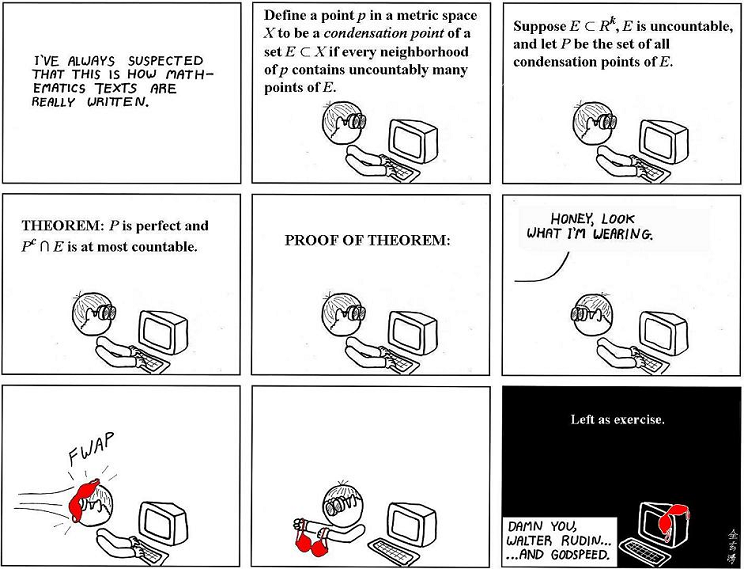
\includegraphics[width=14cm]{media/abstruse-goose-exercise.png}
\end{center}

I personally find most exercises to not be that interesting, and I've tried to keep boring ones to a minimum.
Regardless, I've tried hard to pick problems that are fun to think about and, when possible, to give them
the kind of flavor you might find on the IMO or Putnam (even when the underlying background is different).

\gim
Harder problems are marked with \chili's, like this paragraph.
For problems that have three chili's you should probably read the hint.

\section{Paper}
At the risk of being blunt,
\begin{moral}
Read this book with pencil and paper.
\end{moral}
Here's why:

\begin{center}
	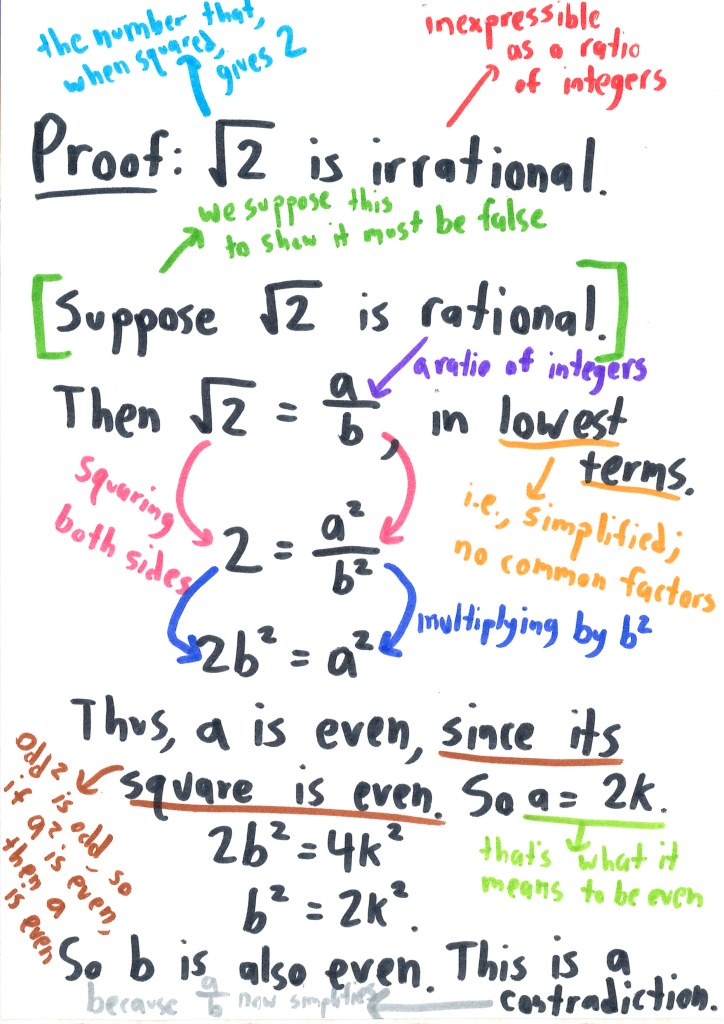
\includegraphics[width=0.5\textwidth]{media/read-with-pencil.jpg} \\
	{\footnotesize Source: \url{http://mathwithbaddrawings.com/2015/03/17/the-math-major-who-never-reads-math/}}
\end{center}
\textbf{You are not God.}
You cannot keep everything in your head.\footnote{
	See also \url{https://usamo.wordpress.com/2015/03/14/writing/} and the source above.
}
If you've printed out a hard copy, then write in the margins.
If you're trying to save paper, grab a notebook or something along with the ride.
Somehow, someway, make sure you can write. Thanks.


\section{Examples}
I am pathologically obsessed with examples.
In this book, I place all examples in large boxes to draw emphasis to them, which leads to some pages of the book simply consisting of sequences of boxes one after another. I hope the reader doesn't mind.

I also often highlight a ``prototypical example'' for some sections,
and reserve the color red for such a note.
The philosophy is that any time the reader sees a definition or a theorem about such an object, they should test it against the prototypical example.
If the example is a good prototype, it should be immediately clear why this definition is intuitive, or why the theorem should be true, or why the theorem is interesting, et cetera.

Let me tell you a secret.  When I wrote a definition or a theorem in this book, I would have to recall the exact statement from my memory, and my memory is very poor. So instead, I have to consider the prototypical example, and then only after that do I remember what the definition or the theorem is.
Incidentally, this is also how I learned all the definitions in the first place.
I hope you'll find it useful as well.

\section{SNSD}
Where appropriate, I have added math jokes from the
Tumblr \emph{Topological Girl's Generation}.
I hope you find them enjoyable.

\section{Topic Choices}
The appendix contains a list of resources I like and thoughts about
particular chapters and subjects and the like.
I encourage you to check it out.

The most important part of that is the first section.
For example, I learned category theory from \cite{ref:msci} and loved it,
and I don't think I could do a better job than it,
which is why I only barely touch on category theory here!

\section{Conventions and Notations}
This part describes some of the less familiar notations and definitions
and settles for once and for all some annoying issues (``is zero a natural number?'').

\subsection*{Sets and Equivalence Relations}
%\begin{definition}
%We denote by $\ZZ$, $\QQ$, $\RR$, and $\CC$ the set of integers,
%rational numbers, real numbers, and complex numbers, respectively.
%\end{definition}
$\NN$ is the set of \emph{positive} integers, not including $0$.

%\begin{definition}
%For sets $S$ and $T$, $S \setminus T$ is set subtraction.
%Also, $S \times T$ is the Cartesian product.
%\end{definition}

An \vocab{equivalence relation} on a set $X$ is a relation $\sim$
which is symmetric, reflexive, and transitive.
A equivalence relation partitions $X$ into several \vocab{equivalence classes}.
We will denote this by $X / {\sim}$.
An element of such an equivalence class is a \vocab{representative} of that equivalence class.


\subsection*{Functions}
Let $X \taking f Y$ be a function.

\begin{itemize}
\ii By $f\pre(T)$ I mean the \vocab{pre-image}
\[ f\pre(T) \defeq \left\{ x \in X \mid f(x) \in T \right\} \]
in contrast to the usual $f\inv(T)$; I only use $f\inv$ for an inverse \emph{function}.

By abuse of notation, we may abbreviate $f\pre(\{y\})$ to $f\pre(y)$.
We call $f\pre(y)$ a \vocab{fiber}.

\ii By $f``(S)$ I mean the \vocab{image}
\[ f``(S) \defeq \left\{ f(x) \mid x \in S \right\}. \]
The notation {``} is from set theory, and is meant to indicate ``point-wise''.
Most authors use $f(S)$, but this is abuse of notation,
and I prefer $f``(S)$ for emphasis.

\ii Sometimes functions $f : X \to Y$ are \emph{injective} or \emph{surjective};
I may emphasize this sometimes by writing $f : X \injto Y$ or $f : X \surjto Y$, respectively.
\end{itemize}

\subsection*{Rings}
All rings are commutative with a multiplicative identity $1$ unless otherwise specified.
We allow $0=1$ in general rings but not in integral domains.

\subsection*{Choice}
We accept the Axiom of Choice.


\Opensolutionfile{tex/backmatter/all-hints}
\Opensolutionfile{tex/backmatter/all-solns}

\part{Basic Algebra and Topology}
\chapter{What is a Group?}
A group is one of the most basic structures in higher mathematics.
In this chapter I will tell you only a bare minimum:
what a group is, and when two groups are the same.

\section{Definition and Examples of Groups}
\prototype{The additive group of integers $\ZZ_+$ and the cyclic group $\ZZ_m$. Just don't let yourself forget that most groups are non-commutative.}

A group consists of two pieces of data: a set $G$, and an associative binary operation $\star$ with some properties.
Before I write down the definition of a group, let me give two examples.

\begin{example}[Additive Integers]
	The pair $(\ZZ, +)$ is a group:
	$\ZZ = \left\{ \dots,-2,-1,0,1,2,\dots \right\}$ is the set
	and the associative operation is \emph{addition}.
	This operation has the following nice properties:
	\begin{itemize}
		\ii The element $0 \in \ZZ$ is an \emph{identity}:
		$a+0=0+a = a$ for any $a$.
		\ii Every element $a \in \ZZ$ has an additive \emph{inverse}: $a + (-a) = (-a) + a = 0$.
	\end{itemize}
	We call this group $\ZZ_+$.
\end{example}
\begin{example}[Nonzero Rationals]
	Let $\QQ^\times$ be the set of \emph{nonzero rational numbers}.
	The pair $(\QQ^\times, \cdot)$ is a group:
	the set is $\QQ^\times$
	and the associative operation is \emph{multiplication}.

	Again we see the same two nice properties.
	\begin{itemize}
		\ii The element $1 \in \QQ^\times$ is an \emph{identity}:
		for any rational number, $a \cdot 1 = 1 \cdot a = a$.
		\ii For any rational number $x \in \QQ^\times$,
		we have an inverse $\frac{1}{x}$, such that
		\[ x \cdot \frac 1x = \frac 1x \cdot x = 1. \]
	\end{itemize}
\end{example}

From this I bet you can already guess what the definition of a group is.
\begin{definition}
	A \vocab{group} is a pair $G = (G, \star)$
	consisting of a set of elements $G$, and an associative
	binary operation $\star$ on $G$, with the following properties.
	\begin{itemize}
		\ii $G$ has an \vocab{identity element}, usually denoted $1_G$
		or just $1$, with the property that
		\[ 1_G \star g = g \star 1_G = g \text{ for all $g \in G$}. \]
		\ii Each element $g \in G$ has an \vocab{inverse}, that is, an element $h \in G$ such that \[ g \star h = h \star g = 1_G. \]
	\end{itemize}
	\label{def:group}
\end{definition}

\begin{figure}[ht]
	\centering
	\includegraphics[height=8cm]{/home/evan/Pictures/TopologicalGG/are-you-my-identity.jpg}
	\caption{The identity of a group is generally written ``$1$''.}
\end{figure}

Now that I've made clear what the criteria of a group are, let us write down some non-examples of groups.

\begin{example}[Non-Examples of Groups]
	\listhack
	\begin{itemize}
		\ii The pair $(\QQ, \times)$ is NOT a group.
		While there is an identity element, the element $0 \in \QQ$
		does not have an inverse.
		\ii The pair $(\ZZ, \times)$ is also NOT a group. (Why?)
		\ii Let $\Mat_{2 \times 2}$ be the set of $2 \times 2$ matrices.
		Then $(\Mat_{2 \times 2}, \times)$ (where $\times$ is matrix multiplication) is NOT a group. Indeed, even though we have an identity matrix
		\[ \left(
			\begin{array}{cc}
				1 & 0 \\ 0 & 1
			\end{array}
			\right)
		\]
		we still run into the same issue as before:
		the zero matrix does not have a multiplicative inverse.
		\ii Even if we delete the zero matrix from the set,
		the resulting structure is still not a group:
		those of you that know even a little linear algebra
		might recall that any matrix with determinant zero
		cannot have an inverse.
	\end{itemize}
\end{example}

Let's resume writing down examples of groups.

\begin{example}
	[General Linear Group]
	Let $n$ be a positive integer.
	Then $\GL_n(\RR)$ is defined as the set of $n \times n$ real matrices which have nonzero determinant.
	It turns out that with this condition, every matrix does indeed have an inverse, so $(\GL_n(\RR), \times)$ is a group, called the
	\vocab{general linear group}.
	(The fact that $\GL_n(\RR)$ is closed under $\times$ follows from the linear algebra fact that $\det (AB) = \det A \det B$.)
\end{example}
\begin{example}
	[Special Linear Group]
	Following the example above, let $\SL_n(\RR)$ denote 
	the set of $n \times n$ matrices whose determinant is actually $1$.
	Again, for linear algebra reasons
	it turns out that $(\SL_n(\RR), \times)$ is also a group, called the \vocab{special linear group}.
\end{example}

\begin{example}
	[Complex Unit Circle]
	Let $S^1$ denote the set of complex numbers $z$ with absolute value one; that is
	\[ S^1 \defeq \left\{ z \in \CC \mid \left\lvert z \right\rvert = 1 \right\}. \]
	Then $(S^1, \times)$ is a group because
	\begin{itemize}
		\ii The complex number $1 \in S^1$ serves as the identity, and
		\ii Each complex number $z \in S^1$ has an inverse $\frac 1z$ which is also in $S^1$, since $\left\lvert z\inv \right\rvert = \left\lvert z \right\rvert\inv = 1$.
	\end{itemize}
	There is one thing I ought to also check: that $z_1 \times z_2$ is actually still in $S^1$.
	But this follows from the fact that $\left\lvert z_1z_2 \right\rvert = \left\lvert z_1 \right\rvert \left\lvert z_2 \right\rvert = 1$.
\end{example}

\begin{example}
	[Adding mod $n$]
	Here is an example from number theory:
	Let $n > 1$ be an integer,
	and consider the residues modulo $n$.
	These form a group under addition.
	We call this the \vocab{cyclic group of order $n$},
	and abbreviate it as $\Zc n$, with element $\ol 0, \ol 1, \dots$.
	\label{def:cyclic_group}
\end{example}
\begin{example}
	[Multiplication mod $p$]
	Let $p$ be a prime.
	Consider the \emph{nonzero residues modulo $p$},
	which we denote by $\Zm p$
	Then $\left( \Zm p, \times \right)$ is a group.
	\label{def:mult_mod_p}
\end{example}
\begin{ques}
	Why do we need the fact that $p$ is prime?
\end{ques}

The next two examples are fairly important ones:

\begin{example}
	[Symmetric Groups]
	Let $S_n$ be the set of permutations of $\left\{ 1,\dots,n \right\}$.
	By viewing these permutations as functions from $\left\{ 1,\dots,n \right\}$ to itself, we can consider \emph{compositions} of permutations.
	Then the pair $(S_n, \circ)$ (here $\circ$ is function composition)
	is also a group, because
	\begin{itemize}
		\ii There is an identity permutation, and
		\ii Each permutation has an inverse.
	\end{itemize}
	The group $S_n$ is called the \vocab{symmetric group} on $n$ elements.
\end{example}

\begin{example}
	[Dihedral Group]
	The \vocab{dihedral group of order $2n$} is the group of symmetries of
	a regular $n$-gon $A_1A_2 \dots A_n$, which includes rotations and reflections.
	It consists of the following $2n$ elements:
	\[ \left\{ 1, r, r^2, \dots, r^{n-1}, s, sr, sr^2, \dots, sr^{n-1} \right\}. \]
	The element $r$ corresponds to rotating the $n$-gon by $\frac{2\pi}{n}$,
	while $s$ corresponds to reflecting it across the line $OA_1$
	(here $O$ is the center of the polygon).
	So $rs$ mean ``reflect then rotate'' (like with function composition,
	we read from right to left).

	In particular, $r^n = s^2 = 1$. You can also see that $r^ks = sr^{-k}$.
\end{example}

Trivia: the dihedral group $D_{12}$ is my favorite example of a non-abelian group,
and is the first group I try for any exam question of the form ``find an example\dots''.
Here is a picture of some elements of $D_{10}$.
\begin{center}
	\begin{asy}
		size(12cm);
		picture aoeu(string a, string b, string c, string d, string e,
					string x) {
			draw(dir(0)--dir(72)--dir(144)--dir(216)--dir(288)--cycle);
			MP(a, dir(0), dir(0));
			MP(b, dir(72), dir(72));
			MP(c, dir(144), dir(144));
			MP(d, dir(216), dir(216));
			MP(e, dir(288), dir(288));
			MP(x, origin, origin);
			return CC();
		}
		picture one = aoeu("1", "2", "3", "4", "5", "1");
		picture r = aoeu("5", "1", "2", "3", "4", "r");
		picture s = aoeu("1", "5", "4", "3", "2", "s");
		picture sr = aoeu("5", "4", "3", "2", "1", "sr");
		picture rs = aoeu("2", "1", "5", "4", "3", "rs");
		add(shift( (0,0) ) * one);
		add(shift( (3,0) ) * r);
		add(shift( (6,0) ) * s);
		add(shift( (9,0) ) * sr);
		add(shift( (12,0) ) * rs);
	\end{asy}
\end{center}


Note that the last two groups all share a non-property: the group operation is not in general commutative!
We leave these as a warning for the reader.
\begin{definition}
We say that a group is \vocab{abelian} if the operation is commutative and \vocab{non-abelian} otherwise.
\end{definition}

\begin{example}
	[Products of Groups]
	Let $(G, \star)$ and $(H, \ast)$ be groups.
	We can define a \vocab{product group} $(G \times H, {\cdot})$, as follows.
	The elements of the group will be ordered pairs $(g,h) \in G \times H$.
	Then
	\[ (g_1, h_1) \cdot (g_2, h_2) = (g_1 \star g_2, h_1 \ast h_2) \in G \times H
		\]
	is the group operation.
	\label{def:product_group}
\end{example}
\begin{ques}
	What are the identity and inverses of the product group?
\end{ques}

\begin{example}
	[Trivial Group]
	The \vocab{trivial group}, often denoted $0$ or $1$,
	is the group with only an identity element.
	I will use the notation $\{1\}$.
\end{example}

\begin{ques}
	Which of these are groups?
	\begin{enumerate}[(a)]
		\ii Rational numbers with odd denominators, where the operation is addition.
		\ii The set of rational numbers with denominator at most $2$, where the operation is addition.
		\ii The set of rational numbers with denominator at most $2$, where the operation is multiplication.
		\ii The set of nonnegative integers, where the operation is addition.
	\end{enumerate}
\end{ques}


\section{Properties of Groups}
\prototype{$\Zm p$ is possibly best.}
\begin{abuse}
	From now on, we'll often refer to a group $(G, \star)$ by just $G$.
	Moreover, we'll abbreviate $a \star b$ to just $ab$.
	Also, because the operation $\star$ is associative,
	we will omit unnecessary parentheses: $(ab)c = a(bc) = abc$.
\end{abuse}
\begin{abuse}
	From now on, for any $g \in G$ and $n \in \NN$ we abbreviate
	\[ g^n
		=
		\underbrace{g \star \dots \star g}_{\text{$n$ times}}.\]
	Moreover, we let $g\inv$ denote the inverse of $g$,
	and $g^{-n} = (g\inv)^n$.
\end{abuse}

If you did functional equations at the IMO, you might know that you can actually determine a lot about a function just by knowing a few properties of it.
For example, if you know that $f : \QQ \to \RR$ satisfies $f(x+y) = f(x) + f(y)$, then you actually can show that $f(x) = cx$ for some $c \in \RR$.
(This is called Cauchy's functional equation.)

In the same vein, we can try to deduce some properties that a group must have just from \Cref{def:group}.
(In fact, this really is a functional equation: $\star$ is just a function $G \times G \to G$.)

It is a law in Guam and 37 other states that I now state the following proposition.
\begin{fact}
	Let $G$ be a group.
	\begin{enumerate}[(a)]
		\ii The identity of a group is unique.
		\ii The inverse of any element is unique.
		\ii For any $g \in G$, $(g\inv)\inv = g$.
	\end{enumerate}
\end{fact}
\begin{proof}
	Omitted because it's easy, boring, and everywhere.
\end{proof}

Now we state a slightly more useful proposition.
\begin{proposition}
	Let $G$ be a group, and $a,b \in G$.
	Then $(ab)\inv = b\inv a\inv$.
\end{proposition}
\begin{proof}
	Direct computation. We have
	\[ (ab)(b\inv a\inv)
		= a (bb\inv) a\inv = aa\inv = 1_G. \]
	Hence $(ab)\inv = b\inv a\inv$.
\end{proof}

Finally, we state a very important lemma about groups,
which highlights why having an inverse is so valuable.
\begin{lemma}
	Let $G$ be a group, and pick a $g \in G$. 
	Then the map $G \to G$ given by
	$x \mapsto gx$
	is a bijection.
	\label{lem:group_mult_biject}
\end{lemma}
\begin{exercise}
	Check this. (Show injectivity and surjectivity directly.)
\end{exercise}
\begin{example}
	Let $G = \Zm 7$ (as in \Cref{def:mult_mod_p}) and pick $g=3$.
	The above lemma states that the map $x \mapsto 3 \cdot x$ is a bijection, and we can see this explicitly:
	\begin{align*}
		1 &\overset{\times 3}{\longmapsto} 3 \pmod 7 \\
		2 &\overset{\times 3}{\longmapsto} 6 \pmod 7 \\
		3 &\overset{\times 3}{\longmapsto} 2 \pmod 7 \\
		4 &\overset{\times 3}{\longmapsto} 5 \pmod 7 \\
		5 &\overset{\times 3}{\longmapsto} 1 \pmod 7 \\
		6 &\overset{\times 3}{\longmapsto} 4 \pmod 7.
	\end{align*}
\end{example}


The fact that the map is injective is often called the \vocab{cancellation law}.
(Why do you think so?)

\section{Isomorphisms}
\prototype{$\ZZ_+ \cong 10\ZZ_+$.}
First, let me talk about what it means for groups to be isomorphic.
Consider the following two groups:
\begin{itemize}
	\ii $\ZZ_+ = (\left\{ \dots,-2,-1,0,1,2,\dots \right\}, +)$.
	\ii $10\ZZ_+ = (\left\{ \dots, -20, -10, 0, 10, 20, \dots \right\}, +)$.
\end{itemize}
These groups are ``different'', but only superficially so -- you might even say they only differ in the names of the elements.
Think about what this might mean formally for a moment.

Specifically the map
\[ \phi : \ZZ_+ \to 10 \ZZ_+  \text{ by } x \mapsto 10 x \]
is a bijection of the underlying sets which respects the group action.
In symbols,
\[ \phi(x + y) = \phi(x) + \phi(y). \]
In other words, $\phi$ is a way of re-assigning names of the elements
without changing the structure of the group.
That's all just formalism for capturing the obvious fact that $\ZZ_+$ and $10 \ZZ_+$ are the same thing.

Now, let's do the general definition.
\begin{definition}
	Let $G = (G, \star)$ and $H = (H, \ast)$ be groups.
	A bijection $\phi : G \to H$ is called an \vocab{isomorphism} if
	\[ \phi(g_1 \star g_2) = \phi(g_1) \ast \phi(g_2) \quad
		\text{for all $g_1, g_2 \in G$}. \]
	If there exists an isomorphism from $G$ to $H$,
	then we say $G$ and $H$ are \vocab{isomorphic} and write $G \cong H$.
\end{definition}
Note that in this definition, the left-hand side $\phi(g_1 \star g_2)$ uses the operation of $G$ while the right-hand side uses the operation of $H$.

\begin{example}
	[Examples of Isomorphims]
	Let $G$ and $H$ be groups.  We have the following isomorphisms.
	\begin{enumerate}[(a)]
		\ii $\ZZ_+ \cong 10 \ZZ_+$, as above.
		\ii There is an isomorphism
		\[ G \times H \cong H \times G\]
		by the map $(g,h) \mapsto (h,g)$.
		\ii The identity map $\id : G \to G$
		is an isomorphism, hence $G \cong G$.
		\ii There is another isomorphism of $\ZZ_+$ to itself: send every $x$ to $-x$.
	\end{enumerate}
\end{example}
\begin{example}
	[Primitive Roots Modulo $7$]
	As a nontrivial example, we claim that $\Zc 6 \cong \Zm 7$.
	The bijection is
	\[ \phi(\text{$a$ mod $6$}) = \text{$3^a$ mod $7$}. \]
	To check that this is an isomorphism, we need to verify several things.
	\begin{itemize}
		\ii First, we need to check this map actually makes sense:
		why is it the case that if $a \equiv b \pmod 6$, then $3^a \equiv 3^b \pmod 7$?
		The reason is that Fermat's Little Theorem guarantees that $3^6 \equiv 1 \pmod 7$.
		\ii Next, we need to check that this map is a bijection.
		You can do this explicitly:
		\[ (3^1, 3^2, 3^3, 3^4, 3^5, 3^6)
			\equiv (3,2,6,4,5,1) \pmod 7. \]
		\ii Finally, we need to verify that this map respects the group action.
		In other words, we want to see that
		$\phi(a+b) = \phi(a) \phi(b)$
		since the operation of $\Zc 6$ is addition
		while the operation of $\Zm 7$ is multiplication.
		That's just saying that $3^{a+b} \equiv 3^a 3^b \pmod 7$,
		which is true.
	\end{itemize}
\end{example}
\begin{example}
	[Primitive Roots] More generally, for any prime $p$,
	there exists an element $g \in \Zm p$ called a \vocab{primitive root} modulo $p$ such that $1, g, g^2, \dots, g^{p-2}$ are all different modulo $p$.
	One can show by copying the above proof that
	\[ \Zc {p-1} \cong \Zm p \text{ for all primes $p$}. \]
	The example above was the special case $p=7$ and $g=3$.
\end{example}
\begin{exercise}
	Assuming the existence of primitive roots,
	establish the isomorphism $\Zc {p-1} \cong \Zm p$ as above.
\end{exercise}

It's not hard to see that $\cong$ is an equivalence relation (why?).
Moreover, because we really only care about the structure of groups,
we'll usually consider two groups to be the same when they are isomorphic.
So phrases such as ``find all groups'' really means ``find all groups up to isomorphism''.

\section{Orders of Groups, and Lagrange's Theorem}
\prototype{$\Zm p$.}

As is typical in math, we use the word ``order'' for way too many things.
In groups, there are two notions of order.
\begin{definition}
	The \vocab{order of a group} $G$ is the number of elements of $G$.
	We denote this by $\left\lvert G \right\rvert$.
	Note that the order may not be finite, as in $\ZZ_+$.
	We say $G$ is a \vocab{finite group} just to mean that $\left\lvert G \right\rvert$ is finite.
\end{definition}
\begin{example}[Order of the Cyclic Group]
	For a prime $p$, $\left\lvert \Zm p \right\rvert = p-1$.
	In other words, the order of $\Zm p$ is $p-1$.
	As another example, the order of the symmetric group $S_n$ is $\left\lvert S_n \right\rvert = n!$
	and the order dihedral group $D_{2n}$ is $2n$.
\end{example}

\begin{definition}
	The \vocab{order of an element} $g \in G$ is the smallest positive integer $n$
	such that $g^n = 1_G$, or $\infty$ if no such $n$ exists.
	We denote this by $\ord g$.
\end{definition}
\begin{example}[Examples of Orders]
	The order of $-1$ in $\QQ^\times$ is $2$,
	while the order of $1$ in $\ZZ_+$ is infinite.
\end{example}
\begin{ques}
	Find the order of each of the six elements of $\Zc 6$,
	the cyclic group on six elements.
	(See \Cref{def:cyclic_group} if you've forgotten what $\Zc 6$ means.)
\end{ques}
\begin{example}[Primitive Roots]
	If you know olympiad number theory, this coincides with the definition of an order of a residue mod $p$.
	That's why we use the term ``order'' there as well.
	In particular, a primitive root is precisely an element $g \in \Zm p$
	such that $\ord g = p-1$.
\end{example}
You might also know that if $x^n \equiv 1 \pmod p$,
then the order of $x \pmod p$ must divide $n$.
The same is true in a general group for exactly the same reason.
\begin{fact}
	If $g^n = 1_G$ then $\ord g$ divides $n$.
\end{fact}
Also, you can show that any element of a finite group has an order.
The proof is just an olympiad-style pigeonhole argument: consider the infinite sequence $1_G, g, g^2, \dots$, and find two elements that are the same.
\begin{fact}
	Let $G$ be a finite group.
	For any $g \in G$, $\ord g$ is finite.
\end{fact}

What's the last property of $\Zm p$ that you know from olympiad math?
We have Fermat's Little Theorem: for any $a$, we have $a^{p-1} \equiv 1 \pmod p$.
This is no coincidence: exactly the same thing is true in a more general setting.

\begin{theorem}
	[Lagrange's Theorem]
	Let $G$ be any finite group.
	Then $x^{\left\lvert G \right\rvert} = 1_G$ for any $x \in G$.
\end{theorem}
Keep this result in mind!

\section{Subgroups}
\prototype{$\SL_n(\RR)$ is a subgroup of $\GL_n(\RR)$.}
Earlier we saw that $\GL_n(\RR)$, the $n \times n$ matrices with nonzero determinant, formed a group under matrix multiplication.
But we also saw that a subset of $\GL_n(\RR)$, namely $\SL_n(\RR)$, also formed a group with the same operation.
For that reason we say that $\SL_n(\RR)$ is a subgroup of $\GL_n(\RR)$.
And this definition generalizes in exactly the way you expect.

\begin{definition}
	Let $G = (G, \star)$ be a group.
	A \vocab{subgroup} of $G$ is exactly what you would expect it to be:
	a group $H = (H, \star)$ where $H$ is a subset of $G$.
	It's a \vocab{proper subgroup} if $H \neq G$.
\end{definition}


\begin{remark*}
	To specify a group $G$, I needed to tell you both what the set $G$ was and the operation $\star$ was.
	But to specify a subgroup $H$ of a given group $G$, I only need to tell you who its elements are: the operation of $H$ is just inherited from the operation of $G$.
\end{remark*}

\begin{example}
	[Examples of Subgroups]
	\listhack
	\begin{enumerate}[(a) ]
		\ii $2\ZZ_+$ is a subgroup of $\ZZ_+$, which is isomorphic to $\ZZ_+$ itself!
		\ii Consider again $S_n$, the symmetric group on $n$ elements.
		Let $T$ be the set of permutations $\tau$ for which $\tau(n) = n$.
		Then $T$ is a subgroup of $S_n$;
		in fact, it is isomorphic to $S_{n-1}$.
		\ii Consider the group $G \times H$ (\Cref{def:product_group})
		and the elements $ \left\{ (g, 1_H) \mid g \in G \right\} $.
		This is a subgroup of $G \times H$ (why?).
		In fact, it is isomorphic to $G$
		by the isomorphism $(g,1_H) \mapsto g$.
	\end{enumerate}
\end{example}
\begin{example}
	[Stupid Examples of Subgroups]
	For any group $G$, the trivial group $\{1_G\}$
	and the entire group $G$ are subgroups of $G$.
\end{example}
%\begin{example}
%	[Center of a Group]
%	Let $G$ be a group.
%	Its \vocab{center}, denoted $Z(G)$, is the set $x \in G$ such that
%	$gx = xg$ for every $g \in G$; in other words, it is the set of
%	$x \in G$ which commute with every element of $G$.
%\end{example}
%You can check the center is indeed a group (some boring details\dots).

Next is an especially important example that we'll talk about more in later chapters.
\begin{example}[Subgroup Generated by an Element]
	Let $x$ be an element of a group $G$.
	Consider the set
	\[ \left<x\right> = \left\{ \dots, x^{-2}, x^{-1}, 1, x, x^2, \dots \right\}. \]
	This is also a subgroup of $G$, called the subgroup generated by $x$.
\end{example}
\begin{exercise}
	If $\ord x = 2015$, what is the above subgroup equal to?
	What if $\ord x = \infty$?
\end{exercise}

Finally, we present some non-examples of subgroups.
\begin{example}[Non-Examples of Subgroups]
	Consider the group $\ZZ_+$.
	\begin{enumerate}[(a)]
		\ii The set $\left\{ 0,1,2,\dots \right\}$ is not a subgroup of $\ZZ_+$ because it does not contain inverses.
		\ii The set $\{ n^3 \mid n \in \ZZ \} = \{ \dots, -8, -1, 0, 1, 8, \dots \}$ is not a subgroup
		because it is not closed under addition; the sum of two cubes is not in general a cube.
		\ii The empty set $\varnothing$ is not a subgroup of $\ZZ_+$ because it lacks an identity element.
	\end{enumerate}
\end{example}

\section{Groups of Small Orders}
Just for fun, here is a list of all groups of order less than or equal to ten
(up to isomorphism, of course).
\begin{enumerate}
	\ii The only group of order $1$ is the trivial group.
	\ii The only group of order $2$ is $\Zc 2$.
	\ii The only group of order $3$ is $\Zc 3$.
	\ii The only groups of order $4$ are
	\begin{itemize}
		\ii $\Zc 4$, the cyclic group on four elements,
		\ii $\Zc 2 \times \Zc 2$, called the Klein Four Group.
	\end{itemize}
	\ii The only group of order $5$ is $\Zc 5$.
	\ii The groups of order six are
	\begin{itemize}
		\ii $\Zc 6$, the cyclic group on six elements.
		\ii $S_3$, the permutation group of three elements.
		This is the first non-abelian group.
	\end{itemize}
	Some of you might wonder where $\Zc 2 \times \Zc 3$ is.
	All I have to say is: Chinese Remainder Theorem!

	Those of you who also know what the dihedral group $D_6$ is might also
	be wondering where that is. It's actually isomorphic to $S_3$.
	\ii The only group of order $7$ is $\Zc 7$.
	\ii The groups of order eight are more numerous.
	\begin{itemize}
		\ii $\Zc 8$, the cyclic group on eight elements.
		\ii $\Zc 4 \times \Zc 2$.
		\ii $\Zc 2 \times \Zc 2 \times \Zc 2$.
		\ii $D_8$, the dihedral group with eight elements, which is not abelian.
		\ii The non-abelian group $Q_8$ of \emph{quaternions}.
	\end{itemize}
	\ii The groups of order nine are
	\begin{itemize}
		\ii $\Zc 09$, the cyclic group on nine elements.
		\ii $\Zc 3 \times \Zc 3$.
	\end{itemize}
	\ii The groups of order $10$ are
	\begin{itemize}
		\ii $\ZZ_{10} \cong \ZZ_5 \times \ZZ_2$ (again Chinese Remainder Theorem).
		\ii $D_{10}$, the dihedral group with $10$ elements.
		This group is non-abelian.
	\end{itemize}
\end{enumerate}

\section\problemhead
\begin{problem}
	What is the joke in the following figure?
	\begin{center}
		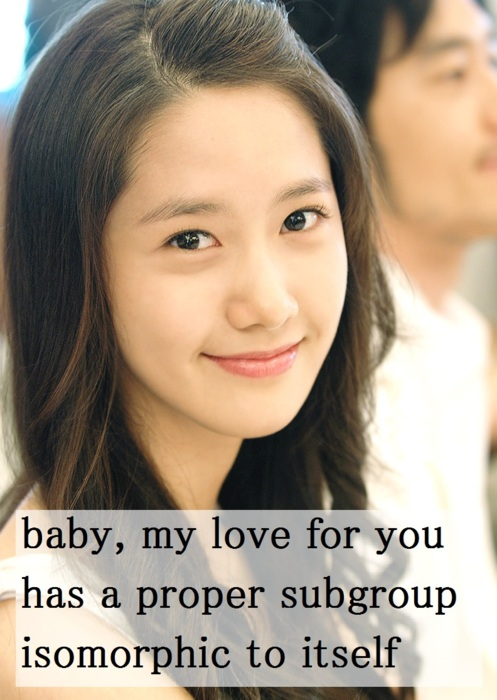
\includegraphics[height=8cm]{/home/evan/Pictures/TopologicalGG/love-proper-isomorphic-subgroup.jpg}
		%\caption{$\heartsuit$ is a group, $G \subsetneq \heartsuit$ a subgroup and $G \cong \heartsuit$.}
	\end{center}
	\begin{hint}
		Orders.
	\end{hint}
	\begin{sol}
		The point is that $\heartsuit$ is a group, $G \subsetneq \heartsuit$ a subgroup and $G \cong \heartsuit$.
		This can only occur if $\left\lvert \heartsuit \right\rvert = \infty$;
		otherwise, a proper subgroup would have strictly smaller size than the original.
	\end{sol}
\end{problem}

\begin{problem}
	Prove Lagrange's Theorem in the special case
	that $G$ is a finite abelian group.
	\begin{hint}
		Copy the proof of Fermat's Little Theorem, using
		\Cref{lem:group_mult_biject}.)
	\end{hint}
	\begin{sol}
		Let $\{g_1, g_2, \dots, g_n\}$ denote the elements of $G$.
		For any $g \in G$, this is the same as the set $\{gg_1, \dots, gg_n\}$.
		Taking the entire product and exploiting commutativity gives
		$g^n \cdot g_1g_2 \dots g_n = g_1g_2 \dots g_n$, hence $g^n=1$.
	\end{sol}
\end{problem}

\begin{problem}
	Show that $D_6 \cong S_3$.
	\begin{hint}
		Decide where the isomorphism should send $r$ and $s$,
		and the rest will follow through.
	\end{hint}
	\begin{sol}
		One can check manually that $D_6 \cong S_3$,
		using the map $r \mapsto (1 \; 2 \; 3)$ and $s \mapsto (1 \; 2)$.
	\end{sol}
\end{problem}

\begin{sproblem}
	Let $p$ be a prime.
	Show that the only group of order $p$ is $\ZZ_p$.
	\begin{hint}
		Generated groups.
	\end{hint}
	\begin{sol}
		Let $G$ be a group of order $p$, and $1 \neq g \in G$.
		Look at the group $H$ generated by $g$ and use Lagrange's Theorem.
	\end{sol}
\end{sproblem}

\begin{dproblem}
	[Cayley's Theorem]
	\gim
	Let $G$ be a finite group.\footnote{
		In other words, permutation groups can be arbitrarily weird.
		I remember being highly unsettled by this theorem when I first heard of it.}
	Show that there exists a positive integer $n$ such that
	\begin{enumerate}[(a)]
		\ii (Cayley's Theorem) $G$ is isomorphic to some subgroup of the symmetric group $S_n$.
		\ii (Representation Theory) $G$ is isomorphic to some subgroup of
		of the general linear group $\GL_n(\RR)$.
		(This is the group of invertible $n \times n$ matrices.)
	\end{enumerate}
	\label{thm:cayley_theorem}
	\begin{hint}
		Use $n = \left\lvert G \right\rvert$.
	\end{hint}
	\begin{sol}
		The idea is that each element $g \in G$ can be thought of as a permutation
		$G \to G$ by $x \mapsto gx$.
	\end{sol}
\end{dproblem}

\begin{problem}
	[MOP 2006] \gim
	There are $n$ markers, each with one side white and the other side black.
	In the beginning, these $n$ markers are aligned in a row so that their white sides are all up.
	In each step, if possible, we choose a marker whose white side is up (but not one of the outermost markers),
	remove it, and reverse the closest marker to the left of it and also reverse the closest marker to the right of it.
	
	Prove that if $n \equiv 1 \pmod 3$ it's impossible to reach a state with only two markers remaining.
	% http://www.artofproblemsolving.com/Forum/viewtopic.php?f=41&t=90046&p=3573800
	\begin{hint}
		Draw inspiration from $D_6$.
	\end{hint}
	\begin{sol}
		We have $www = bb$, $bww = wb$, $wwb = bw$, $bwb = ww$.
		Interpret these as elements of $D_6$.
	\end{sol}
\end{problem}


%\begin{problem}[Hard]
%	Exhibit two groups $G$ and $H$ which are not isomorphic with the property that
%	for every positive integer $n$,
%	the number of elements $g \in G$ with $\ord g = n$
%	equals the number of elements $h \in H$ with $\ord h = n$.
%\end{problem}

\chapter{What is a space?}
At the time of writing, I'm convinced that metric topology is
the morally correct way to motivate point-set topology
as well as to generalize normal calculus.
Also, ``metric'' is a fun word to say.
So here is my best attempt.

The concept of a metric space is very ``concrete'', and lends itself easily to visualization. Hence throughout this chapter you should draw lots of pictures as you learn about new objects, like convergent sequences, open sets, closed sets, and so on.

\section{Definition and examples of metric spaces}
\prototype{$\RR^2$, with the Euclidean metric.}
\begin{definition}
	A \vocab{metric space} is a pair $(M, d)$ consisting of
	a set of points $M$
	and a \vocab{metric} $d : M \times M \to \mathbb R_{\ge 0}$.
	The distance function must obey:
	\begin{itemize}
		\ii For any $x,y \in M$, we have $d(x,y) = d(y,x)$; i.e.\ $d$ is symmetric.
		\ii The function $d$ must be \vocab{positive definite}
		which means that $d(x,y) \ge 0$ with equality if and only if $x=y$.
		\ii The function $d$ should satisfy the \vocab{triangle inequality}: for all $x,y,z \in M$,
		\[ d(x,z) + d(z,y) \ge d(x,y). \]
	\end{itemize}
\end{definition}
\begin{abuse}
	Just like with groups, we will abbreviate $(M,d)$ as just $M$.
\end{abuse}
\begin{example}[Metric spaces of $\RR$]
	\listhack
	\begin{enumerate}[(a)]
		\ii The real line $\RR$ is a metric space under the metric $d(x,y) = \left\lvert x-y \right\rvert$.
		\ii The interval $[0,1]$ is also a metric space with the same distance function.
		\ii In fact, any subset $S$ of $\RR$ can be made into a metric space in this way.
	\end{enumerate}
\end{example}
\begin{example}[Metric spaces of $\RR^2$]
	\listhack
	\begin{enumerate}[(a)]
		\ii We can make $\RR^2$ into a metric space by imposing the Euclidean distance function
		\[ d\left( (x_1, y_1), (x_2, y_2) \right) = \sqrt{(x_1-x_2)^2 + (y_1-y_2)^2}. \]
		\ii Just like with the first example, any subset of $\RR^2$ also becomes a metric space after we inherit it.
		The unit disk, unit circle, and the unit square $[0,1]^2$
		are special cases.
	\end{enumerate}
\end{example}
\begin{example}[Taxicab on $\RR^2$]
	It is also possible to place the \vocab{taxicab distance} on $\RR^2$:
	\[ d\left( (x_1, y_1), (x_2, y_2) \right) = 
		\left\lvert x_1-x_2 \right\rvert + \left\lvert y_1-y_2 \right\rvert.
		\]
	For now, we will use the more natural Euclidean metric.
\end{example}

\begin{example}[Metric spaces of $\RR^n$]
	We can generalize the above examples easily.
	Let $n$ be a positive integer.
	\begin{enumerate}[(a)]
		\ii We let $\RR^n$ be the metric space whose points are points in $n$-dimensional Euclidean space,
		and whose metric is the Euclidean metric
		\[
			d\left( 
			\left( a_1, \dots, a_n \right), \left( b_1, \dots, b_n \right)
			\right)
			= \sqrt{(a_1-b_1)^2 + \dots + (a_n-b_n)^2}.
		\]
		This is the $n$-dimensional \vocab{Euclidean space}.
		\ii The open \vocab{unit ball} $B^{n}$ is the subset of $\RR^n$
		consisting of those points $\left( x_1, \dots, x_n \right)$
		such that $x_1^2 + \dots + x_n^2 < 1$.
		\ii The \vocab{unit sphere} $S^{n-1}$ is the subset of $\RR^n$
		consisting of those points $\left( x_1, \dots, x_n \right)$
		such that $x_1^2 + \dots + x_n^2 = 1$, with the inherited metric.
		(The superscript $n-1$ indicates that $S^{n-1}$ is an $n-1$ dimensional space,
		even though it lives in $n$-dimensional space.)
		For example, $S^1 \subseteq \RR^2$ is the unit circle,
		whose distance between two points is the length of the chord joining them.
		You can also think of it as the ``boundary'' of the unit ball $B^n$.
	\end{enumerate}
\end{example}
\begin{example}
	[Function space] 
	We can let $M$ be the space of
	integrable functions $f : [0,1] \to \RR$ and define the metric
	by $d(f,g) = \int_0^1 \left\lvert f-g \right\rvert \; dx$.
\end{example}

Here is a slightly more pathological example.
\begin{example}
	[Discrete space]
	Let $S$ be any set of points (either finite or infinite).
	We can make $S$ into a \vocab{discrete space} by declaring
	\[
		d(x,y)
		=
		\begin{cases}
			1 & \text{if $x \neq y$} \\
			0 & \text{if $x = y$}.
		\end{cases}
	\]
	If $\left\lvert S \right\rvert = 4$ you might think of this space
	as the vertices of a regular tetrahedron, living in $\RR^3$.
	But for larger $S$ it's not so easy to visualize\dots
\end{example}
\begin{example}[Graphs are metric spaces]
	Any connected simple graph $G$ can be made into a metric space
	by defining the distance between two vertices to be the
	graph-theoretic distance between them.
	(The discrete metric is the special case when $G$ is the complete graph on $S$.)
\end{example}
\begin{ques}
	Check the conditions of a metric space for the metrics on the discrete space
	and for the connected graph.
\end{ques}

\begin{abuse}
	From now on, we will refer to $\RR^n$ with the Euclidean metric
	by just $\RR^n$.
	Moreover, if we wish to take the metric space for a subset $S \subseteq \RR^n$
	with the inherited metric, we will just write $S$.
\end{abuse}

\section{Convergence in metric spaces}
\prototype{The sequence $\frac1n$ (for $n=1,2,\dots$) in $\RR$.}

Since we can talk about the distance between two points, we can talk about what it means for a sequence of points to converge.
This is the same as the typical epsilon-delta definition, with absolute values replaced by the distance function.

\begin{definition}
	Let $(x_n)_{n \ge 1}$ be a sequence of points in a metric space $M$.
	We say that $x_n$ \vocab{converges} to $x$ if the following condition holds:
	for all $\eps > 0$, there is an integer $N$ (depending on $\eps$)
	such that $d(x_n, x) < \eps$ for each $n \ge N$.
	This is written \[ x_n \to x \] or more verbosely as \[ \lim_{n \to \infty} x_n = x. \]
	We say that a sequence converges in $M$ if it converges to a point in $M$.
\end{definition}
You should check that this definition coincides with your intuitive notion of ``converges''.
\begin{abuse}
	If the parent space $M$ is understood, we will allow ourselves
	to abbreviate ``converges in $M$'' to just ``converges''.
	However, keep in mind that convergence is defined relative to the parent space;
	the ``limit'' of the space must actually be a point in $M$ for a sequence to converge.
\end{abuse}

\begin{center}
	\begin{asy}
		size(9cm);
		Drawing("x_1", (-9,0.1), dir(90));
		Drawing("x_2", (-6,0.8), dir(90));
		Drawing("x_3", (-5,-0.3), dir(90));
		Drawing("x_4", (-2, 0.8), dir(90));
		Drawing("x_5", (-1.7, -0.7), dir(-90));
		Drawing("x_6", (-0.6, -0.3), dir(225));
		Drawing("x_7", (-0.4, 0.3), dir(90));
		Drawing("x_8", (-0.25, -0.24), dir(-90));
		Drawing("x_9", (-0.12, 0.1), dir(45));
		dot("$x$", (0,0), dir(-45), blue);
		draw(CR(origin, 1.5), blue+dashed);
	\end{asy}
\end{center}

\begin{example}
	Consider the sequence
	$x_1 = 1$, $x_2 = 1.4$, $x_3 = 1.41$, $x_4 = 1.414$, \dots.
	\begin{enumerate}[(a)]
		\ii If we view this as a sequence in $\RR$, it converges to $\sqrt 2$.
		\ii However, even though each $x_i$ is in $\QQ$,
		this sequence does NOT converge when we view it as a sequence in $\QQ$!
	\end{enumerate}
\end{example}

\begin{ques}
	What are the convergent sequences in a discrete metric space?
\end{ques}

\section{Continuous maps}
\begin{abuse}
	For a function $f$ and its argument $x$,
	we will begin abbreviating $f(x)$ to just $fx$
	when there is no risk of confusion.
\end{abuse}

In calculus you were also told (or have at least heard) of what it means for a function to be continuous. Probably something like
\begin{quote}
	A function $f : \RR \to \RR$ is continuous at a point $p \in \RR$ if for every $\eps > 0$ there exists a $\delta > 0$ such that
	$\left\lvert x-p \right\rvert < \delta
		\implies
		\left\lvert fx - fp \right\rvert < \eps
	$.
\end{quote}
\begin{ques}
	Can you guess what the corresponding definition for metric spaces is?
\end{ques}

All we have do is replace the absolute values with the more general distance functions: this gives us a definition of continuity for any function $M \to N$.

\begin{definition}
	Let $M = (M, d_M)$ and $N = (N, d_N)$ be metric spaces.
	A function $f : M \to N$ is \vocab{continuous} at a point $p \in M$
	if for every $\eps > 0$ there exists a $\delta > 0$ such that
	\[ d_M(x,p) < \delta \implies d_N(fx, fp) < \eps. \]
	Moreover, the entire function $f$ is continuous if it is continuous at every point $p \in M$.
\end{definition}
Notice that, just like in our definition of an isomorphism of a group,
we use the metric of $M$ for one condition
and the metric of $N$ for the other condition.

This generalization is nice because it tells us immediately how we could carry over continuity arguments in $\RR$ to more general spaces (for example, replacing $\RR$ with $\CC$ to get complex analysis).
Nonetheless, this definition is kind of cumbersome to work with, because it makes extensive use of the real numbers (epsilons and deltas).
Here is an equivalent condition.
\begin{theorem}[Sequential continuity]
	\label{thm:seq_cont}
	A function $f : M \to N$ of metric spaces is continuous at a point $p \in M$
	if and only if the following property holds:
	if $x_1$, $x_2$, \dots is a sequence in $M$ converging to $p$,
	then the sequence $f(x_1)$, $f(x_2)$, \dots in $N$ converges to $f(p)$.
\end{theorem}
\begin{proof}
	It's not too hard to see that $\eps$-$\delta$ continuity implies sequential continuity.
	The reverse direction is trickier and left as \Cref{prob:sequential}.
\end{proof}

The next example illustrates why this criterion can often be much easier to work with.
\begin{proposition}[Composition of continuous functions is continuous]
	Let $f : M \to N$ and $g : N \to L$ be continuous maps of metric spaces.
	Then their composition $g \circ f$ is continuous.
\end{proposition}
\begin{proof}
	Dead simple with sequences:
	Let $p \in M$ be arbitrary and let $x_n \to p$ in $M$.
	Then $fx_n \to fp$ in $N$ and $gfx_n \to gfp$ in $L$, QED.
\end{proof}
I hope you'll agree this is much cleaner than having to deal with $\eps$'s and $\delta$'s.

\begin{ques}
	Let $M$ be any metric space and $D$ a discrete space.
	When is a map $f : D \to M$ continuous?
\end{ques}



\section{Homeomorphisms}
When do we consider two groups to be the same?
Answer: if there's a structure-preserving map between them which is also a bijection.
For metric spaces, we do exactly the same thing, but replace ``structure-preserving'' with ``continuous''.

\begin{definition}
	Let $M$ and $N$ be metric spaces.
	A function $f : M \to N$ is a
	\vocab{homeomorphism} or \vocab{bi-continuous function} if it is a bijection,
	and both $f : M \to N$ and its inverse $f\inv : N \to M$ are continuous.
	We say $M$ and $N$ are \vocab{homeomorphic}.
\end{definition}
Needless to say, homeomorphism is an equivalence relation.

You might be surprised that we require $f\inv$ to also be continuous.
Here's the reason: you can show that if $\phi$ is
an isomorphism of groups, then $\phi\inv$ also preserves the group operation,
hence $\phi\inv$ is itself an isomorphism.
The same is not true for continuous bijections,
which is why we need the new condition.
\begin{example}
	[Homeomorphism $\neq$ continuous bijection]
	\begin{enumerate}[(a)]
		\ii There is a continuous bijection from $[0,1)$ to the circle,
		but it has no continuous inverse.
		\ii Let $M$ be a discrete space with size $|\RR|$.
		Then there is a continuous function $M \to \RR$
		which certainly has no continuous inverse.
	\end{enumerate}
\end{example}

Note that this is the topologist's definition of ``same'' --
homeomorphisms are ``continuous deformations''.
Here are some examples.

\begin{example}[Examples of homeomorphisms]
	\listhack
	\begin{enumerate}[(a)]
		\ii Any space $M$ is homeomorphic to itself through the identity map.
		\ii The old saying: a doughnut (torus) is homeomorphic to a coffee cup.
		(Look this up if you haven't heard of it.)
		\ii The unit circle $S^1$ is homeomorphic to the boundary of the unit square.
		Here's one bijection between them, after an appropriate scaling:
		\begin{center}
			\begin{asy}
				size(2cm);
				draw(unitcircle);
				pair A = (1.4, 1.4);
				pair B = rotate(90)*A;
				pair C = rotate(90)*B;
				pair D = rotate(90)*C;
				draw(A--B--C--D--cycle);
				dot(origin);
				pair P = Drawing(dir(70));
				pair Q = Drawing(extension(origin, P, A, B));
				draw(origin--Q, dashed);
			\end{asy}
		\end{center}
	\end{enumerate}
\end{example}
\begin{example}
	[Metrics on the unit circle]
	It may have seemed strange that our metric function on $S^1$
	was the one inherited from $\RR^2$, meaning the distance between two points
	on the circle was defined to be the length of the chord.
	Wouldn't it have made more sense to use the circumference of the arc joining
	the two points?
	In fact, it doesn't matter: if we consider $S^1$ with the ``chord'' metric
	and the ``arc'' metric, we get two homeomorphic spaces.

	The same goes for $S^{n-1}$ for general $n$.
\end{example}

\begin{example}
	[Homeomorphisms really don't preserve size]
	Surprisingly, the open interval $(0,1)$ is homeomorphic to the real line $\RR$!
	This might come as a surprise, since $(0,1)$ doesn't look that much like $\RR$;
	the former is ``bounded'' while the latter is ``unbounded''.
\end{example}
\begin{exercise}
	Write down a homeomorphism from $(0,1)$ to $\RR$.
\end{exercise}

\begin{example}[Product metrics]
	Let $M = (M, d_M)$ and $N = (N, d_N)$ be metric spaces (say, $M = N = \RR$).
	Let $p_i = (x_i,y_i) \in M \times N$ for $i=1,2$.
	Consider the following metrics on the set of points $M \times N$:
	\begin{itemize}
		\ii $d_{\text{max}} ( p_1, p_2 )
			= \max \left\{ d_M(x_1, x_2), d_N(y_1, y_2) \right\}$.
		\ii $d_{\text{Euclid}} ( p_1, p_2 )
			= \sqrt{d_M(x_1,x_2)^2 + d_N(y_1, y_2)^2}$.
		\ii $d_{\text{taxicab}} \left( p_1, p_2 \right)
			= d_M(x_1, x_2) + d_N(y_1, y_2)$.
	\end{itemize}
	It's easy to verify that
	\[ d_{\text{max}}(p_1,p_2)
		\le d_{\text{Euclid}}(p_1, p_2)
		\le d_{\text{taxicab}}(p_1, p_2)
		\le 2d_{\text{max}}(p_1, p_2). \]
	Using this you can show that
	\[
		(M \times N, d_{\text{max}}), \qquad
		(M \times N, d_{\text{Euclid}}), \qquad
		(M \times N, d_{\text{taxicab}})
	\]
	are homeomorphic,
	with the homeomorphism being just the identity map.
	Hence we will usually simply refer to \emph{the} metric on $M \times N$,
	called the \vocab{product metric},
	and it will not be important which metric we select.
\end{example}

\section{Open sets}
\prototype{The open disk $x^2+y^2<r^2$ in $\RR^2$.}

Continuity is really about what happens ``locally'': how a function behaves ``close to a certain point $p$''.
One way to capture this notion of ``closeness'' is to use metrics as we've done above.
In this way we can define a neighborhood of a point.

\begin{definition}
	Let $M$ be a metric space.
	For each real number $r > 0$ and point $p \in M$, we define
	\[ M_r(p) \defeq \left\{ x \in M: d(x,p) < r \right\}. \]
	The set $M_r(p)$ is called an \vocab{$r$-neighborhood} of $p$.
\end{definition}
\begin{center}
	\begin{asy}
		size(4cm);
		bigblob("$M$");
		pair p = Drawing("p", (0.3,0.1), dir(-90));
		real r = 1.8;
		draw(CR(p,r), dashed);
		label("$M_r(p)$", p+r*dir(-65), dir(-65));
		draw(p--(p+r*dir(130)));
		label("$r$", midpoint(p--(p+r*dir(130))), dir(40));
	\end{asy}
\end{center}

We can rephrase convergence more succinctly in terms of $r$-neighborhoods.
Specifically, a sequence $(x_n)$ converges to $x$
if for every $r$-neighborhood of $x$, all terms of $x_n$ eventually stay within that $r$-neighborhood.

Let's try to do the same with functions. 
\begin{ques}
	In terms of $r$-neighborhoods, what does it mean for a function $f : M \to N$ to be continuous at a point $p \in M$?
\end{ques}

Essentially, we require that the pre-image of every $\eps$-neighborhood has
the property that some $\delta$-neighborhood exists inside it.
This motivates:
\begin{definition}
	A set $U \subseteq M$ is \emph{open} in $M$ if for each $p \in U$, some $r$-neighborhood of $p$
	is contained inside $U$.
	In other words, there exists $r>0$ such that $M_r(p) \subseteq U$.
\end{definition}
\begin{abuse}
	Note that a set being open is defined \emph{relative to} the parent space $M$.
	However, if $M$ is understood we can abbreviate ``open in $M$'' to just ``open''.
\end{abuse}

\begin{figure}[ht]
	\centering
	\begin{asy}
		size(5cm);
		draw(unitcircle, dashed);
		pair P = Drawing("p", (0.6,0.2), dir(-90));
		draw(CR(P, 0.3), dotted);
		MP("x^2+y^2<1", dir(45), dir(45));
	\end{asy}
	\caption{The set of points $x^2+y^2<1$ in $\RR^2$ is open in $\RR^2$.}
	\label{fig:example_open}
\end{figure}

\begin{example}[Examples of open sets]
	\listhack
	\begin{enumerate}[(a)]
		\ii Any $r$-neighborhood of a point is open.
		\ii Open intervals of $\RR$ are open in $\RR$, hence the name!
		This is the prototypical example to keep in mind.
		\ii The open unit ball $B^n$ is open in $\RR^n$ for the same reason.
		\ii In particular, the open interval $(0,1)$ is open in $\RR$.
		However, if we embed it in $\RR^2$, it is no longer open!
		\ii The empty set $\varnothing$ and the whole set of points $M$ are open in $M$.
	\end{enumerate}
\end{example}
\begin{example}
	[Non-Examples of open sets]
	\listhack
	\begin{enumerate}[(a)]
		\ii The closed interval $[0,1]$ is not open in $\RR$.
		There is no neighborhood of the point $0$ which is contained in $[0,1]$.
		\ii The unit circle $S^1$ is not open in $\RR^2$.
	\end{enumerate}
\end{example}
\begin{ques}
	What are the open sets of the discrete space?
\end{ques}

Here are two quite important properties of open sets.
\begin{proposition}
	\listhack
	\begin{enumerate}[(a)]
		\ii The intersection of finitely many open sets is open.
		\ii The union of open sets is open, even if there are infinitely many.
	\end{enumerate}
\end{proposition}
\begin{ques}
	Convince yourself this is true.
\end{ques}
\begin{exercise}
	Exhibit an infinite collection of open sets in $\RR$
	whose intersection is the set $\{0\}$.
	This implies that infinite intersections of open sets are not necessarily open.
\end{exercise}

The whole upshot of this is:
\begin{theorem}[Open set condition]
	A function $f : M \to N$ of metric spaces is continuous
	if and only if the pre-image of every open set in $N$ is open in $M$.
\end{theorem}
\begin{proof}
	I'll just do one direction\dots
	\begin{exercise}
		Show that $\delta$-$\eps$ continuity follows from
		the open set continuity.
	\end{exercise}
	Now assume $f$ is continuous.
	First, suppose $V$ is an open subset of the metric space $N$;
	let $U = f\pre(V)$. Pick $x \in U$, so $y = f(x) \in V$; we want a neighborhood of $x$ inside $U$.

	\begin{center}
		\begin{asy}
			size(12cm);
			bigblob("$N$");
			pair Y = Drawing("y", origin, dir(75));
			real eps = 1.5;
			draw(CR(Y, eps), dotted);
			label("$\varepsilon$", D(Y--(Y+eps*dir(255))));
			label("$V$",
				D(shift(-0.5,0)*rotate(190)*scale(3.2,2.8)*unitcircle, dashed));
			add(shift( (13,0) ) * CC());
			label("$f$", D( (4.5,0)--(8,0), EndArrow));

			bigblob("$M$");
			real delta = 1.1;
			pair X = Drawing("x", (-1.5,-0.5), dir(-45));
			label("$\delta$", D(X--(X+delta*dir(155))));
			draw(CR(X, delta), dotted);
			label("$U = f^{\text{pre}}(V)$",
				D(shift(-1.5,-0.3)*rotate(235)*scale(2.4,1.8)*unitcircle, dashed));
		\end{asy}
	\end{center}

	As $V$ is open, there is some small $\eps$-neighborhood around $y$
	which is contained inside $V$.
	By continuity of $f$, we can find a $\delta$ such that the $\delta$-neighborhood
	of $x$ gets mapped by $f$ into the $\eps$-neighborhood in $N$,
	which in particular lives inside $V$.
	Thus the $\delta$-neighborhood lives in $U$, as desired.
\end{proof}

From this we can get a new definition of homeomorphism
which makes it clear why open sets are good things to consider.
\begin{theorem}
	A function $f : M \to N$ of metric spaces is a homeomorphism if
	\begin{enumerate}[(i)]
		\ii It is a bijection of the underlying points.
		\ii It induces a bijection of the open sets of $M$ and $N$:
		for any open set $U \subseteq M$ the set $f``(U)$ is open,
		and for any open set $V \subseteq N$ the set $f\pre(V)$ is open.
	\end{enumerate}
\end{theorem}

This leads us to\dots

\section{Forgetting the metric}
Notice something interesting about the previous theorem --
it doesn't reference the metrics of $M$ and $N$ at all.
Instead, it refers only to the open sets.

This leads us to consider:
what if we could refer to spaces \emph{only} by their open sets,
forgetting about the fact that we had a metric to begin with?
That's exactly what we do in ``point-set topology''.

\begin{definition}
	A \vocab{topological space} is a pair $(X, \mathcal T)$,
	where $X$ is a set of points,
	and $\mathcal T$ is the \vocab{topology}, which consists of several subsets of $X$, called the \vocab{open sets} of $X$.
	The topology must obey the following axioms.
	\begin{itemize}
		\ii $\varnothing$ and $X$ are both in $\mathcal T$.
		\ii Finite intersections of open sets are also in $\mathcal T$.
		\ii Arbitrary unions (possibly infinite) of open sets are also in $\mathcal T$.
	\end{itemize}
\end{definition}
So this time, the open sets are \emph{given}.
Rather than defining a metric and getting open sets from the metric,
we instead start from just the open sets.
\begin{abuse}
	We refer to the space $(X, \mathcal T)$ by just $X$.
	(Do you see a pattern here?)
\end{abuse}

\begin{example}[Examples of topologies]
	\listhack
	\begin{enumerate}[(a)]
		\ii Given a metric space $M$, we can let $\mathcal T$ be
		the open sets in the metric sense.
		The point is that the axioms are satisfied.
		\ii In particular, \vocab{discrete space} is a topological space in which every set is open. (Why?)
		\ii Given $X$, we can let $\mathcal T = \left\{ \varnothing, X \right\}$,
		the opposite extreme of the discrete space.
	\end{enumerate}
\end{example}

Now we can port over our metric definitions.
\begin{definition}
	An \vocab{open neighborhood} of a point $x \in X$ is an
	open set $U$ which contains $x$ (see figure).
\end{definition}
\begin{center}
	\begin{asy}
		size(4cm);
		bigblob("$X$");
		pair p = Drawing("x", (0.3,0.1), dir(-90));
		real r = 1.55;
		draw(shift(p) * scale(1.6,1.2)*unitcircle, dashed);
		label("$U$", p+r*dir(45), dir(45));
	\end{asy}
\end{center}

\begin{abuse}
	Just to be perfectly clear:
	by a ``open neighborhood'' I mean \emph{any} open set containing $x$.
	But by an ``$r$-neighborhood'' I always mean the
	points with distance less than $r$ from $x$,
	and so I can only use this term if my space is a metric space.
\end{abuse}

\begin{abuse}
	There's another related term commonly used:
	a \emph{neighborhood} $V$ of $x$ is a set
	which contains some open neighborhood of $x$ (often $V$ itself).
	Think of it as ``open around $x$'', though
	not always at other points.
	However, for most purposes, you should think of neighborhoods
	as just open neighborhoods.
\end{abuse}
\begin{definition}
	A function $f : X \to Y$ of topological spaces
	is \vocab{continuous} at $p \in X$ if the pre-image of any
	open neighborhood of $fp$ is an open neighborhood of $p$.
	It is continuous if it is continuous at every point,
	meaning that the pre-image of any open set is open.
\end{definition}

You can also port over the notion of sequences and convergent sequences.
But I won't bother to do so because sequences lose most of the nice properties
they had before.

%\begin{definition}
%	A sequence $(x_n)$ of points in a topological space $X$ is said to \vocab{converge to} $x \in X$ if for every neighborhood of $x$,
%	eventually all terms of the sequence lie in that neighborhood.
%\end{definition}
%\begin{remark}
%	Unfortunately, for general topological spaces we no longer have the nice property
%	that any function which preserves sequential limits is automatically continuous.
%\end{remark}

%There's one other property of open sets that we have in a metric space that isn't implied by the above: for any two points of $X$, we can find an open set containing one but not the other.
%A space which also has this property is called a \vocab{Kolmogorov space}.
%This property is a good property to have, because if $x,y \in X$ are in the same open sets, the topology can't tell them apart.

Finally, what are the homeomorphisms?
The same definition carries over: a bijection which is continuous in both directions.
\begin{definition}
	A \vocab{homeomorphism} of topological spaces $(X, \tau_X)$ and $(Y, \tau_Y)$
	is a bijection from $X$ to $Y$
	which induces a bijection from $\tau_X$ to $\tau_Y$:
	i.e.\ the bijection preserves open sets.
\end{definition}
Therefore, any property defined only in terms of open sets is preserved by homeomorphism.
Such a property is called a \vocab{topological property}.
That's why $(0,1)$ homeomorphic to $\RR$ is not so surprising,
because the notion of being ``bounded'' is not a notion
which can be expressed in terms of open sets.

\begin{remark}
	As you might have guessed, there exist topological spaces which cannot be realized
	as metric spaces (in other words, are not \vocab{metrizable}).
	One example is just to take $X = \{a,b,c\}$ and the topology
	$\tau_X = \left\{ \varnothing, \{a,b,c\} \right\}$.
	This topology is fairly ``stupid'':
	it can't tell apart any of the points $a$, $b$, $c$!
	But any metric space can tell its points apart (because $d(x,y) > 0$ when $x \neq y$).
	We'll see less trivial examples later.
\end{remark}


\section{Closed sets}
\prototype{The closed unit disk $x^2+y^2 \le r^2$ in $\RR^2$.}
It would be criminal for me to talk about open sets without talking about the dual concept, a closed set.
The name ``closed'' comes from the definition in a metric space.
\begin{definition}
	Let $M$ be a metric space.
	A subset $S \subseteq M$ is \vocab{closed} in $M$ if the following property holds:
	let $x_1$, $x_2$, \dots be a sequence of points in $S$
	and suppose that $x_n$ converges to $x$ in $M$.
	Then $x \in S$ as well.
\end{definition}
\begin{abuse}
	Same caveat: we abbreviate ``closed in $M$'' to just ``closed''
	if the parent space $M$ is understood.
\end{abuse}
Here's another way to phrase it.
The \vocab{limit points} of a subset $S \subseteq M$ are defined by
\[ \lim S \defeq \left\{ p \in M : \exists (x_n) \in S \text{ such that } x_n \to p \right\}. \]
Thus $S$ is closed if and only if $S = \lim S$.

\begin{exercise}
	Prove that $\lim S$ is closed even if $S$ isn't closed. (Draw a picture.)
\end{exercise}
For this reason, $\lim S$ is also called the \vocab{closure} of $S$ in $M$,
and denoted $\ol S$.  It is simply the smallest closed set which contains $S$.

\begin{example}
	[Examples of closed sets]
	\listhack
	\begin{enumerate}[(a)]
		\ii The empty set $\varnothing$ is closed in $M$ for vacuous reasons:
		there are no sequences of points with elements in $\varnothing$.
		\ii The entire space $M$ is closed in $M$ for tautological reasons.
		(Verify this!)
		\ii The closed interval $[0,1]$ in $\RR$ is closed in $\RR$, hence the name.  Like with open sets, this is the prototypical example of a closed set to keep in mind!
		\ii In fact, the closed interval $[0,1]$ is even closed in $\RR^2$.
	\end{enumerate}
\end{example}
\begin{example}
	[Non-Examples of closed sets]
	Let $S=(0,1)$ denote the open interval.
	Then $S$ is not closed in $\RR$
	because the sequence of points
	\[
		\frac12, \;
		\frac14, \;
		\frac18, \;
		\dots
	\]
	converges to $0 \in \RR$, but $0 \notin (0,1)$.
\end{example}

In what sense are these concepts ``dual''?
Despite first impressions, most sets are neither open nor closed.
\begin{example}[A set neither open nor closed]
	The half-open interval $[0,1)$ is neither open nor closed in $\RR$.
\end{example}
\begin{remark}
	It's also possible for a set to be both open and closed;
	this will be discussed in \Cref{ch:top_more}.
\end{remark}

Remarkably, though, the following \emph{is} true.
\begin{theorem}[Closed sets are complements of open sets]
	Let $M$ be a metric space, and $S \subseteq M$ any subset.
	Then the following are equivalent:
	\begin{itemize}
		\ii The set $S$ is closed in $M$.
		\ii The complement $M \setminus S$ is open in $M$.
	\end{itemize}
\end{theorem}
\begin{exercise}
	Prove this theorem!
	You'll want to draw a picture to make it clear what's happening: for example,
	you might take $M = \RR^2$ and $S$ to be the closed unit disk.
\end{exercise}

This leads us to a definition for a general topological space.
\begin{definition}
	In a general topological space $X$, we say that $S \subseteq X$ is
	\vocab{closed} in $X$ if the complement $X \setminus S$ is open in $X$.
\end{definition}
Hence, for general topological spaces, open and closed sets carry the same information,
and it is entirely a matter of taste whether we define everything in terms
of open sets or closed sets.
In particular,
\begin{ques}
	Show that the (possibly infinite) intersection of closed sets is closed
	while the union of finitely many closed sets is closed.
	(Hint: just look at complements.)
\end{ques}
\begin{ques}
	Show that a function is continuous if and only if the pre-image
	of every closed set is closed.
\end{ques}
Mathematicians seem to have agreed that they like open sets better.

\section{Common pitfalls}
An important distinction to keep in mind is that
\begin{moral}
	Convergence and open/closed sets are defined \emph{relative to a parent space}.
	Therefore, it makes no sense to ask a question like ``is $[0,1]$ open?''.
\end{moral}
For example, here are some gotchas:
\begin{itemize}
	\ii Consider the sequence $1$, $1.4$, $1.41$, $1.414$, \dots.
	Viewed as a sequence in $\RR$, it converges to $\sqrt 2$.
	But if viewed as a sequence in $\QQ$, this sequence does \emph{not} converge!
	For a sequence to converge one has to be able to write down where it approaches,
	but $\sqrt 2 \notin \QQ$.
	Similarly, the sequence $0.9$, $0.99$, $0.999$, $0.9999$ does not converge in the space $(0,1)$,
	although it does converge in $[0,1]$.
	In general it doesn't make sense to ask
	``does $(x_n)$ converge'' without specifying which space one is discussing.

	The fact that these sequences fail to converge even though they ``ought to'' is weird and bad,
	and so in \Cref{ch:top_more} we'll define a \emph{complete} metric space as one where sequences
	that ``should'' converge (called \emph{Cauchy}) actually do.

	\ii In general, it makes no sense to ask a question like ``is $[0,1]$ open?''.
	The questions ``is $[0,1]$ open in $\RR$?''
	and ``is $[0,1]$ open in $[0,1]$?'' do make sense, however.
	The answer to the first question is ``no''
	but the answer to the second question is ``yes'';
	indeed, every space is open in itself.
	Similarly, $[0, \half)$ is an open set in the space $M = [0,1]$
	because it is the ball \emph{in $M$} of radius $\half$ centered at $0$.

	\ii Dually, it doesn't make sense to ask ``is $[0,1]$ closed''?
	It is closed \emph{in $\RR$} and \emph{in itself} (but every space is closed in itself, anyways).
\end{itemize}

To make sure you understand the above, you should convince yourself that:
\begin{exercise}
	Let $M = [0,1] \cup (2,3)$.
	Show that $[0,1]$ and $(2,3)$ are both open and closed in $M$.
\end{exercise}
This illustrates a third point:
a nontrivial set can be both open and closed (apologies for the terminology).
(As we'll see in \Cref{ch:top_more}, this implies the space is disconnected; i.e. the only
examples look quite like the one we've given above.)


\section\problemhead
\begin{problem}
	Let $M = (M,d)$ be a metric space.
	Check that $d : M \times M \to \RR$ is
	itself a continuous function
	($M \times M$ being equipped with the product
	metric described earlier).
\end{problem}

\begin{problem}
	Exhibit a function $f : \RR \to \RR$ such that
	$f$ is continuous at $x \in \RR$ if and only if $x=0$.
	\begin{hint}
		$\pm x$ for good choices of $\pm$.
	\end{hint}
	\begin{sol}
		Let $f(x) = x$ for $x \in \QQ$ and $f(x) = -x$ for irrational $x$.
	\end{sol}
\end{problem}

\begin{problem}[Furstenberg]
	We declare a subset of $\ZZ$ to be open
	if it's the union (possibly empty or infinite)
	of arithmetic sequences $\left\{ a + nd \mid n \in \ZZ \right\}$,
	where $a$ and $d$ are positive integers.
	\begin{enumerate}[(a)]
		\ii Verify this forms a topology on $\ZZ$,
		called the \vocab{evenly spaced integer topology}.
		\ii Prove there are infinitely many primes by considering $\bigcup_p p\ZZ$.
	\end{enumerate}
	\begin{hint}
		Note that $p\ZZ$ is closed for each $p$.
		If there were finitely many primes, then
		$\bigcup p\ZZ = \ZZ \setminus \{-1,1\}$ would have to be closed;
		i.e.\ $\{-1,1\}$ would be open, but all open sets here are infinite.
	\end{hint}
\end{problem}

\begin{problem}
	\label{prob:sequential}
	Show that sequentially continuous at $p$ implies $\eps$-$\delta$ continuous at $p$,
	as in \Cref{thm:seq_cont}.
	\begin{hint}
		Use contradiction. Only take $\delta$ of the form $1/k$ ($k \in \ZZ$).
	\end{hint}
	\begin{sol}
		Assume for contradiction that there is a bad bad $\eps_0 > 0$
		meaning that for any $\delta$, there is a $x \in M$ which is within $\delta$
		of $p \in M$ but $f(x)$ is at least $\eps$ away from $f(p) \in N$.
		For $\delta = 1/k$ let $x_k$ be the said counterexample.
		Then $x_k$ converges to $p$ (by triangle inequality) so
		$f(x_k)$ is supposed to converge to $f(p)$,
		which is impossible by construction since the $f(x_k)$ 
		are at least $\eps_0$ away from $f(p)$.
	\end{sol}
\end{problem}

\begin{problem}
	\gim
	Prove that a function $f : \RR \to \RR$ which is strictly increasing
	must be continuous at some point.
	\begin{hint}
		Project gaps onto the $y$-axis.
		Use the fact that uncountably many positive reals cannot have finite sum.
	\end{hint}
	\begin{sol}
		Assume for contradiction it is completely discontinuous;
		by scaling set $f(0) = 0$, $f(1) = 1$ and focus just on $f : [0,1] \to [0,1]$.
		Since it's discontinuous everywhere,
		for every $x \in [0,1]$ there's an $\eps_x > 0$ such that the continuity condition fails.
		Since the function is strictly increasing, that can only happen if the
		function misses all $y$-values in the interval $(fx-\eps_x, fx)$ or $(fx, fx+\eps_x)$ (or both).

		Projecting these missing intervals to the $y$-axis you find uncountably
		many intervals (one for each $x \in [0,1]$) all of which are disjoint.
		In particular, summing the $\eps_x$ you get that a sum of uncountably
		many positive reals is $1$.

		But in general it isn't possible for an uncountable family $\mathcal F$
		of positive reals to have finite sum.
		Indeed, just classify the reals into buckets $\frac1k \le x < \frac1{k-1}$.
		If the sum is actually finite then each bucket is finite,
		so the collection $\mathcal F$ must be countable, contradiction.
	\end{sol}
\end{problem}

\begin{problem}
	\gim
	Prove that the evenly spaced integer topology on $\ZZ$ is metrizable.
	In other words, show that one can impose a metric $d : \ZZ^2 \to \RR$
	which makes $\ZZ$ into a metric space whose open sets are those described above.
	% https://teratologicmuseum.wordpress.com/2009/05/05/a-metric-for-the-evenly-spaced-integer-topology/
	\begin{hint}
		The balls at $0$ should be of the form $n! \cdot \ZZ$.
	\end{hint}
	\begin{sol}
		Let $d(x,y) = 2017^{-n}$,
		where $n$ is the largest integer
		such that $n!$ divides $\left\lvert x-y \right\rvert$.
	\end{sol}
\end{problem}

\chapter{Homomorphisms and Quotient Groups}
\section{Generators and Group Presentations}
Let $G$ be a group. Recall that we for some element $x \in G$, we could consider the subgroup
\[ \left\{ \dots, x^{-2}, x^{-1}, 1, x, x^2, \dots \right\} \]
of $G$.
Here's a more pictorial version of what we did: \textbf{put $x$ in a box, seal it tightly, and shake vigorously}.
Using just the element $x$, we get a pretty explosion that produces the subgroup above.

What happens if we put two elements $x$, $y$ in the box?
Among the elements that get produced are things like
\[ xyxyx, \quad x^2y^9x^{-5}y^3, \quad y^{-2015}, \quad \dots\]
Essentially, I can create any finite product of $x$, $y$, $x\inv$, $y\inv$.
This leads us to the following definition.
\begin{definition}
	Let $S$ be a subset of $G$.  The subgroup \vocab{generated} by $S$, denoted $\left<S\right>$, is the set of elements which can be written as a finite product of elements in $S$ (and their inverses).
	If $\left<S\right> = G$ then we say $S$ is a set of \vocab{generators} for $G$,
	as the elements of $S$ together create all of $G$.
\end{definition}
\begin{exercise}
	Why is the condition ``and their inverses''
	not necessary if $G$ is  a finite group?
	(As usual, assume Lagrange's Theorem.)
\end{exercise}

\begin{example}
	Since $\left<1\right> = \ZZ_+$, we say $\{1\}$ generates $\ZZ_+$.
	It's important that $-1$, the inverse of $1$ is also allowed: we need it to write all integers as the sum of $1$ and $-1$.
\end{example}

This gives us an idea for a way to try and express groups compactly.
Why not just write down a list of generators for the groups?
For example, we could write
\[ \ZZ_+ \cong \left< a \right> \]
meaning that $\ZZ_+$ is just the group generated by one element.

There's one issue: the generators usually satisfy certain properties.
For example, consider $\ZZ_{100}$.
It's also generated by a single element $x$, but this $x$ has the additional property that $x^{100} = 1$.
This motivates us to write
\[ \ZZ_{100} = \left< x \mid x^{100} = 1 \right>. \]
I'm sure you can see where this is going.
All we have to do is specify a set of generators and \vocab{relations} between the generators, and say that two elements are equal if and only if you can get from one to the other using relations.
Such an expression is appropriately called a \vocab{group presentation}.

\begin{example}[Dihedral Group]
	The dihedral group of order $2n$ has a presentation
	\[ D_{2n}
		= \left< r, s \mid r^n = s^2 = 1, rs = sr\inv \right>.
	\]
	Thus each element of $D_{2n}$ can be written uniquely in the form $r^\alpha$
	or $sr^\alpha$, where $\alpha = 0, 1, \dots, n-1$.
\end{example}

\begin{figure}[ht]
	\centering
	\includegraphics[height=4cm]{/home/evan/Pictures/TopologicalGG/dihedral-group.png}
	\caption{Dihedral group is generated by $r$ and $s$.}
\end{figure}

\begin{example}[Klein Four Group]
	The \vocab{Klein four group}, isomorphic to $\ZZ_2 \times \ZZ_2$, is given by the presentation
	\[ \left< a,b \mid a^2=b^2=1, ab=ba \right>. \]
\end{example}

\begin{example}
	[Free Group]
	The \vocab{free group on $n$ elements} is the group
	whose presentation has $n$ generators and no relations at all.
	It is denoted $F_n$, so
	\[
		F_n = \left< x_1, x_2, \dots, x_n \right>.
	\]
	In other words, $F_2 = \left<a,b\right>$ is the set of strings
	formed by appending finitely many copies of $a$, $b$, $a\inv$, $b\inv$ together.
\end{example}
\begin{ques}
	Notice that $F_1 \cong \ZZ_+$.
\end{ques}
\begin{abuse}
	One might unfortunately notice that ``subgroup generated by $a$ and $b$''
	has exactly the same notation as the free group $\left<a,b\right>$.
	We'll try to be clear based on context which one we mean.
\end{abuse}

Presentations are nice because they provide a compact way to write down groups.
They do have some shortcomings, though.\footnote{
Actually, determining whether two elements of a presentation are isomorphic is undecidable.
In fact, I believe it is undecidable to even determine if a group is finite from its presentation.}

\begin{example}
	[Presentations Can Look Very Different]
	The same group can have very different presentations.
	For instance consider
	\[ D_{2n} = \left< x,y \mid x^2=y^2=1, (xy)^n=1. \right>. \]
	(To see why this is equivalent, set $x=s$, $y=rs$.)
\end{example}


\section{Homomorphisms}
\prototype{The ``mod out by $100$'' map, $\ZZ_+ \to \Zc{100}$.}

How can groups talk to each other?

Two groups are ``the same'' if we can write an isomorphism between them.
And as we saw, two metric spaces are ``the same'' if we can write a homeomomorphism between them.
But what's the group analogy of a continuous map?
We simply drop the ``bijection'' condition.

\begin{definition}
	Let $G = (G, \star)$ and $H = (H, \ast)$ be groups.
	A \vocab{group homomorphisms} is a map $\phi : G \to H$
	such that for any $g_1, g_2 \in G$ we have
	\[ \phi(g_1 \star g_2) = \phi(g_1) \ast \phi(g_2). \]
\end{definition}


\begin{example}
	[Examples of Homomorphisms]
	Let $G$ and $H$ be groups.
	\begin{enumerate}[(a)]
		\ii Any isomorphism $G \to H$ is a homomorphism.
		In particular, the identity map $G \to G$ is a homomorphism.
		\ii The \vocab{trivial homomorphism} $G \to H$ sends
		everything to $1_H$.
		\ii There is a homomorphism from $\ZZ_+$ to $\Zc{100}$ by
		sending each integer to its residue modulo $100$.
		\ii There is a homomorphism from $\ZZ_+$ to itself by $x \mapsto 10x$
		which is injective but not surjective.
		\ii There is a homomorphism from $S_n$ to $S_{n+1}$ by ``embedding'':
		every permutation on $\{1,\dots,n\}$ can be thought of as a permutation
		on $\{1,\dots,n+1\}$ if we simply let $n+1$ be a fixed point.
		\ii A homomorphism $\phi: D_{12} \to D_6$ is given by $s_{12} \mapsto s_6$ and $r_{12} \to r_6$.  
		\ii Specifying a homomorphism $\ZZ_+ \to G$ is the same as
		specifying just the image of the element $1 \in \ZZ_+$. Why?
	\end{enumerate}
\end{example}
The last two examples illustrates something: suppose we have a presentation of $G$.
To specify a homomorphism $G \to H$, we only have to specify where each generator of $G$ goes, in such a way that the relations are all satisfied.

Important remark: the right way to think about an isomorphism is as a ``bijective homomorphism''.
To be explicit,
\begin{exercise}
	Show that $G \cong H$ if and only if there exists homomorphisms $\phi : G \to H$
	and $\psi : H \to G$ such that $\phi \circ \psi = \id_H$ and $\psi \circ \phi = \id_G$.
\end{exercise}
So the definition of homeomorphism and isomorphism are not too different.

Some obvious properties of homomorphisms follow.
\begin{fact}
	Let $\phi : G \to H$ be a homomorphism.
	Then $\phi(1_G) = 1_H$ and $\phi(g\inv) = \phi(g)\inv$.
\end{fact}
\begin{proof}
	Boring, and I'm sure you could do it yourself if you wanted to.
\end{proof}

Now let me define a very important property of a homomorphism.
\begin{definition}
	The \vocab{kernel} of a homomorphism $\phi : G \to H$ is defined by
	\[ \ker \phi 
	\defeq
		\left\{ g \in G : \phi(g) = 1_H \right\}.
		\]
	It is a \emph{subgroup} of $G$ (in particular, $1_G \in \ker \phi$ for obvious reasons).
\end{definition}
\begin{ques}
	Verify that $\ker\phi$ is in fact a subgroup of $G$.
\end{ques}
We also have the following important fact, which we also encourage the reader to verify.
\begin{proposition}
	[Kernel Determines Injectivity]
	The map $\phi$ is injective if and only if $\ker\phi = \{1_G\}$.
\end{proposition}

To make this concrete, let's compute the kernel of each of our examples.
\begin{example}
	[Examples of Kernels]
	\listhack
	\begin{enumerate}[(a)]
		\ii The kernel of any isomorphism $G \to H$ is trivial,
		since an isomorphism is injective.
		In particular, the kernel of the identity map $G \to G$ is $\{1_G\}$.
		\ii The kernel of the trivial homomorphism $G \to H$ (by $g \mapsto 1_H$) is all of $G$.
		\ii The kernel of the homomorphism $\ZZ_+ \to \ZZ_{100}$ by $n \mapsto \ol n$
		is precisely \[ 100\ZZ = \{\dots, -200, -100, 0, 100, 200, \dots \}. \]
		\ii The kernel of the map $\ZZ_+ \to \ZZ_+$ by $x \mapsto 10x$ is trivial: $\{0\}$.
		\ii There is a homomorphism from $S_n$ to $S_{n+1}$ by ``embedding'',
		but it also has trivial kernel because it is injective.
		\ii A homomorphism $\phi: D_{12} \to D_6$ is given by $s_{12} \mapsto s_6$ and $r_{12} \mapsto r_6$.  
		You can check that
		\[ \ker \phi = \left\{ 1, r_{12}^{6} \right\} \cong \ZZ_2. \]
		\ii Exercise below.
	\end{enumerate}
\end{example}
\begin{exercise}
	Suppose we have a homomorphism $\ZZ_+ \to G$ by $n \mapsto g^n$.
	What is the kernel?
\end{exercise}

\begin{ques}
	Show that for any homomorphism $\phi: G \to H$,
	$\phi``(G)$ is a subgroup of $H$.
	This means if $\phi : G \to H$ is a homomorphism, then the image of $\phi$
	is some subgroup of $H$; the rest of the elements of $H$ don't matter.
	Hence, we'll be especially interested in the case where $\phi$ is surjective.
\end{ques}

\section{Cosets and Modding Out}
\prototype{Modding out by $n$: $\ZZ_+ / (n \cdot \ZZ_+) \cong \ZZ_n$.}
\emph{The next few sections are a bit dense.
If this exposition doesn't work for you, try \cite{ref:gowers}.}

Let $G$ and $Q$ be groups, and suppose there exists
a \emph{surjective} homomorphism \[ \phi : G \surjto Q. \]
In other words, if $\phi$ is injective then $\phi : G \to Q$ is a bijection, and hence an isomorphism.
But suppose we're not so lucky and $\ker\phi$ is bigger than just $\{1_G\}$.
What is the correct interpretation of a more general homomorphism?

Let's look at the special case where $\phi : \ZZ_+ \to \Zc{100}$ is ``modding out by $100$''.
We already saw that the kernel of this map is
\[ 
	\ker \phi = 100\ZZ = \left\{ \dots, -200, -100, 0, 100, 200, \dots  \right\}.
\]
Recall now that $\ker \phi$ is a subgroup of $G$.
What this means is that \textbf{$\phi$ is indifferent to the subgroup $100\ZZ$ of $\ZZ_+$}:
\[ \phi(15) = \phi(2000 + 15) = \phi(-300 + 15) = \phi(700 + 15) = \dots. \]
So $C_{100}$ is what we get when we ``mod out by $100$''. Cool.

In other words, let $G$ be a group and $\phi : G \surjto Q$
be a surjective homomorphism with kernel $N \subseteq G$.
Then $Q$ is the \vocab{quotient group} $G/N$, read ``$G$ mod $N$''.
And now you know why the integers modulo $n$ are often written $\ZZ/n\ZZ$!

\textbf{Now we try to write a more concrete definition of the quotient group.}
Let $N = 100\ZZ$ be our subgroup of $G$.
Consider the following sets:
\begin{align*}
	N &= \left\{ \dots, -200, -100, 0, 100, 200, \dots \right\} \\
	1+N &= \left\{ \dots, -199, -99, 1, 101, 201, \dots \right\} \\
	2+N &= \left\{ \dots, -198, -98, 2, 102, 202, \dots \right\} \\
	&\vdots \\
	99+N &= \left\{ \dots, -199, -1, 99, 199, 299, \dots \right\}.
\end{align*}
The element of each set all have the same image when we apply $\phi$,
and moreover any two elements in different sets have different images.
Then the main idea is to notice that
\begin{moral}
	We can think of $Q$ as the group
	whose \emph{elements} are the \emph{sets} above.
\end{moral}

To recap: let $\phi : G \surjto Q$ be surjective.
Given $\phi$ we can define an equivalence relation $\sim_N$
on $G$ by saying $x \sim_N y$ for $\phi(x) = \phi(y)$.
This $\sim_N$ divides $G$ into several equivalence classes in $G$
which are in obvious bijection with $Q$, as above.
Now we claim that we can write these equivalence classes very explicitly.

% Also, for each $g \in G$ define $\ol g$ to be the equivalence class of $g$ under $\sim_\phi$.
\begin{exercise}
	Show that $x \sim_N y$ if and only if $x = yn$ for some $n \in N$
	(in the mod $100$ example, this means they ``differ by some multiple of $100$'').
	Thus for any $g \in G$, the equivalence class of $\sim_N$ which contains $g$
	is given explicitly by \[ gN \defeq \left\{ gn \mid n \in N \right\}. \]
\end{exercise}
%Note that
%\[ \phi(x) = \phi(y)
%	\implies 1_Q = \phi(x)\phi(y)\inv = \phi(xy\inv)
%	\implies xy\inv \in \ker\phi. \]
%Hence another way to describe $\ol x$ is
%\[ \ol g = gN = \left\{ gn \mid n \in N \right\}. \]

\begin{definition}
	Let $H$ be any subgroup of $G$ (not necessarily normal).
	A set of the form $gH$ is called a \vocab{left coset} of $H$.
\end{definition}
\begin{remark}
	Although the notation might not suggest it, keep in mind that $g_1N$ is often equal to $g_2N$ even if $g_1 \neq g_2$.
	In the ``mod $100$'' example, $3+N = 103+N$. In other words, these cosets are \emph{sets}.

	This means that if I write ``let $gH$ be a coset'' without telling you what $g$ is,
	you can't figure out which $g$ I chose from just the coset.
	If you don't believe me, here's an example of what I mean:
	\[ x+100\ZZ = \left\{ \dots, -97, 3, 103, 203, \dots \right\} \implies x = {?}. \]
	There's no reason to think I picked $x=3$. (I actually picked $x=-13597$.)
	\label{remark:coset_warning}
\end{remark}
\begin{remark}
	Given cosets $g_1H$ and $g_2H$, you can check that the map $x \mapsto g_2g_1\inv x$ is a bijection between them.
	So actually, all cosets have the same cardinality
	(even if $H$ isn't normal).
	Thus one picture you might use is that $G$ has been partitioned
	into a bunch of equally tall fibers (the cosets), and $\phi$ 
	collapses each of these fibers onto $Q$.
\end{remark}
\begin{center}
	\begin{asy}
		size(9cm);
		for (int i=1; i<=6; ++i) {
			draw( (i,0)--(i,3.4) );
			dot( (i,0.6) );
			dot( (i,1) );
			dot( (i,1.7) );
			dot( (i,2.4) );
			dot( (i,2.8) );
			dot( (i,3) );
			label(rotate(90)*scale(1.4)*"$\Longleftarrow$", (i+0.02,-0.9), dir(90));
			dot( (i,-1) );
		}
		label("$G$", (0.5, 3));
		label("$Q$", (0.5,-1));
	\end{asy}
\end{center}

Anyways, viewed as equivalence classes of $\sim_N$, there is one left coset of $N$ for each value of $Q$.
Using this bijection, we can define the quotient group in the following more concrete manner.

\begin{definition}
	A subgroup $N$ of $G$ is called \vocab{normal} if it is the
	kernel of some homomorphism.
	We write this as $N \normalin G$.
\end{definition}
\begin{definition}
	Let $N \normalin G$.
	Then the \vocab{quotient group} $G/N$ is the group defined as follows.
	\begin{itemize}
		\ii The elements of $G/N$ will be the left cosets of $G$.
		\ii We want to define the product of two cosets $C_1$ and $C_2$ in $G/N$.
		Recall that the cosets are in bijection with values of $Q$.
		So let $q_1$ be the value associated to the coset $C_1$,
		and $q_2$ the one for $C_2$.
		Then we can take the product to be the coset corresponding to $q_1q_2$.

		Quite importantly,
		\textbf{we can also do this in terms of representatives of the cosets}.
		Let $g_1 \in C_1$ and $g_2 \in C_2$,
		so $C_1 = g_1N$ and $C_2 = g_2N$.
		Then $C_1 \cdot C_2$ should be the coset which contains $g_1g_2$.
		This is the same as the above definition since
		$\phi(g_1g_2) = \phi(g_1)\phi(g_2) = q_1q_2$;
		all we've done is define the product in terms of elements of $G$,
		rather than values in $H$.

		Using the $gN$ notation,
		and with \Cref{remark:coset_warning} in mind,
		we can write this even more succinctly:
		\[ (g_1N) \cdot (g_2N) \defeq (g_1g_2)N. \]
	\end{itemize}
\end{definition}
\begin{ques}
	Take a moment to digest the above definition.
\end{ques}
By the way we've built it, the resulting group $G/N$ is isomorphic to $Q$.

\section{(Optional) Proof of Lagrange's Theorem}
We can now show Lagrange's Theorem in the general case.
Here is a more general statement.
\begin{theorem}
	[Lagrange's Theorem]
	Let $G$ be a finite group, and let $H$ be any subgroup.
	Then $\left\lvert H \right\rvert$ divides $\left\lvert G \right\rvert$.
\end{theorem}

The proof is very simple: note that the cosets of $H$ all have the same size and
form a partition of $G$ (even when $H$ is not necessarily normal).
Hence if $n$ is the number of cosets, then $n \cdot \left\lvert H \right\rvert = \left\lvert G \right\rvert$.

\begin{ques}
	Conclude that $x^{\left\lvert G \right\rvert}=1$
	by taking $H = \left<x\right> \subseteq G$.
\end{ques}


\section{Eliminating the Homomorphism}
\prototype{Again $\ZZ_+/n\ZZ_+ \cong \ZZ_n$.}
Let's look at the last definition of $G/N$ we provided.
The short version is:
\begin{itemize}
	\ii The elements of $G/N$ are cosets $gN$, which you can think
	of as equivalence classes of a relation $\sim_N$
	(where $g_1 \sim_N g_2$ if $g_1 = g_2n$ for some $n \in N$).
	\ii Given cosets $g_1N$ and $g_2N$ the group operation is 
	\[ g_1N \cdot g_2N \defeq (g_1g_2)N. \]
\end{itemize}
Where do we actually use the fact that $N$ is normal?
We don't talk about $\phi$ or $Q$ anywhere in this definition.

The answer is in \Cref{remark:coset_warning}. The group operation takes in two cosets, so it doesn't know what $g_1$ and $g_2$.
But behind the scenes,
\textbf{the normal condition guarantees that the group operation can pick
any $g_1$ and $g_2$ it wants and still end up with the same coset.}
If we didn't have this property, then it would be hard to define the
product of two cosets $C_1$ and $C_2$ because it might make a difference
which $g_1 \in C_1$ and $g_2 \in C_2$ we picked.
The fact that $N$ came from a homomorphism meant we could pick any representatives
$g_1$ and $g_2$ of the cosets we wanted, because they all had the same $\phi$-value.

We want some conditions which force this to be true without referencing $\phi$ at all.
Suppose $\phi : G \to K$ is a homomorphism of groups with $H = \ker\phi$.
Aside from the fact $H$ is a group, we can get the following ``obvious'' property.
\begin{ques}
	Show that if $h \in H$, $g \in G$,
	then $ghg\inv \in H$.
	(Check $\phi(ghg\inv) = 1_H$.)
\end{ques}
\begin{example}[Example of a Non-Normal Subgroup]
	Let $D_{12} = \left<r,s \mid r^6=s^2=1, rs=sr\inv\right>$.
	Consider the subgroup of order two $H = \{1,s\}$
	and notice that \[ rsr\inv = r(sr\inv)= r(rs) = r^2s \notin H. \]
	Hence $H$ is not normal, and cannot be the kernel of any homomorphism.
\end{example}
Well, duh -- so what?
Amazingly it turns out that that this is \emph{sufficient} condition we want.
Specifically, it makes the nice ``coset multiplication'' we wanted work out.
\begin{remark}
This coincidence is really a lot like functional equations at the IMO.
Of course we all know $f(x) = x$ satisfies the identity 
\[ f(x+f(y)) = f(y-x)+2x; \]
who cares?
The surprise is that doing a series of ad-hoc manipulations,
one can show from the identity that $f(x) = x$.
In this case, we all know that normal subgroups $H$ satisfy $ghg\inv \in H$;
the surprise is that from the latter we can deduce $H$ is normal.
\end{remark}

Thus we have a new criteria for ``normal'' subgroups which does not
make any external references to $\phi$.
\begin{theorem}
	Let $H$ be a subgroup of $G$.
	Then the following are equivalent:
	\begin{itemize}
		\ii $H \normalin G$.
		\ii For every $g \in G$ and $h \in H$, $ghg\inv \in H$.
	\end{itemize}
\end{theorem}
\begin{proof}
	We already showed one direction.

	For the other direction, we need to build a homomorphism with kernel $H$.
	So we simply \emph{define} the group $G/H$ as the cosets.
	To put a group operation, we need to verify the following claim.
	\begin{claim}
		If $g_1' \sim_N g_1$ and $g_2' \sim_N g_2$ then $g_1'g_2' \sim_N g_1g_2$.
	\end{claim}
	\begin{subproof}
		Boring algebraic manipulation (again functional equation style).
		Let $g_1' = g_1n_1$ and $g_2' = g_2n_2$, so we want to show that
		$g_1n_1g_2n_2 \sim_N g_1g_2$.
		Since $N$ has the property, $g_2\inv n_1g_2$ is some element of $N$, say $n_3$.
		Thus $n_1 g_2 = g_2 n_3$, and the left-hand side becomes $g_1g_2(n_3n_2)$,
		which is fine since $n_3n_2 \in N$.
	\end{subproof}
	With that settled we can just \emph{define} the
	product of two cosets by \[ (g_1H) \cdot (g_2H) = (g_1g_2)H. \]

	You can verify that the second condition is enough to imply
	that this multiplication is well-defined (this verification is the ``content'' of the theorem).
	So $G/H$ is indeed a group!

	Then there is an obvious ``projection'' homomorphism $G \to G/H$ whose kernel is $H$,
	by sending $g$ to its projected image $gH$,
	and whose kernel is $H$.
\end{proof}
%Another way to write the condition is
%\[ H = gHg\inv \defeq \left\{ ghg\inv \mid h \in H \right\}. \]
%You should take a moment to check that these definitions are equivalent.

\begin{example}[Modding Out in the Product Group]
	Consider again the product group $G \times H$.
	Earlier we identified a subgroup
	\[ G' =  \left\{ (g, 1_H) \mid g \in G \right\} \cong G. \]
	You can easily see that $G' \normalin G \times H$.
	(Easy calculation.)

	Moreover, just as the notation would imply, you can check that
	\[ (G \times H) / (G') \cong H. \]
	Indeed, we have $(g, h) \simeq_{G'} (1_G, h)$ for all $g \in G$ and $h \in H$.
\end{example}
\begin{example}[Another Explicit Computation]
	Let $\phi: D_8 \to \Zc 4$.  be defined by \[ r \mapsto \ol 2, \quad s \mapsto \ol 2. \] 
	The kernel of this map is $N = \{1,r^2,sr,sr^3\}$.

	We can do a quick computation of all the elements of $D_8$ to get
	\[ \phi(1) = \phi(r^2) = \phi(sr) = \phi(sr^3) = \ol 0 
	\text{ and }
	 \phi(r) = \phi(r^3) = \phi(s) = \phi(sr^2) = \ol 2. \]
	The two relevant fibers are \[ \varphi\pre(\ol 0) = 1N = r^2N = srN = sr^3N = \{1,r^2,sr,sr^3\} \] and 
	\[ \phi\pre(\ol 2) = rN = r^3N = sN = sr^2N = \{r,r^3,s,sr^2\}. \]
	So we see that $|D_8/N| = 2$ is a group of order two, or $\ZZ_2$.
	Indeed, the image of $\phi$ is \[ \left\{ \ol 0, \ol 2 \right\} \cong \ZZ_2. \]
\end{example}

\begin{ques}
	Suppose $G$ is abelian.
	Why does it follow that any subgroup of $G$ is normal?
\end{ques}

Finally here's some food for thought:
suppose one has a group presentation for a group $G$
that uses $n$ generators.
Can you write it as a quotient of the form $F_n / N$, where $N$ is a normal subgroup of $F_n$?

\section{(Digression) The First Isomorphism Theorem}
One quick word about what other sources usually say.

Most textbooks actually \emph{define} normal using the $ghg\inv \in H$ property.
Then they define $G/H$ for normal $H$ in the way I did above,
using the coset definition
\[ (g_1H) \cdot (g_2H) = g_1g_2H. \]
Using purely algebraic manipulations (like I did) this is well-defined,
and so now you have this group $G/H$ or something.
The underlying homomorphism isn't mentioned at all,
or is just mentioned in passing.

I think this is incredibly dumb.
The normal condition looks like it gets pulled out of thin air
and no one has any clue what's going on,
because no one has any clue what a normal subgroup actually should look like.

Other sources like to also write the so-called First Isomorphism Theorem.\footnote{
	There is a second and third isomorphism theorem.
	But four years after learning about them,
	I \emph{still} don't know what they are.
	So I'm guessing they weren't very important.}
It goes like this.
\begin{theorem}
	[First Isomorphism Theorem]
	Let $\phi : G \to H$ be a homomorphism.
	Then $G / \ker \phi$ is isomorphic to the image of $\phi$ in $H$.
\end{theorem}
To me, this is just a clumsier way of stating the same idea.

About the only merit this claim has is that if $G$ is injective,
then $\phi$ is in fact injective,
this theorem is saying that the image of $\phi$ is an \emph{isomorphic copy}
of $G$ inside the group $H$.
(Try to see this directly!)
This is a pattern we'll often see in other branches of mathematics:
whenever we have an \emph{injective structure-preserving map},
often the image of this map will be some ``copy'' of $G$.

In that sense an injective homomorphisms $\phi : G \injto H$
is an \emph{embedding} of $G$ into $H$.


\section\problemhead
\begin{problem}
	[18.701 at MIT]
	Determine all groups $G$ for which the map $\phi : G \to G$ defined by 
	\[ \phi(g) = g^2 \] is a homomorphism.
	\begin{hint}
		Write it out: $\phi(ab) = \phi(a)\phi(b)$.
	\end{hint}
	\begin{soln}
		Abelian groups: $abab =a^2b^2 \iff ab= ba$.
	\end{soln}
\end{problem}

\begin{problem}
	Let $G$ and $H$ be finite groups, where $\left\lvert G \right\rvert = 1000$
	and $\left\lvert H \right\rvert = 999$.
	Show that a homomorphism $G \to H$ must be trivial.
	\begin{hint}
		$\gcd(1000,999)=1$.
	\end{hint}
	\begin{sol}
		$G/\ker G$ is isomorphic to a subgroup of $H$.
		The order of the former divides $1000$;
		the order of the latter divides $999$.
		This can only occur if $G / \ker G = \{1\}$
		so $\ker G = G$.
	\end{sol}
\end{problem}

\begin{problem}
	\gim
	Find a non-abelian group $G$
	such that every subgroup of $G$ is normal.
	(These groups are called \vocab{Hamiltonian}.)
	\begin{hint}
		Find an example of order $8$.
	\end{hint}
	\begin{sol}
		Quaternion group.
	\end{sol}
\end{problem}

\begin{problem}
	Let $p$ be a prime and $F_1 = F_2 = 1$, $F_{n+2} = F_{n+1} + F_n$
	be the Fibonacci sequence.
	Show that $F_{2p(p^2-1)}$ is divisible by $p$.
	\begin{hint}
		Look at the group of $2 \times 2$ invertible matrices mod $p$.
	\end{hint}
	\begin{sol}
		Look at the group $G$ of invertible $2 \times 2$ matrices whose entries
		are the integers mod $p$.
		Let $g = \left( \begin{array}{cc} 1 & 1 \\ & 1 0 \end{array} \right)$
		and then use $g^{\left\lvert G \right\rvert} = 1_G$.
	\end{sol}
\end{problem}

% TODO look at
% http://www.artofproblemsolving.com/Forum/viewtopic.php?p=3657213#p3657213

\chapter{Topological Notions}
\label{ch:top_more}
Here I'm just talking about some various properties of general topological spaces.
The chapter is admittedly a bit disconnected (pun not intended, but hey, why not).

I should say a little about metric spaces vs general topological spaces here.
In most of the sections we only really talk about continuous maps or open sets,
so it doesn't make a difference whether we restrict our attention to metric spaces or not.
But when we talk about completeness, we consider \emph{sequences} of points,
and in particular to the distances between them.
This notion doesn't make sense for general spaces, so for that section one must
keep in mind we are only working in metric spaces.

The most important topological notion is missing from this chapter:
that of a \emph{compact} space.
It is so important that I have dedicated a separate chapter just for it.

Note that in contrast to the warning on open/closed sets I gave earlier,
\begin{moral}
	The adjectives in this chapter will be used to describe \emph{spaces}.
\end{moral}

%As I alluded to earlier, sequences in metric spaces are super nice,
%but sequences in general topological spaces \emph{suck} (to the point where
%I didn't bother to define convergence of general sequences).

\section{Connected Spaces}
It is possible for a set to be both open and closed (or \vocab{clopen}) in a
topological space $X$;
for example $\varnothing$ and the entire space are examples of clopen sets.
In fact, the presence of a nontrivial clopen set other than these two leads
to a so-called \emph{disconnected} space.

\begin{ques}
	Show that a space $X$ has a nontrivial clopen set
	(one other than $\varnothing$ and $X$)
	if and only if $X$ can be written as a disjoint union $U \sqcup V$
	where $U$ and $V$ are both open.
	(Use the definition that $X$ is the complement of an open set.)
\end{ques}

We say $X$ is \vocab{disconnected} if there are nontrivial clopen sets,
and \vocab{connected} otherwise.
To see why this should be a reasonable definition, it might help
to solve \Cref{prob:disconnected_better_def}.

\begin{example}[Disconnected and Connected Spaces]
	\listhack
	\begin{enumerate}[(a)]
		\ii The metric space 
		\[ \{ (x,y) \mid x^2+y^2\le 1 \} \cup \{ (x,y) \mid (x-4)^2+y^2\le1\} \subseteq \RR^2 \]
		is disconnected (it consists of two disks).

		\ii A discrete space on more than one point is disconnected,
		since \emph{every} set is clopen in the discrete space.

		\ii Convince yourself that the set 
		\[ \left\{ x \in \QQ : x^2 < 2014 \right\} \]
		is a clopen subset of $\QQ$. 
		Hence $\QQ$ is disconnected too -- it has \emph{gaps}.

		\ii $[0,1]$ is connected.
	\end{enumerate}
\end{example}

%\begin{remark}
%	For general topological spaces $X$, it is still true that if $S$ is closed
%	(meaning $X \setminus S$ is open), then it contains the limits of all its sequences.
%	But the converse of this statement no longer holds.
%\end{remark}

\section{Path-Connected Spaces}
\prototype{Walking around in $\CC$.}
A stronger and perhaps more intuitive notion of a connected space is a \emph{path-connected} space.
The short description: ``walk around in the space''.
% We have general topological spaces, but so far they've just been sitting there.
% Let's start walking in them.

% Throughout this section, we let $I = [0,1]$ with the usual topology
% inherited from $\RR$.
%Also, recall that $S^n$ is the surface of the sphere living
%in $n+1$ dimensional space; hence $S^1$ is a unit circle, say.

\begin{definition}
	A \vocab{path} in the space $X$ is a continuous function
	\[ \gamma : [0,1] \to X. \]
	Its \vocab{endpoints} are the two points $\gamma(0)$ and $\gamma(1)$.
\end{definition}

You can think of $[0,1]$ as measuring ``time'', and so we'll often write $\gamma(t)$
for $t \in [0,1]$ (with $t$ standing for ``time'').
Here's a picture of a path.
\begin{center}
	\begin{asy}
		bigblob("$X$");
		pair A = Drawing("\gamma(0)", (-3,-1));
		pair B = Drawing("\gamma(1)", (2,1), dir(90));
		path p = A..(-2,0)..(0,2)..(1,0)..B;
		draw(p, EndArrow);
		MP("\gamma", midpoint(p), dir(90));
	\end{asy}
\end{center}
\begin{ques}
	Why does this agree with your intuitive notion of what a ``path'' and ``loop'' is?
\end{ques}

\begin{definition}
	A space $X$ is \vocab{path-connected} if
	any two points in it are connected by some path.
\end{definition}

\begin{figure}[ht]
	\centering
	\includegraphics[height=8cm]{/home/evan/Pictures/TopologicalGG/cross-path-neighborhood.jpg}
	\caption{Paths and neighborhoods.}
\end{figure}

\begin{exercise}
	Let $X = U \sqcup V$ be a disconnected space.
	Show that there is no path
	from a point of $U$ to point $V$.
	(If $\gamma : [0,1] \to X$, then we get $[0,1] = \gamma\pre(U) \sqcup \gamma\pre(V)$,
	but $[0,1]$ is connected.)
\end{exercise}
In fact, there exist path-connected spaces which are not connected
(one is called the \emph{topologist's sine curve}).
This shows that path-connected is stronger than connected.

\begin{example}[Examples of Path-Connected Spaces]
	\listhack
	\begin{itemize}
		\ii $\RR^2$ is path-connected, since we can ``connect'' any two points with a straight line.
		\ii The unit circle $S^1$ is path-connected, since
		we can just draw the major or minor arc to connect two points.
	\end{itemize}
\end{example}

% Easy, right?

\section{Homotopy and Simply Connected Spaces}
\prototype{$\CC$ and $\CC \setminus \{0\}$.}
Now let's motivate the idea of homotopy.
Consider the example of the complex plane $\CC$ (which you can
think of just as $\RR^2$) with two points $A$ and $B$.
There's a whole bunch of paths from $A$ to $B$ but somehow they're not very different from one another.
If I told you ``walk from $A$ to $B$'' you wouldn't have too many questions.

\begin{center}
	\begin{asy}
		unitsize(0.8cm);
		bigbox("$\mathbb C$");
		pair A = Drawing("A", (-3,0), dir(180));
		pair B = Drawing("B", (3,0), dir(0));
		draw(A..(-2,0.5)..(0,2)..(1,1.2)..B, red, EndArrow);
		draw(A--B, mediumgreen, EndArrow);
		draw(A--(-1,-1)--(2,-1)--B, blue, EndArrow);
		// draw(A..(1.5,-2)..(-1.5,-2)..B, orange, EndArrow);
	\end{asy}
\end{center}

So we're living happily in $\CC$ until a meteor strikes the origin,
blowing it out of existence.
Then suddenly to get from $A$ to $B$, people might tell you two different things: ``go left around the meteor'' or ``go right around the meteor''.

\begin{center}
	\begin{asy}
		unitsize(0.8cm);
		bigbox("$\mathbb C \setminus \{0\}$");
		pair A = Drawing("A", (-3,0), dir(180));
		pair B = Drawing("B", (3,0), dir(0));
		draw(A..(-2,0.5)..(0,2)..(1,1.2)..B, red, EndArrow);
		draw(A--(-1,-1)--(2,-1)--B, blue, EndArrow);
		filldraw(scale(0.5)*unitcircle, grey, black);
	\end{asy}
\end{center}

So what's happening?
In the first picture, the red, green, and blue paths somehow all looked
the same: if you imagine them as pieces of elastic string pinned down at $A$ and $B$, you can stretch each one to any other one.

But in the second picture, you can't move the red string to match with the blue string: there's a meteor in the way.
The paths are actually different.
\footnote{If you know about winding numbers, you might feel this is familiar.  We'll talk more about this in the chapter on homotopy groups.}

The formal notion we'll use to capture this is \emph{homotopy equivalence}.
We want to write a definition such that in the first picture,
the three paths are all \emph{homotopic}, but the two paths in the
second picture are somehow not homotopic.
And the idea is just continuous deformation.

\begin{definition}
	Let $\alpha$ and $\beta$ be paths in $X$ whose endpoints coincide.
	A (path) \vocab{homotopy} from $\alpha$ to $\beta$ is a continuous function
	$F : [0,1]^2 \to X$, which we'll write $F_s(t)$ for $s,t \in [0,1]$,
	such that
	\[ F_0(t) = \alpha(t) \text{ and } F_1(t) = \beta(t)
		\text{ for all $t \in [0,1]$} \]
	and moreover
	\[ \alpha(0) = \beta(0) = F_s(0)
		\text{ and }
		\alpha(1) = \beta(1) = F_s(1)
		\text{ for all $s \in [0,1]$}. \]
	If a path homotopy exists, we say $\alpha$ and $\beta$
	are path \vocab{homotopic} and write $\alpha \simeq \beta$.
\end{definition}
\begin{abuse}
	While I strictly should say ``path homotopy'' to describe this relation
	between two paths, I will shorten this to just ``homotopy'' instead.
	Similarly I will shorten ``path homotopic'' to ``homotopic''.
\end{abuse}
Picture: \url{https://commons.wikimedia.org/wiki/File:HomotopySmall.gif}.
And needless to say, $\simeq$ is an equivalence relation.

What this definition is doing is taking $\alpha$ and ``continuously deforming'' it to $\beta$, while keeping the endpoints fixed.
Note that for each particular $s$, $F_s$ is itself a function.
So $s$ represents time as we deform $\alpha$ to $\beta$:
it goes from $0$ to $1$, starting at $\alpha$ and ending at $\beta$.

\begin{center}
	\begin{asy}
		size(9cm);
		bigbox("$\mathbb C$");
		pair A = Drawing("A", (-3,0), dir(180));
		pair B = Drawing("B", (3,0), dir(0));
		draw(A..MP("F_{0} = \alpha", (0,2), dir(45))..B, heavygreen);
		draw(A..MP("F_{0.25}", (0,1), dir(45))..B, mediumgreen);
		draw(A..MP("F_{0.5}", (0,0), dir(90))..B, palecyan);
		draw(A..MP("F_{0.75}", (0,-1), dir(-45))..B, mediumcyan);
		draw(A..MP("F_{1} = \beta", (0,-2), dir(-45))..B, heavycyan);
		// draw(A..(1.5,-2)..(-1.5,-2)..B, orange, EndArrow);
	\end{asy}
\end{center}

\begin{ques}
	Convince yourself the above definition is right.
	What goes wrong when the meteor strikes?
\end{ques}

So now I can tell you what makes $\CC$ special.
It's the following simple definition.
\begin{definition}
	A space $X$ is \vocab{simply connected} if it's path-connected and
	for any paths $A$ and $B$, all paths from $A$ to $B$ are homotopic.
\end{definition}
That's why you don't ask questions when walking from $A$ to $B$ in $\CC$:
there's really only one way to walk. Hence the term ``simply'' connected.

\begin{ques}
	Convince yourself that $\RR^n$ is simply connected for all $n$.
\end{ques}

\begin{figure}[ht]
	\centering
	\includegraphics[height=5cm]{/home/evan/Pictures/TopologicalGG/intresction-connected-union.jpg}
	\caption{Two disjoint topological spaces are certainly not path-connected.}
\end{figure}

\section{Bases of Spaces}
\prototype{$\RR$ has a basis of open intervals, and $\RR^2$ has a basis of open disks.}

You might have noticed that the open sets of $\RR$ are a little annoying to describe:
the prototypical example of an open set is $(0,1)$,
but there are other open sets like
\[
	(0,1)
	\cup \left( 1, \frac32 \right)
	\cup \left( 2, \frac 73 \right)
	\cup (2014, 2015). \]
\begin{ques}
	Check this is an open set.
\end{ques}

But okay, this isn't \emph{that} different.
All I've done is taken a bunch of my prototypes and threw a bunch of $\cup$ signs at it.
And that's the idea behind a basis.

\begin{definition}
	A \vocab{basis} for a topological space $X$
	is a subset $\mathcal B$ of the open sets
	such that every open set in $X$
	is a union of some (possibly infinite) number of elements in
	$\mathcal B$.
\end{definition}

And all we're doing is saying
\begin{example}[Basis of $\RR$]
	The open intervals form a basis of $\RR$.
\end{example}
In fact, more generally we have the following result.
\begin{theorem}[Basis of Metric Spaces]
	The $r$-neighborhoods form a basis of any metric space $M$.
\end{theorem}
\begin{proof}
	Kind of silly -- given an open set $U$
	draw a $r_p$-neighborhood $U_p$ contained entirely inside $U$.
	Then $\bigcup_p U_p$ is contained in $U$ and covers
	every point inside it.
\end{proof}

Hence, an open set in $\RR^2$ is nothing more than a union
of a bunch of open disks, and so on.
The point is that in a metric space, the only open sets you really
ever have to worry too much about are the $r$-neighborhoods.


\section{Completeness}
\prototype{$\RR$ is complete, but $\QQ$ and $(0,1)$ are not.}
Completeness is a property of \emph{metric} spaces.

So far we can only talk about sequences converging if they have a limit.
But consider the sequence $x_1 = 1$, $x_2 = 1.4$, $x_3 = 1.41$, $x_4 = 1.414$, \dots.
It converges to $\sqrt 2$ in $\RR$, of course.

But it fails to converge in $\QQ$.
And so somehow, if we didn't know about the existence of $\RR$, we would
have \emph{no idea} that the sequence $(x_n)$ is ``approaching'' something.

That seems to be a shame.
Let's set up a new definition to describe these sequences whose terms
get close to each other,
even if they don't approach any particular point in the space.
Thus, we want to make this definition in terms of just the given points.
This is hard to do in a general topological space,
but such a notion does exist for metric spaces.

\begin{definition}
	Let $x_1, x_2, \dots$ be a sequence which lives in a metric space $M = (M,d_M)$.
	We say the sequence is \vocab{Cauchy} if for any $\eps > 0$, we have
	\[ d_M(x_m, x_n) < \eps \]
	for all sufficiently large $m$ and $n$.
\end{definition}

\begin{ques}
	Show that a sequence which converges is automatically Cauchy.
	(Draw a picture.)
\end{ques}

Now we can define the following.
\begin{definition}
	A metric space $M$ is \vocab{complete} if every
	Cauchy sequence converges.
\end{definition}

\begin{example}
	[Examples of Complete Spaces]
	\listhack
	\begin{enumerate}[(a)]
		\ii $\RR$ is complete. (Depending on your definition of $\RR$, this either follows
		by definition, or requires some work. We won't go through this here.)
		\ii The discrete space is complete, as the only Cauchy sequences are eventually constant.
		\ii The closed interval $[0,1]$ is complete.
		\ii $\RR^n$ is complete as well. (You're welcome to prove this by induction on $n$.)
	\end{enumerate}
\end{example}
\begin{example}
	[Non-Examples of Complete Spaces]
	\listhack
	\begin{enumerate}[(a)]
		\ii The rationals $\QQ$ are not complete.
		\ii The open interval $(0,1)$ is not complete, as the sequence $x_n = \frac 1n$
		is Cauchy but does not converge.
	\end{enumerate}
\end{example}

So, metric spaces need not be complete, like $\QQ$.
But it turns out that every metric space can be \emph{completed}
by ``filling in the gaps'', resulting in a space
called the \vocab{completion} of the metric space.
For example, the completion of $\QQ$ is $\RR$ (in fact, this is often taken as the definition of $\RR$).

\begin{figure}[ht]
	\centering
	\includegraphics[height=5cm]{/home/evan/Pictures/TopologicalGG/limit-points-complete-me.jpg}
	\caption{Completing a metric space by adding in its limit points.}
\end{figure}

%It's a theorem that $\RR$ is complete.
%To prove this I'd have to define $\RR$ rigorously, which I won't do here.
%In fact, there are some competing definitions of $\RR$.
%It is sometimes defined as the completion of the space $\QQ$.
%Other times it is defined using something called \emph{Dedekind cuts}.
%For now, let's just accept that $\RR$ behaves as we expect and is complete.

%And thus, I can now tell you exactly what $\RR$ is.
%You might notice that it's actually not that easy to define:
%we can define $\QQ = \left\{ a/b : a,b \in \NN \right\}$, but
%what do we say for $\RR$?
%Here's the answer:
%\begin{definition}
%	$\RR$ is the completion of the metric space $\QQ$.
%\end{definition}

\section{Subspacing}
Earlier in this chapter, I declared that all the adjectives we defined were used to describe spaces.
However, I now want to be more flexible and describes how they can be used to define subsets of spaces as well.

We've talked about some properties that a space can have;
say, a space is \emph{path-connected}, or \emph{simply-connected}, or \emph{complete}.
If you think about, it would make sense to use the same adjectives on sets.
You'd say a set $S$ is path-connected if there's a path between every pair of points in $S$
through points in $S$. And so on.

The reason you can do this is that for a metric space $M$,
\begin{moral}
	Every subset $S \subseteq M$ is a metric space in its own right .
\end{moral}
To see this, we just use the same distance function;
this is called the \vocab{subspace topology}.
For example, you can think of a circle $S^1$ as a connected set by viewing it as a subspace of $\RR^2$.
Thus,
\begin{abuse}
	Any adjective used to describe a space can equally be used for a subset of a space,
	and I'll thus be letting these mix pretty promiscuously.
	So in what follows, I might refer to subsets being complete,
	even when I only defined completeness for spaces.
	This is what I mean.
\end{abuse}
So to be perfectly clear:
\begin{itemize}
	\ii The statement ``$[0,1]$ is complete'' makes sense (and is true);
	it says that $[0,1]$ is a complete metric space.
	\ii The statement ``$[0,1]$ is a complete subset of $\RR$'' is valid;
	it says that the subspace $[0,1]$ of $\RR$ is a complete metric space,
	which is of course true.
	\ii The statement ``$[0,1]$ is a closed subset of $\RR$'' makes sense;
	it says that the set of points $[0,1]$ form a closed subset of a parent space $\RR$.
	\ii The statement ``$[0,1]$ is closed'' does \emph{not} make sense.
	Closed sets are only defined relative to parent spaces.
\end{itemize}

To make sure you understand this:
\begin{ques}
	Let $M$ be a complete metric space and let $S \subseteq M$.
	Prove that $S$ is complete if and only if it is closed in $M$.
	(This is obvious once you figure out what the question is asking.)
	In particular, $[0,1]$ is complete.
\end{ques}

One can also define the subspace topology in a general topological space $X$.
Given a subset $S \subseteq X$, the open sets of the subspace $S$ are those of the form $S \cap U$,
where $U$ is an open set of $X$.
So for example, if we view $S^1$ as a subspace of $\RR^2$,
then any open arc is an open set, because you can view it as the intersection of an open disk with $S^1$.
\begin{center}
	\begin{asy}
		size(3cm);
		draw(unitcircle, black+1);
		MP("S^1", dir(60), dir(60));
		MP("\mathbb R^2", dir(-45)*1.2, dir(-45));
		pair A = dir(-30);
		pair B = dir(50);
		draw(CP(dir(10), A), dotted);
		draw(arc(origin,A,B), blue+2);
		dotfactor *= 2;
		opendot(A, blue);
		opendot(B, blue);
	\end{asy}
\end{center}

Needless to say, for metric spaces it doesn't matter which of these definitions I choose.
(Proving this turns out to be surprisingly annoying, so I won't do so.)

\section\problemhead

\begin{sproblem}
	Let $X$ be a topological space.
	Show that there exists a nonconstant continuous function $X \to \{0,1\}$ if and
	only if $X$ is disconnected (here $\{0,1\}$ is given the discrete topology).
	\label{prob:disconnected_better_def}
\end{sproblem}

\begin{sproblem}
	Let $f : X \to Y$ be a continuous function,
	and let $S \subset Y$ be the image of $f$,
	i.e.\ define $S = f``(X)$.
	\begin{enumerate}[(a)]
		\ii Show that if $X$ is connected then so is $S$.
		\ii Show that if $X$ is path-connected then so is $S$.
	\end{enumerate}
\end{sproblem}

%\begin{problem}
%	A topological space $X$ is called \vocab{locally path-connected}
%	if for every point $x \in X$, some neighborhood $U$ of $x$ is path-connected.
%	Prove that $X$ is path-connected if and only if it is connected
%	and locally path-connected.
%	\label{prob:local_path_connected}
%\end{problem}

\begin{problem}
	\gim
	We know that any open set $U \subseteq \RR$
	is a union of open intervals (allowing $\pm\infty$ as endpoints).
	One can show that it's actually possible to write $U$ as the
	union of \emph{pairwise disjoint} open intervals.\footnote{You are invited to try
	and prove this, but I personally found the proof quite boring.}
	Prove that there exists such a disjoint union with at most \emph{countably many}
	intervals in it.
	\begin{hint}
		Appeal to $\QQ$.
	\end{hint}
	\begin{sol}
		You can pick a rational number in each interval and
		there are only countably many rational numbers. Done!
	\end{sol}
\end{problem}

\begin{dproblem}[Completion]
	\yod
	Let $M$ be a metric space.
	Show that we can add some points to $M$ to obtain a metric space $\ol M$
	which is complete, in such a way that every open set of $\ol M$ contains
	a point of $M$ (meaning $M$ is \vocab{dense} in $\ol M$).
\end{dproblem}

\chapter{Compactness}
One of the most important notions of topological spaces is that of \emph{compactness}.
It generalizes the notion of ``closed and bounded'' in Euclidean space to any topological space
(e.g.\ see \Cref{thm:heine_borel}).

For metric spaces, there are two equivalent ways of formulating compactness:
\begin{itemize}
	\ii A ``natural'' definition using \emph{sequences}, called sequential compactness.
	\ii A less natural definition using open covers.
\end{itemize}
As I alluded to earlier, sequences in metric spaces are super nice,
but sequences in general topological spaces \emph{suck} (to the point where
I didn't bother to define convergence of general sequences).
So it's the second definition that will be used for general spaces.

\section{Definition of sequential compactness}
\prototype{$[0,1]$ is compact, but $(0,1)$ is not.}
To emphasize, compactness is one of the
\emph{best} possible properties that a metric space can have.
\begin{definition}
	A \vocab{subsequence} of an infinite sequence $x_1, x_2, \dots$ is exactly
	what it sounds like: a sequence $x_{i_1}, x_{i_2}, \dots$
	where $i_1 < i_2 < \dots$ are positive integers.
	Note that the sequence is required to be infinite.
\end{definition}
Another way to think about this is ``selecting infinitely many terms''
or ``deleting some terms'' of the sequence, depending on whether
your glass is half empty or half full.

\begin{definition}
	A metric space $M$ is \vocab{sequentially compact} if
	every sequence has a subsequence which converges.
\end{definition}
This time, let me give some non-examples before the examples.
\begin{example}
	[Non-Examples of compact metric spaces]
	\listhack
	\begin{enumerate}[(a)]
		\ii The space $\RR$ is not compact: consider the sequence $1,2,3,4,\dots$.
		Any subsequence explodes, hence $\RR$ cannot possibly be compact.
		\ii More generally, if a space is not \vocab{bounded} it cannot be compact.
		By bounded I mean that there exists a constant $L$ such that $d_M(x,y) < L$ for all $x,y \in M$.
		\ii The open interval $(0,1)$ is bounded but not compact: consider the sequence $\frac12, \frac13, \frac14, \dots$.
		No subsequence can converge to a point in $(0,1)$ because the sequence ``converges to $0$''.
		\ii More generally, any space which is not complete cannot be compact.
	\end{enumerate}
\end{example}

Now for the examples!
\begin{ques}
	Show that a finite set is compact.
	(Pigeonhole Principle.)
\end{ques}
\begin{example}[Examples of compact spaces]
	Here are some more examples of compact spaces.
	I'll prove they're compact in just a moment;
	for now just convince yourself they are.
	\begin{enumerate}[(a)]
		\ii $[0,1]$ is compact. Convince yourself of this!
		Imagine having a large number of dots in the unit interval\dots
		\ii The surface of a sphere, $S^2 = \left\{ (x,y,z) \mid x^2+y^2+z^2=1 \right\}$ is compact.
		\ii The unit ball $B^2 = \left\{ (x,y) \mid x^2+y^2 \le 1 \right\}$ is compact.
		\ii The \vocab{Hawaiian earring} living in $\RR^2$ is compact:
		it consists of mutually tangent circles of radius $\frac 1n$ for each $n$,
		as in \Cref{fig:hawaiian}.
	\end{enumerate}
\end{example}
\begin{figure}[ht]
	\centering
	\begin{asy}
		size(4cm);
		for (int n=1; n<=40; ++n) draw(CP(dir(0)/n, origin));
		fill(CP(dir(0)/40, origin), black);
	\end{asy}
	\caption{Hawaiian Earring.}
	\label{fig:hawaiian}
\end{figure}

To aid in generating more examples, we remark:
\begin{proposition}[Closed subsets of compacts]
	Closed subsets of sequentially compact sets are compact.
\end{proposition}
\begin{ques}
	Prove this. (It should follow easily from definitions.)
\end{ques}

We need to do a bit more work for these examples, which we do in the next section.

\section{Criteria for compactness}
%Quick note: right now I've only defined compactness for metric spaces.
%In the next section I'll define compactness for general spaces, but
%all the results in this section will still remain true.
%However the proofs become much harder (in particular, \Cref{thm:tychonoff}
%becomes notoriously difficult).
%So you should assume all spaces in this section are metric spaces.

\begin{theorem}
	[Tychonoff's theorem] 
	\label{thm:tychonoff}
	If $X$ and $Y$ are compact spaces, then so is $X \times Y$.
\end{theorem}
\begin{proof}
	\Cref{prob:tychonoff}.
\end{proof}

We also have:
\begin{theorem}[The interval is compact]
	\label{thm:interval_compact}
	$[0,1]$ is compact.
\end{theorem}
\begin{proof}
	Killed by \Cref{thm:heine_borel};
	however, here is a sketch of a direct proof.
	Split $[0,1]$ into $[0,\half] \cup [\half,1]$.
	By Pigeonhole, infinitely many terms of the sequence lie in the left half (say);
	let $x_1$ be the first one and then keep only the terms in the left half after $x_1$.
	Now split $[0, \half]$ into $[0,\frac14] \cup [\frac14,\half]$.
	Again, by Pigeonhole, infinitely many terms fall in some half; pick one of them, call it $x_2$.
	Rinse and repeat.
	In this way we generate a sequence $x_1$, $x_2$, \dots which is Cauchy,
	implying that it converges since $[0,1]$ is complete.
\end{proof}

Now we can prove the main theorem about Euclidean space:
in $\RR^n$, compactness is equivalent to being ``closed and bounded''.
\begin{theorem}[Bolzano-Weierstra\ss]
	A subset of $\RR^n$ is compact if and only if it closed and bounded.
	\label{thm:fakeBW}
\end{theorem}
\begin{ques}
	Why does this imply the spaces in our examples are compact?
\end{ques}
\begin{proof}
	Well, look at a closed and bounded $S \subseteq \RR^n$.
	Since it's bounded, it lives inside some box $[a_1, b_1] \times [a_2, b_2] \times \dots \times [a_n, b_n]$.
	By Tychonoff's theorem, since each $[a_i, b_i]$ is compact the entire box is.
	Since $S$ is a closed subset of this compact box, we're done.
\end{proof}

One really has to work in $\RR^n$ for this to be true!
In other spaces, this criterion can easily fail.
\begin{example}[Closed and bounded but not compact]
	Let $S = \{s_1, s_2, \dots\}$ be any infinite set equipped with the discrete metric.
	Then $S$ is closed (since all convergent sequences are constant sequences)
	and $S$ is bounded (all points are a distance $1$ from each other)
	but it's certainly not compact since the sequence $s_1, s_2, \dots$ doesn't converge.
\end{example}

The Heine-Borel theorem, which is \Cref{thm:heine_borel}, tells you exactly
which sets are compact in metric spaces in a geometric way.

\section{Compactness using open covers}
\prototype{$[0,1]$ is compact.}
There's a second related notion of compactness which I'll now define.
The following definitions might appear very unmotivated, but bear with me.
\begin{definition}
	An open cover of a metric space $M$ is a collection of open sets $\{U_\alpha\}$
	(possibly infinite or uncountable) which \emph{cover} it:
	every point in $M$ lies in at least one of the $U_\alpha$, 
	so that \[ M = \bigcup U_\alpha. \]
	Such a cover is called an \vocab{open cover}.
	A \vocab{subcover} is exactly what it sounds like:
	it takes only some of the $U_\alpha$,
	while ensuring that $M$ remains covered.
\end{definition}
\begin{definition}
	A metric space $M$ is \vocab{compact} if \emph{every} open cover has a finite subcover.
\end{definition}

What does this mean? Here's an example:
\begin{example}[Example of a finite subcover]
	Suppose we cover the unit square $M = [0,1]^2$ by putting an open disk of diameter $1$ at every point
	(trimming any overflow).
	This is clearly an open cover because, well, every point lies in \emph{many} of the open sets,
	and in particular is the center of one.

	But this is way overkill -- we only need about four of these circles to cover the whole square.
	That's what is meant by a ``finite subcover''.
	\begin{center}
		\begin{asy}
			size(4cm);
			draw(shift( (-0.5,-0.5) )*unitsquare, black+1);
			real d = 0.4;
			real r = 0.5;
			draw(CR(dir( 45)*d, r), dotted);
			draw(CR(dir(135)*d, r), dotted);
			draw(CR(dir(225)*d, r), dotted);
			draw(CR(dir(315)*d, r), dotted);
		\end{asy}
	\end{center}
\end{example}

Why do we care?
Because of this:
\begin{theorem}[Sequentially compact $\iff$ compact]
	A metric space $M$ is sequentially compact if and only if it is compact.
	\label{thm:compactness_metric}
\end{theorem}
We defer the proof to the last section.
\begin{example}[An example of non-compactness]
	The space $X = [0,1)$ is not compact in either sense. % chktex 9
	We can already see it is not sequentially compact, because it is not even complete (look at $x_n = 1 - \frac 1n$).
	To see it is not compact under the covering definition, consider the sets
	\[ U_m = \left[0, 1 - \frac{1}{m+1} \right) \] % chktex 9
	for $m = 1, 2, \dots$. Then $X = \bigcup U_i$; hence the $U_i$ are indeed a cover.
	But no finite collection of the $U_i$'s will cover $X$.
\end{example}
\begin{ques}
	Convince yourself that $[0,1]$ \emph{is} compact;
	this is a little less intuitive than it being sequentially compact.
\end{ques}
\begin{abuse}
	Thus, we'll never call a metric space ``sequentially compact'' again -- we'll just say ``compact''.
	(Indeed, I kind of already did this in the previous few sections.)
\end{abuse}

Open covers also have the nice property that, again, they don't refer to metrics or sequences.
So rather than port the sequential definition, we port this definition over for a general space:
\begin{definition}
	A topological space $X$ is \vocab{compact} if every open cover has finite subcover.
\end{definition}

\section{Applications of compactness}
Compactness lets us reduce \emph{infinite} open covers to finite ones.
Actually, it lets us do this even if the open covers are \emph{blithely stupid}.
Very often one takes an open cover consisting of a neighborhood of $x \in X$
for every single point $x$ in the space; this is a huge number of open sets,
and yet compactness lets us reduce to a finite set.

To give an example of a typical usage:
\begin{proposition}[Compact $\implies$ totally bounded]
	Let $M$ be compact.
	Then $M$ is \vocab{totally bounded}, meaning
	that for any $\eps > 0$ we can cover $M$ with
	finitely many $\eps$-neighborhoods.
\end{proposition}
(To picture this: in $\RR^2$, any compact set can be covered by unit disks.)
\missingfigure{cover a triangle}
\begin{proof}[Proof Using Covers]
	For every point $p \in M$, take an $\eps$-neighborhood of $p$, say $U_p$.
	These cover $M$ for the horrendously stupid reason that each point is
	at the very least covered by the neighborhood $U_p$.
	Compactness then lets us take a finite subcover.
\end{proof}

Next, an important result about maps between compact spaces.
\begin{theorem}[Images of compacts are compact]
	Let $f : X \to Y$ be a continuous function, where $X$ is compact.
	Then the image \[ f``(X) \subseteq Y \] is compact.
\end{theorem}
\begin{proof}[Proof Using Covers]
	Take any open cover $\{V_\alpha\}$ in $Y$ of $f``(X)$.
	By continuity of $f$,
	it pulls back to an open cover $\{U_\alpha\}$ of $X$.
	Thus some finite subcover of this covers $X$.
	The corresponding $V$'s cover $f``(X)$.
\end{proof}
\begin{ques}
	Give another proof using the sequential definitions
	of continuity and compactness.
	(This is even easier.)
\end{ques}

Some nice corollaries of this:
\begin{corollary}
	[Extreme value theorem]
	Let $X$ be compact and consider a continuous function $f : X \to \RR$.
	Then $f$ achieves a \emph{maximum value} at some point,
	i.e.\ there is a point $p \in X$ such that $f(p) \ge f(q)$ for any
	other $q \in X$.
\end{corollary}
\begin{corollary}
	[Intermediate value theorem]
	Consider a continuous function $f: [0,1] \to \RR$.
	Then the image of $f$ is of the form $[a,b]$ for some real numbers $a \le b$.
\end{corollary}
The typical counterexample given for $(0,1) \to \RR$ is the function $\frac 1x$.

\begin{proof}[Sketch of Proof]
	The point is that the image of $f$ is compact in $\RR$,
	and hence closed and bounded.
	You can convince yourself that the closed sets are just unions of closed intervals.
	That implies the extreme value theorem.

	When $X=[0,1]$, the image is also connected,
	so there should only be one closed interval in $f``([0,1])$.
	Since the image is bounded, we then know it's of the form $[a,b]$.
	(To give a full proof, you would use the so-called \emph{least upper bound}
	property, but that's a little involved for a bedtime story;
	also, I think $\RR$ is boring.)
\end{proof}

One last application: if $M$ is a compact metric space,
then continuous functions $f : M \to N$
are continuous in an especially ``nice'' way:
\begin{definition}
	A function $f : M \to N$ of metric spaces is called \vocab{uniformly continuous}
	if for any $\eps > 0$, there exists a $\delta > 0$ (depending only on $\eps$) such that 
	whenever $d_M(x,y) < \delta$ we also have $d_N(fx, fy) < \eps$.	
\end{definition}
The name means that for $\eps > 0$,
we need a $\delta$ that works for \emph{every point} of $M$.
\begin{example}[Uniform continuity]
	\listhack
	\begin{enumerate}[(a)]
		\ii The functions $\RR$ to $\RR$ of the form
		$x \mapsto ax+b$ are all uniformly continuous,
		since one can always take $\delta = \eps/|a|$ (or $\delta=1$ if $a=0$).
		\ii Actually, it is true that a differentiable function $\RR \to \RR$
		with a bounded derivative is uniformly continuous.
		(The converse is false for the reason that uniformly continuous
		doesn't imply differentiable at all.)
		\ii The function $f : \RR \to \RR$ by $x \mapsto x^2$
		is \emph{not} uniformly continuous, since for large $x$,
		tiny $\delta$ changes to $x$ lead to fairly large changes in $x^2$.
		(If you like, you can try to prove this formally now.)
		
		Think $f(2017.01) - f(2017) > 40$;
		even when $\delta = 0.01$, one can still cause large changes in $f$.

		\ii However, when restricted to $(0,1)$ or $[0,1]$
		the function $x \mapsto x^2$ becomes uniformly continuous.
		(For $\eps > 0$ one can now pick for example $\delta = \min(1,\eps)/3$.)

		\ii The function $(0,1) \to \RR$ by $x \mapsto 1/x$ is \emph{not} uniformly continuous
		(same reason as before).
	\end{enumerate}
\end{example}

Now, as promised:
\begin{proposition}[Continuous on compact $\implies$ uniformly continuous]
	If $M$ is compact and $f : M \to N$ is continuous,
	then $f$ is uniformly continuous.
\end{proposition}
\begin{proof}[Proof Using Sequences]
	Fix $\eps > 0$, and assume for contradiction that for every $\delta = 1/k$
	there exists points $x_k$ and $y_k$ within $\delta$ of each
	other but with images $\eps > 0$ apart.
	By compactness, take a convergent subsequence $x_{i_k} \to p$.
	Then $y_{i_k} \to p$ as well, since the $x_k$'s and $y_k$'s are close to each other.
	So both sequences $f(x_{i_k})$ and $f(y_{i_k})$ should converge to $f(p)$ by sequential continuity,
	but this can't be true since the two sequences are always $\eps$ apart.
\end{proof}

\section{(Optional) Equivalence of formulations of compactness}
We'll prove that for a metric space $M$, the following are equivalent:
\begin{enumerate}[(i)]
	\ii Every sequence has a convergent subsequence,
	\ii The space $M$ is complete and totally bounded, and
	\ii Every open cover has a finite subcover.
\end{enumerate}
We leave the proof that (i) $\iff$ (ii) as \Cref{thm:heine_borel};
the idea of the proof is much in the spirit of \Cref{thm:interval_compact}.
\begin{proof}
	[Proof that (i) and (ii) $\implies$ (iii)]
	We prove the following lemma, which is interesting in its own right.
	\begin{lemma}
		[Lebesgue number lemma]
		Let $M$ be a compact metric space and $\{U_\alpha\}$ an open cover.
		Then there exists a real number $\delta > 0$, called a \vocab{Lebesgue number} for that covering,
		such that the $\delta$-neighborhood of any point $p$ lies entirely in some $U_\alpha$.
	\end{lemma}
	\missingfigure{Lebesgue Numbers}
	\begin{subproof}[Proof of lemma]
		Assume for contradiction that for every $\delta = 1/k$
		there is a point $x_k \in M$
		such that its $1/k$-neighborhood isn't contained in any $U_\alpha$.
		In this way we construct a sequence $x_1$, $x_2$, \dots;
		thus we're allowed to take a subsequence which converges to some $x$.
		Then for every $\eps > 0$ we can find an integer $n$ such that $d(x_n, x) + 1/n < \eps$;
		thus the $\eps$-neighborhood at $x$ isn't contained in any $U_\alpha$ for every $\eps > 0$.
		This is impossible, because we assumed $x$ was covered by some open set.
	\end{subproof}
	Now, take a Lebesgue number $\delta$ for the covering.
	Since $M$ is totally bounded, finitely many $\delta$-neighborhoods cover the space,
	so finitely many $U_\alpha$ do as well.
\end{proof}

\begin{proof}
	[Proof that (iii) $\implies$ (ii)]
	One step is immediate:
	\begin{ques}
		Show that the covering condition $\implies$ totally bounded.
	\end{ques}
	The tricky part is showing $M$ is complete.
	Assume for contradiction it isn't and thus that the sequence $(x_k)$ is Cauchy,
	but it doesn't converge to any particular point.
	\begin{ques}
		Show that this implies for each $p \in M$, there is an $\eps_p$-neighborhood $U_p$
		which contains at most finitely many of the points of the sequence $(x_k)$.
		(You will have to use the fact that $x_k \not\to p$ and $(x_k)$ is Cauchy.)
	\end{ques}
	Now if we consider $M = \bigcup_p U_p$ we get a finite subcover of these neighborhoods;
	but this finite subcover can only cover finitely many points of the sequence, by contradiction.
\end{proof}


\section\problemhead
The later problems are pretty hard;
some have the flavor of IMO 3/6-style constructions.
It's important to draw lots of pictures so one can tell what's happening.
% I'd be happy to learn of any easier ones.
Of these \Cref{thm:heine_borel} is definitely my favorite.

\begin{problem}
	Show that $[0,1]$ and $(0,1)$ are not homeomorphic.
	\begin{hint}
		$[0,1]$ is compact.
	\end{hint}
	\begin{sol}
		Compactness is preserved under homeomorphism, so this is obvious.
		To be clear, suppose $f : [0,1] \to (0,1)$ is continuous and surjective.
		This would imply $(0,1)$ is compact, which is false.
	\end{sol}
\end{problem}

\begin{problem}
	[Cantor's intersection theorem]
	\label{prob:cantor_intersect}
	Let $X$ be a compact space, and suppose
	\[ X = K_0 \supseteq K_1 \supseteq K_2 \supseteq \dots \]
	is an infinite sequence of nested nonempty closed subsets.
	Show that $\bigcap_{n \ge 0} K_n \neq \varnothing$.
\end{problem}

%\begin{sproblem}[Compact Implies Bounded]
%	Let $f : X \to \RR$ be a continuous function,
%	where $X$ is a compact topological space.
%	Show that $f$ is bounded.
%	\begin{hint}
%		Immediate by the fact that the image of $f$ is compact,
%		and hence bounded.
%		Remember this!
%	\end{hint}
%\end{sproblem}

\begin{problem}
	[Tychonoff's theorem]
	Let $X$ and $Y$ be compact metric spaces. Show that $X \times Y$ is compact.
	(This is also true for general topological spaces, but the proof is surprisingly hard.)
	\label{prob:tychonoff}
	\begin{sol}
	Suppose $p_i = (x_i, y_i)$ is a sequence in $X \times Y$ ($i=1,2,\dots$).
	Looking on the $X$ side, some subsequence converges:
	for the sake of illustration say it's $x_1, x_4, x_9, x_{16}, \dots \to x$.
	Then look at the corresponding sequence $y_1, y_4, y_9, y_{16}, \dots$.
	Using compactness of $Y$, it has a convergent subsequence, say
	$y_1, y_{16}, y_{81}, y_{256}, \dots \to y$.
	Then $p_1, p_{16}, p_{81}, \dots$ will converge to $(x,y)$.

	It's interesting to watch students with little proof experience try this problem.
	They'll invariably conclude that $(x_n)$ has a convergent subsequence
	and that $(y_n)$ does too.
	But these sequences could be totally unrelated.
	For this proof to work, you do need to apply compactness of $X$ first,
	and then compactness of $Y$ on the resulting \emph{filtered} sequence like we did here.
	\end{sol}
\end{problem}


\begin{dproblem}
	[Heine-Borel theorem]
	\gim
	Prove that a metric space $M$ is (sequentially) compact
	if and only if it is complete and totally bounded.
	\label{thm:heine_borel}
	\begin{hint}
		Mimic the proof of \Cref{thm:interval_compact}.
		The totally bounded condition lets you do Pigeonhole.
	\end{hint}
\end{dproblem}

\begin{problem}
	[Almost Arzel\`a-Ascoli theorem]
	\gim
	Let 
	$f_1, f_2, \ldots : [0,1] \to [-100,100]$
	be an \vocab{equicontinuous} sequence of functions, meaning
	\[
		\forall \eps > 0 \quad
		\exists \delta > 0 \quad
		\forall n \; 
		\forall x,y \quad
		\left( \left\lvert x-y \right\rvert <\delta
		\implies \left\lvert f_n(x) - f_n(y) \right\rvert < \eps \right)
	\]
	Show that we can extract a subsequence $f_{i_1}, f_{i_2}, \dots$
	of these functions such that for every $x \in [0,1]$,
	the sequence $f_{i_1}(x)$, $f_{i_2}(x)$, \dots\ converges.
\end{problem}

\begin{problem}
	\yod
	In this problem a ``circle''
	refers to the boundary of a disk with \emph{nonzero} radius.
	\begin{enumerate}[(a)]
		\ii Is it possible to partition the plane $\RR^2$
		into disjoint circles?
		\ii From the plane $\RR^2$ we delete two distinct points $p$ and $q$.
		Is it possible to partition the remaining points into disjoint circles?
	\end{enumerate}
	\begin{hint}
		The answer to both parts is no.

		For (a) use \Cref{prob:cantor_intersect}.

		For (b), color each circle in the partition
		based on whether it contains $p$ but not $q$,
		$q$ but not $p$, or both.
	\end{hint}
	\begin{sol}
		Part (a) follows by the Cantor intersection theorem
		(\Cref{prob:cantor_intersect}).
		Assume for contradiction such a partition existed.
		Take any of the circles $C_0$, and let $K_0$ denote the closed disk
		with boundary $C_0$.
		Now take the circle $C_1$ passing through the center of $C_0$,
		and let $K_1$ denote the closed disk with boundary $C_1$.
		If we repeat in this way,
		we get a nested sequence $K_0 \supseteq K_1 \supseteq \dots$
		and the radii of $C_i$ approach zero
		(since each is at most half the previous once).
		Thus some point $p$ lies in $\bigcap_n K_n$ which is impossible.

		Now for part (b),
		again assume for contradiction a partition into circles exists.
		Color a circle magenta if it contains $p$ but not $q$
		and color a circle cyan if it contains $q$ but not $p$.
		Color $p$ itself magenta and $q$ itself cyan as well.
		Finally, color a circle neon yellow if it contains both $p$ and $q$.
		(When we refer to coloring a circle,
		we mean to color all the points on it.)

		By repeating the argument in (a) there are no circles
		enclosing neither $p$ nor $q$.
		Hence every point is either magenta, cyan, or neon yellow.
		Now note that given any magenta circle,
		its interior is completely magenta.
		Actually, the magenta circles can be totally ordered
		by inclusion (since they can't intersect).
		So we consider two cases:
		\begin{itemize}
		 \ii If there is a maximal magenta circle
		 (i.e.\ a magenta circle not contained in any other magenta circle)
		 then the set of all magenta points is just a closed disk.
		 \ii If there is no maximal magenta circle,
		 then the set of magenta points can also be expressed
		 as the union over all magenta circles of their interiors.
		 This is a union of open sets, so it is itself open.
		 \end{itemize}

		We conclude the set of magenta points is
		either a closed disk or an open set.
		Similarly for the set of cyan points.
		Moreover, the set of such points is convex.

		To finish the problem:
		\begin{itemize}
		\ii Suppose there are no neon yellow points.
		If the magenta points form a closed disk,
		then the cyan points are $\mathbb R^2$ minus a disk which is not convex.
		Contradiction. So the magenta points must be open.
		Similarly the cyan points must be open.
		But $\mathbb R^2$ is connected,
		so it can't be written as the union of two open sets.
		\ii Now suppose there are neon yellow points.
		We claim there is a neon yellow circle minimal by inclusion.
		If not, then repeat the argument of (a) to get a contradiction,
		since any neon yellow circle must have diameter the distance from $p$ to $q$.
		So we can find a neon yellow circle $\mathscr C$ whose
		interior is all magenta and cyan.
		Now repeat the argument of the previous part,
		replacing $\mathbb R^2$ by the interior of $\mathscr C$.
		 \end{itemize}
	\end{sol}
\end{problem}


\part{Linear Algebra}
% TODO: standard basis should be boldfaced
\chapter{What is a vector space?}
This is a pretty light chapter.
The point of it is to just define what a vector space and a basis are.
These are very intuitive concepts that you likely already know.

\section{The definitions of a ring and field}
\prototype{$\ZZ$, $\RR$, or $\CC$ are rings; the latter two are fields.}
I'll very informally define a ring/field here; if you're interested in the actual definition,
you can consult the first part of the chapter on ideals.
For now you can just remember:
\begin{itemize}
	\ii A \textbf{commutative ring} is a structure with a \emph{commutative}
	addition and multiplication, as well as subtraction, like $\ZZ$. 
	It also has an additive identity $0$ and multiplicative identity $1$.
	(Yes, I'm considering only commutative rings.)

	\ii If the multiplication is invertible like in $\RR$ or $\CC$,
	(meaning $\frac 1x$ makes sense for any $x \neq 0$),
	then the ring is called a \textbf{field}.
\end{itemize}
In fact, if you replace ``field'' by ``$\RR$'' everywhere in what follows,
you probably won't lose much.
It's customary to use the letter $R$ for rings, and $k$ or $K$ for fields.

Finally, in case you skipped the chapter on groups, I should also mention:
\begin{itemize}
	\ii An \textbf{additive abelian group} is a structure
	with a commutative addition, as well as subtraction,
	plus an additive identity $0$.
	It doesn't have to have multiplication.
	A good example is $\RR^3$ (with addition componentwise).
\end{itemize}

\section{Modules and vector spaces}
\prototype{Polynomials of degree at most $n$.}
You intuitively know already that $\RR^n$ is a ``vector space'':
its elements can be added together,
and there's some scaling by real numbers.
Let's develop this more generally.

Fix a commutative ring $R$.
Then informally,
\begin{moral}
	An $R$-module is any structure where you can add two elements
	and scale by elements of $R$.
\end{moral}
% You can think of the $R$-module as consisting of soldiers
% being commanded by the ring $R$.
Moreover, a \vocab{vector space} is just a module whose commanding ring
is actually a field.
I'll give you the full definition in a moment,
but first, examples\dots

\begin{example}
	[Quadratic polynomials, aka my favorite example]
	My favorite example of an $\RR$-vector space is the
	set of polynomials of degree at most two, namely
	\[ \left\{ ax^2+bx+c \mid a,b,c \in \RR \right\}. \]
	Indeed, you can add any two quadratics, and multiply by constants.
	You can't multiply two quadratics to get a quadratic,
	but that's irrelevant -- in a vector space there need not
	be a notion of multiplying two vectors together.

	In a sense we'll define later, this vector space
	has dimension $3$ (as expected!).
	% But I hope you can see why this is kind of true!
	\label{example:quadratic_vector_space}
\end{example}
\begin{example}[All polynomials]
	The set of \emph{all} polynomials with real coefficients is an
	$\RR$-vector space, because you can \emph{add any two polynomials}
	and \emph{scale by constants}.
\end{example}

\begin{example}
	[Euclidean space]
	\listhack
	\begin{enumerate}[(a)]
		\ii The complex numbers
		\[ \left\{ a+bi \mid a,b \in \RR \right\} \]
		form a real vector space. As we'll see later,
		it has ``dimension $2$''.
		\ii The real numbers $\RR$ form a real vector space of dimension $1$.
		\ii The set of 3D vectors
		\[ \left\{ (x,y,z) \mid x,y,z \in \RR \right\} \]
		forms a real vector space, because you can add any two triples
		component-wise. Again, we'll later explain
		why it has ``dimension $3$''.
	\end{enumerate}
\end{example}

\begin{example}
	[More examples of vector spaces]
	\listhack
	\begin{enumerate}[(a)]
		\ii The set \[ \QQ[\sqrt 2] = \left\{ a + b \sqrt 2 , a, b \in \QQ \right\} \]
		has a structure of a $\QQ$-vector space in the obvious fashion:
		one can add any two elements, and scale by rational numbers.
		(It is not a real vector space -- why?)
		\ii The set \[ \left\{ (x,y,z) \mid x+y+z = 0 \text{ and } x,y,z \in \RR \right\} \]
		is a $2$-dimensional real vector space.
		\ii The set of all functions $f : \RR \to \RR$ is also a real vector space
		(since the notions $f+g$ and $c \cdot f$ both make sense for $c \in \RR$).
	\end{enumerate}
\end{example}

Now let me write the actual rules for how this multiplication behaves.
\begin{definition}
	Let $R$ be a commutative ring.
	An $R$-\vocab{module} is an additive abelian group
	$M = (M,+)$ equipped with a left multiplication by elements of $R$.
	This multiplication must satisfy the following properties
	for every $r_1, r_2 \in R$ and $m \in M$:
	\begin{enumerate}[(i)]
		\ii $r_1 \cdot (r_2 \cdot m) = (r_1r_2) \cdot m$.
		\ii Multiplication is distributive, meaning
		\[ (r_1+r_2) \cdot m = r_1 \cdot m + r_2 \cdot m 
			\text{ and }
			r \cdot (m_1 + m_2) = r \cdot m_1 + r \cdot m_2. \]
		\ii $1_R \cdot m = m$.
		\ii $0_R \cdot m = 0_M$. (This is actually extraneous;
		one can deduce it from the first three.)
	\end{enumerate}
	If $R$ is a field we say $M$ is an $R$-\vocab{vector space};
	its elements are called \vocab{vectors}
	and the members of $R$ are called \vocab{scalars}.
\end{definition}

\begin{abuse}
	In the above, we're using the same symbol $+$ for the addition of $M$
	and the addition of $R$.
	Sorry about that, but it's kind of hard to avoid, and the point
	of the axioms is that these additions should be related.
	I'll try to remember to put $r \cdot m$ for the multiplication of the module
	and just $r_1r_2$ for the multiplication of $R$.
\end{abuse}

\begin{ques}
	In \Cref{example:quadratic_vector_space},
	I was careful to say ``degree at most $2$'' instead of ``degree $2$''.
	What's the reason for this?
	In other words, why is
	\[ \left\{ ax^2 + bx + c \mid a,b,c \in \RR, a \neq 0  \right\} \]
	not an $\RR$-vector space?
\end{ques}

A couple less intuitive but somewhat important examples\dots
\begin{example}[Abelian groups are $\ZZ$-modules]
	(Skip this example if you're not comfortable with groups.)
	\begin{enumerate}[(a)]
		\ii The example of real polynomials
		\[ \left\{ ax^2+bx+c \mid a,b,c \in \RR \right\} \]
		is also a $\ZZ$-module!
		Indeed, we can add any two such polynomials,
		and we can scale them by integers.
		\ii The set of integers modulo $100$, say $\ZZ/100\ZZ$,
		is a $\ZZ$-module as well. Can you see how?
		\ii In fact, \emph{any} abelian group $G = (G,+)$ is a $\ZZ$-module.
		The multiplication can be defined by
		\[ n \cdot g = \underbrace{g+\dots+g}_{\text{$n$ times}} 
		\qquad (-n) \cdot g = n \cdot (-g)\]
		for $n \ge 0$. (Here $-g$ is the additive inverse of $g$.)
	\end{enumerate}
\end{example}
\begin{example}
	[Every ring is its own module]
	\listhack
	\begin{enumerate}[(a)]
	\ii $\RR$ can be thought of as an $\RR$-vector space over itself.
	Can you see why?

	\ii By the same reasoning,
	we see that \emph{any} commutative ring $R$ can be thought of
	as an $R$-module over itself.
	\end{enumerate}
\end{example}

\section{Direct sums}
\prototype{$\{ax^2+bx+c\} = \RR \oplus x\RR \oplus x^2\RR$, and
$\RR^2$ is the sum of its axes.}
Let's return to \Cref{example:quadratic_vector_space}, and consider
\[ V = \left\{ ax^2+bx+c \mid a,b,c \in \RR \right\}.  \]
Even though I haven't told you what a dimension is,
you can probably see that this vector space ``should have'' dimension $3$.
We'll get to that in a moment.

The other thing you may have noticed is that somehow
the $x^2$, $x$ and $1$ terms don't ``talk to each other''.
They're totally unrelated.
In other words, we can consider the three sets
\begin{align*}
	x^2\RR &\defeq \left\{ ax^2 \mid a \in \RR \right\} \\
	x\RR &\defeq \left\{ bx \mid b \in \RR \right\} \\
	\RR &\defeq \left\{ c \mid c \in \RR \right\}.
\end{align*}
In an obvious way, each of these can be thought of as a ``copy'' of $\RR$.

Then $V$ quite literally consists of the ``sums of these sets''.
Specifically, every element of $V$ can be written \emph{uniquely}
as the sum of one element from each of these sets.
This motivates us to write
\[ V = x^2\RR \oplus x\RR \oplus \RR. \]
The notion which captures this formally is the \vocab{direct sum}.

\begin{definition}
	Let $M$ be an $R$-module.
	Let $M_1$ and $M_2$ be subsets of $M$ which are themselves $R$-modules.
	Then we write $M = M_1 \oplus M_2$ and say $M$ is a \vocab{direct sum}
	of $M_1$ and $M_2$
	if every element from $M$ can be written uniquely as the sum
	of an element from $M_1$ and $M_2$.
\end{definition}
\begin{example}[Euclidean plane]
	Take the vector space $\RR^2 = \left\{ (x,y) \mid x \in \RR, y \in \RR \right\}$.
	We can consider it as a direct sum of its $x$-axis and $y$-axis:
	\[ X = \left\{ (x,0) \mid x \in \RR  \right\} 
		\text{ and }
		Y = \left\{ (0,y) \mid y \in \RR \right\}. \]
	Then $\RR^2 = X \oplus Y$.
\end{example}

This gives us a ``top-down'' way to break down modules
into some disconnected components.

By applying this idea in reverse, we can also construct
new vector spaces as follows.
In a very unfortunate accident, the two names and notations for technically
distinct things are exactly the same.
\begin{definition}
	Let $M$ and $N$ be $R$-modules.
	We define the \vocab{direct sum} $M \oplus N$
	to be the $R$-module whose elements are pairs $(m,n) \in M \times N$.
	The operations are given by
	\[ (m_1, n_1) + (m_2, n_2) = (m_1+m_2, n_1+n_2). \]
	and
	\[ r \cdot (m, n) = (r \cdot m, r \cdot n). \]
\end{definition}

For example, while we technically wrote $\RR^2 = X \oplus Y$,
since each of $X$ and $Y$ is just a copy of $\RR$,
we may as well have written $\RR^2 \cong \RR \oplus \RR$.

\begin{abuse}
	The above illustrates an abuse of notation in the way we write a direct sum. The symbol $\oplus$ has two meanings.
	\begin{itemize}
		\ii If $V$ is a \emph{given} space and $W_1$ and $W_2$ are subspaces, then $V = W_1 \oplus W_2$ means that ``$V$ \emph{splits} as a direct sum $W_1 \oplus W_2$'' in the way we defined above.
		\ii If $W_1$ and $W_2$ are two \emph{unrelated} spaces, then $W_1 \oplus W_2$ is \emph{defined} as the vector space whose \emph{elements} are pairs $(w_1, w_2) \in W_1 \times W_2$.
	\end{itemize}
	You can see that these definitions ``kind of'' coincide.
\end{abuse}

In this way, you can see that $V$ should be isomorphic
to $\RR \oplus \RR \oplus \RR$;
we had $V = x^2\RR \oplus x\RR \oplus \RR$,
but the $1$, $x$, $x^2$ don't really talk to each other
and each of the summands is really just a copy of $\RR$ at heart.

\begin{definition}
	We can also define, for every positive integer $n$, the module
	\[ M^{\oplus n}
		\defeq \underbrace{M \oplus M \oplus \dots \oplus M}_{\text{$n$ times}}. \]
\end{definition}

\section{Linear independence, spans, and basis}
\prototype{%
	$\left\{ 1,x,x^2 \right\}$ is a basis of
	$\left\{ ax^2 + bx + c \mid a,b,c \in \RR \right\}$.}

The idea of a basis, the topic of this section,
gives us another way to capture the notion that
\[ V = \left\{ ax^2+bx+c \mid a,b,c \in \RR \right\} \]
is just sums of copies of $\{1,x,x^2\}$.
This section should be very very intuitive, if technical.
If you can't see why the theorems here ``should'' be true,
you're doing it wrong.


Let $M$ be an $R$-module now.
We define three very classical notions that you likely are already familiar with.
If not, fall upon your notion of Euclidean space or $V$ above.
\begin{definition}
	A \vocab{linear combination} of some vectors $v_1, \dots, v_n$
	is a sum of the form $r_1 v_1 + \dots + r_n v_n$,
	where $r_1, \dots, r_n \in R$.
	The linear combination is called \vocab{trivial}
	if $r_1 = r_2 = \dots = r_n = 0_R$, and \vocab{nontrivial} otherwise.
\end{definition}
\begin{definition}
	Consider a finite set of vectors $v_1, \dots, v_n$ in a module $M$.
	\begin{itemize}
		\ii It is called \vocab{linearly independent} if there
		is no nontrivial linear combination with value $0_M$.
		(Observe that $0_M = 0 \cdot v_1 + 0 \cdot v_2 + \dots + 0 \cdot v_n$
		is always true -- the assertion is that there is no other
		way to express $0_M$ in this form.)
		\ii It is called a \vocab{generating set} if every $v \in M$ can be written as
		a linear combination of the $\{v_i\}$.
		If $M$ is a vector space we say it is \vocab{spanning} instead.
		\ii It is called a \vocab{basis} (plural \vocab{bases})
		if every $v \in M$ can be written
		\emph{uniquely} as a linear combination of the $\{v_i\}$.
	\end{itemize}
	The same definitions apply for an infinite set, with the proviso
	that all sums must be finite.

\end{definition}
So by definition, $\left\{ 1,x,x^2 \right\}$ is a basis for $V$.
It's not the only one: $\{2, x, x^2\}$ and $\{x+4, x-2, x^2+x\}$
are other examples of bases, though not as natural.
However, the set $S = \{3+x^2, x+1, 5+2x+x^2\}$ is not a basis;
it fails for two reasons:
\begin{itemize}
	\ii Note that
	$0 = (3+x^2) + 2(x+1) - (5+2x+x^2)$.
	So the set $S$ is not linearly independent.
	\ii It's not possible to write $x^2$ as a sum of elements of $S$.
	So $S$ fails to be spanning.
\end{itemize}
With these new terms, we can just say a basis is a linearly independent and spanning set.

\begin{example}[More example of bases]
	\listhack
	\begin{enumerate}[(a)]
		\ii Regard $\QQ[\sqrt2]$ as a $\QQ$-vector space. Then $\{1, \sqrt 2\}$ is a basis.
		\ii If $V$ is the set of all real polynomials, there is an infinite basis $\{1, x, x^2, \dots\}$.
		The condition that we only use finitely many terms just says
		that the polynomials must have finite degree (which is good).
		\ii Let $V = \{ (x,y,z) \mid x+y+z=0 \text{ and } x,y,z \in \RR\}$.
		Then we expect there to be a basis of size $2$, but unlike previous examples
		there is no immediately ``obvious'' choice.
		Some working examples include:
		\begin{itemize}
			\ii $(1,-1,0)$ and $(1,0,-1)$,
			\ii $(0,1,-1)$ and $(1,0,-1)$,
			\ii $(5,3,-8)$ and $(2,-1,-1)$.
		\end{itemize}
	\end{enumerate}
\end{example}

\begin{exercise}
	Show that a set of vectors is a basis if and only if
	it is linearly independent and spanning.
	(Think about the polynomial example if you get stuck.)
\end{exercise}

Now we state a few results which assert
that bases in vector spaces behave as nicely as possible.
\begin{theorem}[Maximality and minimality of bases]
	\label{thm:vector_best}
	Let $V$ be a vector space over some field $k$
	and take $e_1, \dots, e_n \in V$. The following are equivalent:
	\begin{enumerate}[(a)]
		\ii The $e_i$ form a basis.
		\ii The $e_i$ are spanning, but no proper subset is spanning.
		\ii The $e_i$ are linearly independent, but adding any other
		element of $V$ makes them not linearly independent.
	\end{enumerate}
\end{theorem}
\begin{remark}
	If we replace $V$ by a general module $M$ over a commutative ring $R$,
	then (a) $\implies$ (b) and (a) $\implies$ (c) but not conversely.
\end{remark}
\begin{proof}
	Straightforward, do it yourself if you like.
	The key point to notice is that you need to divide by scalars for the converse direction,
	hence $V$ is required to be a vector space instead of just a module
	for the implications (b) $\implies$ (a) and (c) $\implies$ (a).
\end{proof}

\begin{theorem}
	[Dimension theorem for vector spaces]
	Any two bases of a vector space have the same size.
\end{theorem}
\begin{proof}
	We prove something stronger:
	Let $V$ be a vector space, and assume $v_1, \dots, v_n$ is a spanning set
	while $w_1, \dots, w_m$ is linearly independent. We claim that $n \ge m$.
	\begin{ques}
		Show that this claim is enough to imply the theorem.
	\end{ques}

	Let $A_0 = \{v_1, \dots, v_n\}$ be the spanning set.
	Throw in $w_1$: by the spanning condition,
	so $w_1 = c_1 v_1 + \dots + c_n v_n$.
	There's some nonzero coefficient, say $c_n$.
	Thus \[ v_n = \frac{1}{c_n} w_1 - \frac{c_1}{c_n}v_1 - \frac{c_2}{c_n}v_2 - \dots. \]
	Thus $A_1 = \{v_1, \dots, v_{n-1}, w_1\}$ is spanning.
	Now do the same thing, throwing in $w_2$, and deleting some element of the $v_i$ as before to get $A_2$;
	the condition that the $w_i$ are linearly independent ensures that some $v_i$ coefficient
	must always not be zero.
	Since we can eventually get to $A_m$, we have $n \ge m$.
\end{proof}
\begin{remark}
	In fact, this is true for modules over any commutative ring.
	Interestingly, the proof for the general case proceeds by reducing
	to the case of a vector space.
\end{remark}

The dimension theorem, true to its name, lets us define the \vocab{dimension} of
a vector space as the size of any finite basis, if one exists.
When it does exist we say $V$ is \vocab{finite-dimensional}.
So for example,
\[ V = \left\{ ax^2 + bx + c \mid a,b,c \in \RR \right\} \]
has dimension three, because $\left\{ 1,x,x^2 \right\}$ is a basis.
That's not the only basis: we could as well have written
\[ \left\{ a(x^2-4x) + b(x+2) + c \mid a,b,c \in \RR \right\} \]
and gotten the exact same vector space.
But the beauty of the theorem is that no matter how we try
to contrive the generating set, we always will get exactly three elements.
That's why it makes sense to say $V$ has dimension three.

On the other hand, the set of all polynomials is \emph{infinite-dimensional}
(which should be intuitively clear).

A basis $e_1, \dots, e_n$ of $V$ is really cool because it means that to specify $v \in V$, I just have to specify $a_1, \dots, a_n \in k$,
and then let $v = a_1 e_1 + \dots + a_n e_n$.
You can even think of $v$ as just $\left( a_1, \dots, a_n \right)$.
% In a way I'll make precise in a moment, $V$ is actually isomorphic to just $k^{\oplus n}$.
To put it another way, if $V$ is a $k$-vector space we always have
\[ V = e_1 k \oplus e_2 k \oplus \dots \oplus e_n k. \]

For the remainder of this chapter,
\textbf{assume all vector spaces are finite-dimensional
unless otherwise specified}.
Infinite-dimensional vector spaces make my eyes glaze over.
\todo{fix this}

\section{Linear maps}
We've seen homomorphisms and continuous maps.
Now we're about to see linear maps, the structure preserving maps
between vector spaces. Can you guess the definition?

\begin{definition}
	Let $V$ and $W$ be vector spaces over the same field $k$.
	A \vocab{linear map} is a map $T : V \to W$ such that:
	\begin{enumerate}[(i)]
		\ii We have  $T(v_1 + v_2) = T(v_1) + T(v_2)$ for $v_1, v_2 \in V$
		(in group language, $T$ is a homomorphism $(V,+) \to (W,+)$).
		\ii For any $a \in k$ and $v \in V$, $T(a \cdot v) = a \cdot T(v)$.
	\end{enumerate}
	If this map is a bijection (equivalently, if it has an inverse),
	it is an \vocab{isomorphism}.
	We say $V$ and $W$ are \vocab{isomorphic} vector spaces and write $V \cong W$.
\end{definition}

\begin{example}[Examples of linear maps]
	\listhack
	\begin{enumerate}[(a)]
		\ii For any vector spaces $V$ and $W$ there is a trivial linear map sending everything to $0_W \in W$.
		\ii For any vector space $V$, there is the identity isomorphism $\id : V \to V$.
		\ii The map $\RR^3 \to \RR$ by $(a,b,c) \mapsto 4a+2b+c$ is a linear map.
		\ii Let $V$ be the set of real polynomials of degree at most $2$.
		The map $\RR^3 \to V$ by $(a,b,c) \mapsto ax^2+bx+c$ is an \emph{isomorphism}.
		\ii Let $W$ be the set of functions $\RR \to \RR$.
		The evaluation map $W \to \RR$ by $f \mapsto f(0)$ is a linear map.
		\ii There is a map of $\QQ$-vector spaces $\QQ[\sqrt2] \to \QQ[\sqrt2]$
		called ``multiply by $\sqrt2$''; this map sends $a+b\sqrt2 \mapsto 2b + a\sqrt2$.
		This map is an isomorphism, because it has an inverse ``multiply by $1/\sqrt2$''.
	\end{enumerate}
\end{example}

In the expression $T(a \cdot v) = a \cdot T(v)$, note that the first $\cdot$ is the multiplication of $V$ and the second $\cdot$ is the multiplication of $W$.
Note that this notion of isomorphism really only cares about the size of the basis:
\begin{proposition}[$n$-dimensional vector spaces are isomorphic]
	If $V$ is an $n$-dimensional vector space, then
	$V \cong k^{\oplus n}$.
\end{proposition}
\begin{ques}
	Let $e_1$, \dots, $e_n$ be a basis for $V$.
	What is the isomorphism?
	(Your first guess is probably right.)
\end{ques}
\begin{remark}
	You could technically say that all finite-dimensional vector
	spaces are just $k^{\oplus n}$ and that no other space is worth
	caring about.
	But this seems kind of rude.
	Spaces often are more than just triples: $ax^2+bx+c$ is a polynomial,
	and so it has some ``essence'' to it that you'd lose if you
	just compressed it into $(a,b,c)$.

	Moreover, a lot of spaces, like the set of vectors $(x,y,z)$ with $x+y+z=0$,
	do not have an obvious choice of basis.
	Thus to cast such a space into $k^{\oplus n}$
	would require you to make arbitrary decisions.
\label{rem:vector_spaces_have_essence}
\end{remark}

\section{What is a matrix?}
% Now I get to tell you what a matrix is: it's a way of writing a linear map in terms of bases.

Suppose we have a vector space $V$ with basis $e_1, \dots, e_m$
and a vector space $W$ with basis $w_1, \dots, w_n$.
I also have a map $T : V \to W$ and I want to tell you what $T$ is.
It would be awfully inconsiderate of me to try and tell you what $T(v)$
is at every point $v$.
In fact, I only have to tell you what $T(e_1)$, \dots, $T(e_m)$ are,
because from there you can work out
$T(a_1 e_1 + \dots + a_m e_m)$ for yourself:
\[ T(a_1 e_1 + \dots + a_m e_m) = a_1 T(e_1) + \dots + a_m T(e_m). \]
Since the $e_i$ are a basis, that tells you all you need to know about $T$.
\begin{example}
	Let $V = \left\{ ax^2+bx+c \mid a,b,c \in \RR \right\}$.
	Then $T(ax^2+bx+c) = aT(x^2) + bT(x) + cT(1)$.
\end{example}

Now I can even be more concrete.
I could tell you what $T(e_1)$ is, but seeing as I have a basis of $W$,
I can actually just tell you what $T(e_1)$ is in terms of this basis.
Specifically, there are unique $a_{11}, a_{21}, \dots, a_{n1} \in k$ such that
\[ T(e_1) = a_{11} w_1 + a_{21} w_2 + \dots + a_{n1} w_n. \]
So rather than telling you the value of $T(e_1)$ in some abstract space $W$,
I could just tell you what $a_{11}, a_{21}, \dots, a_{n1}$ were.
Then I'd just repeat this for $T(e_2)$, $T(e_3)$, all the way up to $T(e_m)$,
and that would tell you everything you need to know about $T$.

That's where the matrix $T$ comes from!
It's just a concise way of writing down all $mn$ numbers I need to tell you.
To be explicit, the matrix for $T$ is defined as the array
\[ T =  \underbrace{%
	\begin{bmatrix}
		\mid & \mid & & \mid \\	
		T(e_1) & T(e_2) & \dots & T(e_{m}) \\
		\mid & \mid & & \mid \\	
	\end{bmatrix}
	}_m \Bigg\} n
	=
	\begin{bmatrix}
		a_{11} & a_{12} & \dots & a_{1m} \\
		a_{21} & a_{22} & \dots & a_{2m} \\
		\vdots & \vdots & \ddots & \vdots \\
		a_{n1} & a_{n2} & \dots & a_{nm}
	\end{bmatrix}.
	\]
From here you can actually work out for yourself what it means to multiply two matrices.
Suppose we have picked a basis for three spaces $U$, $V$, $W$.
Given maps $T : U \to V$ and $S : V \to W$, we can consider their composition $S \circ T$, i.e.
\[ U \taking{T} V \taking{S} W. \]
Matrix multiplication is defined exactly so that the matrix $ST$
is the same thing we get from interpreting the composed function $S \circ T$ as a matrix.
\begin{exercise}
	Check this for yourself!
	For a concrete example let $\RR^2 \taking{T} \RR^2 \taking{S} \RR^2$
	by $T(\ee_1) = 2\ee_1+3\ee_2$ and $T(\ee_2) = 4\ee_1+5\ee_2$,
	$S(\ee_1) = 6\ee_1+7\ee_2$ and $S(\ee_2) = 8\ee_1+9\ee_2$.
	Compute $S(T(\ee_1))$ and $S(T(\ee_2))$ and see how it compares
	to multiplying the matrices associated to $S$ and $T$.
\end{exercise}
In particular, since function composition is associative,
it follows that matrix multiplication is as well.
To drive this point home,
\begin{moral}
	A matrix is the laziest possible way to specify
	a linear map from $V$ to $W$.
\end{moral}

This means you can define concepts like the determinant or the trace of a matrix
both in terms of an ``intrinsic'' map $T : V \to W$ and in terms of the entries of the matrix.
Since the map $T$ itself doesn't refer to any basis,
the abstract definition will imply that the numerical definition doesn't depend on the choice of a basis.
\section{Subspaces and picking convenient bases}
\prototype{Any two linearly independent vectors in $\RR^3$.}
% A submodule is exactly what you think it is.
\begin{definition}
	Let $M$ be a left $R$-module. 
	A \vocab{submodule} $N$ of $M$ is a module $N$
	such that every element of $N$ is also an element of $M$.
	If $M$ is a vector space then $N$ is called a \vocab{subspace}.
\end{definition}

\begin{example}[Kernels]
	The \vocab{kernel} of a map $T : V \to W$ is the
	set of $v \in V$ such that $T(v) = 0_W$.
	It is a subspace of $V$, since it's closed under addition and scaling (why?).
\end{example}
\begin{example}[Spans]
	Let $V$ be a vector space and $v_1, \dots, v_m$ be any vectors of $V$.
	The \vocab{span} of these vectors is defined as the set
	\[ \left\{ a_1 v_1 + \dots + a_m v_m \mid a_1, \dots, a_m \in k \right\}. \]
	Note that it is a subspace of $V$ as well!
\end{example}
\begin{ques}
	Why is $0_V$ an element of each of the above examples?
	In general, why must any subspace contain $0_V$?
\end{ques}

Subspaces behave nicely with respect to bases.
\begin{theorem}[Basis completion]
	Let $V$ be an $n$-dimensional space, and $V'$ a subspace of $V$.
	Then 
	\begin{enumerate}[(a)]
		\ii $V'$ is also finite-dimensional.
		\ii If $e_1, \dots, e_m$ is a basis of $V'$, then there exist
		$e_{m+1}, \dots, e_n$ in $V$ such that
		$e_1, \dots, e_n$ is a basis of $V$.
	\end{enumerate}
\end{theorem}
\begin{proof}
	Boring and intuitive.
\end{proof}
This means that given $V'$ a subspace of $V$,
one can pick a basis of $V$ such that
$V'$ is the span of some subset of that basis

The same goes for maps, using $\ker T$:
\begin{theorem}[Picking a basis for linear maps]
	Let $T:V\to W$ be a map of finite-dimensional vector spaces. 
	Then there exists a basis $v_1, \dots, v_n$ of $V$
	and a basis $w_1, \dots, w_m$ of $W$,
	as well as a nonnegative integer $k$, such that
	\[
		T(v_i) =
		\begin{cases}
			w_i & \text{if $i \le k$} \\
			0_W & \text{if $i > k$}.
		\end{cases}
	\]
	\label{thm:linear_map_basis}
\end{theorem}
For example, if $V = k^{\oplus 3}$ and $W = k^{\oplus 99}$,
$T$ might be the map which sends $e_3 \in V$ to $0 \in W$
and $e_1, e_2 \in V$ to $f_{13}, f_{37}$ in $W$.
\begin{proof}[Sketch of Proof]
	You might like to try this one yourself before reading on.

	Let $\ker T$ have dimension $n-k$.
	We can pick $v_{k+1}, \dots, v_{n}$ a basis of $\ker T$.
	Then extend it to a basis $v_1, \dots, v_k$ of $V$.
	The map $T$ is injective over the span of $v_1, \dots, v_k$
	(since only $0_V$ is in the kernel) so its images in $W$ are linearly independent.
	Setting $w_i = T(v_i)$ for each $i$,
	we get some linearly independent set in $W$.
	Then extend it again to a basis of $W$.
\end{proof}

The above theorem is quite important: you should keep it in your head.
It gives you a picture of how a linear map behaves:
in particular, for $T : V \to W$, 
one can write $V = \ker T \oplus V'$,
so that $T$ annihilates its kernel while sending $V'$
to an isomorphic copy in $W$.

A corollary of this (which you should have expected anyways) is the so called rank-nullity theorem,
which is just the analog of the first isomorphism theorem.
\begin{theorem}
	[Rank-nullity theorem]
	\label{thm:rank_nullity}
	If $T : V \to W$, then 
	\[ \dim V = \dim \ker T + \dim \img T. \]
	% (Here $\img T = T\im(V) \subseteq W$ is the image of $T$.)
\end{theorem}

\section{A cute application: Lagrange interpolation}
Here's a cute application\footnote{Source: Communicated to me
by Joe Harris at the first Harvard-MIT Undergraduate Math Symposium.}
of linear algebra to a theorem from high school we all know.
\begin{theorem}
	[Lagrange interpolation]
	Let $x_1, \dots, x_{n+1}$ be distinct real numbers
	and $y_1, \dots, y_{n+1}$ any real numbers.
	Then there exists a \emph{unique} polynomial $P$ of degree at most $n$
	such that \[ P(x_i) = y_i \] for every $i$.
\end{theorem}
\begin{proof}
	The idea is to consider the vector space $V$ of polynomials with degree at most $n$,
	as well as the vector space $W = \RR^{n+1}$.
	\begin{ques}
		Check that $\dim V = \dim W$.
	\end{ques}
	Then consider the linear map $T : V \to W$ given by
	\[ P \mapsto \left( P(x_1), \dots, P(x_{n+1}) \right). \]
	This is indeed a linear map because,
	well, $T(P+Q) = T(P)+T(Q)$ and $T(cP) = cT(P)$.
	It also happens to be injective: if $P \in \ker T$,
	then $P(x_1) = \dots = P(x_{n+1}) = 0$,
	but $\deg P \le n$ and so $P$ can only be the zero polynomial.
	
	So $T$ is an injective map between vector spaces of the same dimension.
	Thus it is actually a bijection, which is exactly what we wanted.
\end{proof}

\section{(Digression) Arrays of numbers are evil}
\label{sec:basis_evil}
As I'll stress repeatedly, a matrix represents a \emph{linear map between two vector spaces}.
Writing it in the form of an $m \times n$ matrix is merely a very convenient way to see the map concretely.
But it obfuscates the fact that this map is, well, a map, not an array of numbers.

If you took high school precalculus, you'll see everything done in terms of matrices.
To any typical high school student, a matrix is an array of numbers.
No one is sure what exactly these numbers represent,
but they're told how to magically multiply these arrays to get more arrays. 
They're told that the matrix
\[ \begin{bmatrix}
		1 & 0 & \dots & 0 \\
		0 & 1 & \dots & 0 \\
		\vdots & \vdots & \ddots & \vdots \\
		0 & 0 & \dots & 1 \\
	\end{bmatrix} \]
is an ``identity matrix'', because when you multiply
by another matrix it doesn't change.
Then they're told that the determinant is some magical combination of these
numbers formed by this weird multiplication rule.
No one knows what this determinant does,
other than the fact that $\det(AB) = \det A \det B$,
and something about areas and row operations and Cramer's rule.

Then you go into linear algebra in college, and you do more magic
with these arrays of numbers.
You're told that two matrices $T_1$ and $T_2$ are similar if
\[ T_2 = ST_1S\inv \] for some invertible matrix $S$.
You're told that the trace of a matrix $\Tr T$ is the sum of the diagonal entries.
Somehow this doesn't change if you look at a similar matrix,
but you're not sure why.
Then you define the characteristic polynomial as \[ p_T = \det (XI - T). \]
Somehow this also doesn't change if you take a similar matrix,
but now you really don't know why.
And then you have the Cayley-Hamilton theorem in all its black magic:
$p_T(T)$ is the zero map.  Out of curiosity you Google the proof,
and you find some ad-hoc procedure which still leaves you
with no idea why it's true.

This is terrible. Who gives a damn about $T_2 = ST_1S\inv$?
Only if you know that the matrices are linear maps does this make sense:
$T_2$ is just $T_1$ rewritten with a different choice of basis.

In my eyes, this is \emph{evil}.
Linear algebra is the study of \emph{linear maps},
but it is taught as the study of \emph{arrays of numbers},
and no one knows what these numbers mean.
And for a good reason: the numbers are meaningless.
They are a highly convenient way of encoding the matrix,
but they are not the main objects of study,
any more than the dates of events are the main objects of study in history.

The other huge downside is that people get the impression
that the only (real) vector space in existence is $\RR^{\oplus n}$.
As explained in \Cref{rem:vector_spaces_have_essence},
while you \emph{can} work this way if you're a soulless robot,
it's very unnatural for humans to do so.

When I took Math 55a as a freshman at Harvard,
I got the exact opposite treatment:
we did all of linear algebra without writing down a single matrix.
During all this time I was quite confused.
What's wrong with a basis?
I didn't appreciate until later that this approach was the
morally correct way to treat the subject: it made it clear what was happening.

Throughout this project, I've tried to strike a balance between these
two approaches, using matrices when appropriate to illustrate
the maps and to simplify proofs, but ultimately writing
theorems and definitions in their \emph{morally correct} form.
I hope that this has both the advantage of giving the ``right'' definitions
while being concrete enough to be digested.
But I would just like to say for the record that,
if I had to pick between the high school approach and the 55a approach,
I would pick 55a in a heartbeat.

\section{A word on general modules}
\prototype{$\ZZ[\sqrt2]$ is a $\ZZ$-module of rank two.}
I focused mostly on vector fields (aka modules over a field) in this chapter
for simplicity, so I want to make a few remarks about
modules over a general commutative ring $R$ before concluding.

Firstly, recall that for general modules,
we say ``generating set'' instead of ``spanning set''.
Shrug.

The main issue with rings is that our key theorem \Cref{thm:vector_best}
fails in spectacular ways.
For example, consider $\ZZ$ as a $\ZZ$-module over itself.
Then $\{2\}$ is linearly independent, but it cannot be extended to a basis.
Similarly, $\{2,3\}$ is spanning, but one cannot cut it down to a basis.
You can see why defining dimension is going to be difficult.

Nonetheless, there are still analogs of some of the definitions above.
\begin{definition}
	An $R$-module $M$ is called \vocab{finitely generated} if it has a finite generating set.
\end{definition}
\begin{definition}
	An $R$-module $M$ is called \vocab{free} if it has a basis.
	As said before, the analogue of the dimension theorem holds,
	and we use the word \vocab{rank} to denote the size of the basis.
	As before, there's an isomorphism $M \cong R^{\oplus n}$ where $n$ is the rank.
\end{definition}
\begin{example}[An example of a $\ZZ$-module]
	The $\ZZ$-module
	\[ \ZZ[\sqrt2] = \left\{ a + b\sqrt 2 \mid a,b \in \ZZ \right\} \]
	has a basis $\{1, \sqrt 2\}$, so we say it is
	a free $\ZZ$-module of rank $2$.
\end{example}

\begin{abuse}
	[Notation for groups]
	Recall that an abelian group
	can be viewed a $\ZZ$-module (and in fact vice-versa!),
	so we can (and will) apply these words to abelian groups.
	We'll use the notation $G \oplus H$ for two abelian groups $G$ and $H$
	for their Cartesian product, emphasizing the fact that $G$ and $H$ are abelian.
	This will happen when we study algebraic number theory and homology groups.
\end{abuse}

\section\problemhead

\todo{nice polynomial problem}

\begin{problem}[TSTST 2014]
	Let $P(x)$ and $Q(x)$ be arbitrary polynomials with real coefficients, and let $d$ be the degree of $P(x)$. Assume that $P(x)$ is not the zero polynomial.
	Prove that there exist polynomials $A(x)$ and $B(x)$ such that
	\begin{enumerate}[(i)]
		\ii Both $A$ and $B$ have degree at most $d/2$,
		\ii At most one of $A$ and $B$ is the zero polynomial,
		\ii $P$ divides $A+Q \cdot B$.
	\end{enumerate}
	\begin{hint}
		Interpret as $V \oplus V \to W$ for suitable $V$, $W$.
	\end{hint}
	\begin{sol}
		Let $V$ be the space of real polynomials with degree at most $d/2$
		(which has dimension $1 + \left\lfloor d/2 \right\rfloor$),
		and $W$ be the space of real polynomials modulo $P$ (which has dimension $d$).
		Then $\dim (V \oplus V) > \dim W$.
		So the linear map $V \oplus V \to W$ by $(A,B) \mapsto A + Q \cdot B$
		has a kernel of positive dimension
		(by rank-nullity, for example).
	\end{sol}
\end{problem}

\begin{problem}
	[Putnam 2003]
	Do there exist polynomials $a(x)$, $b(x)$ , $c(y)$, $d(y)$ such that
	\[ 1 + xy + (xy)^2 = a(x)c(y) + b(x)d(y) \]
	holds identically?
	\begin{hint}
		Plug in $y = -1, 0, 1$. Use dimensions of $\RR[x]$.
	\end{hint}
\end{problem}

\begin{sproblem}
	[Idempotents are projection maps]
	\label{prob:idempotent}
	Let $P: V \to V$ be a linear map, where $V$ is a vector space
	(not necessarily finite-dimensional).
	Suppose $P$ is \vocab{idempotent}, meaning $P \circ P = P$,
	or equivalently $P$ is the identity on its image.
	Prove that $V = \ker P \oplus \img P$.
	Thus we can think of $P$ as \emph{projection} onto the subspace $\img P$.
\end{sproblem}

\begin{sproblem}
	\label{prob:endomorphism_eventual_lemma}
	Let $V$ be a finite dimensional vector space.
	Let $T : V \to V$ be a linear map, and let $T^n : V \to V$ denote $T$ applied $n$ times.
	Prove that there exists an integer $N$ such that
	\[ V = \ker T^N \oplus \img T^N. \]
	\begin{hint}
		Use the fact that the infinite chain of subspaces
		\[ \ker T \subseteq \ker T^2 \subseteq \ker T^3 \subseteq \dots \]
		and the similar chain for $\img T$ must eventually stabilize
		(for dimension reasons).
	\end{hint}
	\begin{sol}
		Consider
		\[
			\{0\} \subsetneq \ker S \subseteq \ker S^2 \subseteq \ker S^3 \subseteq \dots
			\text{  and  }
			V \supsetneq \img S \supseteq \img S^2 \supseteq \img S^3 \supseteq \dots.
		\]
		For dimension reasons, these subspaces must eventually stabilize:
		for some large integer $N$,
		$\ker T^N = \ker T^{N+1} = \dots$
		and $\img T^N = \img T^{N+1} = \img T^{N+2} = \dots$.
		When this happens, $\ker T^N \bigcap \img T^N = \{0\}$,
		since $T^N$ is an automorphism of $\img T^N$.
		On the other hand, by Rank-Nullity we also have
		$\dim \ker T^N + \dim \img T^n = \dim V$.
		Thus for dimension reasons, $V = \ker T^N \oplus \img T^N$.
	\end{sol}
\end{sproblem}

%Now consider the sequences


\chapter{Determinant}
The goal of this chapter is to give the basis-free
definition of the determinant:
that is, we're going to define $\det T$
for $T \colon V \to V$ without making reference to the encoding for $T$.
This will make it obvious the determinant of a matrix
do not depend on the choice of basis,
and that several properties are vacuously true
(e.g.\ that the determinant is multiplicative).

The determinant is only defined for finite-dimensional
vector spaces, so if you want you can restrict
your attention to finite-dimensional vector spaces for this chapter.
On the other hand we do not need the
ground field to be algebraically closed.

\section{Wedge product}
\prototype{$\Lambda^2(\RR^2)$ gives parallelograms.}
We're now going to define something called the wedge product.
It will look at first like the tensor product $V \otimes V$,
but we'll have one extra relation.

For simplicity, I'll first define the wedge product $\Lambda^2(V)$.
But we will later replace $2$ with any $n$.

\begin{definition}
	Let $V$ be a $k$-vector space.
	The $2$-wedge product $\Lambda^2(V)$ is the abelian group
	generated by elements of the form $v \wedge w$ (where $v,w \in V$),
	subject to the same relations
	\begin{align*}
		(v_1 + v_2) \wedge w &= v_1 \wedge w + v_2 \wedge w \\
		v \wedge (w_1 + w_2) &= v \wedge w_1 + v \wedge w_2 \\
		(c \cdot v) \wedge w &= v \wedge (c \cdot w)
	\end{align*}
	plus two additional relations:
	\[ v \wedge v = 0 \quad\text{and}\quad
		v \wedge w = - w \wedge v. \]
	As a vector space, its action is given by
	$c \cdot (v \wedge w) = (c \cdot v) \wedge w = v \wedge (c \cdot w)$.
\end{definition}
\begin{exercise}
	Show that the condition $v \wedge w = - (w \wedge v)$
	is actually extraneous:
	you can derive it from the fact that $v \wedge v = 0$.
	(Hint: expand $(v + w) \wedge (v + w) = 0$.)
\end{exercise}

This looks almost exactly the same as the definition for a tensor product,
with two subtle differences.
The first is that we only have $V$ now, rather than $V$ and $W$
as with the tensor product\footnote{So maybe the wedge product
	might be more accurately called the ``wedge power''!}
Secondly, there is a new \emph{mysterious} relation
\[ v \wedge v = 0 \implies v \wedge w = - (w \wedge v). \]
What's that doing there?
It seems kind of weird.

I'll give you a hint.
\begin{example}
	[Wedge product explicit computation]
	Let $V = \RR^2$, and let $v = ae_1 + be_2$, $w = ce_1 + de_2$.
	Now let's compute $v \wedge w$ in $\Lambda^2(V)$.
	\begin{align*}
		v \wedge w &= (ae_1 + be_2) \wedge (ce_1 + de_2) \\
		&= ac (e_1 \wedge e_1) + bd (e_2 \wedge e_2)
		+ ad (e_1 \wedge e_2) + bc (e_2 \wedge e_1) \\
		&= ad (e_1 \wedge e_2) + bc (e_2 \wedge e_1) \\
		&= (ad-bc) (e_1 \wedge e_2).
	\end{align*}
\end{example}

What is $ad-bc$? You might already recognize it:
\begin{itemize}
	\ii You might know that the area of the parallelogram
	formed by $v$ and $w$ is $ad-bc$.
	\ii You might recognize it as the determinant of
	$ \begin{bmatrix} a & c \\ b & d \end{bmatrix}$.
	In fact, you might even know that the determinant
	is meant to interpret hypervolumes.
\end{itemize}

\begin{center}
\begin{asy}
	pair v = (4,1);
	pair w = (2,3);
	dot("$0$", origin, dir(225));
	dot("$v = ae_1 + be_2$", v, dir(-45), red);
	dot("$w = ce_1 + de_2$", w, dir(135), red);
	dot("$v+w$", v+w, dir(45));
	label("$ad-bc$", (v+w)/2, blue);
	fill(origin--v--(v+w)--w--cycle, opacity(0.1)+lightcyan);
	draw(origin--v, EndArrow, Margins);
	draw(origin--w, EndArrow, Margins);
	draw(v--(v+w), EndArrow, Margins);
	draw(w--(v+w), EndArrow, Margins);
\end{asy}
\end{center}

This is absolutely no coincidence.
The wedge product is designed to interpret signed areas.
That is, $v \wedge w$ is meant to interpret the area of the parallelogram
formed by $v$ and $w$.
You can see why the condition $(cv) \wedge w = v \wedge (cw)$ would make sense now.
And now of course you know why $v \wedge v$ ought to be zero:
it's an area zero parallelogram!

The \textbf{miracle of wedge products} is that the only additional condition
we need to add to the tensor product axioms is that $v \wedge w = -(w \wedge v)$.
Then suddenly, the wedge will do all our work of interpreting volumes for us.

In analog to earlier:
\begin{proposition}
	[Basis of $\Lambda^2(V)$]
	Let $V$ be a vector space
	with basis $e_1$, \dots, $e_n$.
	Then a basis of $\Lambda^2(V)$ is
	\[ e_i \wedge e_j \]
	where $i < j$.
	Hence $\Lambda^2(V)$ has dimension $\binom n2$.
\end{proposition}
\begin{proof}
	Surprisingly slippery, and also omitted.
	(You can derive it from the corresponding theorem on tensor products.)
\end{proof}

Now I have the courage to define a multi-dimensional wedge product.
It's just the same thing with more wedges.
\begin{definition}
	Let $V$ be a vector space and $m$ a positive integer.
	The space $\Lambda^m(V)$ is generated by wedges of the form
	\[ v_1 \wedge v_2 \wedge \dots \wedge v_m \]
	subject to relations
	\begin{align*}
		\dots \wedge (v_1+v_2) \wedge \dots
			&= (\dots \wedge v_1 \wedge \dots)
			 + (\dots \wedge v_2 \wedge \dots) \\
		\dots \wedge (cv_1) \wedge v_2 \wedge \dots
			&= \dots \wedge v_1 \wedge (cv_2) \wedge \dots  \\
		\dots \wedge v \wedge v \wedge \dots &= 0 \\
		\dots \wedge v \wedge w \wedge \dots &=
			- (\dots \wedge w \wedge v \wedge \dots)
	\end{align*}
	As a vector space
	\[ c \cdot (v_1 \wedge v_2 \wedge \dots \wedge v_m)
	 = (cv_1) \wedge v_2 \wedge \dots \wedge v_m
	 = v_1 \wedge (cv_2) \wedge \dots \wedge v_m
	 = \dots .
	\]
\end{definition}
This definition is pretty wordy, but in English the three conditions say
\begin{itemize}
	\ii We should be able to add products like before,
	\ii You can put constants onto any of the $m$ components
	(as is directly pointed out in the ``vector space'' action), and
	\ii Switching any two \emph{adjacent} wedges negates the whole wedge.
\end{itemize}
So this is the natural generalization of $\Lambda^2(V)$.
You can convince yourself that any element of the form
\[ \dots \wedge v \wedge \dots \wedge v \wedge \dots \]
should still be zero.

Just like $e_1 \wedge e_2$ was a basis earlier, we can find the basis
for general $m$ and $n$.
\begin{proposition}[Basis of the wedge product]
	Let $V$ be a vector space with basis $e_1, \dots, e_n$.
	A basis for $\Lambda^m(V)$ consists of the elements
	\[ e_{i_1} \wedge e_{i_2} \wedge \dots \wedge e_{i_m} \]
	where
	\[ 1 \le i_1 < i_2 < \dots < i_m \le n. \]
	Hence $\Lambda^m(V)$ has dimension $\binom nm$.
\end{proposition}
\begin{proof}[Sketch of proof]
	We knew earlier that $e_{i_1} \otimes \dots \otimes e_{i_m}$
	was a basis for the tensor product.
	Here we have the additional property that (a)
	if two basis elements re-appear then the whole thing becomes zero,
	thus we should assume the $i$'s are all distinct;
	and (b) we can shuffle around elements,
	and so we arbitrarily decide to put the basis elements
	in increasing order.
\end{proof}


\section{The determinant}
\prototype{$(ae_1+be_2)\wedge(ce_1+de_2) = (ad-bc)(e_1\wedge e_2)$.}
Now we're ready to define the determinant.
Suppose $T \colon V \to V$ is a square matrix.
We claim that the map $\Lambda^m(V) \to \Lambda^m(V)$ given on wedges by
\[ v_1 \wedge v_2 \wedge \dots \wedge v_m
	\mapsto T(v_1) \wedge T(v_2) \wedge \dots \wedge T(v_m) \]
and extending linearly to all of $\Lambda^m(V)$ is a linear map.
(You can check this yourself if you like.)
We call that map $\Lambda^m(T)$.
\begin{example}
	[Example of $\Lambda^m(T)$]
	In $V = \RR^4$ with standard basis $e_1$, $e_2$, $e_3$, $e_4$,
	let $T(e_1) = e_2$, $T(e_2) = 2e_3$, $T(e_3) = e_3$ and $T(e_4) = 2e_2 + e_3$.
	Then, for example, $\Lambda^2(T)$ sends
	\begin{align*}
		e_1 \wedge e_2 + e_3 \wedge e_4
		&\mapsto T(e_1) \wedge T(e_2) + T(e_3) \wedge T(e_4) \\
		&= e_2 \wedge 2e_3 + e_3 \wedge (2e_2 + e_3) \\
		&= 2(e_2 \wedge e_3 + e_3 \wedge e_2) \\
		&= 0.
	\end{align*}
\end{example}

Now here's something interesting.
Suppose $V$ has dimension $n$, and let $m=n$.
Then $\Lambda^n(V)$ has dimension $\binom nn = 1$ --- it's a one dimensional space!
Hence $\Lambda^n(V) \cong k$.

So $\Lambda^n(T)$ can be thought of as a linear map from $k$ to $k$.
But we know that \emph{a linear map from $k$ to $k$ is just multiplication by a constant}.
Hence $\Lambda^n(T)$ is multiplication by some constant.
\begin{definition}
	Let $T \colon V \to V$, where $V$ is an $n$-dimensional vector space.
	Then $\Lambda^n(T)$ is multiplication by a constant $c$;
	we define the \vocab{determinant} of $T$ as $c = \det T$.
\end{definition}

\begin{example}[The determinant of a $2 \times 2$ matrix]
	Let $V = \RR^2$ again with basis $e_1$ and $e_2$.
	Let
	\[ T = \begin{bmatrix}
			a & c \\ b & d
		\end{bmatrix}.
	\]
	In other words, $T(e_1) = ae_1 + be_2$
	and $T(e_2) = ce_1 + de_2$.

	Now let's consider $\Lambda^2(V)$.
	It has a basis $e_1 \wedge e_2$.
	Now $\Lambda^2(T)$ sends it to
	\[ e_1 \wedge e_2 \xmapsto{\Lambda^2(T)}
		T(e_1) \wedge T(e_2) =
		(ae_1 + be_2) \wedge (ce_1 + de_2)
		= (ad-bc)(e_1 \wedge e_2).
	\]
	So $\Lambda^2(T) : \Lambda^2(V) \to \Lambda^2(V)$
	is multiplication by $\det T = ad-bc$,
	because it sent $e_1 \wedge e_2$ to
	$(ad-bc)(e_1 \wedge e_2)$.
\end{example}
And that is the definition of a determinant.
Once again, since we defined it in terms of $\Lambda^n(T)$,
this definition is totally independent of the choice of basis.
In other words, the determinant can be defined based on $T \colon V \to V$ alone
without any reference to matrices.

\begin{ques}
	Why does $\Lambda^n(S \circ T) = \Lambda^n(S) \circ \Lambda^n(T)$?
\end{ques}
In this way, we also get \[ \det(S \circ T) = \det(S) \det(T) \] for free.
The general nasty formula for a determinant
in terms of the matrix also follows from our work,
and is just a generalization of the work we did for $n=2$.
Simply write out
\[ \left( a_{11}e_1 + a_{21}e_2 + \dots \right) \wedge \dots \wedge
	\left( a_{1n}e_1 + a_{2n}e_2 + \dots + a_{nn} e_n \right)
\]
and do a full expansion.
\begin{exercise}
	Convince yourself this gives the right answer.
	(For example, expand this for $n=3$.)
\end{exercise}


\section{Characteristic polynomials, and Cayley-Hamilton}
Let's connect with the theory of eigenvalues.
Take a map $T \colon V \to V$, where $V$ is $n$-dimensional
over an algebraically closed field,
and suppose its eigenvalues
are $\lambda_1$, $\lambda_2$, \dots, $\lambda_n$ (with repetition).
Then the \vocab{characteristic polynomial} is given by
\[
	p_T(X) = (X-\lambda_1)(X-\lambda_2) \dots (X-\lambda_n).
\]
Note that if we've written $T$ in Jordan form, that is,
\[
	T = \begin{bmatrix}
		\lambda_1 & \ast & 0 & \dots & 0 \\
		0 & \lambda_2 & \ast & \dots & 0 \\
		0 & 0 & \lambda_3 & \dots & 0 \\
		\vdots & \vdots & \vdots & \ddots & \vdots \\
		0 & 0 & 0 & \dots & \lambda_n
	\end{bmatrix}
\]
(here each $\ast$ is either $0$ or $1$),
then we can hack together the definition
\[
	p_T(X) \defeq
	\det \left( X \cdot \id_n - T \right)
	= \det \begin{bmatrix}
		X - \lambda_1 & \ast & 0 & \dots & 0 \\
		0 & X - \lambda_2 & \ast & \dots & 0 \\
		0 & 0 & X - \lambda_3 & \dots & 0 \\
		\vdots & \vdots & \vdots & \ddots & \vdots \\
		0 & 0 & 0 & \dots & X - \lambda_n
	\end{bmatrix}.
\]
The latter definition is what you'll see in most
linear algebra books because it lets you define the characteristic polynomial
without mentioning the word ``eigenvalue''
(i.e.\ entirely in terms of arrays of numbers).
I'll admit it does have the merit that it means that given any matrix,
it's easy to compute the characteristic polynomial and hence
compute the eigenvalues;
but I still think the definition should be done in terms of
eigenvalues to begin with.
For instance the determinant definition obscures the following theorem,
which is actually a completely triviality.
\begin{theorem}[Cayley-Hamilton]
	Let $T \colon V \to V$ be a map of finite-dimensional
	vector spaces over an algebraically closed field.
	Then for any $T \colon V \to V$,
	the map $p_T(T)$ is the zero map.
\end{theorem}
Here, by $p_T(T)$ we mean that if
\[ p_T(X) = X^n + c_{n-1} X^{n-1} + \dots + c_0 \]
then \[ p_T(T) = T^n + c_{n-1} T^{n-1} + \dots + c_1 T +  c_0 I \]
is the zero map,
where $T^k$ denotes $T$ applied $k$ times.
We saw this concept already when we proved
that $T$ had at least one nonzero eigenvector.

\begin{example}[Example of Cayley-Hamilton using determinant definition]
	Suppose $T = \begin{bmatrix} 1 & 2 \\ 3 & 4 \end{bmatrix}$.
	Using the determinant definition of characteristic polynomial,
	we find that $p_T(X) = (X-1)(X-4)-(-2)(-3) = X^2 - 5X - 2$.
	Indeed, you can verify that
	\[ T^2 - 5T - 2
		= \begin{bmatrix}
			7 & 10 \\
			15 & 22
		\end{bmatrix}
		- 5 \cdot \begin{bmatrix}
			1 & 2 \\
			3 & 4
		\end{bmatrix}
		- 2 \cdot \begin{bmatrix}
			1 & 0 \\
			0 & 1
		\end{bmatrix}
		= \begin{bmatrix}
			0 & 0 \\
			0 & 0
		\end{bmatrix}.
	\]
\end{example}
If you define $p_T$ without the word eigenvalue,
and adopt the evil view that matrices are arrays of numbers,
then this looks like a complete miracle.
(Indeed, just look at the terrible proofs on Wikipedia.)

But if you use the abstract viewpoint of $T$ as a linear map,
then the theorem is almost obvious:
\begin{proof}[Proof of Cayley-Hamilton]
	Suppose we write $V$ in Jordan normal form as
	\[ V = J_1 \oplus \dots \oplus J_m \]
	where $J_i$ has eigenvalue $\lambda_i$ and dimension $d_i$.
	By definition,
	\[ p_T(T) = (T - \lambda_1)^{d_1} (T - \lambda_2)^{d_2}
		\dots (T - \lambda_m)^{d_m}. \]
	By definition, $(T - \lambda_1)^{d_1}$ is the zero map on $J_1$.
	So $p_T(T)$ is zero on $J_1$.
	Similarly it's zero on each of the other $J_i$'s --- end of story.
\end{proof}
\begin{remark}
	[Tensoring up]
	The Cayley-Hamilton theorem holds without the hypothesis that
	$k$ is algebraically closed:
	because for example any real matrix can be regarded
	as a matrix with complex coefficients
	(a trick we've mentioned before).
	I'll briefly hint at how you can use tensor products to formalize this idea.

	Let's take the space $V = \RR^3$, with basis $e_1$, $e_2$, $e_3$.
	Thus objects in $V$ are of the form $r_1 e_1 + r_2 e_2 + r_3 e_3$
	where $r_1$, $r_2$, $r_3$ are real numbers.
	We want to consider essentially the same vector space,
	but with complex coefficients $z_i$ rather than real coefficients $r_i$.

	So here's what we do: view $\CC$ as a $\RR$-vector space
	(with basis $\{1,i\}$, say)
	and consider the \vocab{complexification}
	\[ V_\CC \defeq \CC \otimes_\RR V. \]
	Then you can check that our elements are actually of the form
	\[ z_1 \otimes e_1 + z_2 \otimes e_2 + z_3 \otimes e_3. \]
	Here, the tensor product is over $\RR$,
	so we have $z \otimes re_i = (zr) \otimes e_i$ for $r \in \RR$.
	Then $V_{\CC}$ can be thought as a three-dimensional vector space over $\CC$,
	with basis $1 \otimes e_i$ for $i \in \{1,2,3\}$.
	In this way, the tensor product lets us formalize the idea
	that we ``fuse on'' complex coefficients.

	If $T \colon V \to W$ is a map, then $T_\CC \colon V_\CC \to W_\CC$
	is just the map $z \otimes v \mapsto z \otimes T(v)$.
	You'll see this written sometimes as $T_\CC = \id \otimes T$.
	One can then apply theorems to $T_\CC$
	and try to deduce the corresponding results on $T$.
\end{remark}

\section\problemhead
\begin{problem}[Column operations]
	Show that for any real numbers $x_{ij}$ (here $1 \le i,j \le n$) we have
	\[
		\det
		\begin{bmatrix}
			x_{11} & x_{12} & \dots & x_{1n} \\
			x_{21} & x_{22} & \dots & x_{2n} \\
			\vdots & \vdots & \ddots & \vdots \\
			x_{n1} & x_{n2} & \dots & x_{nn} \\
		\end{bmatrix}
		=
		\det
		\begin{bmatrix}
			x_{11} + cx_{12} & x_{12} & \dots & x_{1n} \\
			x_{21} + cx_{22} & x_{22} & \dots & x_{2n} \\
			\vdots & \vdots & \ddots & \vdots \\
			x_{n1} + cx_{n2} & x_{n2} & \dots & x_{nn} \\
		\end{bmatrix}.
	\]
	\begin{hint}
		The point is that
		\[
			(v_1+cv_2) \wedge v_2 \dots \wedge v_n
			= v_1 \wedge v_2 \dots \wedge v_n
			+ c(v_2 \wedge v_2 \dots \wedge v_n)
		\]
		and the latter term is zero.
	\end{hint}
\end{problem}
\begin{problem}
	[Determinant is product of eigenvalues]
	Let $V$ be an $n$-dimensional vector space
	over an algebraically closed field $k$.
	Let $T \colon V \to V$ be a linear map with
	eigenvalues $\lambda_1$, $\lambda_2$, \dots, $\lambda_n$
	(counted with algebraic multiplicity).
	Show that $\det T = \lambda_1 \dots \lambda_n$.
	\begin{hint}
		You can either do this by writing $T$ in matrix form,
		or you can use the wedge definition of $\det T$
		with the basis given by Jordan form.
	\end{hint}
\end{problem}

\begin{problem}
	[Exponential matrix]
	Let $X$ be an $n \times n$ matrix with complex coefficients.
	We define the exponential map by
	\[ \exp(X) = 1 + X + \frac{X^2}{2!} + \frac{X^3}{3!} + \dots \]
	(take it for granted that this converges to some $n \times n$ matrix).
	Prove that
	\[ \det(\exp(X)) = e^{\Tr X}. \]
	\begin{hint}
		This is actually immediate by taking any basis
		in which $X$ is upper-triangular!
	\end{hint}
\end{problem}


\begin{problem}
	[Extension to \Cref{prob:equal_dimension}]
	Let $T \colon V \to V$ be a map of finite-dimensional vector spaces.
	Prove that $T$ is an isomorphism
	if and only if $\det T \ne 0$.
	\begin{hint}
		You don't need eigenvalues (though they could work also).
		In one direction, recall that (by \Cref{prob:equal_dimension})
		we can replace ``isomorphism'' by ``injective''.
		In the other, if $T$ is an isomorphism,
		let $S$ be the inverse map and look at $\det(S \circ T)$.
	\end{hint}
	\begin{sol}
		Recall that (by \Cref{prob:equal_dimension})
		we can replace ``isomorphism'' by ``injective''.

		If $T(v) = 0$ for any nonzero $v$,
		then by taking a basis for which $e_1 = v$,
		we find $\Lambda^n(T)$ will map $e_1 \wedge \dots$
		to $0 \wedge T(e_2) \wedge \dots = 0$,
		hence is the zero map, so $\det T = 0$.

		Conversely, if $T$ is an isomorphism,
		we let $S$ denote the inverse map.
		Then $1 = \det(\id) = \det(S \circ T) = \det S \det T$,
		so $\det T \ne 0$.
	\end{sol}
\end{problem}

\begin{problem}
	[Based on Sweden 2010]
	\gim
	A herd of $1000$ cows of nonzero weight is given.
	Prove that we can remove one cow such that the
	remaining $999$ cows cannot be split
	into two halves of equal weights.
	\begin{hint}
		Consider $1000 \times 1000$ matrix $M$
		with entries $0$ on diagonal and $\pm 1$ off-diagonal.
		Mod $2$.
	\end{hint}
	\begin{sol}
		We proceed by contradiction.
		Let $v$ be a vector of length $1000$
		whose entries are weight of cows.
		Assume the existence of a matrix $M$ such that $Mv = 0$,
		with entries $0$ on diagonal and $\pm 1$ off-diagonal.
		But $\det M \pmod 2$ is equal to the number of derangements
		of $\{1, \dots, 1000\}$, which is odd.
		Thus $\det M$ is odd and in particular not zero,
		so $M$ is invertible.
		Thus $Mv = 0 \implies v = 0$, contradiction.
	\end{sol}
\end{problem}

\begin{problem}
	[Putnam 2015]
	\yod
	Define $S$ to be the set of real matrices
	$\left(\begin{smallmatrix} a & b \\ c & d \end{smallmatrix}\right)$
	such that $a$, $b$, $c$, $d$ form
	an arithmetic progression in that order.
	Find all $M \in S$ such that for some integer $k > 1$, $M^k \in S$.
	\begin{hint}
		There is a family of solutions other than just $a=b=c=d$.

		One can solve the problem using Cayley-Hamilton.
		A more ``bare-hands'' approach is to
		show the matrix is invertible (unless $a=b=c=d$)
		and then diagonalize the matrix as
		$
		M =
		\begin{bmatrix} s & -q \\ -r & p \end{bmatrix}
		\begin{bmatrix} \lambda_1 & 0 \\ 0 & \lambda_2 \end{bmatrix}
		\begin{bmatrix} p & q \\ r & s \end{bmatrix}
		=
		\begin{bmatrix}
			ps\lambda_1 - qr\lambda_2 & qs(\lambda_1-\lambda_2) \\
			pr(\lambda_2-\lambda_1) & ps\lambda_2 - qr\lambda_1
		\end{bmatrix}
		$.
	\end{hint}
	\begin{sol}
		The answer is
		\[ \begin{bmatrix} t&t\\t&t \end{bmatrix}
			\quad\text{and}\quad
			\begin{bmatrix} -3t&-t\\t&3t \end{bmatrix} \]
		for $t \in \RR$.
		These work by taking $k=3$.

		Now to see these are the only ones, consider an arithmetic matrix
		\[ M = \begin{bmatrix} a & a+e \\ a+2e & a+3e \end{bmatrix}. \]
		with $e \neq 0$.
		Its characteristic polynomial is $t^2 - (2a+3e)t - 2e^2$,
		with discriminant $(2a+3e)^2 + 8e^2$,
		so it has two distinct real roots; moreover, since $-2e^2 \le 0$
		either one of the roots is zero or they are of opposite signs.
		Now we can diagonalize $M$ by writing
		\[
			M =
			\begin{bmatrix} s & -q \\ -r & p \end{bmatrix}
			\begin{bmatrix} \lambda_1 & 0 \\ 0 & \lambda_2 \end{bmatrix}
			\begin{bmatrix} p & q \\ r & s \end{bmatrix}
			=
			\begin{bmatrix}
				ps\lambda_1 - qr\lambda_2 & qs(\lambda_1-\lambda_2) \\
				pr(\lambda_2-\lambda_1) & ps\lambda_2 - qr\lambda_1
			\end{bmatrix}
		\]
		where $ps-qr=1$. By using the fact the diagonal entries have sum equalling
		the off-diagonal entries, we obtain that
		\[ (ps-qr)(\lambda_1+\lambda_2) = (qs-pr)(\lambda_1-\lambda_2)
			\implies qs-pr = \frac{\lambda_1+\lambda_2}{\lambda_1-\lambda_2}. \]
		Now if $M^k \in S$ too then the same calculation gives
		\[ qs-pr = \frac{\lambda_1^k+\lambda_2^k}{\lambda_1^k-\lambda_2^k}. \]
		Let $x = \lambda_1/\lambda_2 < 0$ (since $-2e^2 < 0$). We appropriately get
		\[ \frac{x+1}{x-1} = \frac{x^k+1}{x^k-1}
			\implies \frac{2}{x-1} = \frac{2}{x^k-1}
			\implies x = x^k \implies x = -1 \text{ or } x = 0 \]
		and $k$ odd. If $x=0$ we get $e=0$ and if $x=-1$ we get $2a+3e=0$,
		which gives the curve of solutions that we claimed.

		A slicker approach is to note that by Cayley-Hamilton.
		Assume that $e \neq 0$, so $M$ has two distinct real eigenvalues as above.
		We have $M^k = cM + d\id$ for some constants $c$ and $d$
		(since $M$ satisfies some quadratic polynomial).
		Since $M \in S$, $M^k \in S$ we obtain $d=0$.
		Thus $M^k = cM$, so it follows the eigenvalues of $M$ are negatives of each other.
		That means $\Tr M = 0$, and the rest is clear.
	\end{sol}
\end{problem}


%\begin{problem}[USAMO 2008, edited]
%	At a certain mathematical conference,
%	every two mathematicians are either friends or strangers.
%	At mealtime, every participant eats in one of two large dining rooms.
%	Each mathematician insists upon eating in a room which contains an
%	even number of his or her friends.
%	Assuming that such a split exists, prove that the number of ways
%	that the mathematicians may be split between the two rooms is a power of two.
%	% http://www.artofproblemsolving.com/Forum/viewtopic.php?p=3338962#p3338962
%\end{problem}



\begin{problem}
	\yod
	Let $V$ be a finite-dimensional vector space over $K$ and $T : V \to V$.
	Show that
	\[
		\det(a \cdot \id_V - T) =
		\sum_{n=0}^{\dim V} a^{\dim V-n} \cdot (-1)^n
		\Tr\left( \Lambda^n(T) \right)
	\]
	where the trace is taking by viewing $\Lambda^n(T) : \Lambda^n(V) \to \Lambda^n(V)$.
	\begin{hint}
		Take bases, and do a fairly long calculation.
	\end{hint}
	\begin{sol}
		\newcommand{\Fix}{\opname{Fix}}
		\newcommand{\NoFix}{\opname{NoFix}}
		Pick a basis $e_1, \dots, e_n$ of $V$.
		Let $T$ have matrix $(x_{ij})$, and let $m = \dim V$.
		Let $\delta_{ij}$ be the Kronecker delta.
		Also, let $\Fix(\sigma)$ denote the fixed points of a permutation $\sigma$
		and let $\NoFix(\sigma)$ denote the non-fixed points.

		Expanding then gives
		\begin{align*}
			&\qquad \det (a \cdot \id - T) \\
			&= \sum_{\sigma \in S_m} \left( \sign(\sigma)
			\cdot \prod_{i=1}^m \left( a \cdot \delta_{i \sigma(i)} - x_{i \sigma(i)} \right)\right) \\
			% ------------------------
			&=
			\sum_{s=0}^m
			\sum_{1 \le i_1 < \dots < i_s \le m}
			\sum_{\substack{\sigma \in S_m \\ \sigma \text{ fixes } i_k}}
			\left( \sign(\sigma)
			\cdot \prod_{i=1}^m \left( a \cdot \delta_{i \sigma(i)} - x_{i \sigma(i)} \right)\right) \\
			% ------------------------
			&=
			\sum_{s=0}^m
			\sum_{1 \le i_1 < \dots < i_s \le m}
			\sum_{\substack{\sigma \in S_m \\ \sigma \text{ fixes } (i_k)}}
			\left( \sign(\sigma)
			\cdot \prod_{i \notin (i_k)} -x_{i \sigma(i)}
			\prod_{i \in (i_k)}^n \left( a \cdot - x_{ii}
			\right)\right) \\
			% -----------------------
			&=
			\sum_{\sigma \in S_m}
			\left( \sign(\sigma)
			\cdot \prod_{i \in \NoFix(\sigma)} -x_{i \sigma(i)}
			\prod_{i \in \Fix{\sigma}} \left( a - x_{ii}
			\right)\right) \\
			% -----------------------
			&=
			\sum_{\sigma \in S_m}
			\left( \sign(\sigma)
			\cdot \left( \prod_{i \in \NoFix(\sigma)} -x_{i \sigma(i)} \right)
			\left( \sum_{t=0}^{\left\lvert \Fix(\sigma) \right\rvert}
			a^{\left\lvert \Fix(\sigma) \right\rvert - t} \cdot \sum_{i_1 < \dots < i_t \in \Fix(\sigma)}
			\prod_{k=1}^t -x_{i_k i_k} \right)
			\right) \\
			% -----------------------
			&=
			\sum_{\sigma \in S_m}
			\left( \sign(\sigma)
			\left( \sum_{t=0}^{\left\lvert \Fix(\sigma) \right\rvert}
			a^{m-t-\left\lvert \Fix(\sigma) \right\rvert}
			\sum_{\substack{X \subseteq \{1, \dots, m\} \\ \NoFix(\sigma) \subseteq X \\ X \text{ has exactly $t$ fixed}}} \prod_{i \in X} -x_{i \sigma(i)}
			\right) \right) \\
			% -----------------------
			&=
			\sum_{n=0}^m
			a^{m-n}
			\left(
			\sum_{\sigma \in S_m}
			\sign(\sigma)
			\sum_{\substack{X \subseteq \{1, \dots, m\} \\ \NoFix(\sigma) \subseteq X \\ \left\lvert X \right\rvert = n} }
			\prod_{i \in X} -x_{i \sigma(i)}
			\right) \\
			% -----------------------
			&= \sum_{n=0}^m
			a^{m-n} (-1)^n
			\left(
			\sum_{\substack{X \subseteq \{1, \dots, m\} \\ \left\lvert X \right\rvert = n} }
			\sum_{\substack{\sigma \in S_m \\ \NoFix(\sigma) \subseteq X}}
			\sign(\sigma) \prod_{i \in X} x_{i \sigma(i)}
			\right).
		\end{align*}

		Hence it's the same to show that
		\[
			\sum_{\substack{X \subseteq \{1, \dots, m\} \\ \left\lvert X \right\rvert = n} }
			\sum_{\substack{\sigma \in S_m \\ \NoFix(\sigma) \subseteq X}}
			\sign(\sigma) \prod_{i \in X} x_{i \sigma(i)}
			= \Tr_{\Lambda^n(V)} \left( \Lambda^n(T) \right)
		\]
		holds for every $n$.

		We can expand the definition of trace as using basis elements as
		\begin{align*}
			\Tr\left( \Lambda^n(T) \right)
			&= \sum_{1 \le i_1 < \dots < i_n \le m}
			\left( \bigwedge_{k=1}^n e_{i_k} \right)^\vee
			\left( \Lambda^n(T) \left( \bigwedge_{k=1}^n e_{i_k} \right) \right) \\
			&= \sum_{1 \le i_1 < \dots < i_n \le m}
			\left( \bigwedge_{k=1}^n e_{i_k} \right)^\vee
			\left(  \bigwedge_{k=1}^n T(e_{i_k}) \right) \\
			&= \sum_{1 \le i_1 < \dots < i_n \le m}
			\left( \bigwedge_{k=1}^n e_{i_k} \right)^\vee
			\left(  \bigwedge_{k=1}^n
			\left( \sum_{j=1}^m x_{i_k j} e_j \right)
			\right) \\
			&= \sum_{1 \le i_1 < \dots < i_n \le m}
			\sum_{\pi \in S_n} \sign(\pi) \prod_{k=1}^n x_{i_{\pi(k)}k} \\
			&= \sum_{\substack{X \subseteq \{1,\dots,m\} \\ \left\lvert X \right\rvert = n}}
			\sum_{\pi \in S_X} \sign(\pi) \prod_{i \in X} x_{t \pi(t)}
		\end{align*}
		Hence it remains to show that the permutations over $X$
		are in bijection with the permutations over $S_m$ which fix $\{1, \dots, m\} - X$,
		which is clear, and moreover, the signs clearly coincide.
	\end{sol}
\end{problem}
          % missing sols
\chapter{Eigen-things}
This chapter will develop the theory of eigenvalues and eigenvectors,
the so-called ``Jordan canonical form'',
and from it the characteristic polynomial.

\section{Why you should care}
We know that a square matrix $T$ is really just
a linear map from $V$ to $V$.
What's the simplest type of linear map?
It would just be multiplication by some scalar $\lambda$,
which would have associated matrix (in any basis!)
\[
	T = 
	\begin{bmatrix}
		\lambda & 0 & \dots & 0 \\
		0 & \lambda & \dots & 0 \\
		\vdots & \vdots & \ddots & \vdots \\
		0 & 0 & \dots & \lambda
	\end{bmatrix}.
\]
That's perhaps \emph{too} simple, though.
If we had a fixed basis $e_1, \dots, e_n$
then another very ``simple'' operation
would just be scaling each basis element $e_i$ by $\lambda_i$,
i.e.\ a \vocab{diagonal matrix} of the form
\[
	T = \begin{bmatrix}
		\lambda_1 & 0 & \dots & 0 \\
		0 & \lambda_2 & \dots & 0 \\
		\vdots & \vdots & \ddots & \vdots \\
		0 & 0 & \dots & \lambda_n
	\end{bmatrix}.
\]
These maps are more general.
Indeed, you can, for example, compute $T^{100}$ in a heartbeat:
the map sends $e_1 \to \lambda_1^{100} e_1$.
(Try doing that with an arbitrary $n \times n$ matrix.)

Of course, most linear maps are probably not that nice.
Or are they?
\begin{example}
	[Getting lucky]
	Let $V$ be some two-dimensional vector space
	with $e_1$ and $e_2$ as basis elements.
	Let's consider a map $T \colon V \to V$
	by $e_1 \mapsto 2e_1$ and $e_2 \mapsto e_1+3e_2$,
	which you can even write concretely as
	\[ T = \begin{bmatrix}
		2 & 1 \\
		0 & 3
	\end{bmatrix} \quad\text{in basis $e_1$, $e_2$}. \]
	This doesn't look anywhere as nice until we realize we can rewrite it as
	\begin{align*}
		e_1 &\mapsto 2e_1 \\
		e_1+e_2 &\mapsto 3(e_1+e_2).
	\end{align*}
	So suppose we change to the basis $e_1$ and $e_1 + e_2$.
	Thus in the new basis,
	\[ T = \begin{bmatrix}
		2 & 0 \\
		0 & 3
	\end{bmatrix} \quad\text{in basis $e_1$, $e_1+e_2$}. \]
	So our completely random-looking map,
	under a suitable change of basis,
	looks like the very nice maps we described before!
\end{example}
In this chapter, we will be \emph{making} our luck,
and we will see that our better understanding of matrices
gives us the right way to think about this.

\section{Warning on assumptions}
Most theorems in this chapter only work for
\begin{itemize}
	\ii finite-dimensional vector spaces $V$,
	\ii over a field $k$ which is \emph{algebraically closed}.
\end{itemize}
On the other hand, the definitions work fine without
these assumptions.

\section{Eigenvectors and eigenvalues}
Let $k$ be a field and $V$ a vector space over it.
In the above example, we saw that there were two very nice
vectors, $e_1$ and $e_1+e_2$, for which $V$ did something very simple.
Naturally, these vectors have a name.
\begin{definition}
	Let $T \colon V \to V$ and $v \in V$ a \emph{nonzero} vector.
	We say that $v$ is an \vocab{eigenvector} if $T(v) = \lambda v$
	for some $\lambda \in k$ (possibly zero, but remember $v \neq 0$).
	The value $\lambda$ is called an \vocab{eigenvalue} of $T$.

	We will sometimes abbreviate
	``$v$ is an eigenvector with eigenvalue $\lambda$''
	to just ``$v$ is a $\lambda$-eigenvector''.
\end{definition}
Of course, no mention to a basis anywhere.

\begin{example}
	[An example of an eigenvector and eigenvalue]
	Consider the example earlier with
	$T = \begin{bmatrix} 2 & 1 \\ 0 & 3 \end{bmatrix}$.
	\begin{enumerate}[(a)]
		\ii Note that $e_1$ and $e_1 + e_2$ are
		$2$-eigenvectors and $3$-eigenvectors.
		\ii Of course, $5e_1$ is also an $2$-eigenvector.
		\ii And, $7e_1 + 7e_2$ is also a $3$-eigenvector.
	\end{enumerate}
\end{example}
So you can quickly see the following observation.
\begin{ques}
	Show that the $\lambda$-eigenvectors, together with $\{0\}$
	form a subspace.
\end{ques}
\begin{definition}
	For any $\lambda$, we define the $\lambda$-\vocab{eigenspace}
	as the set of $\lambda$-eigenvectors together with $0$.
\end{definition}
This lets us state succinctly that
``$2$ is an eigenvalue of $T$
with one-dimensional eigenspace spanned by $e_1$''.

Unfortunately, it's not exactly true that eigenvalues always exist.
\begin{example}[Eigenvalues need not exist]
	Let $V = \RR^2$ and let $T$ be the map
	which rotates a vector by $90\dg$
	around the origin.
	Then $T(v)$ is not a multiple of $v$ for any $v \in V$,
	other than the trivial $v=0$.
\end{example}

However, it is true if we replace $k$ with an algebraically closed field
\footnote{A field is \vocab{algebraically closed} if all its
polynomials have roots, the archetypal example being $\CC$.}
\begin{theorem}[Eigenvalues always exist over algebraically closed fields]
	Suppose $k$ is an \emph{algebraically closed} field.
	Let $V$ be a finite dimensional $k$-vector space.
	Then if $T \colon V \to V$ is a linear map,
	there exists an eigenvalue $\lambda \in k$.
\end{theorem}
\begin{proof}
	(From \cite{ref:axler})
	The idea behind this proof is to consider ``polynomials'' in $T$.
	For example, $2T^2-4T+5$ would be shorthand for $2T(T(v)) - 4T(v) + 5v$.
	In this way we can consider ``polynomials'' $P(T)$;
	this lets us tie in the ``algebraically closed'' condition.
	These polynomials behave nicely:
	\begin{ques}
		Show that $P(T)+Q(T) = (P+Q)(T)$ and $P(T) \circ Q(T) = (P \cdot Q)(T)$.
	\end{ques}

	Let $n = \dim V < \infty$ and fix any nonzero vector $v \in V$,
	and consider vectors $v$, $T(v)$, \dots, $T^n (v)$.
	There are $n+1$ of them,
	so they must be linearly dependent for dimension reasons;
	thus there is a nonzero polynomial $P$ such that $P(T)$
	is zero when applied to $v$.
	WLOG suppose $P$ is a monic polynomial,
	and thus $P(z) = (z-r_1)\dots(z-r_m)$ say.
	Then we get
	\[ 0 = (T - r_1 \id) \circ (T - r_2 \id) \circ \dots
		\circ (T - r_m \id)(v) \]
	which means at least one of $T - r_i \id$ is not injective,
	i.e.\ has a nontrivial kernel,
	which is the same as an eigenvector.
\end{proof}
So in general we like to consider algebraically closed fields.
This is not a big loss:
any real matrix can be interpreted as a complex matrix
whose entries just happen to be real, for example.

\section{The Jordan form}
So that you know exactly where I'm going,
here's the main theorem.
\begin{definition}
	A \vocab{Jordan block} is an $n \times n$ matrix of the following shape:
	\[
		\begin{bmatrix}
			\lambda & 1 & 0 & 0 & \dots & 0 & 0 \\
			0 & \lambda & 1 & 0 & \dots & 0 & 0 \\
			0 & 0 & \lambda & 1 & \dots & 0 & 0 \\
			0 & 0 & 0 & \lambda & \dots & 0 & 0 \\
			\vdots & \vdots & \vdots & \vdots & \ddots & \vdots & \vdots \\
			0 & 0 & 0 & 0 & \dots & \lambda & 1 \\
			0 & 0 & 0 & 0 & \dots & 0 & \lambda
		\end{bmatrix}.
	\]
	In other words, it has $\lambda$ on the diagonal,
	and $1$ above it.
	We allow $n = 1$,
	so $\begin{bmatrix} \lambda \end{bmatrix}$ is a Jordan block.
\end{definition}

\begin{theorem}
	[Jordan canonical form]
	Let $T \colon V \to V$ be a linear map
	of finite-dimensional vector spaces
	over an algebraically closed field $k$.
	Then we can choose a basis of $V$
	such that the matrix $T$ is ``block-diagonal''
	with each block being a Jordan block.

	Such a matrix is said to be in \vocab{Jordan form}.
	This form is unique up to rearranging the order of the blocks.
\end{theorem}
As an example, this means the matrix should look something like:
\[
	\begin{bmatrix}
		\lambda_1 & 1 \\
		0 & \lambda_1 \\
		&& \lambda_2 \\
		&&& \lambda_3 & 1 & 0 \\
		&&& 0 & \lambda_3 & 1 \\
		&&& 0 & 0 & \lambda_3 \\
		&&&&&& \ddots \\
		&&&&&&& \lambda_m & 1 \\
		&&&&&&& 0 & \lambda_m
	\end{bmatrix}
\]
\begin{ques}
	Check that diagonal matrices are the special case
	when each block is $1 \times 1$.
\end{ques}

What does this mean?
Basically, it means \emph{our dream is almost true}.
What happens is that $V$ can get broken down as a direct sum
\[ V = J_1 \oplus J_2 \oplus \dots \oplus J_m \]
and $T$ acts on each of these subspaces independently.
These subspaces correspond to the blocks in the matrix above.
In the simplest case, $\dim J_i = 1$,
so $J_i$ has a basis element $e$
for which $T(e) = \lambda_i e$;
in other words, we just have a simple eigenvalue.
But on occasion, the situation is not quite so simple,
and we have a block of size greater than $1$;
this leads to $1$'s just above the diagonals.

I'll explain later how to interpret the $1$'s,
when I make up the word \emph{descending staircase}.
For now, you should note that even if $\dim J_i \ge 2$,
we still have a basis element
which is an eigenvector with element $\lambda_i$.

\begin{example}
	[A concrete example of Jordan form]
	Let $T : k^6 \to k^6$ and suppose $T$ is given by the matrix
	\[
		T = \begin{bmatrix}
			3 & 0 & 0 & 0 & 0 & 0 \\
			0 & 7 & 0 & 0 & 0 & 0 \\
			0 & 0 & 2 & 1 & 0 & 0 \\
			0 & 0 & 0 & 2 & 0 & 0 \\
			0 & 0 & 0 & 0 & 5 & 0 \\
			0 & 0 & 0 & 0 & 0 & 3 \\
		\end{bmatrix}.
	\]
	Reading the matrix, we can compute all the eigenvectors and eigenvalues:
	they are
	\begin{align*}
		T(e_1) &= 3e_1 \\
		T(e_2) &= 7e_2 \\
		T(e_3) &= 2e_3 \\
		T(e_5) &= 5e_5 \\
		T(e_6) &= 3e_6.
	\end{align*}
	The element $e_4$, on the other hand,
	is not an eigenvalue.
	For $T(e_4) = e_3 + 2e_4$.
\end{example}

%Here's the idea behind the proof.
%We would like to be able to break down $V$ directly into components as above,
%but some of the $\lambda_i$'s from the different Jordan blocks could coincide,
%and this turns out to give a technical difficulty for detecting them.
%So instead, we're going to break down $V$ first into subspaces
%based on the values of $\lambda$'s;
%these are called the \emph{generalized eigenspaces}.
%In other words, the generalized eigenspace of a given $\lambda$
%is just all the Jordan blocks which have eigenvalue $\lambda$.
%Only after that will we break the generalized eigenspace
%into the individual Jordan blocks.
%
%The sections below record this proof in the other order:
%the next part deals with breaking generalized
%eigenspaces into Jordan blocks,
%and the part after that is the one where we break down $V$ into
%generalized eigenspaces.

\section{Nilpotent maps}
Bear with me for a moment.  First, define:
\begin{definition}
	A map $T: V \to V$ is \vocab{nilpotent} if $T^m$ is the zero map for some integer $m$.
	(Here $T^m$ means ``$T$ applied $m$ times''.)
\end{definition}
What's an example of a nilpotent map?
\begin{example}
	[The ``descending staircase'']
	Let $V = k^3$ have basis $e_1$, $e_2$, $e_3$.
	Then the map $T$ which sends
	\[ e_3 \mapsto e_2 \mapsto e_1 \mapsto 0 \]
	is nilpotent, since $T(e_1) = T^2(e_2) = T^3(e_3) = 0$,
	and hence $T^3(v) = 0$ for all $v \in V$.
\end{example}
The $3 \times 3$ descending staircase has matrix representation
\[ T = \begin{bmatrix}
		0 & 1 & 0 \\
		0 & 0 & 1 \\
		0 & 0 & 0
	\end{bmatrix}. \]
You'll notice this is a Jordan block.
\begin{exercise}
	Show that the descending staircase above
	has $0$ as its only eigenvalue.
\end{exercise}

That's a pretty nice example.
As another example, we can have multiple such staircases.
\begin{example}
	[Double staircase]
	Let $V = k^{\oplus 5}$ have basis $e_1$, $e_2$, $e_3$, $e_4$, $e_5$.
	Then the map 
	\[ e_3 \mapsto e_2 \mapsto e_1 \mapsto 0 \text{ and }
		e_5 \mapsto e_4 \mapsto 0 \]
	is nilpotent.
\end{example}
Picture, with some zeros omitted for emphasis:
\[ T = \begin{bmatrix}
		0 & 1 & 0 &   &   \\
		0 & 0 & 1 &   &   \\
		0 & 0 & 0 &   &   \\
		  &   &   & 0 & 1 \\
		  &   &   & 0 & 0 \\
	\end{bmatrix}
\]
You can see this isn't really that different
from the previous example;
it's just the same idea repeated multiple times.
And in fact we now claim that \emph{all}
nilpotent maps have essentially that form.
\begin{theorem}
	[Nilpotent Jordan]
	Let $V$ be a finite-dimensional vector space
	over an algebraically closed field $k$.
	Let $T \colon V \to V$ be a nilpotent map.
	Then we can write $V = \bigoplus_{i=1}^m V_i$
	where each $V_i$ has a basis of the form
	$v_i$, $T(v_i)$, \dots, $T^{\dim V_i - 1}(v_i)$
	for some $v_i \in V_i$.
\end{theorem}
Hence:
\begin{moral}
	Every nilpotent map can be viewed as independent staircases.
\end{moral}
Each chain $v_i$, $T(v_i)$, $T(T(v_i))$, \dots is just one staircase.
The proof is given later, but first let me point out where this is going.

Here's the punch line.
Let's take the double staircase again.
Expressing it as a matrix gives, say
\[
	S = \begin{bmatrix}
		0 & 1 & 0 &   &   \\
		0 & 0 & 1 &   &   \\
		0 & 0 & 0 &   &   \\
		  &   &   & 0 & 1 \\
		  &   &   & 0 & 0
	\end{bmatrix}.
\]
Then we can compute
\[
	S + \lambda \id = \begin{bmatrix}
		\lambda & 1 & 0 &   &   \\
		0 & \lambda & 1 &   &   \\
		0 & 0 & \lambda &   &   \\
		  &   &   & \lambda & 1 \\
		  &   &   & 0 & \lambda
	\end{bmatrix}.
\]
It's a bunch of $\lambda$ Jordan blocks!
This gives us a plan to proceed: we need to break $V$ into
a bunch of subspaces such that $T - \lambda \id$ is nilpotent over each subspace.
Then Nilpotent Jordan will finish the job.

\section{Reducing to the nilpotent case}
\begin{definition}
	Let $T \colon V \to V$. A subspace $W \subseteq V$
	is called $T$-\vocab{invariant}
	if $T(w) \in W$ for any $w \in W$.
	In this way, $T$ can be thought of as a map $W \to W$.
\end{definition}
In this way, the Jordan form is a decomposition of $V$ into invariant subspaces.

Now I'm going to be cheap, and define:
\begin{definition}
	A map $T \colon V \to V$ is called \vocab{indecomposable}
	if it's impossible to write $V = W_1 \oplus W_2$
	where both $W_1$ and $W_2$ are nontrivial $T$-invariant spaces.
\end{definition}
Picture of a \emph{decomposable} map:
\[ 
	\begin{bmatrix}
		\multicolumn{2}{c|}{\multirow{2}{*}{$W_1$}} & 0 & 0 & 0  \\
		\multicolumn{2}{c|}{} & 0 & 0 & 0 \\ \hline
		0 & 0 & \multicolumn{3}{|c}{\multirow{3}{*}{$W_2$}} \\
		0 & 0 & \multicolumn{3}{|c}{} \\
		0 & 0 & \multicolumn{3}{|c}{}
	\end{bmatrix}
\]
As you might expect, we can break a space apart into ``indecomposable'' parts.
\begin{proposition}
	[Invariant subspace decomposition]
	Let $V$ be a finite-dimensional vector space.
	Given any map $T \colon V \to V$, we can write
	\[ V = V_1 \oplus V_2 \oplus \dots \oplus V_m \]
	where each $V_i$ is $T$-invariant,
	and for any $i$ the map $T \colon V_i \to V_i$ is indecomposable.
\end{proposition}
\begin{proof}
	Same as the proof that every integer is the product of primes.
	If $V$ is not indecomposable, we are done.
	Otherwise, by definition write $V = W_1 \oplus W_2$
	and then repeat on each of $W_1$ and $W_2$.
\end{proof}

Incredibly, with just that we're almost done!
Consider a decomposition as above,
so that $T \colon V_1 \to V_1$ is an indecomposable map.
Then $T$ has an eigenvalue $\lambda_1$, so let $S = T - \lambda_1 \id$; hence $\ker S \neq \{0\}$.
\begin{ques}
	Show that $V_1$ is also $S$-invariant, so we can consider $S : V_1 \to V_1$.
\end{ques}
By \Cref{prob:endomorphism_eventual_lemma}, we have
\[ V_1 = \ker S^N \oplus \img S^N \]
for some $N$.
But we assumed $T$ was indecomposable,
so this can only happen if $\img S^N = \{0\}$ and $\ker S^N = V$
(since $\ker S^N$ contains our eigenvector).
Hence $S$ is nilpotent, so it's a collection of staircases.
In fact, since $T$ is indecomposable, there is only one staircase.
Hence $V_1$ is a Jordan block, as desired.

\section{(Optional) Proof of nilpotent Jordan}
The proof is just induction on $\dim V$.
Assume $\dim V \ge 1$, and let $W = T\im(V)$ be the image of $V$.
Since $T$ is nilpotent, we must have $W \subsetneq V$.
Moreover, if $W = \{0\}$ (i.e.\ $T$ is the zero map) then we're already done.
So assume $\{0\} \subsetneq W \subsetneq V$.

By the inductive hypothesis, we can select a good basis of $W$:
\begin{align*}
	\mathcal B' =
	\Big\{ & T(v_1), T(T(v_1)), T(T(T(v_1))), \dots \\
	& T(v_2), T(T(v_2)), T(T(T(v_2))), \dots \\
	& \dots, \\
	& T(v_\ell), T(T(v_\ell)), T(T(T(v_\ell))), \dots \Big\}
\end{align*}
for some $T(v_i) \in W$ (here we have taken advantage of the fact that each element of $W$ is itself of the form $T(v)$ for some $v$).

Also, note that there are exactly $\ell$ elements of $\mathcal B'$ which are in $\ker T$
(namely the last element of each of the $\ell$ staircases).
We can thus complete it to a basis $v_{\ell+1}, \dots, v_m$ (where $m = \dim \ker T$).
(In other words, the last element of each staircase plus the $m-\ell$ new ones are a basis for $\ker T$.)

Now consider
\begin{align*}
	\mathcal B =
	\Big\{ & v_1, T(v_1), T(T(v_1)), T(T(T(v_1))), \dots \\
	& v_2, T(v_2), T(T(v_2)), T(T(T(v_2))), \dots \\
	& \dots, \\
	& v_\ell, T(v_\ell), T(T(v_\ell)), T(T(T(v_\ell))), \dots \\
	& v_{\ell+1}, v_{\ell+2}, \dots, v_m \Big\}.
\end{align*}
\begin{ques}
Check that there are exactly $\ell + \dim W + (\dim \ker T - \ell) = \dim V$ elements.
\end{ques}
\begin{exercise}
	Show that all the elements are linearly independent.
	(Assume for contradiction there is some linear dependence,
	then take $T$ of both sides.)
\end{exercise}
Hence $\mathcal B$ is a basis of the desired form.

\section{Algebraic and geometric multiplicity}
\prototype{The matrix $T$ below.}
This is some convenient notation:
let's consider the matrix in Jordan form
\[
	T =
	\begin{bmatrix}
		7 & 1 \\
		0 & 7 \\
		& & 9 \\
		& & & 7 & 1 & 0 \\
		& & & 0 & 7 & 1 \\
		& & & 0 & 0 & 7
	\end{bmatrix}.
\]
We focus on the eigenvalue $7$,
which appears multiple times, so it is certainly ``repeated''.
However, there a two different senses in which you could say it is repeated.
\begin{itemize}
	\ii \emph{Algebraic}: You could say it is repeated five times,
	because it appears five times on the diagonal.
	\ii \emph{Geometric}: You could say it really only appears two times:
	because there are only two eigen\emph{vectors}
	with eigenvalue $7$, namely $e_1$ and $e_4$.

	Indeed, the vector $e_2$ for example has $T(e_2) = 7e_2 + e_1$,
	so it's not really an eigenvector!
	If you apply $T - 7\id$ to $e_2$ twice though,
	you do get zero.
\end{itemize}
\begin{ques}
	In this example,
	how many times do you need to apply $T - 7\id$ to $e_6$ to get zero?
\end{ques}
Both these notions are valid,
so we will name both.
To preserve generality,
we first state the ``intrinsic'' definition.
\begin{definition}
	Let $T \colon V \to V$ be a linear map and $\lambda$ a scalar.
	\begin{itemize}
		\ii The \vocab{geometric multiplicity}
		of $\lambda$ is the dimension $\dim V_\lambda$
		of the $\lambda$-eigenspace.

		\ii Define the \vocab{generalized eigenspace}
		$V^\lambda$ to be the subspace of $v$
		for which $(T-\lambda \id)^n(v) = 0$ for some $n \ge 1$.
		The \vocab{algebraic multiplicity} of $\lambda$ is the
		dimension $\dim V^\lambda$.
	\end{itemize}
	(Silly edge case: we allow ``multiplicity zero''
	if $\lambda$ is not an eigenvalue at all.)
\end{definition}
However in practice you should just count the Jordan blocks.
\begin{example}
	[An example of eigenspaces via Jordan form]
	Retain the matrix $T$ mentioned earlier and let $\lambda = 7$.
	\begin{itemize}
		\ii The eigenspace $V_\lambda$ has basis $e_1$ and $e_4$,
		so the geometric multiplicity is $2$.
		\ii The generalized eigenspace $V^\lambda$ has basis $e_1$, $e_2$,
		$e_4$, $e_5$, $e_6$ so the algebraic multiplicity is $5$.
	\end{itemize}
\end{example}

To be completely explicit, here is how you think of these in practice:
\begin{proposition}
	[Geometric and algebraic multiplicity vs Jordan blocks]
	Assume $T \colon V \to V$ is a linear map
	of finite-dimensional vector spaces,
	written in Jordan form.
	Let $\lambda$ be a scalar.
	Then
	\begin{itemize}
		\ii The geometric multiplicity of $\lambda$ is the number
		of Jordan blocks with eigenvalue $\lambda$;
		the eigenspace has one basis element per Jordan block.

		\ii The algebraic multiplicity of $\lambda$ is the
		sum of the dimensions of the Jordan blocks
		with eigenvalue $\lambda$;
		the eigenspace is the direct sum of the subspaces
		corresponding to those blocks.
	\end{itemize}
\end{proposition}

\begin{ques}
	Show that the geometric multiplicity
	is always less than or equal to the algebraic multiplicity.
\end{ques}

This actually gives us a tentative definition:
\begin{itemize}
	\ii The trace is the sum of the eigenvalues,
	counted with algebraic multiplicity.
	\ii The determinant is the product of the eigenvalues,
	counted with algebraic multiplicity.
\end{itemize}
This definition is okay,
but it has the disadvantage of requiring the ground
field to be algebraically closed.
It is also not the definition that is easiest
to work with computationally.
The next two chapters will give us a better definition.

\section\problemhead

\begin{problem}
	[Sum of algebraic multiplicities]
	Given a $2018$-dimensional complex vector space $V$
	and a map $T \colon V \to V$,
	what is the sum of the algebraic multiplicities
	of all eigenvalues of $T$?
	\begin{sol}
		It's just $\dim V = 2018$.
		After all, you are adding the dimensions of the Jordan blocks\dots
	\end{sol}
\end{problem}

\begin{problem}
	[The word ``diagonalizable'']
	A linear map $T \colon V \to V$ (where $\dim V$ is finite)
	is said to be \vocab{diagonalizable}
	if it has a basis $e_1$, \dots, $e_n$
	such that each $e_i$ is an eigenvector.
	\begin{enumerate}[(a)]
		\ii Explain the name ``diagonalizable''.
		\ii Suppose we are working over an algebraically closed field.
		Then show that that $T$ is diagonalizable if and only if
		for any $\lambda$, the geometric multiplicity of $\lambda$
		equals the algebraic multiplicity of $\lambda$.
	\end{enumerate}
	\begin{sol}
		(a): if you express $T$ as a matrix in such a basis,
		one gets a diagonal matrix.
		(b): this is just saying each Jordan block has dimension $1$,
		which is what we wanted.
		(We are implicitly using uniqueness of Jordan form here.)
	\end{sol}
\end{problem}

\begin{problem}
	[Switcharoo]
	Let $V$ be the $\CC$-vector space
	with basis $e_1$ and $e_2$.
	The map $T \colon V \to V$ sends $T(e_1) = e_2$ and $T(e_2) = e_1$.
	Determine the eigenspaces of $T$.
	\begin{sol}
		The $+1$ eigenspace is spanned by $e_1+e_2$.
		The $-1$ eigenspace is spanned by $e_1-e_2$.
	\end{sol}
\end{problem}

\begin{problem}
	[Writing a polynomial backwards]
	Define the complex vector space $V$
	of polynomials with degree at most $2$,
	say $V = \left\{ ax^2 + bx + c \mid a,b,c \in \CC \right\}$.
	Define $T \colon V \to V$ by
	\[ T(ax^2+bx+c) = cx^2+bx+a. \]
	Determine the eigenspaces of $T$.
	\begin{sol}
		The $+1$ eigenspace is spanned by $1+x^2$ and $x$.
		The $-1$ eigenspace is spanned by $1-x^2$.
	\end{sol}
\end{problem}

\begin{problem}
	[Differentiation of polynomials]
	Let $V = \RR[x]$ be the real vector space of all real polynomials.
	Note that $\frac{d}{dx} \colon V \to V$ is a linear map
	(for example it sends $x^3$ to $3x^2$).
	Which real numbers are eigenvalues of this map?
	\begin{hint}
		Only $0$ is.
		Look at degree.
	\end{hint}
	\begin{sol}
		Constant functions differentiate to zero,
		and these are the only $0$-eigenvectors.
		There can be no other eigenvectors,
		since if $\deg p > 0$ then $\deg p' = \deg p - 1$,
		so if $p'$ is a constant real multiple of $p$
		we must have $p' = 0$, ergo $p$ is constant.
	\end{sol}
\end{problem}

\begin{problem}
	[Differentiation of functions]
	Let $V$ be the real vector space of all
	infinitely differentiable functions $\RR \to \RR$.
	Note that $\frac{d}{dx} \colon V \to V$ is a linear map
	(for example it sends $\cos x$ to $-\sin x$).
	Which real numbers are eigenvalues of this map?
	\begin{hint}
		All of them are!
	\end{hint}
	\begin{sol}
		$e^{cx}$ is an example of a $c$-eigenvector for every $c$.
		If you know differential equations,
		these generate all examples!
	\end{sol}
\end{problem}
   % missing problems
\chapter{Inner Product Spaces}
It will often turn out that our vector spaces which look more like $\RR^n$
not only have the notion of addition, but also a notion of \emph{orthogonality}
and the notion of \emph{distance}.
All this is achieved by endowing the vector space with a so-called \textbf{inner form},
which you likely already know as the ``dot product'' for $\RR^n$.
Indeed, in $\RR^n$ you already know that
\begin{itemize}
	\ii $v \cdot w = 0$ if and only if $v$ and $w$ are perpendicular, and
	\ii $|v|^2 = v \cdot v$.
\end{itemize}
The purpose is to quickly set up this structure in full generality.
Some highlights of the chapter:
\begin{itemize}
	\ii We'll see that the high school ``dot product'' formulation is actually very natural:
	it falls out from the two axioms we listed above.
	If you ever wondered why $\sum a_ib_i$ behaves as nicely as it does, now you'll know.
	\ii We show that how the inner form can be used to make $V$ into a \emph{metric space},
	giving it more geometric structure.
	\ii We'll identify $V \simeq V^\vee$ in a way that wasn't possible before,
	and as a corollary deduce the following nice result:
	symmetric matrices with complex entries always have real eigenvalues.
\end{itemize}

Throughout this chapter, \emph{all vector spaces are over $\CC$ or $\RR$},
unless otherwise specified.
We'll generally prefer working over $\CC$ instead of $\RR$ since,
like we saw in the chapter on spectral theory, $\CC$ is algebraically closed
in a nice way that $\RR$ is not,
and moreover every real matrix can be thought of as a matrix with complex entries as well.

\section{Defining the Norm}
\prototype{Dot product in $\RR^n$.}

First, let's define the inner form for real spaces.
Rather than the notation $v \cdot w$ it is most customary
to use $\left< v,w \right>$ for general vector spaces.
\begin{definition}
	Let $V$ be a real vector space.
	An \vocab{real inner form}\footnote{%
	Other names include ``inner product'', ``dot product'', ``positive definite symmetric bilinear form'', \dots}
	is a function
	\[ \left< \bullet, \bullet \right> : V \times V \to \RR \]
	which satisfies the following properties:
	\begin{itemize}
			\ii The form is \vocab{symmetric}: for any $v,w \in V$ we have
		\[ \left< v,w \right> = \left< w,v\right>. \]
		Of course, one would expect this property from a product.

		\ii The form is \textbf{linear in the first argument}, meaning that
		$\left< cx, y\right> = c \left< x,y \right>$ and
		$\left< x+y, z\right> = \left< x,z\right> + \left< y,z\right>$.
		This is often summarized by the single equation
		\[ \left< cx+y, z \right> = c \left< x,z \right> + \left< y,z \right>. \]
		Of course by symmetry it is linear in the second argument too.
		This should be thought of ``distributive over addition''.

		\ii The form is \vocab{positive definite}, meaning $\left<v,v\right> \ge 0$
		is a nonnegative real number, and equality takes place only if $v = 0_V$.
	\end{itemize}
\end{definition}

\begin{example}
	[$\RR^n$]
	As we already know, one can define the inner form on $\RR^n$ as follows.
	Let $\ee_1 = (1, 0, \dots, 0)$, $\ee_2 = (0, 1, \dots, 0)$, \dots, $\ee_n = (0, \dots, 0, 1)$
	be the standard basis.
	Then we let
	\[ 
		\left< a_1 \ee_1 + \dots + a_n \ee_n, b_1 \ee_1 + \dots + b_n \ee_n \right>
		\defeq a_1b_1 + \dots + a_nb_n.
	\]
	It's easy to see this is bilinear (symmetric and linear in both arguments).
	To see it is positive definite, note that if $a_i = b_i$
	then the dot product is $a_1^2 + \dots + a_n^2$, which is zero exactly when all $a_i$ are zero.
\end{example}

The definition for a complex product space is similar, but has a minor difference:
rather than symmetry we instead have \emph{conjugate symmetry}
meaning $\left< v, w \right> = \ol{ \left< w,v \right> }$.
Thus, while we still have linearity in the first argument,
we actually have a different linearity for the second argument.
To be explicit:
\begin{definition}
	Let $V$ be a complex vector space.
	An \vocab{complex inner form} $\left< \bullet, \bullet \right> : V \times V \to \CC$
	is a function which satisfies the following properties:
	\begin{itemize}
		\ii The form has \vocab{conjugate symmetry}, which means that
		for any $v,w \in V$ we have
		\[ \left< v,w \right> = \ol{\left< w,v\right>}. \]

		\ii The form is \textbf{linear in the first argument}, so again we have
		\[ \left< cx+y, z \right> = c \left< x,z \right> + \left< y,z \right>. \]
		However it no longer follows that it is linear in the second argument, see below!

		\ii The form is \vocab{positive definite},
		meaning $\left<v,v\right>$ is a nonnegative real number,
		and equals zero exactly when $v = 0_V$.
	\end{itemize}
\end{definition}
\begin{ques}
	Show that in a complex inner form, we instead have
	\[ \left< x, cy + z \right> = \ol c \left< x, y \right> + \left< x, z\right>.  \]
\end{ques}

\begin{example}
	[$\CC^n$]
	The dot product in $\CC^n$ is defined as follows:
	let $\ee_1$, $\ee_2$, \dots, $\ee_n$ be the standard basis.
	For complex numbers $w_i$, $z_i$ we set
	\[ 
		\left< w_1 \ee_1 + \dots + w_n \ee_n, z_1 \ee_1 + \dots + z_n \ee_n \right>
		\defeq w_1\ol{z_1} + \dots + w_n \ol{z_n}.
	\]
\end{example}
\begin{ques}
	Check that the above is in fact a complex inner form.
\end{ques}

\begin{definition}
	A real or complex vector space with an inner form is called
	an \vocab{inner product space}.
\end{definition}
\begin{remark}
	\label{rem:only_complex_forms}
	Note that we can apply the axioms for a complex inner form
	to those for a real inner form verbatim; in $\RR$, conjugation is the identity.
	Thus for real vector spaces, for example, ``conjugate symmetry'' is just ``symmetry''.
	Consequently, when proving results about inner product spaces it usually
	suffices to do just the complex case.
\end{remark}

The above example explains why we have to require the complex inner form
to satisfy conjugate symmetry rather than just symmetry.
If we had tried to define the dot product as $\sum w_i z_i$,
then we would have lost the condition of being positive definite,
because there is no guarantee that $\left< v,v \right> = \sum z_i^2$ will even be a real number at all.
On the other hand, with conjugate symmetry we actually enforce $\left< v,v \right> = \ol{\left< v,v \right>}$,
id est $\left< v,v \right> \in \RR$ for every $v$.

Now that we have a dot product, we can talk both about the norm and orthogonality.

\section{Norms}
\prototype{$\RR^n$ becomes its usual Euclidean space with the vector norm.}

The inner form equips our vector space with a notion of distance, which we call the norm.
\begin{definition}
	Let $V$ be an inner product space.
	The \vocab{norm} of a $v \in V$ is defined by 
	\[ \norm{v} = \sqrt{\left<v,v\right>}. \]
	This definition makes sense because we assumed our form to be positive definite.
\end{definition}

\begin{example}[$\RR^n$ and $\CC^n$ Are Normed Vector Spaces]
	When $V = \RR^n$ or $V = \CC^n$ with the standard dot product norm,
	then the norm of $v$ corresponds to the absolute value that we are used to.
\end{example}

Our goal now is to prove that
\begin{moral}
	With the metric $d(v,w) = \norm{v-w}$, $V$ becomes a metric space.
\end{moral}
To do this we have to establish the triangle inequality.
We use the following lemma as a stepping stone:
Let's now prove something we all know and love:
\begin{lemma}
	[Cauchy-Schwarz]
	Let $V$ be a inner product space.
	For any $v,w \in V$ we have
	\[ \left\lvert \left< v,w\right> \right\rvert
	\le \norm{v} \norm{w} \]
	with equality if and only if $v$ and $w$ are linearly dependent.
\end{lemma}
\begin{proof}
	The key to the proof is to think about the equality case:
	we'll use the inequality $\left< cv-w, cv-w\right> \ge 0$.
	Deferring the choice of $c$ until later, we compute
	\begin{align*}
		0 &\le \left< cv-w, cv-w \right> \\
		&= \left< cv, cv\right> - \left< cv, w\right> - \left< w, cv\right> + \left< w,w \right> \\
		&= |c|^2 \left< v,v \right> - c \left< v,w \right> - \ol c \left< w,v \right> + \left< w,w \right> \\
		&= |c|^2 \norm{v}^2 + \norm{w}^2 - c \left< v,w \right> - \ol{c \left< v,w\right> }. \\
		2 \Re \left[ c \left< v,w \right> \right] &\le |c|^2 \norm{v}^2 + \norm{w}^2  \\
		\intertext{At this point, a good choice of $c$ is} 
		c &= \frac{ \norm w}{\norm v} \cdot \frac{|\left< v,w\right>|}{\left< v,w\right>}. \\
		\intertext{since then}
		c \left< v,w \right> &= \frac{\norm w}{\norm v} \left\lvert \left< v,w\right> \right\rvert \in \RR \\
		|c| &= \frac{\norm w}{\norm v} \\
		\intertext{whence the inequality becomes}
		 2\frac{\norm w}{\norm v} \left\lvert \left< v,w\right> \right\rvert &\le 2 \norm{w}^2  \\
		 \left\lvert \left< v,w\right> \right\rvert &\le \norm v \norm w. \qedhere
	\end{align*}
\end{proof}
Thus:
\begin{theorem}
	[Triangle Inequality]
	We always have
	\[ \norm v + \norm w \le \norm{v+w} \]
	withe quality if and only if $v$ and $w$ are linearly dependent.
\end{theorem}
\begin{exercise}
	Prove this by squaring both sides, and applying Cauchy-Schwarz.
\end{exercise}

In this way, our vector space now has a topological structure of a metric space.

\section{Orthogonality}
\prototype{Still $\RR^n$!}
Our next goal is to give the geometric notion of ``perpendicular''.
The definition is easy enough:
\begin{definition}
	Two nonzero vectors $v$ and $w$ in an inner product space
	are \vocab{orthogonal} if $\left< v,w \right> = 0$.
\end{definition}

As we expect from our geometric intution in $\RR^n$, this implies independence:
\begin{lemma}[Orthogonal Vectors Are Independent]
	Any set of nonzero pairwise orthogonal vectors is linearly independent.
\end{lemma}
\begin{proof}
	Consider a dependence
	\[ a_1 v_1 + \dots + a_n v_n = 0 \]
	for $a_i$ in $\RR$ or $\CC$.
	Then \[ 0_V = \left< v_1, \sum a_i v_i \right> = a_1 \norm{v_i}^2. \]
	Hence $a_1 = 0$, since we assumed $\norm{v_1} \neq 0$.
	Similarly $a_2 = \dots = a_m = 0$.
\end{proof}

In light of this, we can now consider a stronger condition on our bases:
\begin{definition}
	An \vocab{orthonormal} basis of a finite-dimensional inner product space $V$
	is a basis $e_1$, \dots, $e_n$ such that
	$\norm{e_i} = 1$ for every $i$ and $\left< e_i, e_j \right> = 0$ for any $i \neq j$.
\end{definition}
\begin{example}[$\RR^n$ and $\CC^n$ have standard bases]
	In $\RR^n$ and $\CC^n$ equipped with the standard dot product,
	the standard basis $\ee_1$, \dots, $\ee_n$ is also orthonormal.
\end{example}
This is no loss of generality:
\begin{theorem}[Gram-Schmidt]
	Let $V$ be a finite-dimensional vector space.
\end{theorem}
\begin{proof}
	Not hard, but omitted for now.
	Maybe if I have time I will add it later.
\end{proof}
Thus, we can generally assume our bases are orthonormal.

Worth remarking:
\begin{example}[The Dot Product is the ``Only'' Inner Form]
	Let $V$ be a finite-dimensional inner product space,
	and consider \emph{any} orthonormal basis $e_1, \dots, e_n$.
	Then we have that
	\[ \left< a_1e_1 + \dots + a_ne_n, b_1e_1 + \dots + b_ne_n \right> 
		= \sum_{i,j=1}^n a_i\ol{b_j} \left< e_i, e_j \right>
		= \sum_{i=1}^n a_i \ol{b_i} \]
	owing to the fact that the $\{e_i\}$ are orthonormal.
\end{example}
So the dot product is actually a \emph{highly natural} inner form to consider.
It arises just out of the geometric consideration that in an orthonormal basis
we ought to have norm $1$ and pairwise orthogonality;
this is enough to obtain the dot product by extending linearly.


\section{Identifying with the Dual Space}
Earlier I complained that there was no natural isomorphism $V \simeq V^\vee$.
But in fact, given an inner form we can actually make such an identification:
that is we can naturally associate every linear map $\xi : V \to k$ with a vector $v \in V$.

To see how we might do this, suppose $V = \RR^3$ for now with standard basis $\ee_1$, $\ee_2$, $\ee_3$.
How might we use the standard product to represent a map from $V \to \RR$?
For example, take $\xi \in V^\vee$ by $\xi(\ee_1) = 3$, $\xi(\ee_2) = 4$ and $\xi(\ee_3) = 5$.
Actually, I claim that
\[ \xi(v) = \left< v, 3\ee_1 + 4\ee_2 + 5\ee3 \right> \]
for every $v$.
And this is obvious, once you do the computation.

More generally:
\begin{theorem}[$V$ is isomorphic to $V^\vee$]
	Let $V$ be an finite-dimensional inner product space and $V^\vee$ its dual.
	Then the map $V \to V^\vee$ by
	\[ v \mapsto \left<  - , v \right> \in V^\vee \]
	is an isomorphism.
\end{theorem}
\begin{proof}
	It suffices to show that the map is injective and surjective.
	\begin{itemize}
		\ii Injective: suppose $\left< w, v_1 \right> = \left< w, v_2\right>$
		for every vector $w$.
		This means $\left< w, v_1 - v_2\right> = 0$ for every vector $w \in V$.
		This can only happen if $v_1 - v_2 = 0$; for example, take $w = v_1 - v_2$
		and use positive definiteness.
		\ii Surjective: take an orthonormal basis, and mimic the argument we gave earlier.
	\end{itemize}
	Actually, since we already know $\dim V = \dim V^\vee$ we only had to prove one of the above.
	As a matter of personal taste, I find the proof of injectivity more elegant,
	and the proof of surjectivity more enlightening, so I included both.
\end{proof}

\section{The Transpose of a Matrix}
Let $V$ be a finite-dimensional inner product space and let $T : V \to V$.
The \vocab{adjoint} or \vocab{conjugate transpose} of $T$, denoted $T^\ast$,
is defined as follows: for every vector $w \in V$, we let $T^\ast(w)$ be the unique vector with
\[ \left< v, T^\ast(w) \right> = \left< T(v), w \right> \]
for every $v \in V$.
This is well-defined, because $v \mapsto \left< T(v), w \right>$ is some function in $V^\vee$,
and hence by the isomorphism we described earlier it can be written uniquely in the form $\left< v, x \right>$
for some $x \in V$; we then let $T^\ast(w) = x$.

Of course, the name conjugate transpose suggests something else:
\begin{theorem}
	[Adjoints are Conjugate Transpose]
	Fix an orthonormal basis of a finite-dimensional inner product $V$.
	If we write $T$ as a matrix in this basis, then $T^\ast$ is the conjugate transpose.
\end{theorem}
\begin{proof}
	One-line version: take $v$ and $w$ to be basis elements, and this falls right out.

	Full proof: let
	\[ T = \left(
		\begin{array}{ccc}
			a_{11} & \dots & a_{1n} \\
			\vdots & \ddots & \vdots \\
			a_{n1} & \dots & a_{nn}
		\end{array}
		\right)
	\]
	in this basis $e_1$, \dots, $e_n$.
	Then, letting $w = e_i$ and $v = e_j$ we deduce that
	\[ \left< e_i, T^\ast(e_j) \right> = \left< T(e_i) , e_j\right> = a_{ji}
		\implies
		\left< T^\ast(e_j), e_i \right> = \ol{a_{ji}} \]
	for any $i$, which is enough to deduce the result.
\end{proof}

In this way we can talk about the transpose of a matrix in a meaningful way.

\section{Spectral Theory of Normal Maps}
The world would be a very beautiful place if it turned out
that we could pick a basis of eigenvectors that was also orthonormal.
This is of course far too much to hope for; even without the orthonormal condition,
we saw in the previous chapter that we could still have $1$'s off the diagonal.
However, it turns out that there is a good characterization of this:

\begin{definition}
	We say $T$ is \vocab{normal} if $TT^\ast = T^\ast T$.
\end{definition}
\begin{theorem}
	[Normal $\iff$ Diagonalizable in Inner Form]
	Let $V$ be a finite-dimensional inner product space.
	A linear map $T : V \to V$ is normal
	if and only if one can pick an orthonormal basis of eigenvectors.
\end{theorem}
\begin{proof}
	One direction is trivial (figure out which one).
	For the other, see the last page of 
	\url{math.ucla.edu/~mikehill/Math5651/Lecture28.pdf} until
	I get bored enough to actually write down the proof again.
	\todo{remove snarky note}
\end{proof}
This means that not only can we write
\[ T = \left(
	\begin{array}{cccc}
		\lambda_1 & \dots & \dots & 0 \\
		0 & \lambda_2 & \dots & 0 \\
		\vdots & \vdots & \ddots & \vdots \\
		0 & 0 & \dots & \lambda_n
	\end{array}
	\right)
\]
but moreover that the basis associated with this matrix happens to be orthonormal vectors.


In particular,
\begin{definition}
	A matrix over a complex finite-dimensional inner product space
	is said to be \vocab{self-adjoint} or \vocab{Hermitian} if $T = T^\ast$;
	i.e.\ as a matrix in any orthonormal basis, $T$ is its own conjugate transpose.
	For real finite-dimensional inner product spaces we say ``self-adjoint'', ``Hermitian'' or \vocab{symmetric}.
\end{definition}

Then we have that
\begin{theorem}[Hermitian matrices have real eigenvalues]
	A Hermitian matrix $T$ is diagonalizable, and all its eigenvalues are real.
\end{theorem}
\begin{proof}
	Obviously Hermitian $\implies$ normal,
	so write it in the orthonormal basis of eigenvectors.
	To see that the eigenvalues are real, note that $T = T^\ast$
	means $\lambda_i = \ol{\lambda_i}$ for every $i$.
\end{proof}


\section\problemhead
\begin{problem}
	[Pythagorean Theorem]
	Show that if $\left< v,w \right> = 0$ in an inner product space,
	then $\norm{v}^2 + \norm{w}^2 = \norm{v+w}^2$.
\end{problem}

\begin{problem}[Taiwan IMO Camp]
	\gim
	In a town there are $n$ people and $k$ clubs. Each club has an odd number of members, and any two clubs have an even number of common members. Prove that $k \le n$.
	\begin{hint}
		Dot products in $\FF_2$.
	\end{hint}
	\begin{sol}
		Interpret clubs as vectors in the vector space $\mathbb F_2^n$.
		Consider a ``dot product'' to show that all $k$ vectors are linearly independent.
		Thus $k \le \dim \mathbb F_2^n = n$.
	\end{sol}
\end{problem}
    % missing problems

\part{Groups, Rings, and More}
\chapter{Group actions overkill AIME problems}
Consider the following problem, from the 1996 AIME.

\begin{quote}
	(AIME 1996) Two of the squares of a $7 \times 7$ checkerboard are painted yellow, and the rest are painted green. Two color schemes are equivalent if one can be obtained from the other by applying a rotation in the plane of the board. How many inequivalent color schemes are possible?
\end{quote}

What's happening here? Let $X$ be the set of the $\binom{49}{2}$ possible colorings of the board.
What's the natural interpretation of ``rotation''?
Answer: the group $\Zc 4 = \left<r \mid r^4=1\right>$ somehow ``acts'' on this set $X$ by sending one state $x \in X$ to another state $r \cdot x$, which is just $x$ rotated by $90\dg$.
Intuitively we're just saying that two configurations are the same if they can be reached from one another by this ``action''.

We can make all of this precise using the idea of a group action.

\section{Definition of a group action}
\prototype{The AIME problem.}

\begin{definition}
	Let $X$ be a set and $G$ a group.
	A \vocab{group action} is a binary operation $\cdot : G \times X \to X$
	which lets a $g \in G$ send an $x \in X$ to $g \cdot x$.
	It satisfies the following axioms:
	\begin{itemize}
		\ii $(g_1g_2) \cdot x = g_1 \cdot (g_2 \cdot x)$ for any $g_1, g_2 \in G$
		for all $x \in X$.
		\ii $1_G \cdot x = x$ for any $x \in X$.
	\end{itemize}
\end{definition}

Here are some more examples of group actions.
\begin{example}[Examples of group actions]
	Let $G=(G,\star)$ be a group.
	Here are some examples of group actions.
	\begin{enumerate}[(a)]
		\ii The group $\Zc 4$ can act on the set of ways to color a $7 \times 7$
		board either yellow or green.
		\ii The group $\Zc4 = \left<r \mid r^4=1\right>$ acts on the $xy$-plane $\RR^2$ as follows: $r \cdot (x,y) = (y,-x)$.
		In other words, it's a rotation by $90\dg$.
		\ii The dihedral group $D_{2n}$ acts on the set of ways to color the vertices of an $n$-gon.
		\ii The group $S_n$ acts on $X = \left\{ 1,2,\dots,n \right\}$
		by applying the permutation $\sigma$: $\sigma \cdot x \defeq \sigma(x)$.
		\ii The group $G$ can act on itself (i.e.\ $X=G$) by left multiplication: put $g \cdot g' \defeq g \star g'$.
	\end{enumerate}
\end{example}

\begin{figure}[ht]
	\centering
	\snsd[height=6cm]{group-action.png}
	\caption{Group actions arise from binary operations.}
\end{figure}



\section{Stabilizers and orbits}
\prototype{Again the AIME problem.}

Given a group action $G$ on $X$,
we can define an equivalence relation $\sim$ on $X$ as follows:
$x \sim y$ if $x = g \cdot y$ for some $g \in G$.
For example, in the AIME problem, $\sim$ means ``one can be obtained from the other by a rotation''.
\begin{ques}
	Why is this an equivalence relation?
\end{ques}
In that case, the AIME problem wants the number of equivalence classes under $\sim$.
So let's give these equivalence classes a name: \vocab{orbits}.
We usually denote orbits by $\OO$.

As usual, orbits carve out $X$ into equivalence classes.
\begin{center}
	\begin{asy}
		bigbox("$X$");
		draw(ellipse(origin,0.8,2.5));
		draw(ellipse((-2,0),0.8,1.5));
		draw(ellipse(( 2,0),0.8,2.25));
		for (int i=-3; i<=3; ++i) {
			dot( (0, 0.7*i) );
		}
		dot( (-2,0) );
		dot( (-2,-1) );
		dot( (-2,1) );
		dot( ( 2,0) );
		dot( ( 2,-1) );
		dot( ( 2,1) );
		dot( ( 2,-2) );
		dot( ( 2,2) );

		MP("\mathcal O_1", (-2,-1.5), dir(225));
		MP("\mathcal O_2", ( 0,-2.5), dir(180));
		MP("\mathcal O_3", ( 2,-2.25), dir(225));
	\end{asy}
\end{center}
\todo{add color to this picture}

It turns out that a very closely related concept is the following.
\begin{definition}
	The \vocab{stabilizer} of a point $x \in X$,
	denoted $\Stab_G(x)$, is the set of $g \in G$ which fix $x$; in other words
	\[ \Stab_G(x) \defeq \left\{ g \in G \mid g \cdot x = x \right\}. \]
\end{definition}
\begin{example}
	Consider the AIME problem again, with $X$ the possible set of states
	(again $G = \Zc4$).
	Let $x$ be the configuration where two opposite corners are colored yellow.
	Evidently $1_G$ fixes $x$, but so does the $180\dg$ rotation $r^2$.
	But $r$ and $r^3$ do not preserve $x$, so
	$\Stab_G(x) = \{1,r^2\} \cong \Zc2$.
\end{example}
\begin{ques}
	Why is $\Stab_G(x)$ a subgroup of $G$?
\end{ques}

Once we realize the stabilizer is a group, this leads us to what I privately call the ``fundamental theorem of how big an orbit is''.
\begin{theorem}[Orbit-stabilizer theorem]
	Let $\OO$ be an orbit, and pick any $x \in \OO$.
	Let $S = \Stab_G(x)$ be a subgroup of $G$.
	There is a natural bijection between $\OO$ and left cosets.
	In particular,
	\[ \left\lvert \OO \right\rvert \left\lvert S \right\rvert = \left\lvert G \right\rvert. \]
	In particular, the stabilizers of each $x \in \OO$ have the same size.
\end{theorem}
\begin{proof}
	The point is that every coset $gS$ just specifies an element of $\OO$,
	namely $g \cdot x$. The fact that $S$ is a stabilizer implies
	that it is irrelevant which representative we pick.

	\begin{center}
		\begin{asy}
			size(6cm);
			draw(ellipse(origin, 0.5, 2));
			label("$\mathcal O \subseteq X$", (0,2), dir(90));
			for (real i=-1.5; i<=1.5; ++i) {
				dot( (0,i) );
			}
			draw( (0.3,1.8)--(0.3,1.2)--(4,1.2)--(4,1.8)--cycle );
			label("$S \subseteq G$", (4,1.5), dir(0));
			for (real i=0.7; i < 4; i+=0.7) {
				label("$\circ$", (i, 1.5), origin);
			}
			draw( (-0.2,1.5)..(-1,0.5)..(-0.2,-0.5), EndArrow);
			label("$g$", (-1,0.5), dir(180));
		\end{asy}
	\end{center}

	Since the $\left\lvert \mathcal O \right\rvert$ cosets partition $G$,
	each of size $\left\lvert S \right\rvert$, we obtain the second result.
\end{proof}

\section{Burnside's lemma}
Now for the crux of this chapter: a way to count the number of orbits.
\begin{theorem}
	[The lemma that is not burnside's]
	Let $G$ act on a set $X$.
	The number of orbits of the action is equal to
	\[ \frac{1}{\left\lvert G \right\rvert}
		\sum_{g \in G} \left\lvert \opname{FixPt} g \right\rvert \]
	where $\opname{FixPt} g$ is the set of points $x \in X$
	such that $g \cdot x = x$.
\end{theorem}
The proof is deferred as a bonus problem, since it has a very olympiad-flavored solution.
As usual, this lemma was not actually proven by Burnside;
it is sometimes also called the Poly\'a-Burnside enumeration formula.

The point of this is that it lets us destroy the AIME-like problems by simply considering the average of the number of fixed points.
Consult \cite{ref:aops_burnside} 
for some more examples of ``hands-on'' applications.
Here is one:
\begin{example}
	[AIME 1996]
	Two of the squares of a $7 \times 7$ checkerboard are painted yellow, and the rest are painted green. Two color schemes are equivalent if one can be obtained from the other by applying a rotation in the plane of the board. How many inequivalent color schemes are possible?

	We know that $G = \Zc4$ acts on the set $X$ of $\binom{49}{2}$ possible coloring schemes.
	Now we can compute $\opname{FixPt} g$ explicitly for each $g \in \Zc4$.
	\begin{itemize}
		\ii If $g = 1_G$, then every coloring is fixed, for a count of $\binom{49}{2} = 1176$.
		\ii If $g = r^2$ there are exactly $24$ coloring schemes fixed by $g$:
		this occurs when the two squares are reflections across the center,
		which means they are preserved under a $180\dg$ rotation.
		\ii If $g = r$ or $g=r^3$, then there are no fixed coloring schemes.
	\end{itemize}
	As $\left\lvert G \right\rvert = 4$, the average is
	\[ \frac{1176 + 24 + 0 + 0}{4} = 300. \]
\end{example}
\begin{exercise}[MathCounts Chapter Target Round]
	A circular spinner has seven sections of equal size,
	each of which is colored either red or blue.
	Two colorings are considered the same if one can be rotated to yield the other.
	In how many ways can the spinner be colored? (Answer: 20)
\end{exercise}
% The group in question is $\Zc7$; the answer should be $20$.

\section{Conjugation of elements}
\prototype{In $S_n$, conjugacy classes are ``cycle types''.}
A particularly common type of action is the so-called \vocab{conjugation}.
We let $G$ act on itself as follows:
\[ g : h \mapsto ghg\inv. \]
You might think this definition is a little artificial.
Who cares about the element $ghg\inv$?
Let me try to convince you this definition is not so unnatural.
\begin{example}
	[Conjugacy in $S_n$]
	Let $G = S_5$, and fix a $\pi \in S_5$.
	Here's the question: is $\pi \sigma \pi \inv$ related to $\sigma$?
	To illustrate this,
	I'll write out a completely random example of a permutation $\sigma \in S_5$.
	\[
		\text{If }
		\sigma = \;
		\begin{array}{ccc}
		1 & \mapsto & 3 \\
		2 & \mapsto & 1 \\
		3 & \mapsto & 5 \\
		4 & \mapsto & 2 \\
		5 & \mapsto & 4
		\end{array}
		\qquad
		\text{then}
		\qquad
		\pi \sigma \pi\inv = 
		\begin{array}{ccc}
		\pi(1) & \mapsto & \pi(3) \\
		\pi(2) & \mapsto & \pi(1) \\
		\pi(3) & \mapsto & \pi(5) \\
		\pi(4) & \mapsto & \pi(2) \\
		\pi(5) & \mapsto & \pi(4)
		\end{array}
	\]
	Thus our fixed $\pi$ doesn't really change the structure of $\sigma$ at all:
	it just ``renames'' each of the elements $1$, $2$, $3$, $4$, $5$
	to $\pi(1)$, $\pi(2)$, $\pi(3)$, $\pi(4)$, $\pi(5)$.
\end{example}
But wait, you say.
That's just a very particular type of group behaving nicely under conjugation.
Why does this mean anything more generally?
All I have to say is: remember Cayley's theorem!
(This was \Cref{thm:cayley_theorem}.)

In any case, we may now define:
\begin{definition}
	The \vocab{conjugacy classes} of a group $G$ are the orbits of $G$ under
	the conjugacy action.
\end{definition}

Let's see what the conjugacy classes of $S_n$ are, for example.
\begin{example}
	[Conjugacy classes of $S_n$ correspond to cycle types]
	Intuitively, the discussion above says that two elements of $S_n$ should
	be conjugate if they have the same ``shape'', regardless of what the elements are named.
	The right way to make the notion of ``shape'' rigorous is cycle notation.
	For example, consider the permutation
	\[ \sigma_1 = (1 \; 3 \; 5)(2 \; 4) \]
	in cycle notation, meaning $1 \mapsto 3 \mapsto 5 \mapsto 1$ and $2 \mapsto 4 \mapsto 2$.
	It is conjugate to the permutation
	\[ \sigma_2 = (1 \; 2 \; 3)(4 \; 5) \]
	or any other way of relabeling the elements.
	So, we could think of $\sigma$ as having conjugacy class
	\[ (- \; - \; -)(- \; -). \]
	More generally, you can show that two elements of $S_n$ are conjugate
	if and only if they have the same ``shape'' under cycle decomposition.
\end{example}
\begin{ques}
	Show that the number of conjugacy classes of $S_n$
	equals the number of \emph{partitions} of $n$.
\end{ques}

\begin{figure}[ht]
	\centering
	\snsd[height=6cm]{invariant-under-conjugation.jpg}
	\caption{An element in a conjugacy class of size one.}
	\label{fig:snsd_conjugation}
\end{figure}
\begin{ques}
	Figure out why the claim in \Cref{fig:snsd_conjugation} is true.
\end{ques}


As long as I've put the above picture, I may as well also define:
\begin{definition}
	Let $G$ be a group.
	The \vocab{center} of $G$, denoted $Z(G)$, is the set of elements $x \in G$
	such that $xg = gx$ for every $g \in G$.
	More succinctly,
	\[ Z(G) \defeq \left\{ x \in G \mid gx=xg \; \forall g \in G \right\}. \]
\end{definition}
You can check this is indeed a subgroup of $G$.
\begin{ques}
	Why is $Z(G)$ normal in $G$?
\end{ques}
\begin{ques}
	What are the conjugacy classes of elements in the center?
\end{ques}

\begin{figure}[ht]
	\centering
	\snsd[height=6cm]{my-love-center-abelian-group.png}
	\caption{When $Z(G)=G$.}
\end{figure}

A trivial result that gets used enough that I should explicitly call it out:
\begin{corollary}[Conjugacy in abelian groups is trivial]
	If $G$ is abelian, then the conjugacy classes all have size one.
\end{corollary}

\section\problemhead
\begin{problem}
	[PUMaC 2009 C8]
	Taotao wants to buy a bracelet consisting of seven beads,
	each of which is orange, white or black.
	(The bracelet can be rotated and reflected in space.)
	Find the number of possible bracelets.
	\begin{hint}
		Just apply Burnside's lemma directly to get the answer of $198$
		(the relevant group is $D_{14}$).
	\end{hint}
\end{problem}

\begin{problem}
	Show that two elements in the same conjugacy class
	have the same order.
	\begin{hint}
		There are multiple ways to see this.
		One is to just do the algebraic manipulation.
		Another is to use Cayley's theorem to embed $G$ into a symmetric group.
	\end{hint}
\end{problem}

\begin{problem}
	\gim
	Prove Burnside's lemma. 
	\begin{hint}
		Double-count pairs $(g,x)$ with $g \cdot x = x$.
	\end{hint}
\end{problem}

\begin{problem}
	[The ``class equation'']
	Let $G$ be a finite group.
	We define the \vocab{centralizer} $C_G(g) = \{ x \in G \mid xg = gx \}$
	for each $g \in G$.
	Show that
	\[ \left\lvert G \right\rvert = \left\lvert Z(G) \right\rvert + \sum_{s \in S}
	\frac{\left\lvert G \right\rvert}{\left\lvert C_G(s) \right\rvert} \]
	where $S \subseteq G$ is defined as follows:
	for each conjugacy class $C \subseteq G$ with $|C| > 1$,
	we pick a representative of $C$ and add it to $S$.
\end{problem}

\begin{dproblem}
	[Classical]
	\gim
	Assume $G$ is a finite group and $p$ is the smallest prime dividing its order.
	Let $H$ be a subgroup of $G$ with $\left\lvert G \right\rvert / \left\lvert H \right\rvert = p$.
	Show that $H$ is normal in $G$.
	\begin{hint}
		Let $G$ act on the left cosets $\{gH \mid g \in G\}$
		by left multiplication: $g' \cdot gH = g'gH$.
		Consider the orbit $\OO$ of the coset $H$.
		By the orbit-stabilizer theorem, $\left\lvert \OO \right\rvert$ divides $\left\lvert G \right\rvert$.
		But $\left\lvert \OO \right\rvert \le p$ also.
		So either $\OO = \{H\}$ or $\OO$ contains all cosets.
		The first case is impossible.
	\end{hint}
\end{dproblem}

\chapter{Find all groups}
The following problem will hopefully never be proposed at the IMO.
\begin{quote}
	Let $n$ be a positive integer and let $S = \left\{ 1,\dots,n \right\}$.
	Find all functions $f : S \times S \to S$ such that
	\begin{enumerate}[(a)]
		\ii $f(x,1)=f(1,x)=x$ for all $x \in S$.
		\ii $f(f(x,y),z)=f(x,f(y,z))$ for all $x,y,z \in S$.
		\ii For every $x \in S$ there exists a $y \in S$ such that $f(x,y)=f(y,x)=1$.
	\end{enumerate}
\end{quote}
Nonetheless, it's remarkable how much progress we've made on this ``problem''.
In this chapter I'll try to talk about some things we have accomplished.
%\todo{this chapter kind of sucks}

\section{Sylow theorems}
Here we present the famous Sylow theorems, some of the most
general results we have about finite groups.

\begin{theorem}[The sylow theorems]
	Let $G$ be a group of order $p^n m$,
	where $\gcd(p,m)=1$ and $p$ is a prime.
	A \vocab{Sylow $p$-subgroup} is a subgroup of order $p^n$.
	Let $n_p$ be the number of Sylow $p$-subgroups of $G$.
	Then
	\begin{enumerate}[(a)]
		\ii $n_p \equiv 1 \pmod p$. In particular, $n_p \neq 0$ and
		a Sylow $p$-subgroup exists.
		\ii $n_p$ divides $m$.
		\ii Any two Sylow $p$-subgroups are conjugate subgroups (hence isomorphic).
	\end{enumerate}
\end{theorem}

\begin{figure}[ht]
	\centering
	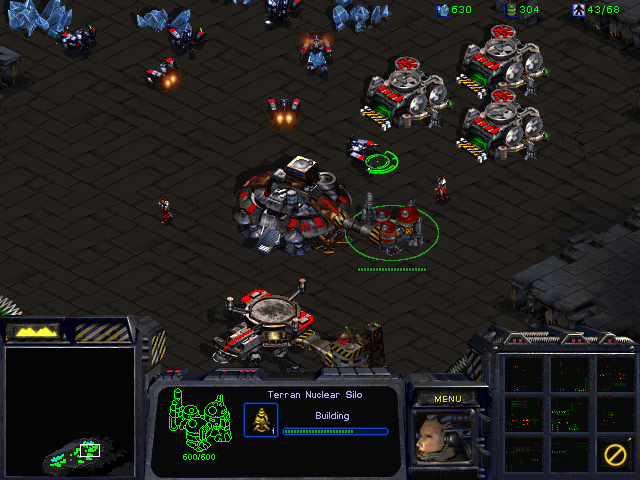
\includegraphics[scale=0.6]{media/starcraft-nuclear-silo.png}
	\caption{``Nuclear Sylow''.}
\end{figure}


Sylow's theorem is really huge for classifying groups;
in particular, the conditions $n_p \equiv 1 \pmod p$ and $n_p \mid m$
can often pin down the value of $n_p$ to just a few values.
Here are some results which follow from the Sylow theorems.
\begin{itemize}
	\ii A Sylow $p$-subgroup is normal if and only if $n_p = 1$.
	\ii Any group $G$ of order $pq$, where $p < q$ are primes,
	must have $n_q = 1$, since $n_q \equiv 1 \pmod q$ yet $n_q \mid p$.
	Thus $G$ has a normal subgroup of order $q$.
	\ii Since any abelian group has all subgroups normal,
	it follows that any abelian group has exactly one Sylow $p$-subgroup
	for every $p$ dividing its order.
	\ii If $p \neq q$, the intersection of a Sylow $p$-subgroup and a Sylow $q$-subgroup is just $\{1_G\}$.
	That's because the intersection of any two subgroups is also a subgroup,
	and Lagrange's theorem tells us that its order must divide both a power of $p$
	and a power of $q$; this can only happen if the subgroup is trivial.
\end{itemize}

Here's an example of another ``practical'' application.
\begin{proposition}[Triple product of primes]
	If $\left\lvert G \right\rvert = pqr$ is the product of distinct primes,
	then $G$ must have a normal Sylow subgroup.
\end{proposition}
\begin{proof}
	WLOG, assume $p<q<r$.  Notice that $n_p \equiv 1 \pmod p$, $n_p | qr$ and cyclically, and assume for contradiction that $n_p, n_q, n_r > 1$.
	
	Since $n_r | pq$, we have $n_r = pq$ since $n_r$ divides neither $p$ nor $q$ as $n_r \ge 1 + r > p,q$.  Also, $n_p \ge 1+p$ and $n_q \ge 1+q$.
	So we must have at least $1+p$ Sylow $p$-subgroups,
	at least $1+q$ Sylow $q$-subgroups, and at least $pq$ Sylow $r$-subgroups.

	But these groups are pretty exclusive.
	\begin{ques}
		Take the $n_p+n_q+n_r$ Sylow subgroups and consider two of them, 
		say $H_1$ and $H_2$.
		Show that $\left\lvert H_1 \cap H_2 \right\rvert = 1$
		as follows:
		check that $H_1 \cap H_2$ is a subgroup of both $H_1$ and $H_2$,
		and then use Lagrange's theorem.
	\end{ques}

	We claim that there are too many elements now.
	Indeed, if we count the non-identity elements contributed by these subgroups, we get
	\[ n_p(p-1) + n_q(q-1) + n_r(r-1)
		\ge (1+p)(p-1) + (1+q)(q-1) + pq(r-1) > pqr 
	\]
	which is more elements than $\left\lvert G \right\rvert$ has!
\end{proof}


\section{(Optional) Proving Sylow's theorem}
The proof of Sylow's theorem is somewhat involved,
and in fact many proofs exist.  I'll present one below here.
It makes extensive use of group actions,
so I want to recall the following facts first.
If $G$ acts on $X$, then
\begin{itemize}
	\ii The orbits of the action form a partition of $X$.
	\ii if $\OO$ is any orbit, then the orbit-Stabilizer theorem says that
	\[ \left\lvert \OO \right\rvert = \left\lvert G \right\rvert / \left\lvert \Stab_G(x) \right\rvert \]
	for any $x \in \OO$.
	\ii In particular: suppose in the above that $G$ is a group of order $p^t$.
	Then either $\left\lvert \OO \right\rvert = 1$ or $p$ divides $\left\lvert \OO \right\rvert$.
	In the case $\OO = \{x\}$, then by definition, $x$ is a \vocab{fixed point} of every element of $G$: we have $g \cdot x = x$ for every $x$.
\end{itemize}
Note that when I say $x$ is a fixed point, I mean it is fixed by \textbf{every} element of the group, i.e.\ the orbit really has size one. Hence that's a really strong condition.

\subsection*{Definitions}
\prototype{Conjugacy in$S_n$}
In addition, I need the following definitions.
I've defined conjugacy of elements previously,
but I now need to define it for groups:
\begin{definition}
	Let $G$ be a group, and let $X$ denote the set of subgroups of $G$.
	Then \vocab{conjugation} is the action of $G$ on $X$ that sends
	\[ H \mapsto gHg\inv = \left\{ ghg\inv \mid h \in H \right\}. \]
	If $H$ and $K$ are subgroups of $G$ such that $H = gKg\inv$ for some $g \in G$
	(in other words, they are in the same orbit under this action),
	then we say they are \vocab{conjugate} subgroups.
\end{definition}

Because we somehow don't think of conjugate elements as
``that different'' (for example, in permutation groups),
the following shouldn't be surprising.
\begin{ques}
	Show that for any subgroup $H$ of a group $G$, the map $H \to gHg\inv$ by
	$h \mapsto ghg\inv$ is in fact an isomorphism.
	This implies that any two conjugate subgroups are isomorphic.
\end{ques}

\begin{definition}
	For any subgroup $H$ of $G$ the \vocab{normalizer} of $H$ is defined as
	\[ N_G(H) \defeq \left\{ g \in G \mid gHg\inv = H \right\}. \]
	In other words, it is the stabilizer of $H$ under the conjugation action.
\end{definition}

We are now ready to present the proof.

\subsection*{Step 1: Prove that a Sylow $p$-subgroup exists}
What follows is something like the probabilistic method.
By considering the set $X$ of ALL subsets of size $p^n$ at once, we can exploit the ``deep number theoretic fact'' that 
\[ \left\lvert X \right\rvert = \binom{p^n m}{p^n} \not\equiv 0 \pmod p. \]
(It's not actually deep: use Lucas' theorem.)

Here is the proof.
\begin{itemize}
	\ii Let $G$ act on $X$ by $g \cdot X \defeq \left\{ gx \mid x \in X \right\}$.
	\ii Take an orbit $\OO$ with size not divisible by $p$.
	(This is possible because of our deep number theoretic fact.
	Since $\left\lvert X \right\rvert$ is nonzero mod $p$ and the orbits partition $X$, the claimed orbit must exist. )
	\ii let $S \in \OO$, $H = \Stab_G(S)$. then $p^n$ divides $\left\lvert H \right\rvert$, by the orbit-Stabilizer theorem.
	\ii Consider a second action: let $H$ act on $S$ by 
	$h \cdot s \defeq hs$ (we know $hs \in S$ since $H = \Stab_G(S)$).
	\ii
	Observe that $\Stab_H(s) = \{1_H\}$.
	Then all orbits of the second action must have size $\left\lvert H \right\rvert$. Thus $\left\lvert H \right\rvert$ divides $\left\lvert S \right\rvert = p^n$.
	\ii This implies $\left\lvert H \right\rvert = p^n$, and we're done.
\end{itemize}


\subsection*{Step 2: Any two Sylow $p$-subgroups are conjugate}
Let $P$ be a Sylow $p$-subgroup (which exists by the previous step).
We now prove that for any $p$-group $Q$, $Q \subseteq gPg\inv$.
Note that if $Q$ is also a Sylow $p$-subgroup, then $Q = gPg\inv$ for size reasons;
this implies that any two Sylow subgroups are indeed conjugate.

\textbf{Let $Q$ act on the set of left cosets of $P$ by left multiplication.}
Note that
\begin{itemize}
	\ii $Q$ is a $p$-group, so any orbit has size divisible by $p$ unless it's $1$.
	\ii But the number of left cosets is $m$, which isn't divisible by $p$.
\end{itemize}
\textbf{Hence some coset $gP$ is a fixed point for every $q$}, meaning
$qgP = gP$ for all $q$.
Equivalently, $qg \in gP$ for all $q \in Q$, so $Q \subseteq gPg\inv$ as desired.


\subsection*{Step 3: Showing $n_p \equiv 1 \pmod p$}
Let $\mathcal S$ denote the set of all the Sylow $p$-subgroups.
Let $P \in \mathcal S$ be arbitrary.
\begin{ques}
	Why does $\left\lvert \mathcal S \right\rvert$ equal $n_p$?
	(In other words, are you awake?)
\end{ques}
Now we can proceed with the proof.
Let $P$ act on $\mathcal S$ by conjugation.
Then:
\begin{itemize}
	\ii Because $P$ is a $p$-group, $n_p \pmod p$ is the number of fixed points
	of this action.
	Now we claim $P$ is the only fixed point of this action.
	\ii Let $Q$ be any other fixed point, meaning $xQx\inv = Q$ for any $x \in G$.
	\ii Define the normalizer $N_G(Q) = \left\{ g \in G \mid gQg\inv = Q \right\}$.  It contains both $P$ and $Q$.
	\ii Now for the crazy part: apply Step 2 to $N_G(Q)$.
	Since $P$ and $Q$ are Sylow $p$-subgroups of it, they must be conjugate.
	\ii Hence $P=Q$, as desired.
\end{itemize}

\subsection*{Step 4: $n_p$ divides $m$}
Since $n_p \equiv 1 \pmod p$, it suffices to show $n_p$ divides $\left\lvert G \right\rvert$.
Let $G$ act on the set of all Sylow $p$-groups by conjugation.
Step 2 says this action has only one orbit, so the Orbit-Stabilizer theorem
implies $n_p$ divides $\left\lvert G \right\rvert$.


\section{(Optional) Simple groups and Jordan-H\"older}
\prototype{Decomposition of $\Zc{12}$ is $1 \normalin \Zc 2 \normalin \Zc 4 \normalin \Zc{12}$.}
% Fortunately, there is at least a way to ``break down'' $G$.
Just like every integer breaks down as the product of primes,
we can try to break every group down as a product of ``basic'' groups.
Armed with our idea of quotient groups, the right notion is this.

\begin{definition}
	A \vocab{simple group} is a group with no normal subgroups
	other than itself and the trivial group.
\end{definition}
\begin{ques}
	For which $n$ is $\Zc n$ simple? (Hint: remember that $\Zc n$ is abelian.)
\end{ques}

\begin{figure}[ht]
	\centering
	\snsd[height=7cm]{my-world-symmetric-group.png}
	\caption{The group $S_n$ is simple when $n=2$. Also, Google ``solvable groups''.}
\end{figure}


Then we can try to define what it means to ``break down a group''.
\begin{definition}
	A \vocab{composition series} of a group $G$ is a sequence of subgroups
	$H_0$, $H_1$, \dots, $H_n$ such that
	\[ \{1\} = H_0 \normalin H_1 \normalin H_2 \normalin \dots \normalin H_n
		\normalin G \]
	of maximal length (i.e.\ $n$ is as large as possible).
	The \vocab{composition factors} are the groups
	$H_1/H_0$, $H_2/H_1$, \dots, $H_n/H_{n-1}$.
\end{definition}
You can show that the ``maximality'' condition implies that the composition factors are all simple groups.

Let's say two composition series are equivalent if they have the same composition factors (up to permutation); in particular they have the same length.
Then it turns out that the following theorem \emph{is} true.
\begin{theorem}
	[Jordan-H\"older]
	Every finite group $G$ admits a unique composition series up to equivalence.
\end{theorem}

\begin{example}
	[Fundamental theorem of arithmetic when $n=12$]
	Let's consider the group $\Zc{12}$.
	It's not hard to check that the possible composition series are
	\begin{align*}
		\{1\} \normalin \Zc2 \normalin \Zc4 \normalin \Zc{12}
		& \text{ with factors $\Zc2$, $\Zc2$, $\Zc3$} \\
		\{1\} \normalin \Zc2 \normalin \Zc6 \normalin \Zc{12}
		& \text{ with factors $\Zc2$, $\Zc3$, $\Zc2$} \\
		\{1\} \normalin \Zc3 \normalin \Zc6 \normalin \Zc{12}
		& \text{ with factors $\Zc3$, $\Zc2$, $\Zc2$}.
	\end{align*}
	These correspond to the factorization $12 = 2^2 \cdot 3$.
\end{example}

This suggests that classifying all finite simple groups would be great progress, since every finite group is somehow a ``product'' of simple groups;
the only issue is that there are multiple ways of building a group from constituents.

Amazingly, we actually \emph{have} a full list of simple groups,
but the list is really bizarre.
Every finite simple group falls in one of the following categories:
\begin{itemize}
	\ii $\Zc p$ for $p$ a prime,
	\ii For $n \ge 5$, the subgroup of $S_n$ consisting of ``even'' permutations.
	\ii A simple group of Lie type (which I won't explain), and
	\ii Twenty-six ``sporadic'' groups which do not fit into any nice family.
\end{itemize}
The two largest of the sporadic groups have cute names.
The \vocab{baby monster group} has order 
\[ 2^{41} \cdot 3^{13} \cdot 5^6 \cdot 7^2 \cdot 11 \cdot 13 \cdot 17
	\cdot 19 \cdot 23 \cdot 31 \cdot 47 \approx 4 \cdot 10^{33} \]
and the \vocab{monster group} (also ``\vocab{friendly giant}'') has order
\[ 
	2^{46} \cdot 3^{20} \cdot 5^9 \cdot 7^6 \cdot 11^2 \cdot 13^3
	\cdot 17 \cdot 19 \cdot 23 \cdot 29 \cdot 31 \cdot 41 \cdot 47
	\cdot 59 \cdot 71 \approx 8 \cdot 10^{53}. \]
It contains twenty of the sporadic groups as subquotients (including itself),
and these twenty groups are called the ``\vocab{happy family}''.

\begin{figure}[ht]
	\centering
	\includegraphics[width=0.5\textwidth]{media/monster.jpg}
	\caption{On the topic of monsters\dots}
\end{figure}

Math is weird.

\begin{ques}
	Show that ``finite simple group of order $2$'' is redundant
	in the sense that any group of order $2$ is both finite and simple.
\end{ques}

\section\problemhead


\begin{sproblem}
	[Cauchy's theorem]
	Let $G$ be a group and let $p$ be a prime dividing $\left\lvert G \right\rvert$.
	Prove\footnote{
		Cauchy's theorem can be proved without the Sylow theorems,
		and in fact can often be used to give alternate proofs of Sylow.}
	that $G$ has an element of order $p$.
	\label{thm:cauchy_group}
\end{sproblem}

\begin{problem}
	Let $G$ be a finite simple group.
	Show that $\left\lvert G \right\rvert \neq 56$.
	\begin{hint}
		Count Sylow $8$ and $7$ groups and let them intersect.
	\end{hint}
	\begin{sol}
		If not, there exists eight Sylow $7$-groups and seven Sylow $8$-groups
		(since $n_7 \equiv 1 \pmod 7$, $n_8 \mid 7$, and $n_7, n_8 > 1$).
		But no two of thees $8+7=15$ groups can intersect at an element other than $1_G$,
		which is clearly absurd.
	\end{sol}
\end{problem}

\begin{problem}
	[Engel's PSS?]
	\gim
	Consider the set of all words consisting of the letters $a$ and $b$.
	Given such a word, we can change the word either by inserting a word of the form $www$,
	where $w$ is a word, anywhere in the given word, or by deleting such a sequence from the word.
	Can we turn the word $ab$ into the word $ba$?
	% http://www.artofproblemsolving.com/Forum/viewtopic.php?f=780&t=456603&p=2572053
	% lol Alex Zhu op
	\begin{hint}
		Construct a non-abelian group such that all elements have order three.
	\end{hint}
	\begin{sol}
		One example is upper triangular matrices with entries in mod $3$.
	\end{sol}
\end{problem}

\begin{problem}
	\yod
	Let $p$ be a prime.
	Show that the only simple group with order $p^n$
	(for some positive integer $n$)
	is the cyclic group $\Zc p$.

	% class equation
	\begin{hint}
		First, if $G$ abelian it's trivial.
		Otherwise, let $Z(G)$ be the center of the group,
		which is always a normal subgroup of $G$.
		Do a mod $p$ argument via conjugation (or use the class equation).
	\end{hint}
	\begin{sol}
		Let $G$ be said group.
		If $G$ is abelian then all subgroups are normal,
		and since $G$ is simple, $G$ can't have any subgroups at all.
		We can clearly find an element of order $p$, hence $G$ has a subgroup
		of order $p$, which can only happen if $n=1$, $G \cong \Zc p$.

		Thus it suffices to show $G$ can't be abelian.
		For this, we can use the class equation, but let's avoid that and do it directly:

		Assume not and let $Z(G) = \{ g \in G \mid xg = gx \; \forall x \in G \}$
		be the center of the group.
		Since $Z(G)$ is normal in $G$, and $G$ is simple, we see $Z(G) = \{1_G\}$.
		But then let $G$ act on itself by conjugation: $g \cdot x = gxg\inv$.
		This breaks $G$ into a bunch of orbits $\OO_0 = \{1_G\}$, $\OO_1$, $\OO_2$, \dots,
		and since $1_G$ is the only fixed point by definition, all other orbits
		have size greater than $1$.
		The Orbit-stabilizer theorem says that each orbit now has size dividing $p^n$,
		so they must all have size zero mod $p$.

		But then summing across all orbits (which partition $G$),
		we obtain $\left\lvert G \right\rvert \equiv 1 \pmod p$,
		which is a contradiction.
	\end{sol}
\end{problem}


\endinput

%\section{Semidirect Products}
%\prototype{$D_{12} \cong C_6 \rtimes C_2$.}
%(Semidirect products are a little heavy and I won't use them other than to illustrate a point in this section.
%So you might skip this section on a first read.)
%
%Let $G$ be a group and $N$ a normal subgroup.
%Let $Q = G/N$.
%Is there a way we can recover $G$ as a ``product'' of $Q$ and $N$?
%
%Our first guess would be $G \cong N \times Q$, the Cartesian product.
%Unfortunately, this fails.
%For example, let $G = D_{12}$, and let $N = \left\{ 1,r,\dots,r^5 \right\}$.
%You can check that $N$ is indeed normal in $D_{12}$; however, $D_{12}/N \cong C_2$ while $N \cong C_6$.
%And it's certainly not the case that $D_{12} \cong C_6 \times C_2$, since
%$D_{12}$ is not abelian!
%
%In fact, we have that
%\[ C_{12} / C_6 \cong C_2 \text{ and } D_{12} / C_6 \cong C_2 \]
%so we can't even determine $G$ uniquely.
%But can we at least find all possible $G$?
%
%You can define another type of product, called a semidirect product, as follows.
%\begin{definition}
%	An \vocab{automorphism} is an isomorphism from a group to itself.
%	Given a group $G$, let $\Aut(G)$ be the set of automorphisms of $G$.
%	Then $\Aut(G)$ forms a group, called the \vocab{automorphism group} of $G$.
%\end{definition}
%\begin{definition}
%	Let $H = (H, \star)$ and $K = (K, \ast)$ be groups.
%	Let $\phi : K \to \opname{Aut}(H)$ be a homomorphism.
%	Then we define the \vocab{semidirect product} $H \rtimes_\phi K$ as follows.
%	\begin{itemize}
%		\ii The elements of $H \rtimes K$ are ordered pairs $(h,k) \in H \times K$.
%		\ii The group operation will be
%		\[ (h_1, k_1)(h_2, k_2)
%			= \left( h_1 \star \phi_{k_1}(h_2), k_1 \ast k_2 \right). \]
%	\end{itemize}
%\end{definition}
%In the above, I've let $\phi_k$ denote the image of $k \in K$ under $\phi$.
%It's not hard to check that this actually makes $H \rtimes_\phi K$ into a group.
%\begin{ques}
%	Convince yourself that $H' = \left\{ (1,k) \mid k \in K \right\}$
%	is a subgroup of $H \rtimes_\phi K$ which is isomorphic to $H$.
%	Also, show that $H' \normalin H \rtimes_\phi K$.
%\end{ques}
%\begin{example}[Dihedral Group]
%	Let $H = C_n = \left<x \mid x^n=1\right>$ and $K = C_2 = \left<y \mid y^2=1\right>$.
%	Let $\phi : C_2 \to \Aut(C_n)$ by sending $x$ to the map $y \mapsto y\inv$.
%	In other words, $\phi_x(y) = y\inv$.
%	Then \[ D_{2n} = C_n \rtimes_\phi C_2. \]
%\end{example}
%
%Unfortunately, even this isn't enough to capture all possible values of $G$.
%This only works if there's a natural way that you can view $K$ as a subgroup of $G$, since this construction also causes $K$ to appear as a subgroup of $G$.
%Alas, this is not always possible.

\chapter{Rings and ideals}
\section{Some motivational metaphors about rings vs groups}
In this chapter we'll introduce the notion of
a \textbf{commutative ring} $R$.
It is a larger structure than a group:
it will have two operations addition and multiplication,
rather than just one.
We will then immediately define a \textbf{ring homomorphism}
$R \to S$ between pairs of rings.

This time, instead of having normal subgroups $H \normalin G$,
rings will instead have subsets $I \subseteq R$ called \textbf{ideals},
which are not themselves rings but satisfy some niceness conditions.
We will then show how you to define $R/I$,
in analogy to $G/H$ as before.
Finally, like with groups, we will talk a bit about how to generate ideals.

Here is a possibly helpful table of analogies to help you keep track:
\begin{center}
	\begin{tabular}[h]{lcc}
		& Group & Ring \\
		\hline
		Notation & $G$ & $R$ \\
		Operations & $\cdot$ & $+$, $\times$ \\
		Commutativity & only if abelian & for us, always \\
		Sub-structure & subgroup & (not discussed) \\
		Homomorphism & grp hom.\ $G \to H$ & ring hom.\ $R \to S$ \\
		Kernel & normal subgroup & ideal \\
		Quotient & $G/H$ & $R/I$ \\
	\end{tabular}
\end{center}

\section{(Optional) Pedagogical notes on motivation}
I wrote most of these examples with a number theoretic eye in mind;
thus if you liked elementary number theory,
a lot of your intuition will carry over.
Basically, we'll try to generalize properties of the ring $\ZZ$ to
any abelian structure in which we can also multiply.
That's why, for example, you can talk about
``irreducible polynomials in $\QQ[x]$'' in the same
way you can talk about ``primes in $\ZZ$'',
or about ``factoring polynomials modulo $p$''
in the same way we can talk ``unique factorization in $\ZZ$''.
Even if you only care about $\ZZ$
(say, you're a number theorist), this has a lot of value:
I assure you that trying to solve $x^n+y^n = z^n$ (for $n > 2$)
requires going into a ring other than $\ZZ$!

Thus for all the sections that follow, keep $\ZZ$ in mind as your prototype.

I mention this here because
commutative algebra is \emph{also} closely tied to algebraic geometry.
Lots of the ideas in commutative algebra have nice
``geometric'' interpretations that motivate the definitions,
and these connections are explored in the corresponding part later.
So, I want to admit outright that this is not
the only good way (perhaps not even the most natural one)
of motivating what is to follow.

\section{Definition and examples of rings}
\prototype{$\ZZ$ all the way! Also $R[x]$ and various fields (next section).}

Well, I guess I'll define a ring\footnote{Or,
	according to some authors, a ``ring with identity'';
	some authors don't require rings to have multiplicative identity.
	For us, ``ring'' always means ``ring with $1$''.}.

\begin{definition}
	A \vocab{ring} is a triple $(R, +, \times)$,
	the two operations usually called addition and multiplication, such that
	\begin{enumerate}[(i)]
		\ii $(R,+)$ is an abelian group, with identity $0_R$, or just $0$.
		\ii $\times$ is an associative, binary operation on $R$ with some
		identity, written $1_R$ or just $1$.
		\ii Multiplication distributes over addition.
	\end{enumerate}
	The ring $R$ is \vocab{commutative} if $\times$ is commutative.
\end{definition}
\begin{abuse}
	As usual, we will abbreviate $(R, +, \times)$ to $R$.
\end{abuse}
\begin{abuse}
	For simplicity, assume all rings are commutative
	for the rest of this chapter.
	We'll run into some noncommutative rings eventually,
	but for such rings we won't need the full theory of this chapter anyways.
\end{abuse}

These definitions are just here for completeness.
The examples are much more important.
\begin{example}[Typical rings]
	\listhack
	\begin{enumerate}[(a)]
		\ii The sets $\ZZ$, $\QQ$, $\RR$ and $\CC$ are all rings
		with the usual addition and multiplication.
		\ii The integers modulo $n$ are also a ring
		with the usual addition and multiplication.
		We also denote it by $\Zc n$.
	\end{enumerate}
\end{example}

Here is also a trivial example.
\begin{definition}
	The \vocab{zero ring} is the ring $R$ with a single element.
	We denote the zero ring by $0$.
	A ring is \vocab{nontrivial} if it is not the zero ring.
\end{definition}
\begin{exercise}
	[Comedic]
	Show that a ring is nontrivial if and only if $0_R \ne 1_R$.
\end{exercise}

Since I've defined this structure, I may as well state the obligatory facts about it.
\begin{fact}
	For any ring $R$ and $r \in R$, $r \cdot 0_R = 0_R$.
	Moreover, $r \cdot (-1_R) = -r$.
\end{fact}

Here are some more examples of rings.
\begin{example}
	[Product ring]
	\label{ex:product_ring}
	Given two rings $R$ and $S$ the \vocab{product ring},
	denoted $R \times S$, is defined as ordered pairs $(r,s)$
	with both operations done component-wise.
	For example, the Chinese remainder theorem says
	that \[ \Zc{15} \cong \Zc3 \times \Zc5 \]
	with the isomorphism $n \bmod{15} \mapsto (n \bmod 3, n \bmod 5)$.
\end{example}
\begin{remark}
	Equivalently, we can define $R \times S$ as the abelian group $R \oplus S$,
	and endow it with the multiplication where $r \cdot s = 0$
	for $r \in R$, $s \in S$.
\end{remark}
\begin{ques}
	Which $(r,s)$ is the identity element of the product ring $R \times S$?
\end{ques}

\begin{example}[Polynomial ring]
	Given any ring $R$,
	the \vocab{polynomial ring} $R[x]$ is defined as the set of polynomials
	with coefficients in $R$:
	\[ R[x] = \left\{ a_n x^n+a_{n-1}x^{n-1}+\dots+a_0
		\mid a_0, \dots, a_n \in R \right\}. \]
	This is pronounced ``$R$ adjoin $x$''.
	Addition and multiplication are done exactly in the way you would expect.
\end{example}
\begin{remark}
	[Digression on division]
	Happily, polynomial division also does what we expect:
	if $p(x) \in R[x]$ and $p(a) = 0$,
	then $(x-a)q(x) = p(x)$ for some polynomial $q$.
	Proof: do polynomial long division.
	With that, note the caveat that
	\[ x^2-1 \equiv (x-1)(x+1) \pmod 8 \]
	has \emph{four} roots $1$, $3$, $5$, $7$ in $\Zc8$.

	The problem is that $2 \cdot 4 = 0$ even though $2$ and $4$ are not zero;
	we call $2$ and $4$ \emph{zero divisors} for that reason.
	In an \emph{integral domain} (a ring without zero divisors),
	this pathology goes away,
	and just about everything you know about polynomials carries over.
	(I'll say this all again next section.)
\end{remark}
\begin{example}
	[Multi-variable polynomial ring]
	We can consider polynomials in $n$ variables with coefficients in $R$,
	denoted $R[x_1, \dots, x_n]$.
	(We can even adjoin infinitely many $x$'s if we like!)
\end{example}

\begin{example}
	[Gaussian integers are a ring]
	The \vocab{Gaussian integers} are the set of complex numbers
	with integer real and imaginary parts, that is
	\[ \ZZ[i] = \left\{ a+bi \mid a,b \in \ZZ \right\}. \]
\end{example}
\begin{abuse}
	[Liberal use of adjoinment]
	Extremely careful readers will detect some abuse in notation here.
	$\ZZ[i]$ should officially be
	``integer-coefficient polynomials in $i$''.
	However, as $i^2=-1$, a polynomial in $i$ is the same as
	a Gaussian integer. So not a big deal.
\end{abuse}
\begin{example}
	[Cube root of $2$]
	As another example:
	\[ \ZZ[\sqrt[3]{2}] = \left\{ a + b\sqrt[3]{2} + c\sqrt[3]4
		\mid a,b,c \in \ZZ \right\}. \]
\end{example}

\section{Fields}
\prototype{$\QQ$ is a field, but $\ZZ$ is not.}

Although we won't need to know what a field is until next chapter,
they're so convenient for examples I will go ahead and introduce them now.

As you might already know, if the multiplication is invertible,
then we call the ring a field.
To be explicit, let me write the relevant definitions.

\begin{definition}
	\label{def:unit}
	A \vocab{unit} of a ring $R$
	is an element $u \in R$ which is invertible:
	for some $x \in R$ we have $ux = 1_R$.
\end{definition}

\begin{example}
	[Examples of units]
	\listhack
	\begin{enumerate}[(a)]
	\ii The units of $\ZZ$ are $\pm 1$,
	because these are the only things which ``divide $1$''
	(which is the reason for the name ``unit'').
	\ii On the other hand, in $\QQ$ everything is a unit (except $0$).
	For example, $\frac 35$ is a unit since
	$\frac 35 \cdot \frac 53 = 1$.
	\ii The Gaussian integers $\ZZ[i]$ have four units:
	$\pm 1$ and $\pm i$.
	\end{enumerate}
\end{example}

\begin{definition}
	A nontrivial (commutative) ring is a \vocab{field}
	when all its nonzero elements are units.
\end{definition}

Colloquially, we say that
\begin{moral}
	A field is a structure where you can add, subtract, multiply, and divide.
\end{moral}
Depending on context, they are often denoted
either $k$, $K$, $F$.

\begin{example}
	[First examples of fields]
	\listhack
	\begin{enumerate}[(a)]
		\ii $\QQ$, $\RR$, $\CC$ are fields,
		since the notion $\frac 1c$ makes sense in them.
		\ii If $p$ is a prime, then $\Zc p$ is a field,
		which we denote will usually denote by $\FF_p$.
	\end{enumerate}
	The trivial ring $0$ is \emph{not} considered a field,
	since we require fields to be nontrivial.
\end{example}

%\begin{remark}
%	You might say at this point that ``fields are nicer than rings'',
%	but as you'll see in this chapter, the conditions for
%	being a field are somehow ``too strong''.
%	To give an example of what I mean:
%	if you try to think about the concept of ``divisibility''
%	in $\ZZ$, you've stepped into the vast and bizarre realm of
%	number theory.  Try to do the same thing in $\QQ$ and you get nothing:
%	any nonzero $a$ ``divides'' any nonzero $b$
%	because $b = a \cdot \frac ba$.
%
%	I know at least one person who instead
%	thinks of this as an argument for why people
%	shouldn't care about number theory
%	(studying chaos rather than order).
%\end{remark}

\section{Homomorphisms}
\prototype{$\ZZ \to \Zc5$ by modding out by $5$.}
This section is going to go briskly --
it's the obvious generalization of all the stuff
we did with quotient groups.\footnote{I once found an
	abstract algebra textbook which teaches rings before groups.
	At the time I didn't understand why,
	but now I think I get it -- modding out by things in
	commutative rings is far more natural, and you can start talking
	about all the various flavors of rings and fields.
	You also have (in my opinion) more vivid first examples
	for rings than for groups.
	I actually sympathize a lot with this approach --- maybe I'll convert
	Napkin to follow it one day.}

First, we define a homomorphism and isomorphism.
\begin{definition}
	Let $R = (R, +_R, \times_R)$ and $S = (S, +_S, \times_S)$ be rings.
	A \vocab{ring homomorphism} is a map $\phi : R \to S$
	such that 
	\begin{enumerate}[(i)]
		\ii $\phi(x +_R y) = \phi(x) +_S \phi(y)$ for each $x,y \in R$.
		\ii $\phi(x \times_R y) = \phi(x) \times_S \phi(y)$ for each $x,y \in R$.
		\ii $\phi(1_R) = 1_S$.
	\end{enumerate}
	If $\phi$ is a bijection then $\phi$ is an \vocab{isomorphism}
	and we say that rings $R$ and $S$ are \vocab{isomorphic}.
\end{definition}
Just what you would expect.
The only surprise is that we also demand $\phi(1_R)$ to go to $1_S$.
This condition is not extraneous:
consider the map $\ZZ \to \ZZ$ called ``multiply by zero''.
\begin{example}
	[Examples of homomorphisms]
	\listhack
	\begin{enumerate}[(a)]
		\ii The identity map, as always.
		\ii The map $\ZZ \to \Zc5$ modding out by $5$.
		\ii The map $\RR[x] \to \RR$ by $p(x) \mapsto p(0)$
		by taking the constant term.
		\ii For any ring $R$, there is a trivial ring homomorphism $R \to 0$.
	\end{enumerate}
\end{example}
\begin{example}
	[Non-examples of homomorphisms]
	Because we require $1_R$ to $1_S$, some maps that you
	might have thought were homomorphisms will fail.
	\begin{enumerate}[(a)]
		\ii The map $\ZZ \to \ZZ$ by $x \mapsto 2x$
		is not a ring homomomorphism.
		Aside from the fact it sends $1$ to $2$,
		it also does not preserve multiplication.

		\ii If $S$ is a nontrivial ring,
		the map $R \to S$ by $x \mapsto 0$ is not
		a ring homomorphism, even though it preserves multiplication.

		\ii There is no ring homomorphism $\Zc{2016} \to \ZZ$ at all.
	\end{enumerate}
	In particular, whereas for groups $G$ and $H$
	there was always a trivial group homomorphism sending
	everything in $G$ to $1_H$, this is not the case for rings.
\end{example}

\section{Ideals}
\prototype{The multiples of $5$ are an ideal of $\ZZ$.}
Now, just like we were able to mod out by groups,
we'd also like to define quotient rings.
So once again,
\begin{definition}
	The \vocab{kernel} of a ring homomorphism $\phi \colon R \to S$,
	denoted $\ker \phi$, is the set of $r \in R$ such that $\phi(r) = 0$.
\end{definition}

In group theory, we were able to characterize the ``normal'' subgroups by a few
obviously necessary conditions (namely, $gHg\inv = H$).
We can do the same thing for rings, and it's in fact easier because our operations are commutative.

First, note two obvious facts:
\begin{itemize}
	\ii If $\phi(x) = \phi(y) = 0$, then $\phi(x+y) = 0$ as well.
	So $\ker \phi$ should be closed under addition.
	\ii If $\phi(x) = 0$, then for any $r \in R$ we have
	$\phi(rx) = \phi(r)\phi(x) = 0$ too.
	So for $x \in \ker \phi$ and \emph{any} $r \in R$,
	we have $rx \in \ker\phi$.
\end{itemize}

A (nonempty) subset $I \subseteq R$ is called
an ideal if it satisfies these properties.
That is,
\begin{definition}
	A nonempty subset $I \subseteq R$ is an \vocab{ideal}
	if it is closed under addition, and for each $x \in I$,
	$rx \in I$ for all $r \in R$.
	It is \vocab{proper} if $I \neq R$.
\end{definition}

Note that in the second condition, $r$ need not be in $I$!
So this is stronger than merely saying $I$ is closed under multiplication.
\begin{remark}
	If $R$ is not commutative, we also need the condition $xr \in I$.
	That is, the ideal is \emph{two-sided}: it absorbs multiplication
	from both the left and the right.
	But since rings in Napkin are commutative
	we needn't worry with this distinction.
\end{remark}

\begin{example}
	[Prototypical example of an ideal]
	Consider the set $I = 5\ZZ = \{\dots,-10,-5,0,5,10,\dots\}$ as an ideal in $\ZZ$.
	We indeed see $I$ is the kernel of the ``take mod $5$'' homomorphism:
	\[ \ZZ \surjto \ZZ/5\ZZ. \]
	It's clearly closed under addition,
	but it absorbs multiplication from \emph{all} elements of $\ZZ$:
	given $15 \in I$, $999 \in \ZZ$, we get $15 \cdot 999 \in I$.
\end{example}

\begin{exercise}
	[Mandatory: fields have two ideals]
	If $K$ is a field, show that $K$ has exactly two ideals.
	What are they?
	\label{exer:field_ideal}
\end{exercise}

Now we claim that these conditions are sufficient.
More explicitly,
\begin{theorem}
	[Ring analog of normal subgroups]
	Let $R$ be a ring and $I \subsetneq R$.
	Then $I$ is the kernel of some homomorphism if and only if it's an ideal.
\end{theorem}
\begin{proof}
	It's quite similar to the proof for the normal subgroup thing,
	and you might try it yourself as an exercise.
	
	Obviously the conditions are necessary.
	To see they're sufficient, we \emph{define} a ring by ``cosets''
	\[ S = \left\{ r + I \mid r \in R \right\}. \]
	These are the equivalence where we say $r_1 \sim r_2$ if $r_1 - r_2 \in I$
	(think of this as taking ``mod $I$'').
	To see that these form a ring, we have to check that the addition
	and multiplication we put on them is well-defined.
	Specifically, we want to check that if $r_1 \sim s_1$ and $r_2 \sim s_2$,
	then $r_1 + r_2 \sim s_1 + s_2$ and $r_1r_2 \sim s_1s_2$.
	We actually already did the first part
	-- just think of $R$ and $S$ as abelian
	groups, forgetting for the moment that we can multiply.
	The multiplication is more interesting.
	\begin{exercise}
		[Recommended]
		Show that if $r_1 \sim s_1$ and $r_2 \sim s_2$, then $r_1r_2 \sim s_1s_2$.
		You will need to use the fact that $I$ absorbs multiplication
		from \emph{any} elements of $R$, not just those in $I$.
	\end{exercise}
	Anyways, since this addition and multiplication is well-defined there
	is now a surjective homomorphism $R \to S$ with kernel exactly $I$.
\end{proof}

\begin{definition}
	Given an ideal $I$, we define as above the \vocab{quotient ring}
	\[ R/I \defeq \left\{ r+I \mid r \in R \right\}. \]
	It's the ring of these equivalence classes.
	This ring is pronounced ``$R$ mod $I$''.
\end{definition}
\begin{example}[$\ZZ/5\ZZ$]
	The integers modulo $5$ formed by ``modding out additively by $5$''
	are the $\Zc 5$ we have already met.
\end{example}
But here's an important point:
just as we don't actually think of $\ZZ/5\ZZ$ as consisting of
$k + 5\ZZ$ for $k=0,\dots,4$,
we also don't really want to think about $R/I$ as elements $r+I$.
The better way to think about it is
\begin{moral}
	$R/I$ is the result when we declare that elements of $I$ are all zero;
	that is, we ``mod out by elements of $I$''.
\end{moral}
For example, modding out by $5\ZZ$ means that we consider
all elements in $\ZZ$ divisible by $5$ to be zero.
This gives you the usual modular arithmetic!

\section{Generating ideals}
\prototype{In $\ZZ$, the ideals are all of the form $(n)$.}

Let's give you some practice with ideals.

An important piece of intuition is that once an ideal
contains a unit, it contains $1$, and
thus must contain the entire ring.
That's why the notion of ``proper ideal''
is useful language.
To expand on that:
\begin{proposition}
	[Proper ideal $\iff$ no units]
	Let $R$ be a ring and $I \subseteq R$ an ideal.
	Then $I$ is proper (i.e.\ $I \ne R$)
	if and only if it contains no units of $R$.
\end{proposition}
\begin{proof}
	Suppose $I$ contains a unit $u$, i.e.\ an element $u$
	with an inverse $u\inv$.
	Then it contains $u \cdot u\inv = 1$, and thus $I = R$.
	Conversely, if $I$ contains no units, it is obviously proper.
\end{proof}
As a consequence, if $K$ is a field,
then its only ideals are $(0)$ and $K$
(this was \Cref{exer:field_ideal}).
So for our practice purposes, we'll be working with rings that aren't fields.

First practice: $\ZZ$.
\begin{exercise}
	Show that the only ideals of $\ZZ$ are precisely those
	sets of the form $n\ZZ$, where $n$ is a nonnegative integer.
\end{exercise}

Thus, while ideals of fields are not terribly interesting,
ideals of $\ZZ$ look eerily like elements of $\ZZ$.
Let's make this more precise.
\begin{definition}
	Let $R$ be a ring.
	The \vocab{ideal generated} by a set of elements $x_1, \dots, x_n \in R$
	is denoted by $I = (x_1, x_2, \dots, x_n)$
	and given by
	\[ I = \left\{ r_1 x_1 + \dots + r_n x_n \mid r_i \in R \right\}.  \]
	One can think of this as ``the smallest ideal containing all the $x_i$''.
\end{definition}

The analogy of putting the $\{x_i\}$ in a sealed box and shaking vigorously
kind of works here too.
\begin{remark}
	[Linear algebra digression]
	If you know linear algebra,
	you can summarize this as: an ideal is an $R$-module.
	The ideal $(x_1, \dots, x_n)$ is the submodule spanned by $x_1, \dots, x_n$.
\end{remark}

In particular, if $I = (x)$ then $I$ consists of exactly the
``multiples of $x$'', i.e.\ numbers of the form $rx$ for $r \in R$.
\begin{remark}
	We can also apply this definition to infinite generating sets,
	as long as only finitely many of the $r_i$ are not zero
	(since infinite sums don't make sense in general).
\end{remark}

\begin{example}[Examples of generated ideals]
	\listhack
	\begin{enumerate}[(a)]
		\ii As $(n) = n\ZZ$ for all $ \in \ZZ$,
		every ideal in $\ZZ$ is of the form $(n)$.
		\ii In $\ZZ[i]$, we have
		$(5) = \left\{ 5a + 5b i \mid a,b \in \ZZ \right\}$.
		\ii In $\ZZ[x]$, the ideal $(x)$ consists of polynomials
		with zero constant terms.
		\ii In $\ZZ[x,y]$, the ideal $(x,y)$ again consists
		of polynomials with zero constant terms.
		\ii In $\ZZ[x]$, the ideal $(x,5)$ consists of polynomials
		whose constant term is divisible by $5$.
	\end{enumerate}
\end{example}
\begin{ques}
	Please check that the set
	$I = \left\{ r_1 x_1 + \dots + r_n x_n \mid r_i \in R \right\}$
	is indeed always an ideal (closed under addition,
	and absorbs multiplication).
\end{ques}
Now suppose $I = (x_1, \dots, x_n)$.
What does $R/I$ look like?
According to what I said at the end of the last section,
it's what happens when we ``mod out'' by each of the elements $x_i$.
For example\dots
\begin{example}
	[Modding out by generated ideals]
	\listhack
	\begin{enumerate}[(a)]
		\ii Let $R = \ZZ$ and $I = (5)$. Then $R/I$ is literally
		$\ZZ/5\ZZ$, or the ``integers modulo $5$'':
		it is the result of declaring $5 = 0$.
		\ii Let $R = \ZZ[x]$ and $I = (x)$.
		Then $R/I$ means we send $x$ to zero; hence $R/I \cong \ZZ$
		as given any polynomial $p(x) \in R$,
		we simply get its constant term.
		\ii Let $R = \ZZ[x]$ again and now let $I = (x-3)$.
		Then $R/I$ should be thought of as the quotient when $x-3 \equiv 0$,
		that is, $x \equiv 3$.
		So given a polynomial $p(x)$ its image after
		we mod out should be thought of as $p(3)$.
		Again $R/I \cong \ZZ$, but in a different way.
		\ii Finally, let $I = (x-3,5)$.
		Then $R/I$ not only sends $x$ to three, but also $5$ to zero.
		So given $p \in R$, we get $p(3) \pmod 5$.
		Then $R/I \cong \ZZ/5\ZZ$.
	\end{enumerate}
\end{example}
\begin{remark}
	[Mod notation]
	By the way, given an ideal $I$ of a ring $R$, it's totally legit to write
	\[ x \equiv y \pmod I \]
	to mean that $x-y \in I$.
	Everything you learned about modular arithmetic carries over.
\end{remark}

\section{Principal ideal domains}
\prototype{$\ZZ$ is a PID, $\ZZ[x]$ is not.
$\CC[x]$ is a PID, $\CC[x,y]$ is not.}

What happens if we put multiple generators in an ideal,
like $(10,15) \subseteq \ZZ$?
Well, we have by definition that $(10,15)$ is given as a set by
\[ (10,15) \defeq \left\{ 10x + 15y \mid x,y \in \ZZ \right\}.  \]
If you're good at number theory you'll instantly
recognize that this as $5\ZZ = (5)$.
Surprise! In $\ZZ$, the ideal $(a,b)$ is exactly $\gcd(a,b) \ZZ$.
And that's exactly the reason you often see the GCD of two numbers denoted $(a,b)$.

We call such an ideal (one generated by a single element) a \vocab{principal ideal}.
So, in $\ZZ$, every ideal is principal.
But the same is not true in more general rings.
\begin{example}
	[A non-principal ideal]
	In $\ZZ[x]$, $I = (x,2015)$ is \emph{not} a principal ideal.

	For if $I = (f)$ for some polynomial $f \in I$
	then $f$ divides $x$ and $2015$.
	This can only occur if $f = \pm 1$,
	but then $I$ contains $\pm1$, which it does not.
\end{example}
A ring with the property that all its ideals
are principal is called a \vocab{principal ideal ring}.
We like this property because they effectively
let us take the ``greatest common factor''
in a similar way as the GCD in $\ZZ$.

In practice, we actually usually care about
so-called \textbf{principal ideal domains (PID's)}.
But we haven't defined what a domain is yet.
Nonetheless, all the examples below are actually PID's,
so we will go ahead and use this word for now,
and tell you what the additional condition is in the next chapter.

\begin{example}
	[Examples of PID's]
	To reiterate, for now you should just verify
	that these are principal ideal rings,
	even though we are using the word PID.
	\begin{enumerate}[(a)]
		\ii As we saw, $\ZZ$ is a PID.

		\ii As we also saw, $\ZZ[x]$ is not a PID,
		since $I = (x,2015)$ for example is not principal.

		\ii It turns out that for a field $k$
		the ring $k[x]$ is always a PID.
		For example, $\QQ[x]$, $\RR[x]$, $\CC[x]$ are PID's.

		If you want to try and prove this,
		first prove an analog of Bezout's lemma,
		which implies the result.

		\ii $\CC[x,y]$ is not a PID, because $(x,y)$
		is not principal.
	\end{enumerate}
\end{example}

\section{Noetherian rings}
\prototype{$\ZZ[x_1, x_2, \dots]$ is not Noetherian,
	but most reasonable rings are.
	In particular polynomial rings are.
	(Equivalently, only weirdos care about non-Noetherian rings).}

If it's too much to ask that an ideal is generated by \emph{one} element,
perhaps we can at least ask that our ideals
are generated by \emph{finitely many} elements.
Unfortunately, in certain weird rings this is also not the case.
\begin{example}
	[Non-Noetherian ring]
	Consider the ring $R = \ZZ[x_1, x_2, x_3, \dots]$
	which has \emph{infinitely} many free variables.
	Then the ideal $I = (x_1, x_2, \dots) \subseteq R$
	cannot be written with a finite generating set.
\end{example}
Nonetheless, most ``sane'' rings we work in
\emph{do} have the property that their ideals are finitely generated.
We now name such rings and give two equivalent definitions:
\begin{proposition}[The equvialent definitions of a Noetherian ring]
	For a ring $R$, the following are equivalent:
	\begin{enumerate}[(a)]
		\ii Every ideal $I$ of $R$ is finitely generated
		(i.e.\ can be written with a finite generating set).
		\ii There does \emph{not} exist an
		infinite ascending chain of ideals
		\[ I_1 \subsetneq I_2 \subsetneq I_3 \subsetneq \dots. \]
		The absence of such chains is often
		called the \vocab{ascending chain condition}.
	\end{enumerate}
	Such rings are called \vocab{Noetherian}.
\end{proposition}

\begin{example}
	[Non-Noetherian ring breaks ACC]
	In the ring $R = \ZZ[x_1, x_2, x_3, \dots]$ we have
	an infinite ascending chain
	\[ (x_1) \subsetneq (x_1, x_2) \subsetneq (x_1,x_2,x_3) \subsetneq \dots. \]
\end{example}
From the example, you can kind of see why the proposition is true:
from an infinitely generated ideal you can extract an ascending chain
by throwing elements in one at a time.
I'll leave the proof to you if you want to
do it.\footnote{On the other hand, every undergraduate
	class in this topic I've seen makes you do it as homework.
	Admittedly I haven't gone to that many such classes.}

\begin{ques}
	Why are fields Noetherian?
	Why are PID's (such as $\ZZ$) Noetherian?
\end{ques}

This leaves the question:
is our prototypical non-example of a PID,
$\ZZ[x]$, a Noetherian ring?
The answer is a glorious yes,
according to the celebrated Hilbert basis theorem.
\begin{theorem}[Hilbert basis theorem]
	Given a Noetherian ring $R$,
	the ring $R[x]$ is also Noetherian.
	Thus by induction, $R[x_1, x_2, \dots, x_n]$ is Noetherian
	for any integer $n$.
	\label{thm:hilbert_basis}
\end{theorem}
The proof of this theorem is really olympiad flavored,
so I couldn't possibly spoil it -- I've
left it as a problem at the end of this chapter.

Noetherian rings really shine in algebraic geometry,
and it's a bit hard for me to motivate them right now,
other than to say
``most rings you'll encounter are Noetherian''.
Please bear with me!

\section{\problemhead}

\begin{problem}
	The ring $R = \RR[x] / (x^2+1)$ is one that you've seen before.
	What is its name?
	\begin{hint}
		$R = \RR[i]$.
	\end{hint}
	\begin{sol}
		This is just $\RR[i] = \CC$.
		The isomorphism is given by $x \mapsto i$,
		which has kernel $(x^2+1)$.
	\end{sol}
\end{problem}

\begin{problem}
	Show that $\CC[x] / (x^2-x) \cong \CC \times \CC$.
	\begin{hint}
		The isomorphism is given by $x \mapsto (1,0)$
		and $1-x \mapsto (0,1)$.
	\end{hint}
\end{problem}

\begin{problem}
	In the ring $\ZZ$, let $I = (2016)$ and $J = (30)$.
	Show that $I \cap J$ is an ideal of $\ZZ$ and compute its elements.
\end{problem}

\begin{sproblem}
	\label{prob:inclusion_preserving}
	Let $R$ be a ring and $I$ an ideal.
	Find an inclusion-preserving bijection between
	\begin{itemize}
		\ii ideals of $R/I$, and
		\ii ideals of $R$ which contain $I$.
	\end{itemize}
\end{sproblem}

\begin{problem}
	Let $R$ be a ring.
	\begin{enumerate}[(a)]
		\ii Prove that there is exactly one ring homomorphism $\ZZ \to R$.
		\ii Prove that the number of ring homomorphisms
		$\ZZ[x] \to R$ is equal to the number of elements of $R$.
	\end{enumerate}
	\begin{hint}
		For (b) homomorphism is uniquely determined by the choice of $\psi(x) \in R$
	\end{hint}
\end{problem}

%\begin{problem}
%	[$\phi(1_R) = 1_S$ is really necessary]
%	Find two rings $R$ and $S$ and a \emph{nonzero} function
%	$f \colon R \to S$ such that
%	\begin{itemize}
%		\ii $f(x+y) = f(x) + f(y)$ for $x,y \in R$,
%		\ii $f(xy) = f(x) f(y)$ for $x,y \in R$,
%		\ii $f(1_R) \ne 1_S$ (i.e.\ $f$ is not a ring homomorphism).
%	\end{itemize}
%	\begin{hint}
%		Take $S = R \times R$ with $R$ nonzero.
%	\end{hint}
%	\begin{sol}
%		The map $R \to R \times R$ by $x \mapsto (x,0)$ will always work,
%		with $R$ nonzero.
%	\end{sol}
%\end{problem}

\begin{problem}
	\gim
	Prove the Hilbert basis theorem, \Cref{thm:hilbert_basis}.
\end{problem}

\begin{problem}
	[USA Team Selection Test 2016]
	Let $\FF_p$ denote the integers modulo a fixed prime number $p$.
	Define $\Psi \colon \FF_p[x] \to \FF_p[x]$ by
	\[ \Psi\left( \sum_{i=0}^n a_i x^i \right) = \sum_{i=0}^n a_i x^{p^i}. \]
	Let $S$ denote the image of $\Psi$.
	\begin{enumerate}[(a)]
		\ii Show that $S$ is a ring with addition
		given by polynomial addition,
		and multiplication given by \emph{function composition}.
		\ii Prove that $\Psi \colon \FF_p[x] \to S$
		is then a ring isomorphism.
	\end{enumerate}
\end{problem}

\begin{problem} % from Brian Chen
	\yod
	Let $A \subseteq B \subseteq C$ be rings.
	Suppose $C$ is a finitely generated $A$-module.
	Does it follow that $B$ is a finitely generated $A$-module?
	% Assume $A$ is Noetherian. Show that $B$ is finitely generated as an $A$-module.
	% Find a counterexample where $A$ is not Noetherian.
	\begin{hint}
		I think the result is true if you add the assumption $A$ is Noetherian,
		so look for trouble by picking $A$ not Noetherian.
	\end{hint}
	\begin{sol}
		Nope! Pick
		\begin{align*}
			A &= \ZZ[x_1, x_2, \dots] \\
			B &= \ZZ[x_1, x_2, \dots, \eps x_1, \eps x_2, \dots] \\
			C &= \ZZ[x_1, x_2, \dots, \eps].
		\end{align*}
		where $\eps \neq 0$ but $\eps^2 = 0$.
		I think the result is true if you add the assumption $A$ is Noetherian.
	\end{sol}
\end{problem}



\chapter{The PID structure theorem}
The main point of this chapter is to discuss a classification
theorem for finitely generated abelian groups.
This won't take long to do, and if you like you can read
just the first section and then move on.

However, since I'm here, I will go ahead and state the result as a
special case of the much more general \emph{structure theorem}.
Its corollaries include
\begin{itemize}
	\ii All finite-dimensional vector spaces are $k^{\oplus n}$.
	\ii The classification theorem for finitely generated abelian groups,
	\ii The Jordan decomposition of a matrix from before,
	\ii Another canonical form for a matrix: ``Frobenius normal form''.
\end{itemize}

\section{Finitely generated abelian groups}
\label{sec:FTFGAG}
\begin{remark}
	We talk about abelian groups in what follows, but really the
	morally correct way to think about these structures is as $\ZZ$-modules.
\end{remark}
\begin{definition}
	An abelian group $G = (G,+)$ is \vocab{finitely generated}
	if it is finitely generated as a $\ZZ$-module.
	(That is, there exists a finite collection $b_1, \dots, b_m \in G$,
	such that every $x \in G$ can be written in the form
	$c_1 b_1 + \dots + c_m b_m$ for some $c_1, \dots, c_m \in \ZZ$.)
\end{definition}
\begin{example}
	[Examples of finitely generated abelian groups]
	\listhack
	\begin{enumerate}[(a)]
		\ii $\ZZ$ is finitely generated (by $1$).
		\ii $\Zc n$ is finitely generated (by $1$).
		\ii $\ZZ^{\oplus 2}$ is finitely generated (by two elements $(1,0)$ and $(0,1)$).
		\ii $\ZZ^{\oplus 3} \oplus \Zc9 \oplus \Zc{2016}$ is
		finitely generated by five elements.
		\ii $\Zc3\oplus\Zc5$ is finitely generated by two elements.
	\end{enumerate}
\end{example}
\begin{exercise}
	In fact $\Zc3\oplus\Zc5$ is generated by \emph{one} element.
	What is it?
\end{exercise}
You might notice that these examples are not very diverse.
That's because they are actually the only examples:
\begin{theorem}
	[Fundamental theorem of finitely generated abelian groups]
	Let $G$ be a finitely generated abelian group.
	Then there exists an integer $r$,
	prime powers $q_1$, \dots, $q_m$ (not necessarily distinct) such that
	\[
		G \cong \ZZ^{\oplus r} \oplus \Zc{q_1} \oplus \Zc{q_2} \oplus
		\dots \oplus \Zc{q_m}. \]
	This decomposition is unique up to permutation of the $\Zc{q_i}$.
\end{theorem}
\begin{definition}
	The \vocab{rank} of a finitely generated abelian group $G$ is the integer $r$ above.
\end{definition}

Now, we could prove this theorem, but it is more interesting to go for the gold
and state and prove the entire structure theorem.

\section{Some ring theory prerequisites}
\prototype{$R = \ZZ$.}
Before I can state the main theorem, I need to define a few terms for UFD's,
which behave much like $\ZZ$:
\begin{moral}
	Our intuition from the case $R = \ZZ$ basically carries over verbatim.
\end{moral}
We don't even need to deal with prime ideals and can factor elements instead.

\begin{definition}
	If $R$ is a UFD, then $p \in R$ is a \vocab{prime element}
	if $(p)$ is a prime ideal and $p \neq 0$.
	For UFD's this is equivalent to:
	if $p = xy$ then either $x$ or $y$ is a unit.
\end{definition}
So for example in $\ZZ$ the set of prime elements is $\{\pm2, \pm3, \pm5, \dots\}$.
Now, since $R$ is a UFD, every element $r$ factors into a product of prime elements
\[ r = u p_1^{e_1} p_2^{e_2} \dots p_m^{e_m} \]

\begin{definition}
	We say $r$ \vocab{divides} $s$ if $s = r'r$ for some $r' \in R$. This is written $r \mid s$.
\end{definition}
\begin{example}
	[Divisibility in $\ZZ$]
	The number $0$ is divisible by every element of $\ZZ$.
	All other divisibility as expected.
\end{example}
\begin{ques}
	Show that $r \mid s$ if and only if the exponent of each prime in $r$ is
	less than or equal to the corresponding exponent in $s$.
\end{ques}

Now, the case of interest is the even stronger case when $R$ is a PID:
\begin{proposition}
	[PID's are Noetherian UFD's]
	If $R$ is a PID, then it is Noetherian and also a UFD.
\end{proposition}
\begin{proof}
	The fact that $R$ is Noetherian is obvious.
	For $R$ to be a UFD we essentially repeat the proof for $\ZZ$,
	using the fact that $(a,b)$ is principal in order to extract
	$\gcd(a,b)$.
\end{proof}

In this case, we have a Chinese remainder theorem for elements.
\begin{theorem}
	[Chinese remainder theorem for rings]
	Let $m$ and $n$ be relatively prime elements, meaning $(m) + (n) = (1)$.
	Then \[ R / (mn) \cong R/m \times R/n. \]
\end{theorem}
Here the ring product is as defined in \Cref{ex:product_ring}.
\begin{proof}
	This is the same as the proof of the usual Chinese remainder theorem.
	First, since $(m,n)=(1)$ we have $am+bn=1$ for some $a$ and $b$.
	Then we have a map
	\[ R/m \times R/n \to R/(mn) \quad\text{by}\quad
		(r,s) \mapsto r \cdot bn + s \cdot am. \]
	One can check that this map is well-defined and an isomorphism of rings.
	(Diligent readers invited to do so.)
\end{proof}

Finally, we need to introduce the concept of a Noetherian $R$-module.
\begin{definition}
	An $R$-module $M$ is \vocab{Noetherian}
	if it satisfies one of the two equivalent conditions:
	\begin{itemize}
		\ii Its submodules obey the ascending chain condition:
		there is no infinite sequence of modules
		$M_1 \subsetneq M_2 \subsetneq \dots$.
		\ii All submodules of $M$ (including $M$ itself) are finitely generated.
	\end{itemize}
\end{definition}
This generalizes the notion of a Noetherian ring:
a Noetherian ring $R$ is one for which $R$ is Noetherian as an $R$-module.
\begin{ques}
	Check these two conditions are equivalent. (Copy the proof for rings.)
\end{ques}

\section{The structure theorem}
Our structure theorem takes two forms:
\begin{theorem}
	[Structure theorem, invariant form]
	Let $R$ be a PID and let $M$ be any finitely generated $R$-module. Then
	\[ M \cong \bigoplus_{i=1}^m R/s_i \]
	for some $s_i$ satisfying $s_1 \mid s_2 \mid \dots \mid s_m$.
	% These $s_i$ are unique up to multiplication by units.
\end{theorem}
\begin{corollary}
	[Structure theorem, primary form]
	Let $R$ be a PID and let $M$ be any finitely generated $R$-module. Then
	\[ M \cong R^{\oplus r}
		\oplus R/(q_1) \oplus R/(q_2) \oplus \dots \oplus R/(q_m) \]
	where $q_i = p_i^{e_i}$ for some prime element $p_i$ and integer $e_i \ge 1$.
	% The numbers $r$ and $q_i$ are unique up to permutation and multiplication by units.
\end{corollary}
\begin{proof}
	[Proof of corollary]
	Factor each $s_i$ into prime factors (since $R$ is a UFD),
	then use the Chinese remainder theorem.
\end{proof}
\begin{remark}
	In both theorems the decomposition is unique up to
	permutations of the summands; good to know, but
	I won't prove this.
\end{remark}

\section{Reduction to maps of free $R$-modules}
\begin{definition}
	A \vocab{free $R$-module} is a module of the form $R^{\oplus n}$
	(or more generally, $\bigoplus_I R$ for some indexing set $I$,
	just to allow an infinite basis).
\end{definition}
The proof of the structure theorem proceeds in two main steps.
First, we reduce the problem to a \emph{linear algebra} problem
involving free $R$-modules $R^{\oplus d}$.
Once that's done, we just have to play with matrices;
this is done in the next section.

Suppose $M$ is finitely generated by $d$ elements.
Then there is a surjective map of $R$-modules
\[ R^{\oplus d} \surjto M \]
whose image on the basis of $R^{\oplus d}$ are the generators of $M$.
Let $K$ denote the kernel.

We claim that $K$ is finitely generated as well.
To this end we prove that
\begin{lemma}[Direct sum of Noetherian modules is Noetherian]
	Let $M$ and $N$ be two Noetherian $R$-modules.
	Then the direct sum $M \oplus N$ is also a Noetherian $R$-module.
\end{lemma}
\begin{proof}
	It suffices to show that if $L \subseteq M \oplus N$,
	then $L$ is finitely generated.
	One guess is that $L = P \oplus Q$,
	where $P$ and $Q$ are the projections of $L$ onto $M$ and $N$.
	Unfortunately this is false
	(take $M = N = \ZZ$ and $L = \{(n,n) \mid n \in \ZZ\}$)
	so we will have to be more careful.

	Consider the submodules
	\begin{align*}
		A &= \left\{ x \in M \mid (x,0) \in L \right\} \subseteq M \\
		B &= \left\{ y \in N \mid \exists x \in M : (x,y) \in L \right\}
			\subseteq N.
	\end{align*}
	(Note the asymmetry for $A$ and $B$: the proof doesn't work otherwise.)
	Then $A$ is finitely generated by $a_1$, \dots, $a_k$,
	and $B$ is finitely generated by $b_1$, \dots, $b_\ell$.
	Let $x_i = (a_i, 0)$ and let $y_i = (\ast, b_i)$ be elements of $L$
	(where the $\ast$'s are arbitrary things we don't care about).
	Then $x_i$ and $y_i$ together generate $L$.
\end{proof}
\begin{ques}
	Deduce that for $R$ a PID, $R^{\oplus d}$ is Noetherian.
\end{ques}
Hence $K \subseteq R^{\oplus d}$ is finitely generated as claimed.
So we can find another surjective map $R^{\oplus f} \surjto K$.
Consequently, we have a composition
\begin{diagram}
	&& K && && \\
	R^{\oplus f} & \ruSurj(2,1) & \rTo_T & \rdInj(2,1)
		& R^{\oplus d} & \rSurj & M
\end{diagram}
Observe that $M$ is the \emph{cokernel} of the linear map $T$,
i.e.\ we have that
\[ M \cong R^{\oplus d} / \img(T). \]
So it suffices to understand the map $T$ well.

\section{Smith normal form}
The idea is now that we have reduced our problem to studying
linear maps $T : R^{\oplus m} \to R^{\oplus n}$,
which can be thought of as a generic matrix
\[ T = \begin{bmatrix}
		a_{11} & \dots & a_{1m} \\
		\vdots & \ddots & \vdots \\
		a_{n1} & \dots & a_{nm}
	\end{bmatrix} \]
for a basis $e_1$, \dots, $e_m$ of $R^{\oplus m}$
and $f_1$, \dots, $f_n$ of $N$.

Of course, as you might expect it ought to be possible to change the
given basis of $T$ such that $T$ has a nicer matrix form.
We already saw this in \emph{Jordan form},
where we had a map $T : V \to V$ and changed the basis
so that $T$ was ``almost diagonal''.
This time, we have \emph{two} sets of bases we can change,
so we would hope to get a diagonal basis, or even better.

Before proceeding let's think about how we might edit the matrix:
what operations are permitted?  Here are some examples:
\begin{itemize}
	\ii Swapping rows and columns, which just corresponds
	to re-ordering the basis.
	\ii Adding a multiple of a column to another column.
	For example, if we add $3$ times the first column to the second column,
	this is equivalent to replacing the basis 
	\[ (e_1, e_2, e_3, \dots, e_m) \mapsto (e_1, e_2+3e_1, e_3, \dots, e_m). \]
	\ii Adding a multiple of a row to another row.
	One can see that adding $3$ times the first row to the second row
	is equivalent to replacing the basis 
	\[ (f_1, f_2, f_3, \dots, f_n) \mapsto (f_1-3f_2, f_2, f_3, \dots, f_n). \]
\end{itemize}
More generally,
\begin{moral}
	If $A$ is an invertible $n \times n$ matrix we can
	replace $T$ with $AT$.
\end{moral}
This corresponds to replacing 
\[ (f_1, \dots, f_n) \mapsto (A(f_1), \dots, A(f_n)) \]
(the ``invertible'' condition just guarantees the latter is a basis).
Of course similarly we can replace $X$ with $XB$
where $B$ is an invertible $m \times m$ matrix;
this corresponds to 
\[ (e_1, \dots, e_m) \mapsto (B\inv(e_1), \dots, B\inv(e_m)) \]
Armed with this knowledge, we can now approach:
\begin{theorem}
	[Smith normal form]
	Let $R$ be a PID.
	Let $M = R^{\oplus m}$ and $N = R^{\oplus n}$ be free $R$-modules
	and let $T : M \to N$ be a linear map.
	Set $k = \min(m,n)$.

	Then we can select a pair of new bases for $M$ and $N$ such that 
	$T$ has only diagonal entries $s_1$, $s_2$, \dots, $s_k$
	and $s_1 \mid s_2 \mid \dots \mid s_k$.
\end{theorem}
So if $m > n$, the matrix should take the form
\[
	\begin{bmatrix} 
		s_1 & 0 & 0 & 0 & \dots & 0 \\
		0 & s_2 & 0 & 0 & \dots & 0 \\
		\vdots & \vdots & \ddots & \vdots & \dots & \vdots \\
		0 & 0 & 0 & s_n & \dots & 0
	\end{bmatrix}.
\]
and similarly when $m \le n$.
\begin{ques}
	Show that Smith normal form implies the structure theorem.
\end{ques}

\begin{remark}
	Note that this is not a generalization of Jordan form.
	\begin{itemize}
		\ii In Jordan form we consider maps $T : V \to V$;
		note that the source and target space are the \emph{same},
		and we are considering one basis for the space $V$.
		\ii In Smith form the maps $T : M \to N$ are between
		\emph{different} modules, and we pick \emph{two} sets of bases
		(one for $M$ and one for $N$).
	\end{itemize}
\end{remark}

\begin{example}
	[Example of Smith normal form]
	To give a flavor of the idea of the proof,
	let's work through a concrete example with the $\ZZ$-matrix
	\[ \begin{bmatrix}
			18 & 38 & 48 \\
			14 & 30 & 32
		\end{bmatrix}.  \]
	The GCD of all the entries is $2$, and so motivated by this,
	we perform the \textbf{Euclidean algorithm on the left column}:
	subtract the second row from the first row,
	then three times the first row from the second:
	\[ 
		\begin{bmatrix}
			18 & 38 & 48 \\
			14 & 30 & 32
		\end{bmatrix}
		\mapsto
		\begin{bmatrix}
			4 & 8 & 10 \\
			14 & 30 & 32
		\end{bmatrix}
		\mapsto
		\begin{bmatrix}
			4 & 8 & 10 \\
			2 & 6 & 2
		\end{bmatrix}.
	\]
	Now that the GCD of $2$ is present, we move it to the upper-left
	by switching the two rows,
	and then kill off all the entries in the same row/column;
	since $2$ was the GCD all along, we isolate $2$ completely:
	\[
		\begin{bmatrix}
			4 & 8 & 10 \\
			2 & 6 & 2
		\end{bmatrix}
		\mapsto
		\begin{bmatrix}
			2 & 6 & 2 \\
			4 & 8 & 10
		\end{bmatrix}
		\mapsto 
		\begin{bmatrix} 
			2 & 6 & 2 \\
			0 & -4 & 6 \\
		\end{bmatrix}
		\mapsto
		\begin{bmatrix}
			2 & 0 & 0 \\
			0 & -4 & 6
		\end{bmatrix}.
	\]
	This reduces the problem to a $1 \times 2$ matrix.
	So we just apply the Euclidean algorithm again there:
	\[
		\begin{bmatrix} 
			2 & 0 & 0 \\
			0 & -4 & 6
		\end{bmatrix}
		\mapsto
		\begin{bmatrix} 
			2 & 0 & 0 \\
			0 & -4 & 2
		\end{bmatrix}
		\mapsto
		\begin{bmatrix} 
			2 & 0 & 0 \\
			0 & 0 & 2
		\end{bmatrix}
		\mapsto
		\begin{bmatrix}
			2 & 0 & 0 \\
			0 & 2 & 0
		\end{bmatrix}.
	\]
\end{example}

Now all we have to do is generalize this proof to work
with any PID. It's intuitively clear how to do this:
the PID condition more or less lets you perform a Euclidean algorithm.

\begin{proof}
	[Proof of Smith normal form]
	Begin with a generic matrix
	\[ T = \begin{bmatrix}
		a_{11} & \dots & a_{1m} \\
		\vdots & \ddots & \vdots \\
		a_{n1} & \dots & a_{nm}
	\end{bmatrix} \]
	We want to show, by a series of operations (gradually changing the given basis)
	that we can rearrange the matrix into Smith normal form.

	Define $\gcd(x,y)$ to be any generator of the principal ideal $(x,y)$.
	\begin{claim}[``Euclidean algorithm'']
		If $a$ and $b$ are entries in the same row or column,
		we can change bases to replace $a$ with $\gcd(a,b)$
		and $b$ with something else.
	\end{claim}
	\begin{subproof}
		We do just the case of columns.
		By hypothesis, $\gcd(a,b) = xa+yb$ for some $x,y \in R$.
		We must have $(x,y) = (1)$ now (we're in a UFD).
		So there are $u$ and $v$ such that $xu + yv = 1$.
		Then
		\[
			\begin{bmatrix} x & y \\ -v & u \end{bmatrix}
			\begin{bmatrix} a \\ b  \end{bmatrix}
			= \begin{bmatrix} \gcd(a,b) \\ \text{something} \end{bmatrix}
		\]
		and the first matrix is invertible (check this!), as desired.
	\end{subproof}
	Let $s_1 = (a_{ij})_{i,j}$ be the GCD of all entries.
	Now by repeatedly applying this algorithm,
	we can cause $s$ to appear in the upper left hand corner.
	Then, we use it to kill off all the entries in the first
	row and the first column, thus arriving at a matrix
	\[ \begin{bmatrix}
		s_1 & 0 & 0 & \dots & 0 \\
		0 & a_{22}' & a_{23}' & \dots & a_{2n}' \\
		0 & a_{32}' & a_{33}' & \dots & a_{3n}' \\
		\vdots&\vdots&\vdots&\ddots&\vdots \\
		0 & a_{m2}' & a_{m3}' & \dots & a_{mn}' \\
	\end{bmatrix}. \]
	Now we repeat the same procedure with this lower-right
	$(m-1) \times (n-1)$ matrix, and so on.
	This gives the Smith normal form.
\end{proof}

With the Smith normal form, we have in the original situation that
\[ M \cong R^{\oplus d} / \img T \]
and applying the theorem to $T$ completes the proof of the structure theorem.

\section\problemhead
Now, we can apply our structure theorem!
\begin{dproblem}
	[Finite-dimensional vector spaces are all isomorphic]
	A vector space $V$ over a field $k$ has a finite spanning set of vectors.
	Show that $V \cong k^{\oplus n}$ for some $n$.
	\begin{hint}
		In the structure theorem, $k / (s_i) \in \{0,k\}$.
	\end{hint}
\end{dproblem}

\begin{dproblem}
	[Frobenius normal form]
	Let $T : V \to V$ where $V$ is a finite-dimensional vector space
	over an arbitrary field $k$ (not necessarily algebraically closed).
	Show that one can write $T$ as a block-diagonal matrix whose blocks
	are all of the form
	\[ 
		\begin{bmatrix}
			0 & 0 & 0 & \dots & 0 & \ast  \\
			1 & 0 & 0 & \dots & 0 & \ast  \\
			0 & 1 & 0 & \dots & 0 & \ast  \\
			\vdots&\vdots&\vdots&\ddots&\vdots&\vdots \\
			0 & 0 & 0 & \dots & 1 & \ast  \\
		\end{bmatrix}.
	\]
	(View $V$ as a $k[x]$-module with action $x \cdot v = T(v)$.)
	\begin{hint}
		By theorem $V \cong \bigoplus_i k[x] / (s_i)$ for some polynomials $s_i$.
		Write each block in the form described.
	\end{hint}
\end{dproblem}

\begin{dproblem}
	[Jordan normal form]
	Let $T : V \to V$ where $V$ is a finite-dimensional vector space
	over an arbitrary field $k$ which is algebraically closed.
	Prove that $T$ can be written in Jordan form.
	\begin{hint}
		Copy the previous proof, except using the other form of the structure theorem.
		Since $k[x]$ is algebraically closed each $p_i$ is a linear factor.
	\end{hint}
\end{dproblem}

\begin{problem}
	\gim
	Find two abelian groups $G$ and $H$ which are not isomorphic,
	but for which there are injective homomorphisms
	$G \injto H$ and $H \injto G$.
	\begin{hint}
		The structure theorem is an anti-result here:
		it more or less implies that finitely generated abelian groups won't work.
		So, look for an infinitely generated example.
	\end{hint}
	\begin{soln}
		Take $G = \Zc3 \oplus \Zc9 \oplus \Zc9 \oplus \Zc9 \oplus \dots$
		and $H = \Zc9 \oplus \Zc9 \oplus \Zc9 \oplus \Zc9 \oplus \dots$.
		Then there are maps $G \injto H$ and $H \injto G$,
		but the groups are not isomorphic since e.g.\
		$G$ has an element $g \in G$ of order $3$
		for which there's no $g' \in G$ with $g = 3g'$.
	\end{soln}
\end{problem}


\part{Complex Analysis}
% chapter on R?
\chapter{Holomorphic functions}
Throughout this chapter, we denote by $U$ an open subset of the complex plane,
and by $\Omega$ an open subset which is also simply connected.
The main references for this chapter were \cite{ref:dartmouth,ref:bak_ca}.

\section{The nicest functions on earth}
In high school you were told how to differentiate and integrate real-valued functions.
In this chapter on complex analysis,
we'll extend it to differentiation and integration of complex-valued functions.

Big deal, you say. Calculus was boring enough. Why do I care about complex calculus?

Perhaps it's easiest to motivate things if I compare real analysis to complex analysis.
In real analysis, your input lives inside the real line $\RR$.
This line is not terribly discerning -- you can construct a lot of unfortunate functions.
Here are some examples.
\begin{example}
	[Optional: evil real functions]
	You can skim over these very quickly: they're just here to make a point.
	\begin{enumerate}[(a)]
		\ii The \vocab{Devil's Staircase} (or Cantor function)
		is a continuous function $H : [0,1] \to [0,1]$
		which has derivative zero ``almost everywhere'',
		yet $H(0) = 0$ and $H(1) = 1$.
		\ii The \vocab{Weierstra\ss\ function}
		\[ x \mapsto \sum_{n=0}^\infty \left( \half \right)^n \cos \left( 2015^n \pi x \right) \]
		is continuous \emph{everywhere} but differentiable \emph{nowhere}.
		\ii The function
		\[
			x \mapsto 
			\begin{cases}
				x^{100} & x \ge 0 \\
				-x^{100} & x < 0
			\end{cases}
		\]
		has the first $99$ derivatives but not the $100$th one.
		\ii
		If a function has all derivatives (we call these \vocab{smooth} functions),
		then it has a Taylor series.
		But for real functions that Taylor series might still be wrong. The function
		\[ x \mapsto
			\begin{cases}
				e^{-1/x} & x > 0 \\
				0 & x \le 0
			\end{cases}
		\]
		has derivatives at every point.
		But if you expand the Taylor series at $x=0$, you get $0 + 0x + 0x^2 + \dots$,
		which is wrong for \emph{any} $x > 0$ (even $x=0.0001$).
	\end{enumerate}
\end{example}
\begin{figure}[h]
	\centering
	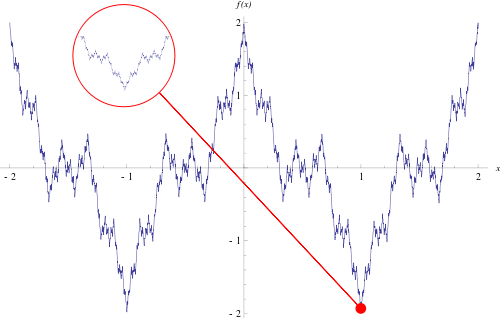
\includegraphics[width=0.8\textwidth]{media/weierstrass-pubdomain.png}
	\caption{The Weierstra\ss\ Function (image from \cite{img:weierstrass}).}
\end{figure}

Let's even put aside the pathology.
If I tell you the value of a real smooth function on the interval $[-1, 1]$,
that still doesn't tell you anything about the function as a whole.
It could be literally anything, because it's somehow possible to ``fuse together'' smooth functions.

So what about complex functions?
If you just consider them as functions $\RR^2 \to \RR^2$, you now have the interesting property
that you can integrate along things that are not just line segments: you can write integrals
across curves in the plane.
But $\CC$ has something more: it is a \emph{field}, so you can \emph{multiply} and \emph{divide} two complex numbers.

So we restrict our attention to differentiable functions called \emph{holomorphic functions}.
It turns out that the multiplication on $\CC$ makes all the difference.
The primary theme in what follows is that holomorphic functions are \emph{really, really nice},
and that knowing tiny amounts of data about the function can determine all its values.
%In particular, they are highly \emph{rigid} and \emph{regular}.

The two main highlights of this chapter,
from which all other results are more or less corollaries:
\begin{itemize}
	\ii Contour integrals of loops are always zero.
	\ii A holomorphic function is essentially given by its Taylor series;
	in particular, single-differentiable implies infinitely differentiable.
	Thus, holomorphic functions behave quite like polynomials.
\end{itemize}
Some of the resulting corollaries:
\begin{itemize}
	\ii It'll turn out that knowing just the values of a holomorphic function
	on the boundary of the unit circle will tell you the values in its interior.
	\ii Knowing just the values of the function at $1$, $\half$, $\frac13$, \dots
	are enough to determine the whole function!
	\ii Bounded holomorphic functions $\CC \to \CC$ must be constant
	\ii And more\dots
\end{itemize}

As \cite{ref:pugh} writes: ``Complex analysis is the good twin and real analysis is the evil one: beautiful formulas and elegant theorems seem to blossom spontaneously in the complex domain, while toil and pathology rule the reals''.


\section{Complex differentiation}
\prototype{Polynomials are holomorphic; $\ol z$ is not.}
Let $f : U \to \CC$ be a complex function.
Then for some $z_0 \in U$, we define the \vocab{derivative} at $z_0$ to be
\[
	\lim_{h \to 0} \frac{f(z_0+h) - f(z_0)}{h}.
\]
Note that this limit may not exist; when it does we say $f$ is \vocab{differentiable} at $z_0$.

What do I mean by a ``complex'' limit $h \to 0$?
It's what you might expect: for every $\eps > 0$ there should be a $\delta > 0$
such that 
\[ 0 < \left\lvert h \right\rvert < \delta
	\implies
	\left\lvert \frac{f(z_0+h)-f(z_0)}{h} - L \right\rvert < \eps. \]
If you like topology, you are encouraged to think of this in terms of neighborhoods in the complex plane.
(This is why we require $U$ to be open: it makes it possible to take $\delta$-neighborhoods in it.)

But note that having a complex derivative is actually much stronger
than a real function having a derivative.
In the real line, $h$ can only approach zero from below and above,
and for the limit to exist we need the ``left limit'' to equal the ``right limit''.
But the complex numbers form a \emph{plane}: $h$ can approach zero
from many directions, and we need all the limits to be equal.

\begin{example}
	[Important: conjugation is \emph{not} holomorphic]
	Let $f(z) = \ol z$ be complex conjugation, $f : \CC \to \CC$.
	This function, despite its simple nature, is not holomorphic!
	Indeed, at $z=0$ we have,
	\[ \frac{f(h)-f(0)}{h} = \frac{\ol h}{h}. \]
	This does not have a limit as $h \to 0$, because depending
	on ``which direction'' we approach zero from we have different values.
	\begin{center}
		\begin{asy}
			size(7cm);
			dot("$0$", origin, dir(225));
			void meow(string s, real theta, real eps = 45, pen p) {
				draw( (dir(theta) * 0.8) -- (dir(theta) * 0.2), p+1);
				draw( (dir(theta) * 0.8) -- (dir(theta) * 0.2), p, Arrow);
				label(s, dir(theta)*0.5, dir(eps), p);
			}
			meow("$1$", 0, 90, blue);
			meow("$1$", 180, 90, blue);
			meow("$i$", -45, 45, heavygreen);
			meow("$-1$", 90, 0, red);
			label("$f(z) = \overline z$", dir(135));
			label("$\dfrac{f(0+h)-f(0)}{h}$", dir(135)-0.35*dir(90));

			import graph;
			graph.xaxis("Re", -1, 1, grey, NoTicks, Arrows);
			graph.yaxis("Im", -1, 1, grey, NoTicks, Arrows);
		\end{asy}
	\end{center}
\end{example}

If a function $f : U \to \CC$ is complex differentiable
at all the points in its domain it is called \vocab{holomorphic}.
In the special case of a holomorphic function with domain $U = \CC$,
we call the function \vocab{entire}.\footnote{Sorry, I know the word ``holomorphic'' sounds so much cooler. I'll try to do things more generally for that sole reason.}

\begin{example}
	[Examples of holomorphic functions]
	In all the examples below, the derivative of the function
	is the same as in their real analogues
	(e.g.\ the derivative of $e^z$ is $e^z$).
	\begin{enumerate}[(a)]
		\ii Any polynomial $z \mapsto z^n + c_{n-1} z^{n-1} + \dots + c_0$ is holomorphic.
		\ii The complex exponential $\exp : x+yi \mapsto e^x (\cos y + i \sin y)$
		can be shown to be holomorphic.
		\ii $\sin$ and $\cos$ are holomorphic when extended
		to the complex plane by $\cos z = \frac{e^{iz}+e^{-iz}}{2}$
		and $\sin z = \frac{e^{iz}-e^{-iz}}{2}$.
		\ii As usual, the sum, product, chain rules and so on apply,
		and hence \textbf{sums, products, nonzero quotients,
		and compositions of holomorphic functions are also holomorphic}.
	\end{enumerate}
\end{example}
You are welcome to try and prove these results, but I won't bother to do so.

\section{Contour integrals}
\prototype{$\oint_\gamma z^m \; dz$ around the unit circle.}
In the real line we knew how to integrate a function across a line segment $[a,b]$:
essentially, we'd ``follow along'' the line segment adding up the values of $f$ we see
to get some area.
Unlike in the real line, in the complex plane we have the power to integrate
over arbitrary paths: for example, we might compute an integral around a unit circle.
A contour integral lets us formalize this.

First of all, if $f : \RR \to \CC$ and $f(t) = u(t) + iv(t)$ for $u,v \in \RR$,
we can define an integral $\int_a^b$ by just adding the real and imaginary parts:
\[ \int_a^b f(t) \; dt
	= \left( \int_a^b u(t) \; dt \right)
	+ i \left( \int_a^b v(t) \; dt \right). \]
Now let $\alpha : [a,b] \to \CC$ be a path, thought of as
a complex differentiable\footnote{This isn't entirely correct here:
	you want the path $\alpha$ to be continuous and mostly differentiable,
	but you allow a finite number of points to have ``sharp bends''; in other words,
	you can consider paths which are combinations of $n$ smooth pieces.
	But for this we also require that $\alpha$ has ``bounded length''.} function.
Such a path is called a \vocab{contour},
and we define its \vocab{contour integral} by
\[
	\oint_\alpha f(z) \; dz
	= \int_a^b f(\alpha(t)) \cdot \alpha'(t) \; dt.
\]
You can almost think of this as a $u$-substitution (which is where the $\alpha'$ comes from).
In particular, it turns out this integral does not depend on how $\alpha$ is ``parametrized'':
a circle given by \[ [0,2\pi] \to \CC : t \mapsto e^{it} \]
and another circle given by \[ [0,1] \to \CC : t \mapsto e^{2\pi i t} \]
and yet another circle given by \[ [0,1] \to \CC : t \mapsto e^{2 \pi i t^5} \]
will all give the same contour integral, because the paths they represent have the same
geometric description: ``run around the unit circle once''.

In what follows I try to use $\alpha$ for general contours and $\gamma$ in the special case of loops.

Let's see an example of a contour integral.
\begin{theorem}
	\label{thm:central_cauchy_computation}
	Take $\gamma : [0,2\pi] \to \CC$ to be the unit circle specified by 
	\[ t \mapsto e^{it}. \]
	Then for any integer $m$, we have
	\[ \oint_\gamma z^{m} \; dz
		=
		\begin{cases}
			2\pi i & m = -1 \\
			0 & \text{otherwise}
		\end{cases}
		\]
\end{theorem}
\begin{proof}
	The derivative of $e^{it}$ is $i e^{it}$.
	So, by definition the answer is the value of
	\begin{align*}
		\int_0^{2\pi} (e^{it})^m \cdot (ie^{it}) \; dt
		&= \int_0^{2\pi} i(e^{it})^{1+m} \; dt \\
		&= i \int_0^{2\pi} \cos [(1+m)t] + i \sin [(1+m)t] \; dt \\
		&= - \int_0^{2\pi} \sin [(1+m)t] \; dt + i \int_0^{2\pi} \cos [(1+m)t] \; dt.
	\end{align*}
	This is now an elementary calculus question.
	One can see that this equals $2\pi i$ if $m=-1$ and
	otherwise the integrals vanish.
\end{proof}
Let me try to explain why this intuitively ought to be true for $m=0$.
In that case we just have $\oint_\gamma 1 \; dz$.
So as the integral walks around the unit circle, it ``sums up'' all the tangent vectors
at every point (that's the direction it's walking in), multiplied by $1$.
And given the nice symmetry of the circle, it should come as no surprise that everything cancels out.
The theorem says that even if we multiply by $z^m$ for $m \neq -1$, we get the same cancellation.

\begin{center}
	\begin{asy}
		size(5cm);
		draw(unitcircle, dashed);
		void arrow(real theta) {
			pair P = dir(theta);
			dot(P);
			pair delta = 0.4*P*dir(90);
			draw( P--(P+delta), EndArrow );
		}
		arrow(0);
		arrow(50);
		arrow(140);
		arrow(210);
		arrow(300);
	\end{asy}
\end{center}

\begin{definition}
	Given $\alpha : [0,1] \to \CC$,
	we denote by $\ol\alpha$ the ``backwards'' contour
	$\ol\alpha(t) = \alpha(1-t)$.
\end{definition}

\begin{ques}
	What's the relation between $\oint_\alpha f \; dz$ and $\oint_{\ol\alpha} f \; dz$?
	Prove it.
\end{ques}

This might seem a little boring.
Things will get really cool really soon, I promise.

\section{Cauchy-Goursat theorem}
\prototype{$\oint_\gamma z^m \; dz = 0$ for $m \ge 0$. But if $m < 0$, Cauchy's theorem does not apply.}
Let $\Omega \subseteq \CC$ be simply connected (for example, $\Omega = \CC$),
and consider two paths $\alpha$, $\beta$ with the same start and end points.

\begin{center}
	\begin{asy}
		unitsize(0.8cm);
		bigbox("$\Omega$");
		pair A = Drawing((-3,0));
		pair B = Drawing((3,0));
		draw(A..(-2,0.5)..MP("\alpha", (0,2), dir(90))..(1,1.2)..B, red, EndArrow);
		draw(A----MP("\beta", (A+B)/2, dir(-90))--B, blue, EndArrow);
	\end{asy}
\end{center}

What's the relation between $\oint_\alpha f(z) \; dz$ and $\oint_\beta f(z) \; dz$?
You might expect there to be some relation between them, considering that the space $\Omega$ is simply connected.
But you probably wouldn't expect there to be \emph{much} of a relation.

As a concrete example, let $\Psi : \CC \to \CC$ be the function $z \mapsto z - \Re[z]$
(for example, $\Psi(2015+3i) = 3i$). Let's consider two paths from $-1$ to $1$.
Thus $\beta$ just walking along the real axis, and $\alpha$ which follows an upper semicircle.

\begin{center}
	\begin{asy}
		pair A = Drawing("-1", dir(180), dir(-90));
		pair B = Drawing("1", dir(0), dir(-90));
		draw(arc(origin, 1, 180, 0), red, EndArrow);
		MP("\alpha", dir(90), dir(90));
		draw(A--B, blue, EndArrow);
		MP("\beta", 0, dir(-90));
	\end{asy}
\end{center}

Obviously $\oint_\beta \Psi(z) \; dz = 0$.
But heaven knows what $\oint_\alpha \Psi(z) \; dz$ is supposed to equal.
We can compute it now just out of non-laziness.
If you like, you are welcome to compute it yourself (it's a little annoying but not hard).
If I myself didn't mess up, it is
\[ \oint_\alpha \Psi(z) \; dz = - \oint_{\ol\alpha} \Psi(z) \; dz
= - \int_0^\pi (i \sin(t)) \cdot ie^{it} \; dt = \half\pi i \]
which in particular is not zero.

But somehow $\Psi$ is not a really natural function.
It's not respecting any of the nice, continuous structure of $\CC$ since
it just rudely lops off the real part of its inputs.
More precisely,
\begin{ques}
	Show that $\Psi(z) = z - \Re[z]$ is not holomorphic.
	(Hint: $\ol z$ is not holomorphic.)
\end{ques}

Now here's a miracle: for holomorphic functions, the two integrals are \emph{always equal}.
Equivalently, (by considering $\alpha$ followed by $\ol\beta$) contour integrals of loops are always zero.
This is the celebrated Cauchy-Goursat theorem
(also called the Cauchy integral theorem,
but later we'll have a ``Cauchy Integral Formula'' so blah).

\begin{theorem}
	[Cauchy-Goursat theorem]
	Let $\gamma$ be a loop, and $f : \Omega \to \CC$ a holomorphic function
	where $\Omega$ is open in $\CC$ and simply connected.
	Then
	\[ \oint_\gamma f(z) \; dz = 0. \]
\end{theorem}
\begin{remark}[Sanity check]
	This might look surprising considering that we saw $\oint_\gamma z^{-1} \; dz = 2 \pi i$ earlier.
	The subtlety is that $z^{-1}$ is not even defined at $z = 0$.
	On the other hand, the function $\CC \setminus \{0\} \to \CC$ by $z \mapsto \frac 1z$ \emph{is} holomorphic!
	The defect now is that $\Omega = \CC \setminus \{0\}$ is not simply connected.
	So the theorem passes our sanity checks, albeit just barely.
\end{remark}

The typical proof of Cauchy's Theorem assumes additionally
that the partial derivatives of $f$ are continuous
and then applies the so-called Green's theorem.
But it was Goursat who successfully proved the fully general theorem we've stated above,
which assumed only that $f$ was holomorphic.
I'll only outline the proof, and very briefly.
You can show that if $f : \Omega \to \CC$ has an antiderivative $F : \Omega \to \CC$ which is also holomorphic,
and moreover $\Omega$ is simply connected, then you get a ``fundamental theorem of calculus'', a la
\[ \oint_\alpha f(z) \; dz = F(\alpha(b)) - F(\alpha(a)) \]
where $\alpha : [a,b] \to \CC$ is some path.
So to prove Cauchy-Goursat, you just have to show this antiderivative $F$ exists.
Goursat works very hard to prove the result in the special case that $\gamma$ is a triangle,
and hence by induction for any polygon.
Once he has the result for a rectangle, he uses this special case to construct the function $F$ explicitly.
Goursat then shows that $F$ is holomorphic, completing the proof.

Anyways, the theorem implies that $\oint_\gamma z^m \; dz = 0$ when $m \ge 0$.
So much for all our hard work earlier.
But so far we've only played with circles.
This theorem holds for \emph{any} contour which is a loop.
So what else can we do?

\section{Cauchy's integral theorem}
We now present a stunning application of Cauchy-Goursat, a ``representation theorem'':
essentially, it says that values of $f$ inside a disk
are determined by just the values on the boundary!
In fact, we even write down the exact formula.
As \cite{ref:dartmouth} says,
``any time a certain type of function satisfies some sort of representation theorem,
it is likely that many more deep theorems will follow.''
Let's pull back the curtain:

\begin{theorem}[Cauchy's integral formula]
	Let $\gamma : [0,2\pi] \to \CC$ be a circle in the plane given by $t \mapsto Re^{it}$,
	which bounds a disk $D$.
	Suppose $f : U \to \CC$ is holomorphic such that $U$ contains the circle and its interior.
	Then for any point $a$ in the interior of $D$, we have
	\[ 
		f(a)
		=
		\frac{1}{2\pi i} \oint_\gamma \frac{f(z)}{z-a} \; dz.
	\]
\end{theorem}
Note that we don't require $U$ to be simply connected, but the reason is pretty silly:
we're only going to ever integrate $f$ over $D$, which is an open disk, and hence the disk
is simply connected anyways.

The presence of $2\pi i$, which you saw earlier in the form $\oint_{\text{circle}} z^{-1} \; dz$,
is no accident.
In fact, that's the central result we're going to use to prove the result.

\begin{proof}
	There are several proofs out there, but I want to give the one that really
	draws out the power of Cauchy's theorem. Here's the picture we have:
	there's a point $a$ sitting inside a circle $\gamma$,
	and we want to get our hands on the value $f(a)$.
	\begin{center}
		\begin{asy}
			size(3cm);
			draw(unitcircle, dashed, MidArrow);
			MP("\gamma", dir(-45), dir(-45));
			pair a = 0.1 * dir(60);
			dot("$a$", a, dir(a));
		\end{asy}
	\end{center}
	We're going to do a trick: construct a \vocab{keyhole contour} $\Gamma_{\delta, \eps}$
	which has an outer circle $\gamma$, plus an inner circle $\ol{\gamma_\eps}$, which is a circle centered
	at $a$ with radius $\eps$, running clockwise (so that $\gamma_\eps$ runs counterclockwise).
	The ``width'' of the corridor is $\delta$. See picture:
	\begin{center}
		\begin{asy}
			size(4cm);
			MP("\gamma", dir(-45), dir(-45));
			pair a = 0.1 * dir(60);
			dot("$a$", a, dir(a));
			real delta_outer = 6;
			real delta_inner = 20;
			pair P = dir(60+delta_outer);
			pair Q = dir(60-delta_outer);
			draw(arc(origin, 1, 60+delta_outer, 360+60-delta_outer), MidArrow);
			draw(arc(a, 0.3, 60-delta_inner, -360+60+delta_inner), MidArrow);
			draw(dir(60-delta_outer)--(a+0.3*dir(60-delta_inner)), MidArrow);
			draw((a+0.3*dir(60+delta_inner))--dir(60+delta_outer), MidArrow);
			MP("\overline{\gamma_\varepsilon}", a+0.3*dir(225), dir(225));
		\end{asy}
	\end{center}
	Hence $\Gamma_{\delta,\eps}$ consists of four smooth curves.
	\begin{ques}
		Draw a \emph{simply connected} open set $\Omega$ which contains the entire
		$\Gamma_{\delta,\eps}$ but does not contain the point $a$.
	\end{ques}
	Hence, the function $\frac{f(z)}{z-a}$ manages to be holomorphic on all of $\Omega$.
	Thus Cauchy's theorem applies and tells us that
	\[
		0 = \oint_{\Gamma_{\delta,\eps}} \frac{f(z)}{z-a} \; dz.
	\]
	As we let $\delta \to 0$, the two walls of the keyhole will cancel each other (because $f$ is continuous,
	and the walls run in opposite directions).
	So taking the limit as $\delta \to 0$, we are left with just $\gamma$ and $\gamma_\eps$, 
	which (taking again orientation into account) gives
	\[
		\oint_{\gamma} \frac{f(z)}{z-a} \; dz
		= - \oint_{\ol{\gamma_\eps}} \frac{f(z)}{z-a} \; dz
		= \oint_{\gamma_\eps} \frac{f(z)}{z-a} \; dz.
	\]
	Thus \textbf{we've managed to replace $\gamma$ with a much smaller circle $\gamma_\eps$ centered around $a$},
	and the rest is just algebra.

	To compute the last quantity, write
	\begin{align*}
		\oint_{\gamma_\eps} \frac{f(z)}{z-a} \; dz
		&=
		\oint_{\gamma_\eps} \frac{f(z)-f(a)}{z-a} \; dz
		+
		f(a) \cdot \oint_{\gamma_\eps} \frac{1}{z-a} \; dz \\
		&=
		\oint_{\gamma_\eps} \frac{f(z)-f(a)}{z-a} \; dz
		+
		2\pi i f(a).
	\end{align*}
	where we've used \Cref{thm:central_cauchy_computation}
	Thus, all we have to do is show that 
	\[ \oint_{\gamma_\eps} \frac{f(z)-f(a)}{z-a} \; dz = 0. \]
	For this we can basically use the weakest bound possible, the so-called $ML$ lemma
	which I'll just cite without proof:
	it just says ``bound the function everywhere by its maximum''.
	\begin{lemma}
		[$ML$ estimation lemma]
		Let $f$ be a holomorphic function and $\alpha$ a path.
		Suppose $M = \max_{z \text{ on } \alpha} \left\lvert f(z) \right\rvert$, and
		let $L$ be the length of $\alpha$.
		Then
		\[ \left\lvert \oint_\alpha f(z) \; dz \right\rvert \le ML. \]
	\end{lemma}
	(This is straightforward to prove if you know the definition of length:
	$L = \int_a^b \alpha'(t) \; dt$, where $\alpha : [a,b] \to \CC$.)

	Anyways, as $\eps \to 0$, the quantity $\frac{f(z)-f(a)}{z-a}$ just approaches $f'(a)$,
	and so for small enough $\eps$ (i.e.\ $z$ close to $a$) there's some upper bound $M$.
	Yet the length of $\gamma_\eps$ is just the circumference $2\pi \eps$.
	So the $ML$ lemma says that
	\[ \left\lvert \oint_{\gamma_\eps} \frac{f(z)-f(a)}{z-a} \right\rvert
		\le 2\pi\eps \cdot M \to 0
	\]
	as desired.
\end{proof}

\section{Holomorphic functions are analytic}
\prototype{Imagine a formal series $\sum_k c_kx^k$!}
In the setup of the previous problem, we have a circle $\gamma : [0,2\pi] \to \CC$
and a holomorphic function $U \to \CC$ which contains the disk $D$.
We can write
\begin{align*}
	f(a) &= \frac{1}{2\pi i} \oint_\gamma \frac{f(z)}{z-a} \; dz \\
	&= \frac{1}{2\pi i} \oint_\gamma \frac{f(z)/z}{1 - \frac az} \; dz \\
	&= \frac{1}{2\pi i} \oint_\gamma f(z)/z \cdot \sum_{k \ge 0} \left( \frac az \right)^k \; dz \\
	\intertext{You can prove (using the so-called Weierstrass M-test) that the summation order can be switched:}
	&= \frac{1}{2\pi i} \sum_{k \ge 0} \oint_\gamma \frac{f(z)}{z} \cdot \left( \frac az \right)^k \; dz \\
	&= \frac{1}{2\pi i} \sum_{k \ge 0} \oint_\gamma a^k \cdot \frac{f(z)}{z^{k+1}} \; dz \\
	&=  \sum_{k \ge 0} \left( \frac{1}{2\pi i}\oint_\gamma \frac{f(z)}{z^{k+1}} \; dz \right) a^k \\
	\intertext{Letting $c_k =  \frac{1}{2\pi i}\oint_\gamma \frac{f(z)}{z^{k+1}} \; dz$, and noting
this is independent of $a$, this is}
	&=  \sum_{k \ge 0} c_k a^k
\end{align*}
and that's the miracle: holomorphic functions are given by a Taylor series!
This is one of the biggest results in complex analysis.
Moreover, we also know that \[ c_k = \frac{f^{(k)}(0)}{k!} \] from AP Calculus (if you don't see this,
just take the derivative $k$ times), and this gives us $f^{(k)}(0) = k! \cdot c_k$.

Naturally, we can do this with any circle (not just one centered at zero).
So let's state the full result below, with arbitrary center $p$.

\begin{theorem}
	[Cauchy's differentiation formula]
	Let $f : U \to \CC$ be a holomorphic function and let $D$ be a disk centered at point $p$
	bounded by a circle $\gamma$.  Suppose $D$ is contained inside $U$.
	Then $f$ is given everywhere in $D$ by a Taylor series
	\[ 
		f(z) = c_0 + c_1(z-p) + c_2(z-p)^2 + \dots
	\]
	where
	\[
		c_k = \frac{f^{k}(p)}{k!} = \frac{1}{2\pi i} \oint_\gamma \frac{f(w-p)}{(w-p)^{k+1}} \; dw
	\]
	In particular, 
	\[ f^{(k)}(p) = k! c_k = \frac{k!}{2\pi i} \oint_\gamma \frac{f(w-p)}{(w-p)^{k+1}} \; dw. \]
\end{theorem}

Most importantly,
\begin{moral}
	Over any disk,
	a holomorphic function is given
	exactly by a Taylor series.
\end{moral}
This establishes a result we stated at the beginning of the chapter:
that a function being complex differentiable once means it is not only infinitely differentiable,
but in fact equal to its Taylor series.

I should maybe emphasize a small subtlety of the result:
the Taylor series centered at $p$ is only valid in a disk centered at $p$ which lies entirely in the domain $U$.
If $U = \CC$ this is no issue, since you can make the disk big enough to accommodate any point you want.
It's more subtle in the case that $U$ is, for example, a square; you can't cover the entire square
with a disk centered at some point without going outside the square.
However, since $U$ is open we can at any rate at least find some neighborhood for which the Taylor
series is correct -- in stark contrast to the real case.
Indeed, as you'll see in the problems,
the existence of a Taylor series is incredibly powerful.

\section\problemhead
These aren't olympiad problems, but I think they're especially nice!
In the next complex analysis chapter we'll see some more nice applications.

The first few results are the most important.


\begin{sproblem}
	[Liouville's theorem]
	\gim
	Let $f : \CC \to \CC$ be an entire function.
	Suppose that $\left\lvert f(z) \right\rvert < 1000$ for all complex numbers $z$.
	Prove that $f$ is a constant function.
	\begin{hint}
		Look at the Taylor series of $f$,
		and use Cauchy's differentiation formula to
		show that each of the larger coefficients must be zero.
	\end{hint}
%	\footnote{%
%	It's true more generally that if
%	$\left\lvert f(z) \right\rvert < A+B\left\lvert z \right\rvert^n$
%	for some constants $A$ and $B$,
%	then $f$ is a polynomial of degree at most $n$.
%	The proof is just induction on $n$ with the case $n=0$ being the theorem.}
\end{sproblem}


\begin{sproblem}[Zeros are isolated]
	An \vocab{isolated set} in the complex plane is a set of points $S$ such that
	around each point in $S$, one can draw a neighborhood not intersecting any other point of $S$.

	Show that the zero set of any nonzero holomorphic function $f : U \to \CC$
	is an isolated set, unless there exists a neighborhood of $f$ which is identically zero.
	\begin{hint}
		Proceed by contradiction, meaning there exists a sequence $z_1, z_2, \dots \to z$
		where $0 = f(z_1) = f(z_2) = \dots$ all distinct.
		Prove that $f = 0$ on some small neighborhood and apply the identity theorem.
	\end{hint}
	\begin{sol}
		Proceed by contradiction, meaning there exists a sequence $z_1, z_2, \dots \to z$
		where $0 = f(z_1) = f(z_2) = \dots$ all distinct.
		WLOG set $z=0$.
		Look at the Taylor series of $f$ around $z=0$.
		Since it isn't uniformly zero by assumption, write it as $a_Nz^N + a_{N+1}z^{N+1} + \dots$, $a_N \neq 0$.
		But by continuity of $h(z) = a_N + a_{N+1}z + \dots$ there is some
		neighborhood of zero where $h(z) \neq 0$.
	\end{sol}
\end{sproblem}

\begin{sproblem}
	[Identity theorem]
	\gim
	Let $f, g : U \to \CC$ be holomorphic, and assume that $U$ is connected.
	Prove that if $f$ and $g$ agree on some small neighborhood, then $f = g$.
	\begin{hint}
		Take the interior of the agreeing points;
		show that this set is closed, which implies the conclusion.
	\end{hint}
	\begin{sol}
		Let $S$ be the interior of the points satisfying $f=g$.
		By definition $S$ is open.
		By the previous part, $S$ is closed: if $z_i \to z$ and $z_i \in S$,
		then $f=g$ in some neighborhood of $z$, hence $z \in S$.
		Since $S$ is clopen and nonempty, $S = U$.
	\end{sol}
\end{sproblem}

\begin{figure}[ht]
	\centering
	\snsd[height=6cm]{bounded-like-complex-sine.jpg}
	\caption{Complex functions are unbounded. (Source: \cite{img:snsd}.)}
\end{figure}


%\begin{dproblem}
%	[Mean Value Property]
%	Let $f : U \to \CC$ be holomorphic.
%	Assume that $z_0 \in U$ and the disk centered at $z_0$
%	with radius $r > 0$ is contained inside $U$. Show that
%	\[ f(z_0) = \frac{1}{2\pi} \int_0^{2\pi} f(z_0+re^{it}) \; dt. \]
%	In other words, $f(z_0)$ is the average of $f$ along the circle.
%	\begin{hint}
%		Evaluate $\oint_\gamma \frac{f(w)}{w-z_0} \; dw$ over the circle.
%	\end{hint}
%\end{dproblem}

\begin{dproblem}[Maximums Occur On Boundaries]
	Let $f : U \to \CC$ be holomorphic, let $Y \subseteq U$ be compact,
	and let $\partial Y$ be boundary\footnote{
		The boundary $\partial Y$ is the set of points $p$
		such that no open neighborhood of $p$ is contained in $Y$.
		It is also a compact set if $Y$ is compact.
	} of $Y$.
	Show that
	\[ \max_{z \in Y} \left\lvert f(z) \right\rvert
		= \max_{z \in \partial Y} \left\lvert f(z) \right\rvert. \]
	In other words, the maximum values of $\left\lvert f \right\rvert$ occur
	on the boundary. (Such maximums exist by compactness.)
\end{dproblem}

\begin{problem}
	[Harvard quals]
	Let $f : \CC \to \CC$ be a nonconstant entire function.
	Prove that $f``(\CC)$ is dense in $\CC$.
	(In fact, a much stronger result is true:
	Little Picard's theorem says that the image of a nonconstant
	entire function omits at most one point.)
	\begin{hint}
		Liouville. Look at $\frac{1}{f(z)-w}$.
	\end{hint}
	\begin{sol}
		Suppose we want to show that there's a point
		in the image within $\eps$ of a given a point $w \in \CC$.
		Look at $\frac{1}{f(z) - w}$ and use Liouville's theorem.
	\end{sol}
\end{problem}

%\begin{dproblem}
%	[Liouiville's theorem extended]
%	Let $f : \CC \to \CC$ be entire.
%	\begin{enumerate}[(a)]
%		\ii Show that if $\left\lvert f(z) \right\rvert < C \left\lvert z \right\rvert^{1000}$
%		for some constant $C$, then $f$ is a polynomial of degree at most $1000$.
%		\ii Show that the image $f``(\CC)$ is dense in $\CC$,
%		unless $f$ is constant.
%	\end{enumerate}
%	\begin{hint}
%		Part (a) is the same proof of the original Louiville's theorem.
%
%		For part (b), assume it's not dense and misses a circle at $w$
%		with radius $\eps$. Look at $\frac{1}{f(z)-w}$ and show it's bounded.
%	\end{hint}
%\end{dproblem}

%\begin{problem}
%	Show that a nonzero entire function can have at most countably many zeros,
%	and give an example where equality occurs.
%	\begin{hint}
%		Assume there are uncountably many zeros
%		and do a pigeonhole style argument to force them to
%		accumulate at some point.
%		Then apply the identity theorem.
%		Equality occurs at $\sin(z)$.
%	\end{hint}
%\end{problem}

\chapter{Meromorophic Functions}
\section{The Second Nicest Functions on Earth}
Last time we studied holomorphic functions, which I dubbed ``the nicest functions on Earth'',
and the incredibly nice properties they possessed, such as
\[
	\oint_\gamma f(z) \; dz = 0.
\]
We saw an example of a function that was ``almost holomorphic'', namely $\frac 1z$, which instead satisfied
\[
	\oint_{\gamma} \frac 1z \; dz
	= \frac{1}{2\pi i}
\]
for $\gamma(t) = e^{it}$ the unit circle.
But $\frac 1z$ was ``barely'' not holomorphic: it simply has a defect at the point $z=0$.
We now want to extend our results to such functions.

In this chapter we will study the so-called ``second nicest functions on Earth'',
the \emph{meromorphic functions}, or better yet, the ``almost holomorphic'' functions.
It turns out that, instead of just getting $\oint_\gamma f(z) \; dz = 0$ like we did in
the holomorphic case, the line integrals will actually be used to \emph{count the number of poles}
inside the loop $\gamma$. It's ridiculous, I know.

\section{Meromorphic Functions}
\prototype{$\frac 1z$, with a pole of order $1$ and residue $1$ at $z=0$.}

Let $U$ be an open subset of $\CC$ again.
We want to consider functions $f$ defined on all points in $U$
except for a set of ``isolated'' singularities;
for example, something like \[ \frac{1}{z(z+1)(z^2+1)} \] which is defined
for all $z$ other than $z=0$, $z=-1$ and $z=i$.
Or even \[ \frac{1}{\sin(2\pi z)}, \] which is defined at every $z$ which is \emph{not} an integer.
Even though there's infinitely many points, they are not really that close together.

Let's make these notions precise.
First, let's make the notion of this ``division by zero'' precise.
\begin{definition}
	Let $p \in \CC$ be any point.
	By a \vocab{deleted neighborhood} of $p$ we mean an open set of the form $U - \{p\}$,
	where $U$ is a neighborhood of $p$.
\end{definition}
\begin{example}
	For example, a deleted neighborhood of $0$ might be the set
	\[ \left\{ z \in \CC \mid 0 < \left\lvert z \right\rvert < \frac{1}{1000} \right\}. \]
	It quite literally looks like an open disk with a hole poked into it.
\end{example}

\begin{definition}
	Let $U$ be an open set and $p$ a point inside it.
	A function $f : U \to \CC$ is said to have a \vocab{pole} at $p$
	if for some deleted neighborhood of $p$ it admits a \vocab{Laurent series}
	\[
		f(z) =
		\frac{c_{-m}}{(z-p)^m}
		+ \frac{c_{-m+1}}{(z-p)^{m-1}}
		+ \dots
		+ \frac{c_{-1}}{z-p} + c_0 + c_1 (z-p) + \dots
	\]
	for some positive integer $m$ (with $c_{-m} \neq 0$),
\end{definition}

Note that the trailing end \emph{must} terminate.
If we cannot do so, we say that $p$ is an \vocab{essential singularity} instead.\footnote{%
	On the other hand, if $m \ge 0$ we just say $p$ is a \vocab{removable singularity}
	because you could just define $f(z)$ and ``patch'' the hole.}

\begin{abuse}
	We'll often say something like ``consider the function $f : \CC \to \CC$ by $z \mapsto \frac 1z$''.
	Of course this isn't completely correct, because $f$ doesn't have a value at $z=0$.
	If I was going to be completely rigorous I would just set $f(0) = 2015$ or something and move on
	with life, but for all intents let's just think of it as ``undefined at $z=0$''.

	Why don't I just write $g : \CC \setminus \{0\} \to \CC$?
	The reason I have to do this is that it's still important 
	for $f$ to remember it's ``trying'' to be holomorphic on $\CC$,
	even if isn't assigned a value at $z=0$.
	As a function $\CC \setminus \{0\} \to \CC$ the function $\frac 1z$ is actually holomorphic.
\end{abuse}

\begin{definition}
	Bear with me for a moment here: the integer $m$ called the \vocab{order} of the pole.
	For reasons that will be clear later (bear with me for now), we also
	give the coefficient $c_{-1}$ a name, the \vocab{residue} of $f$ at $p$,
	which we write $\Res(f;p)$.
\end{definition}

Although I haven't told you yet what a meromorphic function is,
here are examples nonetheless.
\begin{example}
	[Examples of Meromorphic Functions]
	\listhack
	\begin{enumerate}[(a)]
		\ii Any holomorphic function is a meromorphic function which happens to have no poles.
		Stupid, yes.
		\ii The function $\CC \to \CC$ by $z \mapsto 100z\inv$ for $z \neq 0$
		but undefined at zero is a meromorphic function.
		Its only pole is at zero, which has order $1$ and residue $100$.
		\ii The function $\CC \to \CC$ by $z \mapsto z^{-2015}$ is also a meromorphic function.
		Its only pole is at zero, and it has order $3$, and residue $0$.
		\ii The function $\CC \to \CC$ by $z \mapsto \frac{e^z}{z^2}$ is meromorphic,
		with the Laurent series at $z=0$ given by
		\[
			\frac{e^z}{z^2}
			= \frac{1}{z^2} + \frac{1}{z} + \frac{1}{2} + \frac{z}{6} + \frac{z^2}{24} + \frac{z^3}{120}
			+ \dots.
		\]
		Hence the pole $z=0$ has order $2$ and residue $1$.
	\end{enumerate}
\end{example}
\begin{example}
	[A Rational Meromorphic Functions]
	Consider the function $\CC \to \CC$ given  by
	\begin{align*}
		z &\mapsto \frac{z^4+1}{z(z-1)} \\
		&= z^2 + 1 + \frac 2z \cdot \frac{1}{z-1} \\
		&= z^2 + 1 + \frac 2z \left( 1 + z + z^2 + \dots  \right) \\
		&= \frac 2z + 3 + 2z + 3z^2 + 2z^3 + 2z^4 + 2z^5 + \dots 
	\end{align*}
	has a pole of order $1$ and residue $2$ at $z=0$.
	(It also has a pole of order $1$ at $z=1$; you are invited to compute the residue.)
\end{example}
\begin{example}
	[Function with Infinitely Many Poles]
	The function $\CC \to \CC$ by \[ z \mapsto \frac{1}{\sin(z)} \]
	has infinitely many poles: the numbers $z = 2\pi k$, where $k$ is an integer.
	Let's compute the Laurent series at just $z=0$:
	\begin{align*}
		\frac{1}{\sin(2\pi z)}
		&= \frac{1}{\frac{z}{1!} - \frac{z^3}{3!} + \frac{z^5}{5!} - \dots} \\
		&= \frac{1/z}{\frac{1}{1!} - \frac{z^2}{3!} + \frac{z^4}{5!} - \dots} \\
		&= \frac 1z \cdot \frac{1}{1 - \left( \frac{z^2}{3!} - \frac{z^4}{5!} + \dots \right)} \\
		&= \frac 1z \sum_{k \ge 0} \left( \frac{z^2}{3!} - \frac{z^4}{5!} + \dots \right)^k.
	\end{align*}
	which is a Laurent series, though I have no clue what the coefficients are.
	You can at least see the residue; the constant term of that huge sum is $1$,
	so the residue is $1$.
	Also, the pole has order $1$.
\end{example}

The Laurent series, if it exists, is unique (as you might have guessed),
and by our result on holomorphic function it is actually valid for \emph{any}
disk centered at $p$ (minus the point $p$).
The part $\frac{c_{-1}}{z-p} + \dots + \frac{c_{-m}}{(z-p)^m}$ is called the \vocab{principal part},
and the rest of the series $c_0 + c_1(z-p) + \dots$ is called the \vocab{analytic part}.

Now that I have the examples written down I'll actually define a meromorphic function.
\begin{definition}
	Let $U$ be an open set, $S \subseteq U$.
	A function $f : U \to \CC$ is \vocab{meromorphic}
	if it is holomorphic when viewed as a function $U \setminus S \to \CC$,
	and moreover each $p \in S$ is a pole.
\end{definition}
We don't require $S$ to be finite (for example, $\frac{1}{\sin(2\pi z)}$ is meromorphic
and has poles whenever $z$ is an integer).
However, $S$ cannot be very big either.
To be precise, recall that for $p \in S$ to be a pole, $f$ must be defined on some
deleted neighborhood of $p$ -- thus that deleted neighborhood can't contain points of $S$.
So $S$ must be \emph{isolated}\footnote{This is an actual topological definition: a subset
of a topological space is called isolated if this condition holds}
in the sense that we can draw a neighborhood around
each point in $S$, so that no two neighborhoods intersect.


\begin{example}
	[Isolated Sets]
	\listhack
	\begin{enumerate}[(a)]
		\ii The set $\ZZ$, regarded as a subset of $\CC$, is a nice example of an isolated set
		which isn't finite: we can just take a $\frac{1}{2015}$-neighborhood around each point.
		\ii Even the set $\{\frac 1n \mid n \in 1,2,\dots \}$ is an isolated set.
		Take a disk of radius $0.001n^{-2015}$ around each point.
		
		However, no meromorphic function can actually have this set as its set of poles, since
		if a function (like $1/\sin(2\pi/z)$) had such poles it would also have to have a pole at $z=0$.
		Once we add in the point $0$, the set above is no longer an isolated set.

		In general, the set of poles must be closed.
		\ii The unit circle $S^1$, on the other hand, is not at all isolated.
	\end{enumerate}
\end{example}


Anyways, you may have noticed that most examples of meromorphic functions we gave
were of the form $A(z) / B(z)$ for holomorphic functions $A$ and $B$.
For example, \[ \frac 1z, \quad \frac{e^z}{z}, \quad \frac{1}{\sin z}, \] and so on.
In fact, this is true in general.
\begin{theorem}
	A function $f : U \to \CC$ is meromorphic
	if and only if it is the quotient $g/h$ of two holomorphic functions $g,h : U \to \CC$
	where $h$ is a nonzero function with zeros at each pole of $f$.
\end{theorem}
We won't prove this here, but the point is to take a function $h$ whose zeros exactly
correspond, with multiplicity, to the poles of $f$, so that $f \cdot h$ becomes holomorphic.
The tricky part is showing that such a function $h$ exists.

\section{Winding Numbers and the Residue Theorem}
Recall that for a counterclockwise circle $\gamma$ and a point $p$ inside it, we had
\[
	\oint_{\gamma} (z-p)^m \; dz =
	\begin{cases}
		0 & m \neq -1 \\
		2\pi i & m = -1
	\end{cases}
\]
where $m$ is an integer.
One can extend this result to in fact show that $\oint_\gamma (z-p)^m \; dz = 0$
for \emph{any} loop $\gamma$, where $m \neq -1$.
So we associate a special name for the nonzero value at $m=-1$.
\begin{definition}
	For a point $p \in \CC$ and a loop $\gamma$ not passing through it,
	we define the \vocab{winding number}, denoted $\Wind(p, \gamma)$, by
	\[
		\Wind(\gamma, p) = \frac{1}{2\pi i} \oint_{\gamma} \frac{1}{z-p} \; dz
	\]
\end{definition}
For example, our previous results we see that if $\gamma$ is a circle, we have
\[
	\Wind(\text{circle}, p)
	=
	\begin{cases}
		1 & \text{$p$ inside the circle} \\
		0 & \text{$p$ outside the circle}.
	\end{cases}
\]
If you've read the chapter of fundamental groups, then this is just the fundamental group
associated to $\CC \setminus \{p\}$.
In particular, the winding number is always an integer (the proof of this requires the complex logarithm,
so we omit it here).
In the simplest case the winding numbers are either $0$ or $1$.
\begin{definition}
	We say a loop $\gamma$ is \vocab{regular} if $\Wind(p, \gamma) = 1$
	for all points $p$ in the interior of $\gamma$ (for example,
	if $\gamma$ is a counterclockwise circle).
\end{definition}

With all these ingredients we get the following stunning generalization of the Cauchy-Goursat Theorem.
\begin{theorem}
	[Cauchy's Residue Theorem]
	Let $f : \Omega \to \CC$ be meromorphic, where $\Omega$ is simply connected.
	Then for any loop $\gamma$ not passing through any of its poles, we have
	\[
		\frac{1}{2\pi i} \oint_{\gamma} f(z) \; dz
		= \sum_{\text{pole $p$}} \Wind(\gamma, p) \Res(f; p).
	\]
	In particular, if $\gamma$ is regular then the countour integral is the sum of all the residues, in the form
	\[
		\frac{1}{2\pi i} \oint_{\gamma} f(z) \; dz
		= \sum_{\substack{\text{pole $p$} \\ \text{inside $\gamma$}}}  \Res(f; p).
	\]
\end{theorem}
\begin{ques}
	Verify that this result coincides
	with what you expect when you integrate $\oint_\gamma cz\inv \; dz$
	for $\gamma$ a counter-clockwise circle.
\end{ques}

The proof from here is not really too impressive -- the ``work'' was already
done in our statements about the winding number.
\begin{proof}
	Let the poles with nonzero winding number be $p_1, \dots, p_k$ (the others do not affect the sum).\footnote{
		To show that there must be finitely many such poles: recall that all our contours $\gamma : [a,b] \to \CC$
		are in fact bounded, so there is some big closed disk $D$ which contains all of $\gamma$.
		The poles outside $D$ thus have winding number zero.
		Now we cannot have infinitely many poles inside the disk $D$, for $D$ is compact and the
		set of poles is a closed and isolated set!}
	Then we can write $f$ in the form
	\[
		f(z) = g(z) + \sum_{i=1}^k P_i\left( \frac{1}{z-p_i} \right)
	\]
	where $P_i\left( \frac{1}{1-p_i} \right)$ is the principal part of the pole $p_i$.
	(For example, if $f(z) = \frac{z^3-z+1}{z(z+1)}$ we would write $f(z) = (z-1) + \frac1z - \frac1{1+z}$.)

	The point of doing so is that the function $g$ is homomorphic (we've removed all the ``bad'' parts), so 
	\[ \oint_{\gamma} g(z) \; dz = 0 \]
	by Cauchy-Goursat.

	On the other hand, if $P_i(x) = c_1x + c_2x^2 + \dots + c_d x^d$ then
	\begin{align*}
		\oint_{\gamma} P_i\left( \frac{1}{z-p_i} \right) \; dz
		&=
		\oint_{\gamma} c_1 \cdot \left( \frac{1}{z-p_i} \right) \; dz
		+ \oint_{\gamma} c_2 \cdot \left( \frac{1}{z-p_i} \right)^2 \; dz
		+ \dots \\
		&= c_1 \cdot \Wind(\gamma, p_i) + 0 + 0 + \dots \\
		&= \Wind(\gamma, p_i) \Res(f; p_i).
	\end{align*}
	which gives the conclusion.
\end{proof}

\section{Argument Principle}
One tricky application is as follows.
Given a polynomial $P(x) = (x-a_1)^{e_1}(x-a_2)^{e_2}\dots(x-a_n)^{e_n}$, you might know that we have
\[ \frac{P'(x)}{P(x)} = \frac{e_1}{x-a_1} + \frac{e_2}{x-a_2} + \dots + \frac{e_n}{x-a_n}. \]
The quantity $P'/P$ is called the \vocab{logarithmic derivative}, as it is the derivative of $\log P$.
This trick allows us to convert zeros of $P$ into poles of $P'/P$ with order $1$;
moreover the residues of these poles are the multiplicities of the roots.

In an analogous fashion, we can obtain a similar result for any meromorphic function $f$.
\begin{proposition}
	[The Logarithmic Derivative]
	Let $f : U \to \CC$ be a meromorphic function.
	Then the logarithmic derivative $f'/f$ is meromorphic as a function from $U$ to $\CC$;
	its zeros and poles are:
	\begin{enumerate}[(i)]
		\ii A pole at each zero of $f$ whose residue is the multiplicity, and
		\ii A pole at each pole of $f$ whose residue is the negative of the pole's order.
	\end{enumerate}
\end{proposition}
In some sense you can almost think of a pole as a zero of negative multiplicity.
This spirit is exemplified below.
\begin{proof}
	Direct computation: for any zero/pole $a$ of $f$, let $f = (z-a)^k g(z)$ (where $g(a) \neq 0$).
	Here $k$ is the multiplicity for $a$ a zero and the negative of the order for $a$ a pole.
	Now $f' = (z-a)^k g'(z) + k(z-a)^{k-1} g(z)$, so
	\[ \frac{f'}{f} = \frac{g'(z)}{g(z)} + \frac{k}{z-a}. \qedhere \]
\end{proof}

Using this trick you can determine the number of zeros and poles inside a regular closed curve,
using the so-called Argument Principle.

\begin{theorem}
	[Argument Principle]
	Let $\gamma$ be a regular curve.
	Suppose $f : U \to \CC$ is meromorphic inside and on $\gamma$, and
	none of its zeros ore poles lie on $\gamma$.
	Then
	\[
		\frac{1}{2\pi i} \oint_\gamma \frac{f'}{f} \; dz
		= Z - P
	\]
	where $Z$ is the number of zeros inside $\gamma$ (counted with multiplicity)
	and $P$ is the number of poles inside $\gamma$ (again with multiplicity).
\end{theorem}
\begin{proof}
	Immediate by applying Cauchy's Residue Theorem alongside the preceding proposition.
	In fact you can generalizes to any curve $\gamma$ via the winding number:
	the integral is
	\[ \frac{1}{2\pi i} \oint_\gamma \frac{f'}{f} \; dz
		= \sum_{\text{zero $z$}} \Wind(\gamma,z)
		- \sum_{\text{pole $p$}} \Wind(\gamma,p) \]
	where the sums are with multiplicity.
\end{proof}

Thus the Argument Principle allows one to count zeros and poles inside any region of choice.

\begin{figure}[ht]
	\centering
	\includegraphics[height=6cm]{/home/evan/Pictures/TopologicalGG/pole-contour-residue.jpg}
	\caption{Throwing a contour around a pole lets us extract its residue.}
\end{figure}

Computers can use this to get information on functions whose values can be computed but whose behavior as a whole
is hard to understand.
Suppose you have a holomorphic function $f$, and you want to understand where its zeros are.
Then just start picking various circles $\gamma$.
Even with machine rounding error, the integral will be close enough to the true integer value that
we can decide how many zeros are in any given circle.
Numerical evidence for the Riemann Hypothesis (concerning the zeros of the Riemann zeta function)
can be obtained in this way.

\section{Philosophy: Why are holomorphic functions so nice?}
All the fun we've had with holomorphic and meromorphic functions comes down to the fact that
complex differentiability is such a strong requirement.
It's a small miracle that $\CC$, which \emph{a priori} looks only like $\RR^2$,
is in fact a field.
Moreover, $\RR^2$ has the nice property that one can draw nontrivial loops
(it's also true for real functions that $\int_a^a f \; dx = 0$, but this is not so interesting!),
and this makes the theory much more interesting.

As another piece of intuition from Siu\footnote{Harvard professor}:
If you try to get (left) differentiable functions over \emph{quaternions},
you find yourself with just linear functions.


\section\problemhead
% Looman-Menchoff Theorem?

\begin{problem}
	[Fundamental Theorem of Algebra]
	Prove that if $f$ is a nonzero polynomial of degree $n$
	then it has $n$ roots.
\end{problem}

\begin{dproblem}
	[Rouch\'e's Theorem]
	Let $f, g : U \to \CC$ be holomorphic functions, where $U$ contains the unit disk.
	Suppose that $\left\lvert f(z) \right\rvert > \left\lvert g(z) \right\rvert$
	for all $z$ on the unit circle.
	Prove that $f$ and $f+g$ have the same number of zeros
	which lie strictly inside the unit circle (counting multiplicities).
\end{dproblem}
	
\begin{problem}
	\yod
	Prove that the integral
	\[
		\int_{-\infty}^{\infty} \frac{\cos x}{x^2+1} \; dx
	\]
	converges and determine its value.
	\begin{hint}
		It's $\lim_{a \to \infty} \int_{-a}^{a} \frac{\cos x}{x^2+1} \; dx$.
		For each $a$, construct a semicircle.
	\end{hint}
	% semicircle integral

	% \quad \text{ and } \quad
	% \int_{-\infty}^{\infty} \frac{\sin x}{x^2+1} \; dx
\end{problem}

\begin{sproblem}
	Let $f : U \to \CC$ be a nonconstant holomorphic function.
	\begin{enumerate}[(a)]
		\ii (Open Mapping Theorem)
		Prove that the image of $f$ is open in $\CC$.\footnote{%
			Thus the image of \emph{any}
			open set $V \subseteq U$ is open in $\CC$
			(by repeating the proof for the restriction $f : V \to \CC$).
		}
		\ii (Maximum Modulus Principle)
		Show\footnote{One can also deduce the Maximum Modulus Principle
		from the Mean Value Property.} that $\left\lvert f \right\rvert$
		cannot have a maximum over $U$.
		That is, show that for any $z \in U$, there is some $z' \in U$
		such that $\left\lvert f(z) \right\rvert < \left\lvert f(z') \right\rvert$.
	\end{enumerate}
	% http://en.wikipedia.org/wiki/Open_mapping_theorem_(complex_analysis)
\end{sproblem}

\chapter{Holomorphic square roots and logarithms}
\label{ch:complex_log}
In this chapter we'll make sense of a holomorphic square root and logarithm.
The main results are \Cref{thm:nth_root}, \Cref{thm:holomorphic_log},
\Cref{cor:nonvanishing}, and \Cref{cor:principal}.
If you like, you can read just these four results, and skip the discussion of how they came to be.

Let $f : U \to \CC$ be a holomorphic function.
A \vocab{holomorphic $n$th root} of $f$ is a function $g : U \to \CC$
such that $f(z) = g(z)^n$ for all $z \in U$.
A \vocab{logarithm} of $f$ is a function $g : U \to \CC$
such that $f(z) = e^{g(z)}$ for all $z \in U$.
The main question we'll try to figure out is: when do these exist?
In particular, what if $f = \id$?

\section{Motivation: square root of a complex number}
To start us off, can we define $\sqrt z$ for any complex number $z$?

The first obvious problem that comes up is that for any $z$, there are
\emph{two} numbers $w$ such that $w^2 = z$.
How can we pick one to use?
For our ordinary square root function, we had a notion of ``positive'',
and so we simply took the positive root.

Let's expand on this: given
$ z = r \left( \cos\theta + i \sin\theta \right) $
(here $r \ge 0$) we should take the root to be
\[ w = \sqrt{r} \left( \cos \alpha + i \sin \alpha \right). \]
such that $2\alpha \equiv \theta \pmod{2\pi}$;
there are two choices for $\alpha \pmod{2\pi}$, differing by $\pi$.

For complex numbers, we don't have an obvious way to pick $\alpha$.
Nonetheless, perhaps we can also get away with an arbitrary distinction:
let's see what happens if we just choose the $\alpha$ with $-\half\pi < \alpha \le \half\pi$.

Pictured below are some points (in red)
and their images (in blue) under this ``upper-half'' square root.
The condition on $\alpha$ means we are forcing the blue points to lie on the right-half plane.

\begin{center}
	%% First Diagram
	\begin{asy}
		size(7cm);
		cplane();
		draw(origin--(4.2*dir(180)), grey+1.5);
		pair O = (-2.4, 1.1);
		pair T;
		pair[] A = new pair[8];
		real r = 1.44;
		real[] dirs = {45,45,45,135,175,255,-90,-75};
		for (int i=0; i<8; ++i) {
			A[i] = O + r*dir(i*45);
			dot("$z_{" + (string) i + "}$", A[i], dir(dirs[i]), red);
		}
		draw(A[0]..A[1]..A[2]..A[3]..A[4]..A[5]..A[6]..A[7]..cycle, red);

		real[] dirs = {-45, -15, 15, 45, 75, 150, 210, 230};
		for (int i=0; i<8; ++i) {
			A[i] = sqrt(abs(A[i]))*dir(degrees(A[i])/2);
			if (degrees(A[i]) > 90) { A[i] *= -1; }
			dot("$w_{" + (string) i + "}$", A[i], dir(dirs[i]), blue);
		}
		draw(A[7]..A[0]..A[1]..A[2]..A[3]..A[4]..A[5], blue);
	\end{asy}
\end{center}


Here, $w_i^2 = z_i$ for each $i$, and we are constraining the $w_i$
to lie in the right half of the complex plane.
We see there is an obvious issue: there is a big discontinuity near
the points $w_5$ and $w_7$!
The nearby point $w_6$ has been mapped very far away.
This discontinuity occurs since the points on the negative real axis are
at the ``boundary''.
For example, given $-4$, we send it to $-2i$, but we have hit the boundary:
in our interval $-\half\pi \le \alpha < \half\pi$, we are at the very left edge.


The negative real axis that we must not touch is
is what we will later call a \emph{branch cut},
but for now I call it a \textbf{ray of death}.
It is a warning to the red points: if you cross this line, you will die!
However, if we move the red circle just a little upwards
(so that it misses the negative real axis) this issue is avoided entirely,
and we get what seems to be a ``nice'' square root.

\begin{center}
	%% Second Diagram
	\begin{asy}
		size(7cm);
		cplane();
		draw(origin--(4.2*dir(180)), grey+1.5);
		pair O = (-2.8, 1.9);
		pair T;
		pair[] A = new pair[8];
		real r = 1.44;
		real[] dirs = {45,45,45,135,175,225,-45,-45};
		for (int i=0; i<8; ++i) {
			A[i] = O + r*dir(i*45);
			dot("$z_{" + (string) i + "}$", A[i], dir(dirs[i]), red);
		}
		draw(A[0]..A[1]..A[2]..A[3]..A[4]..A[5]..A[6]..A[7]..cycle, red);

		real[] dirs = {-45, -15, 15, 75, 105, 150, 210, 260};
		for (int i=0; i<8; ++i) {
			A[i] = sqrt(abs(A[i]))*dir(degrees(A[i])/2);
			if (degrees(A[i]) > 90) { A[i] *= -1; }
			dot("$w_{" + (string) i + "}$", A[i], dir(dirs[i]), blue);
		}
		draw(A[0]..A[1]..A[2]..A[3]..A[4]..A[5]..A[6]..A[7]..cycle, blue);
	\end{asy}
\end{center}

In fact, the ray of death is fairly arbitrary:
it is the set of ``boundary issues''
that arose when we picked $-\half\pi < \alpha \le \half\pi$.
Suppose we instead insisted on the interval $0 \le \alpha < \pi$;
then the ray of death would be the \emph{positive} real axis instead.
The earlier circle we had now works just fine.

\begin{center}
	%% Third Diagram
	\begin{asy}
		size(7cm);
		cplane();
		draw(origin--(4.2*dir(0)), grey+1.5);
		pair O = (-2.4, 1.1);
		pair T;
		pair[] A = new pair[8];
		real r = 1.44;
		real[] dirs = {-5,45,45,135,175,255,-90,-75};
		for (int i=0; i<8; ++i) {
			A[i] = O + r*dir(i*45);
			dot("$z_{" + (string) i + "}$", A[i], dir(dirs[i]), red);
		}
		draw(A[0]..A[1]..A[2]..A[3]..A[4]..A[5]..A[6]..A[7]..cycle, red);

		real[] dirs = {-45, -15, 15, 45, 75, 150, 180, 230};
		for (int i=0; i<8; ++i) {
			A[i] = sqrt(abs(A[i]))*dir(degrees(A[i])/2);
			dot("$w_{" + (string) i + "}$", A[i], dir(dirs[i]), blue);
		}
		draw(A[0]..A[1]..A[2]..A[3]..A[4]..A[5]..A[6]..A[7]..cycle, blue);
	\end{asy}
\end{center}

What we see is that picking a particular $\alpha$-interval
leads to a different set of edge cases, and hence a different ray of death.
The only thing these rays have in common is their starting point of zero.
In other words, given a red circle and a restriction of $\alpha$,
I can make a nice ``square rooted'' blue circle as long as the
ray of death misses it.

So, what exactly is going on?

\section{Square roots of holomorphic functions}
To get a picture of what's happening, we would like to consider a more
general problem: let $f: U \to \CC$ be holomorphic.
Then we want to decide whether there is a $g : U \to \CC$
such that \[ f(z) = g(z)^2. \]
Our previous discussion with $f = \id$
tells us we cannot hope to achieve this for $U = \CC$;
there is a ``half-ray'' which causes problems.
However, there are certainly functions $f : \CC \to \CC$ such that a $g$ exists.
As a simplest example, $f(z) = z^2$ should definitely have a square root!

Now let's see if we can fudge together a square root.
Earlier, what we did was try to specify a rule to force one of the two choices at each point.
This is unnecessarily strict.
Perhaps we can do something like the following:
start at a point in $z_0 \in U$, pick a square root $w_0$ of $f(z_0)$,
and then try to ``fudge'' from there the square roots of the other points.
What do I mean by fudge?
Well, suppose $z_1$ is a point very close to $z_0$,
and we want to pick a square root $w_1$ of $f(z_1)$.
While there are two choices, we also would expect $w_0$ to be close to $w_1$.
Unless we are highly unlucky, this should tell us which choice of $w_1$ to pick.
(Stupid concrete example: if I have taken the square root $-4.12i$ of $-17$
and then ask you to continue this square root to $-16$,
which sign should you pick for $\pm 4i$?)

There are two possible ways we could get unlucky in the scheme above:
first, if $w_0 = 0$, then we're sunk.
But even if we avoid that, we have to worry that
if we run a full loop in the complex plane,
we might end up in a different place from where we started.
For concreteness, consider the following situation, again with $f = \id$:

\begin{center}
	%% Fourth Diagram
	\begin{asy}
		size(7cm);
		cplane();
		pair O = origin;
		pair T;
		pair[] A = new pair[8];
		real r = 3.24;
		real[] dirs = {45,45,45,135,135,255,-45,-45};
		for (int i=0; i<8; ++i) {
			A[i] = O + r*dir(i*45);
			dot("$z_{" + (string) i + "}$", A[i], dir(dirs[i]), red);
		}
		draw(A[0]..A[1]..A[2]..A[3]..A[4]..A[5]..A[6]..A[7]..cycle, red);

		real[] dirs = {-65, -15, 15, 45, 45, 135, 143, 135};
		for (int i=0; i<8; ++i) {
			A[i] = sqrt(abs(A[i]))*dir(degrees(A[i])/2);
			dot("$w_{" + (string) i + "}$", A[i], dir(dirs[i]), blue);
		}
		draw(A[0]..A[1]..A[2]..A[3]..A[4]..A[5]..A[6]..A[7]..(-A[0]), blue);
	\end{asy}
\end{center}

We started at the point $z_0$, with one of its square roots as $w_0$.
We then wound a full red circle around the origin, only to find that at the end of it,
the blue arc is at a different place where it started!

The interval construction from earlier doesn't work either:
no matter how we pick the interval for $\alpha$,
any ray of death must hit our red circle.
The problem somehow lies with the fact that we have enclosed the 
very special point $0$.

Nevertheless, we know that if we take $f(z) = z^2$, then we don't run into any problems
with our ``make it up as you go'' procedure.
So, what exactly is going on?

\section{Covering projections}
By now, if you have read the part on algebraic topology,
this should all seem quite familiar.
The ``fudging'' procedure exactly describes the idea of a lifting.

More precisely, recall that there is a covering projection
\[ (-)^2 : \CC \setminus \{0\}
	\to \CC \setminus \{0\}. \]
Let $V = \left\{ z \in U \mid f(z) \neq 0 \right\}$.
For $z \in U \setminus V$, we already have the square root $g(z) = \sqrt{f(z)} = \sqrt 0 = 0$.
So the burden is completing $g : V \to \CC$.

Then essentially, what we are trying to do is construct a lifting $g$ for the following diagram:
\begin{diagram}
	&&& E = \CC \setminus \{0\} \\
	&& \ruTo(3,2)^{g} & \dTo_{p = (-)^2} \\
	V & \rTo_f && B = \CC \setminus \{0\}
\end{diagram}

Our map $p$ can be described as ``winding around twice''.
Our \Cref{thm:lifting} now tells us that this lifting exists if and only if
\[ f_\ast``(\pi_1(V)) \subseteq p_\ast``(\pi_1(E)) \]
is a subset of the image of $\pi_1(E)$ by $p$.
Since $B$ and $E$ are both punctured planes, we can identify them with $S^1$.
\begin{ques}
	Show that the image under $p$ is
	exactly $2\ZZ$ once we identify $\pi_1(B) = \ZZ$.
\end{ques}

That means that for any loop $\gamma$ in $V$, we need $f \circ \gamma$ to have an
\emph{even} winding number around $0 \in B$.
This amounts to
\[
	\frac{1}{2\pi} \oint_\gamma \frac{f'}{f} \; dz \in 2\ZZ
\]
since $f$ has no poles.

Replacing $2$ with $n$ and carrying over the discussion gives the first main result.
\begin{theorem}
	[Existence of holomorphic $n$th roots]
	\label{thm:nth_root}
	Let $f : U \to \CC$ be holomorphic.  
	Then $f$ has a holomorphic $n$th root if and only if 
	\[ \frac{1}{2\pi i}\oint_\gamma \frac{f'}{f} \; dz \in n\ZZ \]
	for every contour $\gamma$ in $U$.
\end{theorem}


\section{Complex logarithms}
The multivalued nature of the complex logarithm comes from the fact that
\[ \exp(z+2\pi i) = \exp(z). \]
So if $e^w = z$, then any complex number $w + 2\pi i k$ is also a solution.

We can handle this in the same way as before:
it amounts to a lifting of the following diagram.
\begin{diagram}
	&&& E = \CC \\
	&& \ruTo(3,2)^{g} & \dTo_{p = \exp} \\
	U & \rTo_f && B = \CC \setminus \{0\}
\end{diagram}
There is no longer a need to work with a separate $V$ since:
\begin{ques}
	Show that if $f$ has any zeros then $g$ possibly can't exist.
\end{ques}
In fact, the map $\exp : \CC \to \CC\setminus\{0\}$ is a universal cover,
since $\CC$ is simply connected.
Thus, $p``(\pi_1(\CC))$ is \emph{trivial}.
So in addition to being zero-free, $f$ cannot have any winding number around $0 \in B$ at all.
In other words:
\begin{theorem}
	[Existence of logarithms]
	\label{thm:holomorphic_log}
	Let $f : U \to \CC$ be holomorphic.  
	Then $f$ has a logarithm if and only if 
	\[ \frac{1}{2\pi i}\oint_\gamma \frac{f'}{f} \; dz  = 0 \]
	for every contour $\gamma$ in $U$.
\end{theorem}

\section{Some special cases}
The most common special case is
\begin{corollary}
	[Nonvanishing functions from simply connected domains]
	\label{cor:nonvanishing}
	Let $f : \Omega \to \CC$ be continuous, where $\Omega$ is simply connected.
	If $f(z) \neq 0$ for every $z \in \Omega$,
	then $f$ has both a logarithm and holomorphic $n$th root.
\end{corollary}

Finally, let's return to the question of $f = \id$ from the very beginning.
What's the best domain $U$ such that \[ \sqrt{-} : U \to \CC \]
is well-defined?  Clearly $U = \CC$ cannot be made to work,
but we can do almost as well.
For note that the only zero of $f = \id$ is at the origin.
Thus if we want to make a logarithm exist,
all we have to do is make an incision in the complex plane
that renders it impossible to make a loop around the origin.
The usual choice is to delete negative half of the real axis, our very first ray of death;
we call this a \vocab{branch cut}, with \vocab{branch point} at $0 \in \CC$
(the point which we cannot circle around).
This gives
\begin{theorem}[Branch cut functions]
	\label{cor:principal}
	There exist holomorphic functions
	\begin{align*}
		\log &: \CC \setminus (-\infty, 0] \to \CC \\
		\sqrt[n]{-} &: \CC \setminus (-\infty, 0] \to \CC
	\end{align*}
	satisfying the obvious properties.
\end{theorem}
There are many possible choices of such functions ($n$ choices for the $n$th root
and infinitely many for $\log$);
a choice of such a function is called a \vocab{branch}.
So this is what is meant by a ``branch'' of a logarithm.

The \vocab{principal branch} is the ``canonical'' branch, analogous
to the way we arbitrarily pick the positive branch
to define $\sqrt{-} : \RR_{\ge 0} \to \RR_{\ge 0}$.
For $\log$, we take the $w$ such that $e^w = z$ and the imaginary part of $w$ lies in $(-\pi, \pi]$
(since we can shift by integer multiples of $2\pi i$).
Often, authors will write $\opname{Log} z$ to emphasize this choice.


\section\problemhead
\begin{problem}
	Show that a holomorphic function $f : U \to \CC$
	has a holomorphic logarithm if and only if it
	has a holomorphic $n$th root for every integer $n$.
\end{problem}

\begin{problem}
	Show that the function $f : U \to \CC$
	by $z \mapsto z(z-1)$ has a holomorphic square root,
	where $U$ is the entire complex plane minus the closed interval $[0,1]$.
\end{problem}

%\chapter{Bonus: Bloch and Picard}




\part{Quantum Algorithms}
\chapter{Quantum states and measurements}
In this chapter we'll explain how to set up quantum states using
linear algebra. This will allow me to talk about quantum \emph{circuits}
in the next chapter, which will set the stage for Shor's algorithm.

I won't do very much physics (read: none at all).
That is, I'll only state what the physical reality is in terms
of linear algebras, and defer the philosophy of why this is true
to your neighborhood ``Philosophy of Quantum Mechanics'' class
(which is a ``social science'' class at MIT!).

\section{Bra-ket notation}
Physicists have their own notation for vectors:
whereas I previously used something like $v$, $e_1$, and so on,
in this chapter you'll see the infamous \vocab{bra-ket} notation:
a vector will be denoted by $\ket\bullet$, where $\bullet$ is some
variable name: unlike in math or Python, this can include
numbers, symbols, Unicode characters, whatever you like.
This is called a ``ket''.
To pay a homage to physicists everywhere,
we'll use this notation for this chapter too.

For us:
\begin{definition}
	A \vocab{Hilbert space} $H$ is a finite-dimensional
	complex inner product space.
\end{definition}
\begin{abuse}
	In actual physics, almost all Hilbert spaces used
	are infinite-dimensional, in which case there is 
	the additional requirement that $H$ be a complete metric
	space with respect to its norm. But finite-dimensional spaces
	will suffice for the purposes here
	(and automatically satisfy the completeness property).
\end{abuse}

If $\dim H = n$, then its orthonormal basis elements are often denoted
\[ \ket0, \ket1, \dots, \ket{n-1} \]
(instead of $e_i$)
and a generic element of $H$ denoted by
\[ \ket\psi, \ket\phi, \dots \]
and various other Greek letters.

Now for any $\ket\psi \in H$,
we can consider the canonical dual element in $H^\vee$
(since $H$ has an inner form), which we denote by $\bra\psi$ (a ``bra'').
For example, if $\dim H = 2$ then we can write
\[ \ket\psi = \begin{bmatrix} \alpha \\ \beta \end{bmatrix} \]
in an orthonormal basis, in which case
\[ \bra\psi = \begin{bmatrix} \ol\alpha & \ol\beta \end{bmatrix}. \]
We even can write dot products succinctly in this notation:
if $\ket\phi = \begin{bmatrix} \gamma \\ \delta \end{bmatrix}$,
then the dot product of $\ket\phi$ and $\ket\psi$ is given by
\[
	\braket{\psi|\phi}
	= \cvec{\ol\alpha & \ol\beta} \cvec{\gamma \\ \delta}
	= \ol\alpha\gamma + \ol\beta \delta.
\]
So we will use the notation $\braket{\psi|\phi}$
instead of the more mathematical $\left< \ket\psi, \ket\phi \right>$.
In particular, the squared norm of $\ket\psi$ is just $\braket{\psi|\psi}$.
Concretely, for $\dim H = 2$ we have
$\braket{\psi|\psi} = |\alpha^2| + |\beta|^2$.

\section{The state space}
If you think that's weird, well, it gets worse.

In classical computation, a bit is either $0$ or $1$.
More generally, we can think of a classical space of $n$
possible states $0$, \dots, $n-1$.
Thus in the classical situation, the space of possible states
is just a discrete set with $n$ elements.

In quantum computation, a \vocab{qubit} is instead
any \emph{complex linear combination} of $0$ and $1$.
To be precise, consider the normed complex vector space
\[ H = \CC^{\oplus 2} \]
and denote the orthonormal basis elements by $\ket0$ and $\ket1$.
Then a \emph{qubit} is a nonzero element $\ket\psi \in H$,
so that it can be written in the form
\[ \ket\psi = \alpha \ket 0 + \beta \ket 1 \]
where $\alpha$ and $\beta$ are not both zero.
Typically, we normalize so that $\ket\psi$ has norm $1$:
\[ \braket{\psi|\psi} = 1 \iff |\alpha|^2 + |\beta|^2 = 1. \]
In particular, we can recover the ``classical'' situation
with $\ket 0 \in H$ and $\ket 1 \in H$,
but now we have some ``intermediate'' states,
such as \[ \frac{1}{\sqrt2} \left(\ket 0 + \ket 1 \right). \]
Philosophically, what has happened is that:
\begin{moral}
	Instead of allowing just the states $\ket 0$ and $\ket 1$,
	we allow any complex linear combination of them.
\end{moral}
More generally, if $\dim H = n$,
then the possible states are nonzero elements
\[ c_0\ket0 + c_1\ket1 + \dots + c_{n-1}\ket{n-1} \]
which we usually normalize so that
$|c_0|^2 + |c_1|^2 + \dots + |c_{n-1}|^2 = 1$.

\section{Observations}
\prototype{$\id$ corresponds to not making a measurement
	since all its eigenvalues are equal,
	but any operator with distinct eigenvalues will cause collapse.}
If you think that's weird, well, it gets worse.
First, some linear algebra:
\begin{definition}
	Let $V$ be a finite-dimensional inner product space.
	For a map $T: V \to V$, the following conditions are equivalent:
	\begin{itemize}
		\ii $\left< Tx, y\right> = \left< x, Ty \right>$
		for any $x,y \in V$.
		\ii $T = T^\dagger$.
	\end{itemize}
	A map $T$ satisfying these conditions is called \vocab{Hermitian}.
\end{definition}
\begin{ques}
	Show that $T$ is normal.
\end{ques}
Thus, we know that $T$ is diagonalizable
with respect to the inner form, so for a suitable basis we
can write it in an orthonormal basis as
\[
	T = \begin{bmatrix}
		\lambda_0 & 0 & \dots & 0 \\
		0 & \lambda_1 & \dots & 0 \\
		\vdots & \vdots & \ddots & \vdots \\
		0 & 0 & \dots & \lambda_{n-1}
	\end{bmatrix}.
\]
As we've said, this is fantastic:
not only do we have a basis of eigenvectors,
but the eignvectors are pairwise orthogonal,
and so they form an orthonormal basis of $V$.
\begin{ques}
	Show that all eigenvalues of $T$ are real.
	($T = T^\dagger$.)
\end{ques}

Back to quantum computation.
Suppose we have a state $\ket\psi \in H$, where $\dim H = 2$;
we haven't distinguished a particular basis yet,
so we just have a nonzero vector.
Then the way observations work (and this is physics, so you'll have to
take my word for it) is as follows:
\begin{moral}
	Pick a Hermitian operator $T : H \to H$;
	then observations of $T$ return eigenvalues of $T$.
\end{moral}
To be precise:
\begin{itemize}
	\ii Pick a Hermitian operator $T : H \to H$,
	which is called the \vocab{observable}.
	\ii Consider its eigenvalues $\lambda_0$, \dots, $\lambda_{n-1}$
	and corresponding eigenvectors $\ket{0}_T$, \dots, $\ket{n-1}_T$.
	Tacitly we may assume that $\ket{0}_T$, \dots, $\ket{n-1}_T$ form
	an orthonormal basis of $H$.
	(The subscript $T$ is here to distinguish the eigenvectors of $T$
	from the basis elements of $H$.)
	\ii Write $\ket\psi$ in the orthonormal basis as
	\[ c_0\ket0_T + c_1\ket1_T + \dots + c_{n-1}\ket{n-1}_T. \]
	\ii Then the probability of observing $\lambda_i$ is
	\[ \frac{|c_i|^2}{|c_0|^2 + \dots + |c_{n-1}|^2}. \]
	This is called making an \vocab{observation along $T$}.
\end{itemize}
Note that in particular, for any nonzero constant $c$,
$\ket\psi$ and $c\ket\psi$ are indistinguishable,
which is why we like to normalize $\ket\psi$.
But the queerest thing of all is what happens to $\ket\psi$:
by measuring it, we actually destroy information.
This behavior is called \vocab{quantum collapse}.
\begin{itemize}
	\ii Suppose for simplicity that we observe $\ket\psi$
	with $T$ and obtain an eigenvalue $\lambda$,
	and that $\ket{i}_T$ is the only eigenvector with this eigenvalue.
	Then, the state $\ket\psi$ \emph{collapses} to just the state
	$c_i \ket{i}_T$: all the other information is destroyed.
	(In fact, we may as well say it collapses to $\ket{i}_T$,
	since again constant factors are not relevant.)

	\ii	More generally, if we observe $\lambda$,
	consider the generalized eigenspace $H_\lambda$
	(i.e.\ the span of eigenvectors with the same eigenvalue).
	Then the physical state $\ket\psi$ has been changed as well:
	it has now been projected onto the eigenspace $H_\lambda$.
	In still other words, after observation, the state collapses to
	\[
		\sum_{\substack{0 \le i \le n \\ \substack{\lambda_i = \lambda}}}
		c_i \ket{i}_T.
	\]
\end{itemize}
In other words,
\begin{moral}
	When we make a measurement,
	the coefficients from different eigenspaces are destroyed.
\end{moral}
Why does this happen? Beats me\dots physics (and hence real life) is weird.
But anyways, an example.
\begin{example}
	[Quantum measurement of a state $\ket\psi$]
	Let $H = \CC^{\oplus 2}$ with orthonormal basis $\ket0$ and $\ket1$
	and consider the state
	\[
		\ket\psi
		= \frac{i}{\sqrt5} \ket 0
		+ \frac{2}{\sqrt5} \ket 1
		= \pair{i/\sqrt5}{2/\sqrt5} \in H.
	\]
	\begin{enumerate}[(a)]
		\ii Let \[ T = \begin{bmatrix} 1 & 0 \\ 0 & -1 \end{bmatrix}. \]
		This has eigenvectors $\ket0 = \ket0_T$ and $\ket1 = \ket1_T$,
		with eigenvalues $+1$ and $-1$.  So if we measure $\ket\psi$ to $T$,
		we get $+1$ with probability $1/5$ and $-1$ with probability $4/5$.
		After this measurement, the original state collapses to
		$\ket0$ if we measured $0$, and $\ket1$ if we measured $1$.
		So we never learn the original probabilities.

		\ii Now consider $T = \id$, and arbitrarily
		pick two orthonormal eigenvectors $\ket0_T$, $\ket1_T$;
		thus $\psi = c_0\ket0_T + c_1\ket1_T$.
		Since all eigenvalues of $T$ are $+1$,
		our measurement will always be $+1$ no matter what we do.
		But there is also no collapsing,
		because none of the coefficients get destroyed.

		\ii Now consider
		\[ T = \begin{bmatrix} 0 & 7 \\ 7 & 0 \end{bmatrix}. \]
		The two normalized eigenvectors are
		\[ \ket0_T = \frac{1}{\sqrt2}\pair11
		\qquad \ket1_T = \frac{1}{\sqrt2}\pair1{-1} \]
		with eigenvalues $+7$ and $-7$ respectively. In this basis, we have
		\[
			\ket\psi = \frac{2+i}{\sqrt{10}}\ket0_T
			+ \frac{-2+i}{\sqrt{10}}\ket1_T. \]
		So we get $+7$ with probability $\half$ and $-7$
		with probability $\half$, and after the measurement,
		$\ket\psi$ collapses to one of $\ket0_T$ and $\ket1_T$.
	\end{enumerate}
\end{example}
\begin{ques}
	Suppose we measure $\ket\psi$ with $T$ and get $\lambda$.
	What happens if we measure with $T$ again?
\end{ques}

For $H = \CC^{\oplus 2}$ we can come up with more classes of examples using
the so-called \vocab{Pauli matrices}.
These are the three Hermitian matrices
\[
	\sigma_z = \begin{bmatrix} 1 & 0 \\ 0 & -1 \end{bmatrix}
	\qquad
	\sigma_x = \begin{bmatrix} 0 & 1 \\ 1 & 0 \end{bmatrix}
	\qquad
	\sigma_y = \begin{bmatrix} 0 & -i \\ i & 0 \end{bmatrix}.
\]
These matrices are important because:
\begin{ques}
	Show that these three matrices, plus the identity matrix,
	form a basis for the set of Hermitian $2 \times 2$ matrices.
\end{ques}
So the Pauli matrices are a natural choice of basis.

Their normalized eigenvectors are
\[ \zup = \ket0 = \pair10 \qquad \zdown = \ket1 = \pair01 \]
\[ \xup = \frac{1}{\sqrt2}\pair11
	\qquad \xdown = \frac{1}{\sqrt2}\pair1{-1} \]
\[ \yup = \frac{1}{\sqrt2}\pair1i
	\qquad \ydown = \frac{1}{\sqrt2}\pair1{-i} \]
which we call ``$z$-up'', ``$z$-down'',
``$x$-up'', ``$x$-down'', ``$y$-up'', ``$y$-down''.
(The eigenvalues are $+1$ for ``up'' and $-1$ for ``down''.)
So, given a state $\ket\psi \in \CC^{\oplus 2}$
we can make a measurement with respect to any of these three bases
by using the corresponding Pauli matrix.

In light of this, the previous examples were
(a) measuring along $\sigma_z$,
(b) measuring along $\id$,
and (c) measuring along $7\sigma_x$.

Notice that if we are given a state $\ket\psi$,
and are told in advance that it is either $\xup$ or $\xdown$
(or any other orthogonal states)
then we are in what is more or less a classical situation.
Specifically, if we make a measurement along $\sigma_x$,
then we find out which state that $\ket\psi$ was in (with 100\% certainty),
and the state does not undergo any collapse.
Thus, orthogonal states are reliably distinguishable.

\section{Entanglement}
\prototype{Singlet state: spooky action at a distance.}
If you think that's weird, well, it gets worse.

Qubits don't just act independently:
they can talk to each other by means of a \emph{tensor product}.
Explicitly, consider \[ H = \CC^{\oplus 2} \otimes \CC^{\oplus 2} \]
endowed with the norm described in \Cref{prob:inner_prod_tensor}.
One should think of this as a qubit $A$ in a space $H_A$
along with a second qubit $B$ in a different space $H_B$,
which have been allowed to interact in some way,
and $H = H_A \otimes H_B$ is the set of possible states of \emph{both} qubits.
Thus
\[ 
	\ket{0}_A \otimes \ket{0}_B, \quad
	\ket{0}_A \otimes \ket{1}_B, \quad
	\ket{1}_A \otimes \ket{0}_B, \quad
	\ket{1}_A \otimes \ket{1}_B
\]
is an orthonormal basis of $H$;
here $\ket{i}_A$ is the basis of the first $\CC^{\oplus 2}$
while $\ket{i}_B$ is the basis of the second $\CC^{\oplus 2}$,
so these vectors should be thought of as ``unrelated''
just as with any tensor product.
The pure tensors mean exactly what you want:
for example $\ket0_A \otimes \ket1_B$ means
``$0$ for qubit $A$ and $1$ for qubit $B$''.

As before, a measurement of a state in $H$ requires
a Hermitian map $H \to H$.
In particular, if we only want to measure the qubit $B$ along $M_B$,
we can use the operator \[ \id_A \otimes M_B. \]
The eigenvalues of this operator coincide with the ones for $M_B$,
and the eigenspace for $\lambda$ will be the $H_A \otimes (H_B)_\lambda$,
so when we take the projection the $A$ qubit will be unaffected.

This does what you would hope for pure tensors in $H$:
\begin{example}[Two non-entangled qubits]
	Suppose we have qubit $A$ in the state
	$\frac{i}{\sqrt5}\ket0_A + \frac{2}{\sqrt5}\ket1_A$
	and qubit $B$ in the state
	$\frac{1}{\sqrt2} \ket0_B + \frac{1}{\sqrt2}\ket1_B$.
	So, the two qubits in tandem are represented by the pure tensor
	\[
		\ket\psi
		=
		\left( \frac{i}{\sqrt5}\ket0_A + \frac{2}{\sqrt5}\ket1_A \right)
		\otimes
		\left( \frac{1}{\sqrt2} \ket0_B + \frac{1}{\sqrt2}\ket1_B \right).
	\]
	Suppose we measure $\ket\psi$ along 
	\[ M = \id_A \otimes \sigma_z^B. \]
	The eigenspace decomposition is
	\begin{itemize}
		\ii $+1$ for the span of $\ket0_A \otimes \ket0_B$ and
		$\ket1_A \otimes \ket0_B$, and
		\ii $-1$ for the span of $\ket0_A \otimes \ket1_B$ and
		$\ket1_A \otimes \ket1_B$.
	\end{itemize}
	(We could have used other bases, like $\xup_A \otimes \ket0_B$ and
	$\xdown_A \otimes \ket0_B$ for the first eigenpsace, but it doesn't matter.)
	Expanding $\ket\psi$ in the four-element basis, we find that
	we'll get the first eigenspace with probability
	\[ \left|\frac{i}{\sqrt{10}}\right|^2
	+ \left|\frac{2}{\sqrt{10}}\right|^2 = \half. \]
	and the second eigenspace with probability $\half$ as well.
	(Note how the coefficients for $A$ don't do anything!)
	After the measurement, we destroy the coefficients of the other eigenspace;
	thus (after re-normalization) we obtain the collapsed state
	\[ \left( \frac{i}{\sqrt5}\ket0_A + \frac{2}{\sqrt5}\ket1_A \right)
		\otimes \ket0_B
		\qquad\text{or}\qquad
		\left( \frac{i}{\sqrt5}\ket0_A + \frac{2}{\sqrt5}\ket1_A \right)
		\otimes \ket1_B
	\]
	again with 50\% probability each.
\end{example}
So this model lets us more or less work with the two qubits independently:
when we make the measurement, we just make sure to not touch the other qubit
(which corresponds to the identity operator).

\begin{exercise}
	Show that if $\id_A \otimes \sigma_x^B$ is applied to the $\ket\psi$
	in this example, there is no collapse at all.
	What's the result of this measurement?
\end{exercise}

Since the $\otimes$ is getting cumbersome to write, we say:
\begin{abuse}
	From now on $\ket 0_A \otimes \ket 0_B$ will be abbreviated
	to just $\ket{00}$, and similarly for $\ket{01}$, $\ket{10}$, $\ket{11}$.
\end{abuse}

\begin{example}
	[Simultaneously measuring a general $2$-Qubit state]
	\label{ex:simult_measurement}
	Consider a normalized state $\ket\psi$ in
	$H = \CC^{\oplus 2} \otimes \CC^{\oplus 2}$, say
	\[ \ket\psi = \alpha\ket{00} + \beta\ket{01}
		+ \gamma\ket{10} + \delta\ket{11}. \]
	We can make a measurement along the diagonal matrix
	$T : H \to H$ with 
	\[ T(\ket{00}) = 0\ket{00}, \quad
	T(\ket{01}) = 1\ket{01}, \quad
	T(\ket{10}) = 2\ket{10}, \quad
	T(\ket{11}) = 3\ket{11}. \]
	Thus we get each of the eigenvalues $0$, $1$, $2$, $3$
	with probability $|\alpha|^2$, $|\beta|^2$, $|\gamma|^2$, $|\delta|^2$.
	So if we like we can make ``simultaneous'' measurements on two qubits
	in the same way that we make measurements on one qubit.
\end{example}

However, some states behave very weirdly.
\begin{example}[The singlet state]
	Consider the state
	\[
		\ket{\Psi_-}
		=
		\frac{1}{\sqrt2} \ket{01}
		- \frac{1}{\sqrt2} \ket{10}
	\]
	which is called the \vocab{singlet state}.
	One can see that $\ket{\Psi_-}$ is not a simple tensor,
	which means that it doesn't just consist of two qubits side by side:
	the qubits in $H_A$ and $H_B$ have become \emph{entangled}.

	Now, what happens if we measure just the qubit $A$?
	This corresponds to making the measurement
	\[ T = \sigma_z^A \otimes \id_B. \]
	The eigenspace decomposition of $T$ can be described as:
	\begin{itemize}
		\ii The span of $\ket{00}$ and $\ket{01}$, with eigenvalue $+1$.
		\ii The span of $\ket{10}$ and $\ket{11}$, with eigenvalue $-1$.
	\end{itemize}
	So one of two things will happen:
	\begin{itemize}
		\ii With probability $\half$, we measure $+1$
		and the collapsed state is $\ket{01}$.
		\ii With probability $\half$, we measure $-1$
		and the collapsed state is $\ket{10}$.
	\end{itemize}
	But now we see that measurement along $A$ has told us what the
	state of the bit $B$ is completely!
\end{example}
By solely looking at measurements on $A$, we learn $B$;
this paradox is called \emph{spooky action at a distance},
or in Einstein's tongue, \vocab{spukhafte Fernwirkung}.  
Thus,
\begin{moral}
	In tensor products of Hilbert spaces,
	states which are not pure tensors
	correspond to ``entangled'' states.
\end{moral}

What this really means is that the qubits cannot be described independently;
the state of the system must be given as a whole.
That's what entangled states mean: the qubits somehow depend on each other.

\section\problemhead

\begin{problem}
	We measure $\ket{\Psi_-}$ by $\sigma_x^A \otimes \id_B$,
	and hence obtain either $+1$ or $-1$.
	Determine the state of qubit $B$ from this measurement.
	\begin{hint}
		Rewrite $\ket{\Psi_-} = -\frac{1}{\sqrt2}
		\left( \xup_A\otimes\xdown_B - \xdown_A\xup_B \right)$.
	\end{hint}
	\begin{sol}
		By a straightforward computation, 
		we have $\ket{\Psi_-} = -\frac{1}{\sqrt2}
		\left( \xup_A\otimes\xdown_B - \xdown_A\xup_B \right)$.
		Now, $\xup_A \otimes \xup_B$, $\xup_A \otimes \xdown_B$
		span one eigenspace of $\sigma_x^A \otimes \id_B$,
		and $\xdown_A \otimes \xup_B$, $\xdown_A \otimes \xdown_B$
		span the other. So this is the same as before:
		$+1$ gives $\xdown_B$ and $-1$ gives $\xdown_A$.
	\end{sol}
\end{problem}

\begin{problem}
	[Greenberger-Horne-Zeilinger paradox]
	Consider the state in $(\CC^{\oplus2})^{\otimes 3}$
	\[
		\ket{\Psi}_{\text{GHZ}}
		=
		\frac{1}{\sqrt2}
		\left( 
		\ket0_A \ket0_B \ket0_C
		- \ket1_A \ket1_B \ket1_C \right).
	\]
	Find the value of the measurements along each of
	\[ \sigma_y^A \otimes \sigma_y^B \otimes \sigma_x^C , \quad
		\sigma_y^A \otimes \sigma_x^B \otimes \sigma_y^C, \quad
		\sigma_x^A \otimes \sigma_y^B \otimes \sigma_y^C, \quad
		\sigma_x^A \otimes \sigma_x^B \otimes \sigma_x^C.
	\]
	As for the paradox: what happens if you multiply all these measurement together?
	\begin{hint}
		$-1$, $1$, $1$, $1$.
		When we multiply them all together,
		we get that $\id^A \otimes \id^B \otimes \id^C$
		has measurement $-1$, which is the paradox.
		What this means is that the values of the measurements
		are created when we make the observation,
		and not prepared in advance.
	\end{hint}
\end{problem}

\chapter{Quantum circuits}
Now that we've discussed qubits, we can talk about how to use them in circuits.
The key change --- and the reason that quantum circuits can do things that
classical circuits cannot --- is the fact that we are allowing
linear combinations of $0$ and $1$.

\section{Classical logic gates}
In classical logic, we build circuits which take in some bits for input,
and output some more bits for input.
These circuits are built out of individual logic gates.
For example, the \vocab{AND gate} can be pictured as follows.
\[
	\Qcircuit @C=0.8em @R=.7em {
		\lstick{0} &\qw & \multigate{1}{\textsc{and}} & \rstick{0} \qw \\
		\lstick{0} &\qw & \ghost{\textsc{and}} & 
	}
	\hspace{4.5em}
	\Qcircuit @C=0.8em @R=.7em {
		\lstick{0} &\qw & \multigate{1}{\textsc{and}} & \rstick{0} \qw \\
		\lstick{1} &\qw & \ghost{\textsc{and}} & 
	}
	\hspace{4.5em}
	\Qcircuit @C=0.8em @R=.7em {
		\lstick{1} &\qw & \multigate{1}{\textsc{and}} & \rstick{0} \qw \\
		\lstick{0} &\qw & \ghost{\textsc{and}} & 
	}
	\hspace{4.5em}
	\Qcircuit @C=0.8em @R=.7em {
		\lstick{1} &\qw & \multigate{1}{\textsc{and}} & \rstick{1} \qw \\
		\lstick{1} &\qw & \ghost{\textsc{and}} & 
	}
\]
One can also represent the AND gate using the ``truth table'':
\[
	\begin{array}{|cc|c|}
		\hline
		A & B & A \text{ and } B \\ \hline
		0 & 0 & 0 \\
		0 & 1 & 0 \\
		1 & 0 & 0 \\
		1 & 1 & 1 \\
		\hline
	\end{array}
\]
Similarly, we have the \vocab{OR gate} and the \vocab{NOT gate}:
\[
	\begin{array}{|cc|c|}
		\hline
		A & B & A \text{ or } B \\ \hline
		0 & 0 & 0 \\
		0 & 1 & 1 \\
		1 & 0 & 1 \\
		1 & 1 & 1 \\
		\hline
	\end{array}
	\qquad
	\begin{array}{|c|c|}
		\hline
		A & \text{not } A \\ \hline
		0 & 1 \\
		1 & 0 \\
		\hline
	\end{array}
\]
We also have a so-called \vocab{COPY gate}, which duplicates a bit.
\[
	\Qcircuit @C=0.8em @R=.7em {
		\lstick{0} & \qw & \multigate{1}{\textsc{copy}} & \rstick{0} \qw & \\
		&& & \rstick{0} \qw & 
	}
	\qquad\qquad
	\Qcircuit @C=0.8em @R=.7em {
		\lstick{1} & \qw & \multigate{1}{\textsc{copy}} & \rstick{1} \qw & \\
		&& & \rstick{1} \qw & 
	}
\]
Of course, the first theorem you learn about these gates is that:
\begin{theorem}
	[AND, OR, NOT, COPY are universal]
	The set of four gates AND, OR, NOT, COPY is universal in the sense that
	any boolean function $f : \{0,1\}^n \to \{0,1\}$ 
	can be implemented as a circuit using only these gates.
\end{theorem}
\begin{proof}
	Somewhat silly: we essentially write down a circuit that OR's across
	all input strings in $f\pre(1)$.
	For example, suppose we have $n=3$ and want to simulate the function
	$f(abc)$ with $f(011) = f(110) = 1$ and $0$ otherwise.
	Then the corresponding Boolean expression for $f$ is simply
	\[
		f(abc) = 
		\left[ \text{(not $a$) and $b$ and $c$} \right]
		\text{ or }
		\left[ \text{$a$ and $b$ and (not $c$)} \right].
	\]
	Clearly, one can do the same for any other $f$,
	and implement this logic into a circuit.
\end{proof}
\begin{remark}
	Since
	$x \text{ and } y = \text{not } ( (\text{not $x$}) \text{ or } (\text{not $y$}))$,
	it follows that in fact, we can dispense with the AND gate.
\end{remark}

\section{Reversible classical logic}
\prototype{CNOT gate, Toffoli gate.}

For the purposes of quantum mechanics, this is not enough.
To carry through the analogy we in fact need gates that are \vocab{reversible},
meaning the gates are bijections from the input space to the output space.
In particular, such gates must take the same number of input and output gates.
\begin{example}[Reversible gates]
	\listhack
	\begin{enumerate}[(a)]
		\ii None of the gates AND, OR, COPY are reversible for dimension reasons.
		\ii The NOT gate, however, is reversible:
		it is a bijection $\{0,1\} \to \{0,1\}$.
	\end{enumerate}
\end{example}
\begin{example}
	[The CNOT gate]
	The controlled-NOT gate, or the \vocab{CNOT} gate,
	is a reversible $2$-bit gate with the following truth table.
	\[
		\begin{array}{|rr|rr|}
			 \hline
			 \multicolumn{2}{|c|}{\text{In}} & \multicolumn{2}{|c|}{\text{Out}} \\
			 \hline
			 0 & 0 & 0 & 0 \\ 
			 1 & 0 & 1 & 1 \\ 
			 0 & 1 & 0 & 1 \\ 
			 1 & 1 & 1 & 0 \\ \hline
		\end{array}
	\]
	In other words, this gate XOR's the first bit to the second bit,
	while leaving the first bit unchanged.
	It is depicted as follows.
	\[
		\Qcircuit @C=1em @R=.7em {
			\lstick{x} & \ctrl{1} & \rstick{x} \qw \\
			\lstick{y} & \targ & \rstick{x+y \mod 2} \qw 
		}
	\]
	The first dot is called the ``control'',
	while the $\oplus$ is the ``negation'' operation:
	the first bit controls whether the second bit gets flipped or not.
	Thus, a typical application might be as follows.
	\[
		\Qcircuit @C=1em @R=.7em {
			\lstick{1} & \ctrl{1} & \rstick{1} \qw \\
			\lstick{0} & \targ & \rstick{1} \qw
		}
	\]
\end{example}
So, NOT and CNOT are the only nontrivial reversible gates on two bits.

We now need a different definition of universal for our reversible gates.
\begin{definition}
	A set of reversible gates can \vocab{simulate} a Boolean function $f(x_1 \dots x_n)$,
	if one can implement a circuit which takes
	\begin{itemize}
		\ii As input, $x_1 \dots x_n$ plus some fixed bits set to $0$ or $1$,
		called \vocab{ancilla bits}\footnote{%
			The English word ``ancilla'' means ``maid''.}.
		\ii As output, the input bits $x_1, \dots, x_n$,
		the output bit $f(x_1, \dots, x_n)$,
		and possibly some extra bits (called \vocab{garbage bits}).
	\end{itemize}
	The gate(s) are \vocab{universal} if they can simulate any Boolean function.
\end{definition}
For example, the CNOT gate can simulate the NOT gate,
using a single ancilla bit $1$ but with no garbage,
according to the following circuit.
\[
	\Qcircuit @C=1em @R=.7em {
		\lstick{x} & \ctrl{1} & \rstick{x} \qw \\
		\lstick{1} & \targ & \rstick{\text{not } x} \qw
	}
\]
Unfortunately, it is not universal.
\begin{proposition}
	[CNOT $\not\Rightarrow$ AND]
	The CNOT gate cannot simulate the boolean function ``$x \text{ and } y$''.
\end{proposition}
\begin{proof}[Sketch of Proof]
	One can see that any function simulated using only CNOT gates
	must be of the form \[ a_1x_1 + a_2x_2 + \dots + a_nx_n \pmod 2 \]
	because CNOT is the map $(x,y) \mapsto (x, x+y)$.
	Thus, even with ancilla bits, we can only create functions
	of the form $ax+by+c \pmod 2$ for fixed $a$, $b$, $c$.
	The AND gate is not of this form.
\end{proof}

So, we need at least a three-qubit gate.
The most commonly used one is the following.
\begin{definition}
	The three-bit \vocab{Toffoli gate}, also called the CCNOT gate, is given by
	\[
		\Qcircuit @C=1em @R=.7em {
			\lstick{x} & \ctrl{1} & \rstick{x} \qw \\
			\lstick{y} & \ctrl{1} & \rstick{y} \qw \\
			\lstick{z} & \targ & \rstick{z + xy \pmod 2} \qw
		}
	\]
	So the Toffoli has two controls, and toggles the last bit if and only if 
	both of the control bits are $1$.
\end{definition}
This replacement is sufficient.
\begin{theorem}
	[Toffoli gate is universal]
	The Toffoli gate is universal.
\end{theorem}
\begin{proof}
	We will show it can \emph{reversibly} simulate
	AND, NOT, hence OR,
	which we know is enough to show universality.
	(We don't need COPY because of reversibility.)

	For the AND gate, we draw the circuit
	\[
		\Qcircuit @C=1em @R=.7em {
			\lstick{x} & \ctrl{1} & \rstick{x} \qw \\
			\lstick{y} & \ctrl{1} & \rstick{y} \qw \\
			\lstick{0} & \targ & \rstick{x \text{ and } y} \qw
		}
	\]
	with one ancilla bit, and no garbage bits.

	For the NOT gate, we use two ancilla $1$ bits and two garbage bits:
	\[
		\Qcircuit @C=1em @R=.7em {
			\lstick{1} & \ctrl{1} & \rstick{1} \qw \\
			\lstick{z} & \ctrl{1} & \rstick{z} \qw \\
			\lstick{1} & \targ & \rstick{\text{not } z} \qw
		}
	\]
	This completes the proof.
\end{proof}

Hence, in theory we can create any classical circuit we desire
using the Toffoli gate alone.
Of course, this could require exponentially many gates for even the
simplest of functions.
Fortunately, this is NO BIG DEAL because I'm a math major,
and having $2^n$ gates is a problem best left for the CS majors.

\section{Quantum logic gates}
In quantum mechanics, since we can have \emph{linear combinations} of basis
elements, our logic gates will instead consist of \emph{linear maps}.
Moreover, in quantum computation, gates are always reversible,
which was why we took the time in the previous section to show
that we can still simulate any function when restricted to reversible gates
(e.g.\ using the Toffoli gate).

First, some linear algebra:
\begin{definition}
	Let $V$ be a finite dimensional inner product space.
	Then for a map $U : V \to V$, the following are equivalent:
	\begin{itemize}
		\ii $\left< U(x), U(y) \right> = \left< x,y \right>$ for $x,y \in V$.
		\ii $U^\dagger$ is the inverse of $U$.
		\ii $\norm{x} = \norm{U(x)}$ for $x \in V$.
	\end{itemize}
	The map $U$ is called \vocab{unitary}
	if it satisfies these equivalent conditions.
\end{definition}

Then
\begin{moral}
	Quantum logic gates are unitary matrices.
\end{moral}
In particular, unlike the classical situation,
quantum gates are always reversible
(and hence they always take the same number of input and output bits).

For example, consider the CNOT gate.
Its quantum analog should be a unitary map $\UCNOT : H \to H$,
where $H = \CC^{\oplus 2} \otimes \CC^{\oplus 2}$,
given on basis elements by
\[
	\UCNOT(\ket{00}) = \ket{00}, \quad
	\UCNOT(\ket{01}) = \ket{01}
\]
\[
	\UCNOT(\ket{10}) = \ket{11}, \quad
	\UCNOT(\ket{11}) = \ket{10}.
\]
So pictorially, the quantum CNOT gate is given by
\[
	\Qcircuit @C=0.8em @R=.7em {
		\lstick{\ket0} & \ctrl{1} & \rstick{\ket0} \qw \\
		\lstick{\ket0} & \targ & \rstick{\ket0} \qw \\
	}
	\hspace{6em}
	\Qcircuit @C=0.8em @R=.7em {
		\lstick{\ket0} & \ctrl{1} & \rstick{\ket0} \qw \\
		\lstick{\ket1} & \targ & \rstick{\ket1} \qw \\
	}
	\hspace{6em}
	\Qcircuit @C=0.8em @R=.7em {
		\lstick{\ket1} & \ctrl{1} & \rstick{\ket1} \qw \\
		\lstick{\ket0} & \targ & \rstick{\ket1} \qw \\
	}
	\hspace{6em}
	\Qcircuit @C=0.8em @R=.7em {
		\lstick{\ket1} & \ctrl{1} & \rstick{\ket1} \qw \\
		\lstick{\ket1} & \targ & \rstick{\ket0} \qw \\
	}
\]
OK, so what?
The whole point of quantum mechanics is that we allow linear
qubits to be in linear combinations of $\ket0$ and $\ket1$,
too, and this will produce interesting results.
For example, let's take $\xdown = \frac{1}{\sqrt2} (\ket0-\ket1)$
and plug it into the top, with $\ket 1$ on the bottom, and see what happens:
\[
	\UCNOT \left( \xdown \otimes \ket1 \right)
	= \UCNOT \left( \frac{1}{\sqrt2} (\ket{01}-\ket{11}) \right)
	= \frac{1}{\sqrt2} \left( \ket{01}-\ket{10} \right)
	= \ket{\Psi_-}
\]
which is the fully entangled \emph{singlet state}! Picture:
\[
	\Qcircuit @C=0.8em @R=.7em {
		\lstick{\xdown} & \ctrl{1} & \rstick{\ket{\Psi_-}} \qw \\
		\lstick{\ket1} & \targ & \rstick{} \qw \\
	}
\]

Thus, when we input mixed states into our quantum gates,
the outputs are often entangled states,
even when the original inputs are not entangled.

\begin{example}
	[More examples of quantum gates]
	\listhack
	\begin{enumerate}[(a)]
		\ii Every reversible classical gate that we encountered before
		has a quantum analog obtained in the same way as CNOT:
		by specifying the values on basis elements.
		For example, there is a quantum Tofolli gate which
		for example sends
		\[
			\Qcircuit @C=0.8em @R=.7em {
				\lstick{\ket1} & \ctrl{1} & \rstick{\ket1} \qw \\
				\lstick{\ket1} & \ctrl{1} & \rstick{\ket1} \qw \\
				\lstick{\ket0} & \targ & \rstick{\ket1} \qw.
			}
		\]
		\ii The \vocab{Hadamard gate} on one qubit is a rotation given by
		\[
			\begin{bmatrix}
				\frac{1}{\sqrt2} & \frac{1}{\sqrt2} \\
				\frac{1}{\sqrt2} & -\frac{1}{\sqrt2}
			\end{bmatrix}.
		\]
		Thus, it sends $\ket0$ to $\xup$ and $\ket1$ to $\xdown$.
		Note that the Hadamard gate is its own inverse.
		It is depicted by an ``$H$'' box.
		\[
			\Qcircuit @C=0.8em @R=.7em {
				\lstick{\ket0} & \gate{H} & \rstick{\xup} \qw
			}
		\]
		\ii More generally, if $U$ is a $2 \times 2$ unitary matrix
		(i.e.\ a map $\CC^{\oplus 2} \to \CC^{\oplus 2}$) then
		there is \vocab{$U$-rotation gate} similar to the previous one,
		which applies $U$ to the input.
		\[
			\Qcircuit @C=0.8em @R=.7em {
				\lstick{\ket\psi} & \gate{U} & \rstick{U\ket\psi} \qw
			}
		\]
		For example, the classical NOT gate is represented by $U = \sigma_x$.
		\ii A \vocab{controlled $U$-rotation gate} generalizes the CNOT gate.
		Let $U : \CC^{\oplus 2} \to \CC^{\oplus 2}$ be a rotation gate,
		and let $H = \CC^{\oplus 2} \otimes \CC^{\oplus 2}$ be a $2$-qubit space.
		Then the controlled $U$ gate has the following circuit diagrams.
		\[
			\Qcircuit @C=0.8em @R=.7em {
				\lstick{\ket0} & \ctrl{1} & \rstick{\ket0} \qw \\
				\lstick{\ket\psi} & \gate{U} & \rstick{\ket\psi} \qw
			}
			\hspace{8em}
			\Qcircuit @C=0.8em @R=.7em {
				\lstick{\ket1} & \ctrl{1} & \rstick{\ket1} \qw \\
				\lstick{\ket\psi} & \gate{U} & \rstick{U\ket\psi} \qw
			}
		\]
		Thus, $U$ is applied when the controlling bit is $1$,
		and CNOT is the special case $U = \sigma_x$.  As before,
		we get interesting behavior if the control is mixed.
	\end{enumerate}
\end{example}

And now, some more counterintuitive quantum behavior.
Suppose we try to use CNOT as a copy, with truth table.
\[
	\begin{array}{|rr|rr|}
		 \hline
		 \multicolumn{2}{|c|}{\text{In}} & \multicolumn{2}{|c|}{\text{Out}} \\
		 \hline
		 0 & 0 & 0 & 0 \\ 
		 1 & 0 & 1 & 1 \\ 
		 0 & 1 & 0 & 1 \\ 
		 1 & 1 & 1 & 0 \\ \hline
	\end{array}
\]
The point of this gate is to be used with a garbage $0$ at the bottom
to try and simulate a ``copy'' operation.
So indeed, one can check that
\[
	\Qcircuit @C=0.8em @R=.7em {
		\lstick{\ket0} & \multigate{1}{U} & \rstick{\ket0} \qw \\
		\lstick{\ket0} & \ghost{U} & \rstick{\ket0} \qw
	}
	\hspace{8em}
	\Qcircuit @C=0.8em @R=.7em {
		\lstick{\ket1} & \multigate{1}{U} & \rstick{\ket1} \qw \\
		\lstick{\ket0} & \ghost{U} & \rstick{\ket1} \qw
	}
\]
Thus we can copy $\ket0$ and $\ket1$.
But as we've already seen if we input $\xdown \otimes \ket0$ into $U$,
we end up with the entangled state $\ket{\Psi_-}$
which is decisively \emph{not} the $\xdown \otimes \xdown$ we wanted.
And in fact, the so-called \vocab{no-cloning theorem} implies
that it's impossible to duplicate an arbitrary $\ket\psi$;
the best we can do is copy specific orthogonal states as in the classical case.
See also \Cref{prob:baby_no_clone}.

\section{Deutsch-Jozsa algorithm}
The Deutsch-Jozsa algorithm is the first example of a nontrivial
quantum algorithm which cannot be performed classically:
it is a ``proof of concept'' that would later inspire Grover's search algorithm
and Shor's factoring algorithm.

The problem is as follows: we're given a function $f : \{0,1\}^n \to \{0,1\}$,
and promised that the function $f$ is either
\begin{itemize}
	\ii A constant function, or
	\ii A balanced function, meaning that exactly half the inputs map to
	$0$ and half the inputs map to $1$.
\end{itemize}
The function $f$ is given in the form of a reversible black box $U_f$ which
is the control of a NOT gate, so it can be represented as the circuit diagram
\[
	\Qcircuit @C=1em @R=0.7em {
		\lstick{\ket{x_1x_2 \dots x_n}} & /^n \qw & \multigate{1}{U_f} &
			\rstick{\ket{x_1x_2\dots x_n}} \qw \\
		\lstick{\ket{y}} & \qw & \ghost{U_f} & \rstick{\ket{y+f(x) \mod 2}}\qw \\
	}
\]
i.e.\ if $f(x_1, \dots, x_n) = 0$ then the gate does nothing,
otherwise the gate flips the $y$ bit at the bottom.
The slash with the $n$ indicates that the top of the input really consists
of $n$ qubits, not just the one qubit drawn,
and so the black box $U_f$ is a map on $n+1$ qubits.

The problem is to determine,
with as few calls to the black box $U_f$ as possible,
whether $f$ is balanced or constant.

\begin{ques}
	Classically, show that in the worst case we may need
	up to $2^{n-1}+1$ calls to the function $f$ to answer the question.
\end{ques}

So with only classical tools, it would take $O(2^n)$ queries to determine
whether $f$ is balanced or constant.
However,
\begin{theorem}
	[Deutsch-Jozsa]
	The Deutsch-Jozsa problem can be determined in a quantum circuit
	with only a single call to the black box.
\end{theorem}
\begin{proof}
	For concreteness, we do the case $n=1$ explicitly;
	the general case is contained in \Cref{prob:deutsch_jozsa}.
	We claim that the necessary circuit is
	\[
		\Qcircuit @C=1em @R=0.7em {
			\lstick{\ket0} & \gate{H} & \multigate{1}{U_f} & \gate{H} & \meter \qw \\
			\lstick{\ket1} & \gate{H} & \ghost{U_f} & \qw & \\
		}
	\]
	Here the $H$'s are Hadamard gates, and meter at the end of the rightmost wire
	indicates that we make a measurement along the usual $\ket0$, $\ket1$ basis.
	This is not a typo! Even though classically the top wire is just
	a repeat of the input information,
	we are about to see that it's the top we want to measure.

	Note that after the two Hadamard operations, the state we get is
	\begin{align*}
		\ket{01} &\xmapsto{H^{\otimes 2}}
		\left( \frac{1}{\sqrt2}(\ket0+\ket1) \right)
		\otimes
		\left( \frac{1}{\sqrt2}(\ket0-\ket1) \right) \\
		&=
		\half \Big( \ket0\otimes\big(\ket0-\ket1\big) 
		\; + \; \ket1\otimes\big(\ket0-\ket1\big) \Big).
	\end{align*}
	So after applying $U_f$, we obtain
	\[
		\half\Big( 
		\ket0\otimes\big(\ket{0+f(0)}-\ket{1+f(0)}\big)
		\; + \; \ket1\otimes\big(\ket{0+f(1)}-\ket{1+f(1)}\big)
		\Big)
	\]
	where the modulo $2$ has been left implicit.
	Now, observe that the effect of going from
	$\ket0-\ket1$ to $\ket{0+f(x)}-\ket{1+f(x)}$ is merely
	to either keep the state the same (if $f(x)=0$)
	or to negate it (if $f(x)=1$).
	So we can simplify and factor to get
	\[
		\half
		\left( (-1)^{f(0)}\ket0 + (-1)^{f(1)}\ket1 \right)
		\otimes
		\left( \ket0-\ket1 \right).
	\]
	Thus, the picture so far is:
	\[
		\Qcircuit @C=1em @R=0.7em {
			\lstick{\ket0} & \gate{H} & \multigate{1}{U_f} &
				\rstick{\frac{1}{\sqrt2}%
				\Big((-1)^{f(0)}\ket0+(-1)^{f(1)}\ket1\Big)} \qw \\
			\lstick{\ket1} & \gate{H} & \ghost{U_f} &
				\rstick{\frac{1}{\sqrt2}(\ket0-\ket1)} \qw
		}
	\]
	In particular, the resulting state is not entangled,
	and we can simply discard the last qubit (!).
	Now observe:
	\begin{itemize}
		\ii If $f$ is constant, then the upper-most state is $\pm\xup$.
		\ii If $f$ is balanced, then the upper-most state is $\pm\xdown$.
	\end{itemize}
	So simply doing a measurement along $\sigma_x$ will give us the answer.
	Equivalently, perform another $H$ gate
	(so that $H\xup = \ket0$, $H\xdown = \ket1$)
	and measuring along $\sigma_z$ in the usual $\ket0$, $\ket1$ basis.
	Thus for $n=1$ we only need a single call to the oracle.
\end{proof}


\section\problemhead
\begin{problem}[Fredkin gate]
	The \vocab{Fredkin gate} (also called the controlled swap, or CSWAP gate)
	is the three-bit gate with the following truth table:
	\[
	\begin{array}{|rrr|rrr|}
		 \hline
		 \multicolumn{3}{|c|}{\text{In}} & \multicolumn{3}{|c|}{\text{Out}} \\
		 \hline
		 0 & 0 & 0 & 0 & 0 & 0 \\
		 0 & 0 & 1 & 0 & 0 & 1 \\
		 0 & 1 & 0 & 0 & 1 & 0 \\
		 0 & 1 & 1 & 0 & 1 & 1 \\
		 1 & 0 & 0 & 1 & 0 & 0 \\
		 1 & 0 & 1 & 1 & 1 & 0 \\
		 1 & 1 & 0 & 1 & 0 & 1 \\
		 1 & 1 & 1 & 1 & 1 & 1 \\\hline
	 \end{array}
	\]
	Thus the gate swaps the last two input bits whenever the first bit is $1$.
	Show that this gate is also reversible and universal.
	\begin{hint}
		One way is to create CCNOT using a few Fredkin gates.
	\end{hint}
	\begin{sol}
		To show the Fredkin gate is universal
		it suffices to reversibly create a CCNOT gate with it.
		We write the system
		\begin{align*}
			(z,\neg z,-) &= \opname{Fred}(z,1,0) \\
			(x,a,-) &= \opname{Fred}(x,1,0) \\
			(y,b,-) &= \opname{Fred}(y,a,0) \\
			(-,c,-) &= \opname{Fred}(b,0,1) \\
			(-,d,-) &= \opname{Fred}(c, z, \neg z).
		\end{align*}
		Direct computation shows that $d = z+xy\pmod 2$.
	\end{sol}
\end{problem}

\begin{problem}
	[Baby no-cloning theorem]
	\label{prob:baby_no_clone}
	Show that there is no unitary map $U$ on two qubits
	which sends $U(\ket\psi \otimes \ket0) = \ket\psi \otimes \ket\psi$
	for any qubit $\ket\psi$, i.e. the following circuit diagram is impossible.
	\[
	\Qcircuit @C=0.8em @R=.7em {
		\lstick{\ket\psi} & \multigate{1}{U} & \rstick{\ket\psi} \qw \\
		\lstick{\ket0} & \ghost{U} & \rstick{\ket\psi} \qw
	}
	\]
	\begin{hint}
		Plug in $\ket\psi=\ket0$, $\ket\psi=\ket1$, $\ket\psi = \xup$
		and derive a contradiction.
	\end{hint}
\end{problem}

\begin{problem}[Deutsch-Jozsa]
	\label{prob:deutsch_jozsa}
	Given the black box $U_f$ described in the Deutsch-Jozsa algorithm,
	consider the following circuit.
	\[
		\Qcircuit @C=1em @R=0.7em {
			\lstick{\ket{0\dots0}} & /^n \qw & \gate{H^{\otimes n}} & \multigate{1}{U_f}
				& \gate{H^{\otimes n}} & \meter \qw \\
			\lstick{\ket1} & \qw & \gate{H} & \ghost{U_f} & \qw & \\
		}
	\]
	That is, take $n$ copies of $\ket 0$, apply the Hadamard rotation to all of them,
	apply $U_f$, reverse the Hadamard to all $n$ input bits
	(again discarding the last bit), then measure all $n$ bits
	in the $\ket0$/$\ket1$ basis (as in \Cref{ex:simult_measurement}).

	Show that the probability of measuring $\ket{0\dots0}$
	is $1$ if $f$ is constant and $0$ if $f$ is balanced.
	\begin{hint}
		First show that the box sends
		$\ket{x_1} \otimes \dots \otimes \ket{x_m} \otimes \xdown$
		to $(-1)^{f(x_1, \dots, x_m)}
		(\ket{x_1} \otimes \dots \otimes \ket{x_m} \otimes \xdown)$.
	\end{hint}
	\begin{sol}
		Put $\xdown = \frac{1}{\sqrt2} (\ket0-\ket1)$.
		Then we have that $U_f$ sends
		\[
			\ket{x_1}  \dots  \ket{x_m}  \ket 0 
			- \ket{x_1}  \dots  \ket{x_m}  \ket 1 
			\xmapsto{U_f}
			\pm \ket{x_1}  \dots  \ket{x_m}  \ket 0 
			\mp \ket{x_1}  \dots  \ket{x_m}  \ket 1 
		\]
		the sign being $+$, $-$ exactly when $f(x_1, \dots, x_m) = 1$.

		Now, upon inputting $\ket0 \dots \ket0 \ket1$, we find that $H^{\otimes m+1}$ maps it to
		\[ 2^{-n/2} \sum_{x_1, \dots, x_n} \ket{x_1} \dots \ket{x_n} \xdown.  \]
		Then the image under $U_f$ is
		\[ 2^{-n/2} \sum_{x_1, \dots, x_n} (-1)^{f(x_1, \dots, x_n)} \ket{x_1} \dots \ket{x_n} \xdown.  \]
		We now discard the last qubit, leaving us with
		\[ 2^{-n/2} \sum_{x_1, \dots, x_n} (-1)^{f(x_1, \dots, x_n)} \ket{x_1} \dots \ket{x_n}.  \]
		Applying $H^{\otimes m}$ to this, we get
		\[ 2^{-n/2} \sum_{x_1, \dots, x_n} (-1)^{f(x_1, \dots, x_n)}
			\cdot
			\left(
			2^{-n/2}
			\sum_{y_1, \dots, y_n}
			(-1)^{x_1y_1 + \dots + x_ny_n}
			\ket{y_1} \ket{y_2} \dots \ket{y_n}
			\right)
		\]
		since $H\ket0 = \frac{1}{\sqrt2}(\ket0+\ket1)$
		while $H\ket1 = \frac{1}{\sqrt2}(\ket0-\ket1)$,
		so minus signs arise exactly if $x_i = 0$ and $y_i = 0$ simultaneously,
		hence the term $(-1)^{x_1y_1 + \dots + x_ny_n}$.
		Swapping the order of summation, we get
		\[ 
			2^{-n}
			\sum_{y_1, \dots, y_n}
			C(y_1, \dots, y_n)
			\ket{y_1} \ket{y_2} \dots \ket{y_n}
		\]
		where $C_{y_1, \dots, y_n}  = \sum_{x_1, \dots, x_n} (-1)^{f(x_1, \dots, x_n)+x_1y_1 + \dots + x_ny_n}$.
		Now, we finally consider two cases.
		\begin{itemize}
			\ii If $f$ is the constant function, then we find that
			\[
				C(y_1, \dots, y_n) = 
				\begin{cases}
					\pm 1 &  y_1 = \dots = y_n = 0 \\
					0 & \text{otherwise}.
				\end{cases}
			\]
			To see this, note that the result is clear for $y_1 = \dots = y_n = 0$;
			otherwise, if WLOG $y_1 = 1$, then the terms for $x_1 = 0$ exactly cancel
			the terms for $x_1 = 0$, pair by pair.
			Thus in this state, the measurements all result in $\ket0 \dots \ket0$.

			\ii On the other hand if $f$ is balanced, we derive that
			\[ C(0, \dots, 0) = 0. \]
			Thus \emph{no} measurements result in $\ket 0 \dots \ket 0$.
		\end{itemize}
		In this way, we can tell whether $f$ is balanced or not.
	\end{sol}
\end{problem}

\begin{dproblem}[Barenco et al, 1995; arXiv:quant-ph/9503016v1]
	Let
	\[
		P = \begin{bmatrix} 1 & 0 \\ 0& i \end{bmatrix} 
		\qquad
		Q = \frac{1}{\sqrt2}\begin{bmatrix} 1 & -i \\ -i & 1 \end{bmatrix}
	\]
	Verify that the quantum Toffoli gate can be implemented
	using just controlled rotations via the circuit
	\[
		\Qcircuit @R=1em @C=0.7em {
			\lstick{\ket{x_1}} & \qw & \ctrl{2} & \ctrl{1} & \ctrl{1} & \qw & \ctrl{1} & \qw \\
			\lstick{\ket{x_2}} & \ctrl{1} & \qw & \gate{P} & \targ & \ctrl{1} & \targ & \qw \\
			\lstick{\ket{x_3}} & \gate{Q} & \gate{Q} & \qw & \qw & \gate{Q^\dagger} & \qw & \qw
		}
	\]
	This was a big surprise to researchers when discovered,
	because classical reversible logic requires three-bit gates (e.g. Toffoli, Fredkind).
	\begin{hint}
		This is direct computation.
	\end{hint}
\end{dproblem}

\chapter{Shor's algorithm}
OK, now for Shor's Algorithm:
how to factor $M = pq$ in $O\left( (\log M)^2 \right)$ time.

\section{The classical (inverse) Fourier transform}
The ``crux move'' in Shor's algorithm is the so-called
quantum Fourier transform.
The Fourier transform is used to extract \emph{periodicity} in data,
and it turns out the quantum analogue is a lot faster than the classical one.

Let me throw the definition at you first.
Let $N$ be a positive integer, and let $\omega_N = \exp\left( \frac{2\pi i}{N} \right)$.
\begin{definition}
	Given a tuple of complex numbers
	\[ \left( x_0, x_1, \dots, x_{N-1} \right) \]
	its \vocab{discrete inverse Fourier transform} is 
	the sequence $(y_0, y_1, \dots, y_{N-1})$ defined by
	\[ y_k = \frac1N \sum_{j=0}^{N-1} \omega_N^{jk} x_i. \]
	Equivalently, one is applying the matrix
	\[
		\frac 1N
		\begin{bmatrix} 
			1 & 1 & 1 & \dots & 1 \\
			1 & \omega_N & \omega_N^2 & \dots & \omega_N^{N-1} \\
			1 & \omega_N^2 & \omega_N^4 & \dots & \omega_N^{2(N-1)} \\
			\vdots & \vdots & \vdots & \ddots & \vdots \\
			1 & \omega_N^{N-1} & \omega_N^{2(N-1)} & \dots & \omega_N^{(N-1)^2}
		\end{bmatrix}
		\begin{bmatrix} x_0 \\ x_1 \\ \vdots \\ x_N \end{bmatrix}
		=
		\begin{bmatrix} y_0 \\ y_1 \\ \vdots \\ y_N \end{bmatrix}.
	\]
\end{definition}
The reason this operation is important is because it lets
us detect if the $x_i$ are periodic:
\begin{example}
	[Example of discrete inverse Fourier transform]
	Let $N = 6$, $\omega = \omega_6 = \exp(\frac{2\pi i}{6})$
	and suppose $(x_0,x_1,x_2,x_3,x_4,x_5)=(0,1,0,1,0,1)$
	(hence $x_i$ is periodic modulo $2$).
	Thus,
	\begin{align*}
		y_0 &= \tfrac13\left(\omega^0 + \omega^0+ \omega^0\right) = 1 \\
		y_1 &= \tfrac13\left(\omega^1 + \omega^3 + \omega^5\right) = 0 \\
		y_2 &= \tfrac13\left( \omega^2 + \omega^{6} + \omega^{10} \right) = 0 \\
		y_3 &= \tfrac13\left( \omega^3 + \omega^9 + \omega^{15} \right) = -1 \\
		y_4 &= \tfrac13\left( \omega^4 + \omega^{12} + \omega^{20} \right) = 0 \\
		y_5 &= \tfrac13\left( \omega^5 + \omega^{15} + \omega^{25} \right) = 0.
	\end{align*}
	Thus, in the inverse transformation the ``amplitudes''
	are all concentrated at multiples of $3$;
	thus this reveals the periodicity of the original
	sequence by $\frac N3 = 2$.
\end{example}
More generally, given a sequence of $1$'s appearing with period $r$,
the amplitudes will peak at inputs which are divisible by $\frac{N}{\gcd(N,r)}$.
\begin{remark}
	The fact that this operation is called the ``inverse''
	Fourier transform is mostly a historical accident
	(as my understanding goes).
	Confusingly, the corresponding quantum operation is the
	(not-inverted) Fourier transform.
\end{remark}
If we apply the definition as written, computing the transform takes $O(N^2)$ time.
It turns out that by an algorithm called the \vocab{fast Fourier transform}
(whose details we won't discuss), one can reduce this to $O(N \log N)$ time.
However, for Shor's algorithm this is also insufficient;
we need something like $O\left( (\log N)^2 \right)$ instead.
This is where the quantum Fourier transform comes in.

\section{The quantum Fourier transform}
Note that to compute a Fourier transform, we need to multiply an $N \times N$ matrix
with an $N$-vector, so this takes $O(N^2)$ multiplications.
However, we are about to show that with a quantum computer,
one can do this using $O( (\log N)^2 )$ quantum gates when $N = 2^n$,
on a system with $n$ qubits.

First, some more notation:
\begin{abuse}
	In what follows, $\ket{x}$ will refer to
	$\ket{x_n} \otimes \ket{x_{n-1}} \otimes \dots \otimes \ket{x_1}$
	where $x = x_nx_{n-1} \dots x_1$ in binary.
	For example, if $n = 3$
	then $\ket{6}$ really means $\ket1 \otimes \ket1 \otimes \ket 0$.
\end{abuse}
Observe that the $n$-qubit space now has an
orthonormal basis $\ket0$, $\ket1$, \dots, $\ket{N-1}$

\begin{definition}
	Consider an $n$-qubit state
	\[ \ket\psi = \sum_{k=0}^{N-1} x_k \ket{k}. \]
	The \vocab{quantum Fourier transform} is defined by
	\[
		\UQFT(\ket\psi) = \frac{1}{\sqrt N}\sum_{j=0}^{N-1}
		\left( \sum_{k=0}^{N-1} \omega_N^{jk} \right) \ket{j}.
	\]
	In other words, using the basis $\ket0$, \dots, $\ket{N-1}$,
	$\UQFT$ is given by the matrix
	\[
		\UQFT = \frac{1}{\sqrt N}
		\begin{bmatrix} 
			1 & 1 & 1 & \dots & 1 \\
			1 & \omega_N & \omega_N^2 & \dots & \omega_N^{N-1} \\
			1 & \omega_N^2 & \omega_N^4 & \dots & \omega_N^{2(N-1)} \\
			\vdots & \vdots & \vdots & \ddots & \vdots \\
			1 & \omega_N^{N-1} & \omega_N^{2(N-1)} & \dots & \omega_N^{(N-1)^2}
		\end{bmatrix}
	\]
\end{definition}
This is the exactly the same definition as before,
except we have a $\sqrt N$ factor added so that $\UQFT$ is unitary.
But the trick is that in the quantum setup, the matrix can be rewritten:
\begin{proposition}
	[Tensor representation]
	Let $\ket x = \ket{x_nx_{n-1} \dots x_1}$.
	Then
	\begin{align*}
		\UQFT( \ket{x_nx_{n-1} \dots x_1} )
		= \frac{1}{\sqrt N} &
		\left( \ket0 +\exp(2\pi i \cdot 0.x_1) \ket 1 \right) \\
		&\otimes \left( \ket0 +\exp(2\pi i \cdot 0.x_2x_1) \ket 1 \right) \\
		&\otimes \dots  \\
		&\otimes \left( \ket0 +\exp(2\pi i \cdot 0.x_n\dots x_1) \ket 1 \right)
	\end{align*}
\end{proposition}
\begin{proof}
	Direct (and quite annoying) computation.
	In short, expand everything.
\end{proof}

So by using mixed states, we can deal with the quantum Fourier transform
using this ``multiplication by tensor product'' trick that isn't possible classically.

Now, without further ado, here's the circuit.
Define the rotation matrices
\[ R_k = \begin{bmatrix} 1 & 0 \\ 0 & \exp(2\pi i/2^k) \end{bmatrix}. \]
Then, for $n=3$ the circuit is given by by using controlled $R_k$'s as follows:
\[
	\Qcircuit @C=1em @R=.7em {
		\lstick{\ket{x_3}} & \gate{H} & \gate{R_2} & \qw & \gate{R_3}  & \qw & \qw & \rstick{\ket{y_1}} \\
		\lstick{\ket{x_2}} & \qw & \ctrl{-1} & \gate{H} & \qw & \gate{R_2} & \qw & \rstick{\ket{y_2}} \\
		\lstick{\ket{x_1}} & \qw & \qw & \qw & \ctrl{-2} & \ctrl{-1} & \gate{H} & \rstick{\ket{y_3}} \\
	}
\]
\begin{exercise}
	Show that in this circuit, the image of of $\ket{x_3x_2x_1}$
	(for binary $x_i$) is 
	\[
		\Big(\ket0+\exp(2\pi i \cdot 0.x_1) \ket1\Big)
		\otimes \Big(\ket0+\exp(2\pi i \cdot 0.x_2x_1) \ket1\Big)
		\otimes \Big(\ket0+\exp(2\pi i \cdot 0.x_3x_2x_1) \ket1\Big)
	\]
	as claimed.
\end{exercise}

For general $n$, we can write this as inductively as
\[
 \Qcircuit @C=1em @R=.7em {
  \lstick{\ket{x_n}}     & \multigate{5}{\text{QFT}_{n-1}} & \gate{R_n} & \qw                    & \qw & \cdots & & \qw                    & \qw & \cdots & & \qw              & \qw      & \rstick{\ket{y_1}} \qw \\
  \lstick{\ket{x_{n-1}}}     & \ghost{\text{QFT}_{n-1}}        & \qw                    & \gate{R_{n-1}} & \qw & \cdots & & \qw                    & \qw & \cdots & & \qw              & \qw      & \rstick{\ket{y_2}} \qw \\
  \lstick{\vdots\ \ }    & \pureghost{\text{QFT}_{n-1}}    &                        &                        &     &        & &                        &     &        & &                  &          & \rstick{\ \ \vdots} \\
  \lstick{\ket{x_i}}     & \ghost{\text{QFT}_{n-1}}        & \qw                    & \qw                    & \qw & \cdots & & \gate{R_i} & \qw & \cdots & & \qw              & \qw      & \rstick{\ket{y_{n-i+1}}} \qw \\
  \lstick{\vdots\ \ }    & \pureghost{\text{QFT}_{n-1}}    &                        &                        &     &        & &                        &     &        & &                  &          & \rstick{\ \ \vdots} \\
  \lstick{\ket{x_2}} & \ghost{\text{QFT}_{n-1}}        & \qw                    & \qw                    & \qw & \cdots & & \qw                    & \qw & \cdots & & \gate{R_2} & \qw      & \rstick{\ket{y_{n-1}}} \qw \\
  \lstick{\ket{x_1}}     & \qw                             & \ctrl{-6}               & \ctrl{-5}               & \qw & \cdots & & \ctrl{-3}               & \qw & \cdots & & \ctrl{-1}         & \gate{H} & \rstick{\ket{y_n}} \qw
 }
\]
\begin{ques}
	Convince yourself that when $n=3$ the two circuits displayed are equivalent.
\end{ques}

Thus, the quantum Fourier transform is achievable with $O(n^2)$ gates,
which is enormously better than the $O(N \log N)$ operations achieved by
the classical fast Fourier transform (where $N=2^n$).

\section{Shor's algorithm}
The quantum Fourier transform is the key piece of Shor's algorithm.
Now that we have it, we can solve the factoring problem.

Let $p,q > 3$ be odd primes, and assume $p \neq q$.
The main idea is to turn factoring an integer $M = pq$ into a problem
about finding the order of $x \pmod M$; the latter is a ``periodicity''
problem that the quantum Fourier transform will let us solve.
Specifically, say that an $x \pmod M$ is \emph{good} if
\begin{enumerate}[(i)]
	\ii $\gcd(x,M) = 1$,
	\ii The order $r$ of $x \pmod M$ is even, and
	\ii Factoring $0 \equiv (x^{r/2}-1)(x^{r/2}+1) \pmod M$,
	neither of the two factors is $0 \pmod M$.
	Thus one of them is divisible by $p$, and the other
	is divisible by $q$.
\end{enumerate}
\begin{exercise}
	[For contest number theory practice]
	Show that for $M = pq$ at least half of the residues
	in $\Zm M$ are good.
\end{exercise}

So if we can find the order of an arbitrary $x \in \Zm M$,
then we just keep picking $x$ until we pick a good one
(this happens more than half the time);
once we do, we compute $\gcd(x^{r/2}-1,M)$ using the Euclidean
algorithm to extract one of the prime factors of $M$, and we're home free.

Now how do we do this?  The idea is not so difficult:
first we generate a sequence which is periodic modulo $r$.
\begin{example}[Factoring $77$: generating the periodic state]
	Let's say we're trying to factor $M = 77$,
	and we randomly select $x = 2$, and want to find its order $r$.
	Let $n = 13$ and $N = 2^{13}$, and start by initializing the state
	\[ \ket\psi = \frac{1}{\sqrt N} \sum_{k=0}^{N-1} \ket k. \]
	Now, build a circuit $U_x$ (depending on $x=2$!)
	which takes $\ket k \ket 0$ to $\ket k \ket{2^k \mod M}$.
	Applying this to $\ket\psi \otimes \ket0$ gives
	\[ U(\ket\psi\ket0) =
		\frac{1}{\sqrt N} \sum_{k=0}^{N-1} \ket k \otimes \ket{2^k \mod M}. \]
	Now suppose we measure the second qubit, and get a state of $\ket{128}$.
	That tells us that the collapsed state now, up to scaling, is
	\[ (\ket{7} + \ket{7+r} + \ket{7+2r} + \dots) \otimes \ket{128}. \]
\end{example}
The bottleneck is actually the circuit $f$;
one can compute $2^k \pmod M$ by using repeated squaring,
but it's still the clumsy part of the whole operation.

In general, the operation is:
\begin{itemize}
	\ii Pick a sufficiently large $N = 2^n$ (say, $N \ge M^2$).
	\ii Generate $\ket\psi = \sum_{k=0}^{2^n-1} \ket{k}$.
	\ii Build a circuit $U_x$ which computes $\ket{2^k \mod M}$.
	\ii Apply it to get a state
	$\frac{1}{\sqrt N} \sum_{k=0}^{2^n-1} \ket k \otimes \ket{x^k \mod M}$.
	\ii Measure the second qubit to cause the first qubit to
	collapse to something which is periodic modulo $r$.
	Let $\ket\phi$ denote the left qubit.
\end{itemize}

Suppose we apply the quantum Fourier transform to the left qubit $\ket\phi$ now:
since the left bit is periodic modulo $r$, we expect the transform
will tell us what $r$ is.
Unfortunately, this doesn't quite work out, since $N$ is a power of two,
but we don't expect $r$ to be.

Nevertheless, consider a state
\[ \ket\phi = \ket{k_0} + \ket{k_0+r} + \dots \]
so for example previously we had $k_0=7$ if we measured $128$ on $x=2$.
Applying the quantum Fourier transform, we see that the
coefficient of $\ket j$ in the transformed image is equal to
\[
	\omega_N^{k_0j} \cdot
	\left( \omega_N^{0} + \omega_N^{jr} + \omega_N^{2jr}
	+ \omega_N^{3jr} + \dots \right)
\]
As this is a sum of roots of unity, we realize we have
destructive interference unless $\omega_N^{jr} = 1$ (since $N$ is large).
In other words, up to scaling we approximately have
\[
	\UQFT(\ket\phi)
	\approx
	\sum_{\substack{0 \le j < N \\ jr/N \in \ZZ}} \ket j
\]
up to scaling as usual.
The bottom line is that
\begin{moral}
	If we measure $\UQFT\ket\phi$ we obtain a $\ket j$ such that
	$\frac{jr}{N}$ is close to an $s \in \ZZ$.
\end{moral}
And thus given sufficient luck we can use continued fractions
to extract the value of $r$.

\begin{example}
	[Finishing the factoring of $M = 77$]
	As before, we made an observation to the second qubit,
	and thus the first qubit collapses to the state
	$\ket\phi = \ket7 + \ket{7+r} + \dots$.
	Now we make a measurement and obtain $j = 4642$, which means that
	for some integer $s$ we have
	\[ \frac{4642j}{2^{13}} \approx s. \]
	Now, we analyze the continued fraction of $\frac{4642}{2^{13}}$;
	we find the first few convergents are
	\[
		0, \;
		1, \;
		\half, \;
		\frac{4}{7}, \;
		\frac{13}{23}, \;
		\frac{17}{30}, \;
		\frac{1152}{2033}, \;
		\dots
	\]
	So $\frac{17}{30}$ is a very good approximation,
	hence we deduce $s = 17$ and $r = 30$ as candidates.
	And indeed, one can check that $r = 30$ is the desired order.
\end{example}

This won't work all the time (for example, we could get unlucky and
measure $j=0$, i.e.\ $s=0$, which would tell us no information at all).

But one can show that we succeed any time that \[ \gcd(s,r) = 1. \]
This happens at least $\frac{1}{\log r}$ of the time,
and since $r < M$ this means that given sufficiently many trials,
we will eventually extract the correct order $r$.
This is Shor's algorithm.

\part{Algebraic Topology I: Homotopy}
\chapter{Some topological constructions}
In this short chapter we briefly describe some common spaces and constructions
in topology that we haven't yet discussed.

\section{Spheres}
Recall that
\[ S^n = \left\{ (x_0, \dots, x_n)
	\mid x_0^2 + \dots + x_n^2 = 1 \right\} \subset \RR^{n+1} \]
is the surface of an $n$-sphere while
\[ D^{n+1} = \left\{ (x_0, \dots, x_n)
	\mid x_0^2 + \dots + x_n^2 \le 1 \right\} \subset \RR^{n+1} \]
is the corresponding \emph{closed ball}
(So for example, $D^2$ is a disk in a plane while $S^1$ is the unit circle.)
\begin{exercise}
	Show that the open ball $D^n \setminus S^{n-1}$
	is homeomorphic to $\RR^n$.
\end{exercise}

In particular, $S^0$ consists of two points,
while $D^1$ can be thought of as the interval $[-1,1]$.

\begin{center}
	\begin{asy}
		size(8cm);
		draw(dir(0)--dir(180), blue);
		dot(dir(0), red+4);
		dot(dir(180), red+4);
		label("$S^0$", dir(0), dir(90), red);
		label("$D^1$", dir(0)--dir(180), blue);
		add(shift(-4,0)*CC());
		unitsize(2cm);
		filldraw(unitcircle, lightblue+opacity(0.2), red);
		label("$D^2$", origin, blue);
		label("$S^1$", dir(45), dir(45), red);
	\end{asy}
\end{center}


\section{Quotient topology}
\prototype{$D^n / S^{n-1} = S^n$, or the torus.}

Given a space $X$, we can \emph{identify} some of the points together
by any equivalence relation $\sim$;
for an $x \in X$ we denote its equivalence class by $[x]$.
Geometrically, this is the space achieved by welding together points
equivalent under $\sim$.

Formally,
\begin{definition}
	Let $X$ be a topological space, and $\sim$ an equivalence relation
	on the points of $X$.
	Then $X / {\sim}$ is the space whose
	\begin{itemize}
		\ii Points are equivalence classes of $X$, and
		\ii $U \subseteq X / {\sim}$ is open if and only if
		$\left\{ x \in X \text{ such that } [x] \in U  \right\}$
		is open in $X$.
	\end{itemize}
\end{definition}
As far as I can tell, this definition is mostly useless for intuition,
so here are some examples.

\begin{example}[Interval modulo endpoints]
	Suppose we take $D^1 = [-1, 1]$
	and quotient by the equivalence relation which identifies
	the endpoints $-1$ and $1$.
	(Formally, $x \sim y \iff (x=y) \text{ or } \{x,y\} = \{-1,1\}$.)
	In that case, we simply recover $S^1$:
	\begin{center}
		\begin{asy}
			size(8cm);
			draw(dir(0)--dir(180), blue);
			dot("$-1$", dir(0), dir(90), red+4);
			dot("$-1$", dir(180), dir(90), red+4);
			label("$D^1$", dir(0)--dir(180), blue);
			add(shift(-4,0)*CC());
			unitsize(2cm);
			draw(unitcircle, blue);
			label("$S^1 \approx D^1 / {\sim}$", dir(45), dir(45), blue);
			dot("$-1 \sim 1$", dir(90), dir(90), red);
		\end{asy}
	\end{center}
	Observe that a small neighborhood around $-1 \sim 1$ in the quotient space
	corresponds to two half-intervals at $-1$ and $1$ in the original space $D^1$.
	This should convince you the definition we gave is the right one.
\end{example}

\begin{example}[More quotient spaces]
	Convince yourself that:
	\begin{itemize}
		\ii Generalizing the previous example, $D^n$ modulo its boundary $S^{n-1}$ is $S^n$.
		\ii Given a square $ABCD$, suppose we identify segments $AB$ and $DC$ together.
		Then we get a cylinder. (Think elementary school, when you would tape
		up pieces of paper together to get cylinders.)
		\ii In the previous example, if we also identify $BC$ and $DA$ together,
		then we get a torus. (Imagine taking our cylinder and putting the two
		circles at the end together.)
		\ii Let $X = \RR$, and let $x \sim y$ if $y -x \in \ZZ$.
		Then $X / {\sim}$ is $S^1$ as well.
	\end{itemize}
\end{example}

One special case that we did above:
\begin{definition}
	Let $A \subseteq X$.
	Consider the equivalence relation which identifies
	all the points of $A$ with each other
	while leaving all remaining points inequivalent.
	(In other words, $x \sim y$ if $x=y$ or $x,y \in A$.)
	Then the resulting quotient space is denoted $X/A$.
\end{definition}

So in this notation, \[ D^n / S^{n-1} = S^n. \]

\begin{abuse}
	Note that I'm deliberately being sloppy, and saying
	``$D^n / S^{n-1} = S^n$'' or ``$D^n / S^{n-1}$ \emph{is} $S^n$'',
	when I really ought to say ``$D^n / S^{n-1}$ is homeomorphic to $S^n$''.
	This is a general theme in mathematics:
	objects which are homoeomorphic/isomorphic/etc.\ are generally
	not carefully distinguished from each other.
\end{abuse}

\section{Product topology}
\prototype{$\RR \times \RR$ is $\RR^2$, $S^1 \times S^1$ is the torus.}

\begin{definition}
	Given topological spaces $X$ and $Y$,
	the \vocab{product topology} on $X \times Y$ is the space whose
	\begin{itemize}
		\ii Points are pairs $(x,y)$ with $x \in X$, $y \in Y$, and
		\ii Topology is given as follows: the \emph{basis} of
		the topology for $X \times Y$ is $U \times V$,
		for $U \subseteq X$ open and $V \subseteq Y$ open.
	\end{itemize}
\end{definition}
\begin{remark}
	It is not hard to show that, in fact,
	one need only consider basis elements for $U$ and $V$.
	That is to say,
	\[ \left\{ U \times V \mid
		U,V \text{ basis elements for } X,Y \right\} \]
	is also a basis for $X \times Y$.
\end{remark}

This does exactly what you think it would.
\begin{example}[The unit square]
	Let $X = [0,1]$ and consider $X \times X$.
	We of course expect this to be the unit square.
	Pictured below is an open set of $X \times X$ in the basis.
	\begin{center}
		\begin{asy}
		size(6cm);
		filldraw(unitsquare, opacity(0.2)+lightblue, black);

		pair B = (0,1);
		pair A = (1,0);
		fill(box(0.3*A+0.2*B,0.6*A+0.7*B), lightred+opacity(0.5));
		label("$U \times V$", (0.45,0.45), brown);

		draw(0.3*A--(0.3*A+B), heavygreen+dashed+1);
		draw(0.6*A--(0.6*A+B), heavygreen+dashed+1);
		draw(0.2*B--(0.2*B+A), heavycyan+dashed+1);
		draw(0.7*B--(0.7*B+A), heavycyan+dashed+1);

		draw( 0.3*A--0.6*A, heavygreen+2 );
		opendot( 0.3*A,  heavygreen+2);
		opendot( 0.6*A, heavygreen+2);
		label("$U$", 0.45*A, dir(-90), heavygreen);
		draw( 0.2*B--0.7*B, heavycyan+2 );
		opendot( 0.2*B, heavycyan+2);
		opendot( 0.7*B, heavycyan+2);
		label("$V$", 0.45*B, dir(180), heavycyan);
		\end{asy}
	\end{center}
\end{example}
\begin{exercise}
	Convince yourself this basis gives the same topology
	as the product metric on $X \times X$.
	So this is the ``right'' definition.
\end{exercise}

\begin{example}[More product spaces]
	\listhack
	\begin{enumerate}[(a)]
		\ii $\RR \times \RR$ is the Euclidean plane.
		\ii $S^1 \times [0,1]$ is a cylinder.
		\ii $S^1 \times S^1$ is a torus! (Why?)
	\end{enumerate}
\end{example}

\section{Disjoint union and wedge sum}
\prototype{$S^1 \vee S^1$ is the figure eight.}

The disjoint union of two spaces is geometrically exactly
what it sounds like: you just imagine the two spaces side by side.
For completeness, here is the formal definition.
\begin{definition}
	Let $X$ and $Y$ be two topological spaces.
	The \vocab{disjoint union}, denoted $X \amalg Y$, is defined by
	\begin{itemize}
		\ii The points are the disjoint union $X \amalg Y$, and
		\ii A subset $U \subseteq X \amalg Y$ is open if
		and only if $U \cap X$ and $U \cap Y$ are open.
	\end{itemize}
\end{definition}
\begin{exercise}
	Show that the disjoint union of two nonempty spaces is disconnected.
\end{exercise}

More interesting is the wedge sum, where two topological spaces $X$
and $Y$ are fused together only at a single base point.
\begin{definition}
	Let $X$ and $Y$ be topological spaces, and $x_0 \in X$ and $y_0 \in Y$
	be points.
	We define the equivalence relation $\sim$ by declaring $x_0 \sim y_0$ only.
	Then the \vocab{wedge sum} of two spaces is defined as
	\[ X \vee Y = (X \amalg Y) / {\sim}. \]
\end{definition}

\begin{example}
	[$S^1 \vee S^1$ is a figure eight]
	Let $X = S^1$ and $Y = S^1$,
	and let $x_0 \in X$ and $y_0 \in Y$ be any points.
	Then $X \vee Y$ is a ``figure eight'': it is two
	circles fused together at one point.
	\begin{center}
		\begin{asy}
			size(3cm);
			draw(shift(-1,0)*unitcircle);
			draw(shift(1,0)*unitcircle);
			dotfactor *= 1.4;
			dot(origin);
		\end{asy}
	\end{center}
\end{example}
\begin{abuse}
	We often don't mention $x_0$ and $y_0$ when they are understood
	(or irrelevant).  For example, from now on we will just
	write $S^1 \vee S^1$ for a figure eight.
\end{abuse}

\begin{remark}
	Annoyingly, in \LaTeX\ \verb+\wedge+ gives $\wedge$ instead
	of $\vee$ (which is \verb+\vee+).
	So this really should be called the ``vee product'', but too late.
\end{remark}


\section{CW complexes}
Using this construction, we can start building some spaces.
One common way to do so is using a so-called \vocab{CW complex}.
Intuitively, a CW complex is built as follows:
\begin{itemize}
	\ii Start with a set of points $X^0$.
	\ii Define $X^1$ by taking some line segments (copies of $D^1$)
	and fusing the endpoints (copies of $S^0$) onto $X^0$.
	\ii Define $X^2$ by taking copies of $D^2$ (a disk)
	and welding its boundary (a copy of $S^1$) onto $X^1$.
	\ii Repeat inductively up until a finite stage $n$;
	we say $X$ is \vocab{$n$-dimensional}.
\end{itemize}
The resulting space $X$ is the CW-complex.
The set $X^k$ is called the \vocab{$k$-skeleton} of $X$.
Each $D^k$ is called a \vocab{$k$-cell}; it is customary to
denote it by $e_\alpha^k$ where $\alpha$ is some index.
We say that $X$ is \vocab{finite} if only finitely many cells were used.
\begin{abuse}
	Technically, most sources (like \cite{ref:hatcher}) allow one to
	construct infinite-dimensional CW complexes.
	We will not encounter any such spaces in the Napkin.
\end{abuse}

\begin{example}
	[$D^2$ with $2+2+1$ and $1+1+1$ cells]
	\listhack
	\begin{enumerate}[(a)]
	\ii First, we start with $X^0$ having two points $e_a^0$ and $e_b^0$.
	Then, we join them with two $1$-cells $D^1$ (green),
	call them $e_c^1$ and $e_d^1$.
	The endpoints of each $1$-cell (the copy of $S^0$) get identified
	with distinct points of $X^0$; hence $X^1 \cong S^1$.
	Finally, we take a single $2$-cell $e^2$ (yellow) and weld it in,
	with its boundary fitting into the copy of $S^1$ that we just drew.
	This gives the figure on the left.

	\ii In fact, one can do this using just $1+1+1=3$ cells.
	Start with $X^0$ having a single point $e^0$.
	Then, use a single $1$-cell $e^1$, fusing its two endpoints
	into the single point of $X^0$.
	Then, one can fit in a copy of $S^1$ as before,
	giving $D^2$ as on the right.
	\end{enumerate}
	\begin{center}
		\begin{asy}
			size(4cm);
			filldraw(unitcircle, opacity(0.2)+yellow, heavygreen);
			dotfactor *= 1.4;
			dot(dir(90), blue);
			dot(dir(-90), blue);
			label("$e_a^0$", dir(90), dir(90), blue);
			label("$e_b^0$", dir(-90), dir(-90), blue);
			label("$e_c^1$", dir(0), dir(0), heavygreen);
			label("$e_d^1$", dir(180), dir(180), heavygreen);
			label("$e^2$", origin, origin);
		\end{asy}
		\qquad
		\begin{asy}
			size(4cm);
			filldraw(unitcircle, opacity(0.2)+yellow, heavygreen);
			dotfactor *= 1.4;
			dot(dir(90), blue);
			label("$e^0$", dir(90), dir(90), blue);
			label("$e^1$", dir(-90), dir(-90), heavygreen);
			label("$e^2$", origin, origin);
		\end{asy}
	\end{center}
\end{example}

\begin{example}
	[$S^n$ as a CW complex]
	\listhack
	\begin{enumerate}[(a)]
		\ii One can obtain $S^n$ (for $n \ge 1$) with just two cells.
		Namely, take a single point $e^0$ for $X^0$, and to obtain $S^n$
		take $D^n$ and weld its entire boundary into $e^0$.

		We already saw this example in the beginning with $n=2$,
		when we saw that the sphere $S^2$ was the result when we fuse
		the boundary of a disk $D^2$ together.
		
		\ii Alternatively, one can do a ``hemisphere'' construction,
		by constructing $S^n$ inductively using two cells in each dimension.
		So $S^0$ consists of two points, then $S^1$ is obtained
		by joining these two points by two segments ($1$-cells),
		and $S^2$ is obtained by gluing two hemispheres (each a $2$-cell)
		with $S^1$ as its equator.
	\end{enumerate}
\end{example}

\begin{definition}
	Formally, for each $k$-cell $e^k_\alpha$ we want to add to $X^k$,
	we take its boundary $S^{k-1}_\alpha$ and weld it onto
	$X^{k-1}$ via an \vocab{attaching map} $S^{k-1}_\alpha \to X^{k-1}$.
	Then
	\[ X^k = X^{k-1} \amalg \left(\coprod_\alpha e^k_\alpha\right) / {\sim} \]
	where $\sim$ identifies each boundary point of $e^k_\alpha$
	with its image in $X^{k-1}$.
\end{definition}


\section{The torus, Klein bottle, $\RP^n$, $\CP^n$}
\label{sec:top_spaces}
We now present four of the most import examples of CW complexes.

\subsection*{The torus}
The \vocab{torus} can be formed by taking
a square and identifying the opposite edges in the same direction:
if you walk off the right edge, you re-appear at the corresponding
point in on the left edge.
(Think \emph{Asteroids} from Atari!)

\begin{center}
	\begin{asy}
		size(2cm);
		fill(unitsquare, yellow+opacity(0.2));
		pair C = (0,0);
		pair B = (1,0);
		pair A = (1,1);
		pair D = (0,1);
		draw(A--B, red, MidArrow);
		draw(B--C, blue, MidArrow);
		draw(D--C, red, MidArrow);
		draw(A--D, blue, MidArrow);
	\end{asy}
\end{center}

Thus the torus is $(\RR/\ZZ)^2 \cong S^1 \times S^1$.

Note that all four corners get identified together to a single point.  One
can realize the torus in $3$-space by treating the square as a sheet of paper,
taping together the left and right (red) edges to form a cylinder,
then bending the cylinder and fusing the top and bottom (blue) edges
to form the torus.
\begin{center}
	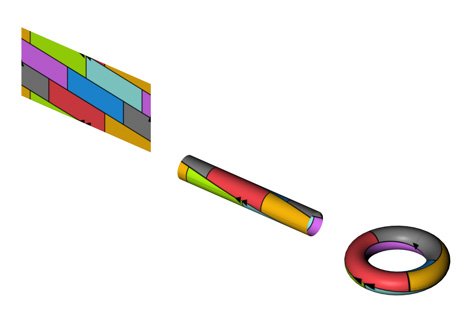
\includegraphics[width=0.8\textwidth]{media/Projection_color_torus.jpg}
	\\ \scriptsize Image from \cite{img:torus}
\end{center}

The torus can be realized as a CW complex with
\begin{itemize}
	\ii A $0$-skeleton consisting of a single point,
	\ii A $1$-skeleton consisting of two $1$-cells $e^1_a$, $e^1_b$, and
	\begin{center}
		\begin{asy}
			unitsize(1cm);
			draw(shift(-1,0)*unitcircle, blue, MidArrow);
			draw(shift(1,0)*rotate(180)*unitcircle, red, MidArrow);
			label("$e^1_a$", 2*dir(180), dir(180), blue);
			label("$e^1_b$", 2*dir(0), dir(0), red);
			dotfactor *= 1.4;
			dot("$e^0$", origin, dir(0));
		\end{asy}
	\end{center}
	\ii A $2$-skeleton with a single $2$-cell $e^2$,
	whose circumference is divided into four parts,
	and welded onto the $1$-skeleton ``via $aba\inv b \inv$''.
	This means: wrap a quarter of the circumference around $e^1_a$,
	then another quarter around $e^1_b$,
	then the third quarter around $e^1_a$ but in the opposite direction,
	and the fourth quarter around $e^1_b$ again in the opposite direction as before.
	\begin{center}
		\begin{asy}
			size(3cm);
			fill(unitcircle, yellow+opacity(0.2));
			defaultpen(linewidth(1));
			draw(arc(origin, 1, 45, 135), blue, MidArrow);
			draw(arc(origin, 1, 315, 225), blue, MidArrow);
			draw(arc(origin, 1, 135, 225), red, MidArrow);
			draw(arc(origin, 1, 45, -45), red, MidArrow);
			label("$e^2$", origin, origin);
		\end{asy}
	\end{center}
\end{itemize}
We say that $aba\inv b\inv$ is the \vocab{attaching word};
this shorthand will be convenient later on.

\subsection*{The Klein bottle}
The \vocab{Klein bottle} is defined similarly to
the torus, except one pair of edges is identified in the opposite manner,
as shown.

\begin{center}
	\begin{asy}
		size(2cm);
		fill(unitsquare, yellow+opacity(0.2));
		pair C = (0,0);
		pair B = (1,0);
		pair A = (1,1);
		pair D = (0,1);
		draw(A--B, red, MidArrow);
		draw(C--B, blue, MidArrow);
		draw(D--C, red, MidArrow);
		draw(A--D, blue, MidArrow);
	\end{asy}
\end{center}

Unlike the torus one cannot realize this in $3$-space
without self-intersecting. One can tape together the red edges
as before to get a cylinder, but to then fuse the resulting blue
circles in opposite directions is not possible in 3D.
Nevertheless, we often draw a picture in 3-dimensional space
in which we tacitly allow the cylinder to intersect itself.

\begin{center}
	\begin{minipage}[c]{0.5\textwidth}
	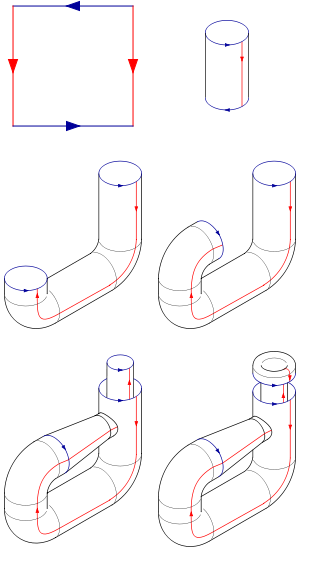
\includegraphics[width=\textwidth]{media/klein-fold.png}
	\end{minipage}
	\quad
	\begin{minipage}[c]{0.3\textwidth}
	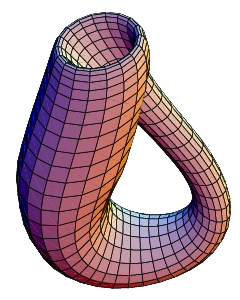
\includegraphics[width=\textwidth]{media/KleinBottle-01.png}
	\end{minipage}

	\scriptsize Image from \cite{img:kleinfold,img:kleinbottle}
\end{center}


Like the torus, the Klein bottle is realized as a CW complex with
\begin{itemize}
	\ii One $0$-cell,
	\ii Two $1$-cells $e^1_a$ and $e^1_b$, and
	\ii A single $2$-cell attached this time via the word $abab\inv$.
\end{itemize}

\subsection*{Real projective space}
Let's start with $n=2$.
The space $\RP^2$ is obtained if we reverse both directions of
the square from before, as shown.

\begin{center}
	\begin{asy}
		size(2cm);
		fill(unitsquare, yellow+opacity(0.2));
		pair C = (0,0);
		pair B = (1,0);
		pair A = (1,1);
		pair D = (0,1);
		draw(B--A, red, MidArrow);
		draw(C--B, blue, MidArrow);
		draw(D--C, red, MidArrow);
		draw(A--D, blue, MidArrow);
	\end{asy}
\end{center}

However, once we do this the fact that the original
polygon is a square is kind of irrelevant;
we can combine a red and blue edge to get the single purple edge.
Equivalently, one can think of this as a circle with half
its circumference identified with the other half:

\begin{center}
	\begin{asy}
		size(3cm);
		dotfactor *= 2;
		fill(unitcircle, opacity(0.2)+yellow);
		draw(dir(-90)..dir(0)..dir(90), purple, MidArrow);
		draw(dir(90)..dir(180)..dir(-90), purple, MidArrow);
		dot(dir(90));
		dot(dir(-90));
		label("$\mathbb{RP}^2$", origin, origin);
	\end{asy}
	\qquad
	\begin{asy}
		size(3cm);
		dotfactor *= 2;
		draw(dir(-90)..dir(0)..dir(90));
		draw(dir(90)..dir(180)..dir(-90), dashed);
		fill(unitcircle, yellow+opacity(0.2));
		dot(dir(90));
		opendot(dir(-90));
		label("$\mathbb{RP}^2$", origin, origin);
	\end{asy}
\end{center}

The resulting space should be familiar to those of you who do
projective (Euclidean) geometry.
Indeed, there are several possible geometric interpretations:
\begin{itemize}
	\ii One can think of $\RP^2$ as the set of lines through the
	origin in $\RR^3$, with each line being a point in $\RP^2$.

	Of course, we can identify each line with a point on the unit sphere $S^2$,
	except for the property that two antipodal points actually 
	correspond to the same line, so that $\RP^2$ can be almost thought
	of as ``half a sphere''. Flattening it gives the picture above.

	\ii Imagine $\RR^2$, except augmented with ``points at infinity''.
	This means that we add some points ``infinitely far away'',
	one for each possible direction of a line.
	Thus in $\RP^2$, any two lines indeed intersect
	(at a Euclidean point if they are not parallel, and at a point
	at infinity if they do).

	This gives an interpretation of $\RP^2$,
	where the boundary represents the \emph{line at infinity}
	through all of the points at infinity.
	Here we have used the fact that $\RR^2$
	and interior of $D^2$ are homeomorphic.
\end{itemize}
\begin{exercise}
	Observe that these formulations are equivalent
	by considering the plane $z=1$ in $\RR^3$,
	and intersecting each line in the first formulation with this plane.
\end{exercise}

We can also express $\RP^2$ using coordinates:
it is the set of triples $(x : y : z)$ of real numbers not all zero
up to scaling, meaning that 
\[ (x : y : z) = (\lambda x : \lambda y : \lambda z) \]
for any $\lambda \neq 0$.
Using the ``lines through the origin in $\RR^3$'' interpretation
makes it clear why this coordinate system gives the right space.
The points at infinity are those with $z = 0$,
and any point with $z \neq 0$ gives a Cartesian point since
\[ (x : y : z) = \left( \frac xz : \frac yz : 1 \right) \]
hence we can think of it as the Cartesian point $(\frac xz, \frac yz)$.

In this way we can actually define \vocab{real-projective $n$-space},
$\RP^n$ for any $n$, as either
\begin{enumerate}[(i)]
	\ii The set of lines through the origin in $\RR^{n+1}$,
	\ii Using $n+1$ coordinates as above, or
	\ii As $\RR^n$ augmented with points at infinity,
	which themselves form a copy of $\RP^{n-1}$.
\end{enumerate}

As a possibly helpful example, we give all three pictures of $\RP^1$.
\begin{example}
	[Real projective $1$-Space]
	$\RP^1$ can be thought of as $S^1$ modulo the relation
	the antipodal points are identified.
	Projecting onto a tangent line, we see that we get
	a copy of $\RR$ plus a single point at infinity, corresponding
	to the parallel line (drawn in cyan below).
	\begin{center}
		\begin{asy}
			size(7cm);
			filldraw(unitcircle, lightblue+opacity(0.2), heavyblue+opacity(0.4));
			label("$S^1$", dir(225), dir(225), lightblue);
			dot("$\vec 0$", origin, dir(45));
			pair X1 = (-2.1,1);
			pair X2 = (1.9,1);
			draw(X1--X2, heavyred, Arrows);
			dot("$0$", (0,1), dir(90), heavyred);
			dot("$1$", (1,1), dir(90), heavyred);
			pair P = extension( (0,1), (1,1), dir(250), dir(70) );
			dot("$0.36$", P, dir(90), heavyred);
			label("$\mathbb R$", X2, dir(105), heavyred);
			draw(L(dir(130),-dir(130),0.2,0.2), gray);
			draw(L(dir(250),-dir(250),0.2,0.2), gray);
			draw(L(dir(-20),-dir(-20),0.2,0.2), gray);
			draw(L(dir(0), -dir(0), 0.4,0.4), heavycyan+1);
		\end{asy}
	\end{center}

	Thus, the points of $\RP^1$ have two forms:
	\begin{itemize}
		\ii $(x:1)$, which we think of as $x \in \RR$ (in dark red above), and
		\ii $(1:0)$, which we think of as $1/0 = \infty$,
		corresponding to the cyan line above.
	\end{itemize}
	So, we can literally write
	\[ \RP^1 = \RR \cup \{\infty\}. \]
	Note that $\RP^1$ is also the boundary of $\RP^2$.
	In fact, note also that topologically we have
	\[ \RP^1 \cong S^1 \]
	since it is the ``real line with endpoints fused together''.
	\begin{center}
		\begin{asy}
			size(2cm);
			draw(unitcircle, heavyred);
			dot("$\infty$", dir(90), dir(90), heavycyan);
			dot("$0$", dir(-90), dir(-90), heavyred);
		\end{asy}
	\end{center}
\end{example}

Since $\RP^n$ is just ``$\RR^n$ (or $D^n$) with $\RP^{n-1}$ as its boundary'',
we can construct $\RP^n$ as a CW complex inductively.
Note that $\RP^n$ thus consists of \textbf{one cell in each dimension}.

\begin{example}[$\RP^n$ as a cell complex]
	\listhack
	\begin{enumerate}[(a)]
		\ii $\RP^0$ is a single point.
		\ii $\RP^1 \cong S^1$ is a circle, which as a CW complex
		is a $0$-cell plus a $1$-cell.
		\ii $\RP^2$ can be formed by taking a $2$-cell
		and wrapping its perimeter twice around a copy of $\RP^1$.
	\end{enumerate}
\end{example}

\subsection*{Complex projective space}
The \vocab{complex projective space} $\CP^n$ is
defined like $\RP^n$ with coordinates, i.e.\
\[ (z_0 : z_1 : \dots : z_n) \]
under scaling; this time $z_i$ are complex.
As before, $\CP^n$ can be thought of as $\CC^n$ augmented
with some points at infinity (corresponding to $\CP^{n-1}$).
\begin{example}
	[Complex projective space]
	\listhack
	\begin{enumerate}[(a)]
		\ii $\CP^0$ is a single point.
		\ii $\CP^1$ is $\CC$ plus a single point at infinity
		(``complex infinity'' if you will).
		That means as before we can think of $\CP^1$ as
		\[ \CP^1 = \CC \cup \{\infty\}. \]
		So, imagine taking the complex plane and then adding
		a single point to encompass the entire boundary.
		The result is just sphere $S^2$.
	\end{enumerate}
	Here is a picture of $\CP^1$ with its coordinate system,
	the \vocab{Riemann sphere}.
	\begin{center}
		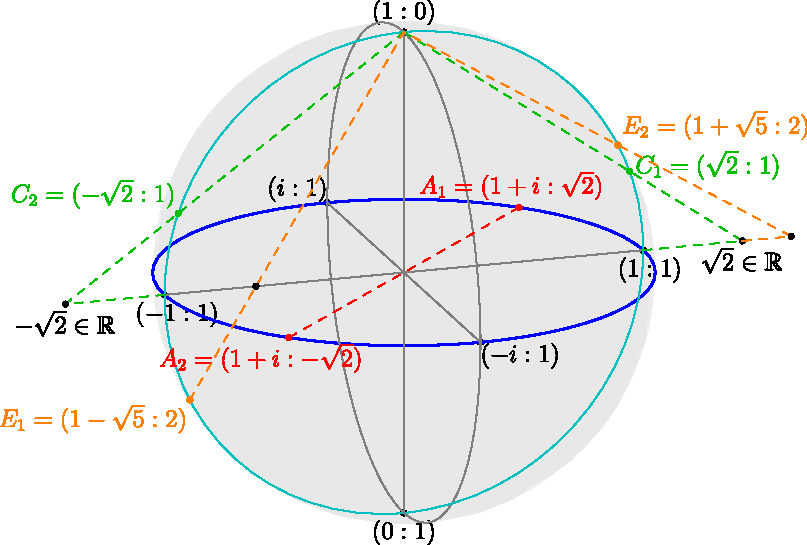
\includegraphics[width=0.9\textwidth]{media/earth.pdf}
	\end{center}
\end{example}

\begin{remark}
	[For Euclidean geometers]
	You may recognize that while $\RP^2$ is the setting for projective geometry,
	inversion about a circle is done in $\CP^1$ instead.
	When one does an inversion sending generalized circles to generalized
	circles, there is only one point at infinity:
	this is why we work in $\CP^n$.
\end{remark}

Like $\RP^n$, $\CP^n$ is a CW complex, built inductively
by taking $\CC^n$ and welding its boundary onto $\CP^{n-1}$
The difference is that as topological spaces,
\[ \CC^n \cong \RR^{2n} \cong D^{2n}. \]
Thus, we attach the cells $D^0$, $D^2$, $D^4$ and so on
inductively to construct $\CP^n$.
Thus we see that
\begin{moral}
	$\CP^n$ consists of one cell in each \emph{even} dimension.
\end{moral}


\section\problemhead
\begin{problem}
	Show that a space $X$ is Hausdorff if and only if the diagonal
	$\{(x,x) \mid x \in X\}$ is closed in the product space $X \times X$.
\end{problem}
\begin{problem}
	Realize the following spaces as CW complexes:
	\begin{enumerate}[(a)]
		\ii M\"obius strip.
		\ii $\RR$.
		\ii $\RR^n$.
	\end{enumerate}
\end{problem}
\begin{dproblem}
	Show that a finite CW complex is compact.
	\begin{hint}
		Prove and use the fact that a quotients of compact spaces remain compact.
	\end{hint}
\end{dproblem}
 
\chapter{Fundamental groups}
Topologists can't tell the difference between a coffee cup and a doughnut.
So how do you tell \emph{anything} apart?

This is a very hard question to answer, but one way we can
try to answer it is to find some \emph{invariants} of the space.
To draw on the group analogy, two groups are clearly not isomorphic if,
say, they have different orders, or if one is simple and the other isn't, etc.
We'd like to find some similar properties for topological spaces
so that we can actually tell them apart.

Two such invariants for a space $X$ are
\begin{itemize}
	\ii Defining homology groups $H_1(X)$, $H_2(X)$, \dots
	\ii Defining homotopy groups $\pi_1(X)$, $\pi_2(X)$, \dots
\end{itemize}
Homology groups are hard to define, but in general easier to compute.
Homotopy groups are easier to define but harder to compute.

This chapter is about the fundamental group $\pi_1$.


\section{Fusing paths together}
Recall that a \emph{path} in a space $X$ is a function $[0,1] \to X$.
Suppose we have paths $\gamma_1$ and $\gamma_2$
such that $\gamma_1(1) = \gamma_2(0)$.
We'd like to fuse\footnote{%
	Almost everyone else in the world uses ``gluing'' to describe this
	and other types of constructs.
	But I was traumatized by Elmer's glue when I was a in high school
	because I hated the stupid ``make a poster'' projects and hated
	having to use glue on them.
	So I refuse to talk about ``gluing'' paths together, referring
	instead to ``fusing'' them together, which sounds cooler anyways.
} them together to get a path $\gamma_1 \ast \gamma_2$.  Easy, right?

\begin{center}
	\begin{asy}
		size(8cm);
		bigblob("$X$");
		pair A = Drawing("\gamma_1(0)", (-3,-1));
		pair B = Drawing("\gamma_1(1) = \gamma_2(0)", (1,1), dir(90));
		pair C = Drawing("\gamma_2(1)", (2,-2), dir(-90));
		path p = A..(-2,0)..(0,0.5)..B;
		path q = B..(1.8,-0.5)..C;
		draw(p, red, EndArrow);
		draw(q, blue, EndArrow);
		MP("\gamma_1", midpoint(p), dir(90));
		MP("\gamma_2", midpoint(q), dir(0));
	\end{asy}
\end{center}

We unfortunately do have to hack the definition a tiny bit. In an ideal world, we'd have a path $\gamma_1 : [0,1] \to X$ and $\gamma_2 : [1,2] \to X$ and we could just merge them together to get $\gamma_1 \ast \gamma_2 : [0,2] \to X$.
But the ``$2$'' is wrong here.
The solution is that we allocate $[0, \half]$ for the first path
and $[\half, 1]$ for the second path; we run ``twice as fast''.

\begin{definition}
	Given two paths $\gamma_1, \gamma_2 : [0,1] \to X$
	such that $\gamma_1(1) = \gamma_2(0)$, we define
	a path $\gamma_1 \ast \gamma_2 : [0,1] \to X$ by
	\[ 
		(\gamma_1 \ast \gamma_2)(t)
		=
		\begin{cases}
			\gamma_1(2t) & 0 \le t \le \half \\
			\gamma_2(2t-1) & \half \le t \le 1.
		\end{cases}
		\]
\end{definition}

This hack unfortunately reveals a second shortcoming: this ``product'' is not associative.
If we take $(\gamma_1 \ast \gamma_2) \ast \gamma_3$ for some suitable paths,
then $[0, \frac14]$, $[\frac14, \frac12]$ and $[\frac12, 1]$
are the times allocated for $\gamma_1$, $\gamma_2$, $\gamma_3$.
\begin{ques}
	What are the times allocated
	for $\gamma_1 \ast (\gamma_2 \ast \gamma_3)$?
\end{ques}
But I hope you'll agree that even though this operation isn't associative,
the reason it fails to be associative is kind of stupid.
It's just a matter of how fast we run in certain parts.

\begin{center}
	\begin{asy}
		unitsize(6cm);
		D( unitsquare);
		MP("0", (0,0), S);
		MP("1", (1,0), S);
		MP("\frac{1}{4}", (1/4, 0), S);
		MP("\frac{1}{2}", (1/2, 0), S);
		MP("0", (0,1), N);
		MP("1", (1,1), N);
		MP("\frac{3}{4}", (3/4, 1), N);
		MP("\frac{1}{2}", (1/2, 1), N);
		MP("\gamma_1", (1/8, 0), N);
		MP("\gamma_2", (3/8, 0), N);
		MP("\gamma_3", (3/4, 0), N);
		MP("\gamma_1", (1/4, 1), S);
		MP("\gamma_2", (5/8, 1), S);
		MP("\gamma_3", (7/8, 1), S);

		MP("\boxed{\gamma_1 \ast \left( \gamma_2 \ast \gamma_3 \right)}", (0.5,1.2), origin);
		MP("\boxed{\left( \gamma_1 \ast \gamma_2 \right) \ast \gamma_3}", (0.5,-0.2), origin);

		D((1/4,0)--(1/2,1), blue);
		D((1/2,0)--(3/4,1), blue);
		D( (1/2,0)--(1/2,1), dotted);
	\end{asy}
\end{center}

So as long as we're fusing paths together,
we probably don't want to think of $[0,1]$ itself too seriously.
And so we only consider everything up to (path) homotopy equivalence.
(Recall that two paths $\alpha$ and $\beta$ are homotopic if
there's a path homotopy $F : [0,1]^2 \to X$ between them,
which is a continuous deformation from $\alpha$ to $\beta$.)
It is definitely true that
\[
	\left( \gamma_1 \ast \gamma_2 \right) \ast \gamma_3
	\simeq 
	\gamma_1 \ast \left( \gamma_2 \ast \gamma_3 \right) . \]
It is also true that if $\alpha_1 \simeq \alpha_2$ and $\beta_1 \simeq \beta_2$
then $\alpha_1 \ast \beta_1 \simeq \alpha_2 \ast \beta_2$.

Naturally, homotopy is an equivalence relation,
so paths $\gamma$ lives in some ``homotopy type'',
the equivalence classes under $\simeq$. We'll denote this $[\gamma]$.
Then it makes sense to talk about $[\alpha] \ast [\beta]$.
Thus, \textbf{we can think of $\ast$ as an operation on homotopy classes}.


\section{Fundamental groups}
\prototype{$\pi_1(\RR^2)$ is trivial and $\pi_1(S^1) \cong \ZZ$.}

At this point I'm a little annoyed at keeping track of endpoints,
so now I'm going to specialize to a certain type of path.
\begin{definition}
	A \vocab{loop} is a path with $\gamma(0) = \gamma(1)$.
\end{definition}
\begin{center}
	\begin{asy}
		bigblob("$X$");
		pair A = Drawing("x_0", (-1,0), dir(100));
		path p = A..(1,1)..(2,0)..(0.5,-1)..(-1.5,-0.5)..cycle;
		draw(p, blue, EndArrow);
		MP("\gamma", midpoint(p), dir(-20));
	\end{asy}
\end{center}

Hence if we restrict our attention to paths starting at a single point $x_0$,
then we can stop caring about endpoints and start-points, since
everything starts and stops at $x_0$.
We even have a very canonical loop: the ``do-nothing'' loop\footnote{Fatty.} given by standing at $x_0$ the whole time.

\begin{definition}
	Denote the trivial ``do-nothing loop'' by $1$.
	A loop $\gamma$ is \vocab{nulhomotopic} if it is homotopic to $1$; i.e.\ $\gamma \simeq 1$.
\end{definition}

For homotopy of loops, you might visualize ``reeling in'' the loop, contracting it to a single point.

\begin{example}[Loops in $S^2$ are nulhomotopic]
	As the following picture should convince you, every loop in
	the simply connected space $S^2$ is nulhomotopic.
	\begin{center}
		\includegraphics{media/S2-simply-connect.pdf}
	\end{center}
	(Starting with the purple loop, we contract to the red-brown point.)
\end{example}

Hence to show that spaces are simply connected it suffices to understand
the loops of that space.
We are now ready to provide:
\begin{definition}
	The \vocab{fundamental group} of $X$ with basepoint $x_0$,
	denoted $\pi_1(X, x_0)$, is the set of homotopy classes
	\[ \left\{ [\gamma] \mid \gamma \text{ a loop at $x_0$} \right\} \]
	equipped with $\ast$ as a group operation.
\end{definition}

It might come as a surprise that this has a group structure.
For example, what is the inverse?
Let's define it now.
\begin{definition}
	Given a path $\alpha : [0,1] \to X$ we can define a path $\ol\alpha$
	\[ \ol\alpha (t) = \alpha(1-t). \]
	In effect, this ``runs $\alpha$ backwards''.
	Note that $\ol\alpha$ starts at the endpoint of $\alpha$
	and ends at the starting point of $\alpha$.
\end{definition}
\begin{exercise}
	Show that for any path $\alpha$,
	$\alpha \ast \ol\alpha$ is homotopic
	to the ``do-nothing'' loop at $\alpha(0)$.
	(Draw a picture.)
\end{exercise}

Let's check it.
\begin{proof}
	[Proof that this is a group structure]
	Clearly $\ast$ takes two loops at $x_0$ and spits out a loop at $x_0$.
	We also already took the time to show that $\ast$ is associative.
	So we only have to check that (i) there's an identity, and (ii)
	there's an inverse.
	\begin{itemize}
		\ii We claim that the identity is the ``do-nothing'' loop $1$
		we described above. The reader can check that for any $\gamma$,
		\[ \gamma \simeq \gamma \ast 1 = 1 \ast \gamma. \]
		\ii For a loop $\gamma$, recall again we define its ``backwards'' loop $\ol\gamma$ by
		\[ \ol\gamma(t) = \gamma(1-t). \]
		Then we have $\gamma \ast \ol\gamma = \ol\gamma \ast \gamma = 1$.
	\end{itemize}
	Hence $\pi_1(X,x_0)$ is actually a group.
\end{proof}

Before going any further I had better give some examples.
\begin{example}
	[Examples of fundamental groups]
	Note that proving the following results is not at all trivial.
	For now, just try to see intuitively why the claimed answer ``should'' be correct.
	\begin{enumerate}[(a)]
		\ii The fundamental group of $\CC$ is the
		trivial group: in the plane, every loop is nulhomotopic.
		(Proof: imagine it's a piece of rope and reel it in.)
		\ii On the other hand, the fundamental group of $\CC - \{0\}$
		(meteor example from earlier) with any base point is actually $\ZZ$!
		We won't be able to prove this for a while,
		but essentially a loop is determined by the number of times
		that it winds around the origin -- these are so-called
		\emph{winding numbers}.  Think about it!
		\ii Similarly, we will soon show that the fundamental group of $S^1$
		(the boundary of the unit circle) is $\ZZ$.
	\end{enumerate}
	Officially, I also have to tell you what the base point is, but
	by symmetry in these examples, it doesn't matter.
\end{example}
Here is the picture for $\CC \setminus \{0\}$, with the hole exaggerated
as the meteor from last chapter.
\begin{center}
	\begin{asy}
		size(6cm);
		bigbox("$\mathbb C \setminus \{0\}$");
		filldraw(scale(0.5)*unitcircle, grey, black);
		dot("$x_0$", (1.4,0), dir(0));
		draw( (1.4,0)..(0,1.4)..(-1.4,0)..(1.4*dir(-30))..cycle, blue, EndArrow );
	\end{asy}
\end{center}

\begin{ques}
	Convince yourself that the fundamental group of $S^1$ is $\ZZ$,
	and understand why we call these ``winding numbers''.
	(This will be the most important example of a fundamental group
	in later chapters, so it's crucial you figure it out now.)
\end{ques}

\begin{example}
	[The figure eight]
	\label{ex:figure8}
	Consider a figure eight $S^1 \vee S^1$, and let $x_0$
	be the center.
	Then  \[\pi_1(S^1 \vee S^1, x_0) \cong \left<a,b\right> \]
	is the \emph{free group} generated on two letters.
	The idea is that one loop of the eight is $a$,
	and the other loop is $b$, so we expect $\pi_1$
	to be generated by this loop $a$ and $b$ (and its inverses
	$\ol a$ and $\ol b$).
	These loops don't talk to each other.
	\begin{center}
		\begin{asy}
			draw( shift( (1,0) ) * unitcircle, grey + 5 );
			draw( shift( (-1,0) ) * unitcircle, grey + 5 );
			dot(origin);
			path g = dir(20)..dir(100)..dir(180)..dir(260)..dir(340);
			draw( shift( (1,0) ) * scale(0.8) * reflect(dir(90),dir(-90)) * g, blue, EndArrow );
			draw( shift( (-1,0) ) * scale(0.8) * g, red, EndArrow );
			label("$a$", (-1.6,0), dir(0));
			label("$b$", (1.6,0), dir(180));
		\end{asy}
	\end{center}
\end{example}

Recall that in graph theory, we usually assume our graphs are connected,
since otherwise we can just consider every connected component separately.
Likewise, we generally want to restrict our attention to path-connected spaces, since if a space isn't path-connected then it can be broken into a bunch of ``path-connected components''.
(Can you guess how to define this?)
Indeed, you could imagine a space $X$ that consists of the objects on my desk (but not the desk itself): $\pi_1$ of my phone has nothing to do with $\pi_1$ of my mug. They are just totally disconnected, both figuratively and literally.

But on the other hand we claim that in a path-connected space,
the groups are very related!
\begin{theorem}[Fundamental groups don't depend on basepoint]
	Let $X$ be a path-connected space.
	Then for any $x_1 \in X$ and $x_2 \in X$, we have
	\[ \pi_1(X, x_1) \cong \pi_1(X, x_2). \]
\end{theorem}
Before you read the proof, see if you can guess the isomorphism based just on the picture below.
\begin{center}
	\begin{asy}
		size(7cm);
		bigblob("$X$");
		pair A = Drawing("x_1", (-1.5,0), dir(180));
		pair B = Drawing("x_2", (1.5,0), dir(0));
		draw(A..(-2.5,-0.8)..(-2.5,0.9)..cycle, blue);
		draw(B..(2.2,-1.1)..(2.4,0.8)..cycle, blue);
		draw(A--B, red+dashed, Arrows);
		label("$\alpha$/$\overline{\alpha}$", origin, dir(90));
	\end{asy}
\end{center}
\begin{proof}
	Let $\alpha$ be any path from $x_1$ to $x_2$ (possible by path-connectedness), and let $\ol\alpha$ be its reverse.
	Then we can construct a map
	\[ 
		\pi_1(X,x_1) \to \pi_1(X,x_2)
		\text{ by }
		[\gamma] \mapsto [\ol\alpha \ast \gamma \ast \alpha]. \]
	In other words, given a loop $\gamma$ at $x_1$,
	we can start at $x_2$, follow $\ol\alpha$ to $x_1$,
	run $\gamma$, then run along $\alpha$ home to $x_2$.
	Hence this is a map which builds a loop of $\pi_1(X, x_2)$
	from every loop at $\pi_1(X, x_1)$.
	It is a \emph{homomorphism} of the groups just because
	\[ \left( \ol \alpha \ast \gamma_1 \ast \alpha \right)
		\ast \left( \ol\alpha \ast \gamma_2 \ast \alpha \right)
		= \ol\alpha \ast \gamma_1 \ast \gamma_2 \ast \alpha \]
	as $\alpha \ast \ol\alpha$ is nulhomotopic.

	Similarly, there is a homomorphism
	\[ 
		\pi_1(X,x_2) \to \pi_1(X,x_1)
		\text{ by }
		[\gamma] \mapsto [\alpha \ast \gamma \ast \ol\alpha]. \]
	As these maps are mutual inverses, it follows
	they must be isomorphisms. End of story.
\end{proof}
This is a bigger reason why we usually only care about path-connected spaces.

\begin{abuse}
	For a path-connected space $X$ we will often abbreviate $\pi_1(X, x_0)$
	to just $\pi_1(X)$, since it doesn't matter which $x_0 \in X$
	we pick.
\end{abuse}

Finally, recall that we originally defined ``simply connected'' as saying
that any two paths with matching endpoints were homotopic.
It's possible to weaken this condition and then rephrase it using
fundamental groups.
\begin{exercise}
	Let $X$ be a path-connected space.
	Prove that $X$ is \vocab{simply connected} if and only if
	$\pi_1(X)$ is the trivial group.
	(One direction is easy; the other is a little trickier.)
\end{exercise}
This is the ``usual'' definition of simply connected.


\section{Fundamental groups are functorial}
One quick shorthand I will introduce to clean up the discussion:
\begin{definition}
	By $f : (X, x_0) \to (Y, y_0)$, we will mean that
	$f : X \to Y$ is a continuous function of spaces
	which also sends the point $x_0$ to $y_0$.
\end{definition}

Let $X$ and $Y$ be topological spaces and $f : (X, x_0) \to (Y, y_0)$.
We now want to relate the fundamental groups of $X$ and $Y$.

Recall that a loop $\gamma$ in $(X, x_0)$ is a map $\gamma : [0,1] \to X$
with $\gamma(0) = \gamma(1) = x_0$.
Then if we consider the composition
\[ [0,1] \taking\gamma (X, x_0) \taking f (Y, y_0) \]
then we get straight-away a loop in $Y$ at $y_0$!
Let's call this loop $f_\sharp \gamma$.
\begin{lemma}[$f_\sharp$ is homotopy invariant]
	\label{lem:fsharp_homotopy_invariant}
	If $\gamma_1 \simeq \gamma_2$ are path-homotopic,
	then in fact
	\[ f_\sharp \gamma_1 \simeq f_\sharp \gamma_2. \]
\end{lemma}
\begin{proof}
	Just take the homotopy $h$ taking $\gamma_1$ to $\gamma_2$	
	and consider $f \circ h$.
\end{proof}

It's worth noting at this point that if $X$ and $Y$ are homeomorphic,
then their fundamental groups are all isomorphic.
Indeed, let $f : X \to Y$ and $g : Y \to X$ be mutually inverse continuous maps.
Then one can check that $f_\sharp : \pi_1(X, x_0) \to \pi_1(Y, y_0)$
and $g_\sharp : \pi_1(Y, y_0) \to \pi_1(X, x_0)$ are inverse maps
between the groups (assuming $f(x_0) = y_0$ and $g(y_0) = x_0$).

%Now we want to show that by taking the map $f_\sharp$, we get a \emph{functor}
%\begin{diagram}
%	& (X, x_0) & & \pi_1(X, x_0) & \\
%	\catname{Top}_\ast \ni & \dTo^f & \rDotted & \dTo_{f_\sharp} & \in \catname{Gp} \\
%	& (Y, y_0) & & \pi_1(Y, y_0) &
%\end{diagram}
%\begin{ques}
%	Check this -- we need that $(f \circ g)_\sharp = f_\sharp \circ g_\sharp$
%	and that $(\id_X)_\sharp = \id_{\pi_1(X)}$.
%	Both are totally obvious once you can tell what they're asking.
%\end{ques}
%Thus in this way we've constructed a functor
%\[ \catname{Top}_\ast \to \catname{Gp}. \]
%In particular, by the fact that functors preserve isomorphism (\Cref{thm:functor_isom}), we have
%\begin{moral}
%	Homeomorophic topological spaces have isomorphic fundamental groups.
%	Category theory gives this to us for free.
%\end{moral}
%
%\begin{remark}
%	Note the similarity between this and the construction
%	of the covariant Yoneda functor (\Cref{ex:covariant_yoneda}).
%\end{remark}

\section{Higher homotopy groups}
Why the notation $\pi_1$ for the fundamental group?
And what are $\pi_2$, \dots?
The answer lies in the following rephrasing:
\begin{ques}
	Convince yourself that a loop is the same thing
	as a continuous function $S^1 \to X$.
\end{ques}
It turns out we can define homotopy for things other than paths.
Two functions $f, g : Y \to X$ are \vocab{homotopic} if there exists a continuous
function $Y \times [0,1] \to X$ which continuously deforms $f$ to $g$.
So everything we did above was just the special case $Y = S^1$.

For general $n$, the group $\pi_n(X)$ is defined as the homotopy classes
of the maps $S^n \to X$.
The group operation is a little harder to specify.
You have to show that $S^n$ is homeomorphic to $[0,1]^n$ with
some endpoints fused together; for example $S^1$ is $[0,1]$ with $0$ fused to $1$.
Once you have these cubes, you can merge them together on a face.
(Again, I'm being terribly imprecise, deliberately.)

For $n \neq 1$, $\pi_n$ behaves somewhat differently than $\pi_1$.
(You might not be surprised, as $S^n$ is simply connected for all $n \ge 2$ but not when $n=1$.)
In particular, it turns out that $\pi_n(X)$ is an abelian group for all $n \ge 2$.

Let's see some examples.
\begin{example}[$\pi_n(S^n) \cong \mathbb Z$]
	As we saw, $\pi_1(S^1) \cong \ZZ$; given the base circle $S^1$,
	we can wrap a second circle around it as many times as we want.
	In general, it's true that $\pi_n(S^n) \cong \ZZ$.
\end{example}
\begin{example}[$\pi_n(S^m) \cong \{1\}$ when $n < m$]
	We saw that $\pi_1(S^2) \cong \{1\}$, because 
	a circle in $S^2$ can just be reeled in to a point.
	It turns out that similarly, any smaller $n$-dimensional sphere
	can be reeled in on the surface of a bigger $m$-dimensional sphere.
	So in general, $\pi_n(S^m)$ is trivial for $n < m$.
\end{example}
However, beyond these observations, the groups behave quite weirdly.
Here is a table of $\pi_n(S^m)$ for some values of $m$ and $n$
taken from Wikipedia.

\[
	\begin{array}{r|rccccccccc}
		\pi_n(S^m) & m = 1 & 2 & 3 & 4 & 5 & 6 & 7 & 8 & 9 & 10 \\ \hline
		n = 1 & \ZZ & \{1\} & \{1\} & \{1\} & \{1\} & \{1\} & \{1\} & \{1\} & \{1\} & \{1\} \\
		2 &  & \ZZ & \ZZ & \Zc2 & \Zc2 & \Zc{12} & \Zc2 & \Zc2 & \Zc3 & \Zc{15}\\
		3 &  &  & \ZZ & \Zc2 & \Zc2 & \Zc{12} & \Zc2 & \Zc2 & \Zc3 & \Zc{15}\\
		4 &  &  &  & \ZZ & \Zc2 & \Zc2 & \ZZ \times \Zc{12} & \Zc2^2 & \Zc2 \times \Zc2 & \Zc{24} \times \Zc3 \\
		5 &  &  &  &  & \ZZ & \Zc2 & \Zc2 & \Zc{24} & \Zc2 & \Zc2 \\
		6 &  &  &  &  &  & \ZZ & \Zc2 & \Zc2 & \Zc{24} & \{1\} \\
		7 &  &  &  &  &  &  & \ZZ & \Zc2 & \Zc2 & \Zc{24} \\
		8 &  &  &  &  &  &  &  & \ZZ & \Zc2 & \Zc2
	\end{array}
\]

Actually, it turns out that if you can compute $\pi_n(S^m)$
for every $m$ and $n$,
then you can essentially compute \emph{any} homotopy classes.
Thus, computing $\pi_n(S^m)$ is sort of a lost cause in general,
and the mixture of chaos and pattern in the above table is a testament to this.

\section{Homotopy equivalent spaces}
\prototype{A disk is homotopy equivalent to a point, an annulus is homotopy equivalent to $S^1$.}
Up to now I've abused notation and referred to ``path homotopy'' as just ``homotopy'' for two paths.
I will unfortunately continue to do so (and so any time I say two paths are homotopic, you should assume I mean ``path-homotopic'').
But let me tell you what the general definition of homotopy is first.
\begin{definition}
	Let $f,g : X \to Y$ be continuous functions.
	A \vocab{homotopy} is a continuous function $F : X \times [0,1] \to Y$,
	which we'll write $F_s(x)$ for $s \in [0,1]$, $x \in X$, such that 
	\[ F_0(x) = f(x) \text{ and } F_1(x) = g(x) \text{ for all $x \in X$.} \]
	If such a function exists, then $f$ and $g$ are \vocab{homotopic}.
\end{definition}
Intuitively this is once again ``deforming $f$ to $g$''.
You might notice this is almost exactly the same definition as path-homotopy,
except that $f$ and $g$ are any functions instead of paths, and hence
there's no restriction on keeping some ``endpoints'' fixed through the deformation.

This homotopy can be quite dramatic:
\begin{example}
	The zero function $z \mapsto 0$ and the identity function $z \mapsto z$
	are homotopic as functions $\CC \to \CC$.
	The necessary deformation is
	\[ [0,1] \times \CC \to \CC \text{ by } (t,z) \mapsto tz. \]
\end{example}

I bring this up because I want to define:
\begin{definition}
	Let $X$ and $Y$ be continuous spaces.
	They are \vocab{homotopy equivalent} if there exist
	functions $f : X \to Y$ and $g : Y \to X$ such that
	\begin{enumerate}[(i)]
		\ii $f \circ g : X \to X$ is homotopic to the identity map on $X$, and
		\ii $g \circ f : Y \to Y$ is homotopic to the identity map on $Y$.
	\end{enumerate}
	If a topological space is homotopy equivalent to a point,
	then it is said to be \vocab{contractible}.
\end{definition}
\begin{ques}
	Why are two homeomorphic spaces also homotopy equivalent?
\end{ques}

Intuitively, you can think of this as a more generous form of stretching
and bending than homeomorphism: we are allowed to compress huge spaces into single points.

\begin{example}[$\CC$ is contractible]
	Consider the topological spaces $\CC$
	and the space consisting of the single point $\{0\}$. 
	We claim these spaces are homotopy equivalent (can you guess what $f$ and $g$ are?)
	Indeed, the two things to check are
	\begin{enumerate}[(i)]
		\ii $\CC \to \{0\} \hookrightarrow \CC$ by $z \mapsto 0 \mapsto 0$
		is homotopy equivalent to the identity on $\CC$, which we just saw, and
		\ii $\{0\} \hookrightarrow \CC \to \{0\}$ by $0 \mapsto 0 \mapsto 0$, which \emph{is} the identity on $\{0\}$.
	\end{enumerate}
	Here by $\hookrightarrow$ I just mean $\to$ in the special case
	that the function is just an ``inclusion''.
\end{example}
\begin{remark}
	$\CC$ cannot be \emph{homeomorphic} to a point
	because there is no bijection of sets between them.
\end{remark}

\begin{example}[$\CC \setminus \{0\}$ is homotopy equivalent to $S^1$]
	Consider the topological spaces $\CC \setminus \{0\}$,
	the \vocab{punctured plane}, and the circle $S^1$ viewed as a subset of $S^1$.
	We claim these spaces are actually homotopy equivalent!
	The necessary functions are the inclusion
	\[ S^1 \hookrightarrow \CC \setminus \{0\} \]
	and the function
	\[ \CC \setminus \{0\} \to S^1
		\quad\text{by}\quad
		z \mapsto \frac{z}{\left\lvert z \right\rvert}. \]
	You can check that these satisfy the required condition.
\end{example}
\begin{remark}
	On the other hand, $\CC \setminus \{0\}$ cannot be \emph{homeomorphic} to $S^1$.
	One can make $S^1$ disconnected by deleting two points;
	the same is not true for $\CC \setminus \{0\}$.
\end{remark}
\begin{example}
	[$\text{Disk} = \text{Point}$, $\text{Annulus} = \text{Circle}$.]
	By the same token, a disk is homotopic to a point;
	an annulus is homotopic to a circle.
	(This might be a little easier to visualize, since it's finite.)
\end{example}

I bring these up because it turns out that 
\begin{moral}
	Algebraic topology can't distinguish between homotopy equivalent spaces.
\end{moral}
More precisely,
\begin{theorem}[Homotopy equivalent spaces have isomorphic fundamental groups]
	\label{thm:fundgrp_homotopy_invariant}
	Let $X$ and $Y$ be path-connected, homotopy-equivalent spaces.
	Then $\pi_n(X) \cong \pi_n(Y)$ for every positive integer $n$.
\end{theorem}
\begin{proof}
	Let $\gamma : [0,1] \to X$ be a loop.
	Let $f : X \to Y$ and $g : Y \to X$ be maps witnessing that $X$ and $Y$ are homotopy equivalent
	(meaning $f \circ g$ and $g \circ f$ are each homotopic to the identity).
	Then the composition
	\[ [0,1] \taking\gamma X \taking f Y \]
	is a loop in $Y$ and hence $f$ induces a natural homomorphism $\pi_1(X) \to \pi_1(Y)$.
	Similarly $g$ induces a natural homomorphism $\pi_1(Y) \to \pi_1(X)$.
	The conditions on $f$ and $g$ now say exactly that these two homomorphisms
	are inverse to each other, meaning the maps are isomorphisms.
\end{proof}
In particular,
\begin{ques}
	What are the fundamental groups of contractible spaces?
\end{ques}

That means, for example, that algebraic topology can't tell
the following homotopic subspaces of $\RR^2$ apart.
\begin{center}
	{\color{red} \Huge \venus}
	\qquad
	{\color{blue} \Huge \mars}
\end{center}

\section{The pointed homotopy category}
This section is meant to be read by those who know some basic category theory.
Those of you that don't should come back after reading \Cref{ch:cats,ch:functors}.
Those of you that do will enjoy how succinctly, we can summarize
the content of this chapter using categorical notions.

\begin{definition}
	The \vocab{pointed homotopy category} $\catname{hTop}_\ast$ is defined as follows.
	\begin{itemize}
		\ii Objects: pairs $(X, x_0)$ of spaces with a distinguished basepoint, and
		\ii Morphisms: \emph{homotopy classes} of continuous functions $(X, x_0) \to (Y, y_0)$.
	\end{itemize}
\end{definition}
In particular, two path-connected spaces are isomorphic in this category exactly
when they are homotopy equivalent.
Then we can summarize many of the preceding results as follows:
\begin{theorem}[Functorial interpretation of fundamental groups]
	\label{thm:fundgrp_functor}
	There is a functor
	\[ \pi_1 : \catname{hTop}_\ast \to \catname{Gp} \]
	sending
	\begin{diagram}
		(X,x_0) & \rTo & \pi_1(X, x_0) \\
		\dTo^f & & \dTo^{f_\sharp} \\
		(Y,y_0) & \rTo & \pi_1(Y, y_0)
	\end{diagram}
\end{theorem}
This implies several things, like
\begin{itemize}
	\ii The functor bundles the information of $f_\sharp$,
	including the fact that it respects composition.
	In the categorical language, $f_\sharp$ is $\pi_1(f)$.
	\ii Homotopic spaces have isomorphic fundamental group
	(since the spaces are isomorphic in $\catname{hTop}$,
	and functors preserve isomorphism by \Cref{thm:functor_isom}).
	In fact, you'll notice that the proofs
	of \Cref{thm:functor_isom} and \Cref{thm:fundgrp_homotopy_invariant}
	are secretly identical to each other.
	\ii If maps $f, g : (X, x_0) \to (Y, y_0)$ are homotopic,
	then $f_\sharp = g_\sharp$. This is basically \Cref{lem:fsharp_homotopy_invariant}
\end{itemize}

\begin{remark}
	In fact, $\pi_1(X, x_0)$ is the set of arrows $(S^1, 1) \to (X, x_0)$ in $\catname{hTop}_\ast$,
	so this is actually a covariant Yoneda functor (\Cref{ex:covariant_yoneda}),
	except with target $\catname{Gp}$ instead of $\catname{Set}$.
\end{remark}


\section\problemhead

\begin{problem}[Harmonic fan]
	Exhibit a subspace $X$ of the metric space $\RR^2$ which is
	path-connected but for which a point $p$ can be found such that
	any $r$-neighborhood of $p$ with $r < 1$ is not path-connected.
	% harmonic fan
\end{problem}

\begin{dproblem}
	[Special case of Seifert-van Kampen] \gim
	Let $X$ be a topological space.
	Suppose $U$ and $V$ are connected open subsets of $X$, with $X = U \cup V$,
	so that $U \cap V$ is nonempty and path-connected.
		
	Prove that if $\pi_1(U) = \pi_1(V) = \{1\}$ then $\pi_1(X) = 1$.
\end{dproblem}
\begin{remark}
	The \vocab{Seifert--van Kampen theorem} generalizes this 
	for $\pi_1(U)$ and $\pi_1(V)$ any groups; it gives a formula for calculating $\pi_1(X)$
	in terms of $\pi_1(U)$, $\pi_1(V)$, $\pi_1(U \cap V)$.
	The proof is much the same.
	
	Unfortunately, this does not give us a way to calculate $\pi_1(S^1)$,
	because it is not possible to write $S^1 = U \cup V$ for $U \cap V$ \emph{connected}.
\end{remark}

\begin{problem}
	[RMM 2013] \yod
	Let $n \ge 2$ be a positive integer.
	A stone is placed at each vertex of a regular $2n$-gon.
	A move consists of selecting an edge of the $2n$-gon and swapping the two stones at the endpoints of the edge.
	Prove that if a sequence of moves swaps every pair of stones exactly once, then there is some edge never used in any move.
\end{problem}
(This last problem doesn't technically have anything to do with the chapter,
but the ``gut feeling'' which motivates the solution is very similar.)

\chapter{Covering projections}
A few chapters ago we talked about what a fundamental group was,
but we didn't actually show how to compute any of them
except for the most trivial case of a simply connected space.
In this chapter we'll introduce the notion of a \emph{covering projection},
which will let us see how some of these groups can be found.

\section{Even coverings and covering projections}
\prototype{$\RR$ covers $S^1$.}
What we want now is a notion where a big space $E$, a ``covering space'',
can be projected down onto a base space $B$ in a nice way.
Here is the notion of ``nice'':
\begin{definition}
	Let $p : E \to B$ be a continuous function.
	Let $U$ be an open set of $B$.
	We call $U$ \vocab{evenly covered} (by $p$) if $p\pre(U)$ is a disjoint union of open sets (possibly infinite) such that $p$ restricted to any of these sets is a homeomorphism.  
\end{definition}
Picture:
\begin{center}
	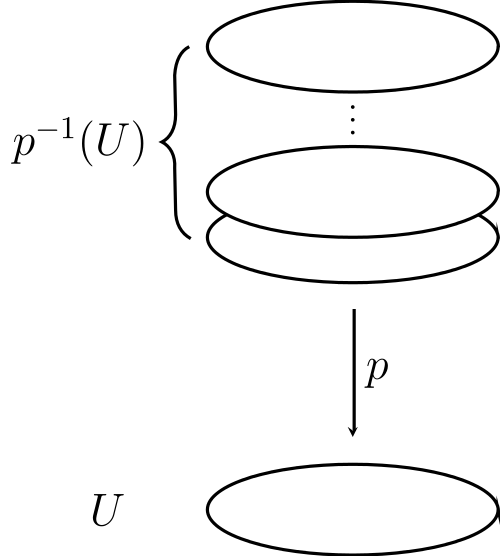
\includegraphics[width=4cm]{media/even-covering.png}
	\scriptsize Image from \cite{img:even_covering}
\end{center}
All we're saying is that $U$ is evenly covered if its pre-image
is a bunch of copies of it. (Actually, a little more: each of the pancakes is homeomorphic to $U$, but we also require that $p$ is the homeomorphism.)

\begin{definition}
	A \vocab{covering projection} $p : E \to B$
	is a continuous map such that every base point $b \in B$
	has a neighborhood $U \ni b$ which is evenly covered by $p$.
\end{definition}
\begin{ques}
	Why must a covering projection be surjective?
\end{ques}

Here is the most stupid example of a covering projection.
\begin{example}[Tautological covering projection]
	Let's take $n$ disconnected copies of any space $B$:
	formally, $E = B \times \{1, \dots, n\}$ with the discrete topology
	on $\{1, \dots, n\}$.
	Then there exists a tautological covering projection
	$E \to B$ by $(x,m) \mapsto x$;
	we just project all $n$ copies.

	This is a covering projection because \emph{every} open set in $B$
	is evenly covered.
\end{example}
This is not really that interesting because $B \times [n]$ is not path-connected.

A much more interesting example is that of $\RR$ and $S^1$.

\begin{example}[Covering projection of $S^1$]
	Take $p : \RR \to S^1$ by $\theta \mapsto e^{2\pi i \theta}$.
	This is essentially wrapping the real line
	into a single helix and projecting it down.
\end{example}
%\missingfigure{helix}

We claim this is a covering projection.
Indeed, consider the point $1 \in S^1$ (where we view $S^1$ as the unit circle in the complex plane). We can draw a small neighborhood of it
whose pre-image is a bunch of copies in $\RR$.
\begin{center}
	\begin{asy}
		size(12cm);

		real[] t = {-2,-1,0,1,2};
		xaxis(-3.5,3.5, graph.LeftTicks(Ticks=t), Arrows); 

		pen bloo = blue+1.5;

		dotfactor *= 2;
		pair A,B;
		for (real x = -2; x <= 2; ++x) {
			A = (x-0.2, 0); B = (x+0.2, 0);
			draw(A--B, bloo); opendot(A, blue); opendot(B, blue);
		}
		MP("\mathbb R", (3,0), dir(90));

		add(shift( (0,3) ) * CC());

		path darrow = (0,2.5)--(0,1.5);
		MP("p", midpoint(darrow), dir(0));
		draw(darrow, EndArrow);

		real r = 1.4;
		draw(scale(r)*unitcircle);
		MP("S^1", r*dir(45), dir(45));
		A = r*dir(-20);
		B = r*dir(20);
		draw(arc(origin, A, B), bloo);
		opendot(A, blue); opendot(B, blue);
		dot("$1$", r*dir(0), dir(0));
	\end{asy}
\end{center}

Note that not all neighborhoods work this time: notably, $U = S^1$ does not work because the pre-image would be the entire $\RR$.

\begin{example}[Covering of $S^1$ by itself]
	The map $S^1 \to S^1$ by
	$z \mapsto z^{3}$ is also a covering projection.
	Can you see why?
\end{example}

\begin{example}
	[Covering projections of $\CC \setminus \{0\}$]
	For those comfortable with complex arithmetic,
	\begin{enumerate}[(a)]
		\ii The exponential map $\exp : \CC \to \CC \setminus \{0\}$
		is a covering projection.
		\ii For each $n$, the $n$th power map
		$-^n: \CC \setminus \{0\} \to \CC \setminus \{0\}$
		is a covering projection.
	\end{enumerate}
\end{example}

\section{Lifting theorem}
\prototype{$\RR$ covers $S^1$.}
Now here's the key idea: we are going to try to interpret paths in $B$ as loops in $\RR$.
This is often much simpler.
For example, we had no idea how to compute the fundamental group of $S^1$,
but the fundamental group of $\RR$ is just the trivial group.
So if we can interpret loops in $S^1$ as loops in $\RR$, that might (and indeed it does!) make computing $\pi_1(S^1)$ tractable.

\begin{definition}
	Let $\gamma : [0,1] \to B$ be a path and $p : E \to B$ a covering projection.
	A \vocab{lifting} of $\gamma$ is a path $\tilde\gamma : [0,1] \to E$
	such that $p \circ \tilde\gamma = \gamma$.
\end{definition}
Picture:
\begin{diagram}
	&&& E \\
	&& \ruTo(3,2)^{\tilde \gamma} & \dTo_p \\
	[0,1] & \rTo^{\gamma} && b
\end{diagram}

\begin{example}[Typical example of lifting]
	Take $p : \RR \to S^1 \subseteq \CC$ by $\theta \mapsto e^{2 \pi i \theta}$
	(so $S^1$ is considered again as the unit circle).
	Consider the path $\gamma$ in $S^1$ which starts at $1 \in \CC$
	and wraps around $S^1$ once, counterclockwise, ending at $1$ again.
	In symbols, $\gamma : [0,1] \to S^1$ by $t \mapsto e^{2\pi i t}$.

	Then one lifting $\tilde\gamma$ is the path which walks from $0$ to $1$.
	In fact, \emph{for any integer $n$}, walking from $n$ to $n+1$ works.

	\begin{center}
		\begin{asy}
			size(6cm);

			real[] t = {-1,0,1,2};
			xaxis(-2,3, graph.LeftTicks(Ticks=t), Arrows); 
			MP("\mathbb R", (2.5,0), dir(90));
			path gt = (0,0.3)--(1,0.3);
			draw(gt, blue, EndArrow);
			label("$\tilde\gamma$", midpoint(gt), dir(90), blue);
			add(shift( (0,3) ) * CC());

			path darrow = (0,2.5)--(0,1.5);
			MP("p", midpoint(darrow), dir(0));
			draw(darrow, EndArrow);

			real r = 1.2;
			draw(scale(r)*unitcircle);
			MP("S^1", r*dir(45), dir(45));
			dot("$1$", r*dir(0), dir(0));
			path g = dir(20)..dir(100)..dir(180)..dir(260)..dir(340);
			draw(g, red, EndArrow);
			label("$\gamma$", midpoint(g), -dir(midpoint(g)), red);

			MP("p(0) = 1", (2.5,0.5));
			MP("p(1) = 1", (2.5,0));
		\end{asy}
	\end{center}

	Similarly, the counterclockwise path from $1 \in S^1$ to $-1 \in S^1$
	has a lifting: for some integer $n$, the path from $n$ to $n+\half$.
	\label{example:lifting_circle}
\end{example}

The above is the primary example of a lifting.
It seems like we have the following structure: given a path $\gamma$
in $B$ starting at $b_0$, we start at any point in the fiber $p\pre(b_0)$.
(In our prototypical example, $B = S^1$, $b_0 = 1 \in \CC$
and that's why we start at any integer $n$.)
After that we just trace along the path in $B$, and we get
a corresponding path in $E$.
\begin{ques}
	Take a path $\gamma$ in $S^1$ with $\gamma(0) = 1 \in \CC$.
	Convince yourself that once we select an integer $n \in \RR$,
	then there is exactly one lifting starting at $n$.
\end{ques}

It turns out this is true more generally.
\begin{theorem}[Lifting paths]
	Suppose $\gamma : [0,1] \to B$ is a path with $\gamma(0) = \gamma(1) = b_0$, and 
	$ p : (E,e_0) \to (B,b_0) $
	is a covering projection.
	Then there exists a \emph{unique} lifting $\tilde\gamma : [0,1] \to E$
	such that $\tilde\gamma(0) = e_0$.
\end{theorem}
\begin{proof}
	For every point $b \in B$, consider an evenly covered neighborhood $U_b$ in $B$.
	Then the family of open sets
	\[ \left\{ \gamma\pre(U_b) \mid b \in B \right\} \]
	is an open cover of $[0,1]$.
	As $[0,1]$ is compact we can take a finite subcover.
	Thus we can chop $[0,1]$ into finitely many disjoint closed intervals
	$[0,1] = I_1 \sqcup I_2 \sqcup \dots \sqcup I_N$ in that order,
	such that for every $I_k$, $\gamma``(I_k)$ is contained
	in some $U_b$.

	We'll construct $\tilde\gamma$ interval by interval now,
	starting at $I_1$.
	Initially, place a robot at $e_0 \in E$ and a mouse at $b_0 \in B$.
	For each interval $I_k$, the mouse moves around according
	to however $\gamma$ behaves on $I_k$.
	But the whole time it's in some evenly covered $U_k$;
	the fact that $p$ is a covering projection tells us that
	there are several copies of $U_k$ living in $E$.
	Exactly one of them, say $V_k$, contains our robot.
	So the robot just mimics the mouse until it gets to the end of $I_k$.
	Then the mouse is in some new evenly covered $U_{k+1}$,
	and we can repeat.
\end{proof}

The theorem can be generalized to a diagram
\begin{diagram}
	&& (E, e_0) \\
	& \ruTo^{\tilde f} & \dTo_{p} \\
	(Y,y_0) & \rTo^{f} & (B, b_0)
\end{diagram}
where $Y$ is some general path-connected space, as follows.
\begin{theorem}[General lifting criterion]
	\label{thm:lifting}
	Let $f: (Y,y_0) \to (B, b_0)$ be continuous and consider a covering projection $p : (E, e_0) \to (B, b_0)$.
	(As usual, $Y$, $B$, $E$ are path-connected.)
	Then a lifting $\tilde f$ with $\tilde f(y_0) = e_0$ exists if and only if
	\[ f_\ast``(\pi_1(Y, y_0)) \subseteq p_\ast``(\pi_1(E, e_0)), \]
	i.e.\ the image of $\pi_1(Y, y_0)$ under $f$ is contained in
	the image of $\pi_1(E, e_0)$ under $p$ (both viewed as subgroups of $\pi_1(B, b_0)$).
	If this lifting exists, it is unique.
\end{theorem}
As $p$ is injective, we actually have $p_\ast``(\pi_1(E, e_0)) \cong \pi_1(E, e_0)$.
But in this case we are interested in the actual elements, not just the isomorphism classes of the groups.
\begin{ques}
	What happens if we put $Y= [0,1]$?
\end{ques}

\begin{remark}[Lifting homotopies]
	Here's another cool special case:
	Recall that a homotopy can be encoded as a continuous function $[0,1] \times [0,1] \to X$.
	But $[0,1] \times [0,1]$ is also simply connected.
	Hence given a homotopy $\gamma_1 \simeq \gamma_2$ in the base space $B$, we can lift it to get
 a homotopy $\tilde\gamma_1 \simeq \tilde\gamma_2$ in $E$.
\end{remark}
Another nice application of this result is \Cref{ch:complex_log}.

\section{Lifting correspondence}
\prototype{$(\RR,0)$ covers $(S^1,1)$.}
Let's return to the task of computing fundamental groups.
Consider a covering projection $p : (E, e_0) \to (B, b_0)$.

A loop $\gamma$ can be lifted uniquely to $\tilde\gamma$ in $E$
which starts at $e_0$ and ends at some point $e$ in the fiber $p\pre(b_0)$.
You can easily check that this $e \in E$ does not change if we
pick a different path $\gamma'$ homotopic to $E$.
\begin{ques}
	Look at the picture in \Cref{example:lifting_circle}.

	Put one finger at $1 \in S^1$, and one finger on $0 \in \RR$.
	Trace a loop homotopic to $\gamma$ in $S^1$ (meaning, you can
	go backwards and forwards but you must end with exactly one full
	counterclockwise rotation)
	and follow along with the other finger in $\RR$.

	Convince yourself that you have to end at the point $1 \in \RR$.
\end{ques}

Thus every homotopy class of a loop at $b_0$ (i.e.\ an element of $\pi_1(B, b_0)$) can be associated with some $e$ in the fiber of $b_0$.
The below proposition summarizes this and more.
\begin{proposition}
	Let $p : (E,e_0) \to (B,b_0)$ be a covering projection.
	Then we have a function of sets
	\[ \Phi : \pi_1(B, b_0) \to p\pre(b_0) \]
	by $[\gamma] \mapsto \tilde\gamma(1)$, where $\tilde\gamma$
	is the unique lifting starting at $e_0$.
	Furthermore,
	\begin{itemize}
		\ii If $E$ is path-connected, then $\Phi$ is surjective.
		\ii If $E$ is simply connected, then $\Phi$ is injective.
	\end{itemize}
\end{proposition}
\begin{ques}
	Prove that $E$ path-connected implies $\Phi$ is surjective.
	(This is really offensively easy.)
\end{ques}
\begin{proof}
	To prove the proposition, we've done everything except show
	that $E$ simply connected implies $\Phi$ injective.
	To do this suppose that $\gamma_1$ and $\gamma_2$ are loops
	such that $\Phi([\gamma_1]) = \Phi([\gamma_2])$.

	Applying lifting, we get paths $\tilde\gamma_1$ and $\tilde\gamma_2$
	both starting at some point $e_0 \in E$ and ending at some point $e_1 \in E$.
	Since $E$ is simply connected that means they are \emph{homotopic},
	and we can write a homotopy $F : [0,1] \times [0,1] \to E$
	which unites them.
	But then consider the composition of maps
	\[ [0,1] \times [0,1] \taking{F} E \taking{p} B. \]
	You can check this is a homotopy from $\gamma_1$ to $\gamma_2$.
	Hence $[\gamma_1] \simeq [\gamma_2]$, done.
\end{proof}

This motivates:
\begin{definition}
	A \vocab{universal cover} of a space $B$ is a covering projection
	$p : E \to B$ where $E$ is simply connected (and in particular path-connected).
\end{definition}
\begin{abuse}
	When $p$ is understood, we sometimes just say $E$ is the universal cover.
\end{abuse}

\begin{example}[Fundamental group of $S^1$]
	Let's return to our standard $p : \RR \to S^1$.
	Since $\RR$ is simply connected, this is a universal cover of $S^1$.
	And indeed, the fiber of any point in $S^1$
	is a copy of the integers: naturally in bijection with loops in $S^1$.
	
	You can show (and it's intuitively obvious) that the bijection
	\[ \Phi : \pi_1(S^1) \leftrightarrow \ZZ \]
	is in fact a group homomorphism if we equip $\ZZ$ with its
	additive group structure $\ZZ$.
	Since it's a bijection, this leads us to conclude $\pi_1(S^1) \cong \ZZ$.
\end{example}

\section{Regular coverings}
I want to talk a little about a special type of covering now: those
that arise from group actions.

Let $X$ be a topological space and $G$ a group acting on its points.
Thus for every $g$, we get a map $X \to X$ by 
\[ x \mapsto g \cdot x. \]
We require that this map is continuous for every $g \in G$.\footnote{%
	Another way of phrasing this: the action,
	interpreted as a map $X \times G \to X$, should be continuous,
	where $G$ on the left-hand side is interpreted as a set with
	the discrete topology.}

Then we can consider a topological space $X/G$ defined by fusing any points
in the same orbit of this action.
(The open sets of $X/G$ are just the open sets of $X$ after this identification.)
In other words, the points of $X/G$ are the orbits of the action.
Then we get a natural ``projection''
\[ X \to X/G \]
by simply sending every point to the orbit it lives in.
\begin{definition}
	Such a projection is called \vocab{regular}.
	(Terrible, I know.)
\end{definition}

\begin{example}[$\RR \to S^1$ is regular]
	Let $G = \ZZ$, $X = \RR$
	and define the group action of $G$ on $X$ by 
	\[ n \cdot x = n + x \]
	You can then think of $X/G$ as ``real numbers modulo $1$'',
	with $[0,1)$ a complete set of representatives and $0 \sim 1$.
	\begin{center}
		\begin{asy}
			size(9cm);
			dotfactor *= 2;
			pair A = MP("0", (-5.1,0), 1.4*dir(90));
			pair B = MP("1", (-3,0), 1.4*dir(90));
			draw(A--B);
			D("\frac13", (-4.4,0), 1.4*dir(90));
			D("\frac23", (-3.7,0), 1.4*dir(90));
			MP("\mathbb R / G", (-4,-0.6), dir(-90));
			dot(A); opendot(B);
			draw(unitcircle);
			draw( (-2.4,0)--(-1.6,0), EndArrow);
			dot("$0=1$", dir(0), dir(0));
			dot("$\frac13$", dir(120), dir(120));
			dot("$\frac23$", dir(240), dir(240));
			label("$S^1$", origin, origin);
		\end{asy}
	\end{center}
	So we can identify $X/G$ with $S^1$
	and the associated regular projection
	is just our usual $\exp : \theta \mapsto e^{2i\pi \theta}$.
\end{example}
	
\begin{example}[The torus]
	Let $G = \ZZ \times \ZZ$ and $X = \RR^2$,
	and define the group action of $G$ on $X$ by $(m,n) \cdot (x,y)
	= (m+x, n+y)$.
	As $[0,1)^2$ is a complete set of representatives,
	you can think of it as a unit square with the edges identified.
	We obtain the torus $S^1 \times S^1$
	and a covering projection $\RR^2 \to S^1 \times S^1$.
\end{example}

\begin{example}[$\mathbb {RP}^2$]
	Let $G = \Zc 2 = \left<T \mid T^2 = 1\right>$ and
	let $X = S^2$ be the surface of the sphere,
	viewed as a subset of $\RR^3$.
	We'll let $G$ act on $X$ by sending $T \cdot \vec x = - \vec x$;
	hence the orbits are pairs of opposite points (e.g.\ North and South pole).

	Let's draw a picture of a space.
	All the orbits have size two:
	every point below the equator gets fused with a point above the equator.
	As for the points on the equator, we can take half of them; the other half
	gets fused with the corresponding antipodes.

	Now if we flatten everything,
	you can think of the result as a disk with half its boundary:
	this is $\RP^2$ from before.
	The resulting space has a name: \emph{real projective $2$-space},
	denoted $\mathbb{RP}^2$.
	\begin{center}
		\begin{asy}
			size(3cm);
			dotfactor *= 2;
			draw(dir(-90)..dir(0)..dir(90));
			draw(dir(90)..dir(180)..dir(-90), dashed);
			fill(unitcircle, yellow+opacity(0.2));
			dot(dir(90));
			opendot(dir(-90));
			label("$\mathbb{RP}^2$", origin, origin);
		\end{asy}
	\end{center}

	This gives us a covering projection $S^2 \to \mathbb{RP}^2$
	(note that the pre-image of a sufficiently small patch is just two copies
	of it on $S^2$.)
\end{example}
\begin{example}
	[Fundamental group of $\mathbb{RP}^2$]
	As above, we saw that there was a covering projection
	$S^2 \to \mathbb{RP}^2$.
	Moreover the fiber of any point has size two.
	Since $S^2$ is simply connected, we have a natural bijection
	$\pi_1(\mathbb{RP}^2)$ to a set of size two; that is,
	\[ \left\lvert \pi_1(\mathbb{RP}^2) \right\rvert = 2. \]
	This can only occur if $\pi_1(\mathbb{RP}^2) \cong \Zc 2$,
	as there is only one group of order two!
\end{example}

\begin{ques}
	Show each of the continuous maps $x \mapsto g \cdot x$ is in fact a homeomorphism.
	(Name its continuous inverse).
\end{ques}
% WOW I thought this was always a covering projection gg

\section{The algebra of fundamental groups}
\prototype{$S^1$, with fundamental group $\ZZ$.}
Next up, we're going to turn functions between spaces into homomorphisms of fundamental groups.

Let $X$ and $Y$ be topological spaces and $f : (X, x_0) \to (Y, y_0)$.
Recall that we defined a group homomorphism
\[ f_\sharp : \pi_1(X, x_0) \to \pi_1(Y_0, y_0) 
	\quad\text{by}\quad
	[\gamma] \mapsto [f \circ \gamma]. \]
% which gave us a functor $\catname{Top}_\ast \to \catname{Grp}$.

More importantly, we have:
\begin{proposition}
	Let $p : (E,e_0) \to (B,b_0)$ be a covering projection of path-connected spaces.
	Then the homomorphism $p_\sharp : \pi_1(E, e_0) \to \pi_1(B, b_0)$ is \emph{injective}.
	Hence $p_\sharp ``(\pi_1(E, e_0))$ is an isomorphic copy of $\pi_1(E, e_0)$ 
	as a subgroup of $\pi_1(B, b_0)$.
\end{proposition}
\begin{proof}
	We'll show $\ker p_\sharp$ is trivial.
	It suffices to show if $\gamma$ is a nulhomotopic loop in $B$ 
	then its lift is nulhomotopic.

	By definition, there's a homotopy $F : [0,1] \times [0,1] \to B$
	taking $\gamma$ to the constant loop $1_B$.
	We can lift it to a homotopy $\tilde F : [0,1] \times [0,1] \to E$
	that establishes $\tilde\gamma \simeq \tilde 1_B$.
	But $1_E$ is a lift of $1_B$ (duh) and lifts are unique.
\end{proof}

\begin{example}[Subgroups of $\ZZ$]
	Let's look at the space $S^1$ with fundamental group $\ZZ$.
	The group $\ZZ$ has two types of subgroups:
	\begin{itemize}
		\ii The trivial subgroup.
		This corresponds to the canonical projection $\RR \to S^1$,
		since $\pi_1(\RR)$ is the trivial group ($\RR$ is simply connected)
		and hence its image in $\ZZ$ is the trivial group.
		\ii $n\ZZ$ for $n \ge 1$.
		This is given by the covering projection $S^1 \to S^1$
		by $z \mapsto z^n$.
		The image of a loop in the covering $S^1$ is a ``multiple of $n$''
		in the base $S^1$.
	\end{itemize}
\end{example}

It turns out that these are the \emph{only} covering projections of $S^n$ by path-connected spaces: there's one for each subgroup of $\ZZ$.
(We don't care about disconnected spaces because, again, a covering projection
via disconnected spaces is just a bunch of unrelated ``good'' coverings.)
For this statement to make sense I need to tell you what it means for
two covering projections to be equivalent.

\begin{definition}
	Fix a space $B$.
	Given two covering projections $p_1 : E_1 \to B$ and $p_2 : E_2 \to B$
	a \vocab{map of covering projections} is a continuous function $f : E_1 \to E_2$
	such that $p_2 \circ f = p_1$.
	\begin{diagram}
		E_1 & \rTo^f && E_2 \\
		& \rdTo(3,2)_{p_1} && \dTo_{p_2} \\
		&&& B
	\end{diagram}
	Then two covering projections $p_1$ and $p_2$ are isomorphic if there are
	$f : E_1 \to E_2$ and $g : E_2 \to E_1$
	such that $f \circ g = \id_{E_1}$ and $g \circ f = \id_{E_2}$.
\end{definition}
\begin{remark}
	[For category theorists]
	The set of covering projections forms a category in this way.
\end{remark}

It's an absolute miracle that this is true more generally:
the greatest triumph of covering spaces is the following result.
Suppose a space $X$ satisfies some nice conditions, like:
\begin{definition}
	A space $X$ is called \vocab{locally connected} if each point $x \in X$
	has a connected neighborhood $U$.
\end{definition}
\begin{definition}
	A space $X$ is \vocab{semi-locally simply connected} if for every point $x \in X$
	there is a neighborhood $U$ such that all loops in $U$ are nulhomotopic.
	(But the contraction need not take place in $U$.)
\end{definition}
\begin{example}[These conditions are weak]
	Pretty much every space I've shown you has these two properties.
	In other words, they are rather mild conditions, and you can think of them as just
	saying ``the space is not too pathological''.
\end{example}
Then we get:
\begin{theorem}[Group theory via covering spaces]
	Suppose $B$ is a connected, locally connected, semi-locally simply connected space.
	Then:
	\begin{itemize}
		\ii Every subgroup $H \subseteq \pi_1(B)$ corresponds
		to exactly one covering projection $p : E \to B$
		with $E$ path-connected (up to isomorphism).

		(Specifically, $H$ is the image of $\pi_1(E)$ in $\pi_1(B)$ through $p_\sharp$.)
		\ii Moreover, the \emph{normal} subgroups of $\pi_1(B)$
		correspond exactly to the regular covering projections.
	\end{itemize}
\end{theorem}
Hence it's possible to understand the group theory of $\pi_1(B)$ completely
in terms of the covering projections.

Moreover, this is how the ``universal cover'' gets its name:
it is the one corresponding to the trivial subgroup of $\pi_1(B)$.
Actually, you can show that it really is universal in the sense
that if $p : E \to B$ is another covering projection,
then $E$ is in turn covered by the universal space.
More generally, if $H_1 \subseteq H_2 \subseteq G$ are subgroups,
then the space corresponding to $H_2$ can be covered by the space
corresponding to $H_1$.

% According to \cite{ref:covering_all_we_know}, this statement and
% its extension to group actions are ``pretty much all there is to know
% about covering projections''.

\section\problemhead
%% TODO problems
 % missing problems

\part{Category Theory}
\chapter{Objects and morphisms}
\label{ch:cats}
I can't possibly hope to do category theory any justice in these few chapters;
thus I'll just give a very high-level overview of how many of the concepts we've
encountered so far can be re-cast into categorical terms.
So I'll say what a category is, give some examples,
then talk about a few things that categories can do.
For my examples, I'll be drawing from all the previous chapters;
feel free to skip over the examples corresponding to things you haven't seen.

If you're interested in category theory (like I was!), perhaps in
what surprising results are true for general categories, I strongly recommend \cite{ref:msci}.

\section{Motivation: isomorphisms}
From earlier chapters let's recall the definition of an \emph{isomorphism} of two objects:
\begin{itemize}
	\ii Two groups $G$ and $H$ are isomorphic if there was a bijective homomorphism:
	equivalently, we wanted homomorphisms $\phi : G \to H$ and $\psi : H \to G$
	which were mutual inverses, meaning $\phi \circ \psi = \id_H$ and $\psi \circ \phi = \id_G$.
	\ii Two metric (or topological) spaces $X$ and $Y$ are isomorphic
	if there is a continuous bijection $f : X \to Y$ such that $f\inv$ is also continuous.
	\ii Two vector spaces $V$ and $W$ are isomorphic if there is a bijection $T : V \to W$
	which is a linear map.
	Again, this can be re-cast as saying that $T$ and $T\inv$ are continuous maps.
	\ii Two rings $R$ and $S$ are isomorphic if there is a bijective ring homomorphism $\phi$;
	again, we can re-cast this as two mutually inverse ring homomorphisms.
\end{itemize}

In each case we have some collections of objects and some maps,
and the isomorphisms can be viewed as just maps.
Let's use this to motivate the definition of a general \emph{category}.

\section{Categories, and examples thereof}
\prototype{$\catname{Grp}$ is possibly the most natural example.}
\begin{definition}
	A \vocab{category} $\AA$ consists of:
	\begin{itemize}
		\ii A class of \vocab{objects}, denoted $\obj(\AA)$.
		\ii For any two objects $A_1, A_2 \in \obj(\AA)$, 
		a class of \vocab{arrows} (also called \vocab{morphisms} or \vocab{maps}) between them.
		We'll denote the set of these arrows by $\Hom_\AA(A_1, A_2)$.
		\ii For any $A_1, A_2, A_3 \in \obj(\AA)$,
		if $f : A_1 \to A_2$ is an arrow and $g : A_2 \to A_3$ is an arrow, we can compose
		these arrows to get an arrow $g \circ f : A_1 \to A_3$.

		We can represent this in a \vocab{commutative diagram}
		\begin{diagram}
			A_1 & \rTo^f & A_2 \\
			& \rdDashed^h & \dTo_g \\
			&& A_3
		\end{diagram}
		where $h = g \circ f$.
		The composition operation $\circ$ is part of the data of $\AA$;
		it must be associative.
		In the diagram above we say that $h$ \vocab{factors} through $A_2$.
		
		\ii Finally, every object $A \in \obj(\AA)$ has a special \vocab{identity arrow} $\id_A$;
		you can guess what it does.\footnote{To be painfully explicit: if $f : A' \to A$ is an arrow then $\id_A \circ f = f$;
		similarly, if $g : A \to A'$ is an arrow then $g \circ \id_A = g$.}
	\end{itemize}
\end{definition}
\begin{abuse}
	From now on, by $A \in \AA$ we'll mean $A \in \obj(\AA)$.
\end{abuse}
\begin{abuse}
	You can think of ``class'' as just ``set''.
	The reason we can't use the word ``set'' is
	because of some paradoxical issues with
	collections which are too large;
	Cantor's Paradox says there is no set of all sets.
	So referring to these by ``class'' is a way of sidestepping these issues.

	Now and forever I'll be sloppy and assume all my categories
	are \vocab{locally small}, meaning that $\Hom_{\AA} (A_1, A_2)$
	is a set for any $A_1, A_2 \in \AA$.
	So elements of $\AA$ may not form a set,
	but the set of morphisms between
	two \emph{given} objects will always assumed to be a set.
\end{abuse}

Let's formalize the motivation we began with.
\begin{example}
	[Basic examples of categories]
	\listhack
	\label{example:basic_categories}
	\begin{enumerate}[(a)]
		\ii There is a category of groups $\catname{Grp}$. The data is
		\begin{itemize}
			\ii The objects of $\catname{Grp}$ are the groups.
			\ii The arrows of $\catname{Grp}$ are the homomorphisms between these groups.
			\ii The composition $\circ$ in $\catname{Grp}$ is function composition.
		\end{itemize}
		\ii In the same way we can conceive a category $\catname{CRing}$ of (commutative) rings.
		\ii Similarly, there is a category $\catname{Top}$ of topological spaces,
		whose arrows are the continuous maps.
		\ii There is a category $\catname{Top}_\ast$ of topological spaces with a \emph{distinguished basepoint};
		that is, a pair $(X, x_0)$ where $x_0 \in X$.
		Arrows are continuous maps $f : X \to Y$ with $f(x_0) = y_0$.
		\ii Similarly, there is a category $\catname{Vect}_k$ of
		vector spaces (possibly infinite-dimensional) over a field $k$,
		whose arrows are the linear maps.
		There is even a category $\catname{FDVect}_k$ of
		\emph{finite-dimensional} vector spaces.
		\ii We have a category $\catname{Set}$ of sets,
		where the arrows are \emph{any} maps.
	\end{enumerate}
\end{example}
And of course, we can now define what an isomorphism is!
\begin{definition}
	An arrow $A_1 \taking{f} A_2$ is an \vocab{isomorphism}
	if there exists $A_2 \taking{g} A_1$ such that $f \circ g = \id_{A_2}$
	and $g \circ f = \id_{A_1}$.
	In that case we say $A_1$ and $A_2$ are \vocab{isomorphic}, hence $A_1 \cong A_2$.
\end{definition}
\begin{remark}
	Note that in $\catname{Set}$, $X \cong Y
	\iff \left\lvert X \right\rvert = \left\lvert Y \right\rvert$.
\end{remark}
\begin{ques}
	Check that every object in a category is isomorphic to itself.
	(This is offensively easy.)
\end{ques}
More importantly, this definition should strike you as a little impressive.
We're able to define whether two groups (rings, spaces, etc.) are isomorphic
solely by the functions between the objects.
Indeed, one of the key themes in category theory (and even algebra) is that
\begin{moral}
	One can learn about objects by the functions between them.
	Category theory takes this to the extreme by \emph{only} looking at arrows,
	and ignoring what the objects themselves are.
\end{moral}

But there are some trickier interesting examples of categories.
\begin{example}
	[Posets are categories]
	Let $\mathcal P$ be a partially ordered set.
	We can construct a category $P$ for it as follows:
	\begin{itemize}
		\ii The objects of $P$ are going to be the elements of $\mathcal P$.
		\ii The arrows of $P$ are defined as follows:
		\begin{itemize}
			\ii For every object $p \in P$, we add an identity arrow $\id_p$, and
			\ii For any pair of distinct objects $p \le q$, we add a single arrow $p \to q$.
		\end{itemize}
		There are no other arrows.
		\ii There's only one way to do the composition. What is it?
	\end{itemize}
\end{example}
For example, for the poset $\mathcal P$ on four objects $\{a,b,c,d\}$ with $a \le b$ and $a \le c \le d$, we get:
\begin{center}
\begin{tikzpicture}[scale=3.5]
	\SetVertexMath
	\Vertices{square}{d,c,a,b}
	\Edge[style={->}, label={$a \le b$}](a)(b)
	\Edge[style={->}, label={$a \le c$}](a)(c)
	\Edge[style={->}, label={$a \le d$}](a)(d)
	\Edge[style={->}, label={$c \le d$}](c)(d)
	\Loop[dist=8, dir=NO, label={$\id_a$}, labelstyle={above=1pt}](a)
	\Loop[dist=8, dir=WE, label={$\id_b$}, labelstyle={left=1pt}](b)
	\Loop[dist=8, dir=EA, label={$\id_c$}, labelstyle={right=1pt}](c)
	\Loop[dist=8, dir=WE, label={$\id_d$}, labelstyle={left=1pt}](d)
\end{tikzpicture}
\end{center}

This illustrates the point that
\begin{moral}
	The arrows of a category can be totally different from functions.
\end{moral}
In fact, in a way that can be made precise, the term ``concrete category'' refers
to one where the arrows really are ``structure-preserving maps between sets'',
like $\catname{Grp}$, $\catname{Top}$, or $\catname{CRing}$.

\begin{ques}
	Check that no two distinct objects of a poset are isomorphic.
\end{ques}

Here's a second quite important example of a non-concrete category.
\begin{example}
	[Important: groups are one-Object categories]
	A group $G$ can be interpreted as a category $\mathcal G$ with one object $\ast$,
	all of whose arrows are isomorphisms.

	\begin{center}
	\begin{tikzpicture}[scale=5.5]
		\Vertex[x=0,y=0,L={$\ast$}]{a}
		\Loop[dist=8, dir=NO, label={$1 = \id_a$}, labelstyle={above=1pt}](a)
		\Loop[dist=7, dir=WE, label={$g_2$}, labelstyle={left=1pt}](a)
		\Loop[dist=9, dir=SO, label={$g_3$}, labelstyle={below=1pt}](a)
		\Loop[dist=8, dir=EA, label={$g_4$}, labelstyle={right=1pt}](a)
	\end{tikzpicture}
	\end{center}

	As \cite{ref:msci} says:

	\begin{quote}
	The first time you meet the idea that a group is a kind of category,
	it's tempting to dismiss it as a coincidence or a trick.
	It's not: there's real content.
	To see this, suppose your education had been shuffled and you took a course
	on category theory before ever learning what a group was.
	Someone comes to you and says: 

	``There are these structures called `groups', and the idea is this:
	a group is what you get when you collect together all the symmetries
	of a given thing.''

	``What do you mean by a `symmetry'?'' you ask.

	``Well, a symmetry of an object $X$ is a way of transforming $X$ or mapping
	$X$ into itself, in an invertible way.''

	``Oh,'' you reply, ``that's a special case of an idea I've met before.
	A category is the structure formed by \emph{lots} of objects and mappings
	between them -- not necessarily invertible. A group's just the very special case
	where you've only got one object, and all the maps happen to be invertible.''
	\end{quote}
\end{example}

\begin{exercise}
	Verify the above!
	That is, show that the data of a one-object category with all isomorphisms
	is the same as the data of a group.
\end{exercise}

Finally, here are some examples of categories you can make from other categories.
\begin{example}
	[Deriving categories]
	\listhack
	\begin{enumerate}[(a)]
		\ii Given a category $\AA$, we can construct the \vocab{opposite category}
		$\AA\op$, which is the same as $\AA$ but with all arrows reversed.
		\ii Given categories $\AA$ and $\BB$, we can construct the \vocab{product category} $\AA \times \BB$
		as follows: the objects are pairs $(A, B)$ for $A \in \AA$ and $B \in \BB$,
		and the arrows from $(A_1, B_1)$ to $(A_2, B_2)$
		are pairs \[ \left( A_1 \taking{f} A_2, B_1 \taking{g} B_2 \right). \]
		What do you think the composition and identities are?
	\end{enumerate}
\end{example}

\section{Special objects in categories}
\prototype{$\catname{Set}$ has initial object $\varnothing$ and final object $\{\ast\}$. An element of $S$ corresponds to a map $\{\ast\} \to S$.}
Certain objects in categories have special properties.
Here are a couple examples.
\begin{example}
	[Initial object]
	An \vocab{initial object} of $\AA$ is an object
	$A_{\text{init}} \in \AA$ such that for any $A \in \AA$ (possibly $A = A_{\text{init}}$),
	there is exactly one arrow from $A_{\text{init}}$ to $A$.
	For example,
	\begin{enumerate}[(a)]
		\ii The initial object of $\catname{Set}$ is the empty set $\varnothing$.
		\ii The initial object of $\catname{Grp}$ is the trivial group $\{1\}$.
		\ii The initial object of $\catname{CRing}$ is the ring $\ZZ$
		(recall that ring homomorphisms $R \to S$ map $1_R$ to $1_S$).
		\ii The initial object of $\catname{Top}$ is the empty space.
		\ii The initial object of a partially ordered set is its smallest element, if one exists.
	\end{enumerate}
\end{example}

We will usually refer to ``the'' initial object of a category, since:
\begin{exercise}
	[Important!]
	Show that any two initial objects $A_1$, $A_2$ of $\AA$ are \emph{uniquely isomorphic}
	meaning there is a unique isomorphism between them.
\end{exercise}

\begin{remark}
	In mathematics, we usually neither know nor care if two objects are actually equal
	or whether they are isomorphic.
	For example, there are many competing ways to define $\RR$,
	but we still just refer to it as ``the'' real numbers.

	Thus when we define categorical notions, we would like to check they are
	unique up to isomorphism.
	This is really clean in the language of categories, and definitions
	often cause objects to be unique up to isomorphism for elegant reasons like the above.
\end{remark}

One can take the ``dual'' notion, a terminal object.
\begin{example}
	[Terminal object]
	A \vocab{terminal object} of $\AA$ is an object
	$A_{\text{final}} \in \AA$ such that for any $A \in \AA$ (possibly $A = A_{\text{final}}$),
	there is exactly one arrow from $A$ to $A_{\text{final}}$.
	For example,
	\begin{enumerate}[(a)]
		\ii The terminal object of $\catname{Set}$ is the singleton set $\{\ast\}$.
		(There are many singleton sets, of course, but \emph{as sets} they are all isomorphic!)
		\ii The terminal object of $\catname{Grp}$ is the trivial group $\{1\}$.
		\ii The terminal object of $\catname{CRing}$ is the zero ring (a ring with element $0=1$).
		(Recall that ring homomorphisms $R \to S$ must map $1_R$ to $1_S$).
		\ii The terminal object of $\catname{Top}$ is the single-point space.
		\ii The terminal object of a partially ordered set is its maximal element, if one exists.
	\end{enumerate}
\end{example}

Again, terminal objects are unique up to isomorphism.
The reader is invited to repeat the proof from the preceding exercise here.
However, we can illustrate more strongly the notion of duality to give a short proof.
\begin{ques}
	Verify that terminal objects of $\AA$ are equivalent to initial objects of $\AA\op$.
	Thus terminal objects of $\AA$ are unique up to isomorphism.
\end{ques}
In general, one can consider in this way the dual of \emph{any} categorical notion:
properties of $\AA$ can all be translated to dual properties of $\AA\op$
(often by adding the prefix ``co'' in front).

One last neat construction: suppose we're working in a concrete category,
meaning (loosely) that the objects are ``sets with additional structure''.
Now suppose you're sick of maps and just want to think about elements of these sets.
Well, I won't let you do that since you're reading a category theory chapter,
but I will offer you some advice:
\begin{itemize}
	\ii In $\catname{Set}$, arrows from $\{\ast\}$ to $S$ correspond to elements of $S$.
	\ii In $\catname{Top}$, arrows from $\{\ast\}$ to $X$ correspond to points of $X$.
	\ii In $\catname{Grp}$, arrows from $\ZZ$ to $G$ correspond to elements of $G$.
	\ii In $\catname{CRing}$, arrows from $\ZZ[x]$ to $R$ correspond to elements of $R$.
\end{itemize}
and so on.
So in most concrete categories, you can think of elements as functions from special sets to the set in question.
In each of these cases we call the object in question a \vocab{free object}.

\section{Binary products}
\prototype{$X \times Y$ in most concrete categories is the set-theoretic product.}
The ``universal property'' is a way of describing objects in terms of maps
in such a way that it defines the object up to unique isomorphism
(much the same as the initial and terminal objects).

To show how this works in general, let me give a concrete example.
Suppose I'm in a category -- let's say $\catname{Set}$ for now.
I have two sets $X$ and $Y$, and I want to construct the Cartesian product $X \times Y$ as we know it.
The philosophy of category theory dictates that I should talk about maps only,
and avoid referring to anything about the sets themselves.
How might I do this?

Well, let's think about maps into $X \times Y$.
The key observation is that 
\begin{moral}
A function $A \taking f X \times Y$
amounts to a pair of functions $(A \taking g X, A \taking h Y)$.
\end{moral}
Put another way, there is a natural projection map $X \times Y \surjto X$ and $X \times Y \surjto Y$:
\begin{diagram}
	&& X \\
	X \times Y & \ruSurj(2,1)^{\pi_X} & \\
	& \rdSurj(2,1)_{\pi_Y} & Y
\end{diagram}
(We have to do this in terms of projection maps rather than elements,
because category theory forces us to talk about arrows.)
Now how do I add $A$ to this diagram?
The point is that there is a bijection between functions $A \taking f X \times Y$
and pairs $(g,h)$ of functions.
Thus for every pair $A \taking g X$ and $A \taking h Y$ there is a \emph{unique} function
$A \taking f X \times Y$.

But $X \times Y$ is special in that it is ``universal'':
for any \emph{other} set $A$, if you give me functions $A \to X$ and $A \to Y$, I can use it
build a \emph{unique} function $A \to X \times Y$.
Picture:
\begin{diagram}
	&& && X \\
	A & \rDotted~{\exists! f} & X \times Y & \ruTo(4,1)^g \ruSurj(2,1)_{\pi_X} & \\
	& \rdTo(4,1)_h && \rdProj(2,1)^{\pi_Y} & Y
\end{diagram}
We can do this in any general category, defining a so-called product.
\begin{definition}
	Let $X$ and $Y$ be objects in any category $\AA$.
	The \vocab{product} consists of an object $X \times Y$
	and arrows $\pi_X$, $\pi_Y$ to $X$ and $Y$ (thought of as projection).
	We require that for any object $A$ and arrows $A \taking g X$, $A \taking h Y$, there
	is a \emph{unique} function $A \taking f X \times Y$ such that the diagram
	\begin{diagram}
		&& && X \\
		A & \rDotted~{\exists! f} & X \times Y & \ruTo(4,1)^g \ruProj(2,1)_{\pi_X} & \\
		& \rdTo(4,1)_h && \rdProj(2,1)^{\pi_Y} & Y
	\end{diagram}
	commutes.
\end{definition}
\begin{abuse}
	Strictly speaking, the product should consist of \emph{both}
	the object $X \times Y$
	and the projection maps $\pi_X$ and $\pi_Y$.
	However, if $\pi_X$ and $\pi_Y$ are understood,
	then we often use $X \times Y$ to refer to the object,
	and refer to it also as the product.
	\label{abuse:object}
\end{abuse}

Products do not always exist; for example,
take a category with just two objects and no non-identity morphisms.
Nonetheless:
\begin{proposition}[Uniqueness of products]
	When they exist, products are unique up to isomorphism:
	given two products $P_1$ and $P_2$ of $X$ and $Y$
	there is an isomorphism between the two objects.
\end{proposition}
\begin{proof}
	This is very similar to the proof that initial objects are unique up to unique isomorphism.
	Consider two such objects $P_1$ and $P_2$, and the associated projection maps.
	So, we have a diagram
	\begin{diagram}
		&& X && \\
		& \ruProj^{\pi_X^1} & \uProj_{\pi_X^2} & \luProj^{\pi_X^1} & \\
		P_1 & \rTo~f & P_2 & \rTo~g & P_1 \\
		& \rdProj_{\pi_Y^1} & \dProj_{\pi_Y^2} & \ldProj_{\pi_Y^1} & \\
		&& Y &&
	\end{diagram}
	There are unique morphisms $f$ and $g$ between $P_1$ and $P_2$ that
	make the entire diagram commute, according to the universal property.

	On the other hand, look at $g \circ f$ and focus on just the outer square.
	Observe that $g \circ f$ is a map which makes the outer square commute,
	so by the universal property of $P_1$ it is the only one.
	But $\id_{P_1}$ works as well.
	Thus $\id_{P_1} = g \circ f$.
	Similarly, $f \circ g = \id_{P_2}$ so $f$ and $g$ are isomorphisms.
\end{proof}
\begin{abuse}
	Actually, this is not really the morally correct theorem;
	since we've only showed the objects $P_1$ and $P_2$ are isomorphic
	and have not made any assertion about the projection maps.
	But I haven't (and won't) define isomorphism of the entire product,
	and so in what follows if I say ``$P_1$ and $P_2$ are isomorphic''
	I really just mean the objects are isomorphic.
\end{abuse}
\begin{exercise}
	In fact, show the products are unique up to \emph{unique} isomorphism:
	the $f$ and $g$ above are the only isomorphisms between
	the objects $P_1$ and $P_2$.
\end{exercise}

The nice fact about this ``universal property'' mindset
is that we don't have to give explicit constructions; assuming existence,
the ``universal property'' allows us to bypass all this work by saying
``the object with these properties is unique up to unique isomorphism'',
thus we don't need to understand the internal workings of the object
to use its properties.

Of course, that's not to say we can't give concrete examples.
\begin{example}
	[Examples of products]
	\listhack
	\begin{enumerate}[(a)]
		\ii In $\catname{Set}$, the product of two sets $X$ and $Y$ is their Cartesian product.
		\ii In $\catname{Grp}$, the product of $G$, $H$ is the group product $G \times H$.
		\ii In $\catname{Vect}_k$, the product of $V$ and $W$ is $V \oplus W$.
		\ii Let $\mathcal P$ be a poset interpreted as a product.
		Then the product of two objects $x$ and $y$ is the \vocab{greatest lower bound};
		for example,
		\begin{itemize}
			\ii If the poset is $(\RR, \le)$ then it's $\min\{x,y\}$.
			\ii If the poset is the subsets of a finite set by inclusion, then it's $x \cap y$.
			\ii If the poset is the positive integers ordered by division, then it's $\gcd(x,y)$.
		\end{itemize}
	\end{enumerate}
\end{example}

Of course, we can define products of more than just one object.
Consider a set of objects $(X_i)_{i \in I}$ in a category $\AA$.
We define a \vocab{cone} on the $X_i$ to be an object $A$
with some ``projection'' maps to each $X_i$.
Then the \vocab{product} is a cone $P$ which is ``universal'' in the same sense as before:
given any other cone $A$ there is a unique map $A \to P$ making the diagram commute.
In short, a product is a ``universal cone''.

The picture of this is
\begin{diagram}
	&& A && \\
	& \ldProj(2,4) \ldProj(1,4) & \dTo~{!\exists f} & \rdProj(2,4) \rdProj(1,4)& \\
	&& P && \\
	& \ldProj \ldProj(1,2) && \rdProj \rdProj(1,2) & \\
	X_1 & X_2 && X_3 & X_4
\end{diagram}
See also \Cref{prob:associative_product}.

One can also do the dual construction to get a \vocab{coproduct}:
given $X$ and $Y$, it's the object $X+Y$
together with maps $X \taking{\iota_X} X+Y$ and $Y \taking{\iota_Y} X+Y$
(that's Greek iota, think inclusion)
such that for any object $A$ and maps $X \taking g A$, $Y \taking h A$
there is a unique $f$ for which
\begin{diagram}
	X &&&& \\
	& \rdTo(1,2)_{\iota_X} \rdTo(3,2)^g && \\
	& X+Y & \rTo~{!\exists f} & A \\
	\ruTo(1,2)^{\iota^Y} && \ruTo(3,2)_h & \\
	Y &&&&
\end{diagram}
commutes.
We'll leave some of the concrete examples as an exercise this time,
for example:
\begin{exercise}
	Describe the coproduct in $\catname{Set}$.
\end{exercise}
Predictable terminology: a coproduct is a universal \vocab{cocone}.

\section{Equalizers}
\prototype{The equalizer of $f,g : X \to Y$ is the set of points with $f(x) = g(x)$.}
Given two sets $X$ and $Y$, and maps $X \taking{f,g} Y$, we define their \vocab{equalizer} to be
\[ \left\{ x \in X \mid f(x) = g(x) \right\}. \]
We would like a categorical way of defining this, too.

Consider two objects $X$ and $Y$ with two maps $f$ and $g$ between them.
Stealing a page from \cite{ref:msci}, we call this a \vocab{fork}:
\begin{diagram}
	X & \pile{\rTo^f \\ \rTo_g} & Y
\end{diagram}
A cone over this fork is an object $A$ and arrows over $X$ and $Y$ which make the diagram commute, like so.
\begin{diagram}
	A && \\
	\dTo^q & \rdDashed^{f \circ q = g \circ q} & \\
	X & \pile{\rTo^f \\ \rTo_g} & Y
\end{diagram}
Effectively, the arrow over $Y$ is just forcing $f \circ q = g \circ q$.
In any case, the \vocab{equalizer} of $f$ and $g$ is a ``universal cone'' over this fork:
it is an object $E$ and a map $E \taking{e} X$ such that
for each $A \taking q X$ the diagram
\begin{diagram}
	& A & \\
	\ldTo(1,3)^q & \dTo~{!\exists h} & \rdDashed(1,3) \\
	& E & \\
	X \ldTo(1,1)^e & \pile{\rTo^f \\ \rTo_g} & \rdDashed(1,1) Y \\
\end{diagram}
commutes for a unique $A \taking h E$.
In other words, any map $A \taking{q} X$ as above
must factor uniquely through $E$.
Again, the dotted arrows can be omitted,
and as before equalizers may not exist.
But when they do exist:
\begin{exercise}
	If $E \taking{e} X$ and $E' \taking{e'} X$ are equalizers,
	show that $E \cong E'$.
\end{exercise}

\begin{example}
	[Examples of equalizers]
	\listhack
	\begin{enumerate}[(a)]
		\ii In $\catname{Set}$, given $X \taking{f,g} Y$
		the equalizer $E$ can be realized as $E = \{x \mid f(x) = g(x)\}$,
		with the inclusion $e : E \injto X$ as the morphism.
		As usual, by abuse we'll often just refer to $E$ as the equalizer.

		\ii Ditto in $\catname{Top}$, $\catname{Grp}$.
		One has to check that the appropriate structures are preserved
		(e.g. one should check that $\{\phi(g) = \psi(g) \mid g \in G\}$ is a group).

		\ii In particular, given a homomorphism $\phi : G \to H$, the inclusion
		$ \ker\phi \injto G $
		is an equalizer for the fork $G \to H$ by $\phi$ and the trivial homomorphism.
	\end{enumerate}
\end{example}

According to (c) equalizers let us get at the concept of a kernel if there is a distinguished
``trivial map'', like the trivial homomorphism in $\catname{Grp}$.
We'll flesh this idea out in the chapter on abelian categories.

\begin{remark}
	[Digression on limits]
	We've defined cones over discrete sets of $X_i$ and over forks.
	It turns out you can also define a cone over any general \vocab{diagram} of objects and arrows;
	we specify a projection from $A$ to each object and
	require that the projections from $A$ commute with the arrows in the diagram.
	(For example, a cone over a fork is a diagram with two edges and two arrows.)
	If you then demand the cone be universal,
	you have the extremely general definition of a \vocab{limit}.
	As always, these are unique up to unique isomorphism.
	We can also define the dual notion of a \vocab{colimit} in the same way.
\end{remark}

\section{Monic and epic maps}
The notion of ``injective'' doesn't make sense in an arbitrary category since arrows need not be functions.
The correct categorical notion is:
\begin{definition}
	A map $X \taking f Y$ is \vocab{monic} (or a monomorphism) if for any commutative diagram
	\begin{diagram}
		A & \pile{\rTo^g \\ \rTo_h} & X & \rTo^f Y 
	\end{diagram}
	we must have $g = h$.
	In other words, $f \circ g = f \circ h \implies g = h$.
\end{definition}
\begin{ques}
	Verify that in a \emph{concrete} category, injective $\implies$ monic.
\end{ques}
\begin{ques}
	Show that the composition of two monic maps is monic.
\end{ques}
In most but not all situations, the converse is also true.
\begin{exercise}
	Show that in $\catname{Set}$, $\catname{Grp}$, $\catname{CRing}$,
	monic implies injective. (Take $A = \{\ast\}$, $A = \{1\}$, $A = \ZZ[x]$.)
\end{exercise}
More generally, as we said before there are many categories
with a ``free'' object that you can use to think of as elements.
An element of a set is a function $1 \to S$,
and element of a ring is a function $\ZZ[x] \to R$, et cetera.
In all these categories,
the definition of monic literally reads
``$f$ is injective on $\Hom_\AA(A, X)$''.
So in these categories, ``monic'' and ``injective'' coincide.

That said, here is the standard counterexample.
An additive abelian group $G = (G,+)$ is called \emph{divisible}
if for every $x \in G$ and $n \in \ZZ$ there exists $y \in G$ with $ny = x$.
Let $\catname{DivAbGrp}$ be the category of such groups.
\begin{exercise}
	Show that the projection $\QQ \to \QQ/\ZZ$ is monic but not injective.
\end{exercise}

Of course, we can also take the dual notion.
\begin{definition}
	A map $X \taking f Y$ is \vocab{epic} (or an epimorphism) if for any commutative diagram
	\begin{diagram}
		X & \rTo^f & Y & \pile{\rTo^g \\ \rTo_h} & A
	\end{diagram}
	we must have $g = h$.
	In other words, $g \circ f = h \circ f \implies g = h$.
\end{definition}

This is kind of like surjectivity, although it's a little farther than last time.
Note that in concrete categories, surjective $\implies$ epic.
\begin{exercise}
	Show that in $\catname{Set}$, $\catname{Grp}$, $\catname{Ab}$, $\catname{Vect}_k$, $\catname{Top}$,
	the notions of epic and surjective coincide.
	(For $\catname{Set}$, take $A = \{0, 1\}$.)
\end{exercise}
However, there are more cases where it fails.
Most notably:
\begin{example}
	[Epic but not surjective]
	\listhack
	\begin{enumerate}[(a)]
		\ii In $\catname{CRing}$, for instance, the inclusion $\ZZ \injto \QQ$ is epic
		(and not surjective)..
		Indeed, if two homomorphisms $\QQ \to A$ agree on
		every integer then they agree everywhere (why?),
		\ii In the category of \emph{Hausdorff} topological spaces
		(every two points have disjoint neighborhoods),
		in fact epic $\iff$ dense image (like $\QQ \injto \RR$).
	\end{enumerate}
	Thus failures arise when a function $f : X \to Y$ can be determined by just some of the points of $X$.
\end{example}

\section\problemhead

\begin{dproblem}
	What is the coproduct $X+Y$ in the categories $\catname{Set}$, $\catname{Vect}_k$, and a poset?
\end{dproblem}

\begin{problem}
	In any category $\AA$ where all products exist,
	show that \[ (X \times Y) \times Z \cong X \times (Y \times Z) \]
	where $X$, $Y$, $Z$ are arbitrary objects.
	(Here both sides refer to the objects, as in \Cref{abuse:object}.)
	\label{prob:associative_product}
\end{problem}

\begin{sproblem}[Equalizers are monic]
	Show that the equalizer of any fork is monic.
	\label{prob:equalizer_monic}
\end{sproblem}

\begin{problem}
	\gim
	Consider a category $\AA$ with a \vocab{zero object},
	meaning an object which is both initial and terminal. 
	Given objects $X$ and $Y$ in $A$,
	prove that the projection $X \times Y \to X$ is epic.
\end{problem}
 % missing sols
\chapter{Functors and Natural Transformations}
Functors are maps between categories; natural transformations are maps between functors.

\section{Functors}
\prototype{Forgetful functors; fundamental groups; $-^\vee$.}
In mathematics, we'd often like to take an object from one category and get an object from another category.
For example, given a group we might like to obtain a set;
given a set, we might like to consider the vector space whose basis is that set,
and so on.
The nice way to do that is using the notion of a functor:
category theorists are always asking ``what are the maps?'',
and so we can now think about maps between categories.

\begin{definition}
	Let $\AA$ and $\BB$ be categories.
	A \vocab{functor} $F$ takes every object of $A$ to an object of $B$
	and every arrow $A_1 \taking{f} A_2$ to an arrow $F(A_1) \taking{F(f)} F(A_2)$.
	You can picture this as follows.
	\begin{diagram}
		& A_1 & & B_1 & = F(A_1) & \\
		\AA \ni & \dTo^f & \rDotted^F & \dTo_{F(f)} && \in \BB \\
		& A_2 & & B_2 & = F(A_2) &
	\end{diagram}
	(I'll try to use dotted arrows for functors, which cross different categories, for emphasis.)
	It needs to satisfy the following requirements:
	\begin{itemize}
		\ii Identity arrows get sent to identity arrows:
		for each identity arrow $\id_A$, we have $F(\id_A) = \id_{F(A)}$.
		\ii The functor respects composition:
		if $A_1 \taking f A_2 \taking g A_3$ are arrows in $\AA$,
		then $F(g \circ f) = F(g) \circ F(f)$.
	\end{itemize}
\end{definition}

\begin{example}
	[Free and Forgetful Functors]
	Note that these are both informal terms.
	\begin{enumerate}[(a)]
		\ii A \vocab{forgetful functor} is a functor that ``forgets'' some structure.
		For example, there is a forgetful functor $U : \catname{Vect}_k \to \catname{Set}$
		by taking $V$ to the set of vectors $U(V)$; certainly a linear map $T : V \to W$
		gives a map $U(T) : U(V) \to U(W)$ of the underlying point-sets.
		In other words we ``forget'' that $V$ has a vector space structure.

		Similarly there are forgetful functors from $\catname{Grp}$, $\catname{Ring}$, etc. to set.
		There is even a forgetful functor $\catname{Ring} \to \catname{Grp}$: send a ring $R$
		to the abelian group $(R,+)$.

		\ii A \vocab{free functor} is in some sense the opposite.
		A free functor $F : \catname{Set} \to \catname{Vect}_k$ can be taken by considering
		$F(S)$ to be the vector space with basis $S$.
	\end{enumerate}
\end{example}
\begin{remark}
	There is also a notion of ``injective'' and ``surjective'' for functors (on arrows) as follows.
	A functor $F : \AA \to \BB$ is \vocab{faithful}/\vocab{full} if for any $A_1, A_2$,
	$F : \Hom_\AA(A_1, A_2) \to \Hom_\BB(FA_1, FA_2)$ is injective/surjective.

	We can use this to give an exact definition of concrete category:
	it's a category with an faithful forgetful functor to $U: \AA \to \catname{Set}$.
\end{remark}

\begin{example}
	[Functors from $\mathcal G$]
	Let $G$ be a group and $\mathcal G = \{\ast\}$ be the associated one-object category.
	\begin{enumerate}[(a)]
		\ii Consider a functor $F : \mathcal G \to \catname{Set}$, and let $S = F(\ast)$.
		Then the data of $F$ corresponds to putting a \emph{group action} of $G$ on $S$.
		\ii Consider a functor $F : \mathcal G \to \catname{FDVect}_k$, and let $V = F(\ast)$ have dimension $n$.
		Then the data of $F$ corresponds to embedding $G$ as a subgroup of the $n \times n$ matrices
		(i.e.\ the linear maps $V \to V$).
		This is one way groups historically arose; the theory of viewing groups as matrices
		forms the field of representation theory.
		\ii Let $H$ be a group and construct $\mathcal H$ the same way.
		Then functors $\mathcal G \to \mathcal H$ correspond to homomorphism $G \to H$.
	\end{enumerate}
\end{example}
\begin{exercise}
	Check the above group-based functors work as advertised.
\end{exercise}

Now we present one much trickier example.
If you don't get this one at first, skip it and come back later.
\begin{example}
	[Covariant Yoneda Functor]
	For a category $\AA$, define the \vocab{covariant Yoneda functor} $H^A : \AA \to \catname{Set}$
	by defining \[ H^A(A_1) \defeq \Hom_\AA (A, A_1) \in \catname{Set}. \]
	Hence each $A_1$ is sent to the \emph{arrows from $A$ to $A_1$};
	so \textbf{$H^A$ describes how $A$ sees the world}.
	Now we want to specify how $H^A$ behaves on arrows.
	For each arrow $A_1 \taking{f} A_2$, we need
	to specify $\catname{Set}$-map $\Hom_\AA (A, A_1) \to \Hom(A, A_2)$;
	in other words, we need to send an arrow $A \taking{p} A_1$ to an arrow $A \to A_2$.
	There's only one reasonable way to do this: take the composition
	\[ A \taking{p} A_1 \taking{f} A_2. \]
	In other words, $H_A(f)$ is $p \mapsto p \circ f$.
	In still other words, $H_A(f) = - \circ f$;
	the $-$ is a slot for the input to go into.
\end{example}

As another example:
\begin{ques}
	If $\mathbb P$ and $\mathbb Q$ are posets interpreted as categories,
	what does a functor from $\mathbb P$ to $\mathbb Q$ represent?
\end{ques}
\begin{ques}
	Verify that there is a category of \emph{all categories},
	$\catname{Cat}$, whose arrows are functors.
	In particular, you will need to name the ``identity functors''
	and verify that the composition of a functor is also a functor.
\end{ques}

The dual notion of a functor is a \vocab{contravariant functor}.
They work exactly the same way, except the arrows get flipped by the functor.
You can think of this is a functor $\AA \to \BB^{\text{op}}$ (equivalently, $\AA^{\text{op}} \to \BB$). Pictorially:
\begin{diagram}
	& A_1 & & B_1 & = F(A_1) & \\
	\AA \ni & \dTo^f & \rDotted^F & \uTo_{F(f)} && \in \BB \\
	& A_2 & & B_2 & = F(A_2) &
\end{diagram}
For emphasis, a usual functor is often called a \vocab{covariant functor}.

Contravariant functors come up in a lot in geometric applications.
Here's why.
If $X$ is a geometric object, we'll often consider
the \emph{set of functions} $X \taking\psi A$ for some particular $A$.
For example, if $V$ was a vector space, we could consider the functions $V \to k$,
giving the dual module $V^\vee$.
Or if $X$ was a space, we might consider the continuous
real functions $X \taking{p} \RR$.
As a non-geometric example: for a set $S$,
a function $S \to \{x,y\}$ corresponds to a subset of $S$.

Now suppose you have two spaces $X$, $Y$ and a map $f : X \to Y$.
Then given $Y \taking p \RR$, you automatically get a map $X \taking{f} Y \taking{p} \RR$.
And it turns out this is a functor!
This general construction can be done in any category $\AA$, as follows:
\begin{example}[Contravariant Yoneda Functor]
	The \vocab{contravariant Yoneda functor} $H_A : \AA^{\text{op}} \to \catname{Set}$;
	is used to describe how objects of $\AA$ see $A$.
	For each $X \in \AA$ it puts \[ H_A(X) \defeq \Hom_{\AA}(X, A) \in \catname{Set}. \]
	For $X \taking{f} Y$, $H_A(f)$ sends each arrow $Y \taking{p} A \in \Hom_\AA(Y,A)$ to 
	\[ X \taking{f} Y \taking{p} A \quad \in \Hom_\AA(X,A) \]
	as we did above.
	Thus $H_A(f)$ is an arrow from $\Hom_\AA(Y,A) \to \Hom_\AA(X,A)$.
	(Note the flipping!)
\end{example}
\begin{remark}
	Dually, there is also a \vocab{covariant Yoneda functor} $H^A : \AA \to \catname{Set}$
	by $H^A(X) = H^A(A, X)$. This guy describes how $A$ sees the world.
	\label{def:covariant_yoneda}
\end{remark}

\begin{example}[$V \mapsto V^\vee$ is Contravariant]
	Consider the category $\catname{Vect}_k$.
	If you read the digression on dual spaces,
	you now know there is a contravariant functor $\catname{Vect}_k \to \catname{Vect}_k$ by
	taking the \emph{dual} $V^\vee$ of a vector space $V$:
	\begin{diagram}
		V & & V^\vee \\
		\dTo^T & \rDotted^{-^\vee} & \uTo_{T^\vee} \\
		W & & W^\vee
	\end{diagram}
\end{example}

Suppose $G \cong H$ are groups, and $U : \catname{Grp} \to \catname{Set}$ is forgetful.
Then we get two sets $U(G)$ and $U(H)$.
These two sets have the same cardinality and are isomorphic in $\catname{Set}$.
Now the beauty of category theory shows itself: this in fact works \emph{for any functors and categories},
and the proof is done solely through arrows.

\begin{theorem}
	[Functors Preserve Isomorphism]
	\label{thm:functor_isom}
	If $A_1 \cong A_2$ are isomorphic objects in $\AA$
	and $F : \AA \to \BB$ is a functor
	then $F(A_1) \cong F(A_2)$.
\end{theorem}
\begin{proof}
	Try it yourself! The picture is:
	\begin{diagram}
		& A_1 & & B_1 & = F(A_1) & \\
		\AA \ni & \dTo^f \uTo_g & \rDotted^F & \dTo^{F(f)} \uTo_{F(g)} && \in \BB \\
		& A_2 & & B_2 & = F(A_2) &
	\end{diagram}
	You'll need to use both key properties of functors: they preserve composition
	and the identity map.
\end{proof}

This will be super convenient in algebraic topology, for example.
We'll show from a space $X$ you can create a group $\pi_n(X)$ or $H_n(X)$ that
gives information about the space $X$.
If we can show verify this is in fact a functor $\catname{Top} \to \catname{Grp}$,
then for $X \cong Y$, we get for free that $\pi_n(X) \cong \pi_n(Y)$ and $H_n(X) \cong H_n(Y)$.

\section{Natural Transformations}
\emph{Note}: we won't use natural transformations anywhere else in the Napkin,
and it's included here just for completeness.

We made categories to keep track of objects and maps, then went a little crazy and asked
``what are the maps between categories?'' to get functors.
Now we'll ask ``what are the maps between functions?'' to get natural transformations.

It might sound terrifying that we're drawing arrows between functors, but this is actually an old idea.
Recall that given two paths $\alpha, \beta : [0,1] \to X$,
we built a path-homotopy by ``continuously deforming'' the path $\alpha$ to $\beta$;
this could be viewed as a function $[0,1] \times [0,1] \to X$.
The definition of a natural transformation is similar: we want to pull $F$ to $G$
along a series of arrows in the target space $\BB$.

\begin{definition}
	Let $F, G : \AA \to \BB$ be two functors.
	A \vocab{natural transformation} $\alpha$ from $F$ to $G$, denoted
	\[ \nattfm{\AA}{F}{\alpha}{G}{\BB} \]
	consists of, for each $A \in \AA$ an arrow $\alpha_A \in \Hom_\BB(F(A), G(A))$, which is
	called the \vocab{component} of $\alpha$ at $A$.
	Pictorially, it looks like this:
	\begin{diagram}
		& & & F(A) \in \BB \\
		\AA \ni & A & \ruDotted(2,1)^F & \dTo_{\alpha_A} \\
		& & \rdDotted(2,1)^G & G(A) \in \BB
	\end{diagram}
	These $\alpha_A$ are subject to the ``naturality'' requirement that for any $A_1 \taking{f} A_2$,
	the diagram
	\begin{diagram}
		F(A_1) & \rTo^{F(f)} & F(A_2) \\
		\dTo_{\alpha_{A_1}} & & \dTo_{\alpha_{A_2}} \\
		G(A_1) & \rTo_{G(f)} & G(A_2)
	\end{diagram}
	commutes.
\end{definition}
The arrow $\alpha_A$ represents the path that $F(A)$ takes to get to $G(A)$
(just as in a path-homotopy from $\alpha$ to $\beta$
each \emph{point} $\alpha(t)$ gets deformed to the \emph{point} $\beta(t)$ continuously).
A picture might help: consider
\begin{center}
	\begin{asy}
		size(14cm);
		dotfactor *= 1.4;

		path sparrow(pair X, pair Y) {
			// Short for "spaced arrow"
			return (0.9*X+0.1*Y)--(0.1*X+0.9*Y);
		}

		pair A1 = Drawing("A_1", dir(210), dir(225));
		pair A2 = Drawing("A_2", origin, dir(90));
		pair A3 = Drawing("A_3", dir(-30), dir(-45));
		path f = Drawing(sparrow(A2, A1), EndArrow);
		label("$f$", f, dir(90));
		path g = Drawing(sparrow(A2, A3), EndArrow);
		label("$g$", g, dir(90));
		label("$\mathcal A$", 0.6*(A1+A3));

		pen p = blue;
		transform FF = shift( (3.5, 0.7) );
		dot("$F(A_1)$", FF*A1, dir(225), p);
		dot("$F(A_2)$", FF*A2, dir(90), p);
		dot("$F(A_3)$", FF*A3, dir(-45), p);
		draw(FF*f, p, EndArrow);
		draw(FF*g, p, EndArrow);
		label("$F(f)$", FF*f, dir(110), p);
		label("$F(g)$", FF*g, dir(70), p);
		draw(FF*f, p+1.4);
		draw(FF*g, p+1.4);

		p = deepcyan;
		transform GG = shift( (3.5, -0.7) );
		dot("$G(A_1)$", GG*A1, dir(225), p);
		dot("$G(A_2)$", GG*A2, 3*dir(-90), p);
		dot("$G(A_3)$", GG*A3, dir(-45), p);
		label("$G(f)$", D(GG*f, p, EndArrow), dir(110), p);
		label("$G(g)$", D(GG*g, p, EndArrow), dir(70), p);
		draw(GG*f, p+1.4);
		draw(GG*g, p+1.4);

		p = lightred;
		label("$\alpha_{A_1}$", D(sparrow(FF*A1, GG*A1), p, EndArrow), dir(180), p);
		label("$\alpha_{A_2}$", D(sparrow(FF*A2, GG*A2), p, EndArrow), dir(180), p);
		label("$\alpha_{A_3}$", D(sparrow(FF*A3, GG*A3), p, EndArrow), dir(0), p);

		p = magenta + dotted + 0.7;
		path Fa = (0.5,0)--FF*(-1,-0.2);
		path Ga = (0.5,-0.6)--GG*(-1,-0.4);
		label("$F$", D(Fa, p, EndArrow), dir(135), p);
		label("$G$", D(Ga, p, EndArrow), dir(225), p);

		p = lightred + 0.7;
		label("$\alpha$", D(sparrow(midpoint(Fa), midpoint(Ga)), p, EndArrow), dir(180), p);

		p = grey + dashed;
		pointpen = p;
		pair B1 = D(midpoint(FF*A2--GG*A1));
		pair B2 = D(0.6 * (FF*A3) + 0.4 * (GG*A2));
		draw(sparrow(FF*A1, B1), p, EndArrow);
		draw(sparrow(GG*A2, B1), p, EndArrow);
		draw(sparrow(FF*A3, B2), p, EndArrow);
		pair B3 = D(FF*A3 + 0.7*dir(100));
		draw(sparrow(B3, FF*A3), p, EndArrow);
		label("$\mathcal B$", GG*(0.6*(A1+A3)));
		draw(sparrow(FF*A2, GG*A3), p, EndArrow);
		pair B4 = D(FF*A1 + 0.5*dir(90));
		draw(sparrow(FF*A1, B4), p, EndArrow);
	\end{asy}
\end{center}
Here $\AA$ is the small black category with three elements and two non-identity arrows $f$, $g$.
(I've omitted the identity arrows for simplicity).
The images of $\AA$ under $F$ and $G$ are the blue and green ``subcategories'' of $\BB$.
Note that $\BB$ could potentially have many more objects and arrows in it (grey).
The natural transformation $\alpha$ (red) selects an arrow of $\BB$ from each $F(A)$
to the corresponding $G(A)$, such dragging the entire image of $F$ to the image of $G$.
Finally, we require that any diagram formed by the blue, red, and green arrows is commutative (naturality),
so the natural transformation is really ``natural''.

There is a second equivalent definition that looks much more like the homotopy.
\begin{definition}
	Let $\mathbf 2$ denote the category generated by a poset with two elements $0 \le 1$, that is,
	\begin{center}
	\begin{tikzpicture}[scale=2]
		\SetVertexMath
		\Vertices{circle}{1,0}
		\Edge[style={->}, label={$0 \le 1$}](0)(1)
		\Loop[dist=12, dir=NO, label={$\id_0$}, labelstyle={above=1pt}](0)
		\Loop[dist=12, dir=NO, label={$\id_1$}, labelstyle={above=1pt}](1)
	\end{tikzpicture}
	\end{center}
	Then a \emph{natural transformation} 
	$ \nattfm{\AA}{F}{\alpha}{G}{\BB} $
	is just a functor $\alpha : \AA \times \mathbf 2 \to \BB$ with
	\[ \alpha(0,A) = F(A), \;\; \alpha(0,f) = F(f) 
		\quad\text{and}\quad
	\alpha(1,A) = G(A), \;\; \alpha(1,f) = G(f). \]
	or more succinctly, $\alpha(0,-) = F$, $\alpha(1,-) = G$.
\end{definition}
The proof that these are equivalent is left as a practice problem.

Naturally, two natural transformations $\alpha : F \to G$ and $\beta : G \to H$ can get composed.
\begin{diagram}
	& & F(A) \\
	& \ruDotted^F & \dTo_{\alpha_A} \\
	\AA \ni A & \rDotted^G & G(A) \\
	& \rdDotted_H & \dTo_{\beta_A} \\
	&& H(A)
\end{diagram}

Now suppose $\alpha$ is a natural transformation such that $\alpha_A$ is an isomorphism for each $A$.
In this way, we can construct an inverse arrow $\beta_A$ to it.
\begin{diagram}
	& & F(A) \in \BB \\
	\AA \ni A & \ruDotted(2,1)^F & \dTo^{\alpha_A} \uTo_{\beta_A} \\
	& \rdDotted(2,1)^G & G(A) \in \BB
\end{diagram}
In this case, we say $\alpha$ is a \vocab{natural isomorphism}.
We can then say that $F(A) \cong G(A)$ \vocab{naturally} in $A$.
(And $\beta$ is an isomorphism too!)

This is what it really means when we say that ``there is a natural / canonical isomorphism''.
For example, I claimed earlier that there was a canonical isomorphism $(V^\vee)^\vee \cong V$,
and mumbled something about ``not having to pick a basis'' and ``God-given''.
Category theory, amazingly, lets us formalize this:
it just says that $(V^\vee)^\vee \cong \id(V)$ naturally in $V \in \catname{FDVect}_k$.
Really, we have a natural transformation
\[ \nattfm{\catname{FDVect}_k}{\id}{\eps}{(-^\vee)^\vee}{\catname{FDVect}_k}. \]
where the component $\eps_V$ is given by $v \mapsto \opname{ev}_v$
(as discussed earlier,
the fact that it is an isomorphism follows from the fact that $V$ and $(V^\vee)^\vee$
have equal dimensions and $\eps_V$ is injective).

% A last remark: similar to the situation with groups isomorphisms,
% collecting all these $\beta_A$'s gives a natural isomorphism too.
\begin{ques}
	In fact, there is a category $[\AA, \BB]$ of \emph{functors} from $\AA$ into $\BB$,
	whose arrows are natural transformations.
	When are two functors isomorphic in $[\AA, \BB]$?
\end{ques}
As a result of this, we also write $F \cong G$ to mean $F(X) \cong G(X)$

\section\problemhead
\begin{dproblem}
	Let $X$ and $Y$ be objects in a category $\AA$.
	Show that $X \cong Y$ if and only if $H_X(A) \cong H_Y(A)$ naturally in $A$.\footnote{
		From \cite{ref:msci}: let's consider $\AA = \catname{Grp}$ for concreteness.
		Suppose $A$, $X$, $Y$ are groups such that $H_X(A) \cong H_Y(A)$ for all $A$.
		If $A = \ZZ$, then $\left\lvert X \right\rvert = \left\lvert Y \right\rvert$.
		If $A = \ZZ / p\ZZ$, then $X$ and $Y$ have the same number of elements of order $p$.
		Each $A$ gives us some information on how $X$ and $Y$ are similar,
		but the whole natural isomorphism is strong enough to imply $X \cong Y$.}
\end{dproblem}

\begin{problem}
	Show that the two definitions of natural transformation
	(one in terms of $\AA \times \mathbf 2 \to \BB$
	and one in terms of arrows $F(A) \taking{\alpha_A} G(A)$) 
	are equivalent.
	\begin{hint}
		The category $\AA \times \mathbf 2$ has ``redundant arrows''.
	\end{hint}
	\begin{sol}
		The main observation is that in $\AA \times \mathbf 2$,
		you have the arrows in $\AA$ (of the form $(f, \id_{\mathbf 2})$),
		and then the arrows crossing the two copies of $\AA$ (of the form $(\id_A, 0 \le 1)$).
		But there are some more arrows $(f, 0 \le 1)$: nonetheless, they can be thought of as compositions
		\[ (f, 0 \le 1) = (f, \id_{\mathbf 2}) \circ (\id_A, 0 \le 1) = (\id_A, 0 \le 1) \circ (f, \id_{\mathbf 2}). \]
		Now we want to specify a functor $\alpha : \AA \times \mathbf 2$, we only have to specify
		where each of these two more basic things goes.
		The conditions on $\alpha$ already tells us that $(f, \id_{\mathbf 2})$ should be mapped to $F(f)$ or $G(f)$
		(depending on whether the arrow above is in $\AA \times \{0\}$ or $\AA \times \{1\}$),
		and specifying the arrow $(\id_A, 0 \le 1)$ amounts to specifying the $A$th component.
		Where does naturality come in?

		The above discussion transfers to products of categories in general:
		you really only have to think about $(f, \id)$ and $(\id, g)$ arrows
		to get the general arrow $(f,g) = (f, \id) \circ (\id, g) = (\id, g) \circ (f, \id)$.
	\end{sol}
\end{problem}

\begin{problem}
	Let $\AA$ be the category of finite sets whose arrows are bijections between sets.
	For $A \in \AA$,
		let $F(A)$ be the set of \emph{permutations} of $A$ and
		let $G(A)$ be the set of \emph{orderings} on $A$.\footnote{
			A permutation is a bijection $A \to A$,
			and an ordering is a bijection $\{1, \dots, n\} \to A$,
			where $n$ is the size of $A$.}
	\begin{enumerate}[(a)]
		\ii Extend $F$ and $G$ to functors $\AA \to \catname{Set}$.
		\ii Show that $F(A) \cong G(A)$ for every $A$, but this isomorphism is \emph{not} natural.
	\end{enumerate}
\end{problem}

\begin{problem}
	[Yoneda Lemma]
	Let $\AA$ be a category, pick $A \in \AA$, and let $H_A$ be the contravariant Yoneda functor.
	\begin{enumerate}[(a)]
	\ii \gim
	Let $X : \AA^{\text{op}} \to \catname{Set}$ be a contravariant functor.
	Exhibit a bijection
	\[ X(A) \cong \left\{ \text{Natural transformations }
		\nattfm{\AA^{\text{op}}}{H_A}{\alpha}{X}{\catname{Set}}
	\right\}. \]
	\ii \kurumi Moreover, interpreting both sides as functors
	$[\AA^{\text{op}}, \catname{Set}] \times \AA^{\text{op}} \to \catname{Set}$
	show that the isomorphism is \emph{natural} in $X$ and $A$.
	\end{enumerate}
\end{problem}
The Yoneda Lemma has tons of very cool consequences; one is that solving it
makes you feel like a minor god.
The proof is long, but it is not actually very difficult -- from start to finish,
there is only one thing you can possibly do.

 % missing sols
\chapter{Abelian Categories}
In this chapter I'll translate some more familiar concepts into categorical language;
this will require some additional assumptions about our category,
culminating in the definition of a so-called ``abelian category''.
Once that's done, I'll be able to tell you what this ``diagram chasing'' thing is all about.

Throughout this chapter, ``$\injto$'' will be used for monic maps and ``$\surjto$'' for epic maps.

\section{Zero Objects, Kernels, Cokernels, and Images}
\prototype{In $\catname{Grp}$, the trivial group and homomorphism are the zero objects and morphisms.
If $G$, $H$ are abelian then $\phi : G \to H$ is $H/\img \phi$.}

A \vocab{zero object} of a category is an object $0$ which is both final and terminal;
of course, it's unique up to unique isomorphism.
For example, in $\catname{Grp}$ the zero object is the trivial group, 
in $\catname{Vect}_k$ it's the zero-dimensional vector space consisting of one point, and so on.
\begin{ques}
	Show that $\catname{Set}$ and $\catname{Top}$ don't have zero objects.
\end{ques}
For the rest of this chapter, all categories will have zero objects.

In a category $\AA$ with zero objects, any two objects $A$ and $B$ thus have a distinguished morphism
\[ A \to 0 \to B \]
which is called the \vocab{zero morphism} and also denoted $0$.
For example, in $\catname{Grp}$ this is the trivial homomorphism.

We can now define:
\begin{definition}
	Consider a map $A \taking f B$.
	The \vocab{kernel} is defined as the equalizer of this map and the map $A \taking 0 B$.
	Thus, it's a map $\ker f : \Ker f \injto A$ such that
	\begin{diagram}
		\Ker A && \\
		\dInj^{\ker f} & \rdDashed^0 & \\
		A & \rTo_f & B
	\end{diagram}
	commutes, and moreover any other map with the same property factors uniquely through $\Ker A$
	(so it is universal with this property).
	By \Cref{prob:equalizer_monic}, $\ker f$ is a monic morphism, 
	which justifies the use of ``$\injto$''.
\end{definition}
Notice that we're using $\ker f$ to represent the map and $\Ker f$ to represent the object
Similarly, we define the cokernel, the dual notion:
\begin{definition}
	Consider a map $A \taking f B$.
	The \vocab{cokernel} is defined as the coequalizer of this map and the map $A \taking 0 B$.
	Thus, it's a map $\coker f: B \surjto \Coker f$ such that
	\begin{diagram}
		A & \rTo^f & B \\
		& \rdDashed_0 & \dSurj_{\coker f} \\
		&& \Coker f
	\end{diagram}
	commutes, and moreover any other map with the same property factors uniquely through $\Ker f$
	(so it is universal with this property).
	By the dual of \Cref{prob:equalizer_monic}, $\coker f$ is an epic morphism,
	which justifies the use of ``$\surjto$''.
\end{definition}
Think of the cokernel of a map $A \taking f B$ as ``$B$ modulo the image of $f$'', e.g.
\begin{example}
	[Cokernels]
	Consider the map $\Zc6 \to D_{12} = \left\langle r,s \mid r^6=s^2=1, rs=sr\inv\right\rangle$.
	Then the cokernel of this map in $\catname{Gp}$ is $D_{12} / \left\langle r \right\rangle \cong \Zc 2$.
\end{example}
This doesn't always work out quite the way we want since in general the image of
a homomorphism need not be normal in the codomain.
Nonetheless, we can use this to define:
\begin{definition}
	The \vocab{image} of $A \taking f B$ is the kernel of $\coker f$.
	We denote $\Img f = \Ker(\coker f)$.
	This gives a unique map $\img f : A \to \Img f$.
\end{definition}
When it exists, this coincides with our concrete notion of ``image''.
Picture:
\begin{diagram}
	A & \rTo^f & B \\
	& \rdTo(1,2)~{\exists!} \rdDashed(3,2)^{0\qquad\qquad} \ruInj(1,2) & & \rdSurj(1,2)^{\coker f} \\
	& \Img f & \rDashed^0 & \Coker f
\end{diagram}
Note that by universality of $\Img f$,
we find that there is a unique map $\img f : A \to \Img f$ that makes the entire diagram commute.

\section{Additive and Abelian Categories}
\prototype{$\catname{Ab}$, $\catname{Vect}_k$ are abelian categories.}
We can now define the notion of an additive and abelian category,
which are the types of categories where this notion is most useful.

\begin{definition}
	An \vocab{additive category} $\AA$ is one with the following properties.
	\begin{itemize}
		\ii $\AA$ has a zero object, and any two objects have a product.
		\ii More importantly: every $\Hom_\AA(A, B)$ forms an \emph{abelian group} (written additively)
		such that composition distributes over addition:
		\[ (g+h)\circ f = g\circ f + h\circ f
			\quad\text{and}\quad
			f\circ(g+h) = f\circ g + f \circ h. \]
		The zero map serves as the identity element for each group.
\end{itemize}
\end{definition}
\begin{definition}
	An \vocab{abelian category} $\AA$ is one with the additional properties that
	for any morphism $A \taking f B$,
	\begin{itemize}
		\ii The kernel and cokernel exist, and
		\ii The morphism factors through the image so that $\img(f)$ is epic.
	\end{itemize}
	So, this yields a diagram
	\begin{diagram}
		\Ker(f) & \rInj^{\quad\ker(f)} & A & \rSurj^{\img(f)\quad} & \Img(f) & \rInj & B & \rSurj^{\coker(f)} \Coker(f).
	\end{diagram}
\end{definition}

\begin{example}[Examples of Abelian Categories]
	\listhack
	\begin{enumerate}[(a)]
		\ii $\catname{Vect}_k$, $\catname{Ab}$ are abelian categories,
		where $f+g$ takes its usual meaning.
		\ii $\catname{Grp}$ is not even additive, because there is no way to assign
		a commutative addition to pairs of morphisms.
	\end{enumerate}
\end{example}

In general, once you assume a category is abelian, all the properties you would want
of these kernels, cokernels, \dots\ that you would guess hold true.
For example,
\begin{proposition}[Monic $\iff$ Trival Kernel]
	A map $A \taking f B$ is monic if and only if its kernel is $0 \to A$.
	Dually, $A \taking f B$ is epic if and only if its cokernel is $B \to 0$.
\end{proposition}
\begin{proof}
	The easy direction is:
	\begin{exercise}
		Show that if $A \taking f B$ is monic, then $0 \to A$ is a kernel.
		(This holds even in non-abelian categories.)
	\end{exercise}
	Of course, since kernels are unique up to isomorphism, this establishes
	monic $\implies$ $0$ kernel.
	
	On the other hand, assume that $0 \to A$ is a kernel of $A \taking f B$.
	For this we can exploit the group structure of the underlying homomorphisms now.
	Assume that the diagram
	\begin{diagram}
		Z & \pile{\rTo^g \\ \rTo_h} & A & \rTo^f & B
	\end{diagram}
	commutes.
	Then $(g - h) \circ f = g \circ f - h \circ f = 0$, and we've arrived at a commutative diagram.
	\begin{diagram}
		Z && \\
		\dTo^{g-h} & \rdDotted^0 & \\
		A & \rTo_f & B
	\end{diagram}
	But since $0 \to A$ is a kernel it follows that $g-h$ factors through $0$,
	so $g-h = 0 \implies g = h$, which is to say that $f$ is monic.
\end{proof}
\begin{proposition}[Isomorphism $\iff$ Monic and Epic]
	In an abelian category,
	a map is an isomorphism if and only if it is monic and epic.
\end{proposition}
\begin{proof}
	Omitted, because the Mitchell Embedding Theorem presented later will trivialize this.
\end{proof}

\section{Exact Sequences}
\prototype{$0 \to G \to G \times H \to H \to 0$ is exact.}
Exact sequences will seem exceedingly unmotivated until you learn about homology groups,
which is one of the most natural places that exact sequences appear.
In light of this, it might be worth trying to read the chapter on homology groups
simultaneously with this one.

First, let me state the definition for groups, to motivate the general categorical definition.
A sequence of groups
\[ G_0 \taking{f_1} G_1 \taking{f_2} G_2 \taking{f_3} \dots \taking{f_n} G_n \]
is \emph{exact} at $G_k$ if the image of $f_k$ is the kernel of $f_{k+1}$.
We say the entire sequence is exact if it's exact at $k=1,\dots,n-1$.
\begin{example}
	[Exact Sequences]
	\listhack
	\begin{enumerate}[(a)]
		\ii The sequence
		\[ 0 \to \Zc 3
			\overset{\times 5}{\injto} \Zc{15}
			\surjto \Zc{5}
			\to 0 \]
		is exact.
		Actually, $0 \to G \injto G \times H \surjto H \to 0$ is exact in general.
		(Here $0$ denotes the trivial group.)
		\ii For groups, the map $0 \to A \to B$ is exact if and only if $A \to B$ is injective.
		\ii For groups, the map $A \to B \to 0$ is exact if and only if $A \to B$ is surjective.
	\end{enumerate}
\end{example}

Now, we want to mimic this definition in a general \emph{abelian} category $\AA$.
So, let's write down a criterion for when $A \taking f B \taking g C$ is exact.
First, we had better have that $g \circ f = 0$, which encodes the fact that $\img(g) \subset \ker(f)$.
Adding in all the relevant objects, we get the commutative diagram below.
\begin{diagram}
	A && \rDashed^0 && C \\
	\dSurj^{\img f} & \rdTo(2,1)^f & B & \ruTo(2,1)^g & \uDashed_0 \\
	\Img f & \ruInj(2,1)_{\iota} & \rDotted_{\exists!} & \luInj(2,1) & \Ker g \\
\end{diagram}
Here the map $A \surjto \Img f$ is epic since we are assuming $\AA$ is an abelian category.
So, we have that
\[ 0 = (g \circ \iota) \circ \img f = g \circ (\iota \circ \img f) = g \circ f = 0 \]
but since $\img f$ is epic, this means that $g \circ \iota = 0$.
So there is a \emph{unique} map $\Img f \to \Ker g$, and we require that this diagram commutes.
In short,
\begin{definition}
	Let $\AA$ be an abelian category. The sequence
	\[ \dots \to A_{n-1} \taking{f_n} A_n \taking{f_{n+1}} A_{n+1} \to \dots \]
	is \vocab{exact} at $A_n$ if $f_n \circ f_{n+1} = 0$ and
	the canonical map $\Img f_n \to \Ker f_{n+1}$ is an isomorphism.
	The entire sequence is exact if it is exact at each $A_i$ ($1 \le i \le n-1$).
	(We allow infinite sequences as well.)
\end{definition}

\begin{exercise}
	Show that, as before, $0 \to A \to B$ is exact $\iff$ $A \to B$ is monic.
\end{exercise}

\section{The Freyd-Mitchell Embedding Theorem}
We now introduce the Freyd-Mitchell Embedding Theorem,
which essentially says that any abelian category can be realized as a concrete one.

\begin{definition}
	A category is \vocab{small} if $\obj(\AA)$ is a set (as opposed to a class),
	i.e.\ there is a ``set of all objects in $\AA$''.
	For example, $\catname{Set}$ is not small because there is no set of all sets.
\end{definition}

\begin{theorem}
	[Freyd-Mitchell Embedding Theorem]
	Let $\AA$ be a small abelian category.
	Then there exists a ring $R$ (with $1$ but possibly non-commutative)
	and a full, faithful, exact functor onto the category of left $R$-modules.
\end{theorem}
Here a functor is \vocab{exact} if it preserves exact sequences.
This theorem is good because it means
\begin{moral}
	You can basically forget about all the weird definitions
	that work in any abelian category.
\end{moral}
Any time you're faced with a statement about an abelian category,
it suffices to just prove it for a ``concrete'' category
where injective/surjective/kernel/image/exact/etc. agree with your previous notions.
A proof by this means is sometimes called \emph{diagram chasing}.

\begin{remark}
	The ``small'' condition is a technical obstruction
	that requires the objects $\AA$ to actually form a class.
	I'll ignore this distinction, because one can almost always work around it
	by doing enough set-theoretic technicalities.
\end{remark}

For example, let's prove the following.
\begin{lemma}
	[Short Five Lemma]
	In an abelian category, consider the commutative diagram
	\begin{diagram}
		0 & \rTo & A & \rInj^p & B & \rSurj^q & C & \rTo & 0 \\
		&& \dTo^\cong_\alpha && \dTo_\beta && \dTo^\cong_\gamma && \\
		0 & \rTo & A' & \rInj^{p'} & B' & \rSurj^{q'} & C' & \rTo & 0
	\end{diagram}
	and assume the top and bottom rows are exact.
	If $\alpha$ and $\gamma$ are isomorphisms, then so is $\beta$.
\end{lemma}

\begin{proof}
	We prove that $\beta$ is epic (with a dual proof to get monic).
%	One can show that it's possible to take a small subcategory of $\AA$
%	containing the $10$ elements and $13$ arrows above, as well as all necessary
%	kernels, cokernels, et cetera.
%	(Essentially, let $\BB_0$ be the diagram above and let $\BB_{i+1}$ add in any needed objects;
%	then $\bigcup \BB_i$ is a set-sized category).
	By the Embedding Theorem we can treat the category as $R$-modules over some $R$.
	This lets us do a so-called ``diagram chase'' where we move elements around the picture,
	using the concrete interpretation of our category of $R$-modules.

	Let $b'$ be an element of $B'$.
	Then $q'(b') \in C'$, and since $\gamma$ is surjective, we have a $c$ such that $\gamma(c) = b'$,
	and finally a $b \in B$ such that $q(b) = c$.
	Picture:
	\begin{diagram}
		b \in B & \rMapsto^q & c \in C \\
		\dDashed_\beta && \dMapsto^\cong_\gamma \\
		b' \in B' & \rMapsto^{q'} & c' \in C'
	\end{diagram}
	Now, it is not necessarily the case that $\beta(b) = b'$.
	However, since the diagram commutes we at least have that
	\[ q'(b') = q'(\beta(b)) \]
	so $b' - \beta(b) \in \Ker q' = \Img p'$, and there is an $a' \in A'$ such that
	$p'(a') = b' - \beta(b)$;
	use $\alpha$ now to lift it to $a \in A$.
	Picture:
	\begin{diagram}
		a \in A && b \in B && \\
		\dMapsto && && \\
		a' \in A' & \rMapsto & b'-\beta(b) \in B' & \rMapsto & 0 \in C'
	\end{diagram}
	Then, we have
	\[
		\beta(b + q(a)) = \beta b + \beta p a
		= \beta b + p' \alpha a
		= \beta b + (b' - \beta b)
		= b'
	\]
	so $b' \in \Img \beta$ which completes the proof that $\beta'$ is surjective.
\end{proof}

\section{Breaking Long Exact Sequences}
\prototype{First Isomorphism Theorem}

In fact, it turns out that any exact sequence, one can break it into short exact sequences.
This relies on the following result.
\begin{proposition}[``First Isomorphism Theorem'' in Abelian Categories]
	\label{prop:break_exact}
	Let $A \taking f B$ be an arrow of an abelian category.
	Then there is an exact sequence
	\[ 0 \to \Ker f \taking{\ker f} A \to \taking{\img f} \Img f \to 0. \]
\end{proposition}

\begin{example}
Let's analyze this theorem in our two examples of abelian categories:
\begin{enumerate}[(a)]
	\ii In the category of abelian groups, 
	this is basically the First Isomorphism Theorem.
	\ii In the category $\catname{Vect}_k$,
	this amounts to the Rank-Nullity Theorem, \Cref{thm:rank_nullity}.
\end{enumerate}
\end{example}
Thus, any exact sequence can be broken into short exact sequences, as
\begin{diagram}
	&& 0 & & 0 && 0 && 0 \\
	&&& \rdDotted(1,1) C_n \ruDotted(1,1) &&&& \rdDotted(1,1) C_{n+2} \ruDotted(1,1) & \\
	\dots & \rTo & A_{n-1} \ruDotted(1,1) & \rTo^{f_{n-1}} & \rdDotted(1,1) A_n & \rTo^{f_n} &
	A_{n+1} \ruDotted(1,1)  & \rTo^{f_{n+1}} & \rdDotted(1,1) \dots \\
	& \rdDotted(1,1) C_{n-1} \ruDotted(1,1) &&&& \rdDotted(1,1) C_{n+1} \ruDotted(1,1) &&& \\
	0 \ruDotted(1,1) && \rdDotted(1,1) 0 && 0 \ruDotted(1,1) && \rdDotted(1,1) 0 &&
\end{diagram}
where $C_k = \img f_{k-1} = \ker f_k$ for every $k$.

\section\problemhead

\begin{problem}
	[Five Lemma]
	\gim
	In an abelian category, consider the commutative diagram
	\begin{diagram}
		A & \rTo^p & B & \rTo^q & C & \rTo^r & D & \rTo^s & E \\
		\dSurj_\alpha && \dTo^\cong_\beta && \dTo_\gamma && \dTo^\cong_\delta && \dInj_\eps \\
		A' & \rTo_{p'} & B' & \rTo_{q'} & C' & \rTo_{r'} & D' & \rTo_{s'} & E'
	\end{diagram}
	where the first and second rows are exact.
	Prove that if $\alpha$ is epic, $\eps$ is monic, and $\beta$, $\delta$ are isomorphisms,
	then $\gamma$ is an isomorphism as well.
	Thus this is a stronger version of the short five lemma.
\end{problem}

\begin{sproblem}
	[Snake Lemma]
	\yod
	In an abelian category, consider the diagram
	\begin{diagram}
		&& A & \rTo^f & B & \rSurj^g & C & \rTo & 0 \\
		&& \dTo_a && \dTo_b && \dTo_c && \\
		0 & \rTo & A' & \rInj_{f'} & B' & \rTo_{g'} & C' && 
	\end{diagram}
	where the first and second rows are exact sequences.
	Prove that there is an exact sequence
	\[ \Ker a \to \Ker b \to \Ker c \to \Coker a \to \Coker b \to \Coker c. \]
\end{sproblem}





\part{Differential Geometry}
\chapter{Multivariable calculus done correctly}
As I have ranted about before, linear algebra is done wrong
by the extensive use of matrices to obscure the structure of a linear map.
Similar problems occur with multivariable calculus, so here I would like to set 
the record straight.

Since we are doing this chapter using morally correct linear algebra,
it's imperative you're comfortable with linear maps,
and in particular the dual space $V^\vee$ which we will repeatedly use.

In this chapter, all vector spaces have norms and finite-dimensional over $\RR$.

\section{The total derivative}
\prototype{If $f(x,y) = x^2+y^2$, then $(Df)_{(x,y)} = 2x\ee_1^\vee + 2y\ee_2^\vee$.}
First, let $f : [a,b] \to \RR$.
You might recall from high school calculus that for every point $p \in \RR$,
we defined $f'(p)$ as the derivative at the point $p$ (if it existed), which we interpreted as the \emph{slope} of
the ``tangent line''.

\begin{center}
	\begin{asy}
		import graph;
		size(150,0);

		real f(real x) {return 3-2/(x+2.5);}
		graph.xaxis("$x$");
		graph.yaxis();
		draw(graph(f,-2,2,operator ..), heavygray, Arrows);

		real p = -1;
		real h = 1000 * (f(p+0.001)-f(p));
		real r = 0.9;
		draw( (p+r,f(p)+r*h)--(p-r,f(p)-r*h), red);
		dot( (p, f(p)) );
		draw( (p, f(p))--(p,0), dashed);
		dot("$p$", (p, 0), dir(-90));
		label("$f'(p)$", (p+r/2, f(p) + h*r/2), dir(115));
	\end{asy}
\end{center}

That's fine, but I claim that the ``better'' way to interpret
the derivative at that point is as a \emph{linear map},
that is, as a \emph{function}.
If $f'(p) = 1.5$,
then the derivative tells me that if I move $\eps$ away from $p$
then I should expect $f$ to change by about $1.5\eps$.
In other words,
\begin{moral}
The derivative of $f$ at $p$ approximates $f$ near $p$ by a \emph{linear function}.
\end{moral}

What about more generally?
Suppose I have a function like $f : \RR^2 \to \RR$, say 
\[ f(x,y) = x^2+y^2 \]
for concreteness or something.
For a point $p \in \RR^2$, the ``derivative'' of $f$ at $p$ ought to represent a linear map
that approximates $f$ at that point $p$.
That means I want a linear map $T : \RR^2 \to \RR$ such that
\[ f(p + v) \approx f(p) + T(v) \]
for small displacements $v \in \RR^2$.

Even more generally, if $f : U \to W$ with $U \subseteq V$ open,
then the derivative at $p \in U$ ought to be so that
\[ f(p + v) \approx f(p) + T(v) \in W. \]
(We need $U$ open so that for small enough $v$, $p+v \in U$ as well.)
In fact this is exactly what we're doing earlier with $f'(p)$ in high school.

\missingfigure{2D image}

The only difference is that, by an unfortunate coincidence,
a linear map $\RR \to \RR$ can be represented by just its slope.
And in the unending quest to make everything a number so that it can be AP tested,
we immediately forgot all about what we were trying to do in the first place
and just defined the derivative of $f$ to be a \emph{number} instead of a \emph{function}.

\begin{moral}
	The fundamental idea of Calculus is the local approximation of functions by linear functions.
	The derivative does exactly this.
\end{moral}
Jean Dieudonn\'e as quoted in \cite{ref:pugh} continues:
\begin{quote}
	In the classical teaching of Calculus, this idea is immediately obscured
	by the accidental fact that, on a one-dimensional vector space,
	there is a one-to-one correspondence between linear forms and numbers,
	and therefore the derivative at a point is defined as a number instead of a linear form.
	This \textbf{slavish subservience to the shibboleth of numerical interpretation at any cost}
	becomes much worse . . .
\end{quote}

So let's do this right.
The only thing that we have to do is say what ``$\approx$'' means, and for
this we use the norm of the vector space.
\begin{definition}
	Let $U \subseteq V$ be open.
	Let $f : U \to W$ be a continuous function, and $p \in U$.
	Suppose there exists a linear map $T : V \to W$ such that
	\[
		\lim_{\norm{v} \to 0}
		\frac{\norm{f(p + v) - f(p) - T(v)}_W}{\norm{v}_V} = 0.
	\]
	Then $T$ is the \vocab{total derivative} of $f$ at $p$.
	We denote this by $(Df)_p$, and say $f$ is \vocab{differentiable at $p$}.

	If $(Df)_p$ exists at every point, we say $f$ is \vocab{differentiable}.
\end{definition}

\begin{ques}
	Check if that $V = W = \RR$, this is equivalent to the single-variable definition.
	(What are the linear maps from $V$ to $W$?)
\end{ques}
\begin{example}[Total derivative of $f(x,y) = x^2+y^2$]
	Let $V = \RR^2$ with standard basis $\ee_1$, $\ee_2$ and let $W = \RR$,
	and let $f\left( x \ee_1 + y \ee_2 \right) = x^2+y^2$.  Let $p = a\ee_1 + b\ee_2$.
	Then, we claim that \[ (Df)_p : \RR^2 \to \RR \quad\text{by}\quad
	v \mapsto 2a \cdot \ee_1^\vee(v) + 2b \cdot \ee_2^\vee(v). \]
\end{example}
Here, the notation $\ee_1^\vee$ and $\ee_2^\vee$ makes sense,
because by definition $(Df)_p \in V^\vee$: these are functions from $V$ to $\RR$!

Let's check this manually with the limit definition.
Set $v = xe_1 + ye_2$, and note that the norm on $V$ is $\norm{(x,y)}_V = \sqrt{x^2+y^2}$
while the norm on $W$ is just the absolute value $\norm{c}_W = \left\lvert c \right\rvert$.
Then we compute
\begin{align*}
	\frac{\norm{f(p + v) - f(p) - T(v)}_W}{\norm{v}_V} 
	&= \frac{\left\lvert (a+x)^2 + (b+y)^2 - (a^2+b^2) - (2ax+2by) \right\rvert}{\sqrt{x^2+y^2}} \\
	&= \frac{x^2+y^2}{\sqrt{x^2+y^2}} = \sqrt{x^2+y^2} \\
	&\to 0
\end{align*}
as $\norm{v} \to 0$.
Thus, for $p = ae_1 + be_2$ we indeed have $(Df)_p = 2a \cdot e_1^\vee + 2b \cdot e_2^\vee$.

\begin{remark}
	As usual, differentiability implies continuity.
\end{remark}
\begin{remark}
	Although $U \subseteq V$, it might be helpful to think of vectors from $U$ and $V$
	as different types of objects (in particular, note that it's possible for $0_V \notin U$).
	The vectors in $U$ are ``inputs'' on our space
	while the vectors coming from $V$ are ``small displacements''.
	For this reason, I deliberately try to use $p \in U$ and $v \in V$ when possible.
\end{remark}

\section{The projection principle}
Before proceeding I need to say something really important.
\begin{theorem}[Projection principle]
	\label{thm:project_principle}
	Let $W$ be an $n$-dimensional real vector space with basis $w_1, \dots, w_n$.
	Then there is a bijection between continuous functions $f : U \to W$ and
	$n$-tuples of continuous $f_1, f_2, \dots, f_n : U \to \RR$
	by projection onto the $i$th basis element, i.e.\ 
	\[ f(v) = f_1(v)w_1 + \dots + f_n(v)w_n. \]
\end{theorem}
\begin{proof}
	Obvious.
\end{proof}
The theorem remains true if one replaces ``continuous'' by ``differentiable'', ``smooth'', ``arbitrary'',
or most other reasonable words. Translation:
\begin{moral}
To think about a function $f : U \to \RR^{n}$,
it suffices to think about each coordinate separately.
\end{moral}
For this reason, we'll most often be interested in functions $f : U \to \RR$.
That's why the dual space $V^\vee$ is so important.

\section{Total and partial derivatives}
\prototype{If $f(x,y) = x^2+y^2$, then $(Df) : (x,y) \mapsto 2x\ee_1^\vee + 2y\ee_2^\vee$, and
$\fpartial fx = 2x$, $\fpartial fy = 2y$.}
Let $U \subseteq V$ be open and let $V$ have a basis $e_1$, \dots, $e_n$.
Suppose $f : U \to \RR$ is a function which is differentiable everywhere,
meaning $(Df)_p \in V^\vee$ exists for every $p$.
In that case, one can consider $Df$ as \emph{itself} a function:
\begin{align*}
	Df : U &\to V^\vee \\
	p &\mapsto (Df)_p.
\end{align*}
This is a little crazy: to every \emph{point} in $U$ we associate a \emph{function} in $V^\vee$.
We say $Df$ is the \vocab{total derivative} of $f$ at $p$,
to reflect how much information we're dealing with.

Let's apply the projection principle now to $Df$.
Since we picked a basis $e_1$, \dots, $e_n$ of $V$,
there is a corresponding dual basis
$e_1^\vee$, $e_2^\vee$, \dots, $e_n^\vee$.
The Projection Principle tells us that $Df$ can thus be thought of as just $n$ functions, so we can write
\[ Df = \psi_1 e_1^\vee + \dots + \psi_n e_n^\vee.  \]
In fact, we can even describe what the $\psi_i$ are.
\begin{definition}
	The \vocab{$i^{\text{th}}$ partial derivative} of $f : U \to \RR$, denoted 
	\[ \fpartial{f}{e_i}: U \to \RR \]
	is defined by
	\[
		\fpartial{f}{e_i} (p)
		\defeq \lim_{t \to 0} \frac{f(p + te_i) - f(p)}{t}.
	\]
\end{definition}
You can think of it as ``$f'$ along $e_i$''.
\begin{ques}
	Check that if $Df$ exists, then \[ (Df)_p(e_i) = \fpartial{f}{e_i}(p). \]
\end{ques}
\begin{remark}
	Of course you can write down a definition of $\fpartial{f}{v}$
	for any $v$ (rather than just the $e_i$).
\end{remark}

From the above remarks, we can derive that
\[
	\boxed{
	Df =
	\frac{\partial f}{\partial e_1} \cdot e_1^\vee
	+ \dots + 
	\frac{\partial f}{\partial e_n} \cdot e_n^\vee .
	}
\]
and so given a basis of $V$, we can think of $Df$ as just
the $n$ partials.
\begin{remark}
Keep in mind that each $\frac{\partial f}{\partial e_i}$ is a function from $U$ to the \emph{reals}.
That is to say,
\[
	(Df)_p =
	\underbrace{\frac{\partial f}{\partial e_1}(p)}_{\in \RR} \cdot e_1^\vee
	+ \dots + 
	\underbrace{\frac{\partial f}{\partial e_n}(p)}_{\in \RR} \cdot e_n^\vee
	\in V^\vee.
\]
\end{remark}


\begin{example}[Partial derivatives of $f(x,y) = x^2+y^2$]
	Let $f : \RR^2 \to \RR$ by $(x,y) \mapsto x^2+y^2$.
	Then in our new language, 
	\[ Df : (x,y) \mapsto 2x \cdot \ee_1^\vee + 2y \cdot \ee_2^\vee. \]
	Thus the partials are
	\[
		\frac{\partial f}{\partial x} : (x,y) \mapsto 2x \in \RR
		\quad\text{and}\quad
		\frac{\partial f}{\partial y} : (x,y) \mapsto 2y \in \RR
	\]
\end{example}

With all that said, I haven't really said much about how to
find the total derivative itself.
For example, if I told you
\[ f(x,y) = x \sin y + x^2y^4 \]
you might want to be able to compute $Df$ without going through
that horrible limit definition I told you about earlier.

Fortunately, it turns out you already know how to compute partial derivatives,
because you had to take AP Calculus at some point in your life.
It turns out for most reasonable functions, this is all you'll ever need.
\begin{theorem}[Continuous partials implies differentiable]
	Let $U \subseteq V$ be open and pick any basis $e_1, \dots, e_n$.
	Let $f : U \to W$ and suppose that $\fpartial{f}{e_i}$ is defined
	for each $i$ and moreover is \emph{continuous}.
	Then $f$ is differentiable and given by
	\[ Df = \sum \fpartial{f}{e_i} \cdot e_i^\vee. \]
\end{theorem}
\begin{proof}
	Not going to write out the details, but\dots
	given $v = t_1e_1 + \dots + t_ne_n$,
	the idea is to just walk from $p$ to $p+t_1e_1$, $p+t_1e_1+t_2e_2$, \dots,
	up to $p+t_1e_1+t_2e_2+\dots+t_ne_n = p+v$,
	picking up the partial derivatives on the way.
	Do some calculation.
\end{proof}

\begin{remark}
	The continuous condition cannot be dropped. The function
	\[
			f(x,y)
		=
		\begin{cases}
			\frac{xy}{x^2+y^2} & (x,y) \neq (0,0) \\
			0 & (x,y) = (0,0).
		\end{cases}
	\]
	is the classic counterexample -- the total derivative $Df$ does not exist at zero,
	even though both partials do.
\end{remark}

\begin{example}
	[Actually computing a total derivative]
	Let $f(x,y) = x \sin y + x^2y^4$. Then
	\begin{align*}
		\fpartial fx (x,y) &= \sin y + y^4 \cdot 2x \\
		\fpartial fy (x,y) &= x \cos y + x^2 \cdot 4y^3.
	\end{align*}
	Then $Df = \fpartial fx \ee_1^\vee + \fpartial fy \ee_2^\vee$,
	which I won't bother to write out.
\end{example}

The example $f(x,y) = x^2+y^2$ is the same thing.
That being said, who cares about $x \sin y + x^2y^4$ anyways?

\section{(Optional) A word on higher derivatives}
Let $U \subseteq V$ be open, and take $f : U \to W$, so that $Df : U \to \Hom(V,W)$.

Well, $\Hom(V,W)$ can also be thought of as a normed vector space in its own right:
it turns out that one can define an operator norm on it by setting
\[ \norm{T} \defeq \sup \left\{ \frac{\norm{T(v)}_W}{\norm{v}_W} \mid v \neq 0_V \right\}. \] 
So $\Hom(V,W)$ can be thought of as a normed vector space as well.
Thus it makes sense to write
\[ D(Df) : U \to \Hom(V,\Hom(V,W)) \]
which we abbreviate as $D^2 f$. Dropping all doubt and plunging on,
\[ D^3f : U \to \Hom(V, \Hom(V,\Hom(V,W))). \]
I'm sorry.
As consolation, we at least know that $\Hom(V,W) \cong V^\vee \otimes W$ in a natural way,
so we can at least condense this to
\[ D^kf : V \to (V^\vee)^{\otimes k} \otimes W \]
rather than writing a bunch of $\Hom$'s.
\begin{remark}
	If $k=2$, $W = \RR$, then $D^2f(v) \in (V^\vee)^{\otimes 2}$,
	so it can be represented as an $n \times n$ matrix,
	which for some reason is called a \vocab{Hessian}.
\end{remark}
The most important property of the second derivative is that
\begin{theorem}
	[Symmetry of $D^2 f$]
	Let $f : U \to W$ with $U \subseteq V$ open.
	If $(D^2f)_p$ exists at some $p \in U$, then it is symmetric, meaning
	\[ (D^2f)_p(v_1, v_2) = (D^2f)_p(v_2, v_1). \]
\end{theorem}
I'll just quote this without proof (see e.g. \cite[\S5, theorem 16]{ref:pugh}),
because double derivatives make my head spin.
An important corollary of this theorem:
\begin{corollary}
	[Clairaut's theorem: mixed partials are symmetric]
	Let $f : U \to \RR$ with $U \subseteq V$ open be twice differentiable.
	Then for any point $p$ such that the quantities are defined,
	\[
		\frac{\partial}{\partial e_i}
		\frac{\partial}{\partial e_j}
		f(p)
		=
		\frac{\partial}{\partial e_j}
		\frac{\partial}{\partial e_i}
		f(p).
	\]
\end{corollary}

\section{Towards differential forms}
This concludes the exposition of what the derivative really is:
the key idea I want to communicate in this chapter is that $Df$
should be thought of as a map from $U \to V^\vee$.

The next natural thing to do is talk about \emph{integration}.
The correct way to do this is through a so-called \emph{differential form}:
you'll finally know what all those stupid $dx$'s and $dy$'s really mean.
(They weren't just there for decoration!)

\section\problemhead
\begin{sproblem}[Chain rule]
	Let $U_1 \taking f U_2 \taking g U_3$ be differentiable maps
	between open sets of normed vector spaces $V_i$, and let $h = g \circ f$.
	Prove the Chain Rule: for any point $p \in U_1$, we have
	\[ (Dh)_p = (Dg)_{f(p)} \circ (Df)_p. \]
\end{sproblem}

\begin{problem}
	Let $U \subseteq V$ be open, and $f : U \to \RR$ be differentiable $k$ times.
	Show that $(D^kf)_p$ is symmetric in its $k$ arguments, meaning for any $v_1, \dots, v_k \in V$
	and any permutation $\sigma$ on $\left\{ 1, \dots, k \right\}$ we have
	\[ (D^kf)_p(v_1, \dots, v_k) = (D^kf)_p(v_{\sigma(1)}, \dots, v_{\sigma(k)}). \]
	\begin{hint}
		Simply induct, with the work having been done on the $k=2$ case.
	\end{hint}
\end{problem}
      % missing sols
\chapter{Differential forms}
In this chapter, all vector spaces are finite-dimensional
real inner product spaces.
We first start by (non-rigorously) drawing pictures
of all the things that we will define in this chapter.
Then we re-do everything again in its proper algebraic context.

\section{Pictures of differential forms}
Before defining a differential form,
we first draw some pictures.
The key thing to keep in mind is
\begin{moral}
	``The definition of a differential form is:
	something you can integrate.'' \\ --- Joe Harris
\end{moral}

We'll assume that all functions are \vocab{smooth},
i.e.\ infinitely differentiable.

Let $U \subseteq V$ be an open set of a vector space $V$.
Suppose that we have a function $f : U \to \RR$, i.e.\
we assign a value to every point of $U$.
\begin{center}
	\begin{asy}
		bigblob("$U$");
		dot("$3$", (-2,1), red);
		dot("$\sqrt2$", (-1,-1), red);
		dot("$-1$", (2,2), red);
		dot("$0$", (-3,-3), red);
	\end{asy}
\end{center}
\begin{definition}
	A \vocab{$0$-form} $f$ on $U$ is just a smooth function $f : U \to \RR$.
\end{definition}
Thus, if we specify a finite set $S$ of points in $U$
we can ``integrate'' over $S$ by just adding up the values
of the points:
\[ 0 + \sqrt 2 + 3 + (-1) = 2 + \sqrt2. \]
So, \textbf{a $0$-form $f$ lets us integrate over $0$-dimensional ``cells''}.

But this is quite boring, because as we know we like
to integrate over things like curves, not single points.
So, by analogy, we want a $1$-form to let us integrate
over $1$-dimensional cells: i.e.\ over curves.
What information would we need to do that?
To answer this, let's draw a picture of a curve $c$,
which can be thought of as a function $c : [0,1] \to U$.
\begin{center}
	\begin{asy}
		bigblob("$U$");
		pair a = (-2,-2);
		pair b = (3,0);
		pair p = (0,1);
		pair q = (2,0);
		label("$c$", q, dir(45), heavygreen);
		dot(a, heavygreen);
		dot(b, heavygreen);
		draw(a..p..q..b, heavygreen);
		dot("$p$", p, dir(90), blue);
		pair v = p+1.5*dir(-10);
		label("$v$", v, dir(50), blue);
		draw(p--v, blue, EndArrow);
	\end{asy}
\end{center}
We might think that we could get away
with just specifying a number on every point of $U$
(i.e.\ a $0$-form $f$), and then somehow ``add up''
all the values of $f$ along the curve.
We'll use this idea in a moment, but we can in fact do something more general.
Notice how when we walk along a smooth curve, at every point $p$
we also have some extra information: a \emph{tangent vector} $v$.
So, we can define a $1$-form $\alpha$ as follows.
A $0$-form just took a point and gave a real number,
but \textbf{a $1$-form will take both a point \emph{and} a tangent
vector at that point, and spit out a real number.}
So a $1$-form $\alpha$ is a smooth function on pairs $(p,v)$,
where $v$ is a tangent vector at $p$, to $\RR$.  Hence
\[ \alpha : U \times V \to \RR. \]

Actually, for any point $p$, we will require that $\alpha(p,-)$
is a linear function in terms of the vectors:
i.e.\ we want for example that $\alpha(p,2v) = 2\alpha(p,v)$.
So it is more customary to think of $\alpha$ as:
\begin{definition}
	A \vocab{$1$-form} $\alpha$ is a smooth function
	\[ \alpha : U \to V^\vee. \]
\end{definition}
Like with $Df$, we'll use $\alpha_p$ instead of $\alpha(p)$.
So, at every point $p$, $\alpha_p$ is some linear functional
that eats tangent vectors at $p$, and spits out a real number.
Thus, we think of $\alpha_p$ as an element of $V^\vee$;
\[ \alpha_p \in V^\vee. \]

Next, we draw pictures of $2$-forms.
This should, for example, let us integrate over a blob
(a so-called $2$-cell) of the form
\[ c : [0,1] \times [0,1] \to U \]
i.e.\ for example, a square in $U$.
In the previous example with $1$-forms,
we looked at tangent vectors to the curve $c$.
This time, at points we will look at \emph{pairs} of tangent vectors
in $U$: in the same sense that lots of tangent vectors
approximate the entire curve, lots of tiny squares
will approximate the big square in $U$.
\begin{center}
	\begin{asy}
		bigblob("$U$");
		filldraw( (-2,-2)--(-2,2)--(2,2)--(2,-2)--cycle, 
			opacity(0.4) + orange, red);
		label("$c$", (2,2), dir(45), red);
		for (real t = -1; t < 2; t += 1) {
			draw( (-2,t)--(2,t), red );
			draw( (t,-2)--(t,2), red );
		}
		pair p = (-1, -1);
		dot("$p$", p, dir(225), blue);
		pair v = p + dir(90);
		pair w = p + dir(0);
		draw(p--v, blue, EndArrow);
		draw(p--w, blue, EndArrow);
		label("$v$", v, dir(135), blue);
		label("$w$", w, dir(-45), blue);
	\end{asy}
\end{center}
So what should a $2$-form $\beta$ be?
As before, it should start by taking a point $p \in U$,
so $\beta_p$ is now a linear functional:
but this time, it should be a linear map on two vectors $v$ and $w$.
Here $v$ and $w$ are not tangent so much as their span cuts out
a small parallelogram. So, the right thing to do is in fact consider
\[ \beta_p \in V^\vee \wedge V^\vee. \]
That is, to use the wedge product to get a handle on
the idea that $v$ and $w$ span a parallelogram.
Another valid choice would have been $(V \wedge V)^\vee$;
in fact, the two are isomorphic, but it will be more convenient
to write it in the former.

\section{Pictures of exterior derivatives}
Next question:
\begin{moral}
	How can we build a $1$-form from a $0$-form?
\end{moral}
Let $f$ be a $0$-form on $U$; thus, we have a function $f : U \to \RR$.
Then in fact there is a very natural $1$-form on $U$ arising
from $f$, appropriately called $df$.
Namely, given a point $p$ and a tangent vector $v$,
the differential form $(df)_p$ returns the \emph{change in $f$ along $v$}.
In other words, it's just the total derivative $(Df)_p(v)$.
\begin{center}
	\begin{asy}
		bigblob("$U$");
		dot("$3$", (-2,1), red);
		dot("$\sqrt2$", (-1,-1), red);
		dot("$-1$", (2,2), red);
		dot("$0$", (-3,-3), red);
		draw((-1,-1)--(0,1), blue, EndArrow);
		label("$\sqrt2 + \varepsilon$", (0,1), dir(90), blue);
		label("$v$", (-0.5, 0), dir(0), blue);
	\end{asy}
\end{center}
Thus, $df$ measures ``the change in $f$''.

Now, even if I haven't defined integration yet,
given a curve $c$ from a point $a$ to $b$, what do you think
\[ \int_c df \]
should be equal to?
Remember that $df$ is the $1$-form that measures
``infinitesimal change in $f$''.
So if we add up all the change in $f$ along a path from $a$ to $b$,
then the answer we get should just be
\[ \int_c df = f(b) - f(a). \]
This is the first case of something we call Stokes' theorem.

Generalizing, how should we get from a $1$-form to a $2$-form?
At each point $p$, the $2$-form $\beta$ gives a $\beta_p$
which takes in a ``parallelogram'' and returns a real number.
Now suppose we have a $1$-form $\alpha$.
Then along each of the edges of a parallelogram,
with an appropriate sign convention the $1$-form $\alpha$ gives
us a real number.
So, given a $1$-form $\alpha$, we define $d\alpha$
to be the $2$-form that takes in a parallelogram
spanned by $v$ and $w$,
and returns \textbf{the measure of $\alpha$ along the boundary}.

Now, what happens if you integrate $df$ along the entire square $c$?
The right picture is that, if we think of each little square
as making up the big square, then the adjacent boundaries cancel out,
and all we are left is the main boundary.
This is again just a case of the so-called Stokes' theorem.

\begin{center}
	\begin{asy}
		bigblob("$U$");
		filldraw( (-2,-2)--(-2,2)--(2,2)--(2,-2)--cycle, 
			opacity(0.4) + orange, red);
		label("$c$", (2,2), dir(45), red);
		for (real t = -1; t < 2; t += 1) {
			draw( (-2,t)--(2,t), red );
			draw( (t,-2)--(t,2), red );
		}
		pair p = (-1, -1);
		dot("$p$", p, dir(225), blue);
		pair v = p + dir(90);
		pair w = p + dir(0);
		pair x = w + v - p;
		draw(p--w, blue, EndArrow);
		draw(w--x, blue, EndArrow);
		draw(x--v, blue, EndArrow);
		draw(v--p, blue, EndArrow);
	\end{asy}
	\hspace{4em}
	\begin{minipage}[t]{6.2cm}
		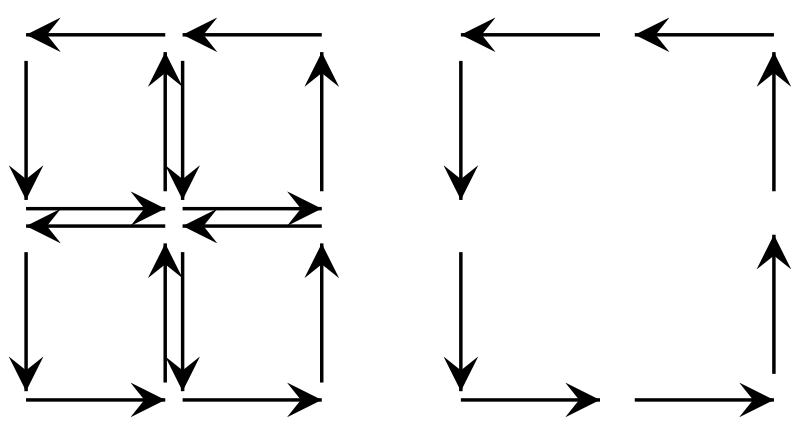
\includegraphics[width=6cm]{media/stokes-patch.png}
		\\ \scriptsize Image from \cite{img:stokes}
	\end{minipage}
\end{center}


\section{Differential forms}
\prototype{Algebraically,
	something that looks like $f \ee_1^\vee \wedge \ee_2^\vee + \dots$,
	and geometrically, see the previous section.}

Let's now get a handle on what $dx$ means.
Fix a real vector space $V$ of dimension $n$,
and let $\ee_1$, \dots, $\ee_n$ be a standard basis.
Let $U$ be an open set.

\begin{definition}
	We define a \vocab{differential $k$-form} $\alpha$ on $U$
	to be a smooth (infinitely differentiable) map
	$\alpha : U \to \Lambda^k(V^\vee)$.
	(Here $\Lambda^k(V^\vee)$ is the wedge product.)
\end{definition}

Like with $Df$, we'll use $\alpha_p$ instead of $\alpha(p)$.

\begin{example}
	[$k$-forms for $k=0,1$]
	\listhack
	\begin{enumerate}[(a)]
		\item A $0$-form is just a function $U \to \RR$.
		\item A $1$-form is a function $U \to V^\vee$.
		For example,
		the total derivative $Df$ of a function $V \to \RR$ is a $1$-form.
		\item Let $V = \RR^3$ with standard basis $\ee_1$, $\ee_2$, $\ee_3$.
		Then a typical $2$-form is given by
		\[
			\alpha_p
			=
			f(p) \cdot \ee_1^\vee \wedge \ee_2^\vee
			+ g(p) \cdot \ee_1^\vee \wedge \ee_3^\vee
			+ h(p) \cdot \ee_2^\vee \wedge \ee_3^\vee
			\in \Lambda^2(V)
		\]
		where $f,g,h : V \to \RR$ are smooth functions.
	\end{enumerate}
\end{example}

Now, by the projection principle (\Cref{thm:project_principle}) we only have to specify
a function on each of $\binom nk$ basis elements of $\Lambda^k(V^\vee)$.
So, take any basis $\{e_i\}$ of $V$, and 
take the usual basis for $\Lambda^k(V^\vee)$ of elements
\[ e_{i_1}^\vee \wedge e_{i_2}^\vee \wedge \dots \wedge e_{i_k}^\vee. \]
Thus, a general $k$-form takes the shape
\[ \alpha_p = \sum_{1 \le i_1 < \dots < i_k \le n} 
	f_{i_1, \dots, i_k}(p) \cdot
	e_{i_1}^\vee \wedge e_{i_2}^\vee \wedge \dots \wedge e_{i_k}^\vee. \]
Since this is a huge nuisance to write, we will abbreviate this to just
\[ \alpha = \sum_I f_I \cdot de_I \]
where we understand the sum runs over $I = (i_1, \dots, i_k)$,
and $de_I$ represents $e_{i_1}^\vee \wedge \dots \wedge e_{i_k}^\vee$.

Now that we have an element $\Lambda^k(V^\vee)$, what can it do?
Well, first let me get the definition on the table, then tell you what it's doing.
\begin{definition}
	For linear functions $\xi_1, \dots, \xi_k \in V^\vee$
	and vectors $v_1, \dots, v_k \in V$, set
	\[
		(\xi_1 \wedge \dots \wedge \xi_k)(v_1, \dots, v_k)
		\defeq
		\det
		\begin{bmatrix}
			\xi_1(v_1) & \dots & \xi_1(v_k) \\
			\vdots & \ddots & \vdots \\
			\xi_k(v_1) & \dots & \xi_k(v_k)
		\end{bmatrix}.
	\]
	You can check that this is well-defined
	under e.g. $v \wedge w = -w \wedge v$ and so on.
\end{definition}

\begin{example}
	[Evaluation of a differential form]
	Set $V = \RR^3$.
	Suppose that at some point $p$, the $2$-form $\alpha$ returns
	\[ \alpha_p = 2 \ee_1^\vee \wedge \ee_2^\vee + \ee_1^\vee \wedge \ee_3^\vee. \]
	Let $v_1 = 3\ee_1 + \ee_2 + 4\ee_3$ and $v_2 = 8\ee_1 + 9\ee_2 + 5\ee_3$.
	Then
	\[
		\alpha_p(v_1, v_2)
		=
		2\det \begin{bmatrix}
			3 & 8 \\ 1 & 9 \end{bmatrix}
		+
		\det \begin{bmatrix}
			3 & 8 \\ 4 & 5 \end{bmatrix}
		= 21.
	\]
\end{example}

What does this definition mean?
One way to say it is that
\begin{moral}
	If I walk to a point $p \in U$,
	a $k$-form $\alpha$ will take in $k$ vectors $v_1, \dots, v_k$
	and spit out a number, which is to be interpreted as a (signed) volume.
\end{moral}

Picture:
\begin{center}
	\begin{asy}
		bigblob("$U$");
		pair p = (-2,-2);
		dot("$p$", p, dir(225), red);
		pair p1 = p + 1.4*dir(120);
		pair p2 = p + 1.7*dir(10);
		draw(p--p1, red, EndArrow);
		draw(p--p2, red, EndArrow);
		label("$v_1$", p1, dir(p1-p), red);
		label("$v_2$", p2, dir(p2-p), red);
		label("$\alpha_p(v_1, v_2) \in \mathbb R$", p+dir(45)*3);
	\end{asy}
\end{center}

In other words, at every point $p$, we get a function $\alpha_p$.
Then I can feed in $k$ vectors to $\alpha_p$ and get a number,
which I interpret as a signed volume of the parallelpiped spanned by the $\{v_i\}$'s
in some way (e.g.\ the flux of a force field).
That's why $\alpha_p$ as a ``function'' is contrived to lie in the wedge product:
this ensures that the notion of ``volume'' makes sense, so that for example,
the equality $\alpha_p(v_1, v_2) = -\alpha_p(v_2, v_1)$ holds.

This is what makes differential forms so fit for integration.


\section{Exterior derivatives}
\prototype{Possibly $dx_1 = \ee_1^\vee$.}
We now define the exterior derivative $df$ that we gave
pictures of at the beginning of the section.
It turns out that the exterior derivative is easy to compute
given explicit coordinates to work with.

First, given a function $f : U \to \RR$,
we define
\[ df \defeq Df = \sum_i \frac{\partial f_i}{\partial e_i} e_i^\vee \]
In particular, suppose $V = \RR^n$ and $f(x_1, \dots, x_n) = x_1$
(i.e.\ $f = \ee_1^\vee$). Then:
\begin{ques}
	Show that for any $p \in U$, \[ \left( d(\ee_1^\vee) \right)_p = \ee_1^\vee. \]
\end{ques}

\begin{abuse}
	Unfortunately, someone somewhere decided
	it would be a good idea to use ``$x_1$'' to denote $\ee_1^\vee$
	(because \emph{obviously}\footnote{Sarcasm.} $x_1$ means
	``the function that takes $(x_1, \dots, x_n) \in \RR^n$ to $x_1$'')
	and then decided that \[ dx_1 \defeq \ee_1^\vee. \]
	This notation is so entrenched that I have no choice
	but to grudgingly accept it.
	Note that it's not even right,
	since technically it's $(dx_1)_p = \ee_1^\vee$; $dx_1$ is a $1$-form.
	\label{abuse:dx}
\end{abuse}
\begin{remark}
	This is the reason why we use the notation $\frac{df}{dx}$ in calculus now:
	given, say, $f : \RR \to \RR$ by $f(x) = x^2$, it is indeed true that
	\[ df = 2x \cdot \ee_1^\vee = 2x \cdot dx \]
	and so by (more) abuse of notation we write $df/dx = 2x$.
\end{remark}

More generally, we can define the \vocab{exterior derivative}
in terms of our basis $e_1$, \dots, $e_n$ as follows:
if $\alpha = \sum_I f_I de_I$ then we set
\[ d\alpha \defeq \sum_I df_I \wedge de_I
	= \sum_I \sum_j \fpartial{f_I}{e_j} de_j \wedge de_I. \]
This doesn't depend on the choice of basis.

\begin{example}[Computing some exterior derivatives]
	Let $V = \RR^3$ with standard basis $\ee_1$, $\ee_2$, $\ee_3$.
	Let $f(x,y,z) = x^4 + y^3 + 2xz$.
	Then we compute
	\[ df = Df = (4x^3+2z) \; dx + 3y^2 \; dy + 2x \; dz. \]
	Next, we can evaluate $d(df)$ as prescribed: it is
	\begin{align*}
		d^2f &= (12x^2 \; dx + 2 dz) \wedge dx + (6y \; dy) \wedge dy
		+ 2(dx \wedge dz) \\
		&= 12x^2 (dx \wedge dx) + 2(dz \wedge dx) + 6y (dy \wedge dy) + 2(dx \wedge dz) \\
		&= 2(dz \wedge dx) + 2(dx \wedge dz) \\
		&= 0.
	\end{align*}
	So surprisingly, $d^2f$ is the zero map.
	Here, we have exploited \Cref{abuse:dx} for the first time,
	in writing $dx$, $dy$, $dz$.
\end{example}
And in fact, this is always true in general:
\begin{theorem}[Exterior derivative vanishes]
	\label{thm:dd_zero}
	Let $\alpha$ be any $k$-form.
	Then $d^2(\alpha) = 0$.
	Even more succinctly, \[ d^2 = 0. \]
\end{theorem}
The proof is left as \Cref{prob:dd_zero}.
\begin{exercise}
	Compare the statement $d^2 = 0$ to the geometric
	picture of a $2$-form given at the beginning of this chapter.
	Why does this intuitively make sense?
\end{exercise}

Here are some other properties of $d$:
\begin{itemize}
	\ii As we just saw, $d^2 = 0$.
	\ii For a $k$-form $\alpha$ and $\ell$-form $\beta$, one can show that
	\[ d(\alpha \wedge \beta) = d\alpha \wedge \beta + (-1)^k (\alpha \wedge d\beta). \]
	\ii If $f \colon U \to \RR$ is smooth, then $df = Df$.
\end{itemize}
In fact, one can show that $df$ as defined above is
the \emph{unique} map sending $k$-forms to $(k+1)$-forms
with these properties.
So, one way to define $df$ is to take as axioms
the bulleted properties above
and then declare $d$ to be the unique solution to this functional equation.
In any case, this tells us that our definition of $d$
does not depend on the basis chosen.

Recall that $df$ measures the change in boundary.
In that sense, $d^2 = 0$ is saying something like
``the boundary of the boundary is empty''.
We'll make this precise when we see Stokes' theorem in the next chapter.

\section{Closed and exact forms}
Let $\alpha$ be a $k$-form.
\begin{definition}
	We say $\alpha$ is \vocab{closed} if $d\alpha = 0$.
\end{definition}
\begin{definition}
	We say $\alpha$ is \vocab{exact} if for some $(k-1)$-form $\beta$,
	$d\beta = \alpha$.  If $k = 0$, $\alpha$ is exact only when $\alpha = 0$.
\end{definition}
\begin{ques}
	Show that exact forms are closed.
\end{ques}

A natural question arises: are there closed forms
which are not exact?
Surprisingly, the answer to this question is tied to topology.
Here is one important example.

\begin{example}
	[The angle form]
	\label{ex:angle_form}
	Let $U = \RR^2 \setminus \{0\}$,
	and let $\theta(p)$ be the angle formed by the $x$-axis
	and the line from the origin to $p$.

	The $1$-form $\alpha : U \to (\RR^2)^\vee$ defined by
	\[ \alpha = \frac{-y \; dx + x \; dy}{x^2+y^2} \]
	is called the \vocab{angle form}:
	given $p \in U$ it measures the change in angle $\theta(p)$
	along a tangent vector.
	So intuitively, ``$\alpha = d\theta$''.
	Indeed, one can check directly that the angle form is closed.

	However, $\alpha$ is not exact: there is no global smooth
	function $\theta : U \to \RR$ having $\alpha$ as a derivative.
	This reflects the fact that one can actually perform
	a full $2\pi$ rotation around the origin, i.e.\ $\theta$
	only makes sense mod $2\pi$.
	Thus existence of the angle form $\alpha$ reflects
	the possibility of ``winding'' around the origin.
\end{example}

So the key idea is that the failure of a closed form to be exact
corresponds quite well with ``holes'' in the space:
the same information that homotopy and homology groups are trying to capture.
To draw another analogy, in complex analysis Cauchy-Goursat
only works when $U$ is simply connected.
The ``hole'' in $U$ is being detected by the existence of a form $\alpha$.
The so-called de Rham cohomology will make this relation explicit.

\section\problemhead
\begin{problem}
	Show directly that the angle form
	\[ \alpha = \frac{-y \; dx + x \; dy}{x^2+y^2} \]
	is closed.
\end{problem}
  
\begin{problem}
	\label{prob:dd_zero}
	Establish \Cref{thm:dd_zero}, which states that $d^2 = 0$.
	\begin{hint}
		This is just a summation.
		You will need the fact that mixed partials are symmetric.
	\end{hint}
\end{problem}

\chapter{Integrating differential forms}
We now show how to integrate differential forms over cells,
and state Stokes' theorem in this context.
In this chapter, all vector spaces are finite-dimensional and real.

\section{Motivation: line integrals}
Given a function $g : [a,b] \to \RR$,
we know by the fundamental theorem of calculus that
\[
	\int_{[a,b]} g(t) \; dt = f(b) - f(a)
\]
where $f$ is a function such that $g = df/dt$.
%(You might recognize this more readily
%as the more customary $\int_a^b g(t) \; dt$.)
Equivalently, for $f : [a,b] \to \RR$,
\[ \int_{[a,b]} g \; dt = \int_{[a,b]} df = f(b) - f(a) \]
where $df$ is the exterior derivative we defined earlier.

Cool, so we can integrate over $[a,b]$.
Now suppose more generally, we have $U$ an open subset of our real vector space $V$
and a $1$-form $\alpha : U \to V^\vee$.
We consider a \vocab{parametrized curve}, which is a smooth function $c : [a,b] \to U$.
Picture:
\begin{center}
	\begin{asy}
		size(8.5cm);
		pair A = (-13,0);
		pair B = (-9,0);
		draw(A--B, grey);
		dot(A, grey); dot(B, grey);
		label("$[a,b]$", A--B, dir(90), grey);
		dot("$t$", 0.3*A+0.7*B, dir(-90), grey);

		draw( (-8,0) -- (-6,0) , EndArrow);
		label("$c$", (-7,0), dir(90));

		bigblob("$U$");
		pair a = (-2,-2);
		pair b = (3,0);
		pair p = (0,1);
		pair q = (2,0);
		label("$c$", q, dir(45), red);
		draw(a..p..q..b, red);
		dot("$p = c(t)$", p, dir(90), blue);
		draw(p--(p+1.5*dir(-10)), blue, EndArrow);

		draw( (0,-4)--(0,-8), EndArrow );
		label("$\alpha$", (0,-6), dir(0));
		label("$\alpha_p(v) \in \mathbb R$", (0,-9), heavygreen);

		draw( (-10,-1)--(-1,-8), EndArrow);
		label("$c^\ast \alpha$", (-5.5,-4.5), dir(225));
	\end{asy}
\end{center}

We want to define an $\int_c \alpha$ such that:
\begin{moral}
	The integral $\int_c \alpha$ should add up all the $\alpha$ along the curve $c$.
\end{moral}
Our differential form $\alpha$ first takes in a point $p$ to get $\alpha_p \in V^\vee$.
Then, it eats a tangent vector $v \in V$ to the curve $c$ to finally give a real number $\alpha_p(v) \in \RR$.
We would like to ``add all these numbers up'',
using only the notion of an integral over $[a,b]$.

\begin{exercise}
	Try to guess what the definition of the integral should be.
	(By type-checking, there's only one reasonable answer.)
\end{exercise}

So, the definition we give is
\[ \int_c \alpha \defeq
	\int_{[a,b]} \alpha_{c(t)} \left( c'(t) \right) \; dt.  \]
Here, $c'(t)$ is shorthand for $(Dc)_{c(t)}(1)$.
It represents the \emph{tangent vector} to the curve $c$ at the point $p=c(t)$,
at time $t$.
(Here we are taking advantage of the fact that $[a,b]$ is one-dimensional.)

Now that definition was a pain to write, so we will define a differential
$1$-form $c^\ast \alpha$ on $[a,b]$ to swallow that entire thing:
specifically, in this case we define $c^\ast\alpha$ to be
\[ \left( c^\ast \alpha \right)_t (\eps) = \alpha_{c(t)} \cdot (Dc)_{t} (\eps) \]
(here $\eps$ is some displacement in time).
Thus, we can more succinctly write
\[ \int_c \alpha \defeq \int_{[a,b]} c^\ast \alpha. \]
This is a special case of a \emph{pullback}:
roughly, if $\phi : U \to U'$ (where $U \subseteq V$, $U' \subseteq V'$),
we can change any differential $k$-form $\alpha$ on $U'$
to a $k$-form on $U$.
In particular, if $U = [a,b]$,\footnote{OK,
	so $[a,b]$ isn't actually open, sorry.
	I ought to write $(a-\eps, b+\eps)$, or something.}
we can resort to our old definition of an integral.
Let's now do this in full generality.

\section{Pullbacks}
Let $V$ and $V'$ be finite dimensional real vector spaces (possibly different dimensions)
and suppose $U$ and $U'$ are open subsets of each;
next, consider a $k$-form $\alpha$ on $U'$.

Given a map $\phi : U \to U'$ we now want to define a pullback in
much the same way as before.
Picture:
\begin{center}
	\begin{asy}
		size(13cm);
		bigblob("$U$");
		pair p = (-1,0);
		dot("$p$", p, dir(90), red);
		pair p1 = p + 1.4*dir(150);
		pair p2 = p + 1.7*dir(-50);
		draw(p--p1, red, EndArrow);
		draw(p--p2, red, EndArrow);

		add(scale(0.8)*shift(14*dir(180))*CC());
		bigblob("$U'$");
		pair q = (-0.5,0.5);
		dot("$q = \phi(p)$", q, dir(90), blue);
		pair q1 = q + 1.8*dir(-100);
		pair q2 = q + 2.3*dir(-10);
		draw(q--q1, blue, EndArrow);
		draw(q--q2, blue, EndArrow);

		draw((-9,0)--(-3,0), EndArrow);
		label("$\phi$", (-6,0), dir(90));
	
		draw( (0,-4)--(0,-8), EndArrow );
		label("$\alpha$", (0,-6), dir(0));
		label("$\alpha_q(\dots) \in \mathbb R$", (0,-9), heavygreen);

		draw( (-11,-3)--(-1,-8), EndArrow);
		label("$\phi^\ast \alpha$", (-6,-6), dir(225));
	\end{asy}
\end{center}

Well, there's a total of about one thing we can do.
Specifically: $\alpha$ accepts a point in $U'$ and $k$ tangent vectors in $V'$,
and returns a real number.
We want $\phi^\ast \alpha$ to accept a point in $p \in U$
and $k$ tangent vectors $v_1, \dots, v_k$ in $V$,
and feed the corresponding information to $\alpha$.

Clearly we give the point $q = \phi(p)$.
As for the tangent vectors, since we are interested in volume, we take the
derivative of $\phi$ at $p$, $(D\phi)_p$, which will scale each of our vectors $v_i$
into some vector in the target $V'$.
To cut a long story short:
\begin{definition}
	Given $\phi : U \to U'$ and $\alpha$ a $k$-form, we define the \vocab{pullback}
	\[
		(\phi^\ast \alpha)_p(v_1, \dots, v_k)
		\defeq \alpha_{\phi(p)}
		\left( (D\phi)_p(v_1), \dots, (D\phi)_p(v_k) \right).
	\]
\end{definition}

There is a more concrete way to define the pullback using bases.
Suppose $w_1, \dots, w_n$ is a basis of $V'$
and $e_1, \dots, e_m$ is a basis of $V$.
Thus, by the projection principle (\Cref{thm:project_principle}) 
the map $\phi : V \to V'$ can be thought of as
\[ \phi(v) = \phi_1(v) w_1 +  \dots \phi_n(v) w_n \]
where each $\phi_i$ takes in a $v \in V$ and returns a real number.
We know also that $\alpha$ can be written concretely as
\[ \alpha = \sum_{J \subseteq \{1, \dots, n\}} f_J w_J. \]
Then, we define
\[
	\phi^\ast\alpha
	= \sum_{I \subseteq \{1, \dots, m\}}
	(f_I \circ \phi) (D\phi_{i_1} \wedge \dots \wedge D\phi_{i_k}).
\]
A diligent reader can check these definitions are equivalent.
\begin{example}
	[Computation of a pullback]
	Let $V = \RR^2$ with basis $\ee_1$ and $\ee_2$,
	and suppose $\phi : V \to V'$ is given by sending
	\[ \phi(a\ee_1 + b\ee_2) = (a^2+b^2)w_1 + \log(a^2+1) w_2 + b^3 w_3 \]
	where $w_1$, $w_2$, $w_3$ is a basis for $V'$.
	Consider the form $\alpha_q = f(q) w_1 \wedge w_3$, where $f : V' \to \RR$.
	Then
	\[ (\phi^\ast\alpha)_p = f(\phi(p)) \cdot (2a \ee_1^\vee + 2b\ee_2^\vee) \wedge (3b^2 \ee_2^\vee)
		= f(\phi(p)) \cdot 6ab^2 \cdot \ee_1^\vee \wedge \ee_2^\vee. \]
\end{example}

It turns out that the pullback basically behaves nicely as possible, e.g.\
\begin{itemize}
	\ii $\phi^\ast(c\alpha + \beta) = c\phi^\ast \alpha + \phi^\ast\beta$ (linearity)
	\ii $\phi^\ast(\alpha\wedge\beta)
	= (\phi^\ast \alpha)\wedge(\phi^\ast \beta)$
	\ii $\phi_1^\ast(\phi_2^\ast(\alpha)) 
	= (\phi_2 \circ \phi_1)^\ast(\alpha)$ (naturality)
\end{itemize}
but I won't take the time to check these here
(one can verify them all by expanding with a basis).
	
\section{Cells}
\prototype{A disk in $\RR^2$ can be thought of as the cell
	$[0,R]\times[0,2\pi] \to \RR^2$ by
	$(r,\theta) \mapsto (r\cos\theta)\ee_1 + (r\sin\theta)\ee_2$.}
Now that we have the notion of a pullback,
we can define the notion of an integral for more general spaces.
Specifically, to generalize the notion of integrals we had before:
\begin{definition}
	A \vocab{$k$-cell} is a smooth function $c : [a_1, b_1] \times [a_2,b_2] \times \dots [a_k, b_k] \to V$.
\end{definition}
\begin{example}
	[Examples of cells]
	Let $V = \RR^2$ for convenience.
	\begin{enumerate}[(a)]
		\ii A $0$-cell consists of a single point.
		\ii As we saw, a $1$-cell is an arbitrary curve.
		\ii A $2$-cell corresponds to a $2$-dimensional surface.
		For example, the map $c : [0,R] \times [0,2\pi] \to V$ by
		\[ c : (r,\theta) \mapsto (r\cos\theta, r\sin\theta) \]
		can be thought of as a disk of radius $R$.
	\end{enumerate}
\end{example}
Then, to define an integral
\[ \int_c \alpha \]
for a differential $k$-form $\alpha$ and a $k$-cell $c : [0,1]^k \to V$,
we simply take the pullback
\[ \int_{[0,1]^k} c^\ast \alpha \]
Since $c^\ast \alpha$ is a $k$-form on the $k$-dimensional unit box,
it can be written as $f(x_1, \dots, x_n) \; dx_1 \wedge \dots \wedge dx_n$,
so the above integral can be written as
\[ \int_0^1 \dots \int_0^1 f(x_1, \dots, x_n) \; dx_1 \wedge \dots \wedge dx_n \]

\begin{example}[Area of a circle]
	Consider $V = \RR^2$ and let $c : (r,\theta) \mapsto (r\cos\theta)\ee_1 + (r\sin\theta)\ee_2$
	on $[0,R] \times [0,2\pi]$ as before.
	Take the $2$-form $\alpha$ which gives $\alpha_p = \ee_1^\vee \wedge \ee_2^\vee$ at every point $p$.
	Then
	\begin{align*}
		c^\ast\alpha &= 
		\left( \cos\theta dr - r\sin\theta d\theta \right)
		\wedge
		\left( \sin\theta dr + r\cos\theta d\theta \right) \\
		&= r(\cos^2\theta+\sin^2\theta) (dr \wedge d\theta) \\
		&= r \; dr \wedge d\theta
	\end{align*}
	Thus,
	\[ \int_c \alpha
		= \int_0^R \int_0^{2\pi} r \; dr \wedge d\theta
		= \pi R^2 \]
	which is the area of a circle.
\end{example}

Here's some geometric intuition for what's happening.
Given a $k$-cell in $V$, a differential $k$-form $\alpha$ accepts a point $p$ and some tangent vectors $v_1$, \dots, $v_k$
and spits out a number $\alpha_p(v_1, \dots, v_k)$,
which as before we view as a signed hypervolume.
Then the integral \emph{adds up all these infinitesimals across the entire cell}.
In particular, if $V = \RR^k$ and we take the form $\alpha : p \mapsto \ee_1^\vee \wedge \dots \wedge \ee_k^\vee$,
then what these $\alpha$'s give is the $k$th hypervolume of the cell.
For this reason, this $\alpha$ is called the \vocab{volume form} on $\RR^k$.

You'll notice I'm starting to play loose with the term ``cell'':
while the cell $c : [0,R] \times [0,2\pi] \to \RR^2$ is supposed to be a function
I have been telling you to think of it as a unit disk (i.e.\ in terms of its image).
In the same vein, a curve $[0,1] \to V$ should be thought of as a curve in space,
rather than a function on time.

This error turns out to be benign.
Let $\alpha$ be a $k$-form on $U$ and $c : [a_1, b_1] \times \dots \times [a_k, b_k] \to U$ a $k$-cell.
Suppose $\phi : [a_1', b_1'] \times \dots [a_k', b_k'] \to [a_1, b_1] \times \dots \times [a_k, b_k]$;
it is a \vocab{reparametrization} if $\phi$ is bijective and $(D\phi)_p$ is always invertible
(think ``change of variables'');
thus
\[ c \circ \phi : [a_1', b_1'] \times \dots \times [a_k',b_k'] \to U \]
is a $k$-cell as well.
Then it is said to \vocab{preserve orientation} if $\det(D\phi)_p > 0$ for all $p$
and \vocab{reverse orientation} if $\det(D\phi)_p < 0$ for all $p$.
\begin{exercise}
	Why is it that exactly one of these cases must occur?
\end{exercise}

\begin{theorem}
	[Changing variables doesn't affect integrals]
	Let $c$ be a $k$-cell, $\alpha$ a $k$-form, and $\phi$ a reparametrization.
	Then
	\[ \int_{c \circ \phi} \alpha
		=
		\begin{cases}
			\int_c \alpha & \phi \text{ preserves orientation} \\
			- \int_c \alpha & \phi \text{ reverses orientation}.
		\end{cases}
	\]
\end{theorem}
\begin{proof}
	Use naturality of the pullback to reduce it to the corresponding
	theorem in normal calculus.
\end{proof}

So for example, if we had parametrized the unit circle as $[0,1] \times [0,1] \to \RR^2$
by $(r,t) \mapsto R\cos(2\pi t) \ee_1 + R\sin(2\pi t) \ee_2$, we would have arrived at the same result.
So we really can think of a $k$-cell just in terms of the points it specifies.

\section{Boundaries}
\prototype{The boundary of $[a,b]$ is $\{b\}-\{a\}$. The boundary of a square goes around its edge counterclockwise.}
First, I introduce a technical term that lets us consider multiple cells at once.
\begin{definition}
	A \vocab{$k$-chain} $U$ is a formal
	linear combination of $k$-cells over $U$,
	i.e.\ a sum of the form
	\[ c = a_1 c_1 + \dots + a_m c_m \]
	where each $a_i \in \RR$ and $c_i$ is a $k$-cell.
	We define $\int_c \alpha = \sum_i a_i \int c_i$.
\end{definition}
In particular, a $0$-chain consists of several points, each with a given weight.

Now, how do we define the boundary?
For a $1$-cell $[a,b] \to U$, as I hinted earlier we want the answer to be the $0$-chain $\{c(b)\}-\{c(a)\}$.
Here's how we do it in general.
\begin{definition}
	Suppose $c : [0,1]^k \to U$ is a $k$-cell.
	Then the \vocab{boundary} of $c$, denoted $\partial c : [0,1]^{k-1} \to U$,
	is the $(k-1)$-chain defined as follows.
	For each $i = 1,\dots,k$ define
	\begin{align*}
		c_i^{\text{start}}(t_1, \dots, t_{k-1}) &
		= (t_1, \dots, t_{i-1}, 0, t_i, \dots, t_k) \\
		c_i^{\text{stop}}(t_1, \dots, t_{k-1}) &
		= (t_1, \dots, t_{i-1}, 1, t_i, \dots, t_k).
	\end{align*}
	Then
	\[ \partial c \defeq
	\sum_{i=1}^k (-1)^{i+1} \left( c_i^{\text{stop}} - c_i^{\text{start}}  \right). \]
	Finally, the boundary of a chain is the sum of the boundaries of each cell (with the appropriate weights).
	That is, $\partial(\sum a_ic_i) = \sum a_i \partial c_i$.
\end{definition}
\begin{ques}
	Satisfy yourself that one can extend this definition to
	a $k$-cell $c$ defined on $c : [a_1, b_1] \times \dots \times [a_k, b_k] \to V$
	(rather than from $[0,1]^k \to V$).
\end{ques}

\begin{example}
	[Examples of boundaries]
	Consider the $2$-cell $c : [0,1]^2 \to \RR^2$ shown below.
	\begin{center}
		\begin{asy}
			size(7cm);
			pen e1 = heavyred;
			pen e2 = orange;
			pen e3 = olive;
			pen e4 = heavymagenta;
			draw((0,0)--(2,0), e1, EndArrow);
			draw((2,0)--(2,2), e2, EndArrow);
			draw((2,2)--(0,2), e3, EndArrow);
			draw((0,2)--(0,0), e4, EndArrow);
			label(scale(0.8)*"$[0,1]^2$", (1,1));
			draw( (3,1)--(6,1), EndArrow);
			label("$c$", (4.5,1), dir(90));
			pair p1 = (7,-1);
			pair p2 = (12,-2);
			pair p3 = (11,3);
			pair p4 = (8,2);
			fill(p1--p2--p3--p4--cycle, palecyan);
			draw(p1--p2, e1, EndArrow, Margins);
			draw(p2--p3, e2, EndArrow, Margins);
			draw(p3--p4, e3, EndArrow, Margins);
			draw(p4--p1, e4, EndArrow, Margins);
			dot("$p_1$", p1, dir(225), blue+4);
			dot("$p_2$", p2, dir(315), blue+4);
			dot("$p_3$", p3, dir( 45), blue+4);
			dot("$p_4$", p4, dir(135), blue+4);
			label("$c$", (p1+p2+p3+p4)/4);
		\end{asy}
	\end{center}
	Here $p_1$, $p_2$, $p_3$, $p_4$ are the images of $(0,0)$, $(0,1)$, $(1,0)$, $(1,1)$, respectively.
	Then we can think of $\partial c$ as
	\[ \partial c = [p_1,p_2] + [p_2,p_3] + [p_3,p_4] + [p_4,p_1] \]
where each ``interval'' represents the $1$-cell shown by the reddish arrows on the right.
	We can take the boundary of this as well, and obtain an empty chain as
	\[ \partial(\partial c) = \sum_{i=1}^4 \partial([p_i, p_{i+1}]) = \sum_{i=1}^4 \{p_{i+1}\}-\{p_i\} = 0. \]
\end{example}

\begin{example}
	[Boundary of a unit disk]
	Consider the unit disk given by
	\[ c : [0,1] \times [0,2\pi] \to \RR^2 \quad\text{by}\quad
	(r,\theta) \mapsto s\cos(2\pi t)\ee_1 + s\sin(2\pi t)\ee_2. \]
	The four parts of the boundary are shown in the picture below:
	\begin{center}
		\begin{asy}
			size(7cm);
			pen e1 = heavyred;
			pen e2 = orange;
			pen e3 = olive;
			pen e4 = heavymagenta;
			draw((0,0)--(2,0), e1, EndArrow);
			draw((2,0)--(2,2), e2, EndArrow);
			draw((2,2)--(0,2), e3, EndArrow);
			draw((0,2)--(0,0), e4, EndArrow);
			label("$r$", (2,0), dir(-45));
			label("$\theta$", (0,2), dir(135));

			label(scale(0.8)*"$[0,1]^2$", (1,1));
			draw( (3,1)--(6,1), EndArrow);
			label("$c$", (4.5,1), dir(90));

			pair O = (9,1);
			pair P = O + 2*dir(0);
			fill(CP(O,P), palecyan);
			real eps = 0.3;
			draw(shift(0,eps) * (O--P), e1, EndArrow, Margins);
			draw(shift(0,-eps) * (P--O), e3, EndArrow, Margins);
			draw(CP(O,P), e2, EndArrow, Margins);
			dot(O, e4+4);
		\end{asy}
	\end{center}
	Note that two of the arrows more or less cancel each other out when they are integrated.
	Moreover, we interestingly have a \emph{degenerate} $1$-cell at the center of the circle;
	it is a constant function $[0,1] \to \RR^2$ which always gives the origin.
\end{example}

Obligatory theorem, analogous to $d^2=0$ and left as a problem.
\begin{theorem}[The boundary of the boundary is empty]
	$\partial^2 = 0$, in the sense that for any $k$-chain $c$ we have $\partial^2(c) = 0$.
\end{theorem}

\section{Stokes' theorem}
\prototype{$\int_{[a,b]} dg = g(b) - g(a)$.}

We now have all the ingredients to state Stokes' theorem for cells.
\begin{theorem}
	[Stokes' theorem for cells]
	Take $U \subseteq V$ as usual, let $c : [0,1]^k \to U$ be a $k$-cell
	and let $\alpha : U \to \Lambda^{k-1}(V^\vee)$ be a $k-1$-form.
	Then
	\[ \int_c d\alpha = \int_{\partial c} \alpha. \]
	In particular, if $d\alpha = 0$ then the left-hand side vanishes.
\end{theorem}
For example, if $c$ is the interval $[a,b]$ then $\partial c = \{b\} - \{a\}$,
and thus we obtain the fundamental theorem of calculus.

\section\problemhead
\begin{dproblem}[Green's theorem]
	Let $f,g : \RR^2 \to \RR$ be smooth functions.
	Prove that
	\[ \int_c \left( \fpartial gx - \fpartial fy \right) \; dx \wedge dy
	= \int_{\partial c} (f \; dx + g \; dy). \]
	\begin{hint}
		Direct application of Stokes' theorem to $\alpha = f \; dx + g \; dy$.
	\end{hint}
\end{dproblem}

\begin{problem}
	Show that $\partial^2 = 0$.
	\label{prob:partial_zero}
	\begin{hint}
		This is just an exercises in sigma notation.
	\end{hint}
\end{problem}

\begin{problem}[Pullback and $d$ commute]
	Let $U$ and $U'$ be open sets of vector spaces $V$ and $V'$
	and let $\phi : U \to U'$ be a smooth map between them.
	Prove that for any differential form $\alpha$ on $U'$ we have
	\[ \phi^\ast(d\alpha) = d(\phi^\ast\alpha). \]
	\begin{hint}
		This is a straightforward (but annoying) computation.
	\end{hint}
\end{problem}

\begin{problem}[Arc length isn't a form]
	Show that there does \emph{not} exist a $1$-form $\alpha$ on $\RR^2$ such that
	for a curve $c : [0,1] \to \RR^2$,
	the integral $\int_c \alpha$ gives the arc length of $c$.
	\begin{hint}
		We would want $\alpha_p(v) = \norm{v}$.
	\end{hint}
\end{problem}

\begin{problem}
	An \vocab{exact} $k$-form $\alpha$ is one satisfying $\alpha = d\beta$ for some $\beta$.
	Prove that
	\[ \int_{C_1} \alpha = \int_{C_2} \alpha \]
	where $C_1$ and $C_2$ are any concentric circles in the plane
	and $\alpha$ is some exact $1$-form.
	\begin{hint}
		Show that $d^2=0$ implies $\int_{\partial c} \alpha = 0$ for exact $\alpha$.
		Draw an annulus.
	\end{hint}
\end{problem}
 % sols
\chapter{Manifolds}


\part{Algebraic Topology II: Homology}
\chapter{Singular homology}
Now that we've defined $\pi_1(X)$,
we turn our attention to a second way of capturing the same idea, $H_1(X)$.
We'll then define $H_n(X)$ for $n \ge 2$.
The good thing about the $H_n$ groups is that, unlike the $\pi_n$ groups,
they are much easier to compute in practice.
The downside is that their definition will require quite a bit of setup,
and the ``algebraic'' part of ``algebraic topology'' will become a lot more technical.

\section{Simplices and boundaries}
\prototype{$\partial[v_0, v_1, v_2] = [v_0,v_1]-[v_0,v_2]+[v_1,v_2]$.}
First things first:
\begin{definition}
	The \vocab{standard $n$-simplex}, denoted $\Delta^n$, is defined as
	\[ \left\{ (x_0 , x_1, \dots x_n) \mid x_i \ge 0, x_0+\dots+x_n=1 \right\}. \]
	Hence it's the convex hull of some vertices $[v_0, \dots, v_n]$.
	Note that we keep track of the order $v_0$, \dots, $v_n$ of the vertices,
	for reasons that will soon become clear.

	Given a topological space $X$, a \vocab{singular $n$-simplex} is a map $\sigma : \Delta^n \to X$.
\end{definition}
\begin{example}
	[Singular simplices]
	\listhack
	\label{ex:simplex}
	\begin{enumerate}[(a)]
		\ii Since $\Delta^0 = [v_0]$ is just a point,
		a singular $0$-simplex $X$ is just a point of $X$.
		\ii Since $\Delta^1 = [v_0, v_1]$ is an interval,
		a singular $1$-simplex $X$ is just a path in $X$.
		\ii Since $\Delta^2 = [v_0, v_1, v_2]$ is an equilateral triangle,
		a singular $2$-simplex $X$ looks a ``disk'' in $X$.
	\end{enumerate}
	Here is a picture of all three in a space $X$:
	\begin{center}
		\begin{asy}
			size(8cm);
			bigblob("$X$");
			dot("$\sigma^0$", (-3.7,2.5), dir(-90));

			pen hg = heavygreen;
			pair A0 = (-2.7, 1.1);
			pair A1 = (-2.9, -2.3);
			dot("$v_0$", A0, dir(90), hg);
			dot("$v_1$", A1, dir(-90), hg);
			path s1 = A0..(-3.1,0.7)..A1;
			draw(s1, hg, EndArrow);
			label("$\sigma^1$", s1, dir(10), hg);

			pen rr = red;
			pair B0 = (1, 1.8);
			pair B1 = (-0.7, -1.1);
			pair B2 = (1.9, -1.9);
			dot("$v_0$", B0, dir(90), rr);
			dot("$v_1$", B1, dir(210), rr);
			dot("$v_2$", B2, dir(330), rr);
			pair b0 = (0,0);
			pair b1 = (0,-2);
			pair b2 = (1.6,0.3);
			draw(B0..b0..B1, rr, EndArrow);
			draw(B1..b1..B2, rr, EndArrow);
			draw(B2..b2..B0, rr, EndArrow);
			fill(B0..b0..B1--B1..b1..B2--B2..b2..B0--cycle, lightred+opacity(0.2));
			label("$\sigma^2$", (B0+B1+B2)/3, rr);
		\end{asy}
	\end{center}
	The arrows aren't strictly necessary, but I've included them
	to help keep track of the ``order'' of the vertices;
	this will be useful in just a moment.
\end{example}

Now we're going to do something much like
when we were talking about Stokes' theorem:
we'll put a boundary $\partial$ operator on the singular $n$-simplices.
This will give us a formal linear sums of $n$-simplices $\sum_k a_k \sigma_k$,
which we call an \vocab{$n$-chain}.

In that case,
\begin{definition}
	Given a singular $n$-simplex $\sigma$ with vertices $[v_0, \dots, v_n]$,
	note that for every $i$ we have an $(n-1)$ simplex $[v_0, \dots, v_{i-1}, v_{i+1}, \dots, v_n]$.
	The \vocab{boundary operator} $\partial$ is then defined by
	\[ \partial(\sigma) \defeq \sum_i (-1)^i
		\left[ v_0, \dots, v_{i-1}, v_{i+1}, \dots, v_n \right]. \]
	The boundary operator then extends linearly to $n$-chains:
	\[ \partial\left( \sum_k a_k \sigma_k \right) \defeq \sum a_k \partial(\sigma_k). \]
	By convention, a $0$-chain has empty boundary.
\end{definition}
\begin{example}
	[Boundary operator]
	Consider the chains depicted in \Cref{ex:simplex}. Then
	\begin{enumerate}[(a)]
		\ii $\partial\sigma^0 = 0$.
		\ii $\partial(\sigma^1) = [v_1] - [v_0]$:
		it's the ``difference'' of the $0$-chain corresponding to point $v_1$
		and the $0$-chain corresponding to point $v_0$.
		\ii $\partial(\sigma^2) = [v_0,v_1] - [v_0,v_2] + [v_1, v_2]$;
		i.e.\ one can think of it as the sum of the three oriented arrows
		which make up the ``sides'' of $\sigma^2$.
		\ii Notice that if we take the boundary again, we get
		\begin{align*}
			\partial(\partial(\sigma^2))
			&= \partial([v_0,v_1]) - \partial([v_0,v_2]) + \partial([v_1,v_2]) \\
			&= \left( [v_1]-[v_0] \right) - \left( [v_2]-[v_0] \right) + \left( [v_2]-[v_1] \right)  \\
			&= 0.
		\end{align*}
	\end{enumerate}
\end{example}

The fact that $\partial^2 = 0$ is of course not a coincidence.
\begin{theorem}
	[$\partial^2=0$]
	For any chain $c$, $\partial(\partial(c)) = 0$.
\end{theorem}
\begin{proof}
	Essentially identical to \Cref{prob:partial_zero}:
	this is just a matter of writing down a bunch of $\sum$ signs.
	Diligent readers are welcome to try the computation.
\end{proof}
\begin{remark}
	The eerie similarity between the chains used to integrate differential forms
	and the chains in homology is not a coincidence.
	The de Rham cohomology, discussed much later, will make the relation explicit.
\end{remark}

\section{The singular homology groups}
\prototype{Probably $H_n(S^m)$, especially the case $m = n =1$.}
Let $X$ be a topological space, and let $C_n(X)$ be the free abelian group
of $n$-chains of $X$ that we defined earlier.
Our work above gives us a boundary operator $\partial$, so we have a sequence of maps
\[ \dots \taking\partial C_3(X) \taking\partial C_2(X)
	\taking\partial C_1(X) \taking\partial C_0(X) \taking\partial 0 \]
(here I'm using $0$ to for the trivial group, which is standard notation for abelian groups.)
We'll call this the \vocab{singular chain complex}.

Now, how does this let us detect holes in the space?
To see why, let's consider an annulus, with a $1$-chain $c$ drawn in red:
\begin{center}
	\begin{asy}
		size(6cm);
		pair O = origin;
		filldraw(CR(O, 6), lightblue+opacity(0.2), blue);
		filldraw(CR(O, 1), white, blue);
		label("$X$", 6*dir(45), dir(45));
		pen rr = red;
		pair v0 = 5*dir(100);
		pair v1 = 4*dir(220);
		pair v2 = 2.2*dir(330);
		dot("$v_0$", v0, dir(v0), rr);
		dot("$v_1$", v1, dir(v1), rr);
		dot("$v_2$", v2, dir(v2), rr);
		draw(v0..(3.2*dir(110))..v1, rr, EndArrow);
		draw(v1..(2.1*dir(270))..v2, rr, EndArrow);
		draw(v2..(3.6*dir(45))..v0, rr, EndArrow);
	\end{asy}
\end{center}
Notice that 
\[ \partial c = ([v_1]-[v_0]) - ([v_2]-[v_0]) + ([v_2]-[v_1]) = 0 \]
and so we can say this $1$-chain $c$ is a ``cycle'',
because it has trivial boundary.
However, $c$ is not itself the boundary of any $2$-chain,
because of the hole in the center of the space
--- it's impossible to ``fill in'' the interior of $c$!
So, we have detected the hole by the algebraic fact that 
\[ c \in \ker\left( C_1(X) \taking{\partial} C_0(X) \right)
	\qquad\text{but}\qquad
	c \notin \img \left( C_2(X) \taking{\partial} C_1(X) \right). \]
Indeed, if the hole was not present then this statement would be false.

We can capture this idea in any dimension, as follows.
\begin{definition}
	Let 
	\[ \dots \taking\partial C_2(X) \taking\partial C_1(X) \taking\partial C_0(X) \taking\partial 0 \]
	as above.
	We say that $c \in C_n(X)$ is:
	\begin{itemize}
		\ii a \vocab{cycle} if $c \in \ker\left( C_{n}(X) \taking\partial C_{n-1}(X) \right)$,
		and
		\ii a \vocab{boundary} if $c \in \img \left( C_{n+1}(X) \taking\partial C_n(X) \right)$.
	\end{itemize}
	Denote the cycles and boundaries by $Z_n(X), B_n(X) \subseteq C_n(X)$, respectively.
\end{definition}

\begin{ques}
	Just to get you used to the notation:
	check that $B_n$ and $Z_n$ are themselves abelian groups,
	and that $B_n(X) \subseteq Z_n(X) \subseteq C_n(X)$.
\end{ques}

The key point is that we can now define:
\begin{definition}
	The \vocab{$n$th homology group} $H_n(X)$ is
	defined as \[ H_n(X) \defeq Z_n(X) / B_n(X). \]
\end{definition}
\begin{example}
	[The zeroth homology group]
	Let's compute $H_0(X)$ for a topological space $X$.
	We take $C_0(X)$, which is just formal linear sums of points of $X$.

	First, we consider the kernel of $\partial : C_0(X) \to 0$,
	so the kernel of $\partial$ is the entire space $C_0(X)$:
	that is, every point is a ``cycle''.

	Now, what is the boundary?
	The main idea is that $[b] - [a] = 0$ if and only if
	there's a $1$-chain which connects $a$ to $b$, i.e.\
	there is a path from $a$ to $b$.
	In particular,
	\[ \text{$X$ path connected} \implies H_0(X) \cong \ZZ. \]
\end{example}
More generally, we have
\begin{proposition}[Homology groups split into path-connected components]
	If $X = \bigcup_\alpha X_\alpha$ is a decomposition into path-connected components,
	then we have \[ H_n(X) \cong \bigoplus_\alpha H_n(X_\alpha). \]
	In particular, if $X$ has $r$ path-connected components, then $H_0(X) \cong \ZZ^{\oplus r}$.
\end{proposition}
(If it's surprising to see $\ZZ^{\oplus r}$, remember that
an abelian group is the same thing as a $\ZZ$-module,
so the notation $G \oplus H$ is customary in place of $G \times H$
when $G$, $H$ are abelian.)

Now let's investigate the first homology group.
\begin{theorem}[Hurewicz theorem]
	Let $X$ be path-connected.
	Then $H_1(X)$ is the \emph{abelianization} of $\pi_1(X, x_0)$.
\end{theorem}
We won't prove this but you can see it roughly from the example.
The group $H_1(X)$ captures the same information
as $\pi_1(X, x_0)$: a cycle (in $Z_1(X)$) corresponds to the same thing
as the loops we studied in $\pi_1(X, x_0)$,
and the boundaries (in $B_1(X)$, i.e.\ the things we mod out by)
are exactly the nulhomotopic loops in $\pi_1(X, x_0)$.
The difference is that $H_1(X)$ allows loops to commute,
whereas $\pi_1(X, x_0)$ does not.
\begin{example}
	[The first homology group of the annulus]
	To give a concrete example, consider the annulus $X$ above.
	We found a chain $c$ that wrapped once around the hole of $X$.
	The point is that in fact,
	\[ H_1(X) = \left< c\right> \cong \ZZ \]
	which is to say the chains $c$, $2c$, \dots are all not the same in $H_1(X)$,
	but that any other $1$-chain is equivalent to one of these.
	This captures the fact that $X$ is really just $S^1$.
\end{example}
\begin{example}
	[An explicit boundary in $S^1$]
	\label{ex:S1_c_minus_d}
	In $X = S^1$, let $a$ be the uppermost point and $b$ the lowermost point.
	Let $c$ be the simplex from $a$ to $b$ along the left half of the circle,
	and $d$ the simplex from $a$ to $b$ along the right half.
	Finally, let $\gamma$ be the simplex which represents a loop $\gamma$ from $a$
	to itself, wrapping once counterclockwise around $S^1$.
	We claim that in $H^1(S^1)$ we have
	\[ \gamma = c - d \]
	which geometrically means that $c-d$ represents wrapping once around
	the circle (which is of course what we expect).

	\begin{center}
		\begin{asy}
			size(5cm);
			real r = 0.8;
			pair a = dir(90);
			pair b = dir(-90);

			fill(unitcircle, lightblue+opacity(0.2));
			unfill(CR( -(1-r)/2*a, (1+r)/2 ));

			draw(arc(origin, a, -a), red);
			draw(arc((r-1)*a/2, -a, r*a), red, EndArrow);

			dot("$v_0=a$", r*a, dir(-90));
			dot("$v_1=a$", a, dir(90));
			dot("$v_2=b$", b, dir(-90));
			label("$\gamma$", dir(135), dir(135), red);
			draw(arc((r-1)*a/2, r*a, -a), blue, EndArrow);
			draw(arc(origin, 1, 90, -90), heavygreen, EndArrow);
			label("$c$", (1+r)/2*dir(180), dir(0), blue);
			label("$d$", dir(0), dir(0), heavygreen);
		\end{asy}
	\end{center}

	Indeed this can be seen from the picture above, where we have drawn
	a $2$-simplex whose boundary is exactly $\gamma - c + d$.
	The picture is somewhat metaphorical: in reality $v_0 = v_1 = a$,
	and the entire $2$-simplex is embedded in $S^1$.
	This is why singular homology is so-called: the images of the simplex
	can sometimes look quite ``singular''.
\end{example}

\begin{example}
	[The first homology group of the figure eight]
	Consider $X_8$ (see \Cref{ex:figure8}).
	Both homology and homotopy see the two loops in $X_8$, call them $a$ and $b$.
	The difference is that in $\pi_1(X_8, x_0)$,
	these two loops are not allowed to commute: we don't have $ab \neq ba$,
	because the group operation in $\pi_1$ is ``concatenate paths''
	But in the homology group $H_1(X)$ the way we add $a$ and $b$
	is to add them formally, to get the $1$-chain $a+b$.
	So \[ H_1(X) \cong \ZZ^{\oplus 2} \quad\text{while}\quad \pi_1(X, x_0) = \left< a,b\right>. \]
\end{example}

\begin{example}
	[The homology groups of $S^2$]
	Consider $S^2$, the two-dimensional sphere.
	Since it's path connected, we have $H_0(S^2) = \ZZ$.
	We also have $H_1(S^2) = 0$, for the same reason that $\pi_1(S^2)$ is trivial as well.
	On the other hand we claim that \[ H_2(S^2) \cong \ZZ. \]
	The elements of $H_2(S^2)$ correspond to wrapping $S^2$ in a tetrahedral bag
	(or two bags, or three bags, etc.).
	Thus, the second homology group lets us detect the spherical cavity of $S^2$.
\end{example}
Actually, more generally it turns out that we will have
\[
	H_n(S^m) \cong 
	\begin{cases}
		\ZZ & n=m \text{ or } n=0 \\
		0 & \text{otherwise}.
	\end{cases}
\]

\begin{example}
	[Contractible spaces]
	Given any contractible space $X$, it turns out that
	\[
		H_n(X)
		\cong
		\begin{cases}
			\ZZ & n = 0 \\
			0 & \text{otherwise}.
		\end{cases}
	\]
	The reason is that, like homotopy groups, it turns out
	that homology groups are homotopy invariant.
	(We'll prove this next section.)
	So the homology groups of contractible $X$ are the same
	as those of a one-point space, which are those above.
\end{example}

\begin{example}
	[Homology groups of the torus]
	While we won't be able to prove it for a while, it turns out that
	\[
		H_n(S^1 \times S^1)
		\cong
		\begin{cases}
			\ZZ & n = 0,2 \\
			\ZZ^{\oplus 2} & n = 1 \\
			0 & \text{otherwise}.
		\end{cases}
	\]
	The homology group at $1$ corresponds to our knowledge that $\pi_1(S^1 \times S^1) \cong \ZZ^2$
	and the homology group at $2$ detects the ``cavity'' of the torus.
\end{example}


This is fantastic and all, but how does one go about actually computing any homology groups?
This will be a rather long story, and we'll have to do a significant amount of both algebra and geometry
before we're really able to compute any homology groups.
In what follows, it will often be helpful to keep track of which things are purely algebraic
(work for any chain complex), and which parts are actually stating something which is geometrically true.

\section{The homology functor and chain complexes}
As I mentioned before, the homology groups are homotopy invariant.
This will be a similar song and dance as the work we did to
create a functor $\pi_1 : \catname{hTop}_\ast \to \catname{Grp}$.
Rather than working slowly and pulling away the curtain to reveal the category theory at the end,
we'll instead start with the category theory right from the start just to save some time.

\begin{definition}
	The category $\catname{hTop}$ is defined as follows:
	\begin{itemize}
		\ii Objects: topological spaces.
		\ii Morphisms: \emph{homotopy classes} of morphisms $X \to Y$.
	\end{itemize}
	In particular, $X$ and $Y$ are isomorphic in $\catname{hTop}$
	if and only if they are homotopic.
\end{definition}
You'll notice this is the same as $\catname{hTop}_\ast$,
except without the basepoints.

\begin{theorem}[Homology is a functor $\catname{hTop} \to \catname{Grp}$]
	\label{thm:Hn_functor}
	For any particular $n$, $H_n$ is a functor $\catname{hTop} \to \catname{Grp}$.
	In particular,
	\begin{itemize}
		\ii Given any map $f : X \to Y$, we get an induced map $f_\ast : H_n(X) \to H_n(Y)$.
		\ii For two homotopic maps $f, g : X \to Y$, $f_\ast = g_\ast$.
		\ii Two homotopic spaces $X$ and $Y$ have isomorphic homology groups:
		if $f : X \to Y$ is a homotopy then $f_\ast : H_n(X) \to H_n(Y)$ is an isomorphism.
		\ii (Insert your favorite result about functors here.)
	\end{itemize}
\end{theorem}

In order to do this, we have to describe how to take a map $f : X \to Y$
and obtain a map $H_n(f) : H_n(X) \to H_n(Y)$.
Then we have to show that this map doesn't depend on the choice of homotopy.
(This is the analog of the work we did with $f_\sharp$ before.)
It turns out that this time around, proving this is much more tricky,
and we will have to go back to the chain complex
$C_\bullet(X)$ that we built at the beginning.

\subsection{Algebra of chain complexes}
Let's start with the algebra.
First, I'll define the following abstraction of the complex to any sequence of abelian groups.
Actually, though, it works in any category (not just $\catname{AbGrp}$).
The strategy is as follows: we'll define everything that we need completely abstractly,
then show that the geometry concepts we want correspond to this setting.

\begin{definition}
	A \vocab{chain complex} is a sequence of groups $A_n$ and maps
	\[ \dots \taking{\partial} A_{n+1} \taking{\partial}
		A_n \taking{\partial} A_{n-1} \taking{\partial} \dots \]
	such that the composition of any two adjacent maps is the zero morphism.
	We we usually denote this by $A_\bullet$.

	The $n$th homology group $H_n(A_\bullet)$ is defined
	as $\ker(A_n \to A_{n-1}) / \img(A_{n+1} \to A_n)$.
	Cycles and boundaries are defined in the same way as before.
\end{definition}
Obviously, this is just an algebraic generalization of the structure we previously looked at,
rid of all its original geometric context.

\begin{definition}
	A \vocab{morphism of chain complexes} $f : A_\bullet \to B_\bullet$ is
	a sequence of maps $f_n$ for every $n$ such that the diagram
	\begin{diagram}
		\dots &\rTo^{\partial_A} & A_{n+1} & \rTo^{\partial_A} &
		A_n & \rTo^{\partial_A} & A_{n-1} & \rTo^{\partial_A} & \dots \\
		&& \dTo_{f_{n+1}} && \dTo_{f_n} && \dTo_{f_{n-1}} && \\
		\dots & \rTo^{\partial_B} & B_{n+1} & \rTo^{\partial_B} &
		B_n & \rTo^{\partial_B} & B_{n-1} & \rTo^{\partial_B} & \dots \\
	\end{diagram}
	commutes.
	Under this definition, the set of chain complexes becomes a category,
	which we denote $\catname{Cmplx}$.
\end{definition}

Note that given a morphism of chain complexes $f : A_\bullet \to B_\bullet$,
every cycle in $A_n$ gets sent to a cycle in $B_n$, since the square
\begin{diagram}
	A_n & \rTo^{\partial_A} & A_{n-1} \\
	\dTo^{f_n} & & \dTo^{f_{n-1}} \\
	B_n & \rTo_{\partial_B} & B_{n-1} \\
\end{diagram}
commutes.
Similarly, every boundary in $A_n$ gets sent to a boundary in $B_n$. Thus,
\begin{moral}
	Every map of $f : A_\bullet \to B_\bullet$ gives a
	map $f_\ast : H_n(A) \to H_n(B)$ for every $n$.
\end{moral}
\begin{exercise}
	Interpret $H_n$ as a functor $\catname{Cmplx} \to \catname{Grp}$.
\end{exercise}

Next, we want to define what it means for two maps $f$ and $g$ to be homotopic.
Here's the answer:
\begin{definition}
	Let $f, g : A_\bullet \to B_\bullet$.
	Suppose that one can find a map $P_n : A_n \to B_{n+1}$ for every $n$ such that
	\[ g_n - f_n = \partial_B \circ P_n + P_{n-1} \circ \partial_A \]
	Then $P$ is a \vocab{chain homotopy} from $f$ to $g$
	and $f$ and $g$ are \vocab{chain homotopic}.
\end{definition}

We can draw a picture to illustrate this (warning: the diagonal dotted arrows do NOT commute
with all the other arrows):
\begin{diagram}
	\dots &\rTo^{\partial_A} & A_{n+1} & \rTo^{\partial_A} &
	A_n & \rTo^{\partial_A} & A_{n-1} & \rTo^{\partial_A} & \dots \\
	&& \dTo~{g-f} & \ldDotted~{P_n} & \dTo~{g-f}
	& \ldDotted~{P_{n-1}} & \dTo~{g-f} && \\
	\dots & \rTo^{\partial_B} & B_{n+1} & \rTo^{\partial_B} &
	B_n & \rTo^{\partial_B} & B_{n-1} & \rTo^{\partial_B} & \dots \\
\end{diagram}
The definition is that in each slanted ``parallelogram'', the $g-f$ arrow is the sum of the two
compositions along the sides.

\begin{remark}
	This equation should look terribly unmotivated right now,
	aside from the fact that we are about to show it does the right algebraic thing.
	Its derivation comes from the geometric context that we have deferred
	until the next section, where ``homotopy'' will naturally give ``chain homotopy''.
\end{remark}

Now, the point of this definition is that
\begin{proposition}[Chain homotopic maps induce the same map on homology groups]
	Let $f, g: A_\bullet \to B_\bullet$ be chain homotopic maps $A_\bullet \to B_\bullet$.
	Then the induced maps $f_\ast, g_\ast : H_n(A_\bullet) \to H_n(B_\bullet)$ coincide for each $n$.
\end{proposition}
\begin{proof}
	It's equivalent to show $g-f$ gives the zero map on homology groups,
	In other words, we need to check that every cycle of $A_n$ becomes
	a boundary of $B_n$ under $g-f$.
	\begin{ques}
		Verify that this is true. \qedhere
	\end{ques}
\end{proof}


\subsection{Geometry of chain complexes}
Now let's fill in the geometric details of the picture above.
First:
\begin{lemma}[Map of space $\implies$ map of singular chain complexes]
	Each $f : X \to Y$ induces a map $C_n(X) \to C_n(Y)$.
\end{lemma}
\begin{proof}
	Take the composition
	\[ \Delta^n \taking{\sigma} X \taking{f} Y. \]
	In other words, a path in $X$ becomes a path in $Y$, et cetera.
	(It's not hard to see that the squares involving $\partial$ commute;
	check it if you like.)
\end{proof}

Now, what we need is to show that if $f , g : X \to Y$ are homotopic,
then they are chain homotopic.
To produce a chain homotopy, we need to take every $n$-simplex $X$
to an $(n+1)$-chain in $Y$, thus defining the map $P_n$.

Let's think about how we might do this. Let's take the $n$-simplex $\sigma : \Delta^n \to X$
and feed it through $f$ and $g$; pictured below is a $1$-simplex $\sigma$ (i.e.\ a path in $X$)
which has been mapped into the space $Y$.
Homotopy means the existence of a map $F : X \times [0,1] \to Y$
such that $F(-,0) = f$ and $F(-,1) = g$, parts of which I've illustrated below with grey arrows
in the image for $Y$.

\begin{center}
	\begin{asy}
		size(14cm);
		bigblob("$Y$");
		pair A = (-3.5,2);
		pair B = (-2.2,-2);
		pair C = (2.2,1.6);
		pair D = (2.0, -1.1);

		pen rr = red;
		dot("$v_0$", A, dir(90), rr); dot("$v_1$", B, dir(-090), rr);
		path v = A..(-2,0)..B;
		draw(v, rr, EndArrow);
		label("$f(\sigma)$", v, dir(180), rr);

		pen hg = heavygreen;
		dot("$w_0$", C, dir(90), hg); dot("$w_1$", D, dir(-90), hg);
		path w = C..(2.3,0)..D; 
		draw(w, hg, EndArrow);
		label("$g(\sigma)$", w, dir(0), hg);

		pen gr = grey + dashed;
		draw(A--C, gr, Margins);
		path F = A--D;
		draw(F, gr, Margins);
		label("$F$", F, dir(90), gr);
		draw(B--D, gr, Margins);

		add(shift(12.5,0)*CC());
		pair W = 1.5*dir(135);
		pair X = 1.5*dir(225);
		pair Y = 1.5*dir(45);
		pair Z = 1.5*dir(-45);
		dot("$v_0$", W, dir(W), rr);
		dot("$v_1$", X, dir(X), rr);
		dot("$w_0$", Y, dir(Y), hg);
		dot("$w_1$", Z, dir(Z), hg);

		label("$\Delta^1 \times [0,1]$", 2*dir(90), dir(90));
		pair A1 = (1.5,0);
		pair A2 = (3.5,0);
		pair A3 = (6.25,0);
		pair A4 = (7.5,0);
		draw(A1--A2, EndArrow);
		draw(A3--A4, EndArrow);
		label("$\boxed{X \times [0,1]}$", midpoint(A2--A3), blue);
		label("$F$", A3--A4, dir(90));
		label("$\sigma \times \operatorname{id}$", A1--A2, dir(90));

		draw(W--X, rr, EndArrow);
		draw(Y--Z, hg, EndArrow);
		draw(W--Y, gr);
		draw(X--Z, gr);
		draw(W--Z, gr);
	\end{asy}
\end{center}

This picture suggests how we might proceed:
we want to create a $2$-chain on $Y$ given the $1$-chains we've drawn.
The homotopy $F$ provides us with a ``square'' structure on $Y$,
i.e.\ the square bounded by $v_0$, $v_1$, $w_1$, $w_0$.
We split this up into two triangles; and that's our $2$-chain.

We can make this formal by taking $\Delta^1 \times [0,1]$ (which \emph{is} a square)
and splitting it into two triangles.
Then, if we apply $\sigma \times \id$, we'll get an $2$-chain in $X \times [0,1]$,
and then finally applying $F$ will map everything into our space $Y$.
In our example, the final image is the $2$-chain, consisting of two triangles,
which in our picture can be written as $[v_0, w_0, w_1] - [v_0, v_1, w_1]$;
the boundaries are given by the red, green, grey.

More generally, for an $n$-simplex $\phi = [x_0, \dots, x_n]$
we define the so-called \emph{prism operator} $P_n$
as follows. Set $v_i = f(x_i)$ and $w_i = g(x_i)$ for each $i$.
Then, we let
\[ P_n(\phi) \defeq \sum_{i=0}^n (-1)^i (F \circ (\phi\times\id))
	\left[ v_0, \dots, v_i, w_i, \dots, w_n \right]. \]
This is just the generalization of the construction above to dimensions $n > 1$;
we split $\Delta^n \times [0,1]$ into $n+1$ simplices,
map it into $X$ by $\phi \times \id$ and then push the whole thing into $Y$.
The $(-1)^i$ makes sure that the ``diagonal'' faces all cancel off with each other.

We now claim that for every $\sigma$,
\[ \partial_Y(P_n(\sigma)) = g(\sigma) - f(\sigma) - P_{n-1}(\partial_X\sigma). \]
In the picture, $\partial_Y \circ P_n$ is the boundary of the entire prism
(in the figure, this becomes the red, green, and grey lines, not including diagonal grey,
which is cancelled out).
The $g-f$ is the green minus the red,
and the $P_{n-1} \circ \partial_X$ represents the grey edges of the prism
(not including the diagonal line from $v_1$ to $w_0$).
Indeed, one can check (just by writing down several $\sum$ signs)
that the above identity holds.

So that gives the chain homotopy from $f$ to $g$, completing the proof of \Cref{thm:Hn_functor}.

\section{More examples of chain complexes}
We now end this chapter by providing some more examples of chain complexes,
which we'll use in the next chapter to finally compute topological homology groups.

\begin{example}
	[Reduced homology groups]
	Suppose $X$ is a (nonempty) topological space.
	One can augment the standard singular complex as follows:
	do the same thing as before, but augment the end by adding a $\ZZ$,
	as shown:
	\[ \dots \to C_1(X) \to C_0(X) \taking{\eps} \ZZ \to 0 \]
	Here $\eps$ is defined by $\eps(\sum n_ip_i) = \sum n_i$ for points $p_i \in X$.
	(Recall that a $0$-chain is just a formal sum of points!)
	We denote this \vocab{augmented singular chain complex} by $\wt C_\bullet(X)$.
\end{example}
\begin{ques}
	What's the homology of the above chain at $\ZZ$?
	(Hint: you need $X$ nonempty.)
\end{ques}
\begin{definition}
	\label{def:augment}
	The homology groups of the augmented chain complex are called the
	\vocab{reduced homology groups} $\wt H_n(X)$ of the space $X$.

	Obviously $\wt H_n(X) \cong H_n(X)$ for $n > 0$.
	But when $n=0$, the map $H_0(X) \to \ZZ$ by $\eps$ has kernel $\wt H_0(X)$,
	thus $H_0(X) \cong \wt H_0(X) \oplus \ZZ$.
\end{definition}
This is usually just an added convenience.
For example, it means that if $X$ is contractible,
then all its reduced homology groups vanish,
and thus we won't have to keep fussing with the special $n=0$ case.
\begin{ques}
	Given the claim earlier about $H_n(S^m)$, what should $\wt H_n(S^m)$ be?
\end{ques}

\begin{example}
	[Relative chain groups]
	Suppose $X$ is a topological space, and $A \subseteq X$ a subspace.
	We can ``mod out'' by $A$ by defining
	\[ C_n(X,A) \defeq C_n(X) / C_n(A) \]
	for every $n$. Thus chains contained entirely in $A$ are trivial.

	Then, the usual $\partial$ on $C_n(X)$ generates a new chain complex
	\[ \dots \taking\partial C_{n+1}(X,A) \taking\partial C_n(X,A)
	\taking\partial C_{n-1}(X,A) \taking\partial \dots. \]

	This is well-defined since $\partial$ takes $C_n(A)$ into $C_{n-1}(A)$.
\end{example}
\begin{definition}
	The homology groups of the relative chain complex are the
	\vocab{relative homology groups} and denoted $H_n(X,A)$.
\end{definition}

One na\"{\i}ve guess is that this might equal $H_n(X) / H_n(A)$.
This is not true and in general doesn't even make sense;
if we take $X$ to be $\RR^2$ and $A = S^1$ a circle inside it,
we have $H_1(X) = H_1(\RR^2) = 0$ and $H_1(S^1) = \ZZ$.

Another guess is that $H_n(X,A)$ might just be $\wt H_n(X/A)$.
This will turn out to be true for most reasonable spaces $X$ and $A$,
and we will discuss this when we reach the excision theorem.

\begin{example}
	[Mayer-Vietoris sequence]
	Suppose a space $X$ is covered by two open sets $U$ and $V$.
	We can define $C_n(U+V)$ as follows:
	it consists of chains such that each simplex is either entirely contained in $U$,
	or entirely contained in $V$.
	
	Of course, $\partial$ then defines another chain complex
	\[ \dots \taking\partial C_{n+1}(U+V) \taking\partial C_n(U+V)
	\taking\partial C_{n-1}(U+V) \taking\partial \dots. \]
\end{example}
So once again, we can define homology groups for this complex;
we denote them by $H_n(U+V)$.
Miraculously, it will turn out that $H_n(U+V) \cong H_n(X)$.

\section\problemhead

\begin{problem}
	For $n \ge 1$ show that the composition
	\[ S^{n-1} \injto D^{n} \taking{F} S^{n-1} \]
	cannot be the identity map on $S^{n-1}$ for any $F$.
	\begin{hint}
		Take the $n-1$st homology groups.
	\end{hint}
	\begin{sol}
		Applying the functor $H_{n-1}$ we get
		that the composition $\ZZ \to 0 \to \ZZ$ is the identity
		which is clearly not possible.
	\end{sol}
\end{problem}
\begin{problem}
	[Brouwer fixed point theorem]
	Use the previous problem to prove that any
	continuous function $f : D^n \to D^n$ has a fixed point.
	\begin{hint}
		Build $F$ as follows:
		draw the ray from $x$ through $f(x)$
		and intersect it with the boundary $S^{n-1}$.
	\end{hint}
\end{problem}
 % missing problems
\chapter{The long exact sequence}
In this chapter we introduce the key fact about chain complexes that will allow us to compute
the homology groups of any space: the so-called ``long exact sequence''.

For those that haven't read about abelian categories:
a sequence of morphisms of abelian groups
\[ \dots \to G_{n+1} \to G_n \to G_{n-1} \to \dots \]
is \vocab{exact} if the image of any arrow is equal to the kernel of the next arrow.
In particular,
\begin{itemize}
	\ii The map $0 \to A \to B$ is exact if and only if $A \to B$ is injective.
	\ii the map $A \to B \to 0$ is exact if and only if $A \to B$ is surjective.
\end{itemize}
(On that note: what do you call a chain complex whose homology groups are all trivial?)
A short exact sequence is one of the form $0 \to A \injto B \surjto C \to 0$.

\section{Short exact sequences and four examples}
\prototype{Relative sequence and Mayer-Vietoris sequence.}
Let $\AA = \catname{AbGrp}$.
Recall that we defined a morphism of chain complexes in $\AA$ already.
\begin{definition}
Suppose we have a map of chain complexes
\[ 0 \to A_\bullet \taking f B_\bullet \taking g C_\bullet \to 0 \]
It is said to be \vocab{short exact} if \emph{each row} of the diagram below is short exact.
\begin{diagram}
	&& \vdots && \vdots && \vdots && \\
	&& \dTo^{\partial_A} && \dTo^{\partial_B} && \dTo^{\partial_C} && \\
	0 & \rTo & A_{n+1} & \rInj^{f_{n+1}} & B_{n+1} & \rSurj^{g_{n+1}} & C_{n+1} & \rTo & 0 \\
	&& \dTo^{\partial_A} && \dTo^{\partial_B} && \dTo^{\partial_C} && \\
	0 & \rTo & A_n & \rInj^{f_n} & B_n & \rSurj^{g_n} & C_n & \rTo & 0 \\
	&& \dTo^{\partial_A} && \dTo^{\partial_B} && \dTo^{\partial_C} && \\
	0 & \rTo & A_{n-1} & \rInj^{f_{n-1}} & B_{n-1} & \rSurj^{g_{n-1}} & C_{n-1} & \rTo & 0 \\
	&& \dTo^{\partial_A} && \dTo^{\partial_B} && \dTo^{\partial_C} && \\
	&& \vdots && \vdots && \vdots &&
\end{diagram}
\end{definition}

\begin{example}
	[Mayer-Vietoris short exact sequence and its augmentation]
	\label{ex:mayer_short_exact}
	Let $X = U \cup V$ be an open cover.
	For each $n$ consider
	\begin{diagram}
		C_n(U \cap V) & \rInj & C_n(U) \oplus C_n(V) & \rSurj & C_n(U + V) \\
		c & \rMapsto & (c, -c) && \\
		&& (c, d) & \rMapsto & c + d
	\end{diagram}
	One can easily see (by taking a suitable basis)
	that the kernel of the latter map is exactly
	the image of the first map.
	This generates a short exact sequence
	\[ 0 \to  C_\bullet(U \cap V) \injto C_\bullet(U) \oplus C_\bullet(V)
	\surjto C_\bullet(U + V) \to 0. \]
\end{example}
\begin{example}
	[Augmented Mayer-Vietoris sequence]
	We can \emph{augment} each of the chain complexes in the Mayer-Vietoris
	sequence as well, by appending
	\begin{diagram}
		0 & \rTo & C_0(U \cap V) & \rInj & C_0(U) \oplus C_0(V) & \rSurj & C_0(U+V) & \rTo & 0\\
		&& \dSurj^{\eps} && \dSurj^{\eps \oplus \eps} && \dTo^\eps && \\
		0 & \rTo & \ZZ & \rTo & \ZZ \oplus \ZZ & \rTo & \ZZ & \rTo & 0
	\end{diagram}
	to the bottom of the diagram.
	In other words we modify the above into
	\[ 0 \to  \wt C_\bullet(U \cap V) 
		\injto \wt C_\bullet(U) \oplus \wt C_\bullet(V) 
		\surjto \wt C_\bullet(U + V) \to 0 \]
	where $\wt C_\bullet$ is the chain complex defined in \Cref{def:augment}.
\end{example}

\begin{example}
	[Relative chain short exact sequence]
	\label{ex:rel_short_exact}
	Since $C_n(X,A) \defeq C_n(X) / C_n(A)$, we have a short exact sequence
	\[ 0 \to C_\bullet(A) \injto C_\bullet(X) \surjto C_\bullet(X,A) \to 0 \]
	for every space $X$ and subspace $A$.
	%The maps for each $n$ are the obvious ones:
	%$C_n(A) \injto C_n(X)$ inclusion and $C_n(X) \surjto C_n(X,A)$ projection.
	This can be augmented: we get
	\[ 0 \to \wt C_\bullet(A) \injto \wt C_\bullet(X)
		\surjto C_\bullet(X,A) \to 0 \]
	by adding the final row
	\begin{diagram}
		0 & \rTo & C_0(A) & \rInj & C_0(X) & \rSurj & C_0(X,A) & \rTo & 0\\
		&& \dSurj^{\eps} && \dSurj^{\eps} && \dTo && \\
		0 & \rTo & \ZZ & \rTo_\id & \ZZ & \rTo & 0 & \rTo & 0.
	\end{diagram}
\end{example}

\section{The long exact sequence of homology groups}
Consider a short exact sequence $0 \to A_\bullet \taking f B_\bullet \taking g C_\bullet \to 0$.
Now, we know that we get induced maps of homology groups, i.e.\ we have
\begin{diagram}
	\vdots && \vdots && \vdots  \\
	H_{n+1}(A_\bullet) & \rTo^{f_\ast} & H_{n+1}(B_\bullet) & \rTo^{g_\ast} & H_{n+1}(C_\bullet) \\
	H_{n}(A_\bullet) & \rTo^{f_\ast} & H_{n}(B_\bullet) & \rTo^{g_\ast} & H_{n}(C_\bullet) \\
	H_{n-1}(A_\bullet) & \rTo^{f_\ast} & H_{n-1}(B_\bullet) & \rTo^{g_\ast} & H_{n-1}(C_\bullet) \\
	\vdots && \vdots && \vdots \\
\end{diagram}
But the theorem is that we can string these all together,
taking each $H_{n+1}(C_\bullet)$ to $H_n(A_\bullet)$.

\begin{theorem}[Short exact $\implies$ long exact]
	\label{thm:long_exact}
	Let $0 \to A_\bullet \taking f B_\bullet \taking g C_\bullet \to 0$ 
	be \emph{any} short exact sequence of chain complexes we like.
	Then there is an \emph{exact} sequence
	\begin{diagram}
		&& \dots & \rTo & H_{n+2}(C_\bullet) \\
		H_{n+1}(A_\bullet) & \rTo_{f_\ast} &
		H_{n+1}(B_\bullet) & \ldTo(4,1)~\partial \rTo^{g_\ast} & H_{n+1}(C_\bullet) \\
		H_{n}(A_\bullet) & \rTo_{f_\ast} &
		H_{n}(B_\bullet) & \rTo^{g_\ast} \ldTo(4,1)~{\partial} & H_{n}(C_\bullet) \\
		H_{n-1}(A_\bullet) & \rTo_{f_\ast} &
		H_{n-1}(B_\bullet) & \rTo^{g_\ast} \ldTo(4,1)~{\partial} & H_{n-1}(C_\bullet) \\
		H_{n-2}(A_\bullet) & \rTo & \dots & \ldTo(4,1)~\partial & 
	\end{diagram}
	This is called a \vocab{long exact sequence} of homology groups.
\end{theorem}
\begin{proof}
	A very long diagram chase, valid over any abelian category.
	(Alternatively, it's actually possible to use the snake lemma twice.)
\end{proof}

\begin{remark}
	\label{rem:leftdownleft}
	The map $\partial : H_n(C_\bullet) \to H_{n-1}(A_\bullet)$ can be written explicitly as follows.
	Recall that $H_n$ is ``cycles modulo boundaries'', and consider the sub-diagram
	\begin{diagram}
	&& B_n & \rSurj^{g_n} & C_n \\
	 && \dTo^{\partial_B} && \dTo_{\partial_C} \\
	A_{n-1} & \rInj^{f_{n-1}} & B_{n-1} & \rSurj_{g_{n-1}} & C_{n-1} \\
	\end{diagram}
	We need to take every cycle in $C_n$ to a cycle in $A_{n-1}$.
	(Then we need to check a ton of ``well-defined'' issues,
	but let's put that aside for now.)

	Suppose $c \in C_n$ is a cycle (so $\partial_C(c) = 0$).
	By surjectivity, there is a $b \in B_n$ with $g_n(b) = c$,
	which maps down to $\partial_B(b)$.
	Now, the image of $\partial_B(b)$ under $g_{n-1}$ is zero by commutativity of the square,
	and so we can pull back under $f_{n-1}$ to get a unique element of $A_{n-1}$
	(by exactness at $B_{n-1}$).

	In summary: we go ``\emph{left, down, left}'' to go from $c$ to $a$:
	\begin{diagram}
		&& b & \rMapsto^{g_n} & \boxed c \\
		&& \dMapsto^{\partial_B} && \dMapsto_{\partial_C} \\
		\boxed a & \rMapsto^{f_{n-1}} & \partial_B(b) & \rMapsto_{g_{n-1}} & 0
	\end{diagram}
\end{remark}
\begin{exercise}
	Check quickly that the recovered $a$ is actually a cycle,
	meaning $\partial_A(a) = 0$.
	(You'll need another row, and the fact that $\partial_B^2 = 0$.)
\end{exercise}

The final word is that:
\begin{moral}
	Short exact sequences of chain complexes give
	long exact sequences of homology groups.
\end{moral}
In particular, let us take the four examples given earlier.
\begin{example}[Mayer-Vietoris long exact sequence, provisional version]
	The Mayer-Vietoris ones give, for $X = U \cup V$ an open cover,
	\[ \dots \to H_n(U \cap V) \to H_n(U) \oplus H_n(V) \to H_n(U+V) \to H_{n-1}(U \cap V) \to \dots. \]
	and its reduced version
	\[ \dots \to \wt H_n(U \cap V) \to \wt H_n(U) \oplus \wt H_n(V)
	\to \wt H_n(U+V) \to \wt H_{n-1}(U \cap V) \to \dots. \]
\end{example}
This version is ``provisional'' because in the next section
we will replace $H_n(U+V)$ and $\wt H_n(U+V)$ with something better.
As for the relative homology sequences, we have:
\begin{theorem}[Long exact sequence for relative homology]
	\label{thm:long_exact_rel}
	Let $X$ be a space, and let $A \subseteq X$ be a subspace.
	There are long exact sequences
	\[ \dots \to H_n(A) \to H_n(X) \to H_n(X,A) \to H_{n-1}(A) \to \dots. \]
	and
	\[ \dots \to \wt H_n(A) \to \wt H_n(X) \to H_n(X,A) \to \wt H_{n-1}(A) \to \dots. \]
\end{theorem}
The exactness of these sequences will give \textbf{tons of information}
about $H_n(X)$ if only we knew something about what $H_n(U+V)$
or $H_n(X,A)$ looked like.  This is the purpose of the next chapter.

\section{The Mayer-Vietoris sequence}
\prototype{The computation of $H_n(S^m)$ by splitting $S^m$ into two hemispheres.}

Now that we have done so much algebra, we need to invoke some geometry.
There are two major geometric results in the Napkin.
One is the excision theorem, which we discuss next chapter.
The other we present here, which will let us take advantage of the
Mayer-Vietoris sequence.
The proofs are somewhat involved and are thus omitted;
see \cite{ref:hatcher} for details.

The first theorem is that the notation $H_n(U+V)$ that we have kept until now
is redundant, and can be replaced with just $H_n(X)$:
\begin{theorem}[Open cover homology theorem]
	\label{thm:open_cover_homology}
	Consider the inclusion $\iota : C_\bullet(U+V) \injto C_\bullet(X)$.
	Then $\iota$ induces an isomorphism
	\[ H_n(U+V) \cong H_n(X). \]
	% Then there exists a $\rho : C_\bullet(X) \to C_\bullet(U+V)$ such that
	% $\rho\iota$ and $\iota\rho$ are chain homotopic to the identities.
	% Thus $\iota$ induces an isomorphism
\end{theorem}
\begin{remark}
	In fact, this is true for any open cover (even uncountable),
	not just those with two covers $U \cup V$.
	But we only state the special case with two open sets,
	because this is what is needed for \Cref{ex:mayer_short_exact}.
\end{remark}
So, \Cref{ex:mayer_short_exact} together with the above theorem implies,
after replacing all the $H_n(U+V)$'s with $H_n(X)$'s:
\begin{theorem}[Mayer-Vietoris long exact sequence]
	If $X = U \cup V$ is an open cover, then we have long exact sequences
	\[ \dots \to H_n(U \cap V) \to H_n(U) \oplus H_n(V)
		\to H_n(X) \to H_{n-1}(U \cap V) \to \dots. \]
	and
	\[ \dots \to \wt H_n(U \cap V) \to \wt H_n(U) \oplus \wt H_n(V) \to
		\wt H_n(X) \to \wt H_{n-1}(U \cap V) \to \dots. \]
\end{theorem}

At long last, we can compute the homology groups of the spheres.
\begin{theorem}[The homology groups of $S^m$]
	\label{thm:reduced_homology_sphere}
	For integers $m$ and $n$,
	\[ \wt H_n(S^m) \cong
	\begin{cases}
		\ZZ & n=m \\
		0 & \text{otherwise}.
	\end{cases}
	\]
	The generator $\wt H_n(S^n)$ is an $n$-cell which covers $S^n$
	exactly once (for example, the generator for $\wt H_1(S^1)$
	is a loop which wraps around $S^1$ once).
\end{theorem}
\begin{proof}
	This one's fun, so I'll only spoil the case $m=1$, and leave the rest to you.
	Decompose the circle $S^1$ into two arcs $U$ and $V$, as shown:
	\begin{center}
		\begin{asy}
			size(4cm);
			draw(unitcircle);
			label("$S^1$", dir(45), dir(45));
			real R = 0.1;
			draw(arc(origin,1-R,-100,100), red+1);
			label("$V$", (1-R)*dir(0), dir(180), red);
			draw(arc(origin,1+R,80,280), blue+1);
			label("$U$", (1+R)*dir(180), dir(180), blue);
		\end{asy}
	\end{center}
	Each of $U$ and $V$ is contractible, so all their reduced homology groups vanish.
	Moreover, $U \cap V$ is homotopy equivalent to two points,
	hence 
	\[ \wt H_n(U \cap V) \cong
		\begin{cases}
			\ZZ & n = 0 \\
			0 & \text{otherwise}.
		\end{cases}
	\]
	Now consider again the segment of the short exact sequence
	\[ 
		\dots \to
		\underbrace{\wt H_n(U) \oplus \wt H_n(V)}_{= 0} \to
		\wt H_n(S^1) \taking{\partial} \wt H_{n-1}(U \cap V) \to
		\underbrace{\wt H_{n-1}(U) \oplus \wt H_{n-1}(V)}_{=0} \to \dots.
	\]
	From this we derive that $\wt H_n(S^1)$ is $\ZZ$ for $n=1$ and $0$ elsewhere.

	It remains to analyze the generators of $\wt H_1(S^1)$.
	Note that the isomorphism was given by the connecting homomorphism $\partial$,
	which is given by a ``left, down, left'' procedure (\Cref{rem:leftdownleft})
	in the diagram
	\begin{diagram}
		&& C_1(U) \oplus C_1(V) & \rTo & C_1(U+V) \\
		&& \dTo^{\partial \oplus \partial} && \\
		C_0(U \cap V) & \rTo & C_0(U) \oplus C_0(V). &&
	\end{diagram}
	Mark the points $a$ and $b$ as shown in the two disjoint paths of $U \cap V$.
	\begin{center}
		\begin{asy}
			size(3cm);
			label("$S^1$", dir(45), dir(45));
			real R = 0.1;
			/*
			draw(arc(origin,1-R,-100,100), red+1);
			label("$V$", (1-R)*dir(0), dir(180), red);
			draw(arc(origin,1+R,80,280), blue+1);
			label("$U$", (1+R)*dir(180), dir(180), blue);
			*/
			dot("$a$", dir(90), dir(90));
			dot("$b$", dir(-90), dir(-90));
			draw(arc(origin,1,90,270), EndArrow, Margins);
			draw(arc(origin,1,90,-90), EndArrow, Margins);
			label("$c$", dir(180), dir(180));
			label("$d$", dir(0), dir(0));
		\end{asy}
	\end{center}
	Then $a-b$ is a cycle which represents a generator of $H_0(U \cap V)$.
	We can find the pre-image of $\partial$ as follows:
	letting $c$ and $d$ be the chains joining $a$ and $b$, with $c$ contained
	in $U$, and $d$ contained in $V$, the diagram completes as
	\begin{diagram}
		&& (c,d) & \rMapsto & c-d \\
		&& \dMapsto && \\
		a-b & \rMapsto & (a-b, a-b) &&
	\end{diagram}
	In other words $\partial(c-d) = a-b$, so $c-d$ is a generator for $\wt H^1(S^1)$.
	
	Thus we wish to show that $c-d$ is (in $H^1(S^1)$) equivalent to the loop $\gamma$
	wrapping around $S^1$ once, counterclockwise.
	This was illustrated in \Cref{ex:S1_c_minus_d}.
\end{proof}

Thus, the key idea in Mayer-Vietoris is that
\begin{moral}
	Mayer-Vietoris lets us compute $H_n(X)$
	by splitting $X$ into two open sets.
\end{moral}

Here are some more examples.
\begin{proposition}[The homology groups of the figure eight]
	Let $X = S^1 \wedge S^1$ be the figure eight.
	Then
	\[
		\wt H_n(X) \cong
		\begin{cases}
			\ZZ^{\oplus 2} & n = 1 \\
			0 & \text{otherwise}.
		\end{cases}
	\]
	The generators for $\wt H_1(X)$ are the two loops of the figure eight.
\end{proposition}
\begin{proof}
	Again, for simplicity we work with reduced homology groups.
	Let $U$ be the ``left'' half of the figure eight plus a little bit of the right,
	as shown below.
	\begin{center}
		\begin{asy}
			size(4cm);
			draw(unitcircle);
			draw(CR(2*dir(180),1), blue+2);
			draw(arc(origin,1,135,225), blue+2);
			label("$U$", 2*dir(180)+dir(135), dir(135), blue);
			label("$S^1 \wedge S^1$", dir(15), dir(15));
		\end{asy}
	\end{center}
	The set $V$ is defined symmetrically.
	In this case $U \cap V$ is contractible, while each of $U$ and $V$
	is homotopic to $S^1$.

	Thus, we can read a segment of the long exact sequence as
	\[
		\dots \to
		\underbrace{\wt H_n(U \cap V)}_{=0}
		\to \wt H_n(U) \oplus \wt H_n(V) \to \wt H_n(X) \to 
		\underbrace{\wt H_{n-1}(U \cap V)}_{=0} \to \dots.
	\]
	So we get that $\wt H_n(X) \cong \wt H_n(S^1) \oplus \wt H_n(S^1)$,
	The claim about the generators follows from the fact that, 
	according to the isomorphism above,
	the generators of $\wt H_n(X)$ are the generators of $\wt H_n(U)$
	and $\wt H_n(V)$, which we described geometrically
	in the last theorem.
\end{proof}

Up until now, we have been very fortunate that we have always been able to make
certain parts of the space contractible.
This is not always the case, and in the next example we will have to
actually understand the maps in question to complete the solution.

\begin{proposition}
	[Homology groups of the torus]
	Let $X = S^1 \times S^1$ be the torus.
	Then
	\[
		\wt H_n(X)
		=
		\begin{cases}
			\ZZ^{\oplus 2} & n = 1 \\
			\ZZ & n = 2 \\
			0 & \text{otherwise}.
		\end{cases}
	\]
\end{proposition}
\begin{proof}
	To make our diagram look good on 2D paper,
	we'll represent the torus as a square with its edges identified,
	though three-dimensionally the picture makes sense as well.
	Consider $U$ (shaded light orange) and $V$ (shaded green) as shown.
	(Note that $V$ is connected due to the identification of the left and right (blue) edges,
	even if it doesn't look connected in the picture).
	\begin{center}
		\begin{asy}
			pair A = (0,0);
			pair B = (1,0);
			pair C = (1,1);
			pair D = (0,1);
			draw(A--B, red+1.5, MidArrow);
			draw(B--C, blue+1.5, MidArrow);
			draw(D--C, red+1.5, MidArrow);
			draw(A--D, blue+1.5, MidArrow);
			fill(box((0.2,0),(0.8,1)), orange+opacity(0.2));
			fill(box(A,(0.3,1)), heavygreen+opacity(0.2));
			fill(box((0.7,0),C), heavygreen+opacity(0.2));
			draw( (0.3,0)--(0.3,1), heavygreen+dashed+1.2);
			draw( (0.7,0)--(0.7,1), heavygreen+dashed+1.2);
			draw( (0.2,0)--(0.2,1), orange+dashed+1.2);
			draw( (0.8,0)--(0.8,1), orange+dashed+1.2);

			label("$U$", (0.5, 0.5));
			label("$V$", (0.1, 0.8));
			label("$V$", (0.9, 0.8));
		\end{asy}
	\end{center}
	In the three dimensional picture, $U$ and $V$ are two cylinders which together give the torus.
	This time, $U$ and $V$ are each homotopic to $S^1$, and the intersection $U \cap V$
	is the disjoint union of two circles: thus $\wt H_1(U \cap V) \cong \ZZ \oplus \ZZ$,
	and $H_0(U \cap V) \cong \ZZ^{\oplus 2} \implies \wt H_0(U \cap V) \cong \ZZ$.

	For $n \ge 3$, we have
	\[ 
		\dots \to
		\underbrace{\wt H_n(U \cap V)}_{=0}
		\to \wt H_n(U) \oplus \wt H_n(V) \to \wt H_n(X) \to 
		\underbrace{\wt H_{n-1}(U \cap V)}_{=0} \to \dots.
	\]
	and so $H_n(X) \cong 0$ for $n \ge 3$.
	Also, we have $H_0(X) \cong \ZZ$ since $X$ is path-connected.
	So it remains to compute $H_2(X)$ and $H_1(X)$.

	Let's find $H_2(X)$ first.
	We first consider the segment
	\[ 
		\dots \to
		\underbrace{\wt H_2(U) \oplus \wt H_2(V)}_{=0} \to \wt H_2(X) \xhookrightarrow{\delta}
		\underbrace{\wt H_1(U \cap V)}_{\cong \ZZ \oplus \ZZ} \xrightarrow{\phi}
		\underbrace{\wt H_1(U) \oplus \wt H_1(V)}_{\cong \ZZ \oplus \ZZ} \to \dots
	\]
	Unfortunately, this time it's not immediately clear what $\wt H_2(X)$ because
	we only have one zero at the left.
	In order to do this, we have to actually figure out what the maps $\delta$ and $\phi$ look like.
	Note that, as we'll see, $\phi$ isn't an isomorphism even though the groups are isomorphic.

	The presence of the zero term has allowed us to make the connecting map $\delta$ injective.
	First, $\wt H_2(X)$ is isomorphic to the image of of $\delta$, which is
	exactly the kernel of the arrow $\phi$ inserted.
	To figure out what $\ker \phi$ is, we have to think back to how the map
	$C_\bullet(U \cap V) \to C_\bullet(U) \oplus C_\bullet(V)$ was constructed:
	it was $c \mapsto (c, -c)$.
	So the induced maps of homology groups is actually what you would guess:
	a $1$-cycle $z$ in $\wt H_1(U \cap V)$ gets sent $(z, -z)$ in $\wt H_1(U) \oplus \wt H_1(V)$.

	In particular, consider the two generators $z_1$ and $z_2$ of
	$\wt H_1(U \cap V) = \ZZ \oplus \ZZ$,
	i.e.\ one cycle in each connected component of $U \cap V$.
	(To clarify: $U \cap V$ consists of two ``wristbands'';
	$z_i$ wraps around the $i$th one once.)
	Moreover, let $\alpha_U$ denote a generator of $\wt H_1(U) \cong \ZZ$,
	and $\alpha_V$ a generator of $H_2(U) \cong \ZZ$.
	Then we have that
	\[ z_1 \mapsto (\alpha_U, -\alpha_V) \qquad\text{and}\qquad z_2 \mapsto (\alpha_U, -\alpha_V). \]
	(The signs may differ on which direction you pick for the generators;
	note that $\ZZ$ has two possible generators.)
	We can even format this as a matrix:
	\[ \phi = \begin{bmatrix} 1 & 1 \\ -1 & -1 \end{bmatrix}. \]
	And we observe $\phi(z_1 - z_2) = 0$, meaning this map has nontrivial kernel!
	That is, \[ \ker\phi = \left< z_1 - z_2 \right> \cong \ZZ. \]
	Thus, $\wt H_2(X) \cong \img \delta \cong \ker \phi \cong \ZZ$.
	We'll also note that $\img \phi$ is the set generated by $(\alpha_U, -\alpha_V)$;
	(in particular $\img\phi \cong \ZZ$ and the quotient by $\img\phi$ is $\ZZ$ too).

	The situation is similar with $\wt H_1(X)$: this time, we have
	\[ 
		\dots 
		%\to \underbrace{\wt H_1(U \cap V)}_{\cong \ZZ \oplus \ZZ}
		\xrightarrow{\phi} \underbrace{\wt H_1(U) \oplus \wt H_1(V)}_{\cong \ZZ \oplus \ZZ}
		\overset{\psi}{\to} \wt H_1(X) \overset\partial\surjto
		\underbrace{\wt H_0(U \cap V)}_{\cong \ZZ} 
		\to \underbrace{\wt H_0(U) \oplus \wt H_0(V)}_{=0} \to \dots
	\]
	and so we know that the connecting map $\partial$ is surjective,
	hence $\img \partial \cong \ZZ$.
	Now, we also have
	\begin{align*}
		\ker \partial \cong \img \psi &\cong \left( \wt H_1(U) \oplus \wt H_1(V) \right) / \ker \psi \\
		&\cong \left( \wt H_1(U) \oplus \wt H_1(V) \right) / \img \phi \\
		&\cong \ZZ
	\end{align*}
	by what we knew about $\img \phi$ already.
	To finish off we need some algebraic tricks. The first is \Cref{prop:break_exact},
	which gives us a short exact sequence
	\[
		0 \to \underbrace{\ker\partial}_{\cong \img\psi \cong \ZZ} 
		\injto \wt H_1(X)
		\surjto \underbrace{\img\partial}_{\cong \ZZ} \to 0.
	\]
	You should satisfy yourself that $\wt H_1(X) \cong \ZZ \oplus \ZZ$ is the
	only possibility, but we'll prove this rigorously with \Cref{lem:split_exact}.
\end{proof}

Note that the previous example is of a different attitude than the previous ones,
because we had to figure out what the maps in the long exact sequence actually were
to even compute the groups.
In principle, you could also figure out all the isomorphisms in the previous proof
and explicitly compute the generators of $\wt H_1(S^1 \times S^1)$,
but to avoid getting bogged down in detail I won't do so here.

Finally, to fully justify the last step, we present:
\begin{lemma}[Splitting lemma]
	\label{lem:split_exact}
	For a short exact sequence $0 \to A \taking f B \taking g C \to 0$
	of abelian groups, the following are equivalent:
	\begin{enumerate}[(a)]
		\ii There exists $p : B \to A$ such that $A \taking f B \taking p A$ is the identity.
		\ii There exists $s : C \to B$ such that $C \taking s B \taking g C$ is the identity.
		\ii There is an isomorphism from $B$ to $A \oplus C$ such that the diagram
		\begin{diagram}
			&&& & B & &&&  \\
			0 & \rTo & A & \ruInj(2,1)^f & \dIsom^\cong & \rdSurj(2,1)^g & C & \rTo & 0 \\
			&&& \rdInj(2,1) & A \oplus C & \ruSurj(2,1) &&& 
		\end{diagram}
		commutes. (The maps attached to $A \oplus C$ are the obvious ones.)
	\end{enumerate}
	In particular, (b) holds anytime $C$ is free.
\end{lemma}
In these cases we say the short exact sequence \vocab{splits}. The point is that
\begin{moral}
	An exact sequence which splits let us obtain $B$ given $A$ and $C$.
\end{moral}
In particular, for $C = \ZZ$ or any free abelian group,
condition (b) is necessarily true.
So, once we obtained the short exact sequence $0 \to \ZZ \to \wt H_1(X) \to \ZZ \to 0$,
we were done.
\begin{remark}
	Unfortunately, not all exact sequences split:
	An example of a short exact sequence which doesn't split is
	\[ 0 \to \Zc 2 \xhookrightarrow{\times 2} \Zc 4 \surjto \Zc 2 \to 0 \]
	since it is not true that $\Zc 4 \cong \Zc2 \oplus \Zc 2$.
\end{remark}
\begin{remark}
	The splitting lemma is true in any abelian category.
	The ``direct sum'' is the colimit of the two objects $A$ and $C$.
\end{remark}

\section\problemhead
\begin{problem}
	Complete the proof of \Cref{thm:reduced_homology_sphere},
	i.e.\ compute $H_n(S^m)$ for all $m$ and $n$.
	(Try doing $m=2$ first, and you'll see how to proceed.)
	\begin{hint}
		Induction on $m$, using hemispheres.
	\end{hint}
\end{problem}

\begin{problem}
	Compute the reduced homology groups
	of $\RR^n$ with $p \ge 1$ points removed.
	\begin{hint}
		One strategy is induction on $p$, with base case $p=1$.
		Another strategy is to let $U$ be the desired space and let $V$
		be the union of $p$ non intersecting balls.
	\end{hint}
	\begin{sol}
		The answer is $\wt H_{n-1}(X) \cong \ZZ^{\oplus p}$,
		with all other groups vanishing.
		For $p=1$, $\RR^n - \{\ast\} \cong S^{n-1}$ so we're done.
		For all other $p$, draw a hyperplane dividing the $p$ points into two halves
		with $a$ points on one side and $b$ points on the other (so $a+b=p$).
		Set $U$ and $V$ and use induction.

		Alternatively, let $U$ be the desired space and let $V$
		be the union of $p$ disjoint balls, one around every point.
		Then $U \cup V = \RR^n$ has all reduced homology groups trivial.
		From the Mayer-Vietoris sequence we can read $\wt H_k(U \cap V) \cong \wt H_k(U) \cap \wt H_k(V)$.
		Then $U \cap V$ is $p$ punctured balls, which are each the same as $S^{n-1}$.
		One can read the conclusion from here.
	\end{sol}
\end{problem}

\begin{sproblem}
	Let $n \ge 1$ and $k \ge 0$ be integers.
	Compute $H_k(\RR^n, \RR^n \setminus \{0\})$.
	\begin{hint}
		Use \Cref{thm:long_exact_rel}.
		Note that $\RR^n \setminus \{0\}$ is homotopy
		equivalent to $S^{n-1}$.
	\end{hint}
	\begin{sol}
		It is $\ZZ$ for $k=n$ and $0$ otherwise.
	\end{sol}
\end{sproblem}

\begin{problem}
	[Nine lemma]
	Consider a commutative diagram
	\begin{center}
	\begin{tikzcd}
		& 0 \ar[d] & 0 \ar[d] & 0 \ar[d] \\
		0 \ar[r] & A_1 \ar[r] \ar[d] & B_1 \ar[r] \ar[d] & C_1 \ar[r] \ar[d] & 0 \\
		0 \ar[r] & A_2 \ar[r] \ar[d] & B_2 \ar[r] \ar[d] & C_2 \ar[r] \ar[d] & 0 \\
		0 \ar[r] & A_3 \ar[r] \ar[d] & B_3 \ar[r] \ar[d] & C_3 \ar[r] \ar[d] & 0 \\
		& 0 & 0 & 0 & 
	\end{tikzcd}
	\end{center}
	and assume that all rows are exact,
	and two of the columns are exact.
	Show that the third column is exact as well.
	\begin{hint}
		$0 \to A_\bullet \to B_\bullet \to C_\bullet \to 0$
		is a short exact sequence of chain complexes.
		Write out the corresponding long exact sequence.
		Nearly all terms will vanish.
	\end{hint}
\end{problem}

\begin{sproblem}[Klein bottle]
	\gim
	Show that the reduced homology groups of the Klein bottle $K$ are given by
	\[
		\wt H_n(K) = 
		\begin{cases}
			\ZZ \oplus \Zc 2 & n = 1 \\
			0 & \text{otherwise}.
		\end{cases}
	\]
	\begin{hint}
		It's possible to use two cylinders with $U$ and $V$.
		This time the matrix is $\begin{bmatrix} 1 & 1 \\ 1 & -1 \end{bmatrix}$
		or some variant though; in particular, it's injective, so $\wt H_2(X) = 0$.
	\end{hint}
\end{sproblem}

\begin{sproblem}
	[Triple long exact sequence]
	\label{prob:triple_long_exact}
	Let $A \subseteq B \subseteq X$ be subspaces.
	Show that there is a long exact sequence
	\[
		\dots \to H_n(B,A) \to H_n(X,A)
		\to H_n(X,B) \to H_{n-1}(B,A) \to \dots.
	\]
	\begin{hint}
		Find a new short exact sequence
		to apply \Cref{thm:long_exact} to.
	\end{hint}
	\begin{sol}
		Use the short exact sequence
		\[ 0 \to C_\bullet(A,B) \to C_\bullet(C,B) \to C_\bullet(C,A) \to 0 \]
		of chain complexes.
	\end{sol}
\end{sproblem}
 % missing problems
\chapter{Excision and relative homology}
We have already seen how to use the Mayer-Vietoris sequence:
we started with a sequence
\[ \dots \to H_n(U \cap V) \to H_n(U) \oplus H_n(V) \to H_n(U+V) \to H_{n-1}(U \cap V) \to \dots \]
and its reduced version,
then appealed to the geometric fact that $H_n(U+V) \cong H_n(X)$.
This allowed us to algebraically make computations on $H_n(X)$.

In this chapter, we turn our attention to the long exact
sequence associated to the chain complex
\[ 0 \to C_n(A) \injto C_n(X) \surjto C_n(X,A) \to 0. \]
The setup will look a lot like the previous two chapters,
except in addition to $H_n : \catname{hTop} \to \catname{Grp}$
we will have a functor $H_n : \catname{hPairTop} \to \catname{Grp}$
which takes a pair $(X,A)$ to $H_n(X,A)$.
Then, we state (again without proof) the key geometric result,
and use this to make deductions.

\section{The long exact sequences}
Recall \Cref{thm:long_exact_rel}, which says that the sequences
\[ \dots \to H_n(A) \to H_n(X) \to H_n(X,A) \to H_{n-1}(A) \to \dots. \]
and
\[ \dots \to \wt H_n(A) \to \wt H_n(X) \to H_n(X,A) \to \wt H_{n-1}(A) \to \dots \]
are long exact.
By \Cref{prob:triple_long_exact} we even have a long exact sequence
\[
	\dots
	\to H_n(B,A)
	\to H_n(X,A)
	\to H_n(X,B)
	\to H_{n-1}(B,A)
	\to \dots.
\]
for $A \subseteq B \subseteq X$.
An application of the second long exact sequence above gives:
\begin{lemma}
	[Homology relative to contractible spaces]
	\label{lem:rel_contractible}
	Let $X$ be a topological space,
	and let $A \subseteq X$ be contractible.
	For all $n$, \[ H_n(X, A) \cong \wt H_n(X). \]
\end{lemma}
\begin{proof}
	Since $A$ is contractible, we have $\wt H_n(A) = 0$ for every $n$.
	For each $n$ there's a segment of the long exact sequence given by
	\[ \dots \to \underbrace{\wt H_n(A)}_{=0} \to \wt H_n(X) \to H_n(X,A)
	\to \underbrace{\wt H_{n-1}(A)}_{=0} \to \dots. \]
	So since $0 \to \wt H_n(X) \to H_n(X,A) \to 0$ is exact,
	this means $H_n(X,A) \cong \wt H_n(X)$.
\end{proof}

In particular, the theorem applies if $A$ is a single point.
The case $A = \varnothing$ is also worth noting.
We compile these results into a lemma:
\begin{lemma}
	[Relative homology generalizes absolute homology]
	Let $X$ be any space, and $\ast \in X$ a point. Then for all $n$,
	\[
		H_n(X, \{\ast\}) \cong \wt H_n(X)
		\qquad\text{and}\qquad
		H_n(X, \varnothing) = H_n(X).
	\]
\end{lemma}

\section{The category of pairs}
Since we now have an $H_n(X,A)$ instead of just $H_n(X)$,
a natural next step is to create a suitable category of \emph{pairs}
and give ourselves the same functorial setup as before.

\begin{definition}
	Let $\varnothing \neq A \subseteq X$ and $\varnothing \neq B \subseteq X$
	be subspaces, and consider a map $f : X \to Y$.
	If $f``(A) \subseteq B$ we write
	\[ f : (X,A) \to (Y,B). \]
	We say $f$ is a \vocab{map of pairs},
	between the pairs $(X,A)$ and $(Y,B)$.
\end{definition}
\begin{definition}
	We say that $f,g : (X,A) \to (Y,B)$ are \vocab{pair-homotopic} if they
	are ``homotopic through maps of pairs''.

	More formally, a \vocab{pair-homotopy}
	$f, g : (X,A) \to (Y,B)$ is a map $F : [0,1] \times X \to Y$,
	which we'll write as $F_t(X)$, such that
	$F$ is a homotopy of the maps $f,g : X \to Y$
	and each $F_t$ is itself a map of pairs.
\end{definition}
Thus, we naturally arrive at two categories:
\begin{itemize}
	\ii $\catname{PairTop}$, the category of \emph{pairs} of
	toplogical spaces, and
	\ii $\catname{hPairTop}$, the same category except
	with maps only equivalent up to homotopy.
\end{itemize}
\begin{definition}
	As before, we say pairs $(X,A)$ and $(Y,B)$ are
	\vocab{pair-homotopy equivalent}
	if they are isomorphic in $\catname{hPairTop}$.
	An isomorphism of $\catname{hPairTop}$ is a
	\vocab{pair-homotopy equivalence}.
\end{definition}

We can do the same song and dance as before with the prism operator to obtain:
\begin{lemma}[Induced maps of relative homology]
	We have a functor 
	\[ H_n : \catname{hPairTop} \to \catname{Grp}. \]
\end{lemma}
That is, if $f : (X,A) \to (Y,B)$ then we obtain an induced map
\[ f_\ast : H_n(X,A) \to H_n(Y,B). \]
and if two such $f$ and $g$ are pair-homotopic
then $f_\ast = g_\ast$.

Now, we want an analog of contractible spaces for our pairs:
i.e.\ pairs of spaces $(X,A)$ such that $H_n(X,A) = 0$.
The correct definition is:
\begin{definition}
	Let $A \subseteq X$.
	We say that $A$ is a \vocab{deformation retract} of $X$
	if there is a map of pairs $r : (X, A) \to (A, A)$
	which is a pair homotopy equivalence.
\end{definition}
\begin{example}
	[Examples of deformation retracts]
	\listhack
	\begin{enumerate}[(a)]
		\ii If a single point $p$ is a deformation retract of a space $X$,
		then $X$ is contractible, since the retraction $r : X \to \{\ast\}$
		(when viewed as a map $X \to X$)
		is homotopic to the identity map $\id_X : X \to X$.
		\ii The punctured disk $D^2 \setminus \{0\}$
		deformation retracts onto its boundary $S^1$.
		\ii More generally, $D^{n} \setminus \{0\}$
		deformation retracts onto its boundary $S^{n-1}$.
		\ii Similarly, $\RR^n \setminus \{0\}$
		deformation retracts onto a sphere $S^{n-1}$.
	\end{enumerate}
\end{example}
Of course in this situation we have that
\[ H_n(X,A) \cong H_n(A,A) = 0. \]

\begin{exercise}
	Show that if $A \subseteq V \subseteq X$,
	and $A$ is a deformation retract of $V$,
	then $H_n(X,A) \cong H_n(X,V)$ for all $n$.
	(Use \Cref{prob:triple_long_exact}. Solution in next section.)
\end{exercise}

\section{Excision}
Now for the key geometric result, which is the analog of
\Cref{thm:open_cover_homology} for our relative homology groups.
\begin{theorem}
	[Excision]
	Let $Z \subseteq A \subseteq X$ be subspaces such that
	the closure of $Z$ is contained in the interior of $A$.
	Then the inclusion $\iota (X \setminus Z, A \setminus Z) \injto (X,A)$
	(viewed as a map of pairs) induces an isomorphism of
	relative homology groups
	\[ H_n(X \setminus Z, A \setminus Z) \cong H_n(X,A). \]
\end{theorem}
This means we can \emph{excise} (delete) a subset $Z$ of $A$ in computing
the relative homology groups $H_n(X,A)$.
This should intuitively make sense:
since we are ``modding out by points in $A$'',
the internals of the point $A$ should not matter so much.

The main application of excision is to decide
when $H_n(X,A) \cong \wt H_n(X/A)$.
Answer:

\begin{theorem}
	[Relative homology $\implies$ quotient space]
	\label{thm:good_pair}
	Let $X$ be a space and $A$ be a subspace such that
	$A$ is a deformation retract of some neighborhood $V \subseteq X$.
	Then the quotient map $q : X \to X/A$ induces an isomorphism
	\[ H_n(X,A) \cong H_n(X/A, A/A) \cong \wt H_n(X/A). \]
\end{theorem}
\begin{proof}
	By hypothesis, we can consider the following maps of pairs:
	\begin{align*}
		r & : (V,A) \to (A,A)  \\
		q & : (X,A) \to (X/A, A/A) \\
		\widehat q &: (X-A, V-A) \to (X/A-A/A, V/A-A/A).
	\end{align*}
	Moreover, $r$ is a pair-homotopy equivalence.
	Considering the long exact sequence of a triple
	(which was \Cref{prob:triple_long_exact})
	we have a diagram
	\begin{diagram}
		H_n(V,A) & \rTo & H_n(X,A) & \rTo^f & H_n(X, V) & \rTo & H_{n-1}(V,A) \\
		\dTo_r^\cong && && && \dTo_r^\cong \\
		\underbrace{H_n(A,A)}_{=0} && && && \underbrace{H_{n-1}(A,A)}_{=0}
	\end{diagram}
	where the isomorphisms arise since $r$ is a pair-homotopy equivalence.
	So $f$ is an isomorphism.
	Similarly the map
	\[ g : H_n(X/A, A/A) \to H_n(X/A, V/A) \]
	is an isomorphism.

	Now, consider the commutative diagram
	\begin{diagram}
		H_n(X,A) & \rTo^f & H_n(X,V) & \lTo^{\text{Excise}} & H_n(X-A, V-A) \\
		\dTo^{q_\ast} && && \dTo^{\widehat{q}_\ast}_{\cong} \\
		H_n(X/A,A/A) & \rTo^g & H_n(X/A,V/A)
		& \lTo^{\text{Excise}} & H_n(X/A-A/A, V/A-A/A) \\
	\end{diagram}
	and observe that the rightmost arrow $\widehat{q}_\ast$ is an isomorphism,
	because outside of $A$ the map $\widehat q$ is the identity.
	We know $f$ and $g$ are isomorphisms,
	as are the two arrows marked with ``Excise'' (by excision).
	From this we conclude that $q_\ast$ is an isomorphism.
	Of course we already know that homology relative to a point
	is just the relative homology groups
	(this is the important case of \Cref{lem:rel_contractible}).
\end{proof}

\section{Some applications}
One nice application of excision is to compute $\wt H_n(X \vee Y)$.
\begin{theorem}[Homology of wedge sums]
	Let $X$ and $Y$ be spaces with basepoints $x_0 \in X$ and $y_0 \in Y$,
	and assuming each point is a deformation retract of some neighborhood.
	Then for every $n$ we have
	\[
		\wt H_n(X \vee Y)
		= \wt H_n(X) \oplus \wt H_n(Y).
	\]
\end{theorem}
\begin{proof}
	Apply \Cref{thm:good_pair} with the subset $\{x_0, y_0\}$ of $X \amalg Y$,
	\begin{align*}
		\wt H_n (X \vee Y)
		\cong \wt H_n( (X \amalg Y) / \{x_0, y_0\} )
		&\cong H_n(X \amalg Y, \{x_0,y_0\}) \\
		&\cong H_n(X, \{x_0\}) \oplus H_n(Y, \{y_0\}) \\
		&\cong\wt H_n(X) \oplus \wt H_n(Y). \qedhere
	\end{align*}
\end{proof}

Another application is to give a second method
of computing $H_n(S^m)$.
To do this, we will prove that
\[ \wt H_n(S^m) \cong \wt H_{n-1}(S^{m-1}) \]
for any $n,m > 1$.
However, 
\begin{itemize}
	\ii $\wt H_0(S^n)$ is $\ZZ$ for $n=0$ and $0$ otherwise.
	\ii $\wt H_n(S^0)$ is $\ZZ$ for $m=0$ and $0$ otherwise.
\end{itemize}
So by induction on $\min \{m,n\}$ we directly obtain that
\[
	\wt H_n(S^m) \cong
	\begin{cases}
		\ZZ & m=n \\
		0 & \text{otherwise}
	\end{cases}
\]
which is what we wanted.

To prove the claim, let's consider the exact sequence
formed by the pair $X = D^2$ and $A = S^1$.
\begin{example}[The long exact sequence for $(X,A) = (D^2, S^1)$]
	Consider $D^2$ (which is contractible) with boundary $S^1$.
	Clearly $S^1$ is a deformation retraction of $D^2 \setminus \{0\}$,
	and if we fuse all points on the boundary together we get $D^2 / S^1 \cong S^2$.
	So we have a long exact sequence
	\begin{diagram}
		\wt H_2(S^1) & \rTo & \underbrace{\wt H_2(D^2)}_{=0} & \rTo & \wt H_2(S^2) \\
		&&& \ldTo(4,2) & \\
		\wt H_1(S^1) & \rTo & \underbrace{\wt H_1(D^2)}_{=0} & \rTo & \wt H_1(S^2) \\
		&&& \ldTo(4,2) & \\
		\wt H_0(S^1) & \rTo & \underbrace{\wt H_0(D^2)}_{=0} & \rTo & \underbrace{\wt H_0(S^2)}_{=0}
	\end{diagram}
	From this diagram we read that
	\[
		\dots, \quad
		\wt H_3(S^2) = \wt H_2(S^1), \quad
		\wt H_2(S^2) = \wt H_1(S^1), \quad
		\wt H_1(S^2) = \wt H_0(S^1).
	\]
\end{example}
More generally, the exact sequence for the pair $(X,A) = (D^m, S^{m-1})$
shows that $\wt H_n(S^m) \cong \wt H_{n-1}(S^{m-1})$,
which is the desired conclusion.

\section{Invariance of dimension}
Here is one last example of an application of excision.
\begin{definition}
	Let $X$ be a space and $p \in X$ a point.
	The $k$th \vocab{local homology group} of $p$ at $X$ is defined as
	\[ H_k(X, X \setminus \{p\}). \]
\end{definition}
Note that for any neighborhood $U$ of $p$, we have by excision that
\[ H_k(X, X \setminus \{p\}) \cong H_k(U, U \setminus \{p\}). \]
Thus this local homology group only depends on the space near $p$.

\begin{theorem}
	[Invaniance of dimension, Brouwer 1910]
	Let $U \subseteq \RR^n$ and $V \subseteq \RR^m$ be nonempty open sets.
	If $U$ and $V$ are homeomorphic, then $m = n$.
\end{theorem}
\begin{proof}
	Consider a point $x \in U$ and its local homology groups. By excision,
	\[ H_k(\RR^n, \RR^n \setminus \{x\}) \cong
		H_k(U, U \setminus \{x\}). \]
	But since $\RR^n \setminus \{x\}$ is homotopic to $S^{n-1}$,
	the long exact sequence of \Cref{thm:long_exact_rel} tells us
	that 
	\[
		H_k(\RR^n, \RR^n \setminus \{x\}) 
		\cong
		\begin{cases}
			\ZZ & k = n \\
			0 & \text{otherwise}.
		\end{cases}
	\]
	Analogously, given $y \in V$ we have
	\[ H_k(\RR^m, \RR^m \setminus\{y\}) \cong H_k(V, V\setminus\{y\}). \]
	If $U \cong V$, we thus
	deduce that
	\[ H_k(\RR^n, \RR^n\setminus\{x\}) \cong H_k(\RR^m, \RR^m\setminus\{y\}) \]
	for all $k$.  This of course can only happen if $m=n$.
\end{proof}

\section\problemhead
\begin{problem}
	Let $X = S^1 \times S^1$ and $Y = S^1 \vee S^1 \vee S^2$.
	Show that \[ H_n(X) \cong H_n(Y) \] for every integer $n$.
\end{problem}

\begin{problem}[Hatcher \S2.1 exercise 18]
	Consider $\QQ \subset \RR$.
	Compute $\wt H_1(\RR, \QQ)$.
	\begin{hint}
		Use \Cref{thm:long_exact_rel}.
	\end{hint}
	\begin{sol}
		We have an exact sequence
		\[
			\underbrace{\wt H_1(\RR)}_{=0}
			\to \wt H_1(\RR, \QQ) \to \wt H_0(\QQ) \to 
			\underbrace{\wt H_0(\RR)}_{=0}.
		\]
		Now, since $\QQ$ is path-disconnected
		(i.e.\ no two of its points are path-connected)
		it follows that $\wt H_0(\QQ)$ consists of
		countably infinitely many copies of $\ZZ$.
	\end{sol}
\end{problem}

\begin{sproblem}
	What are the local homology groups of a topological $n$-manifold?
\end{sproblem}

\begin{problem}
	Let \[ X = \{(x,y) \mid x \ge 0\} \subseteq \RR^2 \]
	denote the half-plane.
	What are the local homology groups of points in $X$?
	% http://math.stackexchange.com/questions/350667/local-homology-group-a-homeomorphism-takes-the-boundary-to-the-boundary
\end{problem}

\chapter{Bonus: Cellular Homology}
We now introduce cellular homology, which essentially lets us compute
the homology groups of any CW complex we like.

\section{Degrees}
\prototype{$z \mapsto z^d$ has degree $d$.}
For any $n > 0$ and map $f : S^n \to S^n$, consider
\[ f_\ast : \underbrace{H_n(S^n)}_{\cong \ZZ} \to \underbrace{H_n(S^n)}_{\cong \ZZ} \]
which must be multiplication by some constant $d$.
This $d$ is called the \vocab{degree} of $f$, denoted $\deg f$.
\begin{ques}
	Show that $\deg(f \circ g) = \deg(f) \deg(g)$.
\end{ques}

\begin{example}
	[Degree]
	\listhack
	\begin{enumerate}[(a)]
		\ii For $n=1$, the map $z \mapsto z^k$ (viewing $S^1 \subseteq \CC$)
		has degree $k$.
		\ii A reflection map $(x_0, x_1, \dots, x_n) \mapsto (-x_0, x_1, \dots, x_n)$
		has degree $-1$; we won't prove this, but geometrically this should be clear.
		\ii The antipodal map $x \mapsto -x$ has degree $(-1)^{n+1}$
		since it's the composition of $n+1$ reflections as above.
		We denote this map by $-\id$.
	\end{enumerate}
\end{example}

Obviously, if $f$ and $g$ are homotopic, then $\deg f = \deg g$.
In fact, a theorem of Hopf says that this is a classifying invariant:
anytime $\deg f = \deg g$, we have that $f$ and $g$ are homotopic.

One nice application of this:
\begin{theorem}
	[Hairy Ball Theorem]
	If $n > 0$ is even, then $S^n$ doesn't have a continuous field
	of nonzero tangent vectors.
\end{theorem}
\begin{proof}
	If the vectors are nonzero then WLOG they have norm $1$;
	that is for every $x$ we have an orthogonal unit vector $v(x)$.
	Then we can construct a homotopy map $F : S^n \times [0,1] \to S^n$ by
	\[ (x,t) \mapsto (\cos \pi t)x + (\sin \pi t) v(x). \]
	which gives a homotopy from $\id$ to $-\id$.
	So $\deg(\id) = \deg(-\id)$, which means $1 = (-1)^{n+1}$
	so $n$ must be odd.
\end{proof}
Of course, the one can construct such a vector field whenever $n$ is odd.
For example, when $n=1$ such a vector field is drawn below.
\begin{center}
	\begin{asy}
		size(5cm);
		draw(unitcircle, blue+1);
		label("$S^1$", dir(100), dir(100), blue);
		void arrow(real theta) {
			pair P = dir(theta);
			dot(P);
			pair delta = 0.8*P*dir(90);
			draw( P--(P+delta), EndArrow );
		}
		arrow(0);
		arrow(50);
		arrow(140);
		arrow(210);
		arrow(300);
	\end{asy}
\end{center}


\section{Cellular Chain Complex}
Before starting, we state the following lemma.
\begin{lemma}
	[CW Homology Groups]
	Let $X$ be a CW complex. Then
	\begin{align*}
		H_k(X^n, X^{n-1}) &\cong
		\begin{cases}
			\ZZ^{\oplus\text{\#$n$-cells of $X$}} & k = n \\
			0 & \text{otherwise}.
		\end{cases} \\
		\intertext{and}
		H_k(X^n) &\cong
		\begin{cases}
			H_k(X) & k \le n-1 \\
			0 & k \ge n+1.
		\end{cases}
	\end{align*}
\end{lemma}
\begin{proof}
	% I'll prove just the case where $X$ is finite-dimensional as usual.
	The first part is immediate by noting that $(X^n, X^{n-1})$ is a good pair
	and $X^n/X^{n-1}$ is a wedge sum of two spheres.
	For the second part, fix $k$ and note that, as long as $n \le k-1$ or $n \ge k+2$,
	\[
		\underbrace{H_{k+1}(X^n, X^{n-1})}_{=0}
		\to H_k(X^{n-1})
		\to H_k(X^n)
		\to \underbrace{H_{k}(X^n, X^{n-1})}_{=0}.
	\]
	So we have isomorphisms
	\[ H_k(X^{k-1}) \cong H_k(X^{k-2}) \cong \dots \cong H_k(X^0) = 0 \]
	and
	\[ H_k(X^{k+1}) \cong H_k(X^{k+2}) \cong \dots \cong H_k(X). \qedhere \]
\end{proof}

So, we know that the groups $H_k(X^k, X^{k-1})$ are super nice:
they are free abelian with basis given by the cells of $X$.
So, we give them a name:
\begin{definition}
	For a CW complex $X$, we define
	\[ \Cells_k(X) = H_k(X^k, X^{k-1}) \]
	where $\Cells_0(X) = H_0(X^0, \varnothing) = H_0(X^0)$ by convention.
	So $\Cells_k(X)$ is an abelian group with basis given by
	the $k$-cells of $X$.
\end{definition}

Now, using $\Cells_k = H_k(X^k, X^{k-1})$ let's use
our long exact sequence and try to string together maps between these.
Consider the following diagram.

\begingroup
\fontsize{10pt}{12pt}\selectfont
\begin{diagram}
	\small
	&& \underbrace{H_3(X^2)}_{=0} &&&&&&&& \\
	&& \dTo~0 &&&&&&&& \\
	\boxed{\Cells_4(X)} & \rTo^{\partial_4} & H_3(X^3) & \rSurj
		& \underbrace{H_3(X^4)}_{\cong H_3(X)} &
		\rTo~0 & \underbrace{H_3(X^4, X^3)}_{= 0} &&&& \\
	& \rdDotted~{d_4} & \dTo~0 &&&&&&&& \\
	&& \boxed{\Cells_3(X)} &&&& \underbrace{H_1(X^0)}_{=0} &&&& \\
	&& \dTo^{\partial_3} & \rdDotted~{d_3} &&& \dTo~0 &&&& \\
	\underbrace{H_2(X^1)}_{=0} & \rTo~0 & H_2(X^2) & \rInj &
		\boxed{\Cells_2(X)} & \rTo^{\partial_2} & H_1(X^1) & \rSurj &
		\underbrace{H_1(X^2)}_{\cong H_1(X)} & \rTo~0 &
		\underbrace{H_1(X^2, X^1)}_{=0} \\
	&& \dSurj &&& \rdDotted~{d_2} & \dInj &&&& \\
	&& \underbrace{H_2(X^3)}_{\cong H_2(X)} &&&& \boxed{\Cells_1(X)} &&&& \\
	&& \dTo~0 &&&& \dTo^{\partial_1} & \rdDotted~{d_1} &&& \\
	&& \underbrace{H_2(X^3, X^2)}_{=0} && \underbrace{H_0(\varnothing)}_{=0}
		& \rTo~0 & H_0(X^0) & \rInj & \boxed{\Cells_0(X)} & \rTo^{\partial_0} & \dots \\
	&&&&&& \dSurj &&&& \\
	&&&&&& \underbrace{H_0(X^1)}_{\cong H_0(X)} &&&& \\
	&&&&&& \dTo~0 &&&& \\
	&&&&&& \underbrace{H_0(X^1, X^0)}_{=0} &&&& \\
\end{diagram}
\endgroup
The idea is that we have taken all the exact sequences generated by adjacent
skeletons, and strung them together at the groups $H_k(X^k)$,
with half the exact sequences being laid out vertically
and the other half horizontally.

In that case, composition generates a sequence of dotted maps
between the $H_k(X^k, X^{k-1})$ as shown.
\begin{ques}
	Show that the composition of two adjacent dotted arrows is zero.
\end{ques}

So from the diagram above, we can read off a sequence of arrows
\[
	\dots \taking{d_5} \Cells_4(X)  \taking{d_4} \Cells_3(X)
	\taking{d_3} \Cells_2(X) \taking{d_2} \Cells_1(X)
	\taking{d_1} \Cells_0(X) \taking{d_0} 0.
\]
This is a chain complex, called the \vocab{cellular chain complex};
as mentioned before before all the homology groups are free,
but these ones are especially nice because for most reasonable CW complexes,
they are also finitely generated
(unlike the massive $C_\bullet(X)$ that we had earlier).
In other words, the $H_k(X^k, X^{k-1})$ are especially nice ``concrete'' free groups
that one can actually work with.

The other reason we care is that in fact:
\begin{theorem}[Cellular Chain Complex Gives $H_n(X)$]
	\label{thm:cellular_chase}
	The $k$th homology group of the cellular chain complex
	is isomorphic to $H_k(X)$.
\end{theorem}
\begin{proof}
	Follows from the diagram; \Cref{prob:diagram_chase}.
\end{proof}

A nice application of this is to define
the \vocab{Euler characteristic} of a finite CW complex $X$.
Of course we can write
\[ \chi(X) = \sum_n (-1)^n \cdot \#(\text{$n$-cells of $X$}) \]
which generalizes the familiar $V-E+F$ formula.
However, this definition is unsatisfactory because it
depends on the choice of CW complex, while we actually
want $\chi(X)$ to only depend on the space $X$ itself
(and not how it was built). In light of this, we prove that:
\begin{theorem}
	[Euler Characteristic via Betti Numbers]
	For any finite CW complex $X$ we have
	\[ \chi(X) = \sum_n (-1)^n \rank H_n(X). \]
\end{theorem}
Thus $\chi(X)$ does not depend on the choice of CW decomposition.
The numbers 
\[ b_n = \rank H_n(X) \]
are called the \vocab{Betti numbers} of $X$.
In fact, we can use this to define $\chi(X)$ for any reasonable space;
we are happy because in the (frequent) case that $X$ is a CW complex,

\begin{proof}
	We quote the fact that if $0 \to A \to B \to C \to D \to 0$
	is exact then $\rank B + \rank D = \rank A + \rank C$.
	Then for example the row
	\begin{diagram}
		\underbrace{H_2(X^1)}_{=0} & \rTo~0 & H_2(X^2) & \rInj &
		H_2(X^2, X^1) & \rTo^{\partial_2} & H_1(X^1) & \rSurj &
		\underbrace{H_1(X^2)}_{\cong H_1(X)} & \rTo~0 &
		\underbrace{H_1(X^2, X^1)}_{=0} \\
	\end{diagram}
	from the cellular diagram gives
	\[ \#(\text{$2$-cells}) + \rank H_1(X)
		= \rank H_2(X^2) + \rank H_1(X^1). \]
	More generally,
	\[ \#(\text{$k$-cells}) + \rank H_{k-1}(X)
		= \rank H_k(X^k) + \rank H_{k-1}(X^{k-1}) \]
	which holds also for $k=0$ if we drop the $H_{-1}$ terms
	(since $\#\text{$0$-cells} = \rank H_0(X^0)$ is obvious).
	Multiplying this by $(-1)^k$ and summing across $k \ge 0$
	gives the conclusion.
\end{proof}

\begin{example}
	[Examples of Betti Numbers]
	\listhack
	\begin{enumerate}[(a)]
		\ii The Betti numbers of $S^n$ are $b_0 = b_n = 1$,
		and zero elsewhere. The Euler characteristic is $1 + (-1)^n$.
		\ii The Betti numbers of a torus $S^1 \times S^1$
		are $b_0 = 1$, $b_1 = 2$, $b_2 = 1$, and zero elsewhere.
		Thus the Euler characteristic is $0$.
		\ii The Betti numbers of $\CP^n$ are $b_0 = b_2 = \dots = b_{2n} = 1$,
		and zero elsewhere. Thus the Euler characteristic is $n+1$.
		\ii The Betti numbers of the Klein bottle
		are $b_0 = 1$, $b_1 = 1$ and zero elsewhere. 
		Thus the Euler characteristic is $0$, the same as the sphere
		(also since their CW structures use the same number of cells).
	\end{enumerate}
	One notices that in the ``nice'' spaces $S^n$, $S^1 \times S^1$ and $\CP^n$
	there is a nice symmetry in the Betti numbers, namely $b_k = b_{n-k}$.
	This is true more generally; see Poincar\'e duality and \Cref{prob:betti}.
\end{example}

\section{The Cellular Boundary Formula}
In fact, one can describe explicitly what the maps $d_n$ are.
Recalling that $H_k(X^k, X^{k-1})$ has a basis the $k$-cells of $X$, we
can write the following formula.
\begin{theorem}
	[Cellular Boundary Formula for $k=1$]
	For $k=1$, \[ d_1 : \Cells_1(X) \to \Cells_0(X) \] is just the boundary map.
\end{theorem}
\begin{theorem}
	[Cellular Boundary for $k > 1$]
	Let $k > 1$ be a positive integer.
	Let $e^k$ be an $k$-cell, and let $\{e_\beta^{k-1}\}_\beta$
	denote all $(k-1)$-cells of $X$.
	Then \[ d_k : \Cells_k(X) \to \Cells_{k-1}(X) \]
	is given on basis elements by
	\[ d_k(e^k) = \sum_\beta d_\beta e_\beta^{k-1} \]
	where $d_\beta$ is be the degree of the composed map
	\[ S^{k-1} = \partial D_\beta^k \xrightarrow{\text{attach}}
		X^{k-1} \surjto S_\beta^{k-1}. \]
	Here the first arrow is the attaching map for $e^k$
	and the second arrow is the quotient of collapsing
	$X^{k-1} \setminus e^{k-1}_\beta$ to a point.
\end{theorem}
This gives us the following algorithm for computing
homology groups of a CW complex:
\begin{itemize}
	\ii Construct the cellular chain complex,
	where $\Cells_k(X)$ is $\ZZ^{\oplus \# \text{$k$-cells}}$.
	\ii $d_1 : \Cells_1(X) \to \Cells_0(X)$ is just the boundary map
	(so $d_1(e^1)$ is the difference of the two endpoints).
	\ii For any $k > 1$, we compute $d_k : \Cells_k(X) \to \Cells_{k-1}(X)$
	on basis elements as follows.
	Repeat the following for each $k$-cell $e^k$.
	\begin{itemize}
		\ii For every $k-1$ cell $e^{k-1}_\beta$,
		compute the degree of the boundary of $e^k$ welded onto 
		the boundary of $e^{k-1}_\beta$, say $d_\beta$.
		\ii Then $d_k(e^k) = \sum_\beta d_\beta e^{k-1}_\beta$.
	\end{itemize}
	\ii Now we have the maps of the cellular chain complex,
	so we can compute the homologies directly
	(by taking the quotient of the kernel by the image).
\end{itemize}

We can use this for example to compute the homology groups of the torus again,
as well as the Klein bottle and other spaces.

\begin{example}
	[Cellular Homology of a Torus]
	Consider the torus built from $e^0$, $e^1_a$, $e^1_b$ and $e^2$ as before,
	where $e^2$ is attached via the word $aba\inv b\inv$.
	For example, $X^1$ is
	\begin{center}
		\begin{asy}
			unitsize(0.8cm);
			draw(shift(-1,0)*unitcircle, blue, MidArrow);
			draw(shift(1,0)*rotate(180)*unitcircle, red, MidArrow);
			label("$e^1_a$", 2*dir(180), dir(180), blue);
			label("$e^1_b$", 2*dir(0), dir(0), red);
			dotfactor *= 1.4;
			dot("$e^0$", origin, dir(0));
		\end{asy}
	\end{center}
	The cellular chain complex is
	\begin{diagram}
		0 & \rTo & \ZZ e^2 & \rTo^{d_2} & \ZZ e^1_a \oplus \ZZ e^1_b
			& \rTo^{d_1} & \ZZ e^0 & \rTo^{d_0} & 0 \\
	\end{diagram}
	Now apply the cellular boundary formulas:
	\begin{itemize}
		\ii Recall that $d_1$ was the boundary formula.
		We have $d_1(e^1_a) = e_0 - e_0 = 0$ and similarly $d_1(e^1_b) = 0$.
		So $d_1 = 0$.

		\ii For $d_2$, consider the image of the boundary $e^2$ on $e^1_a$.
		Around $X^1$, it wraps once around $e^1_a$, once around $e^1_b$,
		again around $e^1_a$ (in the opposite direction),
		and again around $e^1_b$.
		Once we collapse the entire $e^1_b$ to a point,
		we see that the degree of the map is $0$.
		So $d_2(e^2)$ has no $e^1_a$ coefficient.
		Similarly, it has no $e^1_b$ coefficient, hence $d_2 = 0$.
	\end{itemize}
	Thus \[ d_1=d_2=0. \]
	So at every map in the complex, the kernel of the map
	is the whole space while the image is $\{0\}$.
	So the homology groups are $\ZZ$, $\ZZ^{\oplus 2}$, $\ZZ$.
\end{example}
\begin{example}
	[Cellular Homology of the Klein Bottle]
	Let $X$ be a Klein bottle.
	Consider cells $e^0$, $e^1_a$, $e^1_b$ and $e^2$ as before,
	but this time $e^2$ is attached via the word $abab\inv$.
	So $d_1$ is still zero, but this time we have
	$d_2(e^2) = 2e^1_a$ instead (why?).
	So our diagram looks like
	\begin{diagram}
		0 & \rTo & \ZZ e^2 & \rTo^{d_2} & \ZZ e^1_a \oplus \ZZ e^1_b
			& \rTo^{d_1} & \ZZ e^0 & \rTo^{d_0} & 0 \\
		&& e^2 & \rMapsto & 2e^1_a && && \\
		&&&& e_1^a & \rMapsto & 0 && \\
		&&&& e_1^b & \rMapsto & 0 && \\
	\end{diagram}
	So we get that $H_0(X) \cong \ZZ$,
	but \[ H_1(X) \cong \ZZ \oplus \Zc2 \] this time
	(it is $\ZZ^{\oplus 2}$ modulo a copy of $2\ZZ$).
	Also, $\ker d_2 = 0$, and so now $H_2(X) = 0$.
\end{example}

\section\problemhead
\begin{dproblem}
	Let $n$ be a positive integer.
	Show that
	\[
		H_k(\CP^n) \cong
		\begin{cases}
			\ZZ & k=0,2,4,\dots,2n \\
			0 & \text{otherwise}.
		\end{cases}
	\]
	\begin{hint}
		$\CP^n$ has no cells in adjacent dimensions,
		so all $d_k$ maps must be zero.
	\end{hint}
\end{dproblem}

\begin{problem}
	Show that a non-surjective map $f : S^n \to S^n$ has degree zero.
	\begin{hint}
		The space $S^n - \{x_0\}$ is contractible.
	\end{hint}
\end{problem}

\begin{problem}[Moore Spaces]
	\gim
	Let $G_1$, $G_2$, \dots, $G_N$ be a sequence of
	finitely generated abelian groups.
	Construct a space $X$ such that
	\[
		\wt H_n(X)
		\cong
		\begin{cases}
			G_n & 1 \le n \le N \\
			0 & \text{otherwise}.
		\end{cases}
	\]
\end{problem}

\begin{problem}
	\label{prob:diagram_chase}
	Prove \Cref{thm:cellular_chase},
	showing that the homology groups of $X$
	coincide with the homology groups of the cellular chain complex.
	\begin{hint}
		You won't need to refer to any elements.
		Start with $H_2(X) \cong H_2(X^3) \cong
			H_2(X^2) / \ker \left[ H_2(X^2) \surjto H_2(X^3) \right]$, say.
		Take note of the marked injective and surjective arrows.
	\end{hint}
	\begin{sol}
		For concreteness, let's just look at the homology at $H_2(X^2, X^1)$
		and show it's isomorphic to $H_2(X)$.
		According to the diagram
		\begin{align*}
			H_2(X) &\cong H_2(X^3) \\
			&\cong H_2(X^2) / \ker \left[ H_2(X^2) \surjto H_2(X^3) \right] \\
			&\cong H_2(X^2) / \img \partial_3 \\
			&\cong \img\left[ H_2(X^2) \injto H_2(X^2, X^1) \right] / \img \partial_3 \\
			&\cong \ker(\partial_2) / \img\partial_3 \\
			&\cong \ker d_2 / \img d_3. \qedhere
		\end{align*}
	\end{sol}
\end{problem}

\begin{dproblem}
	\gim
	Let $n$ be a positive integer. Show that
	\[
		H_k(\RP^n)
		\cong
		\begin{cases}
			\ZZ & \text{if $k=0$ or $k=n\equiv 1 \pmod 2$} \\
			\Zc2 & \text{if $k$ is odd and $0 < k < n$} \\
			0 & \text{otherwise}.
		\end{cases}
	\]
	\begin{hint}
		There is one cell of each dimension.
		Show that the degree of $d_k$ is $\deg(\id)+\deg(-\id)$,
		hence $d_k$ is zero or $\cdot 2$ depending
		on whether $k$ is even or odd.
	\end{hint}
\end{dproblem}


\chapter{Singular cohomology}
Here's one way to motivate this chapter. It turns out that:
\begin{itemize}
	\ii $H_n(\CP^2) \cong H_n(S^2 \vee S^4)$ for every $n$.
	\ii $H_n(\CP^3) \cong H_n(S^2 \times S^4)$ for every $n$.
\end{itemize}
This is unfortunate, because if possible we would like
to be able to tell these spaces apart (as they are
in fact not homotopy equivalent), but the homology groups 
cannot tell the difference between them.

In this chapter, we'll define a \emph{cohomology group} $H^n(X)$ and $H^n(Y)$.
In fact, the $H^n$'s are completely determined by the $H_n$'s
by the so-called \emph{universal coefficient theorem}.
However, it turns out that one can take all the cohomology groups and put
them together to form a \emph{cohomology ring} $H^\bullet$.
We will then see that $H^\bullet(X) \not\cong H^\bullet(Y)$ as rings.

\section{Cochain complexes}
\begin{definition}
A \vocab{cochain complex} $A^\bullet$ is algebraically the same as a chain complex, except that the indices increase.
So it is a sequence of abelian groups
\[ \dots \taking{\delta} A^{n-1} \taking\delta A^n \taking\delta A^{n+1} \taking\delta \dots. \]
such that $\delta^2 = 0$.
Notation-wise, we're now using subscripts, and use $\delta$ rather $\partial$.
We define the \vocab{cohomology groups} by
\[ H^n(A^\bullet) = \ker\left( A^n \taking\delta A^{n+1} \right)
	/ \img\left( A^{n-1} \taking\delta A^n \right). \]
\end{definition}

\begin{example}[de Rham cohomology]
	We have already met one example of a cochain complex:
	let $M$ be a smooth manifold and $\Omega^k(M)$ be the
	additive group of $k$-forms on $M$.
	Then we have a cochain complex
	\[ 0 \taking d \Omega^0(M)
		\taking d \Omega^1(M) \taking d \Omega^2(M)
		\taking d \dots. \]
	The resulting cohomology is called \vocab{de Rham cohomology},
	described later.
\end{example}

Aside from de Rham's cochain complex,
\textbf{the most common way to get a cochain complex
is to \emph{dualize} a chain complex.}
Specifically, pick an abelian group $G$;
note that $\Hom(-, G)$ is a contravariant functor,
and thus takes every chain complex
\[ \dots \taking\partial A_{n+1} \taking\partial
	A_n \taking\partial A_{n-1} \taking\partial \dots \]
into a cochain complex: letting $A^n = \Hom(A_n, G)$ we obtain
\[ \dots \taking\delta A^{n-1} \taking\delta
	A^n \taking\delta A^{n+1} \taking\delta \dots. \]
where $\delta(A_n \taking{f} G) = A_{n+1} \taking\partial A \taking{f} G$.

These are the cohomology groups we study most in algebraic topology,
so we give a special notation to them.
\begin{definition}
	Given a chain complex $A_\bullet$ of abelian groups and another group $G$,
	we let \[ H^n(A_\bullet; G) \] denote the cohomology groups
	of the dual cochain complex $A^\bullet$ obtained by applying $\Hom(-,G)$.
	In other words, $H^n(A_\bullet; G) = H^n(A^\bullet)$.
\end{definition}

\section{Cohomology of spaces}
\prototype{$C^0(X;G)$ all functions $X \to G$ while $H^0(X)$ are those functions $X \to G$
constant on path components.}

The case of interest is our usual geometric situation, with $C_\bullet(X)$.
\begin{definition}
	For a space $X$ and abelian group $G$,
	we define $C^\bullet(X;G)$ to be the dual to the
	singular chain complex $C_\bullet(X)$,
	called the \vocab{singular cochain complex} of $X$;
	its elements are called \vocab{cochains}.

	Then we define the \vocab{cohomology groups}
	of the space $X$ as 
	\[ H^n(X; G) \defeq H^n(C_\bullet(X); G) = H_n(C^\bullet(X;G)). \]
\end{definition}
\begin{remark}
	Note that if $G$ is also a ring (like $\ZZ$ or $\RR$),
	then $H^n(X; G)$ is not only an abelian group but actually a $G$-module.
\end{remark}

\begin{example}
	[$C^0(X; G)$, $C^1(X; G)$, and $H^0(X;G)$]
	Let $X$ be a topological space and consider $C^\bullet(X)$.
	\begin{itemize}
		\ii $C_0(X)$ is the free abelian group on $X$,
		and $C^0(X) = \Hom(C_0(X), G)$.
		So a $0$-cochain is a function that
		takes every point of $X$ to an element of $G$.
		\ii $C_1(X)$ is the free abelian group on $1$-simplices in $X$.
		So $C^1(X)$ needs to take every $1$-simplex to an element of $G$.
	\end{itemize}
	Let's now try to understand $\delta : C^0(X) \to C^1(X)$.
	Given a $0$-cochain $\phi \in C^0(X)$,
	i.e.\ a homomorphism $\phi : C^0(X) \to G$,
	what is $\delta\phi : C^1(X) \to G$?
	Answer: 
	\[ \delta\phi : [v_0, v_1] \mapsto \phi([v_0]) - \phi([v_1]). \]
	Hence, elements of 
	$\ker(C^0 \taking\partial C^1) \cong H^0(X;G)$
	are those cochains
	that are \emph{constant on path-connected components}.
\end{example}
In particular, much like $H_0(X)$, we have \[ H^0(X) \cong G^{\oplus r} \]
if $X$ has $r$ path-connected components (where $r$ is finite\footnote{%
	Something funny happens if $X$ has \emph{infinitely} many path-connected components:
	say $X = \bigsqcup_\alpha X_\alpha$ over an infinite indexing set.
	In this case we have
	$H_0(X) = \bigoplus_\alpha G$ while $H^0(X) = \prod_\alpha G$.
	For homology we get a \emph{direct sum} while
	for cohomology we get a \emph{direct product}.

	These are actually different for infinite indexing sets.
	For general modules $\bigoplus_\alpha M_\alpha$ is \emph{defined} to only allow
	to have \emph{finitely many} zero terms.
	(This was never mentioned earlier in the Napkin,
	since I only ever defined $M \oplus N$ and extended it to finite direct sums.)
	No such restriction holds for $\prod_\alpha G_\alpha$ a product of groups.
	This corresponds to the fact that $C_0(X)$ is formal linear sums of $0$-chains
	(which, like all formal sums, are finite)
	from the path-connected components of $G$.
	But a cochain of $C^0(X)$ is a \emph{function}
	from each path-connected component of $X$ to $G$,
	where there is no restriction.
}).

To the best of my knowledge, the higher cohomology groups $H^n(X; G)$
(or even the cochain groups $C^n(X; G) = \Hom(C_n(X), G)$) are harder to describe concretely.

\begin{abuse}
	In this chapter the only cochain complexes
	we will consider are dual complexes as above.
	So, any time we write a chain complex $A^\bullet$ it is implicitly given
	by applying $\Hom(-,G)$ to $A_\bullet$.
\end{abuse}

\section{Cohomology of spaces is functorial}
We now check that the cohomology groups still exhibit the same nice functorial behavior.
First, let's categorize the previous results we had:

\begin{ques}
	Define $\catname{CoCmplx}$
	the category of cochain complexes.
\end{ques}

\begin{exercise}
	Interpret $\Hom(-,G)$ as a contravariant functor
	from \[ \Hom(-,G) : \catname{Cmplx}\op \to \catname{CoCmplx}. \]
	This means in particular that given a chain map $f : A_\bullet \to B_\bullet$,
	we naturally obtain a dual map $f^\vee : B^\bullet \to A^\bullet$.
\end{exercise}

\begin{ques}
	Interpret $H^n : \catname{CoCmplx} \to \catname{Grp}$ as a functor.
	Compose these to get a contravariant functor
	$H^n(-;G) : \catname{Cmplx}\op \to \catname{Grp}$.
\end{ques}

Then in exact analog to our result that $H_n : \catname{hTop} \to \catname{Grp}$ we have:
\begin{theorem}[$H^n (-;G): \catname{hTop}\op \to \catname{Grp}$]
	For every $n$, $H^n(-;G)$ is a contravariant functor
	from $\catname{hTop}\op$ to $\catname{Grp}$.
\end{theorem}
\begin{proof}
	The idea is to leverage the work we already did in constructing
	the prism operator earlier.
	First, we construct the entire sequence of functors
	from $\catname{Top}\op \to \catname{Grp}$:
	\begin{diagram}
		\catname{Top}\op & \rTo^{C_\bullet} & \catname{Cmplx}\op & \rTo^{\Hom(-;G)}
		& \catname{CoCmplx} & \rTo^{H^n} & \catname{Grp} \\
		X && C_\bullet(X) && C^\bullet(X;G) && H^n(X;G) \\
		\dTo^f &\rMapsto& \dTo^{f_\sharp} &\rMapsto&
		\uTo^{f^\sharp} &\rMapsto& \uTo^{f^\ast} \\
		Y && C_\bullet(Y) && C^\bullet(Y;G) && H^n(Y;G).
	\end{diagram}
	Here $f^\sharp = (f_\sharp)^\vee$, and $f^\ast$
	is the resulting induced map on homology groups of the cochain complex.

	So as before all we have to show is that $f \simeq g$,
	then $f^\ast = g^\ast$.
	Recall now that there is a prism operator such that
	$f_\sharp - g_\sharp = P \partial + \partial P$.
	If we apply the entire functor $\Hom(-;G)$ we get that
	$f^\sharp - g^\sharp = \delta P^\vee + P^\vee \delta$
	where $P^\vee : C^{n+1}(Y;G) \to C^n(X;G)$.
	So $f^\sharp$ and $g^\sharp$ are chain homotopic thus $f^\ast = g^\ast$.
\end{proof}


\section{Universal coefficient theorem}
We now wish to show that the cohomology groups are determined up to isomorphism
by the homology groups: given $H_n(A_\bullet)$, we can extract $H^n(A_\bullet; G)$.
This is achieved by the \emph{universal coefficient theorem}.
\begin{theorem}
	[Universal coefficient theorem]
	Let $A_\bullet$ be a chain complex of \emph{free} abelian groups,
	and let $G$ be another abelian group.
	Then there is a natural short exact sequence
	\[
		0 \to \Ext(H_{n-1}(A_\bullet), G) \to H^n(A_\bullet; G)
		\taking{h} \Hom(H_n(A_\bullet), G) \to 0. \]
	In addition, this exact sequence is \emph{split}
	so in particular
	\[ H^n(C_\bullet; G) \cong \Ext(H_{n-1}(A_\bullet, G))
		\oplus \Hom(H_n(A_\bullet), G). \]
\end{theorem}
Fortunately, in our case of interest, $A_\bullet$ is $C_\bullet(X)$
which is by definition free.

There are two things we need to explain, what the map $h$ is and the map $\Ext$ is.

It's not too hard to guess how \[ h : H^n(A_\bullet; G) \to \Hom(H_n(A_\bullet), G) \] is defined.
An element of $H^n(A_\bullet;G)$ is represented by a function which sends a cycle
in $A_n$ to an element of $G$.
The content of the theorem is to show that $h$ is surjective with kernel $\Ext(H_{n-1}(A_\bullet), G)$.

What about $\Ext$?
It turns out that $\Ext(-,G)$ is the so-called \vocab{Ext functor}, defined as follows.
Let $H$ be an abelian group, and consider a \vocab{free resolution} of $H$,
by which we mean an exact sequence
\[ \dots \taking{f_2} F_1 \taking{f_1} F_0 \taking{f_0} H \to 0 \]
with each $F_i$ free.
Then we can apply $\Hom(-,G)$ to get a cochain complex
\[ \dots \xleftarrow{f_2^\vee} \Hom(F_1, G) \xleftarrow{f_1^\vee}
	\Hom(F_0, G) \xleftarrow{f_0^\vee} \Hom(H,G) \to 0. \]
but \emph{this cochain complex need not be exact}
(in categorical terms, $\Hom(-,G)$ does not preserve exactness).
We define \[ \Ext(H,G) \defeq \ker(f_2^\vee) / \img(f_1^\vee) \]
and it's a theorem that this doesn't depend on the choice of the free resolution.
There's a lot of homological algebra that goes into this,
which I won't take the time to discuss;
but the upshot of the little bit that I did include is that the $\Ext$
functor is very easy to compute in practice, since
you can pick any free resolution you want and compute the above.

%By ``natural'', we mean that if $f : A_\bullet \to B_\bullet$ is a chain map,
%then we obtain a commutative diagram
%\begin{diagram}
%	0 & \rTo & \Ext(H_{n-1}(A_\bullet), G) & \rTo
%		& H^n(A_\bullet;G) & \rTo & \Hom(H_n(A_\bullet), G) & \rTo & 0 \\
%	& & \uTo^{ \Ext(f_\ast, G) } & & \uTo^{f^\ast} & & \uTo^{\Hom(f_\ast, G)} & & \\
%	0 & \rTo & \Ext(H_{n-1}(B_\bullet), G) & \rTo
%		& H^n(A_\bullet;G) & \rTo & \Hom(H_n(B_\bullet), G) & \rTo & 0 \\
%\end{diagram}
%where $f_\ast$ is the induced arrow $H_n(A_\bullet) \to H_n(B_\bullet)$.

\begin{lemma}
	[Computing the $\Ext$ functor]
	For any abelian groups $G$, $H$, $H'$ we have
	\begin{enumerate}[(a)]
		\ii $\Ext(H \oplus H', G) = \Ext(H, G) \oplus \Ext(H', G)$.
		\ii $\Ext(H,G) = 0$ for $H$ free, and
		\ii $\Ext(\Zc n, G) = G / nG$.
	\end{enumerate}
\end{lemma}
\begin{proof}
	For (a), note that if $\dots \to F_1 \to F_0 \to H \to 0$
	and $\dots \to F_1' \to F_0' \to F_0' \to H' \to 0$ are free resolutions,
	then so is $F_1 \oplus F_1' \to F_0 \oplus F_0' \to H \oplus H' \to 0$.

	For (b), note that $0 \to H \to H \to 0$ is a free resolution.
	
	Part (c) follows by taking the free resolution
	\[ 0 \to \ZZ \taking{\times n} \ZZ \to \Zc n \to 0 \]
	and applying $\Hom(-,G)$ to it.
	\begin{ques}
		Finish the proof of (c) from here. \qedhere
	\end{ques}
\end{proof}

\begin{ques}
	Some $\Ext$ practice: compute
	$\Ext(\ZZ^{\oplus 2015}, G)$ and $\Ext(\Zc{30}, \Zc 4)$.
\end{ques}

\section{Example computation of cohomology groups}
\prototype{Possibly $H^n(S^m)$.}

The universal coefficient theorem gives us a direct way to compute
any cohomology groups, provided we know the homology ones.

\begin{example}
	[Cohomolgy groups of $S^m$]
	It is straightforward to compute $H^n(S^m)$ now:
	all the $\Ext$ terms vanish since $H_n(S^m)$ is always free,
	and hence we obtain that 
	\[ H^n(S^m) \cong \Hom(H_n(S^m), G) \cong
		\begin{cases}
			G & n=m, n=0 \\
			0 & \text{otherwise}.
		\end{cases}
	\]
%	By UCT for reduced groups, we also have
%	\[ \wt H^n(S^m) \cong \Hom(\wt H_n(S^m), G) \cong
%		\begin{cases}
%			G & n=m \\
%			0 & \text{otherwise}.
%		\end{cases}
%	\]
%	since $\Hom(\ZZ, G)$.
\end{example}

\begin{example}
	[Cohomolgy groups of torus]
	This example has no nonzero $\Ext$ terms either,
	since this time $H^n(S^1 \times S^1)$ is always free.
	So we obtain
	\[ H^n(S^1 \times S^1) \cong \Hom(H_n(S^1 \times S^1), G). \]
	Since $H_n(S^1 \times S^1)$ is $\ZZ$, $\ZZ^{\oplus 2}$, $\ZZ$
	in dimensions $n=1,2,1$ we derive that
	\[
		H^n(S^1 \times S^1)
		\cong
		\begin{cases}
			G & n = 0,2 \\
			G^{\oplus 2} & n = 1.
		\end{cases}
	\]
\end{example}

From these examples one might notice that:
\begin{lemma}
	[$0$th homology groups are just duals]
	For $n = 0$ and $n = 1$, we have
	\[ H^n(X;G) \cong \Hom(H_n(X), G). \]
\end{lemma}
\begin{proof}
	It's already been shown for $n=0$.
	For $n=1$, notice that $H_0(X)$ is free,
	so the $\Ext$ term vanishes.
\end{proof}

\begin{example}
	[Cohomolgy groups of Klein bottle]
	This example will actually have $\Ext$ term.
	Recall that if $K$ is a Klein Bottle then its homology groups are
	$\ZZ$ in dimension $n=0$ and $\ZZ \oplus \Zc 2$ in $n=1$, and $0$ elsewhere.

	For $n=0$, we again just have $H^0(K;G) \cong \Hom(\ZZ, G) \cong G$.
	For $n=1$, the $\Ext$ term is $\Ext(H_0(K), G) \cong \Ext(\ZZ, G) = 0$
	so \[ H^1(K;G) \cong \Hom(\ZZ \oplus \Zc2, G) \cong G \oplus \Hom(\Zc2, G). \]
	We have that $\Hom(\Zc2,G)$ is the subgroup
	of elements of order $2$ in $G$ (and $0 \in G$).

	But for $n=2$, we have our first interesting $\Ext$ group:
	the exact sequence is
	\[ 0 \to \Ext(\ZZ \oplus \Zc 2, G) \to H^2(X;G) \to \underbrace{H_2(X)}_{=0} \to 0. \]
	Thus, we have
	\[ H^2(X;G) \cong \left( \Ext(\ZZ,G) \oplus \Ext(\Zc2,G) \right) \oplus 0
		\cong G/2G. \]
	All the higher groups vanish.
	In summary:
	\[
		H^n(X;G) \cong
		\begin{cases}
			G & n = 0 \\
			G \oplus \Hom(\Zc2, G) & n = 1 \\
			G/2G & n = 2 \\
			0 & n \ge 3. 
		\end{cases}
	\]
\end{example}


\section{Relative cohomology groups}
One can also define relative cohomology groups in the obvious way:
dualize the chain complex
\[ \dots \taking\partial C_1(X,A) \taking\partial C_0(X,A) \to 0 \]
to obtain a cochain complex
\[
	\dots \xleftarrow\delta C^1(X,A;G) \xleftarrow\delta C^0(X,A;G)
	\leftarrow 0.
\]
We can take the cohomology groups ofthis.
\begin{definition}
	The groups thus obtained are the \vocab{relative cohomology groups}
	are denoted $H^n(X,A;G)$.
\end{definition}

In addition, we can define reduced cohomology groups as well.
One way to do it is to take the augmented singular chain complex
\[ \dots \taking\partial C_1(X) \taking\partial C_0(X) \taking\eps \ZZ \to 0 \]
and dualize it to obtain
\[
	\dots \xleftarrow\delta C^1(X;G) \xleftarrow\delta C^0(X;G)
	\xleftarrow{\eps^\vee} \underbrace{\Hom(\ZZ, G)}_{\cong G}
	\leftarrow 0.
\]
Since the $\ZZ$ we add is also free,
the universal coefficient theorem still applies.
So this will give us reduced cohomology groups.

However, since we already defined the relative cohomology groups,
it is easiest to simply define:
\begin{definition}
	The \vocab{reduced cohomology groups} of a nonempty space $X$,
	denoted $\wt H^n(X; G)$,
	are defined to be $H^n(X, \{\ast\} ; G)$
	for some point $\ast \in X$.
\end{definition}


\section\problemhead
\begin{sproblem}
	[Wedge product cohomology]
	For any $G$ and $n$ we have
	\[
		\wt H^n(X \vee Y; G)
		\cong
		\wt H^n(X; G) \oplus \wt H^n(Y; G).
	\]	
\end{sproblem}

\begin{dproblem}
	Prove that for a field $F$ of characteristic zero and a space $X$
	with finitely generated homology groups:
	\[ H^k(X, F) \cong \left( H_k(X) \right)^\vee.  \]
	Thus over fields cohomology is the dual of homology.
\end{dproblem}

\begin{problem}[$\Zc2$-cohomology of $\RP^n$]
	Prove that
	\[
		H^m(\RP^n, \Zc2)
		\cong
		\begin{cases}
			\ZZ & \text{$m=0$, or $m$ is odd and $m=n$} \\
			\Zc2 & \text{$0 < m < n$ and $m$ is odd} \\
			0 & \text{otherwise}.
		\end{cases}
	\]
\end{problem}

\chapter{Application of cohomology}
In this final chapter on topology, I'll state (mostly without proof)
some nice properties of cohomology groups, and in particular
introduce the so-called cup product.
For an actual treatise on the cup product,
see \cite{ref:hatcher} or \cite{ref:maxim752}.

\section{Poincar\'e duality}
First cool result:
you may have noticed symmetry in the (co)homology groups of
``nice'' spaces like the torus or $S^n$.
In fact this is predicted by:
\begin{theorem}
	[Poincar\'e duality]
	If $M$ is a smooth oriented compact $n$-manifold,
	then we have a natural isomorphism
	\[ H^k(M; \ZZ) \cong H_{n-k}(M) \]
	for every $k$.
	In particular, $H^k(M) = 0$ for $k > n$.
\end{theorem}
So for smooth oriented compact manifolds,
cohomology and homology groups are not so different.

From this follows the symmetry that we mentioned
when we first defined the Betti numbers:
\begin{corollary}
	[Symmetry of Betti numbers]
	Let $M$ be a smooth oriented compact $n$-manifold,
	and let $b_k$ denote its Betti number.
	Then \[ b_k = b_{n-k}. \]
\end{corollary}
\begin{proof}
	\Cref{prob:betti}.
\end{proof}


\section{de Rham cohomology}
We now reveal the connection between
differential forms and singular cohomology.

Let $M$ be a smooth manifold.
We are interested in the homology and cohomology groups of $M$.
We specialize to the case $G = \RR$, the additive group of real numbers.
\begin{ques}
	Check that $\Ext(H, \RR) = 0$ for any finitely generated abelian group $H$.
\end{ques}
Thus, with real coefficients the universal coefficient theorem says that
\[ H^k(M; \RR) \cong \Hom(H_k(M), \RR) = \left( H_k(M) \right)^\vee \]
where we view $H_k(X)$ as a real vector space.
So, we'd like to get a handle on either $H_k(M$) or $H^k(M; \RR)$.

Consider the cochain complex
\[
	0 \to \Omega^0(M)
	\taking d \Omega^1(M)
	\taking d \Omega^2(M)
	\taking d \Omega^3(M)
	\taking d \dots
\]
and let $\HdR^k(M)$ denote its cohomology groups.
Thus the de Rham cohomology is the closed forms modulo the exact forms.
\[
	\text{Cochain} : \text{Cocycle} : \text{Coboundary}
	= \text{$k$-form} : \text{Closed form} : \text{Exact form}. 
\]

The whole punch line is:
\begin{theorem}
	[de Rham's theorem]
	For any smooth manifold $M$, we have a natural isomorphism
	\[ H^k(M; \RR) \cong \HdR^k(M). \]
\end{theorem}
So the theorem is that the real cohomology groups of manifolds $M$
are actually just given by the behavior of differential forms.
Thus, 
\begin{moral}
	One can metaphorically think of elements of cohomology groups
	as $G$-valued differential forms on the space.
\end{moral}

Why does this happen?
In fact, we observed already behavior of differential
forms which reflects holes in the space.
For example, let $M = S^1$ be a circle
and consider the \textbf{angle form} $\alpha$
(see \Cref{ex:angle_form}).
The from $\alpha$ is closed, but not exact,
because it is possible to run a full circle around $S^1$.
So the failure of $\alpha$ to be exact is signaling
that $H_1(S^1) \cong \ZZ$.

\section{Graded rings}
\prototype{Polynomial rings are commutative graded rings,
while $\Lambda^\bullet(V)$ is anticommutative.}
In the de Rham cohomology, the differential forms can interact in another way:
given a $k$-form $\alpha$ and an $\ell$-form $\beta$, we can consider
a $(k+\ell)$-form
\[ \alpha \wedge \beta. \]
So we can equip the set of forms with a ``product'', satisfying
$\beta \wedge \alpha = (-1)^{k\ell} \alpha \wedge \beta$
This is a special case of a more general structure:

\begin{definition}
	A \vocab{graded pseudo-ring} $R$ is an abelian group
	\[ R = \bigoplus_{d \ge 0} R^d \]
	where $R^0$, $R^1$, \dots, are abelian groups,
	with an additional associative binary operation $\times : R \to R$.
	We require that if $r \in R^d$ and $s \in R^e$, we have $rs \in R^{d+e}$.
	Elements of an $R^d$ are called \vocab{homogeneous elements};
	if $r \in R^d$ and $r \neq 0$, we write $|r| = d$.
\end{definition}
Note that we do \emph{not} assume commutativity.
In fact, these ``rings'' may not even have an identity $1$.
We use other words if there are additional properties:
\begin{definition}
	A \vocab{graded ring} is a graded pseudo-ring with $1$.
	If it is commutative we say it is a \vocab{commutative graded ring}.
\end{definition}
\begin{definition}
	A graded (pseudo-)ring $R$ is \vocab{anticommutative} if
	for any homogeneous $r$ and $s$ we have
	\[ rs = (-1)^{|r| |s|} sr. \]
\end{definition}

To summarize:
\begin{center}
	\small
	\begin{tabular}[h]{|c|cc|}
		\hline
		\textbf{Flavors of graded rings} &
		Need not have $1$ & Must have a $1$ \\ \hline
		No Assumption & graded pseudo-ring & graded ring \\
		Anticommutative & anticommutative pseudo-ring & anticommutative ring \\
		Commutative &  & commutative graded ring \\ \hline
	\end{tabular}
\end{center}

\begin{example}[Examples of graded rings]
	\listhack
	\begin{enumerate}[(a)]
		\ii The ring $R = \ZZ[x]$ is a \textbf{commutative graded ring},
		with the $d$th component being the multiples of $x^d$.
		\ii The ring $R = \ZZ[x,y,z]$ is a \textbf{commutative graded ring},
		with the $d$th component being the abelian group
		of homogeneous degree $d$ polynomials (and $0$).
		\ii Let $V$ be a vector space, and consider
		the abelian group
		\[ \Lambda^\bullet(V) = \bigoplus_{d \ge 0} \Lambda^d(V). \]
		For example, $e_1 + (e_2 \wedge e_3) \in \Lambda^\bullet(V)$, say.
		We endow $\Lambda^\bullet(V)$ with the product $\wedge$,
		which makes it into an \textbf{anticommutative ring}.
		\ii Consider the set of differential forms of a manifold $M$,
		say \[ \Omega^\bullet(M) = \bigoplus_{d \ge 0} \Omega^d(M) \]
		endowed with the product $\wedge$.
		This is an \textbf{anticommutative ring}.
	\end{enumerate}
	All four examples have a multiplicative identity.
\end{example}

Let's return to the situation of $\Omega^\bullet(M)$.
Consider again the de Rham cohomology groups $\HdR^k(M)$,
whose elements are closed forms modulo exact forms.
We claim that:
\begin{lemma}
	[Wedge product respects de Rham cohomology]
	The wedge product induces a map
	\[ \wedge : \HdR^k(M) \times \HdR^\ell(M) \to \HdR^{k+\ell}(M). \]
\end{lemma}
\begin{proof}
	First, we recall that the operator $d$ satisfies
	\[
		d(\alpha \wedge \beta)
		= (d\alpha) \wedge \beta + \alpha \wedge (d\beta).
	\]
	Now suppose $\alpha$ and $\beta$ are closed forms.
	Then from the above, $\alpha \wedge \beta$ is clearly closed.
	Also if $\alpha$ is closed and $\beta = d\omega$ is exact,
	then $\alpha \wedge \beta$ is exact, from the identity
	\[ d(\alpha \wedge \omega)
		= d\alpha \wedge\omega + \alpha \wedge d\omega = \alpha \wedge \beta. \]
	Similarly if $\alpha$ is exact and $\beta$ is closed
	then $\alpha \wedge \beta$ is exact.
	Thus it makes sense to take the product modulo exact forms,
	giving the theorem above.
\end{proof}

Therefore, we can obtain a \emph{anticommutative ring}
\[ \HdR^\bullet(M) = \bigoplus_{k \ge 0} \HdR^k(M) \]
with $\wedge$ as a product, and $1 \in \Lambda^0(\RR) = \RR$ as the identity

\section{Cup products}
Inspired by this, we want to see if we can construct a similar product
on $\bigoplus_{k \ge 0} H^k(X; R)$ for any topological space $X$ and ring $R$
(where $R$ is commutative with $1$ as always).
The way to do this is via the \emph{cup product}.

Then this gives us a way to multiply two cochains, as follows.
\begin{definition}
	Suppose $\phi \in C^k(X;R)$ and $\psi \in C^\ell(X;R)$.
	Then we can define their \vocab{cup product}
	$\phi\smile\psi \in C^{k+\ell}(X;R)$ to be
	\[
		(\phi\smile\psi)([v_0, \dots, v_{k+\ell}])
		= 
		\phi\left( [v_0, \dots, v_k] \right)
		\cdot
		\psi\left( [v_k, \dots, v_{k+\ell}] \right)
	\]
	where the multiplication is in $R$.
\end{definition}

\begin{ques}
	Assuming $R$ has a $1$, which $0$-cochain is the identity for $\smile$?
\end{ques}

First, we prove an analogous result as before:
\begin{lemma}[$\delta$ with cup products]
	We have
	$\delta(\phi\smile\psi) = \delta\phi\smile\psi
	+ (-1)^k\phi\smile\delta\psi$.
\end{lemma}
\begin{proof}
	Direct $\sum$ computations.
\end{proof}
Thus, by the same routine we used for de Rham cohomology, we get
an induced map
\[ \smile : H^k(X;R) \times H^\ell(X;R) \to H^{k+\ell}(X;R).  \]
We then define the \vocab{singular cohomology ring}
whose elements are finite sums in 
\[ H^\bullet(X;R) = \bigoplus_{k \ge 0} H^k(X;R) \]
and with multiplication given by $\smile$.
Thus it is a graded ring (with $1_R \in R$ the identity)
and is in fact anticommutative:
\begin{proposition}[Cohomology is anticommutative]
	$H^\bullet(X; R)$ is an anticommutative ring,
	meaning $\phi \smile \psi = (-1)^{k\ell} \psi \smile \phi$.
\end{proposition}
For a proof, see \cite[Theorem 3.11, pages 210-212]{ref:hatcher}.
Moreover, we have the de Rham isomorphism
\begin{theorem}
	[de Rham extends to ring isomorphism]
	For any smooth manifold $M$, the isomorphism
	of de Rham cohomology groups to singular cohomology
	groups in facts gives an isomorphism
	\[ H^\bullet(M; \RR) \cong \HdR^\bullet(M) \]
	of anticommutative rings.
\end{theorem}

Therefore, if ``differential forms'' are the way to visualize
the elements of a cohomology group, the wedge product is the
correct way to visualize the cup product.

We now present (mostly without proof)
the cohomology rings of some common spaces.

\begin{example}
	[Cohomology of torus]
	The cohomology ring $H^\bullet(S^1 \times S^1; \ZZ)$
	of the torus is generated by elements $|\alpha| = |\beta| = 1$
	which satisfy the relations
	$\alpha \smile \alpha = \beta \smile \beta = 0$,
	and $\alpha \smile \beta = -\beta \smile \alpha$.
	(It also includes an identity $1$.)
	Thus as a $\ZZ$-module it is
	\[ H^\bullet(S^1 \times S^1; \ZZ)
		\cong \ZZ \oplus \left[ \alpha \ZZ \oplus \beta \ZZ \right]
		\oplus (\alpha \smile \beta) \ZZ. \]
	This gives the expected dimensions $1+2+1=4$.
	It is anti-commutative.
\end{example}

\begin{example}[Cohomology ring of $S^n$]
	Consider $S^n$ for $n \ge 1$.
	The nontrivial cohomology groups are given by
	$H^0(S^n; \ZZ) \cong H^n(S^n; \ZZ) \cong \ZZ$.
	So as an abelian group
	\[ H^\bullet(S^n; \ZZ) \cong \ZZ \oplus \alpha \ZZ \]
	where $\alpha$ is the generator of $H^n(S^n, \ZZ)$.
	
	Now, observe that $|\alpha\smile\alpha| = 2n$, but
	since $H^{2n}(S^n; \ZZ) = 0$ we must have $\alpha\smile\alpha=0$.
	So even more succinctly,
	\[ H^\bullet(S^n; \ZZ) \cong \ZZ[\alpha]/(\alpha^2). \]
	Confusingly enough, this graded ring is both
	commutative \emph{and} anti-commutative.
	The reason is that $\alpha \smile \alpha = 0 = -(\alpha \smile \alpha)$.
\end{example}

\begin{example}[Cohmology ring of real and complex projective space]
	It turns out that
	\begin{align*}
		H^\bullet(\RP^n; \Zc2) &\cong \Zc2[\alpha]/(\alpha^{n+1}) \\
		H^\bullet(\CP^n; \ZZ) &\cong \ZZ[\beta]/(\beta^{n+1})
	\end{align*}
	where $|\alpha| = 1$ is a generator of $H^1(\RP^n; \Zc2)$
	and $|\beta| = 2$ is a generator of $H^2(\CP^n; \ZZ)$.

	Confusingly enough, both graded rings are commutative \emph{and} anti-commutative.
	In the first case it is because we work in $\Zc 2$, for which $1 = -1$,
	so anticommutative is actually equivalent to commutative.
	In the second case, all nonzero homogeneous elements have degree $2$.
\end{example}


\section{Relative cohomology pseudo-rings}
For $A \subseteq X$, one can also define a relative cup product
\[ H^k(X,A;R) \times H^\ell(X,A;R) \to H^{k+\ell}(X,A;R). \]
After all, if either cochain vanishes on chains in $A$,
then so does their cup product.
This lets us define \vocab{relative cohomology pseudo-ring}
and \vocab{reduced cohomology pseudo-ring} (by $A = \{\ast\}$), say
\begin{align*}
H^\bullet(X,A;R) &= \bigoplus_{k \ge 0} H^k(X,A; R) \\
\wt H^\bullet(X;R) &= \bigoplus_{k \ge 0} \wt H^k(X;R).
\end{align*}
These are both \textbf{anticommutative pseudo-rings}.
Indeed, often we have $\wt H^0(X;R) = 0$ and thus there is no identity at all.

Once again we have functoriality:
\begin{theorem}
	[Cohomology (pseudo-)rings are functorial]
	Fix a ring $R$ (commutative with $1$).
	Then we have functors
	\begin{align*}
		H^\bullet(-; R) &: \catname{hTop}\op \to \catname{GradedRings} \\
		H^\bullet(-,-; R) &: \catname{hPairTop}\op \to \catname{GradedPseudoRings}.
	\end{align*}
\end{theorem}

Unfortunately, unlike with (co)homology groups,
it is a nontrivial task to determine the cup product
for even nice spaces like CW complexes.
So we will not do much in the way of computation.
However, there is a little progress we can make.

\section{Wedge sums}
Our goal is to now compute $\wt H^\bullet(X \vee Y)$.
To do this, we need to define the product of two graded pseudo-rings:
\begin{definition}
	Let $R$ and $S$ be two graded pseudo-rings.
	The \vocab{product pseudo-ring} $R \times S$ is the graded pseudo-ring
	defined by taking the underlying abelian group as 
	\[ R \oplus S = \bigoplus_{d \ge 0} (R^d \oplus S^d). \]
	Multiplication comes from $R$ and $S$, followed by
	declaring $r \cdot s = 0$ for $r \in R$, $s \in S$.
\end{definition}
Note that this is just graded version of the product ring
defined in \Cref{ex:product_ring}.
\begin{exercise}
	Show that if $R$ and $S$ are graded rings (meaning they have $1_R$ and $1_S$),
	then so is $R \times S$.
\end{exercise}

Now, the theorem is that:
\begin{theorem}
	[Cohomology pseudo-rings of wedge sums]
	We have
	\[
		\wt H^\bullet(X \wedge Y; R)
		\cong \wt H^\bullet(X;R)
		\times \wt H^\bullet(Y;R)
	\]
	as graded pseudo-rings.
\end{theorem}

This allows us to resolve the first question posed at the beginning.
Let $X = \CP^2$ and $Y = S^2 \vee S^4$.
We have that
\[ H^\bullet(\CP^2; \ZZ) \cong \ZZ[\alpha] / (\alpha^3). \]
Hence this is a graded ring generated by there elements:
\begin{itemize}
	\ii $1$, in dimension $0$.
	\ii $\alpha$, in dimension $2$.
	\ii $\alpha^2$, in dimension $4$.
\end{itemize}
Next, consider the reduced cohomology pseudo-ring
\[ \wt H^\bullet(S^2 \vee S^4; \ZZ) \cong
	\wt H^\bullet(S^2; \ZZ)
	\oplus \wt H^\bullet(S^4 ; \ZZ).
\]
Thus the absolute cohomology ring $H^\bullet(S^2 \vee S^4 \; \ZZ)$
is a graded ring also generated by three elements.
\begin{itemize}
	\ii $1$, in dimension $0$ (once we add back in the $0$th dimension).
	\ii $a_2$, in dimension $2$ (from $H^\bullet(S^2 ; \ZZ)$).
	\ii $a_4$, in dimension $4$ (from $H^\bullet(S^4 ; \ZZ)$).
\end{itemize}
Each graded component is isomorphic, like we expected.
However, in the former, the product of two degree $2$ generators is
\[ \alpha \cdot \alpha = \alpha^2. \]
In the latter, the product of two degree $2$ generators is
\[ a_2 \cdot a_2 = a_2^2 = 0 \]
since $a_2 \smile a_2 = 0 \in H^\bullet(S^2; \ZZ)$.

Thus $S^2 \vee S^4$ and $\CP^2$ are not homotopy equivalent.

\section{K\"unneth formula}
We now wish to tell apart the spaces $S^2 \times S^4$ and $\CP^3$.
In order to do this, we will need a formula
for $H^n(X \times Y; R)$ in terms of $H^n(X;R)$ and $H^n(Y;R)$.
Thus formulas are called \vocab{K\"unneth formulas}.
In this section we will only use a very special case,
which involves the tensor product of two graded rings.

\begin{definition}
	Let $A$ and $B$ be two graded rings which are also $R$-modules
	(where $R$ is a commutative ring with $1$).
	We define the \vocab{tensor product} $A \otimes_R B$ as follows.
	As an abelian group, it is 
	\[ A \otimes_R B = \bigoplus_{d \ge 0}
		\left( \bigoplus_{k=0}^{d} A^k \otimes_R B^{d-k}  \right). \]
	The multiplication is given on basis elements by
	\[ \left( a_1 \otimes b_1 \right)\left( a_2 \otimes b_2 \right)
		= (a_1a_2) \otimes (b_1b_2).
	\]
	Of course the multiplicative identity is $1_A \otimes 1_B$.
\end{definition}

Now let $X$ and $Y$ be topological spaces, and take the product:
we have a diagram
\begin{diagram}
	&& X \times Y && \\
	X &\ldTo(2,1)^{\pi_X} && \rdTo(2,1)^{\pi_Y} & Y \\
\end{diagram}
where $\pi_X$ and $\pi_Y$ are projections.
As $H^k(-; R)$ is functorial, this gives induced maps
\begin{align*}
	\pi_X^\ast &: H^k(X \times Y; R) \to H^k(X; R) \\
	\pi_Y^\ast &: H^k(X \times Y; R) \to H^k(Y; R)
\end{align*}
for every $k$.

By using this, we can define a so-called cross product.
\begin{definition}
	Let $R$ be a ring, and $X$ and $Y$ spaces.
	Let $\pi_X$ and $\pi_Y$ be the projections of $X \times Y$
	onto $X$ and $Y$.
	Then the \vocab{cross product} is the map
	\[
		H^\bullet(X; R) \otimes_R H^\bullet(Y;R)
		\taking{\times} H^\bullet(X \times Y; R)
	\]
	acting on cocycles as follows:
	$\phi \times \psi = \pi_X^\ast(\phi) \smile \pi_Y^\ast(\psi)$.
\end{definition}

This is just the most natural way to take a $k$-cycle
on $X$ and an $\ell$-cycle on $Y$, and create a $(k+\ell)$-cycle
on the product space $X \times Y$.


\begin{theorem}
	[K\"unneth formula]
	Let $X$ and $Y$ be CW complexes such that $H^k(Y;R)$
	is a finitely generated free $R$-module for every $k$.
	Then the cross product is an isomorphism of anticommutative rings
	\[
		H^\bullet(X;R) \otimes_R H^\bullet(Y;R)
		\to H^\bullet(X \times Y; R). 
	\]
\end{theorem}

In any case, this finally lets us resolve the question
set out at the beginning.
We saw that $H_n(\CP^3) \cong H_n(S^2 \times S^4)$ for every $n$,
and thus it follows that $H^n(\CP^3; \ZZ) \cong H^n(S^2 \times S^4; \ZZ)$ too.

But now let us look at the cohomology rings. First, we have
\[ H^\bullet(\CP^3; \ZZ) \cong \ZZ[\alpha] / (\alpha^4)
	\cong \ZZ \oplus \alpha\ZZ \oplus \alpha^2\ZZ \oplus \alpha^3\ZZ
\] 
where $|\alpha| = 2$; hence this is a graded ring generated by
\begin{itemize}
	\ii $1$, in degree $0$.
	\ii $\alpha$, in degree $2$.
	\ii $\alpha^2$, in degree $4$.
	\ii $\alpha^3$, in degree $6$.
\end{itemize}

Now let's analyze
\[ H^\bullet(S^2 \times S^4; \ZZ) \cong 
	\ZZ[\beta] / (\beta^2)
	\otimes
	\ZZ[\gamma] / (\gamma^2).
\]
It is thus generated thus by the following elements:
\begin{itemize}
	\ii $1 \otimes 1$, in degree $0$.
	\ii $\beta \otimes 1$, in degree $2$.
	\ii $1 \otimes \gamma$, in degree $4$.
	\ii $\beta \otimes \gamma$, in degree $6$.
\end{itemize}
Again in each dimension we have the same abelian group.
But notice that if we square $\beta \otimes 1$ we get
\[ (\beta \otimes 1)(\beta \otimes 1) = \beta^2 \otimes 1 = 0. \]
Yet the degree $2$ generator of $H^\bullet(\CP^3; \ZZ)$
does not have this property.
Hence these two graded rings are not isomorphic.

So it follows that $\CP^3$ and $S^2 \times S^4$ are not homotopy equivalent.

	
% Borsuk Ulam

\section\problemhead

\begin{dproblem}
	[Symmetry of Betti numbers by Poincar\'e duality]
	\label{prob:betti}
	Let $M$ be a smooth oriented compact $n$-manifold,
	and let $b_k$ denote its Betti number.
	Prove that $b_k = b_{n-k}$.
	\begin{hint}
		Write $H^k(M; \ZZ)$ in terms of $H_k(M)$
		using the UCT, and analyze the ranks.
	\end{hint}
\end{dproblem}

\begin{problem}
	Show that $\RP^n$ is not orientable for even $n$.
	\begin{hint}
		Use the previous result on Betti numbers.
	\end{hint}
\end{problem}

\begin{problem}
	Show that $\RP^3$ is not homotopy equivalent to $\RP^2 \vee S^3$.
	\begin{hint}
		Use the $\Zc2$ cohomologies, and find the cup product.
	\end{hint}
\end{problem}

\begin{problem}
	\gim
	Show that $S^m \vee S^n$ is not a deformation retract
	of $S^m \times S^n$ for any $m,n \ge 1$.
	\begin{hint}
		Assume that $r : S^m \times S^n \to S^m \vee S^n$ is such a map.
		Show that the induced map
		$H^\bullet(S^m \vee S^n; \ZZ) \to H^\bullet(S^m \times S^n; \ZZ)$
		between their cohomology rings is monic
		(since there exists an inverse map $i$).
	\end{hint}
	\begin{sol}
		See \cite[Example 3.3.14, pages 68-69]{ref:maxim752}.
	\end{sol}
\end{problem}


\part{Algebraic NT I: Rings of Integers}
\chapter{The ring of integers}
\section{Norms and traces}
\prototype{$a+b\sqrt2$ as an element of $\QQ(\sqrt2)$ has norm $a^2-2b^2$ and trace $2a$.}
Remember when you did olympiads and we had like $a^2+b^2$ was the ``norm'' of $a+bi$?
Cool, let me tell you what's actually happening.

First, let me make precise the notion of a conjugate.
\begin{definition}
	Let $\alpha$ be an algebraic number, and let $P(x)$ be its minimal polynomial,
	of degree $m$.
	Then the $m$ roots of $P$ are the (Galois) \vocab{conjugates} of $\alpha$.
\end{definition}
It's worth showing at the moment that there are no repeated conjugates.
\begin{lemma}[Irreducible polynomials have distinct roots]
	An irreducible polynomial in $\QQ[x]$ cannot have a complex double root.
	\label{lem:irred_complex}
\end{lemma}
\begin{proof}
	Let $f(x) \in \QQ[x]$ be the irreducible polynomial and assume it has a double root $\alpha$.
	\textbf{Take the derivative $f'(x)$.}
	This derivative has three interesting properties.
	\begin{itemize}
		\ii The degree of $f'$ is one less than the degree of $f$.
		\ii The polynomials $f$ and $f'$ are not relatively prime
		because they share a factor $x-\alpha$.
		\ii The coefficients of $f'$ are also in $\QQ$.
	\end{itemize}
	Consider $g = \gcd(f, f')$. We must have $g \in \QQ[x]$ by Euclidean algorithm.
	But the first two facts about $f'$ ensure that $g$ is nonconstant
	and $\deg g < \deg f$.
	Yet $g$ divides $f$,
	contradiction to the fact that $f$ should be a minimal polynomial.
\end{proof}
Hence $\alpha$ has exactly as many conjugates as the degree of $\alpha$.

Now, we would \emph{like} to define the \emph{norm} of an element $\Norm(\alpha)$
as the product of its conjugates.
For example, we want $2+i$ to have norm $(2+i)(2-i) = 5$,
and in general for $a+bi$ to have norm $a^2+b^2$.
It would be \emph{really cool} if the norm was multiplicative;
we already know this is true for complex numbers!

Unfortunately, this doesn't quite work: consider
\[ \Norm(2+i) = 5 \text{ and } \Norm(2-i) = 5. \]
But $(2+i)(2-i) = 5$, which doesn't have norm $25$ like we want,
since $5$ is degree $1$ and has no conjugates at all.
The reason this ``bad'' thing is happening is that we're
trying to define the norm of an \emph{element},
when we really ought to be defining the norm of an element
\emph{with respect to a particular $K$}.

What I'm driving at is that the norm should have
different meanings depending on which field you're in.
If we think of $5$ as an element of $\QQ$, then its norm is $5$.
But thought of as an element of $\QQ(i)$, its norm really ought to be $25$.
Let's make this happen: for $K$ a number field, we will now define $\Norm_{K/\QQ}(\alpha)$
to be the norm of $\alpha$ \emph{with respect to $K$} as follows.
\begin{definition}
	Let $\alpha \in K$ have degree $n$, so $\QQ(\alpha) \subseteq K$, and set $k = (\deg K) / n$.
	The \vocab{norm} of $\alpha$ is defined as
	\[ \Norm_{K/\QQ}(\alpha) \defeq \left( \prod \text{Galois conj of $\alpha$} \right)^k. \]
	The \vocab{trace} is defined as
	\[ \Tr_{K/\QQ}(\alpha) \defeq k \cdot \left( \sum \text{Galois conj of $\alpha$} \right). \]
\end{definition}
The exponent of $k$ is a ``correction factor'' that makes the norm of $5$ into $5^2=25$
when we view $5$ as an element of $\QQ(i)$ rather than an element of $\QQ$.
For a ``generic'' element of $K$, we expect $k = 1$.
\begin{exercise}
	Use what you know about nested vector spaces to convince
	yourself that $k$ is actually an integer.
\end{exercise}
\begin{example}[Norm of $a+b\sqrt2$]
	Let $\alpha = a+b\sqrt2 \in \QQ(\sqrt2) = K$.
	If $b \neq 0$, then $\alpha$ and $K$ have the degree $2$.
	Thus the only conjugates of $\alpha$ are $a \pm b\sqrt2$, which gives
	the norm \[ (a+b\sqrt2)(a-b\sqrt2) = a^2-2b^2, \]
	The trace is $(a-b\sqrt2) + (a+b\sqrt2) = 2a$.

	Nicely, the formula $a^2-2b^2$ and $2a$ also works when $b=0$.
\end{example}
Of importance is:
\begin{proposition}[Norms and traces are rational integers]
	If $\alpha$ is an algebraic integer, its norm and trace
	are rational integers.
\end{proposition}
\begin{ques}
	Prove it. (Vieta formula.)
\end{ques}

That's great, but it leaves a question unanswered:
why is the norm multiplicative?
To do this, I have to give a new definition of norm and trace.

\begin{theorem}[Morally correct definition of norm and trace]
	Let $K$ be a number field of degree $n$, and let $\alpha \in K$.
	Let $\mu_\alpha \colon K \to K$ denote the map \[ x \mapsto \alpha x \]
	viewed as a linear map of $\QQ$-vector spaces.
	Then,
	\begin{itemize}
		\ii the norm of $\alpha$ equals the determinant $\det \mu_\alpha$, and
		\ii the trace of $\alpha$ equals the trace $\Tr \mu_\alpha$.
	\end{itemize}
\end{theorem}
Since the trace and determinant don't depend on the choice of basis,
you can pick whatever basis you want
and use whatever definition you got in high school.
Fantastic, right?

\begin{example}[Explicit computation of matrices for $a+b\sqrt2$]
	Let $K = \QQ(\sqrt2)$, and let $1$, $\sqrt 2$ be the basis of $K$.
	Let \[ \alpha = a + b \sqrt 2 \] (possibly even $b = 0$), and notice that
	\[ \left( a+b\sqrt2 \right) \left(x+y\sqrt2 \right)
		= (ax+2yb) + (bx+ay)\sqrt2. \]
	We can rewrite this in matrix form as
	\[
		\begin{bmatrix}
			a & 2b \\
			b & a
		\end{bmatrix}
		\begin{bmatrix}
			x \\ y
		\end{bmatrix}
		=
		\begin{bmatrix}
			ax+2yb \\ bx+ay
		\end{bmatrix}.
	\]
	Consequently, we can interpret $\mu_\alpha$ as the matrix
	\[ \mu_\alpha =
		\begin{bmatrix}
			a & 2b \\ b & a
		\end{bmatrix}. \]
	Of course, the matrix will change if we pick a different basis,
	but the determinant and trace do not: they are always given by
	\[ \det \mu_\alpha = a^2-2b^2 \text{ and }
		\Tr \mu_\alpha = 2a. \]
\end{example}
This interpretation explains why the same formula should work for $a+b\sqrt 2$
even in the case $b = 0$.

\begin{proof}
I'll prove the result for just the norm; the trace falls out similarly.
Set
\[ n = \deg \alpha, \qquad kn = \deg K. \]
The proof is split into two parts, depending on whether or not $k=1$.
\begin{subproof}[Proof if $k=1$]
	Set $n = \deg \alpha = \deg K$.
	Thus the norm actually \emph{is} the product of the Galois conjugates.
	Also, \[ \{1, \alpha, \dots, \alpha^{n-1}\} \]
	is linearly independent in $K$, and hence a basis (as $\dim K = n$).
	Let's use this as the basis for $\mu_\alpha$.

	Let \[ x^n+c_{n-1}x^{n-1} + \dots + c_0  \]be the minimal polynomial of $\alpha$.
	Thus $\mu_\alpha(1) = \alpha$, $\mu_\alpha(\alpha) = \alpha^2$, and so on,
	but $\mu_\alpha(\alpha^{n-1}) = -c_{n-1}\alpha^{n-1} - \dots - c_0$.
	Therefore, $\mu_\alpha$ is given by the matrix
	\[
		M =
		\begin{bmatrix}
			0 & 0 & 0 & \dots & 0 & -c_0 \\
			1 & 0 & 0 & \dots & 0 & -c_1 \\
			0 & 1 & 0 & \dots & 0 & -c_2 \\
			\vdots & \vdots & \vdots & \ddots & 0 & -c_{n-2} \\
			0 & 0 & 0 & \dots & 1 & -c_{n-1}
		\end{bmatrix}.
	\]
	Thus \[ \det M = (-1)^n c_0 \] and we're done by Vieta's formulas.
\end{subproof}
\begin{subproof}[Proof if $k > 1$]
	We have nested vector spaces
	\[ \QQ \subseteq \QQ(\alpha) \subseteq K. \]
	Let $e_1$, \dots, $e_k$ be a $\QQ(\alpha)$-basis for $K$
	(meaning: interpret $K$ as a vector space over $\QQ(\alpha)$, and pick that basis).
	Since $\{1, \alpha, \dots, \alpha^{n-1}\}$ is a $\QQ$ basis for $\QQ(\alpha)$,
	the elements
	\[
			\begin{array}{cccc}
			e_1, & e_1\alpha, & \dots, & e_1\alpha^{n-1} \\
			e_2, & e_2\alpha, & \dots, & e_2\alpha^{n-1} \\
			\vdots & \vdots & \ddots & \vdots \\
			e_k, & e_k\alpha, & \dots, & e_k\alpha^{n-1}
			\end{array}
	\]
	constitute a $\QQ$-basis of $K$.
	Using \emph{this} basis, the map $\mu_\alpha$ looks like
	\[
			\underbrace{
			\begin{bmatrix}
					M & & & \\
					& M & & \\
					& & \ddots & \\
					& & & M
			\end{bmatrix}
			}_{\text{$k$ times}}
	\]
	where $M$ is the same matrix as above:
	we just end up with one copy of our old matrix for each $e_i$.
	Thus $\det \mu_\alpha = (\det M)^k$, as needed. \qedhere
\end{subproof}
\begin{ques}
	Verify the result for traces as well. \qedhere
\end{ques}
\end{proof}

From this it follows immediately that
\[ \Norm_{K/\QQ}(\alpha\beta) = \Norm_{K/\QQ}(\alpha)\Norm_{K/\QQ}(\beta) \]
because by definition we have
\[ \mu_{\alpha\beta} = \mu_\alpha \circ \mu_\beta, \]
and that the determinant is multiplicative.
In the same way, the trace is additive.

\section{The ring of integers}
\prototype{If $K = \QQ(\sqrt 2)$, then $\OO_K = \ZZ[\sqrt 2]$.
	But if $K = \QQ(\sqrt 5)$, then $\OO_K = \ZZ[\frac{1+\sqrt5}{2}]$.}

$\ZZ$ makes for better number theory than $\QQ$.
In the same way, focusing on the \emph{algebraic integers} of $K$
gives us some really nice structure, and we'll do that here.

\begin{definition}
	Given a number field $K$, we define
	\[ \OO_K \defeq K \cap \ol\ZZ \]
	to be the \vocab{ring of integers} of $K$;
	in other words $\OO_K$ consists of the algebraic integers of $K$.
\end{definition}

We do the classical example of a quadratic field now.
Before proceeding, I need to write a silly number theory fact.
\begin{exercise}
	[Annoying but straightforward]
	Let $a$ and $b$ be rational numbers, and $d$ a squarefree positive integer.
	\begin{itemize}
		\ii If $d \equiv 2, 3 \pmod 4$, prove that
		$2a, a^2-db^2 \in \ZZ$ if and only if $a,b \in \ZZ$.
		\ii For $d \equiv 1 \pmod 4$, prove that
		$2a, a^2-db^2 \in \ZZ$ if and only if $a,b \in \ZZ$
		OR if $a -\half, b-\half \in \ZZ$.
	\end{itemize}
	You'll need to take mod $4$.
\end{exercise}

\begin{example}
	[Ring of integers of $K = \QQ(\sqrt3)$]
	Let $K$ be as above.
	We claim that \[ \OO_K = \ZZ[\sqrt 3] = \left\{ m + n\sqrt 3 \mid m,n \in \ZZ  \right\}. \]
	We set $\alpha = a + b \sqrt 3$.
	Then $\alpha \in \OO_K$ when the minimal polynomial has integer coefficients.

	If $b = 0$, then the minimal polynomial is $x-\alpha=x-a$,
	and thus $\alpha$ works if and only if it's an integer.
	If $b \neq 0$, then the minimal polynomial is
	\[ (x-a)^2 - 3b^2 = x^2 - 2a \cdot x + (a^2-3b^2). \]
	From the exercise, this occurs exactly for $a,b \in \ZZ$.
\end{example}
\begin{example}
	[Ring of integers of $K = \QQ(\sqrt 5)$]
	We claim that in this case
	\[ \OO_K = \ZZ\left[ \frac{1+\sqrt5}{2} \right]
	= \left\{ m + n \cdot \frac{1+\sqrt5}{2} \mid m,n \in \ZZ \right\}. \]
	The proof is exactly the same, except the exercise tells us instead
	that for $b \neq 0$, we have both the possibility that $a,b \in \ZZ$
	or that $a,b \in \ZZ - \half$.
	This reflects the fact that $\frac{1+\sqrt5}{2}$ is the root of $x^2-x-1 = 0$;
	no such thing is possible with $\sqrt 3$.
\end{example}
In general, the ring of integers of $K = \QQ(\sqrt d)$ is
\[ \OO_K
	=
	\begin{cases}
		\ZZ[\sqrt d] & d\equiv 2,3 \pmod 4 \\[1em]
		\ZZ\left[ \frac{1+\sqrt d}{2} \right] & d \equiv 1 \pmod 4.
	\end{cases}
\]
What we're going to show is that $\OO_K$ behaves in $K$
a lot like the integers do in $\QQ$.
First we show $K$ consists of quotients of numbers in $\OO_K$.
In fact, we can do better:
\begin{example}[Rationalizing the denominator]
	For example, consider $K = \QQ(\sqrt3)$.
	The number $x = \frac{1}{4+\sqrt3}$ is an element of $K$, but by
	``rationalizing the denominator'' we can write
	\[ \frac{1}{4+\sqrt3} = \frac{4-\sqrt3}{13}. \]
	So we see that in fact, $x$ is $\frac{1}{13}$ of an integer in $\OO_K$.
\end{example}

The theorem holds true more generally.
\begin{theorem}[$K = \QQ \cdot \OO_K$]
	Let $K$ be a number field, and let $x \in K$ be any element.
	Then there exists an integer $n$ such that $nx \in \OO_K$;
	in other words, \[ x = \frac 1n \alpha \] for some $\alpha \in \OO_K$.
\end{theorem}
\begin{exercise}
	Prove this yourself.
	(Start by using the fact that $x$ has a minimal
	polynomial with rational coefficients.
	Alternatively, take the norm.)
\end{exercise}

Now we are going to show $\OO_K$ is a ring;
we'll check it is closed under addition and multiplication.
To do so, the easiest route is:
\begin{lemma}[$\alpha \in \ol\ZZ$ $\iff$ {$\ZZ[\alpha]$} finitely generated]
	Let $\alpha \in \ol\QQ$.
	Then $\alpha$ is an algebraic integer if and only if
	the abelian group $\ZZ[\alpha]$ is finitely generated.
\end{lemma}
\begin{proof}
	Note that $\alpha$ is an algebraic integer if and only if it's the root
	of some nonzero, monic polynomial with integer coefficients.
	Suppose first that
	\[ \alpha^N = c_{N-1} \alpha^{N-1} + c_{N-2} \alpha^{N-2} + \dots + c_0. \]
	Then the set $1, \alpha, \dots, \alpha^{N-1}$ generates $\ZZ[\alpha]$,
	since we can repeatedly replace $\alpha^N$ until all powers of $\alpha$
	are less than $N$.

	Conversely, suppose that $\ZZ[\alpha]$ is finitely generated
	by some $b_1, \dots, b_m$.
	Viewing the $b_i$ as polynomials in $\alpha$, we can select a large integer
	$N$ (say $N = \deg b_1 + \dots + \deg b_m + 2015$)
	and express $\alpha^N$ in the $b_i$'s to get
	\[ \alpha^N = c_1b_1(\alpha) + \dots + c_mb_m(\alpha). \]
	The above gives us a monic polynomial in $\alpha$,
	and the choice of $N$ guarantees it is not zero.
	So $\alpha$ is an algebraic integer.
\end{proof}
\begin{example}[$\half$ isn't an algebraic integer]
	We already know $\half$ isn't an algebraic integer.
	So we expect
	\[ \ZZ \left[ \half \right] = \left\{ \frac{a}{2^m}
		\mid a, m \in \ZZ \text{ and } m \ge 0 \right\} \]
	to not be finitely generated, and this is the case.
\end{example}
\begin{ques}
	To make the last example concrete:
	name all the elements of $\ZZ[\half]$
	that cannot be written as an integer combination of
	\[ \left\{ \frac12, \frac{7}{8}, \frac{13}{64},
		\frac{2015}{4096}, \frac{1}{1048576} \right\} \]
\end{ques}

Now we can state the theorem.
\begin{theorem}[Algebraic integers are closed under $+$ and $\times$]
	The set $\ol\ZZ$ is closed under addition and multiplication;
	i.e.\ it is a ring.
	In particular, $\OO_K$ is also a ring for any number field $K$.
\end{theorem}
\begin{proof}
	Let $\alpha, \beta \in \ol\ZZ$.
	Then $\ZZ[\alpha]$ and $\ZZ[\beta]$ are finitely generated.
	Hence so is $\ZZ[\alpha, \beta]$.
	(Details: if $\ZZ[\alpha]$ has $\ZZ$-basis $a_1, \dots, a_m$ and
	$\ZZ[\beta]$ has $\ZZ$-basis $b_1, \dots, b_n$,
	then take the $mn$ elements $a_ib_j$.)

	Now $\ZZ[\alpha \pm \beta]$ and $\ZZ[\alpha \beta]$ are subsets of $\ZZ[\alpha,\beta]$ and so they are also finitely generated.
	Hence $\alpha \pm \beta$ and $\alpha\beta$ are algebraic integers.
\end{proof}

In fact, something even better is true.
As you saw, for $\QQ(\sqrt 3)$ we had $\OO_K = \ZZ[\sqrt 3]$;
in other words, $\OO_K$ was generated by $1$ and $\sqrt 3$.
Something similar was true for $\QQ(\sqrt 5)$.
We claim that in fact, the general picture looks exactly like this.

\begin{theorem}[$\OO_K$ is a free $\ZZ$-module of rank $n$]
	Let $K$ be a number field of degree $n$.
	Then $\OO_K$ is a free $\ZZ$-module of rank $n$,
	i.e.\ $\OO_K \cong \ZZ^{\oplus n}$ as an abelian group.
	In other words, $\OO_K$ has a $\ZZ$-basis of $n$ elements as
	\[ \OO_K = \left\{ c_1\alpha_1 + \dots
			+ c_{n-1}\alpha_{n-1} + c_n\alpha_n \mid c_i \in \ZZ \right\} \]
	where $\alpha_i$ are algebraic integers in $\OO_K$.
	\label{thm:OK_free_Z_module}
\end{theorem}

\begin{proof}
	TODO: add this in.
	(Originally, there was an incorrect proof;
	the mistake was pointed out 2020-02-12 on
	\url{https://math.stackexchange.com/q/3543641/229197}
	and I hope to supply a correct one soon.)
%	This is a kind of fun proof, so it may be worth
%	trying to work out yourself before reading it.
%
%	Pick a $\QQ$-basis of $\alpha_1$, \dots, $\alpha_n$ of $K$ and WLOG
%	the $\alpha_i$ are in $\OO_K$ by scaling.
%
%	Consider $\alpha \in \OO_K$,
%	and write $\alpha = c_1\alpha_1 + \dots + c_n\alpha_n$.
%	We will try to bound the denominators of $c_i$.
%	Look at $\Norm(\alpha) = \Norm(c_1\alpha_1 + \dots + c_n\alpha_n)$.
%
%	If we do a giant norm computation, we find that $\Norm(\alpha)$
%	is a polynomial in the $c_i$ with fixed coefficients.
%	(For example, $\Norm(c_1 + c_2\sqrt 2) = c_1^2 - 2c_2^2$, say.)
%	But $\Norm(\alpha)$ is an \emph{integer}, so the denominators of the $c_i$
%	have to be bounded by some very large integer $N$.
%	Thus
%	\[ \bigoplus_i \ZZ \cdot \alpha_i \subseteq \OO_K
%		\subseteq \frac 1N \bigoplus_i \ZZ \cdot \alpha_i.  \]
%	The latter inclusion shows that $\OO_K$ is a subgroup
%	of a free group, and hence it is itself free.
%	On the other hand, the first inclusion shows it's rank $n$.
\end{proof}

This last theorem shows that in many ways $\OO_K$ is a ``lattice'' in $K$.
That is, for a number field $K$ we can find $\alpha_1$, \dots, $\alpha_n$
in $\OO_K$ such that
\begin{align*}
	\OO_K &\cong \alpha_1\ZZ \oplus \alpha_2\ZZ \oplus \dots \oplus \alpha_n\ZZ \\
	K &\cong \alpha_1\QQ \oplus \alpha_2\QQ \oplus \dots \oplus \alpha_n\QQ
\end{align*}
as abelian groups.

\section{On monogenic extensions}
Recall that it turned out number fields $K$ could all be
expressed as $\QQ(\alpha)$ for some $\alpha$.
We might hope that something similar is true of the ring of integers:
that we can write \[ \OO_K = \ZZ[\theta] \]
in which case $\{1, \theta, \dots, \theta^{n-1}\}$
serves both as a basis of $K$ and as the $\ZZ$-basis for $\OO_K$ (here $n = [K:\QQ]$).
In other words, we hope that the basis of $\OO_K$ is actually a ``power basis''.

This is true for the most common examples we use:
\begin{itemize}
	\ii the quadratic field, and
	\ii the cyclotomic field in \Cref{prob:ring_int_cyclotomic}.
\end{itemize}
Unfortunately, it is not true in general:
the first counterexample is $\QQ(\alpha)$ for $\alpha$ a root of $X^3-X^2-2X-8$.

We call an extension with this nice property \vocab{monogenic}.
As we'll later see, monogenic extensions have a really nice factoring algorithm,
\Cref{thm:factor_alg}.

\section{\problemhead}

\begin{sproblem} % trivial
	\label{prob:OK_unit_norm}
	Show that $\alpha$ is a unit of $\OO_K$ (meaning $\alpha\inv \in \OO_K$)
	if and only if $\Norm_{K/\QQ}(\alpha) = \pm 1$.
	\begin{hint}
		The norm is multiplicative and equal to product of Galois conjugates.
	\end{hint}
\end{sproblem}

\begin{sproblem}
	Let $K$ be a number field.
	What is the field of fractions of $\OO_K$?
	\begin{hint}
		It's isomorphic to $K$.
	\end{hint}
\end{sproblem}

\begin{problem}
	[Russian olympiad 1984]
	Find all integers $m$ and $n$ such that
	\[ \left( 5+3\sqrt2 \right)^m = \left( 3+5\sqrt2 \right)^n. \]
	\begin{hint}
		Taking the standard norm on $\QQ(\sqrt2)$ will destroy it.
	\end{hint}
\end{problem}


\begin{problem}
	[USA TST 2012]
	Decide whether there exist $a,b,c > 2010$ satisfying
	\[ a^3+2b^3+4c^3=6abc+1. \]
	\begin{hint}
		Norm in $\QQ(\sqrt[3]2)$.
	\end{hint}
\end{problem}

\begin{dproblem}[Cyclotomic Field]
	\yod
	\label{prob:ring_int_cyclotomic}
	Let $p$ be an odd rational prime and $\zeta_p$ a primitive $p$th root of unity.
	Let $K = \QQ(\zeta_p)$.
	Prove that $\OO_K = \ZZ[\zeta_p]$.
	(In fact, the result is true even if $p$ is not a prime.)
	\begin{hint}
		Obviously $\ZZ[\zeta_p] \subseteq \OO_K$, so our goal is to show the reverse inclusion.
		Show that for any $\alpha \in \OO_K$, the trace of $\alpha(1-\zeta_p)$ is divisible by $p$.
		Given $x = a_0 + a_1\zeta_p + \dots + a_{p-2}\zeta^{p-2} \in \OO_K$ (where $a_i \in \QQ$),
		consider $(1-\zeta_p)x$.
	\end{hint}
\end{dproblem}

\chapter{Unique factorization (finally!)}
Took long enough.

\section{Motivation}
Suppose we're interested in solutions to the
Diophantine equation $n = x^2 + 5y^2$ for a given $n$.
The idea is to try and ``factor'' $n$ in $\ZZ[\sqrt{-5}]$,
for example \[ 6 = (1+\sqrt{-5})(1-\sqrt{-5}). \]
Unfortunately, this is not so simple, because as I've said before
we don't have unique factorization of elements:
\[ 6 = 2 \cdot 3 = \left( 1+\sqrt{-5} \right)\left( 1-\sqrt{-5} \right). \]
One reason this doesn't work is that we don't have a notion of a
\emph{greatest common divisor}.
We can write $(35, 77) = 7$, but what do we make of $(3, 1+\sqrt{-5})$?

The trick is to use ideals as a ``generalized GCD''.
Recall that by $(a,b)$ I mean the ideal $\{ax + by \mid x,y \in \ZZ[\sqrt{-5}] \}$.
You can see that $(35, 77) = (7)$,
but $(3, 1+\sqrt{-5})$ will be left ``unsimplified'' because it doesn't
represent an actual value in the ring.
Using these \emph{sets} (ideals) as elements,
it turns out that we can develop a full theory
of prime factorization, and we do so in this chapter.

In other words, we use the ideal $(a_1, \dots, a_m)$
to interpret a ``generalized GCD'' of $a_1$, \dots, $a_m$.
In particular, if we have a number $x$ we want to represent,
we encode it as just $(x)$.

Going back to our example of $6$,
\[ (6) = (2) \cdot (3)
	= \left( 1+\sqrt{-5} \right) \cdot \left( 1-\sqrt{-5} \right). \]
Please take my word for it that in fact,
the complete prime factorization of $(6)$ into prime ideals is
\[
	(6)
	= (2,1-\sqrt{-5})^2 (3,1+\sqrt{-5})(3,1-\sqrt{-5})
	= \kp^2 \kq_1 \kq_2. \]
In fact, $(2) = \kp^2$, $(3) = \kq_1 \kq_2$,
$(1+\sqrt{-5}) = \kp \kq_1$, $(1-\sqrt{-5}) = \kp \kq_2$.
So $6$ indeed factorizes uniquely into ideals,
even though it doesn't factor into elements.

As one can see above,
ideal factorization is more refined than element factorization.
Once you have the factorization into \emph{ideals},
you can from there recover all the factorizations into \emph{elements}.
The upshot of this is that if we want to write $n$ as $x^2+5y^2$,
we just have to factor $n$ into ideals,
and from there we can recover all factorizations into elements,
and finally all ways to write $n$ as $x^2+5y^2$.
Since we can already break $n$ into rational prime factors
(for example $6 = 2 \cdot 3$ above)
we just have to figure out how each rational prime $p \mid n$ breaks down.
There's a recipe for this, \Cref{thm:factor_alg}!
In fact, I'll even tell you what is says in this special case:
\begin{itemize}
	\ii If $t^2+5$ factors as $(t+c)(t-c) \pmod p$,
	then $(p) = (p, c+\sqrt{-5})(p, c-\sqrt{-5})$.
	\ii Otherwise, $(p)$ is a prime ideal.
\end{itemize}
In this chapter we'll develop this theory of unique factorization in full generality.

%We saw earlier that in rings, such as $\ZZ[\sqrt{-5}]$, unique factorization can fail:
%\[ 6 = 2 \cdot 3 = \left( 1 - \sqrt{-5} \right)\left( 1 + \sqrt{5} \right). \]
%I mentioned that we thus turned to the notion of \emph{ideals},
%and defined the notion of a prime ideal.
%Then I said
%\begin{quote}
%	I now must regrettably inform you that prime factorization is still
%	not true even with the notion of a ``prime'' ideal
%	(though not I haven't told you how to multiply two ideals yet).
%	But it will work in the situations we care about most:
%	this is covered in the chapter on Dedekind domains.
%\end{quote}
%I can be precise about what's going to happen now.
%We'll define a Dedekind domain, which in particular includes all rings of integers $\OO_K$.
%Then prime factorization will work in Dedekind domains, and we'll throw a small party.

\begin{remark}
	In this chapter, I'll be using the letters $\ka$, $\kb$, $\kp$, $\kq$
	for ideals of $\OO_K$.
	When fractional ideals arise, I'll use $I$ and $J$ for them.
\end{remark}

\section{Ideal arithmetic}
\prototype{$(x)(y) = (xy)$. In any case, think in terms of generators.}
First, I have to tell you how to add and multiply two ideals $\ka$ and $\kb$.
\begin{definition}
	Given two ideals $\ka$ and $\kb$ of a ring $R$, we define
	\begin{align*}
		\ka + \kb &\defeq \left\{ a+b \mid a \in \ka, b \in \kb \right\} \\
		\ka \cdot \kb &\defeq \left\{ a_1b_1 + \dots + a_n b_n
			\mid a_i \in \ka, b_i \in \kb \right\}.
	\end{align*}
\end{definition}
(Note that infinite sums don't make sense in general rings, which is why in $\ka \cdot \kb$
we cut off the sum after some finite number of terms.)
You can readily check these are actually ideals.
This definition is more natural if you think about it in terms of 
the generators of $\ka$ and $\kb$.
\begin{proposition}[Ideal arithmetic via generators]
	Suppose $\ka = \left( a_1, a_2, \dots, a_n \right)$
	and $\kb = \left( b_1, \dots, b_m \right)$ are ideals in a ring $R$.
	Then
	\begin{enumerate}[(a)]
		\ii $\ka + \kb$ is the ideal generated by $a_1, \dots, a_n, b_1, \dots, b_m$.
		\ii $\ka \cdot \kb$ is the ideal generated by $a_i b_j$,
		for $1 \le i \le n$ and $1 \le j \le m$.
	\end{enumerate}
\end{proposition}
\begin{proof}
	Pretty straightforward; just convince yourself that this result is correct.
\end{proof}
In other words, for sums you append the two sets of generators together,
and for products you take products of the generators.
Note that for principal ideals, this coincides with ``normal'' multiplication,
for example
\[ (3) \cdot (5) = (15) \]
in $\ZZ$.
\begin{remark}
Note that for an ideal $\ka$ and an element $c$,
the set \[ c \ka = \left\{ ca \mid a \in \ka \right\} \]
is equal to $(c) \cdot \ka$.
So ``scaling'' and ``multiplying by principal ideals'' are the same thing.
This is important, since we'll be using the two notions interchangably.
\end{remark}

Finally, since we want to do factorization we better have some notion of divisibility.
So we define:
\begin{definition}
	We say $\ka$ divides $\kb$ and write $\ka \mid \kb$ if $\ka \supseteq \kb$.
\end{definition}
Note the reversal of inclusions!
So $(3)$ divides $(15)$, because $(15)$ is contained in $(3)$;
every multiple of $15$ is a multiple of $3$.

Finally, the \vocab{prime ideals} are defined as in \Cref{def:prime_ideal}:
$\kp$ is prime if $xy \in \kp$ implies $x \in \kp$ or $y \in \kp$.
This is compatible with the definition of divisibility:
\begin{exercise}
	A nonzero proper ideal $\kp$ is prime
	if and only if whenever $\kp$ divides $\ka \kb$,
	$\kp$ divides one of $\ka$ or $\kb$.
\end{exercise}
As mentioned in \Cref{rem:unit_sign_issue},
this also lets us ignore multiplication by units: $(-3) = (3)$.

\section{Dedekind domains}
\prototype{Any $\OO_K$ is a Dedekind domain.}
We now define a Dedekind domain as follows.
\begin{definition}
	An integral domain $\mathcal A$ is a \vocab{Dedekind domain}
	if it is Noetherian, integrally closed, and
	\emph{every nonzero prime ideal of $\mathcal A$ is in fact maximal}.
	(The last condition is the important one.)
\end{definition}
Here there's one new word I have to define for you, but we won't make much use of it.
\begin{definition}
	Let $R$ be an integral domain and let $K$ be its field of fractions.
	We say $R$ is \vocab{integrally closed} if
	the only elements $a \in K$ which are roots of \emph{monic} polynomials in $R$
	are the elements of $R$ (which are roots of the trivial $x-r$ polynomial).
\end{definition}
The \emph{interesting} condition in the definition
of a Dedekind domain is the last one: prime ideals and maximal ideals
are the same thing.
The other conditions are just technicalities,
but ``primes are maximal'' has real substance.
\begin{example}[$\ZZ$ is a Dedekind domain]
	The ring $\ZZ$ is a Dedekind domain.
	Note that
	\begin{itemize}
		\ii $\ZZ$ is Noetherian (for obvious reasons).
		\ii $\ZZ$ has field of fractions $\QQ$.
		If $f(x) \in \ZZ[x]$ is monic, then by the rational root theorem
		any rational roots are integers
		(this is the same as the proof that $\ol\ZZ \cap \QQ = \ZZ$).
		Hence $\ZZ$ is integrally closed.
		\ii The nonzero prime ideals of $\ZZ$ are $(p)$,
		which also happen to be maximal.
	\end{itemize}
\end{example}

The case of interest is a ring $\OO_K$ in which we wish to do factorizing.
We're now going to show that for any number field $K$, the ring $\OO_K$ is a Dedekind domain.
First, the boring part.
\begin{proposition}[$\OO_K$ integrally closed and Noetherian]
	For any number field $K$, the ring $\OO_K$ is integrally closed and Noetherian.
\end{proposition}
\begin{proof}
	Boring, but here it is anyways for completeness.

	Since $\OO_K \cong \ZZ^{\oplus n}$, we get that it's Noetherian.

	Now we show that $\OO_K$ is integrally closed.
	Suppose that $\eta \in K$ is the root of some polynomial with coefficients in $\OO_K$.
	Thus
	\[ \eta^n = \alpha_{n-1} \cdot \eta^{n-1} + \alpha_{n-2} \cdot \eta^{n-2}
		+ \dots + \alpha_0 \] 
	where $\alpha_i \in \OO_K$. We want to show that $\eta \in \OO_K$ as well.

	Well, from the above, $\OO_K[\eta]$ is finitely generated\dots
	thus $\ZZ[\eta] \subseteq \OO_K[\eta]$ is finitely generated.
	So $\eta \in \ol\ZZ$, and hence $\eta \in K \cap \ol\ZZ = \OO_K$.
\end{proof}
Now let's do the fun part.
We'll prove a stronger result, which will re-appear repeatedly.
\begin{theorem}[Important: prime ideals divide rational primes]
	Let $\OO_K$ be a ring of integers
	and $\kp$ a nonzero prime ideal inside it.
	Then $\kp$ contains a rational prime $p$.
	Moreover, $\kp$ is maximal.
\end{theorem}
\begin{proof}
	Take any $\alpha \neq 0$ in $\kp$.
	Its Galois conjugates are algebraic integers
	so their product $\Norm(\alpha)/\alpha$ is in $\OO_K$
	(even though each individual conjugate need not be in $K$).
	Consequently, $\Norm(\alpha) \in \kp$,
	and we conclude $\kp$ contains some integer.

	Then take the smallest positive integer in $\kp$, say $p$.
	We must have that $p$ is a rational prime, since otherwise $\kp \ni p = xy$
	implies one of $x,y \in \kp$.
	This shows the first part.

	We now do something pretty tricky to show $\kp$ is maximal.
	Look at $\OO_K / \kp$;
	since $\kp$ is prime it's supposed to be an integral domain\dots\ 
	but we claim that it's actually finite!
	To do this, we forget that we can multiply on $\OO_K$.
	Recalling that $\OO_K \cong \ZZ^{\oplus n}$ as an abelian group,
	we obtain a map
	\[ {\FF_p}^{\oplus n} \cong \OO_K / (p) \surjto \OO_K / \kp. \]
	Hence $\left\lvert \OO_K / \kp \right\rvert \le p^n$ is \emph{finite}.
	Since finite integral domains are fields (\Cref{prob:finite_domain_field})
	we are done.
\end{proof}
Since every nonzero prime $\kp$ is maximal, we now know that $\OO_K$ is a Dedekind domain.
Note that this tricky proof is essentially inspired by the solution to \Cref{prob:dedekind_sample}.


\section{Unique factorization works}
Okay, I'll just say it now!
\begin{moral}
	Unique factorization works perfectly in Dedekind domains!
\end{moral}
\begin{theorem}[Prime factorization works]
	Let $\ka$ be a nonzero proper ideal of a Dedekind domain $\mathcal A$.
	Then $\ka$ can be written as a finite product of nonzero prime ideals $\kp_i$, say
	\[ \ka = \kp_1^{e_1} \kp_2^{e_2} \dots \kp_g^{e_g} \]
	and this factorization is unique up to the order of the $\kp_i$.

	Moreover, $\ka$ divides $\kb$ if and only if for every prime ideal $\kp$,
	the exponent of $\kp$ in $\ka$ is less than the corresponding exponent in $\kb$.
\end{theorem}
%% Ofer joke
% As ideals, you and I are coprime because together we are (1).

I won't write out the proof, but I'll describe the basic method of attack.
Section 3 of \cite{ref:ullery} does a nice job of explaining it.
When we proved the fundamental theorem of arithmetic, the basic plot was:
\begin{enumerate}[(1)]
	\ii Show that if $p$ is a rational prime\footnote{
		Note that the kindergarten definition of a prime is
		that ``$p$ isn't the product of two smaller integers''.
		This isn't the correct definition of a prime:
		the definition of a prime is that $p \mid bc$
		means $p \mid b$ or $p \mid c$.
		The kindergarten definition is something called ``irreducible''.
		Fortunately, in $\ZZ$, primes and irreducibles are the same thing,
		so no one ever told you that your definition of ``prime'' was wrong.}
	then $p \mid bc$ means $p \mid b$ or $p \mid c$.  (This is called Euclid's Lemma.)
	\ii Use strong induction to show that every $N > 1$ can be written as the product of primes (easy).
	\ii Show that if $p_1 \dots p_m = q_1 \dots q_n$ for some primes (not necessarily unique),
	then $p_1 = q_i$ for some $i$, say $q_1$.
	\ii Divide both sides by $p_1$ and use induction.
\end{enumerate}
What happens if we try to repeat the proof here?
We get step 1 for free, because we're using a better definition of ``prime''.
We can also do step 3, since it follows from step 1.
But step 2 doesn't work,
because for abstract Dedekind domains
we don't really have a notion of size.
And step 4 doesn't work because we don't yet have a
notion of what the inverse of a prime ideal is.

Well, it turns out that we \emph{can} define the inverse $\ka\inv$ of an ideal,
and I'll do so by the end of this chapter.
You then need to check that $\ka \cdot \ka\inv = (1) = \mathcal A$.
In fact, even this isn't easy.
You have to check it's true for prime ideals $\kp$,
\emph{then} prove prime factorization,
and then prove that this is true.
Moreover, $\ka\inv$ is not actually an ideal, so you need to
work in the field of fractions $K$ instead of $\mathcal A$.

So the main steps in the new situation are as follows:
\begin{enumerate}[(1)]
	\ii First, show that every ideal $\ka$ divides $\kp_1 \dots \kp_g$
	for some finite collection of primes.
	(This is an application of Zorn's Lemma.)
	\ii Define $\kp\inv$ and show that $\kp \kp\inv = (1)$.
	\ii Show that a factorization exists (again using Zorn's Lemma).
	\ii Show that it's unique, using the new inverse we've defined.
\end{enumerate}

Finally, let me comment on how nice this is if $\mathcal A$ is a PID (like $\ZZ$).
Thus every element $a \in \mathcal A$ is in direct correspondence with an ideal $(a)$.
Now suppose $(a)$ factors as a product of ideals $\kp_i = (p_i)$, say,
\[ (a) = (p_1)^{e_1} (p_2)^{e_2} \dots (p_n)^{e_n} . \]
This verbatim reads \[ a = u p_1^{e_1} p_2^{e_2} \dots p_n^{e_n} \]
where $u$ is some unit (recall \Cref{def:unit}).
Hence, Dedekind domains which are PID's satisfy unique factorization
for \emph{elements}, just like in $\ZZ$.
(In fact, the converse of this is true.)

\section{The factoring algorithm}
Let's look at some examples from quadratic fields.
Recall that if $K = \QQ(\sqrt{d})$, then
\[
	\OO_K =
	\begin{cases}
		\ZZ[\sqrt d] & d \equiv 2,3 \pmod 4 \\
		\ZZ\left[ \frac{1+\sqrt d}{2} \right] & d \equiv 1 \pmod 4.
	\end{cases}
\]
Also, recall that the norm of $a+b\sqrt{-d}$ is given by $a^2+db^2$.

%In what follows, we are going to often use the trick that
%\[ \ZZ[\alpha] \cong \ZZ[x] / (f) \]
%where $f$ is the minimal polynomial of $\alpha$.

\begin{example}[Factoring $6$ in the integers of $\QQ(\sqrt{-5})$]
	Let $\OO_K = \ZZ[\sqrt{-5}]$ arise from $K = \QQ(\sqrt{-5})$.
	We've already seen that
	\[ (6) = (2) \cdot (3) = \left( 1+\sqrt{-5} \right)\left( 1-\sqrt{-5} \right) \]
	and you can't get any further with these principal ideals.
	But let
	\[ \kp = \left( 1+\sqrt{-5}, 2 \right) = \left( 1-\sqrt{-5}, 2 \right)
		\quad\text{and}\quad \kq_1 = (1+\sqrt{-5},3),
		\; \kq_2 = (1-\sqrt{-5},3). \]
	Then it turns out $(6) = \kp^2\kq_1\kq_2$.
	More specifically, $(2) = \kp^2$, $(3) = \kq_1\kq_2$,
	and $(1+\sqrt{-5}) = \kp\kq_1$ and $(1-\sqrt{-5}) = \kp\kq_2$.
	(Proof in just a moment.)
\end{example}
I want to stress that all our ideals are computed relative to $\OO_K$.
So for example, \[ (2) = \left\{ 2x \mid x \in \OO_K \right\}. \]

How do we know in this example that $\kp$ is prime/maximal?
(Again, these are the same since we're in a Dedekind domain.)
Answer: look at $\OO_K / \kp$ and see if it's a field.
There is a trick to this: we can express
\[ \OO_K = \ZZ[\sqrt{-5}] \cong \ZZ[x] / (x^2+5). \]
%\begin{ques}
%	Convince yourself this is true.
%	(More generally, if $\theta \in \ol\ZZ$ has minimal polynomial $p$,
%	then $\ZZ[\theta] \cong \ZZ[x] / (p)$).
%\end{ques}
So when we take \emph{that} mod $\kp$, we get that
\[ \OO_K / \kp = \ZZ[x] / (x^2+5, 2, 1+x) \cong \FF_2[x] / (x^2+5,x+1) \]
as rings.
\begin{ques}
	Conclude that $\OO_K / \kp \cong \mathbb F_2$,
	and satisfy yourself that $\kq_1$ and $\kq_2$ are also maximal.
\end{ques}
I should give an explicit example of an ideal multiplication: let's compute
\begin{align*}
	\kq_1\kq_2 &= \left( (1+\sqrt{-5})(1-\sqrt{-5}), 3(1+\sqrt{-5}), 3(1-\sqrt{-5}), 9 \right) \\
	&= \left( 6, 3+3\sqrt{-5}, 3-3\sqrt{-5}, 9 \right) \\
	&= \left( 6, 3+3\sqrt{-5}, 3-3\sqrt{-5}, 3 \right) \\
	&= (3)
\end{align*}
where we first did $9-6=3$ (think Euclidean algorithm!),
then noted that all the other generators don't contribute
anything we don't already have with the $3$
(again these are ideals computed in $\OO_K$).
You can do the computation for $\kp^2$, $\kp\kq_1$, $\kp\kq_2$ in the same way.

Finally, it's worth pointing out that we should quickly
verify that $\kp \neq (x)$ for some $x$;
in other words, that $\kp$ is not principal.
Assume for contradiction that it is.
Then $x$ divides both $1+\sqrt{-5}$ and $2$, in the sense
that $1+\sqrt{-5} = \alpha_1 x$ and $2 = \alpha_2 x$
for some $\alpha_1, \alpha_2 \in \OO_K$.
(Principal ideals are exactly the ``multiples'' of $x$, so $(x) = x \OO_K$.)
Taking the norms, we find that $\Norm_{K/\QQ}(x)$ divides both 
\[ \Norm_{K/\QQ}(1+\sqrt{-5}) = 6 \quad\text{and}\quad \Norm_{K/\QQ}(2) = 4. \]
Since $\kp \neq (1)$, $x$ cannot be a unit, so its norm must be $2$.
But there are no elements of norm $2 = a^2+5b^2$ in $\OO_K$.

\begin{example}[Factoring $3$ in the integers of $\QQ(\sqrt{-17})$]
	Let $\OO_K = \ZZ[\sqrt{-17}]$ arise from $K = \QQ(\sqrt{-17})$.
	We know $\OO_K \cong \ZZ[x] / (x^2+17)$.
	Now
	\[
		\OO_K / 3\OO_K \cong \ZZ[x] / (3,x^2+17)
		\cong \FF_3[x] / (x^2-1).
	\]
	This already shows that $(3)$ cannot be a prime (i.e.\ maximal) ideal,
	since otherwise our result should be a field.
	Anyways, we have a projection
	\[ \OO_K \surjto \FF_3[x] / \left( (x-1)(x+1) \right). \]
	Let $\kq_1$ be the pre-image $(x-1)$ in the image, that is,
	\[ \kq_1 = (3, \sqrt{-17}-1). \]
	Similarly, \[ \kq_2 = (3, \sqrt{-17}+1). \]
	We have $\OO_K / \kq_1 \cong \FF_3$, so $\kq_1$ is maximal (prime).
	Similarly $\kq_2$ is prime.
	Magically, you can check explicitly that
	\[ \kq_1 \kq_2 = (3). \]
	Hence this is the factorization of $(3)$ into prime ideals.
\end{example}

The fact that $\kq_1 \kq_2 = (3)$ looks magical, but it's really true:
\begin{align*}
	\kq_1\kq_2
	&= (3, \sqrt{-17}-1) (3, \sqrt{-17}+1) \\
	&= (9, 3\sqrt{-17}+3, 3\sqrt{-17}-3, 18) \\
	&= (9, 3\sqrt{-17}+3, 6) \\
	&= (3, 3\sqrt{-17}+3, 6) \\
	&= (3).
\end{align*}
In fact, it turns out this always works in general:
given a rational prime $p$, there is an algorithm
to factor $p$ in any $\OO_K$ of the form $\ZZ[\theta]$.

\begin{theorem}[Factoring algorithm / Dedekind-Kummer theorem]
	\label{thm:factor_alg}
	Let $K$ be a number field.
	Let $\theta \in \OO_K$ with $[\OO_K : \ZZ[\theta]] = j < \infty$,
	and let $p$ be a prime not dividing $j$.
	Then $(p) = p \OO_K$ is factored as follows:
	\begin{quote}
		Let $f$ be the minimal polynomial of $\theta$ and
		factor $\ol f$ mod $p$ as
		\[ \ol f \equiv \prod_{i=1}^g (\ol f_i)^{e_i} \pmod p. \]
		Then $\kp_i = (f_i(\theta), p)$ is prime for each $i$
		and the factorization of $(p)$ is
		\[ \OO_K \supseteq (p) = \prod_{i=1}^g \kp_i^{e_i}. \]
	\end{quote}
	In particular, if $K$ is monogenic with $\OO_K = \ZZ[\theta]$ then $j=1$
	and the theorem applies for all primes $p$.
\end{theorem}
In almost all our applications in this book, $K$ will be monogenic; i.e.\ $j=1$.
Here $\ol \psi$ denotes the image in $\FF_p[x]$ of a polynomial $\psi \in \ZZ[x]$.

\begin{ques}
	There are many possible pre-images $f_i$ we could have chosen
	(for example if $\ol{f_i} = x^2+1 \pmod 3$, we could pick $f_i = x^2 + 3x + 7$.)
	Why does this not affect the value of $\kp_i$?
\end{ques}

Note that earlier, we could check the factorization worked
for any particular case. 
The proof that this works is much the same, but we need one extra tool, the ideal norm.
After that we leave the proposition as \Cref{prob:prove_factoring_algorithm}.

This algorithm gives us a concrete way to compute prime factorizations of $(p)$
in any monogenic number field with $\OO_K = \ZZ[\theta]$. To summarize the recipe:
\begin{enumerate}
	\ii Find the minimal polynomial of $\theta$, say $f \in \ZZ[x]$.
	\ii Factor $f$ mod $p$ into irreducible polynomials
	${\ol f_1}^{e_1} {\ol f_2}^{e_2} \dots {\ol f_g}^{e_g}$.
	\ii Compute $\kp_i = (f_i(\theta), p)$ for each $i$.
\end{enumerate}
Then your $(p) = \kp_1^{e_1} \dots \kp_g^{e_g}$.

\begin{exercise}
	Factor $(29)$ in $\QQ(i)$ using the above algorithm.
\end{exercise}

%\begin{remark}
%	What if $K$ isn't monogenic?
%	It turns out that we can still apply the
%	factoring algorithm to ``almost all primes'' as follows.
%	Suppose $K$ is a number field and $\alpha \in \OO_K$ such that
%	$[\OO_K : \ZZ[\alpha]] = j < \infty$.
%	Then as long as $p \nmid j$, we can apply the above algorithm
%	with $f$ the minimal polynomial of $\alpha$.
%	The formulation we presented above was the special case where $j=1$.
%\end{remark}

\section{Fractional ideals}
\prototype{Analog to $\QQ$ for $\ZZ$, allowing us to take inverses of ideals.
Prime factorization works in the nicest way possible.}
We now have a neat theory of factoring ideals of $\mathcal A$,
just like factoring the integers.
Now note that our factorization of $\ZZ$ naturally gives a way to factor
elements of $\QQ$; just factor the numerator and denominator separately.

Let's make the analogy clearer.
The analogue of a rational number is as follows.

\begin{definition}
	Let $\mathcal A$ be a Dedekind domain with field of fractions $K$.
	A \vocab{fractional ideal} $J$ of $K$ is a set of the form 
	\[ J = \frac{1}{x} \cdot \ka \quad \text{where $x \in \mathcal A$, and $\ka$ is an integral ideal.} \]
	For emphasis, ideals of $\mathcal A$ will be sometimes referred to as \vocab{integral ideals}.
\end{definition}

You might be a little surprised by this definition:
one would expect that a fractional ideal should be of the form $\frac{\ka}{\kb}$
for some integral ideals $\ka$, $\kb$.
But in fact, it suffices to just take $x \in \mathcal A$ in the denominator.
The analogy is that when we looked at $\OO_K$, we found that we only needed
integer denominators: $\frac{1}{4-\sqrt3} = \frac{1}{13}(4+\sqrt3)$.
Similarly here, it will turn out that we only need to look at $\frac1x \cdot \ka$
rather than $\frac{\ka}{\kb}$, and so we define it this way from the beginning.
See \Cref{prob:fractional_ideal_alt_def} for a different equivalent definition.

\begin{example}[$\frac52\ZZ$ is a fractional ideal]
	The set \[ \frac52 \ZZ = \left\{ \frac52n \mid n \in \ZZ \right\} = \half (5) \]
	is a fractional ideal of $\ZZ$.
\end{example}

Now, as we prescribed, the fractional ideals form a multiplicative group:
\begin{theorem}[Fractional ideals form a group]
	Let $\mathcal A$ be a Dedekind domain and $K$ its field of fractions.
	For any integral ideal $\ka$, the set
	\[ \ka\inv = \left\{ x \in K
			\mid x\ka \subseteq (1) = \mathcal A \right\} \]
	is a fractional ideal with $\ka \ka\inv = (1)$.
\end{theorem}
\begin{definition}
	Thus nonzero fractional ideals of $K$ form a group under multiplication
	with identity $(1) = \mathcal A$.
	This \vocab{ideal group} is denoted $J_K$.
\end{definition}

\begin{example}[$(3)\inv$ in $\ZZ$]
	Please check that in $\ZZ$ we have
	\[ (3)\inv = \left\{ \frac 13 n \mid n \in \ZZ \right\} = \frac 13 \ZZ. \]
\end{example}

It follows that every fractional ideal $J$ can be uniquely written as
\[ J = \prod_i \kp_i^{n_i} \cdot \prod \kq_i^{-m_i} \]
where $n_i$ and $m_i$ are positive integers.
In fact, $\ka$ is an integral ideal if and only if all its exponents are nonnegative,
just like the case with integers.
So, a perhaps better way to think about fractional ideals is
as products of prime ideals, possibly with negative exponents.

\section{The ideal norm}
One last tool is the ideal norm,
which gives us a notion of the ``size'' of an ideal.
\begin{definition}
	The \vocab{ideal norm} (or absolute norm)
	of a nonzero ideal $\ka \subseteq \OO_K$ is defined as
	$\left\lvert \OO_K / \ka \right\rvert$ and denoted $\Norm(\ka)$.
\end{definition}
\begin{example}[Ideal norm of $(5)$ in the Gaussian integers]
	Let $K = \QQ(i)$, $\OO_K = \ZZ[i]$.
	Consider the ideal $(5)$ in $\OO_K$.
	We have that 
	\[ \OO_K / (5) \cong \{ a+bi \mid a,b \in \Zc5 \} \]
	so $(5)$ has ideal norm $25$,
	corresponding to the fact that $\OO_K/(5)$ has $5^2=25$ elements.
\end{example}

\begin{example}[Ideal norm of $(2+i)$ in the Gaussian integers]
	You'll notice that \[ \OO_K / (2+i) \cong \FF_5 \]
	since mod $2+i$ we have both $5 \equiv 0$ and $i \equiv -2$.
	(Indeed, since $(2+i)$ is prime we had better get a field!)
	Thus $\Norm\left( (2+i) \right) = 5$; similarly $\Norm\left( (2-i) \right) = 5$.
\end{example}

Thus the ideal norm measures how ``roomy'' the ideal is:
that is, $(5)$ is a lot more spaced out in $\ZZ[i]$ than it is in $\ZZ$.
(This intuition will be important when we will actually view $\OO_K$ as a lattice.)

\begin{ques}
	What are the ideals with ideal norm one?
\end{ques}
% Regrettably, ideals with more elements have smaller norms.

Our example with $(5)$ suggests several properties of the ideal norm
which turn out to be true:
\begin{lemma}[Properties of the absolute norm]
	Let $\ka$ be a nonzero ideal of $\OO_K$.
	\begin{enumerate}[(a)]
		\ii $\Norm(\ka)$ is finite.
		\ii For any other nonzero ideal $\kb$, $\Norm(\ka\kb) = \Norm(\ka)\Norm(\kb)$.
		\ii If $\ka = (a)$ is principal, then $\Norm(\ka) = \Norm_{K/\QQ}(a)$.
		% \ii The ideal norm $\Norm(\ka)$ equals the GCD of $\Norm_{K/\QQ}(\alpha)$ across
		% all $\alpha \in \ka$. In particular, if $\ka = (\alpha)$ is principal
		% then $\Norm(\ka) = \Norm_{K/\QQ}(\alpha)$.
	\end{enumerate}
\end{lemma}
I unfortunately won't prove these properties, though we already did (a) in our proof that $\OO_K$
was a Dedekind domain.
% Anyways, this lemma provides another way to show an ideal isn't principal.

%\begin{example}[Example of an Ideal Norm]
%	Let $K = \QQ(\sqrt 3)$, so $\OO_K = \ZZ[\sqrt 3]$.
%	% \ii The norm of the principal ideal $(4+\sqrt 3)$ is the norm of the element, $(4+\sqrt3)(4-\sqrt3) = 13$.
%	% \ii
%	Consider $\ka = (2, \sqrt3)$.
%		We need to have 
%		\[ \Norm(\ka) \mid \gcd(\Norm_{K/\QQ}(2), \Norm_{K/\QQ}(3)) = \gcd(4, 3) = 1. \]
%		So in fact, $\Norm(\ka) = 1$. Surprise!
%		This actually means $\ka = (1)$,
%		which in hindsight also follows from the fact that
%		$\sqrt 3 \in \ka$, thus $\sqrt 3 \cdot \sqrt 3 \in \ka$ and $3 \in \ka$;
%		but $2 \in \ka$ so $1 \in \ka$.
%\end{example}

The fact that $\Norm$ is completely multiplicative lets us also consider the norm
of a fractional ideal $J$ by the natural extension
\[ J = \prod_i \kp_i^{n_i} \cdot \prod_i \kq_i^{-m_i} 
	\quad \implies \quad
	\Norm(J) \defeq \frac{\prod_i \Norm(\kp_i)^{n_i}}{\prod_i \Norm(\kq_i)^{m_i}}. \]
Thus $\Norm$ is a natural group homomorphism $J_K \to \QQ \setminus \{0\}$.


\section\problemhead
\begin{problem}
	Show that there are three different factorizations of $77$ in $\OO_K$,
	where $K = \QQ(\sqrt{-13})$.
\end{problem}

\begin{problem}
	Let $K = \QQ(\cbrt 2)$;
	take for granted that $\OO_K = \ZZ[\cbrt 2]$.
	Find the factorization of $(5)$ in $\OO_K$.
\end{problem}

\begin{problem}
	[Fermat's little theorem]
	Let $\kp$ be a prime ideal in some ring of integers $\OO_K$.
	Show that for $\alpha \in \OO_K$,
	\[ \alpha^{\Norm(\kp)} \equiv \alpha \pmod{\kp}. \]
	\begin{hint}
		Copy the proof of the usual Fermat's little theorem.
	\end{hint}
	\begin{sol}
		If $\alpha \equiv 0 \pmod{\kp}$ it's clear, so assume this isn't the case.
		Then $\OO_K/\kp$ is a finite field with $\Norm(\kp)$ elements.
		Looking at $(\OO_K/\kp)^\ast$, it's a multiplicative group with $\Norm(\kp)-1$ elements,
		so $\alpha^{\Norm(\kp)-1} \equiv 1 \pmod{\kp}$, as desired.
	\end{sol}
\end{problem}

\begin{dproblem}
	Let $\mathcal A$ be a Dedekind domain with field of fractions $K$,
	and pick $J \subseteq K$.
	Show that $J$ is a fractional ideal if and only if
	\begin{enumerate}[(i)]
		\ii $J$ is closed under addition and multiplication
		by elements of $\mathcal A$, and
		\ii $J$ is finitely generated as an abelian group.
	\end{enumerate}
	More succinctly: $J$ is a fractional ideal $\iff$ $J$ is a finitely generated $\mathcal A$-module.
	\label{prob:fractional_ideal_alt_def}
	\begin{hint}
		Clear denominators!
	\end{hint}
	\begin{sol}
		Suppose it's generated by some elements in $K$; we can write them as
		$\frac{\beta_i}{\alpha_i}$ for $\alpha_i, \beta_i \in \mathcal A$.
		Hence
		\[ J = \left\{ \sum_i \gamma_i \cdot \frac{\beta_i}{\alpha_i}
		\mid \alpha_i, \beta_i, \gamma_i \in \OO_K \right\}. \]
		Now ``clear denominators''. Set $\alpha = \alpha_1 \dots \alpha_n$,
		and show that $\alpha I$ is an integral ideal.
	\end{sol}
\end{dproblem}

\begin{problem}
	\label{prob:prove_factoring_algorithm}
	In the notation of \Cref{thm:factor_alg}, let $I = \prod_{i=1}^g \kp_i^{e_i}$.
	Assume for simplicity that $K$ is monogenic, hence $\OO_K = \ZZ[\theta]$.
	\begin{enumerate}[(a)]
		\ii Prove that each $\kp_i$ is prime.
		\ii Show that $(p)$ divides $I$.
		\ii Use the norm to show that $(p) = I$.
	\end{enumerate}
	\begin{hint}
		(a) is straightforward.
		For (b) work mod $p$.
		For (c) use norms.
	\end{hint}
	\begin{sol}
	For part (a), note that the $\kp_i$ are prime
	just because 
	\[ \OO_K / \kp_i
		\cong (\ZZ[x] / f) / (p, f_i)
		\cong \FF_p[x] / (f_i) \]
	is a field, since the $f_i$ are irreducible.

	We check (b).
		Computing the product modulo $p$ yields\footnote{%
			For example, suppose we want to know that $(3, 1+\sqrt{7})(3, 1-\sqrt{7})$ is contained in $(3)$.
			We could do the full computation and get $(9, 3+3\sqrt{7}, 3-3\sqrt{7}, 6)$.
			But if all we care about is that every element is divisible by $3$, we could have just taken ``mod $3$''
			at the beginning and looked at just $(1+\sqrt{7})(1-\sqrt{7}) = (6)$;
			all the other products we get will obviously have factors of $3$.
		}
		\[ \prod_{i=1}^{r} (f_i(\alpha))^{e_i}
			\equiv (f(\alpha)) \equiv 0 \pmod p \]
		so we've shown that $I \subseteq (p)$.

	Finally, we prove (c) with a size argument.
		The idea is that $I$ and $(p)$ really should have the same size;
		to nail this down we'll use the ideal norm.
		Since $(p)$ divides $I$, we can write
		$ (p) = \prod_{i=1}^r \kp_i^{e_i'} $
		where $e_i' \le e_i$ for each $i$.
		Remark $\OO_K / (p) \cong \Zc p[x] / (f)$ has size $p^{\deg f}$.
		Similarly, $\OO_K / (f_i)$ has degree $p^{\deg f_i}$ for each $i$.
		Compute $\Norm( (p) )$ using the $e_i'$ now and compare the results.
%		Hence
%		\[ p^{\deg f} = \Norm(p)
%		= \prod_{i=1}^r \Norm(\kp_i)^{e_i'}
%		= p^{e_1' \deg f_1 + \dots + e_g' \deg f_g}. \]
%		Hence
%		\[ e_1' \deg f_1 + \dots e_g' \deg f_g = \deg f. \]
%		On the other hand, it's obvious that \[ \deg f = e_1 \deg f_1 + \dots + e_g \deg f_g. \]
%		As $e_i' \le e_i$ for each $i$, we can only have $e_i = e_i'$.
	\end{sol}
\end{problem}
 % missing probs
\chapter{Minkowski bound and class groups}
We now have a neat theory of unique factorization of ideals.
In the case of a PID, this in fact gives us unique factorization of elements.
(We call this a \vocab{unique factorization domain}.)
Sweet.

We'll define, in a moment, something called the \emph{class group}
which measures how far $\OO_K$ is from being a PID;
the bigger the class group, the farther $\OO_K$ is from being a PID.
In particular, the $\OO_K$ is a PID if it has trivial class group.

Then we will provide some inequalities which let us put restrictions on the class group;
for instance, this will let us show in some cases that the class group must be trivial.
Astonishingly, the proof will use Minkowski's theorem, a result from geometry.

\section{The class group}
\prototype{PID's have trivial class group}
Let $K$ be a number field,
and let $J_K$ denote the multiplicative group of fractional ideals of $\OO_K$.
Let $P_K$ denote the multiplicative group of \vocab{principal fractional ideals}:
those of the form $(x) = x \OO_K$ for some $x \in K$.
\begin{ques}
Check that $P_K$ is also a multiplicative group.
(This is really easy: name $x\OO_K \cdot y\OO_K$ and $(x\OO_K)\inv$.)
\end{ques}
As $J_K$ is abelian, we can now define the \vocab{class group} to be the quotient
\[ \Cl_K \defeq J_K / P_K. \]
The elements of $\Cl_K$ are called \vocab{classes}.

Equivalently,
\begin{moral}
The class group $\Cl_K$ is the set of nonzero fractional ideals modulo
scaling by a constant in $K$.
\end{moral}
In particular, $\Cl_K$ is trivial if all ideals are principal,
since the nonzero principal ideals are the same up to scaling.

The size of the class group is called the \vocab{class number}.
It's a beautiful theorem that the class number is always finite,
and the bulk of this chapter will build up to this result.
It requires several ingredients.


\section{The discriminant of a number field}
\prototype{Quadratic fields.}
Let's say I have $K = \QQ(\sqrt 2)$.
As we've seen before, this means $\OO_K = \ZZ[\sqrt 2]$, meaning
\[ \OO_K = \left\{ a + b \sqrt 2 \mid a,b \in \ZZ \right\}. \]
The key insight now is that you might think of this as a \emph{lattice}:
geometrically, we want to think about this the same way we think about $\ZZ^2$.

Perversely, we might try to embed this into $\QQ^2$ by sending $a+b\sqrt 2$ to $(a, b)$.
But this is a little stupid, since we're rudely making $K$, which somehow lives inside $\QQ$ and is
``one-dimensional'' in that sense, into a two-dimensional space.
It also depends on a choice of basis, which we don't like.
A better way is to think about the fact that there are two embeddings
$\sigma_1 : K \to \CC$ and $\sigma_2 : K \to \CC$, namely the identity, and conjugation:
\begin{align*}
	\sigma_1(a+b\sqrt2) &= a+b\sqrt 2 \\
	\sigma_2(a+b\sqrt2) &= a-b\sqrt 2.
\end{align*}
Fortunately for us, these embeddings both have real image.
This leads us to consider the set of points
\[ \left( \sigma_1(\alpha), \sigma_2(\alpha) \right) \in \RR^2
\quad\text{as}\quad \alpha \in K. \]
This lets us visualize what $\OO_K$ looks like in $\RR^2$.
The points of $K$ are dense in $\RR^2$, but the points of $\OO_K$ cut out a lattice.

\begin{center}
	\begin{asy}
		size(8cm);
		real T = 1.414;
		int N = 10;
		real M = 5;
		for (int a = -N; a <= N; ++a) {
			for (int b = -N; b <= N; ++b) {
				if ((abs(a+T*b) <= M) && (abs(a-T*b) <= M))
				dot( (a+T*b, a-T*b) );
			}
		}
		draw( (-M,0)--(M,0), dotted);
		draw( (0,-M)--(0,M), dotted);
		label("$-2$", (-2,-2), dir(135));
		label("$-1$", (-1,-1), dir(135));
		label("$0$", (0,0), dir(135));
		label("$1$", (1,1), dir(135));
		label("$2$", (2,2), dir(135));
		label("$-\sqrt 2$", (-T,T), dir(135));
		label("$\sqrt 2$", (T,-T), dir(-45));
		label("$1+\sqrt 2$", (1+T,1-T), dir(-45));

		filldraw((0,0)--(1,1)--(1+T,1-T)--(T,-T)--cycle, heavycyan, blue);
	\end{asy}
\end{center}

To see how big the lattice is, we look at how $\{1, \sqrt2\}$, the generators
of $\OO_K$, behave.
The point corresponding to $a+b\sqrt2$ in the lattice is
\[ a \cdot (1,1) + b \cdot (\sqrt 2, -\sqrt 2). \]
The \vocab{mesh} of the lattice\footnote{Most authors call this the volume, but I
think this is not the right word to use -- lattices have ``volume'' zero since they
are just a bunch of points! In contrast, the English word ``mesh'' really
does refer to the width of a ``gap''.}
is defined as the hypervolume of the ``fundamental parallelepiped'' I've colored blue above.
For this particular case, it ought to be equal to the
area of that parallelogram, which is
\[
	\det
	\begin{bmatrix}
		1 & -\sqrt 2 \\
		1 & \sqrt 2
	\end{bmatrix}
	= 2\sqrt 2.
\]
The definition of the discriminant is precisely this, except with an extra square factor
(since permutation of rows could lead to changes in sign in the matrix above).
\Cref{prob:trace_discriminant} shows that the squaring makes $\Delta_K$ an integer.

To make the next definition, we invoke:
\begin{theorem}[The $n$ embeddings of a number field]
	Let $K$ be a number field of degree $n$.
	Then there are exactly $n$ field homomorphisms $K \injto \CC$,
	say $\sigma_1, \dots, \sigma_n$, which fix $\QQ$.
\end{theorem}
\begin{proof}
	Deferred to \Cref{thm:n_embeddings}, once we have the tools of Galois theory.
\end{proof}
In fact, in \Cref{thm:conj_distrb} we see that
for $\alpha \in K$, we have that $\sigma_i(\alpha)$
runs over the conjugates of $\alpha$ as $i=1,\dots,n$.
It follows that
\[
	\Tr_{K/\QQ}(\alpha) = \sum_{i=1}^n \sigma_i(\alpha)
	\quad\text{and}\quad
	\Norm_{K/\QQ}(\alpha) = \prod_{i=1}^n \sigma_i(\alpha).
\]

This allows us to define:
\begin{definition}
	Suppose $\alpha_1, \dots, \alpha_n$ is a $\ZZ$-basis of $\OO_K$.
	The \vocab{discriminant} of the number field $K$ is defined by
	\[
	\Delta_K \defeq \det 
	\begin{bmatrix}
		\sigma_1(\alpha_1) & \dots & \sigma_n(\alpha_1) \\
		\vdots & \ddots & \vdots \\
		\sigma_1(\alpha_n) & \dots & \sigma_n(\alpha_n) \\
	\end{bmatrix}^2.
	\]
\end{definition}
This does not depend on the choice of the $\{\alpha_i\}$;
we will not prove this here.
\begin{example}[Discriminant of $K = \QQ(\sqrt2)$]
	We have $\OO_K = \ZZ[\sqrt 2]$
	and as discussed above the discriminant is
	\[
		\Delta_K = 
		(-2 \sqrt 2)^2 = 8.
	\]
\end{example}
\begin{example}[Discriminant of $\QQ(i)$]
	Let $K = \QQ(i)$.
	We have $\OO_K = \ZZ[i] = \ZZ \oplus i \ZZ$.
	The embeddings are the identity and complex conjugation
	which take $1$ to $(1,1)$ and $i$ to $(i, -i)$.
	So
	\[
		\Delta_K = 
		\det 
		\begin{bmatrix}
			1 & 1 \\
			i & -i
		\end{bmatrix}^2
		=
		(-2i)^2 = -4.
	\]
	This example illustrates that the discriminant need not be positive
	for number fields which wander into the complex plane
	(the lattice picture is a less perfect analogy).
	But again, as we'll prove in the problems the discriminant is always
	an integer.
\end{example}
\begin{example}
	[Discriminant of $\QQ(\sqrt 5)$]
	Let $K = \QQ(\sqrt5)$.
	This time, $\OO_K = \ZZ \oplus \frac{1+\sqrt5}{2} \ZZ$, and so the discriminant
	is going to look a little bit different.
	The embeddings are still $a+b\sqrt 5 \mapsto a+b\sqrt5, a-b\sqrt5$.

	Applying this to the $\ZZ$-basis $\left\{ 1, \frac{1+\sqrt5}{2} \right\}$, we get
	\[
		\Delta_K^2
		=
		\det
		\begin{bmatrix}
			1 & 1 \\
			\frac{1+\sqrt5}{2} & \frac{1-\sqrt5}{2}
		\end{bmatrix}^2
		= (-\sqrt 5)^2 = 5.
	\]
\end{example}
\begin{exercise}
	Extend all this to show that
	if $K = \QQ(\sqrt d)$ for $d \neq 1$ squarefree, we have
	\[
		\Delta_K =
		\begin{cases}
			d & \text{if } d \equiv 1 \pmod 4 \\
			4d & \text{if } d \equiv 2, 3 \pmod 4.
		\end{cases}
	\]
\end{exercise}

Actually, let me point out something curious: recall that the polynomial discriminant of $Ax^2+Bx+C$ is $B^2-4AC$. Then:
\begin{itemize}
	\ii In the $d \equiv 1 \pmod 4$ case,
	$\Delta_K$ is the discriminant of $x^2 - x - \frac{d-1}{4}$,
	which is the minimal polynomial of $\half(1+\sqrt d)$.
	Of course, $\OO_K = \ZZ[\half(1+\sqrt d)]$.
	\ii In the $d \equiv 2,3 \pmod 4$ case,
	$\Delta_K$ is the discriminant of $x^2 - d$
	which is the minimal polynomial of $\sqrt d$. Once again, $\OO_K = \ZZ[\sqrt d]$.
\end{itemize}
This is not a coincidence! \Cref{prob:root_discriminant} asserts that this is true in general;
hence the name ``discriminant''.

\section{The signature of a number field}
\prototype{$\QQ(\sqrt[100]{2})$ has signature $(2, 49)$.}
In the example of $K = \QQ(i)$,
we more or less embedded $K$ into the space $\CC$.
However, $K$ is a degree two extension,
so what we'd really like to do is embed it into $\RR^2$.
To do so, we're going to take advantage of complex conjugation.

Let $K$ be a number field and $\sigma_1, \dots, \sigma_n$ be its embeddings.
We distinguish between the \vocab{real embeddings}
(which map all of $K$ into $\RR$)
and the \vocab{complex embeddings} 
(which map some part of $K$ outside $\RR$)
Notice that if $\sigma$ is a complex embedding,
then so is the conjugate $\ol{\sigma} \ne \sigma$;
hence complex embeddings come in pairs.

\begin{definition}
	Let $K$ be a number field of degree $n$, and set
	\begin{align*}
		r_1 &= \text{number of real embeddings} \\
		r_2 &= \text{number of pairs of complex embeddings}.
	\end{align*}
	The \vocab{signature} of $K$ is the pair $(r_1, r_2)$.
	Observe that $r_1 + 2r_2 = n$.
\end{definition}
\begin{example}[Basic examples of signatures]
	\listhack
	\begin{enumerate}[(a)]
		\ii $\QQ$ has signature $(1,0)$.
		\ii $\QQ(\sqrt 2)$ has signature $(2,0)$.
		\ii $\QQ(i)$ has signature $(0,1)$.
		\ii Let $K = \QQ(\sqrt[3]{2})$, and let $\omega$ be a cube root of unity.
		The elements of $K$ are
		\[ K = \left\{ a + b\cbrt2 + c\cbrt4 \mid a,b,c \in \QQ  \right\}. \]
		Then the signature is $(1,1)$, because the three embeddings are
		\[ \sigma_1 : \cbrt 2 \mapsto \cbrt 2,
			\quad
			\sigma_2 : \cbrt 2 \mapsto \cbrt 2 \omega,
			\quad
			\sigma_3 : \cbrt 2 \mapsto \cbrt 2 \omega^2. \]
		The first of these is real and the latter two are conjugate pairs.
	\end{enumerate}
\end{example}
\begin{example}[Even more signatures]
	In the same vein $\QQ(\sqrt[99]{2})$ and $\QQ(\sqrt[100]{2})$
	have signatures $(1,49)$ and $(2,49)$.
\end{example}
\begin{ques}
	Verify the signatures of the above two number fields.
\end{ques}

From now on, we will number the embeddings of $K$ in such a way that
\[ \sigma_1, \sigma_2, \dots, \sigma_{r_1}  \]are the real embeddings,
while 
\[
	\sigma_{r_1+1} = \ol{\sigma_{r_1+r_2+1}}, \quad
	\sigma_{r_1+2} = \ol{\sigma_{r_1+r_2+2}}, \quad
	\dots, \quad
	\sigma_{r_1+r_2} = \ol{\sigma_{r_1+2r_2}}.
\]
are the $r_2$ pairs of complex embeddings.
We define the \vocab{canonical embedding} of $K$ as
\[
	K \overset\iota\injto \RR^{r_1} \times \CC^{r_2} \
	\quad\text{by}\quad
	\alpha \mapsto  \left( \sigma_1(\alpha), \dots, \sigma_{r_1}(\alpha),
	\sigma_{r_1+1}(\alpha), \dots, \sigma_{r_1+r_2}(\alpha) \right). 
\]
All we've done is omit, for the complex case, the second of the embeddings in each conjugate pair.
This is no big deal, since they are just conjugates;
the above tuple is all the information we need.

For reasons that will become obvious in a moment, I'll let $\tau$ denote the isomorphism
\[
	\tau : \RR^{r_1} \times \CC^{r_2} \taking{\sim} \RR^{r_1+2r_2} = \RR^n
\]
by breaking each complex number into its real and imaginary part, as
\begin{align*}
\alpha \mapsto  \big(& \sigma_1(\alpha), \dots, \sigma_{r_1}(\alpha), \\
& \Re \sigma_{r_1+1}(\alpha), \;\; \Im \sigma_{r_1+1}(\alpha), \\
& \Re \sigma_{r_1+2}(\alpha), \;\; \Im \sigma_{r_1+2}(\alpha), \\
& \dots, \\
& \Re \sigma_{r_1+r_2}(\alpha), \;\; \Im \sigma_{r_1+r_2}(\alpha) \big). 
\end{align*}
\begin{example}[Example of canonical embedding]
	As before let $K = \QQ(\sqrt[3]{2})$ and set
	\[ \sigma_1 : \cbrt 2 \mapsto \cbrt 2,
		\quad
		\sigma_2 : \cbrt 2 \mapsto \cbrt 2 \omega,
		\quad
		\sigma_3 : \cbrt 2 \mapsto \cbrt 2 \omega^2 \]
	where $\omega = - \half + \frac{\sqrt3}{2} i$,
	noting that we've already arranged indices so $\sigma_1 = \id$ is real
	while $\sigma_2$ and $\sigma_3$ are a conjugate pair.
	So the embeddings $K \overset\iota\injto \RR \times \CC \taking\sim \RR^3$ are given by
	\[
		\alpha \overset\iota\longmapsto \left( \sigma_1(\alpha), \sigma_2(\alpha) \right)
		\overset\tau\longmapsto \left( \sigma_1(\alpha), \; \Re\sigma_2(\alpha), \; \Im\sigma_2(\alpha)  \right). \]
	For concreteness, taking $\alpha = 9 + \cbrt 2$ gives
	\begin{align*}
		9 + \cbrt 2 &\overset\iota\mapsto
		\left( 9 + \cbrt 2, \;\; 9 + \cbrt2\omega \right) \\
		&= \left( 9 + \cbrt 2, \;\;
		9 - \half\cbrt2 + \frac{\sqrt[6]{108}}{2} i  \right) \in \RR \times \CC \\
		&\overset\tau\mapsto \left( 9 + \cbrt 2, \;\; 9 - \half \cbrt 2,
		\;\; \frac{\sqrt[6]{108}}{2}  \right) \in \RR^3.
	\end{align*}
\end{example}

Now, the whole point of this is that we want to consider the resulting lattice
when we take $\OO_K$. In fact, we have:
\begin{lemma}
	\label{lem:vol_OK_mesh}
	Consider the composition of the embeddings $K \injto \RR^{r_1} \times \CC^{r_2} \taking\sim \RR^n$.
	Then as before, $\OO_K$ becomes a lattice $L$ in $\RR^n$, with mesh equal to
	\[ \frac{1}{2^{r_2}} \sqrt{\left\lvert \Delta_K \right\rvert}. \]
\end{lemma}
\begin{proof}
	Fun linear algebra problem (you just need to manipulate determinants).
	Left as \Cref{prob:OK_linalg}.
\end{proof}
From this we can deduce:
\begin{lemma}
	Consider the composition of the embeddings $K \injto \RR^{r_1} \times \CC^{r_2} \taking\sim \RR^n$.
	Let $\aa$ be an ideal in $\OO_K$.
	Then the image of $\aa$ is a lattice $L_\aa$ in $\RR^n$ with mesh equal to
	\[ \frac{\Norm(\aa)}{2^{r_2}} \sqrt{\left\lvert \Delta_K \right\rvert}. \]
\end{lemma}
\begin{proof}[Sketch of Proof]
	Let \[ d = \Norm(\aa) \defeq [\OO_K : \aa]. \]
	Then in the lattice $L_\aa$, we somehow only take $\frac 1d$th of the points
	which appear in the lattice $L$, which is why the area increases by a factor of $\Norm(\aa)$.
	To make this all precise I would need to do a lot more with lattices and geometry
	than I have space for in this chapter, so I will omit the details.
	But I hope you can see why this is intuitively true.
\end{proof}

\section{Minkowski's theorem}
Now I can tell you why I insisted we move from $\RR^{r_1} \times \CC^{r_2}$ to $\RR^n$.
In geometry, there's a really cool theorem of Minkowski's that goes as follows.
\begin{theorem}
	[Minkowski]
	Let $S \subseteq \RR^n$ be a convex set containing $0$
	which is centrally symmetric (meaning that $x \in S \iff -x \in S$).
	Let $L$ be a lattice with mesh $d$.
	If either
	\begin{enumerate}[(a)]
		\ii The volume of $S$ exceeds $2^n d$, or
		\ii The volume of $S$ equals $2^n d$ and $S$ is compact,
	\end{enumerate}
	then $S$ contains a nonzero lattice point of $L$.
\end{theorem}
\begin{ques}
	Show that the condition $0 \in S$ is actually extraneous
	in the sense that any nonempty, convex, centrally symmetric set contains the origin.
\end{ques}

\begin{proof}[Sketch of Proof]
	Part (a) is surprisingly simple and has a very olympiad-esque solution:
	it's basically Pigeonhole on areas.
	We'll prove part (a) in the special case $n=2$,
	$L = \ZZ^2$ for simplicity as the proof
	can easily be generalized to any lattice and any $n$.
	Thus we want to show that any such convex set $S$
	with area more than $4$ contains a lattice point.

	Dissect the plane into $2 \times 2$ squares 
	\[ [2a-1, 2a+1] \times [2b-1, 2b+1] \]
	and overlay all these squares on top of each other.
	By the Pigeonhole Principle, we find there exist two points $p \neq q \in S$ which map to the same point.
	Since $S$ is symmetric, $-q \in S$. Then $\half (p-q) \in S$ (convexity) and is a nonzero lattice point.

	I'll briefly sketch part (b): the idea is to consider $(1+\eps) S$ for $\eps > 0$
	(this is ``$S$ magnified by a small factor $1+\eps$'').
	This satisfies condition (a). So for each $\eps > 0$ the set of nonzero lattice points in $(1+\eps) S$,
	say $S_\eps$, is a \emph{finite nonempty set} of (discrete) points
	(the ``finite'' part follows from the fact that $(1+\eps)S$ is bounded).
	So there has to be some point that's in $S_\eps$ for every $\eps > 0$ (why?), which implies it's in $S$.
\end{proof}

\section{The trap box}
The last ingredient we need is a set to apply Minkowski's theorem to.  I propose:
\begin{definition}
	Let $M$ be a positive real.
	In $\RR^{r_1} \times \CC^{r_2}$, define the box $S$ to be the
	set of points $(x_1, \dots, x_{r_1}, z_1, \dots, z_{r_2})$ such that
	\[
		\sum_{i=1}^{r_1} \left\lvert x_i \right\rvert
		+ 2 \sum_{j=1}^{r_2} \left\lvert z_j \right\rvert
		\le M. 
	\]
	Note that this depends on the value of $M$.
\end{definition}

Think of this box as a \emph{mousetrap}: anything that falls in it is going to have a small norm,
and our goal is to use Minkowski to lure some nonzero element into it.

\begin{center}
	\begin{asy}
		size(6cm);
		real T = 1.414;
		int N = 10;
		real M = 3;

		real K = 2.4;
		filldraw( (K,0)--(0,K)--(-K,0)--(0,-K)--cycle, palered, darkred);
		label("$S$", (2*K/3,K/3), dir(45));

		for (int a = -N; a <= N; ++a) {
			for (int b = -N; b <= N; ++b) {
				if ((abs(a+T*b) <= M) && (abs(a-T*b) <= M))
				dot( (a+T*b, a-T*b) );
			}
		}
		draw( (-M,0)--(M,0), dotted);
		draw( (0,-M)--(0,M), dotted);
		label("$-2$", (-2,-2), dir(135));
		label("$-1$", (-1,-1), dir(135));
		label("$0$", (0,0), dir(135));
		label("$1$", (1,1), dir(135));
		label("$2$", (2,2), dir(135));
		label("$-\sqrt 2$", (-T,T), dir(135));
		label("$\sqrt 2$", (T,-T), dir(-45));
		label("$1+\sqrt 2$", (1+T,1-T), dir(-45));
	\end{asy}
\end{center}

That is, suppose $\alpha \in \aa$ falls into the box I've defined above, which means
\[
	M \ge
	\sum_{i=1}^{r_1} \left\lvert \sigma_i(\alpha) \right\rvert
	+ 2 \sum_{i=r_1+1}^{r_1+r_2} \left\lvert \sigma_i(\alpha) \right\rvert
	= \sum_{i=1}^{n} \left\lvert \sigma_i(\alpha) \right\rvert,
\]
where we are remembering that the last few $\sigma$'s come in conjugate pairs.
This looks like the trace, but the absolute values are in the way.
So instead, we apply AM-GM to obtain:
\begin{lemma}[Effect of the mousetrap]
	Let $\alpha \in \OO_K$, and suppose $\iota(\alpha)$ is in $S$
	(where $\iota : K \injto \RR^{r_1} \times \CC^{r_2}$ as usual).
	Then
	\[ \Norm_{K/\QQ}(\alpha)
		= \prod_{i=1}^n \left\lvert \sigma_i(\alpha) \right\rvert
		\le \left( \frac Mn \right)^n. \]
\end{lemma}
The last step we need to do is compute the volume of the box.
This is again some geometry I won't do, but take my word for it:
\begin{lemma}[Size of the mousetrap]
	Let $\tau : \RR^{r_1} \times \CC^{r_2} \taking\sim \RR^n$ as before.
	Then the image of $S$ under $\tau$ is a convex, compact, centrally symmetric set with volume
	\[ 2^{r_1} \cdot \left( \frac{\pi}{2} \right)^{r_2} \cdot \frac{M^n}{n!}. \]
\end{lemma}
\begin{ques}
	(Sanity check)
	Verify that the above is correct for the signatures $(r_1, r_2) = (2,0)$ and $(r_1,r_2) = (0,1)$,
	which are the possible signatures when $n=2$.
\end{ques}


\section{The Minkowski bound}
We can now put everything we have together to obtain the great Minkowski bound.
\begin{theorem}
	[Minkowski bound]
	Let $\aa \subseteq \OO_K$ be any nonzero ideal.
	Then there exists $0 \neq \alpha \in \aa$ such that
	\[ \Norm_{K/\QQ}(\alpha) \le \left( \frac 4\pi \right)^{r_2} \frac{n!}{n^n} \sqrt{\left\lvert \Delta_K \right\rvert}
	\cdot \Norm(\aa). \]
\end{theorem}
\begin{proof}
	This is a matter of putting all our ingredients together.
	Let's see what things we've defined already:
	\begin{diagram}
		K & \rInj^\iota & \RR^{r_1} \times \CC^{r_2} & \rTo^\tau & \RR^n & \\
		&& \text{box } S & \rMapsto & \tau``(S) 
		& \quad\text{with volume } 2^{r_1} \left( \frac\pi2 \right)^{r_2} \frac{M^n}{n!} \\
		\OO_K && \rMapsto && \text{Lattice } L
		& \quad\text{with mesh } 2^{-r_2} \sqrt{\left\lvert \Delta_K \right\rvert} \\
		\aa && \rMapsto && \text{Lattice } L_\aa
		& \quad\text{with mesh } 2^{-r_2} \sqrt{\left\lvert \Delta_K \right\rvert} \Norm(\aa)
	\end{diagram}
	Pick a value of $M$ such that the mesh of $L_\aa$
	equals $2^{-n}$ of the volume of the box.
	Then Minkowski's theorem gives that some $0 \neq \alpha \in \aa$ lands inside the box ---
	the mousetrap is configured to force $\Norm_{K/\QQ}(\alpha) \le \frac{1}{n^n} M^n$.
	The correct choice of $M$ is
	\[
		M^n
		= M^n \cdot 2^n \cdot \frac{\text{mesh}}{\text{vol box}}
		= 2^n \cdot \frac{n!}{2^{r_1} \cdot \left( \frac \pi 2 \right)^{r_2}}
		\cdot 2^{-r_2} \sqrt{\left\lvert \Delta_K \right\rvert} \Norm(\aa) 
	\]
	which gives the bound after some arithmetic.
\end{proof}

\section{The class group is finite}
\begin{definition}
	Let
	$M_K = \left( \frac 4\pi \right)^{r_2} \frac{n!}{n^n} \sqrt{\left\lvert \Delta_K \right\rvert}$
	for brevity.
	Note that it is a constant depending on $K$.
\end{definition}
So that's cool and all, but what we really wanted was to show that
the class group is finite.
How can the Minkowski bound help?
Well, you might notice that we can rewrite it to say
\[ \Norm\left( (\alpha) \cdot \aa\inv \right) \le M_K \]
where $M_K$ is some constant depending on $K$, and $\alpha \in \aa$.
\begin{ques}
	Show that $(\alpha) \cdot \aa\inv$ is an integral ideal.
	(Unwind definitions.)
\end{ques}
But in the class group we \emph{mod out} by principal ideals like $(\alpha)$.
If we shut our eyes for a moment and mod out, the above statement becomes ``$\Norm(\aa\inv)\le M_K$''.
The precise statement of this is
\begin{corollary}
	\label{cor:class_rep_minkowski}
	Let $K$ be a number field, and pick a fractional ideal $J$.
	Then we can find $\alpha$ such that $\bb = (\alpha) \cdot J$ is integral
	and $\Norm(\bb) \le M_K$.
\end{corollary}
\begin{proof}
	For fractional ideals $I$ and $J$ write $I \sim J$ to mean
	that $I = (\alpha)J$ for some $\alpha$; then $\Cl_K$ is just modding out by $\sim$.
	Let $J$ be a fractional ideal.
	Then $J\inv$ is some other fractional ideal.
	By definition, for some $\alpha \in \OO_K$ we have that $\alpha J\inv$ is an integral ideal $\aa$.
	The Minkowski bound tells us that for some $x \in \aa$, we have $\Norm(x\aa\inv) \le M_K$.
	But $x\aa\inv \sim \aa\inv = (\alpha J\inv)\inv \sim J$.
\end{proof}

\begin{corollary}[Finiteness of class group]
	Class groups are always finite.
\end{corollary}
\begin{proof}
	For every class in $\Cl_K$,
	we can identify an integral ideal $\aa$ with norm less than $M_K$.
	We just have to show there are finitely many such integral ideals;
	this will mean there are finitely many classes.

	Suppose we want to build such an ideal $\aa = \pp_1^{e_1} \dots \pp_m^{e_m}$.
	Recall that a prime ideal $\pp_i$ must have some rational prime $p$ inside it,
	meaning $\pp_i$ divides $(p)$ and $p$ divides $\Norm(\pp_i)$.
	So let's group all the $\pp_i$ we want to build $\aa$ with based on which $(p)$ they came from.
	\begin{center}
		\begin{asy}
			size(4cm);
			label("$(2)$", (1,0), dir(90));
			for (int i=1; i <= 4; ++i) dot( (1, -i/4) );
			label("$(3)$", (2,0), dir(90));
			for (int i=1; i <= 6; ++i) dot( (2, -i/4) );
			label("$(5)$", (3,0), dir(90));
			for (int i=1; i <= 2; ++i) dot( (3, -i/4) );
			label("$\dots$", (4,0), dir(90));
		\end{asy}
	\end{center}
	To be more dramatic: imagine you have a \emph{cherry tree};
	each branch corresponds to a prime $(p)$
	and contains as cherries (prime ideals) the factors of $(p)$ (finitely many).
	Your bucket (the ideal $\aa$ you're building) can only hold a total weight
	(norm) of $M_K$.  So you can't even touch the branches higher than $M_K$.
	You can repeat cherries (oops),
	but the weight of a cherry on branch $(p)$ is definitely $\ge p$;
	all this means that the number of ways to build $\aa$ is finite.
\end{proof}

\section{Computation of class numbers}
\begin{definition}
The order of $\Cl_K$ is called the \vocab{class number} of $K$.
\end{definition}
\begin{remark}
	If $\Cl_K = 1$, then $\OO_K$ is a PID, hence a UFD.
\end{remark}

By computing the actual value of $M_K$,
we can quite literally build the entire ``cherry tree'' mentioned in the previous proof.
Let's give an example how!
\begin{proposition}
	The field $\QQ(\sqrt{-67})$ has class number $1$.
\end{proposition}
\begin{proof}
	Since $K = \QQ(\sqrt{-67})$ has signature $(0,1)$
	and discriminant $\Delta_K = -67$ (since $-67 \equiv 1 \pmod 4$)
	we can compute
	\[ M_K = \left( \frac 4\pi \right)^{1} \cdot \frac{2!}{2^2} \sqrt{67} \approx 5.2. \]
	That means we can cut off the cherry tree after $(2)$, $(3)$, $(5)$, since any
	cherries on these branches will necessarily have norm $\ge M_K$.
	We now want to factor each of these in $\OO_K = \ZZ[\theta]$, where $\theta = \frac{1+\sqrt{-67}}{2}$
	has minimal polynomial $x^2 - x + 17$.
	But something miraculous happens:
	\begin{itemize}
		\ii When we try to reduce $x^2-x+17 \pmod 2$, we get an irreducible polynomial $x^2-x+1$.
		By the factoring algorithm (\Cref{thm:factor_alg}) this means $(2)$ is prime.
		\ii Similarly, reducing mod $3$ gives $x^2-x+2$, which is irreducible.
		This means $(3)$ is prime.
		\ii Finally, for the same reason, $(5)$ is prime.
	\end{itemize}
	It's our lucky day;
	all of the ideals $(2)$, $(3)$, $(5)$ are prime (already principal).
	To put it another way,
	each of the three branches has only one (large) cherry on it.
	That means any time we put together an integral ideal with norm $\le M_K$,
	it is actually principal.
	In fact, these guys have norm $4$, $9$, $25$ respectively\dots
	so we can't even touch $(3)$ and $(5)$,
	and the only ideals we can get are $(1)$ and $(2)$ (with norms $1$ and $4$).

	Now we claim that's all.
	Pick a fractional ideal $J$.
	By \Cref{cor:class_rep_minkowski},
	we can find an integral ideal $\bb \sim J$ with $\Norm(\bb) \le M_K$.
	But by the above, either $\bb = (1)$ or $\bb = (4)$, both of which are principal,
	and hence trivial in $\Cl_K$.
	So $J$ is trivial in $\Cl_K$ too, as needed.
\end{proof}
Let's do a couple more.
\begin{theorem}[Gaussian integers {$\ZZ[i]$} form a UFD]
	The field $\QQ(i)$ has class number $1$.
\end{theorem}
\begin{proof}
	This is $\OO_K$ where $K = \QQ(i)$, so we just want $\Cl_K$ to be trivial.
	We have $M_K = \frac{2}{\pi}\sqrt{4} < 2$.
	So every class
	has an integral ideal of norm $\bb$ satisfying
	\[ 
		\Norm(\bb)
		\left( \frac4\pi \right)^{1} \cdot \frac{2!}{2^2} \cdot \sqrt{4}
		= \frac4\pi < 2. 
	\]
	Well, that's silly: we don't have any branches to pick from at all.
	In other words, we can only have $\bb = (1)$.
\end{proof}

Here's another example of something that still turns out to be unique factorization,
but this time our cherry tree will actually have cherries that can be picked.
\begin{proposition}[{$\ZZ[\sqrt7]$} is a UFD]
	The field $\QQ(\sqrt7)$ has class number $1$.
\end{proposition}
\begin{proof}
	First we compute the Minkowski bound.
	\begin{ques}
		Check that $M_K \approx 2.646$.
	\end{ques}
	So this time, the only branch is $(2)$. Let's factor $(2)$ as usual: the polynomial $x^2+7$
	reduces as $(x-1)(x+1) \pmod 2$, and hence
	\[ (2) = \left( 2, \sqrt7-1 \right) \left( 2, \sqrt7+1 \right). \]
	Oops! We now have two cherries, and they both seem reasonable.
	But actually, I claim that
	\[ \left( 2, \sqrt7-1 \right) = \left( 3 - \sqrt 7 \right). \]
	\begin{ques}
		Prove this.
	\end{ques}
	So both the cherries are principal ideals, and as before we conclude that $\Cl_K$ is trivial.
	But note that this time, the prime ideal $(2)$ actually splits; we got lucky
	that the two cherries were principal but this won't always work.
\end{proof}

How about some nontrivial class groups?
First, we use a lemma that will help us with
narrowing down the work in our cherry tree.
\begin{lemma}[Ideals divide their norms]
	Let $\bb$ be an integral ideal with $\Norm(\bb) = n$.
	Then $\bb$ divides the ideal $(n)$.
\end{lemma}
\begin{proof}
	By definition, $n = \left\lvert \OO_K / \bb \right\rvert$.
	Treating $\OO_K/\bb$ as an (additive) abelian group and using Lagrange's theorem, we find
	\[ 0 \equiv
		\underbrace{\alpha + \dots + \alpha}_{n\text{ times}} = n\alpha
		\pmod \bb \qquad\text{for all } \alpha \in \OO_K. \]
	Thus $(n) \subseteq \bb$, done.
\end{proof}

Now we can give such an example.
\begin{proposition}[Class group of $\QQ(\sqrt{-17})$]
	The number field $K = \QQ(\sqrt{-17})$ has class group $\Zc 4$.
\end{proposition}
You are not obliged to read the entire proof in detail,
as it is somewhat gory.
The idea is just that there are some cherries which are not trivial in the class group.
\begin{proof}
Since $\Delta_K = -68$, we compute
the Minkowski bound
\[ M_K = \frac{4}{\pi} \sqrt{17} < 6. \]

Now, it suffices to factor with $(2)$, $(3)$, $(5)$.
The minimal polynomial of $\sqrt{-17}$ is $x^2+17$, so as usual
\begin{align*}
	(2) &= (2, \sqrt{-17}+1)^2 \\
	(3) &= (3, \sqrt{-17}-1)(3,\sqrt{-17}+1) \\
	(5) &= (5)
\end{align*}
corresponding to the factorizations of $x^2+17$ modulo each of $2$, $3$, $5$.
Set $\pp = (2, \sqrt{-17}+1)$ and $\qq_1 = (3, \sqrt{-17}-1)$, $\qq_2 = (3, \sqrt{-17}+1)$.
We can compute
\[ \Norm(\pp) = 2 \quad\text{and}\quad \Norm(\qq_1) = \Norm(\qq_2) = 3. \]
In particular, they are not principal.
The ideal $(5)$ is out the window; it has norm $25$.
Hence, the three cherries are $\pp$, $\qq_1$, $\qq_2$.

The possible ways to arrange these cherries into ideals with norm $\le 5$ are
\[ \left\{ (1), \pp, \qq_1, \qq_2, \pp^2 \right\}. \]
However, you can compute \[ \pp^2 = (2) \] so $\pp^2$ and $(1)$ are in the same class group;
that is, they are trivial.
In particular, the class group has order at most $4$.

From now on, let $[\aa]$ denote the class (member of the class group) that $\aa$ is in.
Since $\pp$ isn't principal (so $[\pp] \neq [(1)]$), it follows that $\pp$ has order two.
So Lagrange's theorem says that $\Cl_K$ has order either $2$ or $4$.

Now we claim $[\qq_1]^2 \neq [(1)]$, which implies that $\qq_1$ has order greater than $2$.
If not, $\qq_1^2$ is principal.
We know $\Norm(\qq_1) = 3$,
so this can only occur if $\qq_1^2 = (3)$;
this would force $\qq_1 = \qq_2$.
This is impossible since $\qq_1 + \qq_2 = (1)$.

Thus, $\qq_1$ has even order greater than $2$.
So it has to have order $4$.
From this we deduce \[ \Cl_K \cong \Zc 4. \qedhere \]
\end{proof}




\begin{remark}
	When we did this at Harvard during Math 129,
	there was a five-minute interruption in which students (jokingly) complained
	about the difficulty of evaluating $\frac{4}{\pi} \sqrt{17}$. Excerpt: 
	\begin{quote}
		``Will we be allowed to bring a small calculator on the exam?'' -- Student 1 \\
		``What does the size have to do with anything?  You could have an Apple Watch'' -- Professor \\
		``Just use the fact that $\pi \ge 3$'' -- me \\
		``Even [other professor] doesn't know that, how are we supposed to?'' -- Student 2 \\
		``You have to do this yourself!'' -- Professor \\
		``This is an outrage.'' -- Student 1
	\end{quote}
\end{remark}
\section\problemhead
\begin{problem}
	Show that $K = \QQ(\sqrt{-163})$ has trivial class group,
	and hence $\OO_K = \ZZ[\sqrt{-163}]$ is a unique factorization domain.\footnote{
	In fact, $n = 163$ is the largest number for which $\QQ(\sqrt{-n})$ has trivial class group.
	The complete list is $1, 2, 3, 7, 11, 19, 43, 67, 163$, the \vocab{Heegner numbers}.
	You might notice Euler's prime-generating polynomial $t^2+t+41$ when doing the above problem.
	Not a coincidence!
	}
	\begin{hint}
		Repeat the previous procedure.
	\end{hint}
\end{problem}

\begin{problem}
	Determine the class group of $\QQ(\sqrt{-31})$.
	\begin{hint}
		You should get a group of order three.
	\end{hint}
\end{problem}

\begin{problem}[China TST 1998]
	Let $n$ be a positive integer.
	A polygon in the plane (not necessarily convex) has area greater than $n$.
	Prove that one can translate it so that it contains at least $n+1$ lattice points.
	\begin{hint}
		Mimic the proof of part (a) of Minkowski's theorem.
	\end{hint}
\end{problem}

\begin{problem} 
	[\Cref{lem:vol_OK_mesh}]
	\label{prob:OK_linalg}
	Consider the composition of the embeddings $K \injto \RR^{r_1} \times \CC^{r_2} \taking\sim \RR^n$.
	Show that the image of $\OO_K \subseteq K$ has mesh equal to
	\[ \frac{1}{2^{r_2}} \sqrt{\left\lvert \Delta_K \right\rvert}. \]
	\begin{hint}
		Linear algebra.
	\end{hint}
\end{problem}

\begin{problem}
	Let $p \equiv 1 \pmod 4$ be a prime.
	Show that there are unique integers $a > b > 0$ such that $a^2+b^2=p$.
	\begin{hint}
		Factor in $\QQ(i)$.
	\end{hint}
%	\begin{sol}
%		Let's factor $(p)$ in $\QQ(i)$, which has ring of integers $\ZZ[i]$.
%		Using \Cref{thm:factor_alg}, we get $\ZZ[x] / (p,x^2+1) \cong \FF_p[x] / (x^2+1)$.
%		Since $p \equiv 1 \pmod 4$, $x^2+1 \equiv (x+t)(x-t) \pmod p$ for some $t$.
%		Thus $(p) = (p, t+i)(p, t-i)$ is the full decomposition into prime factors.
%	\end{sol}
\end{problem}


\begin{problem}
	[Korea 2014]
	Let $p$ be an odd prime and $k$ a positive integer such that $p \mid k^2+5$.
	Prove that there exist positive integers $m$, $n$ such that $p^2 = m^2+5n^2$.
	\begin{hint}
		Factor $p$, show that the class group of $\QQ(\sqrt{-5})$ has order two.
	\end{hint}
	\begin{sol}
		Let $K = \QQ(\sqrt{-5})$. Check that $\Cl_K$ has order two using the Minkowski bound;
		moreover $\Delta_K = 20$.
		Now note that $\OO_K = \ZZ[\sqrt{-5}]$, and $x^2+5$ factors mod $p$ as $(x+k)(x-k)$;
		hence in $\OO_K$ we have $(p) = (p, \sqrt{-5}+k)(p, \sqrt{-5}-k) = \pp_1 \pp_2$, say.
		For $p > 5$ the prime $p$ does not ramify and we have $\pp_1 \neq \pp_2$, since $\Delta_K = 20$.

		Then $(p^2) = \pp_1^2 \cdot \pp_2^2$. Because the class group has order two,
		both ideals on the right hand side are principal, and because $\pp_1 \neq \pp_2$ they are distinct.
		Thus $p^2$ is a nontrivial product of two elements of $\OO_K$; from this we can extract the desired factorization.
	\end{sol}
\end{problem}

\chapter{More properties of the discriminant}
I'll remind you that the discriminant of a number field $K$ is given by
\[
\Delta_K \defeq \det \left(
\begin{array}{ccc}
	\sigma_1(\alpha_1) & \dots & \sigma_n(\alpha_1) \\
	\vdots & \ddots & \vdots \\
	\sigma_1(\alpha_n) & \dots & \sigma_n(\alpha_n) \\
\end{array}
\right)^2
\]
where $\alpha_1$, \dots, $\alpha_n$ is a $\ZZ$-basis for $K$,
and the $\sigma_i$ are the $n$ embeddings of $K$ into $\CC$.

Several examples, properties, and equivalent definitions follow.

\section\problemhead
\begin{sproblem}[Discriminant of cyclotomic field]
	\label{prob:discrim_cyclotomic_field}
	Let $p$ be an odd rational prime and $\zeta_p$ a primitive $p$th root of unity.
	Let $K = \QQ(\zeta_p)$.
	Show that \[ \Delta_K = (-1)^{\frac{p-1}{2}} p^{p-2}. \]
	\begin{hint}
		Direct linear algebra computation.
	\end{hint}
\end{sproblem}

\begin{sproblem}[Trace representation of $\Delta_K$]
	\gim
	Let $\alpha_1$, \dots, $\alpha_n$ be a basis for $\OO_K$.
	Prove that
	\[ \Delta_K
		=
		\det \left(
		\begin{array}{llll}
			\TrK(\alpha_1^2) & \TrK(\alpha_1\alpha_2) & \dots & \TrK(\alpha_1\alpha_n) \\
			\TrK(\alpha_2\alpha_1) & \TrK(\alpha_2^2) & \dots & \TrK(\alpha_2\alpha_n) \\
			\qquad\vdots & \qquad\vdots & \ddots & \qquad\vdots \\
			\TrK(\alpha_n\alpha_1) & \TrK(\alpha_n\alpha_2) & \dots & \TrK(\alpha_n\alpha_n) \\
		\end{array}
		\right).
	\]
	In particular, $\Delta_K$ is an integer.
	\label{prob:trace_discriminant}
	\begin{hint}
		Let $M$ be the ``embedding'' matrix.
		Look at $M^\top M$, where $M^\top$ is the transpose matrix.
	\end{hint}
\end{sproblem}


\begin{sproblem}[Root representation of $\Delta_K$]
	The \vocab{discriminant} of a quadratic polynomial $Ax^2+Bx+C$ is defined as $B^2-4AC$.
	More generally, the polynomial discriminant of a polynomial $f \in \ZZ[x]$ of degree $n$ is
	\[ \Delta(f) \defeq c^{2n-2} \prod_{1 \le i < j \le n} \left( z_i - z_j \right)^2 \]
	where $z_1, \dots, z_n$ are the roots of $f$, and $c$ is the leading coefficient of $f$.

	Suppose $K$ is monogenic with $\OO_K = \ZZ[\theta]$.
	Let $f$ denote the minimal polynomial of $\theta$ (hence monic).
	Show that \[ \Delta_K = \Delta(f). \]
	\label{prob:root_discriminant}
	\begin{hint}
		Vandermonde matrices.
	\end{hint}
\end{sproblem}


\begin{problem}
	Show that if $K \neq \QQ$ is a number field then $\left\lvert \Delta_K \right\rvert > 1$.
	\begin{hint}
		$M_K \ge 1$ must hold. Bash.
	\end{hint}
\end{problem}

\begin{problem}
	[Brill's theorem]
	For a number field $K$ with signature $(r_1, r_2)$, show that 
	$\Delta_K > 0$ if and only if $r_2$ is even.
\end{problem}

\begin{problem}
	[Stickelberger theorem]
	\kurumi
	Let $K$ be a number field. Prove that \[ \Delta_K \equiv 0 \text{ or } 1 \pmod 4. \]
	% P N
\end{problem}

\chapter{Bonus: Let's Solve Pell's Equation!}
This is an optional aside, and can be safely ignored.
(On the other hand, it's pretty short.)

\section{Units}
\prototype{$\pm 1$, roots of unity, $3-\sqrt2$ and its powers.}
Recall according to \Cref{prob:OK_unit_norm} that $\alpha \in \OO_K$ is invertible
if and only if \[ \NK(\alpha) = \pm 1. \]
We let $\OO_K^\times$ denote the set of units of in $K$.

\begin{ques}
	Show that $\OO_K^\times$ is a group under multiplication.
	Hence we name it the \vocab{unit group} of $\OO_K$.
\end{ques}

What are some examples of units?
\begin{example}
	[Examples of Units in a Number Field]
	\listhack
	\begin{enumerate}
		\ii $\pm 1$ are certainly units, present in any number field.

		\ii If $\OO_K$ contains an root of unity $\omega$ (\emph{id est} $\omega^n=1$),
		then $\omega$ is a unit.
		(In fact, $\pm 1$ are special cases of this.)

		\ii However, not all units of $\OO_K$ are of this form.
		For example, if $\OO_K = \ZZ[\sqrt3]$ (from $K = \QQ(\sqrt3)$) then
		the number $2+\sqrt3$ is a unit, as its norm is
		\[ \NK(2+\sqrt3) = 2^2 - 3 \cdot 1^2 = 1. \]
		Alternatively, just note that the inverse $2-\sqrt3 \in \OO_K$ as well:
		\[ \left( 2-\sqrt3 \right)\left( 2+\sqrt3 \right) = 1. \]
		Either way, $2-\sqrt3 \in \OO_K^\times$.

		\ii Given any unit $u \in \OO_K^\times$, all its powers are also units.
		So for example, $(3-\sqrt2)^n$ is always a unit of $\ZZ[\sqrt2]$, for any $n$.
		If $u$ is not a root of unity, then this generates infinitely many new units in $\OO_K^\times$.
	\end{enumerate}
\end{example}

\begin{ques}
	Verify the claims above that
	\begin{enumerate}[(a)]
		\ii Roots of unity are units, and
		\ii Powers of units are units.
	\end{enumerate}
	One can either proceed from the definition
	or use the characterization $\NK(\alpha) = \pm 1$.
	If one definition seems more natural to you, use the other.
\end{ques}

\section{Dirichlet's Unit Theorem}
\prototype{The units of $\ZZ[\sqrt3]$ are $\pm(2+\sqrt3)^n$.}

\begin{definition}
	Let $\mu(\OO_K)$ denote the set of roots of unity
	contained in a number field $K$ (equivalently, in $\OO_K$).
\end{definition}
\begin{example}[Examples of $\mu(\OO_K)$]
	\listhack
	\begin{enumerate}[(a)]
		\ii If $K = \QQ(i)$, then $\OO_K = \ZZ[i]$. So
		\[ \mu(\OO_K) = \{\pm1, \pm i\} \quad\text{where } K = \QQ(i). \]
		For $\OO_K = \ZZ[i]$ and the only roots of unity of the form $a+bi$ are $\pm 1, \pm i$.
		\ii If $K = \QQ(\sqrt3)$, then $\OO_K = \ZZ[\sqrt 3]$.
		\[ \mu(\OO_K) = \{\pm 1\} \quad\text{where } K = \QQ(\sqrt 3). \]
		\ii If $K = \QQ(\sqrt{-3})$, then $\OO_K = \ZZ[\half(1+\sqrt{-3})]$.
		In that case,
		\[ \mu(\OO_K)
			= \left\{ \pm 1, \frac{\pm 1 \pm \sqrt{-3}}{2} \right\}
			\quad\text{where } K = \QQ(\sqrt{-3})
		\]
		where the $\pm$'s in the second term need not depend on each other;
		in other words $\mu(\OO_K) = \left\{ z \mid z^6=1 \right\}$.
	\end{enumerate}
\end{example}
\begin{exercise}
	Show that we always have that $\mu(\OO_K)$
	comprises the roots to $x^n-1$ for some integer $n$.
	(First, show it is a finite group under multiplication.)
\end{exercise}

We now quote, without proof, the so-called Dirichlet's Unit Theorem,
which gives us a much more complete picture of what the units in $\OO_K$ are.
Legend says that Dirichlet found the proof of this theorem
during an Easter concert in the Sistine Chapel.
\begin{theorem}
	[Dirichlet's Unit Theorem]
	Let $K$ be a number field with signature $(r_1, r_2)$ and set
	\[ s = r_1 + r_2 - 1. \]
	Then there exists units $u_1$, \dots, $u_s$ such that every $\alpha \in \mu(\OO_K^\times)$
	can be written \emph{uniquely} in the form
	\[ \alpha = \omega \cdot u_1^{n_1} \dots u_s^{n_s} \]
	for $\omega \in \mu(\OO_K)$, $n_1, \dots, n_s \in \ZZ$.
\end{theorem}
More succinctly:
\begin{moral}
We have $\OO_K^\times \cong \ZZ^{r_1+r_2-1} \times \mu(\OO_K)$.
\end{moral}
A choice of $u_1$, \dots, $u_s$ is called a choice of \vocab{fundamental units}.

Here are some example applications.
\begin{example}
	[Some Unit Groups]
	\listhack
	\begin{enumerate}[(a)]
		\ii Let $K = \QQ(i)$ with signature $(0,1)$.
		Then we obtain $s = 0$, so Dirichlet's Unit theorem says that there are no
		units other than the roots of unity.
		Thus
		\[ \OO_K^\times = \{\pm 1, \pm i\} \quad\text{where } K = \QQ(i). \]
		This is not surprising,
		since if $a+bi \in \ZZ[i]$ is a unit if and only if $a^2+b^2 = 1$.

		\ii Let $K = \QQ(\sqrt 3)$, which has signature $(2,0)$.
		Then $s=1$, so we expect exactly one fundamental unit.
		A fundamental unit is $2+\sqrt3$ (or $2-\sqrt3$, its inverse) with norm $1$, and so we find
		\[ \OO_K^\times = \left\{ \pm (2+\sqrt3)^n \mid n \in \ZZ \right\}.  \]

		\ii Let $K = \QQ(\sqrt[3]{2})$ with signature $(1,1)$.
		Then $s=1$, so we expect exactly one fundamental unit.
		The choice $1 + \sqrt[3]{2} + \sqrt[3]{4}$. So
		\[ \OO_K^\times
			= \left\{ \pm \left( 1+\sqrt[3]{2}+\sqrt[3]{4} \right)^n \mid n \in \ZZ \right\}. \]
	\end{enumerate}
\end{example}

I haven't actually shown you that these are fundamental units,
and indeed computing fundamental units is in general hard.

\section{Finding Fundamental Units}
Here is a table with some fundamental units.
\[
	\begin{array}{rl}
		d & \text{Unit} \\ \hline
		d=2 & 1+\sqrt 2 \\
		d=3 & 2+\sqrt3 \\
		d=5 & \half(1+\sqrt5) \\
		d=6 & 5+2\sqrt6 \\
		d=7 & 8+3\sqrt7 \\
		d=10 & 3+\sqrt{10} \\
		d=11 & 10+3\sqrt11
	\end{array}
\]

In general, determining fundamental units is computationally hard.

However, once I tell you what the fundamental unit is, it's not too bad
(at least in the case $s=1$) to verify it.
For example,
suppose we want to show that $10 + 3\sqrt{11}$ is a fundamental unit of $K = \QQ(\sqrt 11)$,
which has ring of integers $\ZZ[\sqrt{11}]$.
If not, then for some $n > 1$, we would have to have
\[ 10 + 3 \sqrt{11} = \pm \left( x+y\sqrt{11} \right)^n. \]
For this to happen, at the very least we would need $\left\lvert y \right\rvert < 3$
We would also have $x^2-11y^2 = \pm 1$.
So one can just verify (using $y= 1,2$) that this fails.

The point is that: Since $(10,3)$ is the \emph{smallest}
(in the sense of $\left\lvert y \right\rvert$)
integer solution to $x^2-11y^2 = \pm 1$, it must be the fundamental unit.
This holds more generally, although in the case that $d \equiv 1 \pmod 4$
a modification must be made as $x$, $y$ might be half-integers (like $\half(1+\sqrt5)$).
\begin{theorem}
	[Fundamental Units of Pell Equations]
	Assume $d$ is a squarefree integer.
	\begin{enumerate}[(a)]
		\ii If $d \equiv 2,3 \pmod 4$,
		and $(x,y)$ is a minimal integer solution to $x^2-dy^2 = \pm 1$,
		then $x + y \sqrt d$ is a fundamental unit.
		\ii If $d \equiv 1 \pmod 4$,
		and $(x,y)$ is a minimal \emph{half-integer} solution to $x^2-dy^2 = \pm 1$,
		then $x + y \sqrt d$ is a fundamental unit.
		(Equivalently, the minimal integer solution to $a^2 - db^2 = \pm 4$
		gives $\half (a + b \sqrt d)$.)
	\end{enumerate}
	(Any reasonable definition of ``minimal'' will work, such as sorting by $\left\lvert y \right\rvert$.)
\end{theorem}

\section{Pell's Equation}
This class of results completely eradicates Pell's Equation.
After all, solving
\[ a^2 - d \cdot b^2 = \pm 1 \]
amounts to finding elements of $\ZZ[\sqrt d]$ with norm $\pm 1$.
It's a bit weirder in the $d \equiv 1 \pmod 4$ case, since in that case $K = \QQ(\sqrt d)$
gives $\OO_K = \ZZ[\half(1+\sqrt d)]$, and so the fundamental unit may not actually be a solution.
(For example, when $d = 5$, we get the solution $(\half, \half)$.)
Nonetheless, all \emph{integer} solutions are eventually generated.

To make this all concrete, here's a simple example.
\begin{example}[$x^2-5y^2 = \pm 1$]
	Set $K = \QQ(\sqrt 5)$, so $\OO_K = \ZZ[\half(1+\sqrt 5)]$.
	By Dirichlet's Unit Theorem, $\OO_K^\times$ is generated by a single element $u$.
	The choice
	\[ u = \frac 12 + \frac 12 \sqrt 5 \]
	serves as a fundamental unit,
	as there are no smaller integer solutions to $a^2-5b^2=\pm 4$.

	The first several powers of $u$ are
	\[
	\begin{array}{rrr}
		\renewcommand{\arraystretch}{1.4}
		n & \multicolumn{1}{c}{u^n} & \text{Norm} \\ \hline
		-2 & \half(3-\sqrt5) & 1 \\
		-1 & \half (1-\sqrt5) & -1 \\
		0 & 1 & 1 \\
		1 & \half(1+\sqrt5) & -1 \\
		2 & \half(3+\sqrt5) & 1 \\
		3 & 2 + \sqrt 5 & -1 \\
		4 & \half(7+3\sqrt5) & 1 \\
		5 & \half(11+5\sqrt5) & -1 \\
		6 & 9 + 4\sqrt 5 & 1
	\end{array}
	\]
	One can see that the first integer solution is $(2,1)$, which gives $-1$.
	The first solution with $+1$ is $(9,4)$.
	Continuing the pattern, we find that every third power of $u$ gives an integer solution
	(see also \Cref{prob:unit_cubed}),
	with the odd ones giving a solution to $x^2-5y^2=-1$ and
	the even ones a solution to $x^2-5y^2=+1$.
	All solutions are generated this way, up to $\pm$ signs
	(by considering $\pm u^{\pm n}$).
\end{example}

\section\problemhead
\begin{problem}[Fictitous Account of the Battle of Hastings]
	Determine the number of soldiers in the following battle:
	\begin{quote}
		The men of Harold stood well together,
		as their wont was, and formed thirteen squares,
		with a like number of men in every square thereof, and woe
		to the hardy Norman who ventured to enter their redoubts;
		for a single blow of Saxon war-hatched would break his lance
		and cut through his coat of mail . . .
		when Harold threw himself into the fray the Saxons
		were one might square of men, shouting the battle-cries,
		``Ut!'', ``Olicrosse!'', ``Godemite!''
	\end{quote}
	The answer can be found by hand.
	You may assume that the army has size at least $1$ and
	at most one billion.
\end{problem}
\begin{problem}
	\label{prob:unit_cubed}
	Let $d > 0$ be a squarefree integer,
	and let $u$ denote the fundamental unit of $\QQ(\sqrt d)$.
	Show that either $u \in \ZZ[\sqrt d]$,
	or $u^n \in \ZZ[\sqrt d] \iff 3 \mid n$.
\end{problem}
\begin{problem}
	Show that there are no integer solutions to
	\[ x^2 - 34y^2 = -1 \]
	despite the fact that $-1$ is a quadratic residue mod $34$.
\end{problem}


\part{Algebraic NT II: Galois and Ramification Theory}
\chapter{Things Galois}
%This chapter is mostly optional.
%Read the first two sections and then decide
%whether you want to read the rest of this chapter.

\section{Motivation}
\prototype{$\QQ(\sqrt2)$ and $\QQ(\cbrt{2})$.}
The key idea in Galois theory is that of \emph{embeddings},
which give us another way to get at the idea of the ``conjugate'' we described earlier.

Let $K/\QQ$ be a number field.
An \vocab{embedding} $\sigma : K \injto \CC$, is an \emph{injective field homomorphism}:
it needs to preserve addition and multiplication,
and in particular it should fix $1$.
\begin{ques}
	Show that in this context, $\sigma(q) = q$ for any rational number $q$.
\end{ques}

\begin{example}
	[Examples of embeddings]
	\listhack
	\begin{enumerate}[(a)]
		\ii If $K = \QQ(i)$, the two embeddings of $K$ into $\CC$ are
		$z \mapsto z$ (the identity) and $z \mapsto \ol z$ (complex conjugation).
		\ii If $K = \QQ(\sqrt 2)$, the two embeddings of $K$ into $\CC$ are
		$a+b\sqrt 2 \mapsto a+b\sqrt 2$ (the identity) and $a+b\sqrt 2 \mapsto a-b\sqrt 2$ (conjugation).
		\ii If $K = \QQ(\cbrt 2)$, there are three embeddings:
		\begin{itemize}
			\ii The identity embedding, which sends $1 \mapsto 1$ and $\cbrt 2 \mapsto \cbrt 2$.
			\ii An embedding which sends $1 \mapsto 1$ and $\cbrt 2 \mapsto \omega \cbrt 2$,
			where $\omega$ is a cube root of unity.
			Note that this is enough to determine the rest of the embedding.
			\ii An embedding which sends $1 \mapsto 1$ and $\cbrt 2 \mapsto \omega^2 \cbrt 2$.
		\end{itemize}
	\end{enumerate}
\end{example}

I want to make several observations about these embeddings,
which will form the core ideas of Galois theory.
Pay attention here!

\begin{itemize}
\ii
First, you'll notice some duality between roots: in the first example, $i$ gets sent to $\pm i$,
$\sqrt 2$ gets sent to $\pm \sqrt 2$, and $\cbrt 2$ gets sent to the other roots of $x^3-2$.
This is no coincidence, and one can show this occurs in general.
Specifically, suppose $\alpha$ has minimal polynomial
\[ 0 = c_n \alpha^n + c_{n-1} \alpha^{n-1} + \dots + c_1\alpha + c_0 \]
where the $c_i$ are rational.
Then applying any embedding $\sigma$ to both sides gives
\begin{align*}
	0 &= \sigma(c_n \alpha^n + c_{n-1} \alpha^{n-1} + \dots + c_1\alpha + c_0) \\
	% &= \sigma(c_n \alpha^n) + \sigma(c_{n-1} \alpha^{n-1})
	% + \dots + \sigma(c_1\alpha) + \sigma(c_0) \\
	&= \sigma(c_n) \sigma(\alpha)^n + \sigma(c_{n-1}) \sigma(\alpha)^{n-1}
	+ \dots + \sigma(c_1)\sigma(\alpha) + \sigma(c_0) \\
	&= c_n \sigma(\alpha)^n + c_{n-1} \sigma(\alpha)^{n-1} + \dots + c_1\sigma(\alpha) + c_0
\end{align*}
where in the last step we have used the fact that $c_i \in \QQ$, so they are fixed by $\sigma$.
\emph{So, roots of minimal polynomials go to other roots of that polynomial.}

\ii
Next, I want to draw out a contrast between the second and third examples.
Specifically, in example (b) where we consider embeddings $K = \QQ(\sqrt 2)$
to $\CC$.  The image of these embeddings lands entirely in $K$: that is, we
could just as well have looked at $K \to K$ rather than looking at $K \to \CC$.
However, this is not true in (c): indeed $\QQ(\cbrt 2) \subset \RR$,
but the non-identity embeddings have complex outputs!

The key difference is to again to think about conjugates.
Key observation:
\begin{moral}
	The field $K = \QQ(\cbrt 2)$ is ``deficient'' because the minimal polynomial $x^3-2$
	has two other roots $\omega \cbrt{2}$ and $\omega^2 \cbrt{2}$ not contained in $K$.
\end{moral}
On the other hand $K = \QQ(\sqrt 2)$ is just fine because both roots of $x^2-2$ are contained inside $K$.
Finally, one can actually fix the deficiency in $K = \QQ(\cbrt 2)$ by completing it to a field $\QQ(\cbrt 2, \omega)$.
Fields like $\QQ(i)$ or $\QQ(\sqrt 2)$ which are ``self-contained'' are called
\emph{Galois extensions}, as we'll explain shortly.

\ii
Finally, you'll notice that in the examples above, \emph{the number of embeddings from $K$ to $\CC$
happens to be the degree of $K$}.
This is an important theorem, \Cref{thm:n_embeddings}.
\end{itemize}

In this chapter we'll develop these ideas in full generality, for any field other than $\QQ$.

\section{Field extensions, algebraic closures, and splitting fields}
\prototype{$\QQ(\cbrt 2)/\QQ$ is an extension, $\CC$ is an algebraic closure of any number field.}

First, we define a notion of one field sitting inside another,
in order to generalize the notion of number field.
\begin{definition}
	Let $K$ and $F$ be fields.
	If $F \subseteq K$, we write $K/F$ and say $K$ is a
	\vocab{field extension} of $F$.
	
	Thus $K$ is automatically an $F$-vector space
	(just like $\QQ(\sqrt 2)$ is automatically a $\QQ$-vector space).
	The \vocab{degree} is the dimension of this space, denoted $[K:F]$.
	If $[K:F]$ is finite, we say $K/F$ is a \vocab{finite (field) extension}.
\end{definition}
That's really all. There's nothing tricky at all.

\begin{ques}
	What do you call a finite extension of $\QQ$?
\end{ques}

Degrees of finite extensions are multiplicative.
\begin{theorem}[Field extensions have multiplicative degree]
	Let $F \subseteq K \subseteq L$ be fields with $L/K$, $K/F$ finite. Then
	\[ [L:K][K:F] = [L:F]. \]
\end{theorem}
\begin{proof}
	Basis bash: you can find a basis of $L$ over $K$, and then expand that into a basis $K$ over $F$.
\end{proof}

Next, given a field (like $\QQ$) we want something to embed it into (in our case $\CC$).
So we just want a field that contains all the roots of all the polynomials:
\begin{theorem}[Algebraic closures]
	Let $F$ be a field.
	Then there exists a field extension $\ol F$ containing $F$, called an \vocab{algebraic closure},
	such that all polynomials in $\ol F[x]$ factor completely.
\end{theorem}
\begin{example}
	[$\CC$]
	$\CC$ is an algebraic closure of $\QQ$, $\RR$ and even itself.
\end{example}
\begin{abuse}
	Some authors also require the algebraic closure to be \emph{minimal by inclusion}:
	for example, given $\QQ$ they would want only $\ol\QQ$ (the algebraic numbers).
	It's a theorem that such a minimal algebraic closure is unique,
	and so these authors will refer to \emph{the} algebraic closure of $K$.

	I like $\CC$, so I'll use the looser definition.
\end{abuse}

\section{Embeddings into algebraic closures for number fields}
Now that I've defined all these ingredients, I can give the following theorem.
\begin{theorem}[The $n$ embeddings of a number field]
	\label{thm:n_embeddings}
	Let $K$ be a number field of degree $n$.
	Then there are exactly $n$ field homomorphisms $K \injto \CC$,
	say $\sigma_1, \dots, \sigma_n$ which fix $\QQ$.
\end{theorem}
\begin{remark}
	Note that a nontrivial homomorphism of fields is necessarily injective
	(the kernel is an ideal).
	This justifies the use of ``$\injto$'', and we call each $\sigma_i$ an
	\vocab{embedding} of $\QQ$ into $\CC$.
\end{remark}
\begin{proof}
	This is actually kind of fun!
	Recall that any irreducible polynomial over $\QQ$ has distinct roots (\Cref{lem:irred_complex}).
	We'll adjoin elements $\alpha_1, \alpha_2, \dots, \alpha_n$ one at a time to $\QQ$,
	until we eventually get all of $K$, that is, 
	\[ K = \QQ(\alpha_1, \dots, \alpha_n). \]
	Diagrammatically, this is
	\begin{diagram}
		\QQ & \rInj & \QQ(\alpha_1) & \rInj & \QQ(\alpha_1, \alpha_2) & \rInj & \dots & \rInj & K \\
		\dInj^\id && \dInj^{\tau_1} && \dInj^{\tau_2} && \dots && \dInj_{\tau_n = \sigma} \\
		\CC & \rTo & \CC & \rTo & \CC & \rTo & \dots & \rTo & \CC \\
	\end{diagram}

	First, we claim there are exactly \[ [\QQ(\alpha_1) : \QQ] \] ways to pick $\tau_1$.
	Observe that $\tau_1$ is determined by where it sends $\alpha_1$ (since it has to fix $\QQ$).
	Letting $p_1$ be the minimal polynomial of $\alpha_1$, we see that there are $\deg p_1$ choices for $\tau_1$,
	one for each (distinct) root of $p_1$. That proves the claim.

	Similarly, given a choice of $\tau_1$, there are
	\[ [\QQ(\alpha_1, \alpha_2) : \QQ(\alpha_1)] \]
	ways to pick $\tau_2$.
	(It's a little different: $\tau_1$ need not be the identity.
	But it's still true that $\tau_2$ is determined by where it sends $\alpha_2$,
	and as before there are $[\QQ(\alpha_1, \alpha_2) : \QQ(\alpha_1)]$ possible ways.)

	Multiplying these all together gives the desired $[K:\QQ]$.
\end{proof}
\begin{remark}
	A shorter proof can be given using the primitive element theorem.
	Do you see how?
\end{remark}

It's common to see expressions like ``let $K$ be a number field of degree $n$,
and $\sigma_1, \dots, \sigma_n$ its $n$ embeddings'' without further explanation.
The relation between these embeddings and the Galois conjugates is given as follows.
\begin{theorem}[Embeddings are evenly distributed over conjugates]
	Let $K$ be a number field of degree $n$ with $n$ embeddings $\sigma_1$, \dots, $\sigma_n$,
	and let $\alpha \in K$ have $m$ Galois conjugates over $\QQ$. 

	Then $\sigma_j(\alpha)$ is ``evenly distributed'' over each of these $m$ conjugates:
	for every $i$, exactly $\frac nm$ of the embeddings send $\alpha$ to $\beta_i$.
\end{theorem}
\begin{proof}
	In the previous proof, adjoin $\alpha_1 = \alpha$ first.
\end{proof}

So, now we can define the trace and norm over $\QQ$ in a nice way:
given a number field $K$, we set
\[
	\Tr_{K/\QQ}(\alpha) = \sum_{i=1}^n \sigma_i(\alpha)
	\quad\text{and}\quad
	\Norm_{K/\QQ}(\alpha) = \prod_{i=1}^n \sigma_i(\alpha).
\]
where $\sigma_i$ are the $n$ embeddings of $K$ into $\CC$.

\section{Everyone hates characteristic 2: separable vs irreducible}
\prototype{$\QQ$ has characteristic zero, hence irreducible polynomials are separable.}
Now, we want a version of the above theorem for any field $F$.
If you read the proof, you'll see that the only thing that ever uses anything about the field $\QQ$
is \Cref{lem:irred_complex}, where we use the fact that
\begin{quote}
	\itshape Irreducible polynomials over $F$ have no double roots.
\end{quote}

Let's call a polynomial with no double roots \vocab{separable};
thus we want irreducible polynomials to be separable.
We did this for $\QQ$ in the last chapter by taking derivatives.
Should work for any field, right?

Nope.
Suppose we took the derivative of some polynomial like $2x^3 + 24x + 9$,
namely $6x^2 + 24$.
In $\CC$ it's obvious that the derivative of a nonconstant polynomial $f'$ isn't zero.
But suppose we considered the above as a polynomial in $\FF_3$, i.e.\ modulo three.
Then the derivative is zero.
Oh, no!

We have to impose a condition that prevents something like this from happening.
\begin{definition}
	For a field $F$, let $p$ be the smallest positive integer such that
	\[ \underbrace{1+\dots+1}_{\text{$p$ times}} = 0 \]
	or zero if no such integer $p$ exists.
	Then we say $F$ has \vocab{characteristic} $p$.
\end{definition}
\begin{example}[Field characteristics]
	Old friends $\RR$, $\QQ$, $\CC$ all have characteristic zero.
	But $\FF_p$, the integers modulo $p$, is a field of characteristic $p$.
\end{example}
\begin{exercise}
	Let $F$ be a field of characteristic $p$.
	Show that if $p > 0$ then $p$ is a prime number.
	(A proof is given next chapter.)
\end{exercise}
With the assumption of characteristic zero, our earlier proof works.
\begin{lemma}[Separability in characteristic zero]
	Any irreducible polynomial in a characteristic zero field is separable.
\end{lemma}
Unfortunately, this lemma is false if the ``characteristic zero'' condition is dropped.

\begin{remark}
	The reason it's called \emph{separable} is (I think) this picture:
	I have a polynomial and I want to break it into irreducible parts.
	Normally, if I have a double root in a polynomial, that means it's not irreducible.
	But in characteristic $p > 0$ this fails.
	So inseparable polynomials are strange when you think about them: somehow
	you have double roots that can't be separated from each other.
\end{remark}

We can get this to work for any field extension in which separability is not an issue.
\begin{definition}
	A \vocab{separable extension} $K/F$ is one in which every irreducible
	polynomial in $F$ is separable (for example, if $F$ has characteristic zero).
	A field $F$ is \vocab{perfect} if any finite field extension $K/F$ is separable.
\end{definition}
In fact, the following theorem holds (which we will see in the next chapter):
\begin{theorem}
	[Finite fields are perfect]
	Suppose $F$ is a field with finitely many elements. Then it is perfect.
\end{theorem}
Thus, we will almost never have to worry about separability,
since every field we see is perfect (either finite or characteristic $0$).
So the inclusion of the word ``separable'' is mostly a formality.

Proceeding onwards, we obtain
\begin{theorem}[The $n$ embeddings of any separable extension]
	Let $K/F$ be a separable extension of degree $n$ and let $\ol F$ be an algebraic closure of $F$.
	Then there are exactly $n$ field homomorphisms $K \injto \ol F$,
	say $\sigma_1, \dots, \sigma_n$, which fix $F$.
\end{theorem}

In any case, this lets us define the trace for \emph{any} separable normal extension.
\begin{definition}
Let $K/F$ be a separable extension of degree $n$, and let $\sigma_1$, \dots, $\sigma_n$
be the $n$ embeddings into an algebraic closure of $F$. Then we define
\[
	\Tr_{K/F}(\alpha) = \sum_{i=1}^n \sigma_i(\alpha)
	\quad\text{and}\quad
	\Norm_{K/F}(\alpha) = \prod_{i=1}^n \sigma_i(\alpha).
\]
When $F = \QQ$ and the algebraic closure is $\CC$, this coincides with our earlier definition!
\end{definition}


\section{Automorphism groups and Galois extensions}
\prototype{$\QQ(\sqrt 2)$ is Galois but $\QQ(\cbrt 2)$ is not.}
We now want to get back at the idea we stated at the beginning of
this section that $\QQ(\cbrt 2)$ is deficient in a way that $\QQ(\sqrt 2)$ is not.

First, we define the ``internal'' automorphisms.
\begin{definition}
	Suppose $K/F$ is a finite extension.
	Then $\Aut(K/F)$ is the set of \emph{field isomorphisms} $\sigma : K \to K$ which fix $F$.
	In symbols
	\[ \Aut(K/F) =
		\left\{
		\sigma : K \to K \mid
		\text{$\sigma$ is identity on $F$}
	  \right\}.
	\]
	This is a group under function composition!
\end{definition}
Note that this time, we have a condition that $F$ is fixed by $\sigma$.
(This was not there before when we considered $F = \QQ$, because we got it for free.)

\begin{example}[Old examples of automorphism groups]
	Reprising the example at the beginning of the chapter in the new notation, we have:
	\begin{enumerate}[(a)]
		\ii $\Aut(\QQ(i) / \QQ) \cong \Zc 2$, with elements $z \mapsto z$ and $z \mapsto \ol z$.
		\ii $\Aut(\QQ(\sqrt 2) / \QQ) \cong \Zc 2$ in the same way.
		\ii $\Aut(\QQ(\cbrt 2) / \QQ)$ is the trivial group, with only the identity embedding!
	\end{enumerate}
\end{example}

\begin{example}[Automorphism group of $\QQ(\sqrt2,\sqrt3)$]
	Here's a new example: let $K = \QQ(\sqrt2, \sqrt3)$.
	It turns out that $\Aut(K/\QQ) = \{1, \sigma, \tau, \sigma\tau\}$, where
	\[
		\sigma :
		\begin{cases}
			\sqrt2 &\mapsto -\sqrt2 \\
			\sqrt3 &\mapsto \sqrt3
		\end{cases}
		\quad\text{and}\quad
		\tau :
		\begin{cases}
			\sqrt2 &\mapsto \sqrt2 \\
			\sqrt3 &\mapsto -\sqrt3.
		\end{cases}
	\]
	In other words, $\Aut(K/\QQ)$ is the Klein Four Group.
\end{example}

First, let's repeat the proof of the observation that these embeddings shuffle around roots
(akin to the first observation in the introduction):
\begin{lemma}
	[Root shuffling in $\Aut(K/F)$]
	Let $f \in F[x]$, suppose $K/F$ a finite extension, and assume $\alpha \in K$ is a root of $f$.
	Then for any $\sigma \in \Aut(K/F)$, $\sigma(\alpha)$ is also a root of $f$.
	\label{lem:root_shuffle}
\end{lemma}
\begin{proof}
	Let $f(x) = c_nx^n + c_{n-1}x^{n-1} + \dots + c_0$, where $c_i \in F$.
	Thus,
	\[ 0 = \sigma(f(\alpha)) = \sigma\left( c_n\alpha^n + \dots + c_0 \right)
	= c_n\sigma(\alpha)^n + \dots + c_0 = f(\sigma(\alpha)). \qedhere \]
\end{proof}
In particular, taking $f$ to be the minimal polynomial of $\alpha$ we deduce
\begin{moral}
	An embedding $\sigma \in \Aut(K/F)$ sends an $\alpha \in F$
	to one of its various Galois conjugates (over $F$).
\end{moral}

Next, let's look again at the ``deficiency'' of certain fields.
Look at $K = \QQ(\cbrt 2)$.
So, again $K / \QQ$ is deficient for two reasons.
First, while there are three maps $\QQ(\cbrt 2) \injto \CC$,
only one of them lives in $\Aut(K/\QQ)$, namely the identity.
In other words, $\left\lvert \Aut(K/\QQ) \right\rvert$ is \emph{too small}.
Secondly, $K$ is missing some Galois conjugates ($\omega \cbrt 2$ and $\omega^2 \cbrt 2$).

The way to capture the fact that there are missing Galois conjugates is the notion of a splitting field.
\begin{definition}
	Let $F$ be a field and $p(x) \in F$ a polynomial of degree $n$.
	Then $p(x)$ has roots $\alpha_1, \dots, \alpha_n$ in an algebraic closure of $F$.
	The \vocab{splitting field} of $F$ is defined as $F(\alpha_1, \dots, \alpha_n)$.
\end{definition}
In other words, the splitting field is the smallest field in which $p(x)$ splits.
\begin{example}[Examples of splitting fields]
	\listhack
	\begin{enumerate}[(a)]
		\ii The splitting field of $x^2 - 5$ over $\QQ$ is $\QQ(\sqrt 5)$.
		This is a degree $2$ extension.
		\ii The splitting field of $x^2+x+1$ over $\QQ$ is $\QQ(\omega)$,
		where $\omega$ is a cube root of unity.
		This is a degree $3$ extension.
		% In particular, the splitting field of $x^3-2$ is a degree \emph{six} extension.
		\ii The splitting field of $x^2+3x+2 = (x+1)(x+2)$ is just $\QQ$!
		There's nothing to do.
	\end{enumerate}
\end{example}
\begin{example}
	[Splitting fields: a cautionary tale]
	The splitting field of $x^3 - 2$ over $\QQ$ is in fact
	\[ \QQ\left( \cbrt 2, \omega \right) \]
	and not just $\QQ(\cbrt 2)$!
	One must really adjoin \emph{all} the roots, and it's not necessarily the case that
	these roots will generate each other.

	To be clear:
	\begin{itemize}
	\ii For $x^2-5$, we adjoin $\sqrt 5$ and this will automatically include $-\sqrt 5$.
	\ii For $x^2+x+1$, we adjoin $\omega$ and get the other root $\omega^2$ for free.
	\ii But if we adjoin $\cbrt 2$, we do NOT get $\omega\cbrt2$ and $\omega^2\cbrt2$ for free:
	indeed, $\QQ(\cbrt 2) \subset \RR$!
	\end{itemize}
	Note that in particular, the splitting field of $x^3-2$ over $\QQ$ is \emph{degree six}.
\end{example}

In general,
\textbf{the splitting field of a polynomial can be an extension of degree up to $n!$}.
The reason is that if $p(x)$ has $n$ roots and none of them are ``related'' to each other,
then any permutation of the roots will work.

Now, we get the following theorem:
\begin{theorem}[Galois extensions are splitting]
	For finite extensions $K/F$, 
	$\left\lvert \Aut(K/F) \right\rvert$ divides $[K:F]$,
	with equality if and only if $K$ is the \emph{splitting field}
	of some separable polynomial with coefficients in $F$.
	\label{thm:Galois_splitting}
\end{theorem}
The proof of this is deferred to an optional section at the end of the chapter.
If $K/F$ is a finite extension and $\left\lvert \Aut(K/F) \right\rvert = [K:F]$,
we say the extension $K/F$ is \vocab{Galois}.
In that case, we denote $\Aut(K/F)$ by $\Gal(K/F)$ instead
and call this the \vocab{Galois group} of $K/F$.

\begin{example}
	[Examples and non-examples of Galois extensions]
	\listhack
	\begin{enumerate}[(a)]
		\ii The extension $\QQ(\sqrt2) / \QQ$ is Galois,
		since it's the splitting field of $x^2-2$ over $\QQ$.
		The Galois group has order two, $\sqrt 2 \mapsto \pm \sqrt 2$.
		\ii The extension $\QQ(\sqrt2, \sqrt 3) / \QQ$ is Galois,
		since it's the splitting field of $(x^2-5)^2-6$ over $\QQ$.
		As discussed before, the Galois group is $\Zc 2 \times \Zc 2$.
		\ii The extension $\QQ(\cbrt{2}) / \QQ$ is \emph{not} Galois.
	\end{enumerate}
\end{example}

%Here is some more intuition on what $[K:F]$ actually measures: suppose $K$ is a splitting field
%of some $(x-\alpha_1) \dots (x-\alpha_n)$, meaning $K = F(\alpha_1, \dots, \alpha_n)$.
%Then a permutation $\sigma \in \Aut(K/F)$ is determined by where it sends each $\alpha_i$.
%The dimension of $[K:F]$ measures how much ``redundancy'' there is among the $\alpha_i$.
%For example, in the case of \[ (x-\sqrt5)(x+\sqrt5) = x^2-5  \]the $\sqrt 5$ and $-\sqrt 5$ were redundant,
%in the sense that knowing $\sigma(\sqrt 5)$ tells you $\sigma(-\sqrt 5) = -\sigma(\sqrt 5)$.
%But in the $x^3-2$ case, knowing $\sigma(\cbrt{2})$ does \emph{not} tell you where
%$\omega\cbrt{2}$ should go; this is reflected in the fact that $[K:F]$ and $\Aut(K/F)$
%are both six rather than three.

To explore $\QQ(\cbrt 2)$ one last time:
\begin{example}
	[Galois closures, and the automorphism group of $\QQ(\cbrt2, \omega)$]
	Let's return to the field $K = \QQ(\cbrt 2, \omega)$,
	which is a field with $[K:\QQ] = 6$.
	Consider the two automorphisms:
	\[
		\sigma:
		\begin{cases}
			\cbrt 2 &\to \omega \cbrt 2 \\
			\omega &\mapsto \omega
		\end{cases}
		\quad\text{and}\quad
		\tau:
		\begin{cases}
			\cbrt 2 &\to \cbrt 2 \\
			\omega &\mapsto \omega^2.
		\end{cases}
	\]
	Notice that $\sigma^3 = \tau^2 = \id$.
	From this one can see that the automorphism group of $K$ must have order $6$
	(it certainly has order $\le 6$; now use Lagrange's theorem).
	So, $K/\QQ$ is Galois! Actually one can check explicitly that
	\[ \Gal(K/\QQ) \cong S_3 \]
	is the symmetric group on $3$ elements, with order $3! = 6$.
\end{example}
This example illustrates the fact that
given a non-Galois field extension, 
one can ``add in'' missing conjugates to make it Galois.
This is called taking a \vocab{Galois closure}.

\section{Fundamental theorem of Galois theory}
After all this stuff about Galois Theory, I might as well tell you the fundamental theorem,
though I won't prove it.
Basically, it says the following: let $K/F$ be Galois with Galois group $G$.
Then: 
\begin{moral}
	Subgroups of $G$ correspond exactly to fields $E$ with $F \subset E \subset K$.
\end{moral}

To tell you how the bijection goes, I have to define a fixed field.
\begin{definition}
	Let $K$ be a field and $H$ a subgroup of $\Aut(K/F)$.
	We define the \vocab{fixed field} of $H$, denoted $K^H$, as
	\[ K^H \defeq \left\{ x \in K : \sigma(x) \in K \; \forall \sigma \in H \right\}. \]
\end{definition}
\begin{ques}
	Verify quickly that $K^H$ is actually a field.
\end{ques}

Now let's look at examples again.
Consider $K = \QQ(\sqrt2, \sqrt3)$,
where \[ G = \Gal(K/\QQ) = \{\id, \sigma, \tau, \sigma\tau\} \]
is the Klein four group
(where $\sigma(\sqrt2) = -\sqrt 2$ but $\sigma(\sqrt 3) = \sqrt 3$; $\tau$ goes the other way).
\begin{ques}
	Let $H = \{\id, \sigma\}$. What is $K^H$?
\end{ques}
In that case, the diagram of fields between $\QQ$ and $K$
matches exactly with the subgroups of $G$, as follows:
\begin{center}
\begin{minipage}[t]{4cm}
	\begin{diagram}
		& \QQ(\sqrt2, \sqrt 3) & \\
		\ldLine(1,2) & \dLine & \rdLine(1,2) \\
		\QQ(\sqrt2) & \QQ(\sqrt 6) & \QQ(\sqrt 3) \\
		& \ldLine(1,2) \dLine \rdLine(1,2) & \\
		& \QQ & 
	\end{diagram}
\end{minipage}
\qquad
\begin{minipage}[t]{4cm}
	\begin{diagram}
		& \{\id\} & \\
		\ldLine(1,2) & \dLine & \rdLine(1,2) \\
		\{\id,\tau\} & \;\; \{\id, \sigma\tau\} \;\; & \{\id,\sigma\} \\
		& \ldLine(1,2) \dLine \rdLine(1,2) & \\
		& G & 
	\end{diagram}
\end{minipage}
\end{center}
Here subgroups correspond to fixed field.
That, and much more, holds in general.

\begin{theorem}[Fundamental theorem of Galois theory]
	Let $K/F$ be a Galois extension with Galois group $G = \Gal(K/F)$.
	\begin{enumerate}[(a)]
	\ii There is a bijection between field towers $K \subseteq E \subseteq F$ and subgroups $H \subseteq G$:
	\[
		\left\{
		\begin{array}{c}
			K \\ \mid \\ E \\ \mid \\ F
		\end{array}
		\right\}
		\iff
		\left\{
		\begin{array}{c}
			1 \\ \mid \\ H \\ \mid \\ G
		\end{array}
		\right\}
	\]
	The bijection sends $H$ to its fixed field $K^H$, and hence is inclusion reversing.
	\ii Under this bijection, we have $[K:E] = \left\lvert H \right\rvert$ and $[E:F] = [G:H]$.
	\ii $K/E$ is always Galois, and its Galois group is $\Gal(K/E) = H$.
	\ii $E/F$ is Galois if and only if $H$ is normal in $G$. If so, $\Gal(E/F) = G/H$.
	\end{enumerate}
\end{theorem}

\begin{exercise}
	Suppose we apply this theorem for 
	\[ K = \QQ(\cbrt2, \omega). \]
	Verify that the fact $E = \QQ(\cbrt 2)$ is not Galois
	corresponds to the fact that $S_3$ does not have normal subgroups of order $2$.
\end{exercise}


\section\problemhead
\begin{sproblem}[Galois group of the cyclotomic field]
	Let $p$ be an odd rational prime and $\zeta_p$ a primitive $p$th root of unity.
	Let $K = \QQ(\zeta_p)$.
	Show that \[ \Gal(K/\QQ) \cong (\ZZ/p\ZZ)^\ast. \]
	\begin{hint}
		Look at the image of $\zeta_p$.
	\end{hint}
	\begin{sol}
		It's just $\Zc{p-1}$, since $\zeta_p$ needs to get sent
		to one (any) of the $p-1$ primitive roots of unity.
	\end{sol}
\end{sproblem}

\begin{problem}[Greek constructions]
	Prove that the three Greek constructions
	\begin{enumerate}[(a)]
		\ii doubling the cube,
		\ii squaring the circle, and
		\ii trisecting an angle
	\end{enumerate}
	are all impossible.
	(Assume $\pi$ is transcendental.)
	\begin{hint}
		Repeated quadratic extensions have degree $2$, so one can
		only get powers of two.
	\end{hint}
\end{problem}

\begin{problem}
	Show that the only automorphism of $\RR$ is the identity.
	Hence $\Aut(\RR)$ is the trivial group.
	\begin{hint}
		Hint: $\sigma(x^2) = \sigma(x)^2 \ge 0$ plus Cauchy's Functional Equation.
	\end{hint}
\end{problem}

\begin{problem}[Artin's primitive element theorem]
	\yod
	Let $K$ be a number field.
	Show that $K \cong \QQ(\alpha)$ for some $\alpha$.
	\todo{add solution} % \url{http://www.math.cornell.edu/~kbrown/6310/primitive.pdf}}
	\label{prob:artin_primitive_elm}
\end{problem}
\pagebreak
\section{(Optional) Proof that Galois extensions are splitting}
We prove \Cref{thm:Galois_splitting}.
First, we extract a useful fragment from the fundamental theorem.
\begin{theorem}[Fixed field theorem]
	\label{thm:fixed_field_theorem}
	Let $K$ be a field and $G$ a subgroup of $\Aut(K)$.
	Then $[K:K^G] = \left\lvert G \right\rvert$.
\end{theorem}

The inequality itself is not difficult:
\begin{exercise}
	Show that $[K:F] \ge \Aut(K/F)$,
	and that equality holds if and only if
	the set of elements fixed by all $\sigma \in \Aut(K/F)$
	is exactly $F$.
	(Use \Cref{thm:fixed_field_theorem}.)
\end{exercise}
The equality case is trickier.

The easier direction is when $K$ is a splitting field.
Assume $K = F(\alpha_1, \dots, \alpha_n)$ is the splitting field of some separable polynomial $p \in F[x]$
with $n$ distinct roots $\alpha_1, \dots, \alpha_n$.
Adjoin them one by one:
\begin{diagram}
	F & \rInj & F(\alpha_1) & \rInj & F(\alpha_1, \alpha_2) & \rInj & \dots & \rInj & K \\
	\dTo^\id && \dTo^{\tau_1} && \dTo^{\tau_2} && \dots && \dTo_{\tau_n = \sigma} \\
	F & \rInj & F(\alpha_1) & \rInj & F(\alpha_1, \alpha_2) & \rInj & \dots & \rInj & K \\
\end{diagram}
(Does this diagram look familiar?)
Every map $K \to K$ which fixes $F$ corresponds to an above commutative diagram.
As before, there are exactly $[F(\alpha_1) : F]$ ways to pick $\tau_1$.
(You need the fact that the minimal polynomial $p_1$ of $\alpha_1$ is separable for this:
there need to be exactly $\deg p_1 = [F(\alpha_1) : F]$ distinct roots to nail $p_1$ into.)
Similarly, given a choice of $\tau_1$, there are $[F(\alpha_1, \alpha_2) : F(\alpha_1)]$ ways to pick $\tau_2$.
Multiplying these all together gives the desired $[K:F]$.

\bigskip

Now assume $K/F$ is Galois.
First, we state the following lemma.
\begin{lemma}
	Let $K/F$ be Galois, and $p \in F[x]$ irreducible.
	If any root of $p$ (in $\ol F$) lies in $K$, then all of them do,
	and in fact $p$ is separable.
\end{lemma}
\begin{proof}
	Let $\alpha \in K$ be the prescribed root.
	Consider the set
	\[ S = \left\{ \sigma(\alpha) \mid \sigma \in \Gal(K/F) \right\}. \]
	(Note that $\alpha \in S$ since $\Gal(K/F) \ni \id$.)
	By construction, any $\tau \in \Gal(K/F)$ fixes $S$.
	So if we construct
	\[ \tilde p(x) = \prod_{\beta \in S} (x - \beta), \]
	then by Vieta's Formulas, we find that all the coefficients of $\tilde p$ are fixed by elements of $\sigma$.
	By the \emph{equality case} we specified in the exercise, it follows that $\tilde p$ has coefficients in $F$!
	(This is where we use the condition.)
	Also, by \Cref{lem:root_shuffle}, $\tilde p$ divides $p$.

	Yet $p$ was irreducible, so it is the minimal polynomial of $\alpha$ in $F[x]$,
	and therefore we must have that $p$ divides $\tilde p$.
	Hence $p = \tilde p$. Since $\tilde p$ was built to be separable, so is $p$.
\end{proof}
Now we're basically done -- pick a basis $\omega_1$, \dots, $\omega_n$ of $K/F$,
and let $p_i$ be their minimal polynomials; by the above, we don't get any roots outside $K$.
Consider $P = p_1 \dots p_n$, removing any repeated factors.
The roots of $P$ are $\omega_1$, \dots, $\omega_n$ and some other guys in $K$.
So $K$ is the splitting field of $P$.

\chapter{Finite fields}
In this short chapter, we classify all fields with finitely many elements
and compute the Galois groups.
Nothing in here is very hard, and so most of the proofs are just sketches;
if you like, you should check the details yourself.

The whole point of this chapter is to prove the following results:
\begin{itemize}
	\ii A finite field $F$ must have order $p^n$, with $p$ prime and $n$ an integer.
	\ii In this case, $F$ has characteristic $p$.
	\ii The extension $F/\FF_p$ is Galois, and $\Gal(F/\FF_p)$ is a cyclic group of order $n$.
	The generator is the automorphism \[ \sigma : F \to F \quad\text{by}\quad x \mapsto x^p. \]
\end{itemize}
If you're in a hurry you can just remember these results and skip to the next chapter.

\section{Example of a finite field}
Before diving in, we give some examples.

Recall that the \emph{characteristic} of a field $F$ is the smallest positive integer
$n$ such that \[ \underbrace{1_F + \dots + 1_F}_{\text{$n$ times}} = 0 \]
or $0$ if no such integer exists.

\begin{example}[Base field]
	Let $\FF_p$ denote the field of integers modulo $p$.
	This is a field with $p$ elements, with characteristic $p$.
\end{example}

\begin{example}[The finite field of nine elements]
	Let
	\[ F \cong \FF_3[X]/(X^2+1) \cong \ZZ[i] / (3). \]
	We can think of its elements as \[ \left\{ a + bi \mid 0 \le a,b \le 2 \right\}. \]
	Since $(3)$ is prime in $\ZZ[i]$, the ring of integers of $\QQ(i)$,
	we see $F$ is a field with $3^2 = 9$ elements inside it.
	Note that, although this field has $3$ elements, every element $x$ has the property that
	\[ 3x = \underbrace{x + \dots + x}_{\text{$3$ times}} = 0. \]
	In particular, $F$ has characteristic $3$.
\end{example}

\section{Finite fields have prime power order}
\begin{lemma}
	If the characteristic of $F$ isn't zero, it must be a prime number.
\end{lemma}
\begin{proof}
	Assume not, so $n = ab$ for $a,b < n$.
	Then let
	\[ A = \underbrace{1_F + \dots + 1_F}_{\text{$a$ times}} \neq 0 \]
	and
	\[ B = \underbrace{1_F + \dots + 1_F}_{\text{$b$ times}} \neq 0. \]
	Then $AB = 0$, contradicting the fact that $F$ is a field.
\end{proof}

We like fields of characteristic zero, but unfortunately for finite fields
we are doomed to have nonzero characteristic.

\begin{lemma}
	[Finite fields have prime power orders]
	Let $F$ be a finite field of characteristic $p$.
	Then
	\begin{enumerate}[(a)]
		\ii $p$ is not zero, and hence prime.
		\ii $F$ is a finite extension of $\FF_p$,
		and in particular it is an $\FF_p$ vector space.
		\ii $\left\lvert F \right\rvert = p^n$ for some prime $p$, integer $n$.
	\end{enumerate}
\end{lemma}
\begin{proof}
	Very briefly, since this is easy:
	\begin{enumerate}[(a)]
		\ii Apply Lagrange's theorem (or pigeonhole principle, they're equivalent here)
		to $(F, +)$ to get the character isn't zero.
		\ii The additive subgroup of $(F,+)$ generated by $1_F$ is an isomorphic copy of $\FF_p$.
		\ii Since it's a field extension, $F$ is a finite-dimensional vector space over $\FF_p$,
		with some basis $e_1, \dots, e_n$.
		It follows that there are $p^n$ elements of $F$. \qedhere
	\end{enumerate}
\end{proof}
\begin{remark}
	An amusing alternate proof of (c) by contradiction:
	if a prime $q \neq p$ divides $\left\lvert F \right\rvert$, then
	by Cauchy's theorem (\Cref{thm:cauchy_group}) on $(F, +)$
	there's a (nonzero) element $x$ of order $q$.
	Evidently \[ x \cdot ( \underbrace{1 + \dots + 1}_{\text{$q$ times}} ) = 0 \] 
	then, but $x \neq 0$, and hence the characteristic of $F$ also divides $q$, which is impossible.
\end{remark}

An important point in the above proof is that
\begin{lemma}[Finite fields are field extensions of $\FF_p$]
	If $\left\lvert F \right\rvert = p^n$ is a finite field,
	then there is an isomorphic copy of $\FF_p$ sitting inside $F$.
	Thus $F$ is a field extension of $\FF_p$.
\end{lemma}

We want to refer a lot to this copy of $\FF_p$, so in what follows:
\begin{abuse}
	Every integer $n$ can be identified as an element of $F$, namely
	\[ n \defeq \underbrace{1 + \dots + 1}_{\text{$n$ times}}. \]
	Note that (as expected) this depends only on $n \pmod p$.
\end{abuse}

Convince yourself that this gives:
\begin{theorem}
	[Freshman's dream]
	For any $a,b \in F$ we have
	\[ (a+b)^p = a^p + b^p. \]
\end{theorem}
\begin{proof}
	Use the Binomial theorem, and the fact that $\binom pi$ is divisible by $p$ for $0 < i < p$.
\end{proof}
\begin{exercise}
	Convince yourself that this proof works.
\end{exercise}

\section{All finite fields are isomorphic}
We next proceed to prove ``Fermat's little theorem'':
\begin{theorem}
	[Fermat's little theorem in finite fields]
	Let $F$ be a finite field of order $p^n$.
	Then every element $x \in F$ satisfies
	\[ x^{p^n} - x = 0. \]
\end{theorem}
\begin{proof}
	If $x = 0$ it's true; otherwise, use Lagrange's theorem
	on the abelian group $(F, \times)$ to get $x^{p^n-1} = 1_F$.
\end{proof}

We can now prove:
\begin{theorem}[Complete classification of finite fields]
	A field $F$ is a finite field with $p^n$ elements if and only if
	it is a splitting field of $x^{p^n}-x$ over $\FF_p$.
\end{theorem}
\begin{proof}
	By ``Fermat's little theorem'', all the elements of $F$ satisfy this polynomial.
	So we just have to show that the roots of this polynomial are distinct
	(i.e.\ that it is separable).

	To do this, we do the derivative trick again: the derivative of this polynomial is
	\[ p^n \cdot x^{p^n-1} - 1  = -1 \]
	which has no roots at all, so the polynomial cannot have any double roots. \qedhere
\end{proof}

Note that the polynomial $x^{p^n}-x \pmod p$ is far from irreducible, but
the computation above shows that it's separable.
\begin{example}[The finite field of order nine again]
	The polynomial $x^9-x$ is separable modulo $3$ and has factorization
	\[ x(x+1)(x+2)(x^2+1)(x^2+x+2)(x^2+2x+2) \pmod 3. \]

	So if $F$ has order $9$, then we intuitively expect it to be the field
	generated by adjoining all the roots: $0$, $1$, $2$, as well as
	$\pm i$, $1 \pm i$, $2 \pm i$.
	Indeed, that's the example we had at the beginning of this chapter.

	This is a little imprecise since the complex number $i$ doesn't really make sense
	(just what does ``$i \pmod 3$'' mean?), but it carries the right idea.
\end{example}


\section{The Galois theory of finite fields}
Let $F$ be a finite field of $p^n$ elements.
By the above theorem, it's the splitting field of a separable polynomial,
hence we know that $F/\FF_p$ is a Galois extension.
We would like to find the Galois group.

In fact, we are very lucky: it is cyclic.
First, we exhibit one such element $\sigma_p \in \Gal(F/\FF_p)$:

\begin{theorem}[The $p$th power automorphism]
	The map $\sigma_p : F \to F$ defined by
	\[ \sigma_p(x) : x \mapsto x^p \]
	is an automorphism, and moreover fixes $\FF_p$.
\end{theorem}
\begin{proof}
	It's a homomorphism since it fixes $1_F$, respects multiplication,
	and respects addition.
	\begin{ques}
		Why does it respect addition?
	\end{ques}
	Next, we claim that it is injective. To see this, note that
	\[ x^p = y^p
		\iff x^p - y^p = 0
		\iff (x-y)^p = 0
		\iff x=y.
	\]
	Here we have again used the Freshman's Dream.
	Since $F$ is finite, this injective map is automatically bijective.
	The fact that it fixes $\FF_p$ is Fermat's little theorem.
\end{proof}

Now we're done:
\begin{theorem}
	[Galois group of the extension $F/\FF_p$]
	Let $F$ have size $p^n$. Then $\Gal(F/\FF_p) \cong \Zc n$
	with generator $\sigma_p$.
\end{theorem}
\begin{proof}
	Since $[F:\FF_p] = n$, the Galois group $G$ has order $n$.
	So we just need to show $\sigma_p \in G$ has order $n$.

	Note that $\sigma_p$ applied $k$ times gives $x \mapsto x^{p^k}$.
	Hence, $\sigma_p$ applied $n$ times is the identity, as all elements of $F$ satisfy $x^{p^n}=x$.
	But if $k < n$, then $\sigma_p$ applied $k$ times
	cannot be the identity or $x^{p^k}-x$ would have too many roots.
\end{proof}

We can see an example of this again with the finite field of order $9$.
\begin{example}
	[Galois group of finite field of order $9$]
	Let $F$ be the finite field of order $9$, represented as $K = \ZZ[i]/(3)$.
	Let $\sigma_3 : F \to F$ be $x \mapsto x^3$. We can witness the fate of all nine elements:
	\begin{diagram}
		0 & 1 & 2 & i & 1+i & 2+i \\
		&&& \dIsom^\sigma & \dIsom^\sigma & \dIsom^\sigma \\
		&&& -i & 1-i & 2-i \\
	\end{diagram}
	(As claimed, $0$, $1$, $2$ are the fixed points, so I haven't drawn arrows for them.)
	As predicted, the Galois group has order two:
	\[ \Gal(K/\FF_3) = \left\{ \id, \sigma_3 \right\} \cong \Zc 2. \]
\end{example}

This concludes the proof of all results stated at the beginning of this chapter.

\section\problemhead
\todo{borrow some from Victor Wang?}

\chapter{Ramification theory}
We're very interested in how rational primes $p$ factor in a bigger number field $K$.
Some examples of this behavior: in $\ZZ[i]$ (which is a UFD!), we have factorizations
\begin{align*}
	(2) &= (1+i)^2 \\
	(3) &= (3) \\
	(5) &= (2+i)(2-i).
\end{align*}
In this chapter we'll learn more about how primes break down when they're thrown into bigger number fields.
Using weapons from Galois Theory, this will culminate in a proof of Quadratic Reciprocity.

\section{Ramified / inert / split primes}
\prototype{In $\ZZ[i]$, $2$ is ramified, $3$ is inert, and $5$ splits.}

Let $p$ be a rational prime, and toss it into $\OO_K$.
Thus we get a factorization into prime ideals
\[ p \cdot \OO_K = \pp_1^{e_1} \dots \pp_g^{e_g}. \]
We say that each $\pp_i$ is \vocab{above} $(p)$.\footnote{%
	Reminder that $p \cdot \OO_K$ and $(p)$ mean the same thing, and I'll use both interchangeably.}
Pictorially, you might draw this as follows:
\begin{diagram}
	K & \supset & \OO_K & \pp_i \\
	\dLine && \dLine & \dLine \\
	\QQ & \supset & \ZZ & (p)
\end{diagram}
Some names for various behavior that can happen:
\begin{itemize}
	\ii We say $p$ is \vocab{ramified} if $e_i > 1$ for some $i$.
	For example $2$ is ramified in $\ZZ[i]$.
	\ii We say $p$ is \vocab{inert} if $g=1$ and $e_1=1$; i.e. $(p)$ remains prime.
	For example $3$ is inert in $\ZZ[i]$.
	\ii We say $p$ is \vocab{split} if $g > 1$.
	For example $5$ is split in $\ZZ[i]$.
\end{itemize}
\begin{ques}
	More generally, for a prime $p$ in $\ZZ[i]$:
	\begin{itemize}
		\ii $p$ is ramified exactly when $p = 2$.
		\ii $p$ is inert exactly when $p \equiv 3 \pmod 4$.
		\ii $p$ is split exactly when $p \equiv 1 \pmod 4$.
	\end{itemize}
	Prove this.
\end{ques}

\section{Primes ramify if and only if they divide $\Delta_K$}
The most unusual case is ramification:
Just like we don't expect a randomly selected polynomial to have a double root,
we don't expect a randomly selected prime to be ramified.
In fact, the key to understanding ramification is the discriminant.

For the sake of discussion, let's suppose that $K$ is monogenic, $O_K = \ZZ[\theta]$,
where $\theta$ has minimal polynomial $f$.
Let $p$ be a rational prime we'd like to factor.
If $f$ factors as $f_1^{e_1} \dots f_g^{e_g}$, then we know that
the prime factorization of $(p)$ is given by
\[ p \cdot \OO_K = \prod_i \left( p, f_i(\theta) \right)^{e_i}. \]
In particular, $p$ ramifies exactly when \emph{$f$ has a double root mod $p$}!
To detect whether this happens, we look at the polynomial discriminant of $f$,
namely
\[ \Delta(f) = \prod_{i<j} (z_i - z_j)^2 \]
and see whether it is zero mod $p$ -- thus $p$ ramifies if and only if this is true.

It turns out that the na\"ive generalization to any number fields
works if we replace $\Delta(f)$ by just the discriminant $\Delta_K$ of $K$;
these are the same by \Cref{prob:root_discriminant}.
That is,
\begin{theorem}
	[Discriminant detects ramification]
	Let $p$ be a rational prime and $K$ a number field.
	Then $p$ is ramified if and only if $p$ divides $\Delta_K$.
\end{theorem}
\begin{example}[Ramification in the gaussian integers]
	Let $K = \QQ(i)$ so $\OO_K = \ZZ[i]$ and $\Delta_K = 4$.
	As predicted, the only prime ramifying in $\ZZ[i]$ is $2$,
	the only prime factor of $\Delta_K$.
\end{example}
In particular, only finitely many primes ramify.

\section{Inertial degrees}
\prototype{$(7)$ has inertial degree $2$ in $\ZZ[i]$ and $(2+i)$ has inertial degree $1$ in $\ZZ[i]$.}

Recall that we were able to define an ideal norm $\Norm(\aa) = \left\lvert \OO_K / \aa \right\rvert$
measuring how ``roomy'' the ideal $\aa$ is.
For example, $(5)$ has ideal norm $5^2 = 25$ in $\ZZ[i]$, since
\[ \ZZ[i] / (5) \cong \left\{ a+bi \mid a,b \in \Zc5 \right\} \]
has $25$ elements.

Now, let's look at
\[ p\OO_K = \pp_1^{e_1} \dots \pp_g^{e_g} \]
in $\OO_K$, where $K$ has degree $n$.
Taking the ideal norms of both sides, we have that
\[ p^n = \Norm(\pp_1)^{e_1} \dots \Norm(\pp_g)^{e_g}. \]
We conclude that $\pp_i = p^{f_i}$ for some integer $f_i \ge 1$, and moreover that
\[ n = \sum_{i=1}^g e_i f_i. \]
\begin{definition}
	We say $f_i$ is the \vocab{inertial degree} of $\pp_i$,
	and $e_i$ is the \vocab{ramification index}.
\end{definition}
\begin{example}[Examples of inertial degrees]
	Work in $\ZZ[i]$, which is degree $2$.
	The inertial degree detects how ``spacy'' the
	given $\pp$ is when interpreted in $\OO_K$.
	\begin{enumerate}[(a)]
		\ii The prime $7 \cdot \ZZ[i]$ has inertial degree $2$.
		Indeed, $\ZZ[i]/ (7)$ is has $7^2=49$ elements,
		those of the form $a+bi$ for $a$, $b$ modulo $7$.
		It gives ``two degrees'' of space.
		\ii Let $(5) = (2+i)(2-i)$.
		The inertial degrees of $(2+i)$ and $(2-i)$ are both $1$.
		Indeed, $\ZZ[i] / (2+i)$ only gives ``one degree'' of space,
		since each of its elements can be viewed as integers modulo $5$,
		and there are only $5^1=5$ elements.
	\end{enumerate}
	If you understand this, it should be intuitively clear
	why the sum of the inertial degrees should equal $n$.
\end{example}

\section{The magic of Galois extensions}
OK, that's all fine and well.
But something \emph{really magical} happens when we add the
additional hypothesis that $K/\QQ$ is \emph{Galois}:
all the inertial degrees and ramification degrees are equal.

This falls out of the following key result.
Let $K/\QQ$ be Galois with $G = \Gal(K/\QQ)$.

Note that if $\pp \subseteq \OO_K$ is prime above $p$,
then the image $\sigma``(\pp)$ is also prime for any $\sigma \in G$
(since $\sigma$ is an automorphism!).
Moreover, since $p \in \pp$ and $\sigma$ fixes $\QQ$,
we know that $p \in \sigma``(\pp)$ as well.

Thus, by the pointwise mapping, \textbf{the Galois group acts
on the prime ideals above a rational prime $p$}.
Picture:
\begin{center}
	\begin{asy}
		size(6cm);
		pair P = MP("p", (0,-2.8), dir(-90));
		pair A = MP("\mathfrak p_1", 0.8*dir(210), origin);
		pair B = MP("\mathfrak p_2", 0.5*dir(140), origin);
		pair C = MP("\mathfrak p_3", dir(70), origin);
		pair D = MP("\mathfrak p_4", 1.2*dir(-15), origin);
		pair E = MP("\mathfrak p_5", 1.4*dir(15), origin);
		pair F = MP("\mathfrak p_6", 1.5*dir(135), origin);
		draw(dir(-90)--P);
		draw(A--D, dashed, EndArrow, Margin(3,3));
		label("$\sigma$", A--D, dir(-90));
	\end{asy}
\end{center}

The $\sigma``(\pp)$ is hideous in this context, since we're really thinking
of $\sigma$ as just doing a group action, and so we give the following shorthand:
\begin{abuse}
	Let $\sigma\pp$ be shorthand for $\sigma``(\pp)$.
\end{abuse}

Since the $\sigma$'s are all bijections (they are automorphisms!),
it should come as no surprise that the prime ideals which are in the same
orbit are closely related.
But miraculously, it turns out there is only one orbit!
\begin{theorem}
	[Galois group acts transitively]
	Let $K/\QQ$ be Galois with $G = \Gal(K/\QQ)$.
	Let $\{\pp_i\}$ be the set of distinct prime ideals in
	the factorization of $p \cdot \OO_K$ (in $\OO_K$).

	Then $G$ acts transitively on the $\pp_i$:
	for every $i$ and $j$, we can find $\sigma$ such that $\sigma\pp_i = \pp_j$.
\end{theorem}
\begin{proof}
	Fairly slick.
	Suppose for contradiction that no $\sigma \in G$ sends $\pp_1$ to $\pp_2$, say.
	By the Chinese remainder theorem, we can find an $x \in \OO_K$ such that
	\begin{align*}
		x &\equiv 0 \pmod{\pp_1} \\
		x &\equiv 1 \pmod{\pp_i} \text{ for $i \ge 2$}
		% \pmod{(\sigma\inv)``(\pp_2)} \text{ for $\sigma \in G$.}
	\end{align*}
	Then, compute the norm
	\[ \NK(x) = \prod_{\sigma \in \Gal(K/\QQ)} \sigma(x). \]
	Each $\sigma(x)$ is in $K$ because $K/\QQ$ is Galois!

	Since $\NK(x)$ is an integer and divisible by $\pp_1$,
	we should have that $\NK(x)$ is divisible by $p$.
	Thus it should be divisible by $\pp_2$ as well.
	But by the way we selected $x$, we have $x \notin \sigma\inv\pp_2$ for every $\sigma \in G$!
	So $\sigma(x) \notin \pp_2$ for any $\sigma$, which is a contradiction.
\end{proof}
\begin{theorem}[Inertial degree and ramification indices are all equal]
	Assume $K/\QQ$ is Galois.
	Then for any rational prime $p$ we have
	\[ p \cdot \OO_K = \left( \pp_1 \pp_2 \dots \pp_g \right)^e \]
	for some $e$, where the $\pp_i$ are distinct prime ideals
	with the same inertial degree $f$.
	Hence \[ [K:\QQ] = efg. \]
\end{theorem}
\begin{proof}
	To see that the inertial degrees are equal, note that each $\sigma$
	induces an isomorphism
	\[ \OO_K / \pp \cong \OO_K / \sigma(\pp). \]
	Because the action is transitive, all $f_i$ are equal.
	\begin{exercise}
		Using the fact that $\sigma \in \Gal(K/\QQ)$,
		show that \[ \sigma``(p \cdot \OO_K) = p \cdot \sigma``(\OO_K) = p \cdot \OO_K. \]
	\end{exercise}
	So for every $\sigma$, we have that
	$p \cdot \OO_K = \prod \pp_i^{e_i} = \prod (\sigma\pp_i)^{e_i}$.
	Since the action is transitive, all $e_i$ are equal.
\end{proof}

Let's see an illustration of this.
\begin{example}[Factoring $5$ in a Galois/non-Galois extension]
	Let $p = 5$ be a prime.
	\begin{enumerate}[(a)]
		\ii Let $E = \QQ(\cbrt2)$.
		One can show that $\OO_E = \ZZ[\cbrt2]$, so 
		we use the Factoring Algorithm on the minimal polynomial $x^3-2$.
		Since $x^3-2 \equiv (x-3)(x^2+3x+9) \pmod 5$ is the irreducible factorization,
		we have that
		\[ (5) = (5,\cbrt2-3)(5, \cbrt4+3\cbrt2+9) \]
		which have inertial degrees $1$ and $2$, respectively.
		The fact that this is not uniform reflects that $E$ is not Galois.

		\ii Now let $K = \QQ(\cbrt2,\omega)$, which is the splitting
		field of $x^3-2$ over $\QQ$; now $K$ is Galois.
		It turns out that
		\[ \OO_K = \ZZ[\eps] \quad\text{where}\quad \eps \text { is a root of } t^6+3t^5-5t^3+3t+1. \]
		(this takes a lot of work to obtain, so we won't do it here).
		Modulo $5$ this has an irreducible factorization
		$(x^2+x+2)(x^2+3x+3)(x^2+4x+1) \pmod 5$,
		so by the Factorization Algorithm,
		\[ (5) = (5, \eps^2+\eps+2)(5, \eps^2+3\eps+3)(5, \eps^2+4\eps+1). \]
		This time all inertial degrees are $2$, as the theorem predicts for $K$ Galois.
	\end{enumerate}
\end{example}

\section{(Optional) Decomposition and interia groups}
Let $p$ be a rational prime.
Thus
\[ p \cdot \OO_K = \left( \pp_1 \dots \pp_g \right)^e \]
and all the $\pp_i$ have inertial degree $f$.
Let $\pp$ denote a choice of the $\pp_1$.

We can look at both the fields $\OO_K / \pp$ and $\ZZ / p = \mathbb F_p$.
Naturally, since $\OO_K / \pp$ is a finite field we can view it as a field extension of $\OO_K$.
So we can get the following diagram:
\begin{diagram}
	K & \supset & \OO_K & \pp & & \OO_K / \pp \cong \FF_{p^f} \\
	\dLine && \dLine & \dLine & & \dLine \\
	\QQ & \supset & \ZZ & (p) & & \FF_p
\end{diagram}
At the far right we have finite field extensions, which we know are \emph{really} well behaved.
So we ask:
\begin{quote}
	\itshape
	How are $\Gal\left( (\OO_K/\pp) / \FF_p \right)$
	and $\Gal(K/\QQ)$ related?
\end{quote}
Absurdly enough, there is an explicit answer:
\textbf{it's just the stabilizer of $\pp$, at least when
$p$ is unramified}.
\begin{definition}
	Let $D_\pp \subseteq \Gal(K/\QQ)$ be the stabilizer of $\pp$, that is
	\[ D_\pp \defeq \left\{ \sigma \in \Gal(K/\QQ) \mid \sigma\pp = \pp \right\}. \]
	We say $D_\pp$ is the \vocab{decomposition group} of $\pp$.
\end{definition}
Then, every $\sigma \in D_\pp$ induces an automorphism of $\OO_K / \pp$ by
\[ \alpha \mapsto \sigma(\alpha) \pmod\pp. \]
So there's a natural map
\[ D_\pp \taking\theta \Gal\left( (\OO_K/\pp) / \FF_p \right) \]
by declaring $\theta(\sigma)$ to just be ``$\sigma \pmod \pp$''.
The fact that $\sigma \in D_\pp$ (i.e.\ $\sigma$ fixes $\pp$)
ensures this map is well-defined.

\begin{theorem}[Decomposition group and Galois group]
	\label{thm:decomposition}
	Define $\theta$ as above. Then
	\begin{itemize}
		\ii $\theta$ is surjective, and
		\ii its kernel is a group of order $e$,
		the ramification index.
	\end{itemize}
	In particular, if $p$ is unramified then
	$D_\pp \cong \Gal\left( (\OO_K/\pp)/\FF_p \right)$.
\end{theorem}
(The proof is not hard, but a bit lengthy and in my opinion
not very enlightening.)

\begin{moral}
	If $p$ is unramified, then taking
	modulo $\pp$ gives
	$D_\pp \cong \Gal\left( (\OO_K/\pp) / \FF_p \right)$.
\end{moral}

But we know exactly what $\Gal\left( (\OO_K/\pp)/\FF_p \right)$ is!
We already have $ \OO_K / \pp \cong \FF_{p^f} $, and the Galois group is
\[
	\Gal\left( (\OO_K/\pp) / \FF_p \right)
	\cong \Gal\left( \FF_{p^f} / \FF_p \right)
	\cong \left< x \mapsto x^p \right>
	\cong \Zc f.
\]
So $D_\pp \cong \Zc f$ as well.

Let's now go back to
\[ D_\pp \taking\theta \Gal\left( (\OO_K/\pp) : \FF_p \right). \]
The kernel of $\theta$ is called the \vocab{inertia group}
and denoted $I_\pp \subseteq D_\pp$; it has order $e$.

This gives us a pretty cool sequence of subgroups
$\{1\} \subseteq I \subseteq D \subseteq G$
where $G$ is the Galois group (I'm dropping the $\pp$-subscripts now).
Let's look at the corresponding \emph{fixed fields} via the Fundamental theorem of Galois theory.
Picture:
\begin{diagram}
	\pp \subseteq \OO_K \subseteq & K & \rIsom & \{1\} \\
	& \dLine^{\text{Ramify}} & & \dLine_e \\
	& K^I & & I \\
	& \dLine^{\text{Inert}} & & \dLine_f \\
	& K^D & & D \\
	& \dLine^{\text{Split}} & & \dLine_g \\
	(p) \subseteq \ZZ \subseteq & \QQ & \rIsom & G
\end{diagram}
Something curious happens:
\begin{itemize}
	\ii When $(p)$ is lifted into $K^D$ it splits completely into $g$ unramified primes.
	Each of these has inertial degree $1$.
	\ii When the primes in $K^D$ are lifted to $K^I$, they remain inert, and now have
	inertial degree $f$.
	\ii When then lifted to $K$, they ramify with exponent $e$ (but don't split at all).
\end{itemize}
Picture:
In other words, the process of going from $1$ to $efg$
can be very nicely broken into the three steps above.
To draw this in the picture, we get
\begin{diagram}
	(p) & \rTo & \pp_1 \dots \pp_g & \rTo & \pp_1 \dots \pp_g & \rTo & (\pp_1 \dots \pp_g)^e \\
	\{f_i\}: && 1,\dots,1 && f,\dots,f && f,\dots,f \\
	\QQ & \hLine_{\text{Split}} & K^D & \hLine_{\text{Inert}} & K^I & \hLine_{\text{Ramify}} & K
\end{diagram}
In any case, in the ``typical'' case that there is no ramification,
we just have $K^I = K$.

\section{Tangential remark: more general Galois extensions}
All the discussion about Galois extensions
carries over if we replace $K/\QQ$ by some different Galois extension $K/F$.
Instead of a rational prime $p$ breaking down in $\OO_K$,
we would have a prime ideal $\pp$ of $F$ breaking down as
\[ \pp \cdot \OO_L = (\mathfrak P_1 \dots \mathfrak P_g)^e \]
in $\OO_L$ and then all results hold verbatim.
(The $\mathfrak P_i$ are primes in $L$ above $\pp$.)
Instead of $\FF_p$ we would have $\OO_F/\pp$.

The reason I choose to work with $F = \QQ$ is that capital Gothic $P$'s ($\mathfrak P$)
look \emph{really} terrifying.

\section\problemhead
cyclic galois groups? idk\todo{add problems}

\begin{dproblem}
	Prove that no rational prime $p$ can remain inert in
	$K = \QQ(\cbrt2, \omega)$, the splitting field of $x^3-2$.
	How does this generalize?
	\begin{hint}
		Show that no rational prime $p$ can remain inert if $\Gal(K/\QQ)$ is not cyclic.
	\end{hint}
\end{dproblem}
 % missing probs
\chapter{The Frobenius element}
Throughout this chapter $K/\QQ$ is a Galois extension with Galois group $G$,
$p$ is an \emph{unramified} rational prime in $K$, and $\kp$ is a prime above it.
Picture:
\begin{center}
\begin{tikzcd}
	K \ar[d, dash]
		& \supset
		& \OO_K \ar[d, dash]
		& \kp \ar[d, dash]
		& \OO_K/\kp \cong \FF_{p^f} \ar[d, dash] \\
	\QQ & \supset & \ZZ & (p) & \FF_p
\end{tikzcd}
\end{center}
If $p$ is unramified, then one can show there
is a unique $\sigma \in \Gal(L/K)$ such that
$\sigma(\alpha) \equiv \alpha^p \pmod{\kp}$ for every prime $p$.

\section{Frobenius elements}
\prototype{$\Frob_\kp$ in $\ZZ[i]$ depends on $p \pmod 4$.}

Here is the theorem statement again:
\begin{theorem}[The Frobenius element]
	Assume $K/\QQ$ is Galois with Galois group $G$.
	Let $p$ be a rational prime unramified in $K$, and $\kp$ a prime above it.
	There is a \emph{unique} element $\Frob_\kp \in G$
	with the property that
	\[ \Frob_\kp(\alpha) \equiv \alpha^{p} \pmod{\kp}. \]
	It is called the \vocab{Frobenius element} at $\kp$, and has order $f$.
\end{theorem}
The \emph{uniqueness} part is pretty important:
it allows us to show that a given $\sigma \in \Gal(L/K)$
is the Frobenius element by just observing that it satisfies
the above functional equation.

Let's see an example of this:
\begin{example}[Frobenius elements of the Gaussian integers]
	Let's actually compute some Frobenius elements for $K = \QQ(i)$,
	which has $\OO_K = \ZZ[i]$.
	This is a Galois extension, with $G = \Zm2$,
	corresponding to the identity and complex conjugation.

	If $p$ is an odd prime with $\kp$ above it,
	then $\Frob_\kp$ is the unique element such that
	\[ (a+bi)^p \equiv \Frob_\kp(a+bi) \pmod{\kp} \]
	in $\ZZ[i]$. In particular,
	\[ \Frob_\kp(i) = i^p = 
		\begin{cases}
			i & p \equiv 1 \pmod 4 \\
			-i & p \equiv 3 \pmod 4.
		\end{cases}
	\]
	From this we see that $\Frob_\kp$ is the identity when $p \equiv 1 \pmod 4$
	and $\Frob_\kp$ is complex conjugation when $p \equiv 3 \pmod 4$.
\end{example}
Note that we really only needed to compute $\Frob_\kp$ on $i$.
If this seems too good to be true,
a philosophical reason is ``freshman's dream''
where $(x+y)^p \equiv x^p + y^p \pmod{p}$ (and hence mod $\kp$).
So if $\sigma$ satisfies the functional equation on generators,
it satisfies the functional equation everywhere.

We also have an important lemma:
\begin{lemma}
	[Order of the Frobenius element]
	Let $\Frob_\kp$ be a Frobenius element from an extension $K/\QQ$.
	Then the order of $\kp$ is equal to the inertial degree $f_\kp$.
	In particular, $(p)$ splits completely in $\OO_K$
	if and only if $\Frob_\kp = \id$.
\end{lemma}
\begin{exercise}
	Prove this lemma as by using the fact that $\OO_K / \kp$
	is the finite field of order $f_\kp$,
	and the Frobenius element is just $x \mapsto x^p$ on this field.
\end{exercise}

Let us now prove the main theorem.
This will only make sense in the context of decomposition groups,
so readers which skipped that part should omit this proof.
\begin{proof}
	[Proof of existence of Frobenius element]
	The entire theorem is just a rephrasing of the fact
	that the map $\theta$ defined in the last section
	is an isomorphism when $p$ is unramified.
	Picture:
	\begin{center}
		\begin{asy}
			size(12cm);
			filldraw( (-4,-2)--(-4,2)--(1.5,2)--(1.5,-2)--cycle, lightblue+opacity(0.2), black);
			label("$G = \operatorname{Gal}(K/\mathbb Q)$", (-1,2), dir(90));
			dot( (-1.1,-1.2) );
			dot( (-1.4,0.9) );
			dot( (-2,1.4) );
			dot( (-2.7,-0.4) );
			dot( (-3.1,0.2) );
			dot( (-3.4,-1.6) );

			filldraw(scale(0.8,1.8)*unitcircle, lightcyan+opacity(0.4), black);
			label("$D_{\mathfrak p}$", (0.8,2), dir(-90));
			for (real y=-1.5; y<2; ++y) { dot( (0,y) ); }
			label("$\operatorname{Frob}_{\mathfrak p}$", (0,-1.5), dir(90));

			filldraw(shift(5,0)*scale(0.8,1.8)*unitcircle, lightcyan+opacity(0.4), black);
			for (real y=0.5; y<2; ++y) { dot( (5,y) ); }
			dot("$T$", (5,-1.5), dir(45));
			dot("$T^2$", (5,-0.5), dir(45));
			draw( (1,0)--(4,0), Arrows );
			label("$\left<T \mid T^f=1\right>$", (5,1.8), dir(90));

			draw( (0.2,-1.5)--(4.8,-1.5), dashed, EndArrow);
			label("$\theta(\operatorname{Frob}_{\mathfrak p}) = T$", (2.8,-1.5), dir(-90));
			label("$\theta$", (2.5,0), dir(90));
			label("$\cong$", (2.5,0), dir(-90));
		\end{asy}
	\end{center}
	In here we can restrict our attention to $D_\kp$
	since we need to have $\sigma(\alpha) \equiv 0 \pmod \kp$
	when $\alpha \equiv 0 \pmod \kp$.
	Thus we have the isomorphism
	\[ D_\kp \taking\theta \Gal\left( (\OO_K/\kp) / \FF_p \right). \]
	But we already know $\Gal\left( (\OO_K/\kp)/\FF_p \right)$,
	according to the string of isomorphisms
	\[
		\Gal\left( (\OO_K/\kp) / \FF_p \right)
		\cong \Gal\left( \FF_{p^f} / \FF_p \right)
		\cong \left< T = x \mapsto x^p \right>
		\cong \Zc{f} .
	\]
	So the unique such element is the pre-image of $T$ under $\theta$.
\end{proof}


\section{Conjugacy classes}
Now suppose $\kp_1$ and $\kp_2$ are \emph{two} primes above an unramified rational prime $p$.
Then we can define $\Frob_{\kp_1}$ and $\Frob_{\kp_2}$.
Since the Galois group acts transitively,
we can select $\sigma \in \Gal(K/\QQ)$ be such that
\[ \sigma(\kp_1) = \kp_2. \]
We claim that
\[
	\Frob_{\kp_2} = \sigma \circ \Frob_{\kp_1} \circ \sigma\inv.
\]
Note that this is an equation in $G$.
\begin{ques}
	Prove this.
\end{ques}

More generally, for a given unramified rational prime $p$, we obtain:
\begin{theorem}
	[Conjugacy classes in Galois groups]
	The set
	\[ \left\{ \Frob_\kp \mid \kp \text{ above } p \right\} \]
	is one of the conjugacy classes of $G$.
\end{theorem}
\begin{proof}
	We've used the fact that $G = \Gal(K/\QQ)$ is transitive
	to show that $\Frob_{\kp_1}$ and $\Frob_{\kp_2}$ are conjugate
	if they both lie above $p$; hence it's \emph{contained} in some
	conjugacy class.
	So it remains to check that for any $\kp$, $\sigma$,
	we have $\sigma \circ \Frob_\kp \circ \sigma\inv = \Frob_{\kp'}$
	for some $\kp'$. For this, just take $\kp' = \sigma\kp$.
	Hence the set is indeed a conjugacy class.
\end{proof}
%We denote the conjugacy class by the \vocab{Frobenius symbol}
%\[ \left( \frac{K/\QQ}{p} \right). \]

In summary,
\begin{moral}
	$\Frob_{\kp}$ is determined up to conjugation by the prime $p$
	from which $\kp$ arises.
\end{moral}
So even though the Gothic letters look scary, the content of $\Frob_{\kp}$
really just comes from the more friendly-looking rational prime $p$.


\begin{example}
	[Frobenius elements in $\QQ(\cbrt2,\omega)$]
	With those remarks, here is a more involved example of a Frobenius map.
	Let $K = \QQ(\cbrt2, \omega)$ be the splitting field of 
	\[ t^3-2 = (t-\cbrt2)(t-\omega\cbrt2)(t-\omega^2\cbrt2). \]
	Thus $K/\QQ$ is Galois.
	We've seen in an earlier example that
	\[ \OO_K = \ZZ[\eps] \quad\text{where}\quad \eps \text { is a root of } t^6+3t^5-5t^3+3t+1. \]

	Let's consider the prime $5$ which factors (trust me here) as
	\[ (5) = (5, \eps^2+\eps+2)(5, \eps^2+3\eps+3)(5, \eps^2+4\eps+1)
		= \kp_1 \kp_2 \kp_3. \]
	Note that all the prime ideals have inertial degree $2$.
	Thus $\Frob_{\kp_i}$ will have order $2$ for each $i$.

	Note that 
	\[ \Gal(K/\QQ) =
		\text{permutations of } \{\cbrt2,\omega\cbrt2,\omega^2\cbrt2\}
		\cong S_3.  \]
	In this $S_3$ there are $3$ elements of order three:
	fixing one root and swapping the other two.
	These correspond to each of $\Frob_{\kp_1}$, $\Frob{\kp_2}$, $\Frob_{\kp_3}$.

	In conclusion, the conjugacy class
	$\left\{ \Frob_{\kp_1}, \Frob_{\kp_2}, \Frob_{\kp_3} \right\}$
	associated to $(5)$ is the
	cycle type $(\bullet)(\bullet \; \bullet)$ in $S_3$.
\end{example}


\section{Chebotarev density theorem}
Natural question: can we represent every conjugacy class in this way?
In other words, is every element of $G$ equal to $\Frob_\kp$ for some $\kp$?

Miraculously, not only is the answer ``yes'', but in fact it does so in the nicest way possible:
the $\Frob_\kp$'s are ``equally distributed'' when we pick a random $\kp$.
\begin{theorem}
	[Chebotarev density theorem over $\QQ$]
	Let $C$ be a conjugacy class of $G = \Gal(K/\QQ)$.
	The density of (unramified) primes $p$ such that $\{ \Frob_\kp \mid \kp \text{ above } p \} = C$
	%\[ \left( \frac{K/\QQ}{p} \right) = C \]
	is exactly $\left\lvert C \right\rvert / \left\lvert G \right\rvert$.
	In particular, for any $\sigma \in G$ there are infinitely many rational primes $p$
	with $\kp$ above $p$ so that $\Frob_{\kp} = \sigma$.
\end{theorem}

By density, I mean that the proportion of primes $p \le x$ that work 
approaches $\frac{\left\lvert C \right\rvert}{\left\lvert G \right\rvert}$ as $x \to \infty$.
Note that I'm throwing out the primes that ramify in $K$.
This is no issue, since the only primes that ramify are those dividing $\Delta_K$,
of which there are only finitely many.

In other words, if I pick a random prime $p$ and look at the resulting conjugacy class,
it's a lot like throwing a dart at $G$:
the probability of hitting any conjugacy class depends just on the size of the class.
\begin{center}
	\begin{asy}
		size(8cm);
		bigbox("$G$");
		pen b = lightcyan + opacity(0.4);
		pen k = black;
		filldraw( (-2.6,2.5)--(0.6,2.5)--(0.6,0.5)--(-2.6,0.5)--cycle, b, k);
		filldraw( (-2.6,-2.5)--(0.6,-2.5)--(0.6,-0.5)--(-2.6,-0.5)--cycle, b, k);
		filldraw( (2,0)--(3.5,0)--(3.5,2.5)--(2,2.5)--cycle, b, k);
		filldraw( (2,-1)--(3.5,-1)--(3.5,-2)--(2,-2)--cycle, b, k);
		for (real x = -2; x < 1; ++x) {
			dot( (x, 1.9) ); 
			dot( (x, 1.1) ); 
			dot( (x, -1.9) ); 
			dot( (x, -1.1) ); 
		}
		label("$37.5\%$", (-2.6, 0.5), dir(140));
		label("$37.5\%$", (-2.6,-2.5), dir(140));
		label("$C_1$", (-2.6, 2.5), dir(225));
		label("$C_2$", (-2.6, -.5), dir(225));
		dot( (2.75, 2.0) );
		dot( (2.75, 1.25) );
		dot( (2.75, 0.50) );
		dot( (2.75, -1.50) );
		label("$C_3$", (2, 0), dir(-90));
		label("$18.75\%$", (3, 0), dir(-75));
		label("$C_4$", (2, -2), dir(-90));
		label("$6.25\%$", (3, -2), dir(-75));
	\end{asy}
\end{center}

\begin{remark}
Happily, this theorem (and preceding discussion)
also works if we replace $K/\QQ$ with any Galois extension $K/F$;
in that case we replace ``$\kp$ over $p$'' with ``$\kP$ over $\kp$''.
In that case, we use $\Norm(\kp) \le x$ rather than $p \le x$ as the way
to define density.
\end{remark}

\section{Example: Frobenius elements of cyclotomic fields}
Let $q$ be a prime, and consider $L = \QQ(\zeta_q)$,
with $\zeta_q$ a primitive $q$th root of unity.
You should recall from various starred problems that
\begin{itemize}
	\ii $\Delta_L = \pm q^{q-2}$,
	\ii $\OO_L = \ZZ[\zeta_q]$, and
	\ii The map \[ \sigma_n : L \to L \quad\text{by}\quad \zeta_q \mapsto \zeta_q^n \]
	is an automorphism of $L$ whenever $\gcd(n,q)=1$,
	and depends only on $n \pmod q$.
	In other words, the automorphisms of $L/\QQ$ just shuffle around the $q$th roots of unity.
	In fact the Galois group consists exactly of the elements $\{\sigma_n\}$, namely
	\[ \Gal(L/\QQ) = \{ \sigma_n \mid n \not\equiv 0 \pmod q \}. \]
	As a group, \[ \Gal(L/\QQ) = \Zm q \cong \Zcc{q-1}. \]
\end{itemize}
This is surprisingly nice,
because \textbf{elements of $\Gal(L/\QQ)$ look a lot
like Frobenius elements already}.
Specifically:

\begin{lemma}[Cyclotomic Frobenius elements]
	\label{lem:cyclo_frob}
	In the cyclotomic setting $L = \QQ(\zeta_q)$,
	let $p$ be a rational unramified prime
	and $\kp$ above it. Then \[ \Frob_\kp = \sigma_p. \]
\end{lemma}
\begin{proof}
	Observe that $\sigma_p$ satisfies the functional equation
	(check on generators).
	Done by uniqueness.
%	We know $\Frob_\kp(\alpha) \equiv \alpha^p \pmod{\kp}$ by definition,
%	but also that $\Frob_\kp = \sigma_n$ for some $n$
%	We want $n=p$; since $\sigma_n(\zeta_q)^n = \zeta_q^n$ by definition
%	it would be very weird if this wasn't true!
%
%	Given $\zeta_q^n \equiv \zeta_q^p \pmod{\kp}$, it suffices to
%	prove that the $q$th roots of unity are distinct mod $\kp$.
%	Look at the polynomial $F(x) = x^q-1$ in $\ZZ[\zeta_p]/\kp \cong \FF_{p^f}$.
%	Its derivative is \[ F'(x) = qx^{q-1} \not\equiv 0 \pmod{\kp} \]
%	(since $\FF_{p^f}$ has characteristic $p \nmid q$).
%	The only root of $F'$ is zero, hence $F$ has no double roots mod $\kp$.
\end{proof}

\begin{ques}
	Conclude that a rational prime $p$
	splits completely in $\OO_L$ if and only if $p \equiv 1 \pmod m$.
\end{ques}

\section{Frobenius elements behave well with restriction}
Let $L/\QQ$ and $K/\QQ$ be Galois extensions, and consider the setup
\begin{center}
\begin{tikzcd}
	L \ar[d, dash] & \supset
		& \kP \ar[d, dash] \ar[r, dotted]
		& \Frob_{\kP} \in \Gal(L/\QQ)\\
	K \ar[d, dash] & \supset
		& \kp \ar[d, dash] \ar[r, dotted]
		& \Frob_\kp \in \Gal(K/\QQ) \\
	\QQ & \supset
		& (p)
		&
\end{tikzcd}
\end{center}
Here $\kp$ is above $(p)$ and $\kP$ is above $\kp$.
We may define
\[ \Frob_\kp \colon K \to K
	\quad\text{and}\quad
	\Frob_{\kP} \colon L \to L \]
and want to know how these are related.

\begin{theorem}
	[Restrictions of Frobenius elements]
	Assume $L/\QQ$ and $K/\QQ$ are both Galois.
	Let $\kP$ and $\kp$ be unramified as above.
	Then $\Frob_{\kP} \restrict{K} = \Frob_{\kp}$,
	i.e.\ for every $\alpha \in K$,
	\[ \Frob_\kp(\alpha) = \Frob_{\kP}(\alpha). \]
\end{theorem}
\begin{proof}
	We know
	\[ \Frob_{\kP}(\alpha) \equiv \alpha^p \pmod{\kP}
		\quad \forall \alpha \in \OO_L \]
	from the definition.
	\begin{ques}
		Deduce that
		\[ \Frob_{\kP}(\alpha) \equiv \alpha^p \pmod{\kp}
			\quad \forall \alpha \in \OO_K. \]
		(This is weaker than the previous statement in two ways!)
	\end{ques}
	Thus $\Frob_{\kP}$ restricted to $\OO_K$ satisfies the
	characterizing property of $\Frob_\kp$.
\end{proof}
In short, the point of this section is that
\begin{moral}
	Frobenius elements upstairs restrict to Frobenius elements downstairs.
\end{moral}

\section{Application: Quadratic reciprocity}
We now aim to prove:
\begin{theorem}
	[Quadratic reciprocity]
	Let $p$ and $q$ be distinct odd primes.
	Then
	\[ \left( \frac pq \right)\left( \frac qp \right)
		= (-1)^{\frac{p-1}{2} \cdot \frac{q-1}{2}}. \]
\end{theorem}
(See, e.g. \cite{ref:holden} for an exposition on quadratic reciprocity,
if you're not familiar with it.)

\subsection{Step 1: Setup}
For this proof, we first define
\[ L = \QQ(\zeta_q) \]
where $\zeta_q$ is a primitive $q$th root of unity.
Then $L/\QQ$ is Galois, with Galois group $G$.
\begin{ques}
	Show that $G$ has a unique subgroup $H$ of order two.
\end{ques}
In fact, we can describe it exactly: viewing $G \cong \Zm q$, we have
\[ H = \left\{ \sigma_n \mid \text{$n$ quadratic residue mod $q$} \right\}. \]
By the fundamental theorem of Galois Theory, there ought to be a degree $2$
extension of $\QQ$ inside $\QQ(\zeta_q)$ (that is, a quadratic field).
Call it $\QQ(\sqrt{q^\ast})$, for $q^\ast$ squarefree:
\begin{center}
\begin{tikzcd}
	L = \QQ(\zeta_q)
		\ar[d, "\frac{q-1}{2}"', dash]
		\ar[r, leftrightarrow]
		& \{1\} \ar[d, dash] \\
	K = \QQ(\sqrt{q^\ast})
		\ar[d, "2"', dash]
		\ar[r, leftrightarrow]
		& H \ar[d, dash] \\
	\QQ \ar[r, leftrightarrow]
		& G
\end{tikzcd}
\end{center}
\begin{exercise}
	Note that if a rational prime $\ell$ ramifies in $K$,
	then it ramifies in $L$.
	Use this to show that
	\[ q^\ast = \pm q \text{ and } q^\ast \equiv 1 \pmod 4. \]
	Together these determine the value of $q^\ast$.
\end{exercise}
(Actually, it is true in general 
$\Delta_K$ divides $\Delta_L$ in a tower $L/K/\QQ$.)

\subsection{Step 2: Reformulation}
Now we are going to prove:
\begin{theorem}
	[Quadratic reciprocity, equivalent formulation]
	For distinct odd primes $p$, $q$ we have
	\[ \left( \frac pq \right) = \left( \frac{q^\ast}{p} \right). \]
\end{theorem}
\begin{exercise}
	Using the fact that $\left( \frac{-1}{p} \right) = (-1)^{\frac{p-1}{2}}$,
	show that this is equivalent to quadratic reciprocity as we know it.
\end{exercise}

We look at the rational prime $p$ in $\ZZ$.
Either it splits into two in $K$ or is inert; either way let $\kp$ be a prime factor
in the resulting decomposition (so $\kp$ is either $p \cdot \OO_K$ in the inert case,
or one of the primes in the split case).
Then let ${\kP}$ be above $\kp$.
It could possibly also split in $K$: the picture looks like
\begin{center}
\begin{tikzcd}
	\OO_L = \ZZ[\zeta_q] & \supset
		& {\kP} \ar[r, dotted] & \ZZ[\zeta_p]/{\kP} \cong \FF_{p^f} \\
	\OO_K = \ZZ[\frac{1+\sqrt{q^\ast}}{2}] & \supset
		& \kp \ar[r, dotted] & \FF_p \text{ or } \FF_{p^2} \\
	\ZZ & \supset & (p) \ar[r, dotted]
		& \FF_p
\end{tikzcd}
\end{center}
\begin{ques}
	Why is $p$ not ramified in either $K$ or $L$?
\end{ques}

\subsection{Step 3: Introducing the Frobenius}
Now, we take the Frobenius 
\[ \sigma_p = \Frob_{\kP} \in \Gal(L/\QQ). \]
We claim that
\[ \Frob_{\kP} \in H \iff \text{$p$ splits in $K$}. \]
To see this, note that $\Frob_{\kP}$ is in $H$ if and only if it acts
as the identity on $K$.
But $\Frob_{\kP} \restrict{K}$ is $\Frob_\kp$!
So \[ \Frob_{\kP} \in H \iff \Frob_\kp = \id_K. \]
Finally note that $\Frob_\kp$ has order $1$ if $p$ splits
($\kp$ has inertial degree $1$)
and order $2$ if $p$ is inert.
This completes the proof of the claim.

\subsection{Finishing up}
We already know by \Cref{lem:cyclo_frob} that $\Frob_{\kP} = \sigma_p \in H$
if and only if $p$ is a quadratic residue.
On the other hand,
\begin{exercise}
	Show that $p$ splits in $\OO_K = \ZZ[\frac12(1+\sqrt{q^\ast})]$
	if and only if $\left( \frac{q^\ast}{p} \right) = 1$.
	(Use the factoring algorithm. You need the fact that $p \neq 2$ here.)
\end{exercise}
In other words
\[ \left( \frac pq \right) = 1
	\iff \sigma_p \in H \iff \text{$p$ splits in $\ZZ\left[ \tfrac12(1+\sqrt{q^\ast}) \right]$}
	\iff \left( \frac{q^\ast}{p} \right) = 1.
\]
This completes the proof.


\section{Frobenius elements control factorization}
\prototype{$\Frob_\kp$ controlled the splitting of $p$ in the proof of quadratic reciprocity;
the same holds in general.}
In the proof of quadratic reciprocity, we used the fact that Frobenius elements behaved
well with restriction in order to relate the splitting of $p$ with properties of $\Frob_\kp$.

In fact, there is a much stronger statement for
any intermediate field $\QQ \subseteq E \subseteq K$
which works even if $E/\QQ$ is not Galois.
It relies on the notion of a \emph{factorization pattern}.
Here is how it goes.

Set $n = [E:\QQ]$, and let $p$ be a rational prime unramified in $K$.
Then $p$ can be broken in $E$ as
\[ p \cdot \OO_E = \kp_1 \kp_2 \dots \kp_g \]
with inertial degrees $f_1$, \dots, $f_g$:
(these inertial degrees might be different since $E/\QQ$ isn't Galois).
The numbers $f_1 + \dots + f_g = n$ form a partition of the number $n$.
For example, in the quadratic reciprocity proof we had $n = 2$,
with possible partitions $1 + 1$ (if $p$ split) and $2$ (if $p$ was inert).
We call this the \vocab{factorization pattern} of $p$ in $E$.

Next, we introduce a Frobenius $\Frob_{\kP}$ above $(p)$, all the way in $K$;
this is an element of $G = \Gal(K/\QQ)$.
Then let $H$ be the group corresponding to the field $E$.
Diagram:
\begin{center}
\begin{tikzcd}
	K \ar[r, leftrightarrow] \ar[d, dash] & \{1\} \ar[d, dash]
		& \Frob_{\kP} \\
	E \ar[d, dash, "n"'] \ar[r, leftrightarrow] & H \ar[d, dash, "n"]
		& \kp_1 \dots \kp_g \ar[d, dash] & f_1 + \dots + f_g = n \\
	\QQ \ar[r, leftrightarrow] & G & (p)
\end{tikzcd}
\end{center}
Then $\Frob_{\kP}$ induces a \emph{permutation}
of the $n$ left cosets $gH$ by left multiplication
(after all, $\Frob_{\kP}$ is an element of $G$ too!).
Just as with any permutation, we may look at the resulting cycle decomposition,
which has a natural ``cycle structure'': a partition of $n$.
\begin{center}
	\begin{asy}
		size(8cm);
		pen tg = heavyred; // "times g"

		pen pointpen = lightblue;
		pair A = Drawing("g_1H", dir(80), dir(80), pointpen);
		pair B = Drawing("g_2H", A*dir(120), A*dir(120), pointpen);
		pair C = Drawing("g_3H", A*dir(240), A*dir(240), pointpen);
		draw(A--B, dashed + pointpen, EndArrow, Margin(2,2));
		draw(B--C, dashed + pointpen, EndArrow, Margin(2,2));
		draw(C--A, dashed + pointpen, EndArrow, Margin(2,2));
		label("$\times g$", midpoint(A--B), A+B, tg);
		label("$\times g$", midpoint(B--C), B+C, tg);
		label("$\times g$", midpoint(C--A), C+A, tg);
		label("$3$", origin, origin, pointpen);
		add(shift( (-3.2,0.1) ) * CC());

		label("$g = \operatorname{Frob}_{\mathfrak P}$", (-1.7,1.7), origin, tg);

		pointpen = heavygreen;
		pair W = Drawing("g_4H", dir(50), dir(50), pointpen);
		pair X = Drawing("g_5H", W*dir(90), W*dir(90), pointpen);
		pair Y = Drawing("g_6H", W*dir(180), W*dir(180), pointpen);
		pair Z = Drawing("g_7H", W*dir(270), W*dir(270), pointpen);
		draw(W--X, dashed + pointpen, EndArrow, Margin(2,2));
		draw(X--Y, dashed + pointpen, EndArrow, Margin(2,2));
		draw(Y--Z, dashed + pointpen, EndArrow, Margin(2,2));
		draw(Z--W, dashed + pointpen, EndArrow, Margin(2,2));
		defaultpen(red);
		label("$\times g$", W--X, W+X, tg);
		label("$\times g$", X--Y, X+Y, tg);
		label("$\times g$", Y--Z, Y+Z, tg);
		label("$\times g$", Z--W, Z+W, tg);
		label("$4$", origin, origin, pointpen);

		label("$\boxed{n = 7 = 3+4}$", (-2,-1.8), origin, black);
	\end{asy}
\end{center}

The theorem is that these coincide:
\begin{theorem}
	[Frobenius elements control decomposition]
	\label{thm:frob_control_decomp}
	Let $\QQ \subseteq E \subseteq K$ an extension of number fields
	and assume $K/\QQ$ is Galois (though $E/\QQ$ need not be).
	Pick an unramified rational prime $p$; let $G = \Gal(K/\QQ)$
	and $H$ the corresponding intermediate subgroup.
	Finally, let $\kP$ be a prime above $p$ in $K$.

	Then the \emph{factorization pattern} of $p$ in $E$ is given by
	the \emph{cycle structure} of $\Frob_{\kP}$ acting on the left cosets of $H$.
\end{theorem}
Often, we take $E = K$, in which case this is just asserting
that the decomposition of the prime $p$ is controlled by a Frobenius element over it.

An important special case is when $E = \QQ(\alpha)$,
because as we will see it is let us determine how the minimal
polynomial of $\alpha$ factors modulo $p$.
To motivate this, let's go back a few chapters
and think about the Factoring Algorithm.

Let $\alpha$ be an algebraic integer and $f$ its minimal polynomial (of degree $n$).
Set $E = \QQ(\alpha)$ (which has degree $n$ over $\QQ$).
Suppose we're lucky enough that $\OO_E = \ZZ[\alpha]$,
i.e.\ that $E$ is monogenic.
Then we know by the Factoring Algorithm,
to factor any $p$ in $E$, all we have to do is factor $f$ modulo $p$,
since if $f = f_1^{e_1} \dots f_g^{e_g} \pmod p$ then we have
\[ (p) = \prod_i \kp_i = \prod_i (f_i(\alpha), p)^{e_i}. \]
This gives us complete information about the ramification indices and inertial degrees;
the $e_i$ are the ramification indices, and $\deg f_i$ are the inertial degrees
(since $\OO_E / \kp_i \cong \FF_p[X] / (f_i(X))$).

In particular, if $p$ is unramified then all the $e_i$ are equal to $1$, and we get
\[ n = \deg f = \deg f_1 + \deg f_2 + \dots + \deg f_g. \]
Once again we have a partition of $n$;
we call this the \vocab{factorization pattern} of $f$ modulo $p$.
So, to see the factorization pattern of an unramified $p$ in $\OO_E$,
we just have to know the factorization pattern of the $f \pmod p$.

Turning this on its head, if we want to know the factorization pattern of $f \pmod p$,
we just need to know how $p$ decomposes.
And it turns out these coincide even without the assumption that $E$ is monogenic.

\begin{theorem}[Frobenius controls polynomial factorization]
	\label{thm:factor_poly_frob}
	Let $\alpha$ be an algebraic integer with minimal polynomial $f$,
	and let $E = \QQ(\alpha)$.
	Then for any prime $p$ unramified in the splitting field $K$ of $f$,
	the following coincide:
	\begin{enumerate}[(i)]
		\ii The factorization pattern of $p$ in $E$.
		\ii The factorization pattern of $f \pmod p$.
		\ii The cycle structure associated to the action
		of $\Frob_{\kP} \in \Gal(K/\QQ)$ on the roots of $f$,
		where $\kP$ is above $p$ in $K$.
	\end{enumerate}
\end{theorem}
\begin{example}[Factoring $x^3-2 \pmod 5$]
	Let $\alpha = \cbrt2$ and $f = x^3-2$, so $E = \QQ(\cbrt2)$.
	Set $p=5$ and let finally, let $K = \QQ(\cbrt2, \omega)$ be the splitting field.
	Setup:
	\begin{center}
	\begin{tikzcd}
		K = \QQ(\cbrt2, \omega) \ar[d, dash, "2"']
			& \kP \ar[d, dash]
			& x^3-2 = (x-\cbrt2)(x-\cbrt2\omega)(x-\cbrt2\omega^2) \\
		E = \QQ(\sqrt[3]{2}) \ar[d, dash, "3"']
			& \kp \ar[d, dash]
			& x^3-2 = (x-\cbrt2)(x^2+\cbrt2x+\cbrt4) \\
		\QQ & (5) & x^3-2 \text{ irreducible over } \QQ
	\end{tikzcd}
	\end{center}
	The three claimed objects now all have shape $2+1$:
	\begin{enumerate}[(i)]
		\ii By the Factoring Algorithm, we have
		$(5) = (5, \cbrt2-3)(5, 9+3\cbrt2+\cbrt4)$.
		\ii We have $x^3-2 \equiv (x-3)(x^2+3x+9) \pmod 5$.
		\ii We saw before that $\Frob_{\kP} = (\bullet)(\bullet \; \bullet)$.
	\end{enumerate}
\end{example}

\begin{proof}[Sketch of Proof]
	Letting $n = \deg f$.
	Let $H$ be the subgroup of $G = \Gal(K/\QQ)$ corresponding to $E$, so $[G:E] = n$.
	Pictorially, we have
	\begin{center}
	\begin{tikzcd}
		K \ar[d, dash] & \{1\} \ar[d, dash] & \kP \ar[d, dash] \\
		E = \QQ(\alpha) \ar[d, dash] & H \ar[d, dash] & \kp \ar[d, dash] \\
		\QQ & G & (p)
	\end{tikzcd}
	\end{center}
	We claim that (i), (ii), (iii) are all equivalent to
	\begin{center}
		(iv) The pattern of the action of $\Frob_{\kP}$ on the $G/H$.
	\end{center}
	In other words we claim the cosets correspond to the $n$ roots of $f$ in $K$.
	Indeed $H$ is just the set of $\tau \in G$ such that $\tau(\alpha)=\alpha$,
	so there's a bijection between the roots and the cosets $G/H$
	by $\tau H \mapsto \tau(\alpha)$.
	Think of it this way: if $G = S_n$, and $H = \{\tau : \tau(1) = 1\}$,
	then $G/H$ has order $n! / (n-1)! = n$ and corresponds to the elements $\{1, \dots, n\}$.
	So there is a natural bijection from (iii) to (iv).

	The fact that (i) is in bijection to (iv) was the previous theorem,
	\Cref{thm:frob_control_decomp}.
	The correspondence (i) $\iff$ (ii) is a fact of Galois theory,
	so we omit the proof here.
\end{proof}

All this can be done in general with $\QQ$ replaced by $F$;
for example, in \cite{ref:lenstra_chebotarev}.

\section{Example application: IMO 2003 problem 6}
As an example of the power we now have at our disposal, let's prove:

\begin{center}
	\begin{minipage}{4.5cm}
		
\includegraphics[width=4cm]{media/IMO-2003-logo.png}
	\end{minipage}%
	\begin{minipage}{10cm}
		\textbf{Problem 6}.
		Let $p$ be a prime number.
		Prove that there exists a prime number $q$ such that for every integer $n$,
		the number $n^p-p$ is not divisible by $q$.
	\end{minipage}
\end{center}
We will show, much more strongly, that there exist infinitely many primes $q$
such that $X^p-p$ is irreducible modulo $q$.

\begin{proof}[Solution]
	Okay! First, we draw the tower of fields
	\[ \QQ \subseteq \QQ(\sqrt[p]{p}) \subseteq K \]
	where $K$ is the splitting field of $f(x) = x^p-p$.
	Let $E = \QQ(\sqrt[p]{p})$ for brevity and note it has degree $[E:\QQ] = p$.
	Let $G = \Gal(K/\QQ)$.
	\begin{ques}
		Show that $p$ divides the order of $G$. (Look at $E$.)
	\end{ques}
	Hence by Cauchy's theorem (\Cref{thm:cauchy_group}, which is a purely group-theoretic fact)
	we can find a $\sigma \in G$ of order $p$.
	By Chebotarev, there exist infinitely many rational (unramified) primes $q \neq p$
	and primes $\kQ \subseteq \OO_K$ above $q$
	such that $\Frob_\kQ = \sigma$.
	(Yes, that's an uppercase Gothic $Q$. Sorry.)

	We claim that all these $q$ work.

	By \Cref{thm:factor_poly_frob}, the factorization of $f \pmod q$ is
	controlled by the action of $\sigma = \Frob_\kQ$ on the roots of $f$.
	But $\sigma$ has prime order $p$ in $G$!
	So all the lengths in the cycle structure have to divide $p$.
	Thus the possible factorization patterns of $f$ are
	\[ p = \underbrace{1 + 1 + \dots + 1}_{\text{$p$ times}}
	\quad\text{or}\quad p = p. \]
	So we just need to rule out the $p = 1 + \dots + 1$ case now:
	this only happens if $f$ breaks into linear factors mod $q$.
	Intuitively this edge case seems highly unlikely (are we really so unlucky
	that $f$ factors into \emph{linear} factors when we want it to be irreducible?).
	And indeed this is easy to see: this means that $\sigma$ fixes all
	of the roots of $f$ in $K$, but that means $\sigma$ fixes $K$ altogether,
	and hence is the identity of $G$, contradiction.
\end{proof}
\begin{remark}
	In fact $K = \QQ(\sqrt[p]{p}, \zeta_p)$, and $\left\lvert G \right\rvert = p(p-1)$.
	With a little more group theory, we can show that in fact the density of
	primes $q$ that work is $\frac 1p$.
\end{remark}

\section\problemhead

\begin{problem}
	Show that for an odd prime $p$, \[ \left( \frac 2p \right) = (-1)^{\frac 18(p^2-1)}. \]
	\begin{hint}
		Modify the end of the proof of quadratic reciprocity.
	\end{hint}
	\begin{sol}
		It is still true that
		\[ \left( \frac 2q \right) = 1
		\iff \sigma_2 \in H \iff \text{$2$ splits in $\ZZ\left[ \tfrac12(1+\sqrt{q^\ast}) \right]$}. \]
		Now, $2$ splits in the ring if and only if $t^2 - t - \tfrac14(1-q^\ast)$
		factors mod $2$. This happens if and only if $q^\ast \equiv 1 \pmod 8$.
		One can check this is exactly if $q \equiv \pm 1 \pmod 8$, which gives the conclusion.
	\end{sol}
\end{problem}

\begin{problem}
	Let $f$ be a nonconstant polynomial with integer coefficients.
	Suppose $f \pmod p$ splits completely into linear factors
	for all sufficiently large primes $p$.
	Show that $f$ splits completely into linear factors.
\end{problem}

\begin{dproblem}
	[Dirichlet's theorem on arithmetic progressions]
	Let $a$ and $m$ be relatively prime positive integers.
	Show that the density of primes $p \equiv a \pmod m$ is exactly $\frac{1}{\phi(m)}$.
	\begin{hint}
		Chebotarev Density on $\QQ(\zeta_m)$.
	\end{hint}
	\begin{sol}
		Let $K = \Gal(\QQ(\zeta_m)/\QQ)$.
		One can show that $\Gal(K/\QQ) \cong \Zm m$ exactly as before.
		In particular, $\Gal(K/\QQ)$ is abelian and therefore its conjugacy classes
		are singleton sets; there are $\phi(m)$ of them.

		As long as $p$ is sufficiently large, it is unramified
		and $\sigma_p = \Frob_\kp$ for any $\kp$ above $p$
		(as $m$th roots of unity will be distinct modulo $p$;
		differentiate $x^m-1$ mod $p$ again).
	\end{sol}
\end{dproblem}

\begin{problem}
	Let $n$ be an odd integer which is not a prime power.
	Show that the $n$th cyclotomic polynomial is not
	irreducible modulo \emph{any} rational prime.
	% http://mathoverflow.net/questions/12366/how-many-primes-stay-inert-in-a-finite-non-cyclic-extension-of-number-fields
\end{problem}

\begin{problem}
	[Putnam 2012 B6]
	\yod
	Let $p$ be an odd prime such that $p \equiv 2 \pmod 3$.
	Let $\pi$ be a permutation of $\FF_p$ by $\pi(x) = x^3 \pmod p$.
	Show that $\pi$ is even if and only if $p \equiv 3 \pmod 4$.
	\begin{hint}
		By primitive roots, it's the same as the action of $\times 3$ on $\Zcc{p-1}$.
		Let $\zeta$ be a $(p-1)$st root of unity.
		Take $d = \prod_{i < j} (\zeta^i - \zeta^j)$, think about $\QQ(d)$,
		and figure out how to act on it by $x \mapsto x^3$.
	\end{hint}
	\begin{sol}
		This solution is by David Corwin.
		By primitive roots, it's the same as the action of $\times 3$ on $\Zcc{p-1}$.
		Let $\zeta$ be a $(p-1)$st root of unity.

		Consider 
		\[ d = \prod_{0 \le i < j < p-1} (\zeta^i - \zeta^j). \]
		This is the square root of the discriminant of 
		the polynomial $X^{p-1}-1$; in other words $d^2 \in \ZZ$.
		In fact, by elementary methods one can compute
		\[ (-1)^{\binom{p-1}{2}} d^2 = -(p-1)^{p-1} \]

		Now take the extension $K = \QQ(d)$, noting that
		\begin{itemize}
			\ii If $p \equiv 3 \pmod 4$, then $d = (p-1)^{\half(p-1)}$, so $K = \QQ$.
			\ii If $p \equiv 1 \pmod 4$, then $d = i(p-1)^{\half(p-1)}$, so $K = \QQ(i)$.
		\end{itemize}
		Either way, in $\OO_K$, let $\kp$ be a prime ideal above $(3) \subseteq \OO_K$.
		Let $\sigma = \Frob_\kp$ then be the unique element such that
		$\sigma(x) = x^3 \pmod{\kp}$ for all $x$.
		Then, we observe that
		\[
			\sigma(d) \equiv \prod_{0 \le i < j < p-1} (\zeta^{3i} - \zeta^{3j})
			\equiv \begin{cases}
				+d & \text{if $\pi$ is even} \\
				-d & \text{if $\pi$ is odd}
			\end{cases} \pmod{\kp}.
		\]
		Now if $K = \QQ$, then $\sigma$ is the identity, thus $\sigma$ even.
		Conversely, if $K = \QQ(i)$, then $3$ does not split, so $\sigma(d) = -d$
		(actually $\sigma$ is complex conjugation) thus $\pi$ is odd.

		Note the condition that $p \equiv 2 \pmod 3$ is used only
		to guarantee that $\pi$ is actually a permutation (and thus $d \neq 0$);
		it does not play any substantial role in the solution.
	\end{sol}
\end{problem}



\part{Representation Theory}
\chapter{Representations of Algebras}
In the 19th century, a group was literally defined
as a subset of $\GL(n)$ or of $S_n$: the word ``group'' hadn't been invented yet.
Only much later did the abstract definition of a group was given,
an abstract set $G$ which was an object in its own right.

While this abstraction is good for some reasons,
it is often also useful to work with concrete representations.
This is the subject of representation theory.
Linear algebra is easier than abstract algebra,
so if we can take a group $G$ and represent it concretely
as a set of matrices in $\opname{GL}(n)$,
this makes them easier to study.
This is the \emph{representation theory of groups}:
how can we take a group and represent its elements as matrices?

\section{Algebras}
\prototype{$k[x_1, \dots, x_n]$ and $k[G]$.}
Rather than working directly with groups from the beginning,
it will be more convenient to deal with so-called $k$-algebras.
This setting is more natural and general than that of groups,
so once we develop the theory of algebras well enough,
it will be fairly painless to specialize to the case of groups.

Colloquially,
\begin{moral}
	An associative $k$-algebra is
	a (possibly noncommutative) ring with a copy of $k$ inside it.
	It is thus a $k$-vector space.
\end{moral}
In particular this makes such an algebra it into a $k$-vector space.
I'll present examples before the definition:
\begin{example}
	[Examples of $k$-Algebras]
	Let $k$ be any field.
	\begin{enumerate}[(a)]
		\ii The field $k$ itself is a $k$-algebra.
		\ii The polynomial ring $k[x_1, \dots, x_n]$.
		\ii The set of $n \times n$ matrices with entries in $k$,
		which we denote by $\Mat_n(k)$.
		Note the multiplication here is not commutative.
		\ii The set $\Mat(V)$ of linear operators $T : V \to V$,
		with multiplication given by the composition of operators.
		(Here $V$ is some vector space over $k$.)
		This is really the same as the previous example.
	\end{enumerate}
\end{example}
\begin{definition}
	Let $k$ be a field.
	A \vocab{$k$-algebra} $A$ is a ring, \emph{possibly noncommutative},
	equipped with a ring homomorphism $k \to A$
	(whose image is the ``copy of $k$'').
	Thus we can consider $k$ as a subset of $A$, and
	we then additionally require $\lambda \cdot a = a \cdot \lambda$
	for each $\lambda \in k$ and $a \in A$.

	If the multiplication operation is also commutative,
	then we say $A$ is a \vocab{commutative} algebra.
\end{definition}
\begin{definition}
	Equivalently, a \vocab{$k$-algebra} $A$ is a
	$k$-\emph{vector space} which also has a associative,
	bilinear multiplication operation (with an identity $1_A$).
	The ``copy of $k$'' is obtained by considering elements
	$\lambda 1_A$ for each $\lambda \in k$
	(i.e.\ scaling the identity by the elements of $k$,
	taking advantage of the vector space structure).
\end{definition}

\begin{abuse}
	Some authors don't require $A$ to be associative or have unit,
	so to them what we have just defined is an
	``associative algebra with $1$''.
	However, this is needlessly wordy for our purposes.
\end{abuse}

\begin{example}
	[Group Algebra]
	The \vocab{group algebra} $k[G]$ is the $k$-vector space
	whose \emph{basis elements} are the elements of a group $G$,
	and where the product of two basis elements is the group multiplication.
	For example, suppose $G = \Zc 2 = \{1_G, x\}$.
	Then
	\[ k[G] = \left\{ a1_G + bx \mid a,b \in k \right\} \]
	with multiplication given by
	\[ (a1_G + bx)(c1_G+dx) = (ac+bd)1_G + (bc+ad)x. \]
\end{example}
\begin{ques}
	When is $k[G]$ commutative?
\end{ques}
The example $k[G]$ is very important,
because (as we will soon see) a representation of the algebra $k[G]$
amounts to a representation of the group $G$ itself.

It is worth mentioning at this point that:
\begin{definition}
	A \vocab{homomorphism} of $k$-algebras $A$, $B$ is a
	linear map $T : A \to B$ which respects multiplication
	(i.e.\ $T(xy) = T(x)T(y)$) and which sends $1_A$ to $1_B$.
	In other words, $T$ is both a homomorphism as a ring and as a vector space.
\end{definition}
\begin{definition}
	Given $k$-algebras $A$ and $B$, the \vocab{direct sum} $A \oplus B$
	is defined as pairs $a + b$, where addition is done in the obvious way,
	but we declare $ab = 0$ for any $a \in A$ and $b \in B$.
\end{definition}
\begin{ques}
	Show that $1_A + 1_B$ is the multiplicative identity of $A \oplus B$.
\end{ques}

\section{Representations}
\prototype{$k[S_3]$ acting on $k^{\oplus 3}$ is my favorite.}

\begin{definition}
	A \vocab{representation} of a $k$-algebra $A$ consists of
	\begin{enumerate}[(i)]
		\ii A $k$-vector space $V$, and
		\ii An \emph{action} $\cdot$ of $A$ on $V$: thus, for every $a \in A$
		we can take $v \in V$ and act on it to get $a \cdot v$.
		This satisfies the usual axioms:
		\begin{itemize}
			\ii $(a+b) \cdot v = a \cdot v + b \cdot v$,
			and $(ab) \cdot v = a(b \cdot v)$.
			\ii $\lambda \cdot v = \lambda v$ for $\lambda \in k$.
			In particular, $1_A \cdot v = v$.
		\end{itemize}
	\end{enumerate}
	In other words, a representation is a \textbf{left $A$-module} $V$.
\end{definition}

\begin{definition}
	The action of $A$ can be more succinctly described as saying
	that there is a \emph{$k$-algebra homomorphism} $\rho : A \to \Mat(V)$.
	(So $a \cdot v = \rho(a)(v)$.)
	Thus we can also define a \vocab{representation} of $A$ as a pair
	\[ \left( V, \rho : A \to \Mat(V) \right). \]
\end{definition}
\begin{remark}
	This is completely analogous to how a group action $G$ on a set $X$
	with $n$ elements just amounts to a group homomorphism $G \to S_n$.
\end{remark}
From this perspective, what we are really trying to do is:
\begin{moral}
	If $A$ is an algebra,
	we are trying to \emph{represent}
	the elements of $A$ as matrices.
\end{moral}

\begin{abuse}
	While a representation is a pair $(V, \rho)$
	of both the vector space $V$ and the action $\rho$,
	we frequently will just abbreviate it to ``$V$''.
	This is probably one of the worst abuses I will commit.
\end{abuse}

\begin{example}
	[Representations of $\Mat(V)$]
	\listhack
	\begin{enumerate}[(a)]
		\ii Let $A = \Mat_2(\RR)$.
		Then there is a representation $(\RR^{\oplus 2}, \rho)$
		where a matrix $a \in A$ just acts by $a \cdot v = \rho(a)(v) = a(v)$.

		\ii More generally, given a vector space $V$ over any field $k$,
		there is an obvious representation of $A = \Mat(V)$
		by $a \cdot v = \rho(a)(v) = a(v)$ (since $a \in \Mat(V)$).

		From the matrix perspective: if $A = \Mat(V)$,
		then we can just represent $A$ as matrices over $V$.

		\ii There are other representations of $A = \Mat_2(\RR)$.
		A silly example is the representation $(\RR^{\oplus 4}, \rho)$ given by
		\[
			\rho : 
			\begin{pmatrix} a & b \\ c & d \end{pmatrix} 
			\mapsto
			\begin{pmatrix} a & b & 0 & 0 \\ c & d & 0 & 0 \\
				0 & 0 & a & b \\ 0 & 0 & c & d \end{pmatrix} .
		\]
		More abstractly, viewing $\RR^{\oplus 4}$ as
		$(\RR^{\oplus 2}) \oplus (\RR^{\oplus 2})$,
		this is $a \cdot (v_1,v_2) = (a \cdot v_1, a \cdot v_2)$.
	\end{enumerate}
\end{example}

\begin{example}
	[Representations of Polynomial Algebras]
	\listhack
	\begin{enumerate}[(a)]
		\ii Let $A = k$.
		Then a representation of $k$ is just any $k$-vector space $V$.

		\ii If $A = k[x]$,
		then a representation $(V, \rho)$ of $A$
		amounts to a vector space $V$ plus the choice of
		a linear operator $T \in \Mat(V)$ (the image $\rho(x)$).

		\ii If $A = k[x] / (x^2)$
		then a representation $(V, \rho)$ of $A$
		amounts to a vector space $V$ plus the choice of
		a linear operator $T \in \Mat(V)$ satisfying $T^2 = 0$.

		\ii We can create arbitrary ``functional equations'' with this pattern.
		For example, if $A = k[x,y] / (x^2 - x+y, y^4)$
		then representing $A$ by $V$ amounts to finding operators
		$S, T \in \Mat(V)$ satisfying $S^2 = S-T$ and $T^4 = 0$.
	\end{enumerate}
\end{example}


\begin{example}
	[Representations of Groups]
	\listhack
	\begin{enumerate}[(a)]
		\ii Let $A = \RR[S_3]$.
		Then let 
		\[ V = \RR^{\oplus 3} = \{ (x,y,z) \mid x,y,z \in \RR \}. \]
		We can let $A$ act on $V$ as follows:
		given a permutation $\pi \in S_3$, we permute the corresponding
		coordinates in $V$.
		So for example, if 
		\[ \text{If } \pi = (1 \; 2)
		\text{ then } \pi \cdot (x,y,z) = (y,x,z). \]
		This extends linearly to let $A$ act on $V$,
		by permuting the coordinates.

		From the matrix perspective, what we are doing
		is representing the permutations in $S_3$
		as permutation matrices on $k^{\oplus 3}$, like
		\[ (1 \; 2)
		\mapsto \begin{pmatrix} 0&1&0 \\ 1&0&0 \\ 0&0&1 \end{pmatrix}. \]
		
		\ii More generally, let $A = k[G]$.
		Then a representation $(V, \rho)$ of $A$ amounts to 
		a group homomorphism $\psi : G \to \GL(V)$.
	\end{enumerate}
\end{example}
\begin{abuse}
	From now on, we will often shorten ``representation of $k[G]$''
	to ``representation of $G$''.
\end{abuse}
\begin{example}[Regular Representation]
	Any $k$-algebra $A$ is a representation $(A, \rho)$ over itself,
	with $a \cdot b = \rho(a)(b) = ab$ (i.e.\ multiplication given by $A$).
	This is called the \vocab{regular representation}, denoted $\Reg(A)$.
\end{example}

\section{Direct Sums}
\prototype{The example with $\RR[S_3]$ seems best.}
\begin{definition}
	Let $A$ be $k$-algebra and let $V = (V, \rho_V)$ and $W = (W, \rho_W)$
	be two representations of $A$.
	Then $V \oplus W$ is a representation, with action $\rho$ by
	\[ a \cdot (v,w) = (a \cdot v, a \cdot w). \]
	This representation is called the \vocab{direct sum} of $V$ and $W$.
\end{definition}
\begin{example}
	Earlier we let $\Mat_2(\RR)$ act on $\RR^{\oplus 4}$ by
	\[
		\rho : 
		\begin{pmatrix} a & b \\ c & d \end{pmatrix} 
		\mapsto
		\begin{pmatrix} a & b & 0 & 0 \\ c & d & 0 & 0 \\
			0 & 0 & a & b \\ 0 & 0 & c & d \end{pmatrix} .
	\]
	So this is just a direct sum of two two-dimensional representations.
\end{example}
More generally, given representations $(V, \rho_V)$ and $(W, \rho_W)$
the representation $\rho$ of $V \oplus W$ looks like
\[ \rho(a) =
	\begin{pmatrix}
		\rho_V(a) & 0 \\ 0 & \rho_W(a)
	\end{pmatrix}.
\]
\begin{example}[Representation of $S_n$ decomposes]
	Let $A = \RR[S_3]$ again,
	acting via permutation of coordinates on
	\[ V = \RR^{\oplus 3} = \{ (x,y,z) \mid x,y,z \in \RR \}. \]
	Consider the two subspaces
	\begin{align*}
		W_1 &= \left\{ (t,t,t) \mid t \in \RR \right\} \\
		W_2 &= \left\{ (x,y,z) \mid x+y+z = 0 \right\}.
	\end{align*}
	Note $V = W_1 \oplus W_2$ as vector spaces.
	But each of $W_1$ and $W_2$ is a subrepresentation
	(since the action of $A$ keeps each $W_i$ in place),
	so $V = W_1 \oplus W_2$ as representations too.
\end{example}

Direct sums also come up when we play with algebras.
\begin{proposition}[Representations of $A \oplus B$ are $V_A \oplus V_B$]
	\label{prop:rep_direct_sum}
	Let $A$ and $B$ be $k$-algebras.
	Then every representation of $A \oplus B$ is of the form 
	\[ V_A \oplus V_B \]
	where $V_A$ and $V_B$ are representations of $A$ and $B$, respectively.
\end{proposition}
\begin{proof}[Sketch of Proof]
	Let $(V, \rho)$ be a representation of $A \oplus B$.
	For any $v \in V$, $\rho(1_A+1_B)v = \rho(1_A)v + \rho(1_B)v$.
	One can then set $V_A = \{ \rho(1_A)v \mid v \in V \}$
	and $V_B = \{ \rho(1_B)v \mid v \in V \}$.
	These are disjoint, since if $\rho(1_A) v = \rho(1_B) v'$,
	we have $\rho(1_A)v = \rho(1_A1_A)v = \rho(1_A1_B) v' = 0_V$,
	and similarly for the other side.
\end{proof}

\section{Irreducible and Indecomposable Representations}
\prototype{$k[S_3]$ decomposes as the sum of two spaces.}

One of the goals of representation theory will be to classify
all possible representations of an algebra $A$.
If we want to have a hope of doing this,
then we want to discard ``silly'' representations such as
\[
	\rho : 
	\begin{pmatrix} a & b \\ c & d \end{pmatrix} 
	\mapsto
	\begin{pmatrix} a & b & 0 & 0 \\ c & d & 0 & 0 \\
		0 & 0 & a & b \\ 0 & 0 & c & d \end{pmatrix} .
\]
and focus our attention instead on ``irreducible'' representations.
This motivates the following definition.

\begin{definition}
	Let $V$ be a representation of $A$.
	A \vocab{subrepresentation} $W \subset V$ is a subspace $W$
	with the property that for any $a \in A$ and $w \in W$,
	$a \cdot w = w$.
	In other words, this subspace is invariant under actions by $A$.
\end{definition}
Thus if $V \neq W_1 \oplus W_2$ for representations $W_1$, $W_2$
then $W_1$ and $W_2$ are subrepresentations.

\begin{definition}
	If $V$ has no proper subrepresentations then it is \vocab{irreducible}.
	If $V \neq W_1 \oplus W_2$ for proper subrepresentations $W_1$, $W_2$,
	then we say it is \vocab{indecomposable}.
\end{definition}
\begin{definition}
	For brevity, an \vocab{irrep} is a
	finite-dimensional irreducible representation.
\end{definition}

\begin{example}[Representation of $S_n$ decomposes]
	Let $A = \RR[S_3]$ again, acting via permutation of coordinates on
	\[ V = \RR^{\oplus 3} = \{ (x,y,z) \mid x,y,z \in \RR \}. \]
	Consider again the two subspaces
	\begin{align*}
		W_1 &= \left\{ (t,t,t) \mid t \in \RR \right\} \\
		W_2 &= \left\{ (x,y,z) \mid x+y+z = 0 \right\}.
	\end{align*}
	As we've seen, $V = W_1 \oplus W_2$, and thus $V$ is not irreducible.
	But one can show that $W_1$ and $W_2$ are irreducible 
	(and hence indecomposable) as follows.
	\begin{itemize}
		\ii For $W_1$ it's obvious, since $W_1$ is one-dimensional.
		\ii For $W_2$, consider any vector $w = (a,b,c)$
		with $a+b+c=0$ and not all zero.  Then WLOG we can assume $a \neq b$ 
		(since not all three coordinates are equal).
		In that case, $(1 \; 2)$ sends $w$ to $w' = (b,a,c)$.
		Then $w$ and $w'$ span $W_2$.
	\end{itemize}
	Thus $V$ breaks down completely into irreps.
\end{example}

Unfortunately, if $W$ is a subrepresentation of $V$,
then it is not necessarily the case that we can find a
supplementary vector space $W'$ such that $V = W \oplus W'$.
Put another way, if $V$ is reducible, we know that it has a subrepresentation,
but a decomposition requires \emph{two} subrepresentations.
Here is a standard counterexample:
\begin{exercise}
	Let $A = \RR[x]$, and $V = \RR^{\oplus 2}$ the representation with action
	\[ \rho(x) = \begin{pmatrix} 1 & 1 \\ 0 & 1 \end{pmatrix}. \]
	Show that the only subrepresentation is $W = \{ (t,0) \mid t \in \RR \}$.
	So $V$ is not irreducible, but it is indecomposable.
\end{exercise}

Here is a slightly more optimistic example,
and the ``prototypical example'' that you should keep in mind.

\begin{exercise}
	Let $A = \Mat_d(k)$ and consider the obvious representation $k^{\oplus d}$
	of $A$ that we described earlier. Show that it is irreducible.
	(This is obvious if you understand the definitions well enough.)
\end{exercise}

\section{Morphisms of Representations}
We now proceed to define the morphisms between representations.

\begin{definition}
	Let $(V, \rho_1)$ and $(W, \rho_2)$ be representations of $A$.
	An \vocab{intertwining operator}, or \vocab{morphism}, is a
	linear map $T : V \to W$ such that
	\[ T(a \cdot v) = a \cdot T(v) \]
	for any $a \in A$, $v \in V$.
	(Note the first $\cdot$ is the action $\rho_1$
	and the second $\cdot$ is the action of $\rho_2$.)
	This is exactly what you expect if you think that $V$ and $W$
	are ``left $A$-modules''.
	If $T$ is invertible, then it is an \vocab{isomorphism} of representations
	and we say $V \cong W$.
\end{definition}
\begin{remark}
	[For Commutative Diagram Lovers]
	The condition $T(a \cdot v) = a \cdot T(v)$ can be read as saying that
	\begin{diagram}
		V & \rTo^{\rho_1(a)} & V \\
		\dTo^T & & \dTo_T \\
		W & \rTo_{\rho_2(a)} & W
	\end{diagram}
	commutes for any $a \in A$.
\end{remark}

\begin{remark}
	[For Category Lovers]
	A representation is just a ``bilinear'' functor from an
	abelian one-object category $\{\ast\}$ (so $\Hom(\ast, \ast) \cong A$)
	to the abelian category $\catname{Vect}_k$.
	Then an intertwining operator is just a \emph{natural transformation}.
\end{remark}

Here are some examples of intertwining operators.
\begin{example}[Intertwining Operators]
	\listhack
	\begin{enumerate}[(a)]
		\ii For any $\lambda \in k$, the scalar map $T(v) = \lambda v$
		is intertwining.
		\ii If $W \subseteq V$ is a subrepresentation,
		then the inclusion $W \injto V$ is an intertwining operator.
		\ii The projection map $V_1 \oplus V_2 \surjto V_1$
		is an intertwining operator.
		\ii Let $V  = \RR^{\oplus 2}$ 
		and represent $A = k[x]$ by $(V, \rho)$ where
		\[ \rho(x) = \begin{pmatrix} 0 & 1 \\ -1 & 0 \end{pmatrix}. \]
		Thus $\rho(x)$ is rotation by $90\dg$ around the origin.
		Let $T$ be rotation by $30\dg$.
		Then $T : V \to V$ is intertwining (the rotations commute).
	\end{enumerate}
\end{example}

\begin{exercise}[Kernel and Image Are Subrepresentations]
	Let $T : V \to W$ be an intertwining operator.
	\begin{enumerate}[(a)]
		\ii Show that $\ker T \subseteq V$ is a subrepresentation of $V$.
		\ii Show that $\img T \subseteq W$ is a subrepresentation of $W$.
	\end{enumerate}
\end{exercise}

This gives us the famous Schur's Lemma.
\begin{theorem}
	[Schur's Lemma]
	Let $V$ and $W$ be representations of a $k$-algebra $A$.
	Let $T : V \to W$ be a \emph{nonzero} intertwining operator.
	Then
	\begin{enumerate}[(a)]
		\ii If $V$ is irreducible, then $T$ is injective.
		\ii If $W$ is irreducible, then $T$ is surjective.
	\end{enumerate}
	In particular if both $V$ and $W$ are irreducible then $T$
	is either zero or an isomorphism.
\end{theorem}
An important special case is if $k$ is algebraically closed:
then the only intertwining operators $V \to V$
are the trivial constant ones.
\begin{theorem}
	[Schur's Lemma for Algebraically Closed Fields]
	Let $k$ be an algebraically closed field.
	Let $V$ be an irrep of a $k$-algebra $A$.
	Then any intertwining operator $T : V \to V$ is multiplication by a scalar.
\end{theorem}
\begin{exercise}
	Use the fact that $T$ has an eigenvalue $\lambda$ to
	deduce this from Schur's Lemma.
	(Consider $T - \lambda \cdot \id_V$, and use Schur to deduce it's zero.)
\end{exercise}
We have already seen the counterexample of rotation by $90\dg$ for $k = \RR$;
this was the same counterexample we gave to the assertion that all linear maps
have eigenvalues.

\section{The Representations of $\Mat_d(k)$}
To give an example of the kind of progress already possible,
we prove the following theorem.
\begin{theorem}
	[Representations of $\Mat_d(k)$]
	\label{thm:rep_1mat}
	Let $k$ be any field, $d$ be a positive integer and
	let $W = k^{\oplus d}$ be the obvious representation of $A = \Mat_d(k)$.
	Then the only finite-dimensional representations
	of $\Mat_d(k)$ are $W^{\oplus n}$
	for some positive integer $n$ (up to isomorphism).
	In particular, it is irreducible if and only if $n=1$.
\end{theorem}
For concreteness, I'll just sketch the case $d=2$,
since the same proof applies verbatim to other situations.
This shows that the examples of representations of $\Mat_2(\RR)$
we gave earlier are the only ones.

As we've said this is essentially a functional equation.
The algebra $A = \Mat_2(k)$ has basis given by four matrices
\[
	E_1 = \begin{pmatrix} 1 & 0 \\ 0 & 0 \end{pmatrix},
	\qquad
	E_2 = \begin{pmatrix} 0 & 0 \\ 0 & 1 \end{pmatrix},
	\qquad
	E_3 = \begin{pmatrix} 0 & 1 \\ 0 & 0 \end{pmatrix},
	\qquad
	E_4 = \begin{pmatrix} 0 & 0 \\ 1 & 0 \end{pmatrix}
\]
satisfying relations like $E_1 + E_2 = \id$, $E_i^2 = E_i$, $E_1E_2 = 0$, etc.
So let $V$ be a representation of $A$, and let $M_i = \rho(E_i)$ for each $i$;
we want to classify the possible matrices $M_i$ on $V$
satisfying the same functional equations.
This is because, for example,
\[ \id_V = \rho(\id_A) = \rho(E_1+E_2) = M_1 + M_2. \]
By the same token $M_1M_3 = M_3$.
Proceeding in a similar way, we can obtain the following multiplication table.
\[
	\begin{array}{r|llll}
		\times & M_1 & M_2 & M_3 & M_4 \\ \hline
		M_1 & M_1 & 0 & M_3 & 0 \\
		M_2 & 0 & M_2 & 0 & M_4 \\
		M_3 & 0 & M_3 & 0 & M_1 \\
		M_4 & M_4 & 0 & M_2 & 0
	\end{array}
	\qquad \text{and} \qquad
	M_1 + M_2 = \id_V
\]
Note that each $M_i$ is a linear operator $V \to V$;
for all we know, it could have hundreds of entries.
Nonetheless, given the multiplication table of the basis $E_i$
we get the corresponding table for the $M_i$.

So, in short, the problem is as follows:
\begin{moral}
	Find all vector spaces $V$ and quadruples of matrices $M_i$
	satisfying the multiplication table above.
\end{moral}

Let $W_1$ be the image of $M_1 : V \to V$ and $W_2$ the image of $M_2 : V \to V$.
\begin{claim}
	$V = W_1 \oplus W_2$.
\end{claim}
\begin{proof}
	First, note that for any $v \in V$ we have
	\[ v = \rho(\id)(v) = (M_1+M_2)v = M_1v + M_2v. \]
	Moreover, we have that $W_1 \cap W_2 = \{0\}$, because if
	$M_1v_1 = M_2v_2$ then $M_1v_1 = M_1(M_1v_1) = M_1(M_2v_2) = 0$.
\end{proof}
\begin{claim}
	$W_1 \cong W_2$.
\end{claim}
\begin{proof}
	Check that the maps $W_1 \taking{\times M_4} W_2$
	and $W_2 \taking{\times M_3} W_1$ are
	well-defined and mutually inverse.
\end{proof}
Now, let $e_1, \dots, e_n$ be basis elements of $W_1$;
thus $M_4e_1$, \dots, $M_4e_n$ are basis elements of $W_2$.
However, each $\{e_j, M_4e_j\}$ forms a basis of a subrepresentation
isomorphic to $W = k^{\oplus 2}$ (what's the isomorphism?).

This finally implies that all representations of $A$
are of the form $W^{\oplus n}$.
In particular, $W$ is irreducible because there are no representations
of smaller dimension at all!

\section\problemhead
\begin{dproblem}
	\label{prob:one_dim}
	Suppose we have one-dimensional representations
	$V_1 = (V_1, \rho_1)$ and $V_2 = (V_2, \rho_2)$ of $A$.
	Show that $V_1 \cong V_2$ if and only if
	$\det\rho_1(a) = \det\rho_2(a)$ for every $a \in A$
	(intuitively, $\rho_1$ and $\rho_2$ are exactly the same).
\end{dproblem}

\begin{dproblem}
	[Schur's Lemma for Commutative Algebras]
	Let $A$ be a \emph{commutative} algebra
	over an algebraically closed field $k$.
	Prove that any irrep of $A$ is one-dimensional.
	\begin{hint}
		For any $a \in A$, the map $v \mapsto a \cdot v$ is intertwining.
	\end{hint}
\end{dproblem}

\begin{sproblem}
	\label{prob:reg_mat}
	Let $(V, \rho)$ be a representation of $A$.
	Then $\Mat(V)$ is a representation of $A$
	with action given by $a \cdot T = \rho(a) \circ T$, for $T \in \Mat(V)$.
	\begin{enumerate}[(a)]
		\ii Show that $\rho : \Reg(A) \to \Mat(V)$ is an intertwining operator.
		\ii If $V$ is $d$-dimensional, show that $\Mat(V) \cong V^{\oplus d}$
		as representations of $A$.
	\end{enumerate}
	\begin{hint}
		For part (b), pick a basis and do $T \mapsto (T(e_1), \dots, T(e_n))$.
	\end{hint}
\end{sproblem}

\begin{sproblem}
	\label{prob:regA_intertwine}
	Find all intertwining operators $T : \Reg(A) \to \Reg(A)$,
	where $A$ is a fixed algebra.
	\begin{hint}
		Right multiplication.
	\end{hint}
	\begin{sol}
		The operators are those of the form $T(a) = ab$
		for some fixed $b \in A$.
		One can check these work, since for $c \in A$
		we have $T(c \cdot a) = cab = c \cdot T(a)$.
		To see they are the only ones, note that
		$T(a) = T(a \cdot 1_A) = a \cdot T(1_A)$ for any $a \in A$.
	\end{sol}
\end{sproblem}


\chapter{Semisimple Algebras}
In what follows, assume the field $k$ is algebraically closed.

A \vocab{completely reducible} representation is one which
can be written as a direct sum of irreducible representations.
We like these types of representations, because they don't have the
undesired behavior of being indecomposable while being reducible.

Now, we name the good algebras:
a finite-dimensional algebra $A$ is \vocab{semisimple}
if all its finite-dimensional representations are completely reducible.
The culminating point of the chapter is when we
prove that $A$ is semisimple if and only if
$A \cong \bigoplus_i \Mat(V_i)$,
where the $V_i$ are the irreps of $A$ (yes, there are only finitely many!).

The goal for the chapter is to examine these in more detail:
we'll find conditions on algebras $A$ which cause all its representations
to be completely reducible.

\section{Schur's Lemma Continued}
\prototype{For $V$ irreducible,
	$\Homrep(V^{\oplus 2}, V^{\oplus 2}) \cong k^{\oplus 4}$.}
\begin{definition}
	For an algebra $A$ and representations $V$ and $W$,
	we let $\Homrep(V,W)$ be the set of intertwining operators between them.
	(It is also a $k$-algebra.)
\end{definition}

By Schur's Lemma, we already know that if $V$ and $W$ are irreps, then
\[
	\Homrep(V,W) \cong
	\begin{cases}
		k & \text{if $V \cong W$} \\
		0 & \text{if $V \not\cong W$}.
	\end{cases}
\]
Can we say anything more?
For example, it also tells us that 
\[ \Homrep(V, V^{\oplus 2}) = k^{\oplus 2}. \]
The possible maps are $v \mapsto (c_1v_1, c_2v_2)$ for some choice of $c_1, c_2 \in k$.

More generally, suppose $V$ is an irrep and consider
\[ \Homrep(V^{\oplus m}, V^{\oplus n}). \]
Intertwining operators are determined completely
$T : V^{\oplus m} \to V^{\oplus n}$ by the $mn$ choices of compositions
\begin{diagram}
	V & \rInj & V^{\oplus m} & \rTo^T & V^{\oplus n} & \rSurj & V
\end{diagram}
where the first arrow is inclusion to the $i$th component of $V^{\oplus m}$
(for $1 \le i \le m$) and the second arrow is inclusion to the $j$th
component of $V^{\oplus n}$ (for $1 \le j \le n$).
However, by Schur's Lemma on each of these compositions,
we know they must be constant.

Thus, $\Homrep(V^{\oplus n}, V^{\oplus m})$ consist of $n \times m$ ``matrices''
of constants, and the map is provided by
\[
	\begin{pmatrix}
		c_{11} & c_{12} & \dots & c_{1(n-1)} & c_{1n} \\
		c_{21} & c_{22} & \dots & c_{2(n-1)} & c_{1n} \\
		\vdots & \vdots & \ddots & \vdots & \vdots \\
		c_{m1} & c_{m2} & \dots & c_{m(n-1)} & c_{mn}
	\end{pmatrix}
	\begin{pmatrix} v_1 \\ v_2 \\ \vdots \\ v_n \end{pmatrix}
	\in V^{\oplus n}
\]
where the $c_{ij} \in k$ but $v_i \in V$; note the type mismatch!
This is \emph{not} just a linear map $V^{\oplus n_i} \to V^{\oplus m_i}$;
rather, the outputs are $m$ \emph{linear combinations} of the inputs.

More generally, we have the following result.
\begin{theorem}
	[Schur's Lemma for Completely Reducible Representations]
	\label{thm:compred_schur}
	Let $V$ and $W$ be completely reducible representations,
	and set $V = \bigoplus V_i^{\oplus n_i}$, $W = \bigoplus V_i^{\oplus m_i}$
	for integers $n_i, m_i \ge 0$, where each $V_i$ is an irrep.
	Then
	\[ \Homrep(V, W)
		\cong \bigoplus_i \Mat_{n_i \times m_i}(k) \]
	meaning that an intertwining operator $T : V \to W$
	amounts to, for each $i$, an $n_i \times m_i$ matrix of constants
	which gives a map $V_i^{\oplus n_i} \to V_i^{\oplus m_i}$.
\end{theorem}

\begin{corollary}
	[Subrepresentations of Completely Reducible Representations]
	\label{cor:subrep_schur}
	Let $V = \bigoplus V_i^{\oplus n_i}$ be completely reducible.
	Then any subrepresentation $W$ of $V$ is isomorphic
	to $\bigoplus V_i^{\oplus m_i}$ where $m_i \le n_i$ for each $i$,
	and the inclusion $W \injto V$ is given
	by the direct sum of inclusion $V_i^{\oplus m_i} \injto V_i^{\oplus n_i}$,
	which are $n_i \times m_i$ matrices.
\end{corollary}
\begin{proof}
	Apply Schur's Lemma to the inclusion $W \injto V$.
\end{proof}



\section{Density Theorem}
We are going to take advantage of the previous result to prove that
finite-dimensional algebras have finitely many irreps.

\begin{theorem}
	[Jacobson Density Theorem]
	Let $(V_1, \rho_1)$, \dots, $(V_r, \rho_r)$ be pairwise nonisomorphic
	finite-dimensional representations of $A$.
	Then the map of vector spaces
	\[ \bigoplus_{i=1}^r \rho_i : A \surjto \bigoplus_{i=1}^r \Mat(V_i) \]
	is surjective.
\end{theorem}
The right way to think about this theorem is that
\begin{moral}
	The Density Theorem is the ``Chinese Remainder Theorem''
	for irreps of $A$.
\end{moral}
Recall that in number theory, the Chinese Remainder Theorem tells us
that given lots of ``unrelated'' congruences, we can find a single $N$
which simultaneously satisfies them all.
Similarly, given lots of different nonisomorphic representations of $A$,
this means that we can select a single $a \in A$ which induces any tuple
$(\rho_1(a), \dots, \rho_r(a))$ of actions we want --- a surprising result,
since even the $r=1$ case is not obvious at all!

\begin{diagram}
	&&& \rho_1(a) &= M_1 \in \Mat(V_1) \\
	&& \ruTo(3,2) & \rho_2(a) &= M_2 \in \Mat(V_2) \\
	\boxed{a \in A} && \ruTo(3,1) && \vdots \\
	& \rdTo(3,1) && \rho_r(a) &= M_r \in \Mat(V_r) \\
\end{diagram}

This also gives us the non-obvious corollary
\begin{corollary}
	[Finiteness of Number of Representations]
	Any finite-dimensional algebra $A$ has at most $\dim A$ irreps.
	\label{cor:finiteness}
\end{corollary}
\begin{proof}
	If $V_i$ are such irreps then 
	$A \surjto \bigoplus_i V_i^{\oplus \dim V_i}$,
	hence we have the inequality $\sum (\dim V_i)^2 \le \dim A$.
\end{proof}

\begin{proof}[Proof of Density Theorem]
	Let $V = V_1 \oplus \dots \oplus V_r$, so $A$
	acts on $V = (V, \rho)$ by $\rho = \bigoplus_i \rho_i$.
	Thus by \Cref{prob:reg_mat}, we can instead consider $\rho$
	as an \emph{intertwining operator}
	\[ \rho : \Reg(A) \to \bigoplus_{i=1}^r \Mat(V_i)
		\cong \bigoplus_{i=1}^r V_i^{\oplus d_i}. \]
	We will use this instead as it will be easier to work with.

	First, we handle the case $r = 1$.
	Fix a basis $e_1$, \dots, $e_n$ of $V = V_1$.
	Assuming for contradiction that the map is not surjective.
	Then there is a map of representations (by $\rho$ and the isomorphism)
	$\Reg(A) \to V^{\oplus n}$ given by $a \mapsto (a \cdot e_1, \dots, a \cdot e_n)$.
	By hypothesis is not surjective:
	its image is a \emph{proper} subrepresentation of $V^{\oplus n}$.
	Assume its image is isomorphic to $V^{\oplus m}$ for $m < n$,
	so by \Cref{thm:compred_schur} there is a matrix of constants $X$ with
	\begin{diagram}
		\Reg(A) & \rTo & V^{\oplus n} & \lInj^{X \cdot -} & V^{\oplus r} \\
		a & \rMapsto & (a \cdot e_1, \dots, a \cdot e_n) && \\
		1_A & \rMapsto & (e_1, \dots, e_n) & \lMapsto & (v_1, \dots, v_m)
	\end{diagram}
	where the two arrows in the top row have the same image;
	hence the pre-image $(v_1, \dots, v_m)$ of $(e_1, \dots, e_n)$ can be found.
	But since $r < n$ we can find constants $c_1, \dots, c_n$ not all zero
	such that $X$ applied to the column vector $(c_1, \dots, c_n)$ is zero:
	\[
		\sum_{i=1}^n c_ie_i
		=
		\begin{pmatrix} c_1 & \dots & c_n \end{pmatrix}
		\begin{pmatrix} e_1 \\ \vdots \\ e_n \end{pmatrix}
		=
		\begin{pmatrix} c_1 & \dots & c_n \end{pmatrix}
		X
		\begin{pmatrix} v_1 \\ \vdots \\ v_m \end{pmatrix}
		= 0
	\]
	contradicting the fact that $e_i$ are linearly independent.
	Hence we conclude the theorem for $r=1$.

	As for $r \ge 2$, the image of $\rho$ is necessarily of the form
	$\bigoplus_i V_i^{\oplus r_i}$ (by \Cref{cor:subrep_schur})
	and by the above $r_i = \dim V_i$ for each $i$.
\end{proof}

\section{Semisimple Algebras}

\begin{definition}
	A finite-dimensional algebra $A$ is a \vocab{semisimple}
	if every finite-dimensional representation of $A$ is completely reducible.
\end{definition}

\begin{theorem}
	[Semisimple Algebras]
	Let $A$ be a finite-dimensional algebra.
	Then the following are equivalent:
	\begin{enumerate}[(i)]
		\ii $A \cong \bigoplus_i \Mat_{d_i}(k)$ for some $d_i$.
		\ii $A$ is semisimple.
		\ii $\Reg(A)$ is completely reducible.
	\end{enumerate}
\end{theorem}
\begin{proof}
	(i) $\implies$ (ii) follows
	from \Cref{thm:rep_1mat} and \Cref{prop:rep_direct_sum}.
	(ii) $\implies$ (iii) is tautological.

	To see (iii) $\implies$ (i), we use the following clever trick.
	Consider
	\[ \Homrep(\Reg(A), \Reg(A)). \]
	On one hand, by \Cref{prob:regA_intertwine},
	it is isomorphic to $A\op$ ($A$ with opposite multiplication),
	because the only intertwining operators $\Reg(A) \to \Reg(A)$
	are those of the form $- \cdot a$.
	On the other hand, suppose that we have set
	$ \Reg(A) = \bigoplus_i V_i^{\oplus n_i} $.
	By \Cref{thm:compred_schur}, we have
	\[ A\op \cong \Homrep(\Reg(A), \Reg(A))
		= \bigoplus_i \Mat_{n_i \times n_i}(k). \]
	But $\Mat_n(k)\op \cong \Mat_n(k)$ (just by transposing),
	so we recover the desired conclusion.
\end{proof}

In fact, if we combine the above result with
the Density Theorem (and \Cref{cor:finiteness}), we also have the following.
\begin{theorem}
	[Sum of Squares Formula]
	For a finite-dimensional algebra $A$ we have
	\[ \sum_{i} \dim(V_i)^2 \le \dim A \]
	where the $V_i$ are the irreps of $A$;
	equality holds exactly when $A$ is semisimple,
	in which case 
	\[ \Reg(A) \cong \bigoplus_i \Mat(V_i)
		\cong \bigoplus_I V_i^{\oplus \dim V_i}. \]
\end{theorem}
\begin{proof}
	The inequality was already mentioned in \Cref{cor:finiteness}.
	It is equality if and only if the map $\rho : A \to \bigoplus_i \Mat(V_i)$
	is an isomorphism; this means all $V_i$ are present.
\end{proof}

\begin{remark}
	[Digression]
	For any finite-dimensional $A$, the kernel of the map
	$\rho : A \to \bigoplus_i \Mat(V_i)$ is denoted $\opname{Rad}(A)$
	and is the so-called \vocab{Jacobson radical} of $A$;
	it's the set of all $a \in A$ which act by zero in all irreps of $A$.
	The usual definition of ``semisimple'' given in books is that
	this Jacobson radical is trivial.
\end{remark}

\section{Maschke's Theorem}
We now prove that the representation theory of groups is as nice as possible.
\begin{theorem}
	[Maschke's Theorem]
	Let $G$ be a finite group, and $k$ an algebraically closed
	field whose characteristic does not divide $|G|$.
	Then $k[G]$ is semisimple.
\end{theorem}
This tells us that when studying representations of groups,
all representations are completely reducible.
\begin{proof}
	Consider any finite-dimensional representation $(V, \rho)$ of $k[G]$.
	Given a proper subrepresentation $W \subseteq V$,
	our goal is to construct a supplementary $G$-invariant subspace $W'$
	which satisfies \[ V = W \oplus W'. \]
	This will show that indecomposable $\iff$ irreducible,
	which is enough to show $k[G]$ is semisimple.

	Let $\pi : V \to W$ be any projection of $V$ onto $W$,
	meaning $\pi(v) = v \iff v \in W$.
	We consider the \emph{averaging} map $P : V \to V$ by
	\[ 
		P(v) = \frac{1}{\left\lvert G \right\rvert}
		\sum_{g \in G} \rho(g\inv) \circ \pi \circ \rho(g).
	\]
	We'll use the following properties of the map:
	\begin{exercise}
		Show that the map $P$ has the following three properties.
		\begin{itemize}
			\ii For any $w \in W$, $P(w) = w$.
			\ii For any $v \in V$, $P(w) \in W$.
			\ii The map $P : V \to V$ is an intertwining operator.
		\end{itemize}
	\end{exercise}
	Thus $P$ is idempotent (it is the identity on its image $W$),
	so by \Cref{prob:idempotent} we have $V = \ker P \oplus \img P$,
	but both $\ker P$ and $\img P$ are subrepresentations as desired.
\end{proof}

\section{Example: The Representations of $\CC[S_3]$}
We compute all irreps of $\CC[S_3]$.
I'll take for granted right now there are exactly three such representations
(which will be immediate by the first theorem in the next chapter:
we'll in fact see that the number of representations of $G$
is exactly equal to the number of conjugacy classes of $G$).

Given that, if the three representations of have dimension $d_1$, $d_2$, $d_3$ ,
then we ought to have
\[ d_1^2 + d_2^2 + d_3^2 = |G| = 6. \]
From this, combined with some deep arithmetic,
we deduce that we should have $d_1 = d_2 = 1$ and $d_3 = 2$
or some permutation.

In fact, we can describe these representations explicitly:
\begin{itemize}
	\ii There is a trivial one-dimensional representation $\Ctriv$
	where the map $S_3 \to \CC^\times$ is the identity.
	Thus in $\Ctriv$ every $\sigma \in S_3$ acts as the identity.

	\ii There is a nontrivial one-dimensional representation
	$\Csign$ where the map $S_3 \to \CC^\times$ is given
	by sending $\sigma$ to the sign of $\sigma$.
	Thus in $\Csign$ every $\sigma \in S_3$ acts as $\pm 1$.
	Of course, $\Ctriv$ and $\Csign$ are not isomorphic
	(as one-dimensional representations are never isomorphic
	unless the constants they act on coincide for all $a$,
	as we saw in \Cref{prob:one_dim}).

	\ii Finally, we have already seen the two-dimensional representation,
	but now we give it a name.
	Define $\refl_0$ to be the representation whose vector space is
	$\{ (x,y,z) \mid x+y+z = 0 \}$,
	and whose action of $S_3$ on it is permutation of coordinates.
	\begin{exercise}
		Show that $\refl_0$ is irreducible, for example by showing directly
		that no subspace is invariant under the action of $S_3$.
	\end{exercise}
	Thus $V$ is also not isomorphic to the previous two representations.
\end{itemize}
This implies that these are all the irreps of $S_3$.
Note that, if we take the representation $V$ of $S_3$ on $k^{\oplus 3}$,
we just get that $V = \refl_0 \oplus \CC_{\text{triv}}$.

\section\problemhead

\begin{problem}
	Find all the irreps of $\CC[\Zc n]$.
	\begin{hint}
		They are all one-dimensional, $n$ of them.
		What are the homomorphisms $\Zc n \to \CC^\times$?
	\end{hint}
\end{problem}

\begin{problem}
	Prove that all irreducible representations
	of a finite group are finite-dimensional.
	\begin{hint}
		This is actually easy.
	\end{hint}
	\begin{sol}
		Pick any $v \in V$, then the subspace
		spanned by elements $g \cdot v$ for $v \in V$
		is $G$-invariant;
		this is a finite-dimensional subspace,
		so it must equal all of $V$.
	\end{sol}
\end{problem}

\begin{problem}
	\gim
	Determine all the complex irreps of $D_{10}$.
	\begin{hint}
		There are only two one-dimensional ones
		(corresponding to the only two
		homomorphisms $D_{10} \to \CC^\times$).
		So the remaining ones are two-dimensional.
	\end{hint}
\end{problem}


\chapter{Characters (In Progress)}
Characters are basically the best thing ever.
To every representation $V$ of $A$ we will attach a
so-called character $\chi_V : A \to k$.
It will turn out that the characters of irreducible representation $V$
will determine the representation $V$ completely.
Thus for example if $A$ is finite-dimensional then this means an
irreducible representation is just specified by a set of $\dim A$ numbers.

\section{Definitions}
\begin{definition}
	Let $V = (V, \rho)$ be a finite-dimensional representation of $A$.
	The \vocab{character} $\chi_V : A \to k$ attached to
	$A$ is defined $\chi_V = \Tr \circ \rho$, i.e.\
	\[ \chi_V(a) \defeq \Tr\left( \rho(a) : V \to V \right). \]
\end{definition}
Since $\Tr$ and $\rho$ are additive, this is a $k$-linear map
(but it is not multiplicative).
Note also that $\chi_{V \oplus W} = \chi_V + \chi_W$
for any representations $V$ and $W$.

We are especially interested in the case $A = k[G]$, of course.
As usual, we just have to specify $\chi_V(g)$ for each
$g \in S_3$ to get the whole map $k[G] \to k$.
Thus we often think of $\chi_V$ as a function $G \to k$,
called a character of the group $G$.
Here is the case $G = S_3$:
\begin{example}
	[Character Table of $S_3$]
	Let's consider the three irreducible representations
	of $G = S_3$ from before.
	For $\CC_{\text{triv}}$ all traces are $1$;
	for $\CC_{\text{sign}}$ the traces are $\pm 1$ depending on sign
	(obviously, for one-dimensional maps $k \to k$ the trace ``is''
	just the map itself).
	For $\refl_0$ we take a basis $(1,0,-1)$ and $(0,1,-1)$, say,
	and compute the traces directly in this basis.
	\[
		\begin{array}{|r|rrr|}
			\hline
			\chi_V(g) & \CC_{\text{triv}} & \CC_{\text{sign}} & \refl_0 \\ \hline
			\id & 1 & 1 & 2 \\
			(1 \; 2) & 1 & -1 & 0 \\
			(2 \; 3) & 1 & -1 & 0 \\
			(3 \; 1) & 1 & -1 & 0 \\
			(1 \; 2 \; 3) & 1 & 1 & -1 \\
			(3 \; 2 \; 1) & 1 & 1 & -1 \\ \hline
		\end{array}
	\]
\end{example}
The above table is called the \vocab{character table} of the group $G$.
The table above has certain mysterious properties,
which we will prove as the chapter progresses.
\begin{enumerate}[(I)]
	\ii The value of $\chi_V(g)$ only depends on the conjugacy class of $g$.
	\ii The number of columns equals the number of conjugacy classes.
	\ii The sum of the squares are any column is $6$ again!
	\ii The ``dot product'' of any two columns is zero.
\end{enumerate}

\begin{abuse}
	The name ``character'' for $\chi_V : G \to k$ is a bit of a misnomer.
	This $\chi_V$ is not multiplicative in any way,
	as the above example shows: one can almost think of it as
	an element of $k^{\oplus |G|}$.
\end{abuse}

\section{The Dual Space Modulo the Commutator}
For any algebra, we first observe that since $\Tr(TS) = \Tr(ST)$,
we have for any $V$ that
\[ \chi_V(ab) = \chi_V(ba). \]
This explains observation (I) from earlier:
\begin{ques}
	Deduce that if $g$ and $h$ are in the same conjugacy class of a 
	group $G$, and $V$ is a representation of $\CC[G]$,
	then $\chi(g) = \chi(h)$.
\end{ques}
Now, given our algebra $A$ we define the \vocab{commutator} $[A,A]$
to be the (two-sided) ideal\footnote{%
	This means the ideal consists of sums elements of the form
	$a(xy-yx)b$ for $a,b \in A$.
}
generated by elements of the form $xy-yx$.
Thus $[A,A]$ is contained in the kernel of each $\chi_V$.
\begin{definition}
	The space $A / [A,A]$ is called the \vocab{abelianization} of $A$;
	for brevity we denote it as $A\ab$.
	We think of this as ``$A$ modulo the relation $ab=ba$ for each $a,b \in A$.''
\end{definition}
So we can think of each character $\chi_V$ as an element of $(A\ab)^\vee$.

\begin{example}
	[Examples of Abelianizations]
	\listhack
	\begin{enumerate}[(a)]
		\ii If $A$ is commutative, then $[A,A] = \{0\}$
		and $A\ab = A$.
		\ii If $A = \Mat_k(d)$, then $[A,A]$ consists exactly
		of the $d \times d$ matrices of trace zero.
		(Proof: harmless exercise.)
		Consequently, $A\ab$ is one-dimensional.
		\ii Suppose $A = k[G]$.  We claim that $\dim A\ab$ is equal to the
		number of conjugacy classes of $A$.
		Indeed, an element of $A$ can be thought of as just 
		an arbitrary function $\xi : G \to k$.
		So an element of $A\ab$ is a function $\xi: G \to k$ such that
		$\xi(gh) = \xi(hg)$ for every $g,h \in G$.
		This is equivalent to functions from conjugacy classes of $G$ to $k$.
	\end{enumerate}
\end{example}

\begin{theorem}
	[Character of Representations of Algebras]
	Let $A$ be an algebra over an algebraically closed field. Then
	\begin{enumerate}[(a)]
		\ii Characters of pairwise non-isomorphic finite-dimensional
		irreducible representations are linearly independent
		as elements of $A\ab$.
		\ii If $A$ is finite-dimensional and semisimple,
		then the characters attached to irreducible representations
		form a basis of $A\ab$.
	\end{enumerate}
	In particular, if $A$ is finite-dimensional and semisimple
	then the number of finite-dimensional irreducible representations
	of $A$ is equal to $\dim A\ab$.
\end{theorem}
\begin{proof}
	Part (a) is more or less obvious by the Density Theorem.
	Suppose there is a linear dependence, so that for every $a$ we have
	\[ c_1 \chi_{V_1}(a) + c_2 \chi_{V_2}(a) + \dots + c_r \chi_{V_r} (a) = 0\]
	for some integer $r$.
	\begin{ques}
		Deduce that $c_1 = \dots = c_r = 0$ from Density.
	\end{ques}
	For part (b), assume there are $r$ irreducible representations,
	we may assume that \[ A = \bigoplus_{i=1}^r \Mat(V_i) \]
	where $V_1$, \dots, $V_r$ are the irreducible representations of $A$.
	Since we have already showed the characters are linearly independent
	we need only show that $\dim ( A / [A,A] ) = r$,
	which follows from the observation earlier that each $\Mat(V_i)$
	has a one-dimensional abelianization.
\end{proof}
Since $\dim \CC[G]\ab$ is the number of conjugacy classes of $G$,
this completes the proof of (II).

\section{Orthogonality of Characters}
Now we specialize to the case of finite groups $G$, represented over $\CC$.
\begin{definition}
	Let $\Classes(G)$ denote the set conjugacy classes of $G$.
\end{definition}
If $G$ has $r$ conjugacy classes, then it has $r$ irreducible representations.
Each (finite-dimensional) representation $V$, irreducible or not, gives a
character $\chi_V$.
\begin{abuse}
	From now on, we will often regard $\chi_V$ as a function $G \to \CC$
	or as a function $\Classes(G) \to \CC$.
	So for example, we will write both $\chi_V(g)$ (for $g \in G$)
	and $\chi_V(C)$ (for a conjugacy class $C$);
	the latter just means $\chi_V(g_C)$ for any representative $g_C \in C$.
\end{abuse}
\begin{definition}
	Let $\FunCl(G)$ denote the set of functions $\Classes(G) \to \CC$
	viewed as a vector space over $\CC$.
	We endow it with the inner form
	\[
		\left< f_1, f_2 \right> = 
		\frac{1}{|G|}
		\sum_{g \in G} f_1(g) \ol{f_2(g)}.
	\]
\end{definition}
This is the same ``dot product'' that we mentioned at the beginning,
when we looked at the character table of $S_3$.
We now aim to prove the following orthogonality theorem,
which will imply (III) and (IV) from earlier.
\begin{theorem}[Orthogonality]
	For any complex representations $V$ and $W$ of $G$ we have
	\[ \left< \chi_V, \chi_W \right> = \dim \Homrep(W, V). \]
	In particular, if $V$ and $W$ are irreducible then
	\[ \left< \chi_V, \chi_W \right> 
		=
		\begin{cases}
			1 & V  \cong W \\
			0 & \text{otherwise}.
		\end{cases}
	\]
\end{theorem}
\begin{corollary}[Irreps Give an Orthonormal Basis]
	The characters associated to irreducible representations
	form an \emph{orthonormal} basis of $\FunCl(G)$.
\end{corollary}

In order to prove this theorem, we have to define
the dual representation and the tensor representation,
which give a natural way to deal with the quantity $\chi_V(g)\ol{\chi_W(g)}$.
\begin{definition}
	Let $V = (V, \rho)$ be a representation of $G$.
	The \vocab{dual representation} $V^\vee$ is the representation on $V^\vee$
	with the action of $G$ given as follows:
	for each $\xi \in V^\vee$< the image of the action $g \cdot \xi \in V^\vee$
	is specified by
	\[ v \xmapsto{g \cdot \xi} \xi\left( \rho(g\inv)(x) \right). \]
\end{definition}
\begin{definition}
	Let $V = (V, \rho_V)$ and $W = (W, \rho_W)$ be representations of $G$.
	The \vocab{tensor product} of $V$ and $W$ is the representation
	on $V \otimes W$ with the action of $G$ given on pure tensors by
	\[
		g \cdot (v \otimes w)
		= 
		(\rho_V(g)(v)) \otimes (\rho_W(g)(w)) \]
	which extends linearly to define the action of $G$ on all of $V \otimes W$.
\end{definition}

\begin{theorem}
	[Character Traces]
	If $V$ and $W$ are finite-dimensional representations of $G$,
	then for any $g \in G$.
	\begin{enumerate}[(a)]
		\ii $\chi_{V \oplus W}(g) = \chi_V(g) + \chi_W(g)$.
		\ii $\chi_{V \otimes W}(g) = \chi_V(g) \cdot \chi_W$.
		\ii $\chi_{V}(g) = \ol{\chi_V(g)}$.
	\end{enumerate}
\end{theorem}
\begin{proof}
	Parts (a) and (b) follow from the identities
	$\Tr(S \oplus T) = \Tr(S) + \Tr(T)$
	and $\Tr(S \otimes T) = \Tr(S) \Tr(T)$.
	However, part (c) is trickier.
	As $(\rho(g))^{|G|} = \rho(g^{|G|}) = \rho(1_G) = \id_V$
	by Lagrange's Theorem, we can diagonalize $\rho(g)$,
	say with eigenvalues $\lambda_1$, \dots, $\lambda_n$
	which are $|G|$th roots of unity,
	corresponding to eigenvectors $e_1$, \dots, $e_n$.
	Then we see that in the basis $e_1^\vee$, \dots, $e_n^\vee$,
	the action of $g$ on $V^\vee$ has eigenvalues
	$\lambda_1\inv$, $\lambda_2\inv$, \dots, $\lambda_n\inv$.
	So
	\begin{align*}
		\chi_V(g) &= \sum_{i=1}^n \lambda_i \\
		\chi_{V^\vee}(g) &= \sum_{i=1}^n \lambda_i\inv
		= \sum_{i=1}^n \ol{\lambda_i}
	\end{align*}
	where the last step follows from the identity $|z|=1 \iff z\inv = \ol z$.
\end{proof}
\begin{remark}
	[Warning]
	The identities (b) and (c) do not extend linearly to $\CC[G]$,
	i.e.\ it is not true for example that $\chi_V(a) = \ol{\chi_V(a)}$
	if we think of $\chi_V$ as a map $\CC[G] \to \CC$.
\end{remark}

With this, we can now prove the orthogonality relation.
\begin{proof}
	[Proof of Orthogonality Relation]
	The key point is that we can now reduce
	the sums of products to just a single character by
	\[ \chi_V(g) \ol{\chi_W(g)} = \chi_{V \otimes W^\vee} (g). \]
	So we can rewrite the sum in question as just
	\[
		\left< \chi_V, \chi_W \right>
		= \frac{1}{|G|} \sum_{g \in G} \chi_{V \otimes W^\vee} (g)
		= \chi_{V \otimes W^\vee}
		\left( \frac{1}{|G|} \sum_{g \in G} g \right).
	\]
	Let $P : V \otimes W^\vee \to V \otimes W^\vee$ be the
	action of $\frac{1}{|G|} \sum_{g \in G}$,
	so we wish to find $\Tr P$.
	\begin{exercise}
		Show that $P$ is idempotent.
		(Compute $P \circ P$ directly.)
	\end{exercise}
	Hence $V \otimes W^\vee = \ker P \oplus \img P$ (by \Cref{prob:idempotent})
	and $\img P$ is subspace of elements which are fixed under $G$.
	From this we deduce that
	\[ \Tr P = \dim \img P =
		\dim \left\{ x \in V \otimes W^\vee
		\mid g \cdot x = x \; \forall g \in G  \right\}.
		\]
	Now, consider the usual isomorphism $V \otimes W^\vee \to \Hom(W, V)$.
	\begin{exercise}
		Let $g \in G$.
		Show that under this isomorphism, $T \in \Hom(W, V)$
		satisfies $g \cdot T = T$ if and only if
		$T(g \cdot w) = g \cdot T(w)$ for each $w \in W$.
		(This is just unwinding three or four definitions.)
	\end{exercise}
	Consequently, $\chi_{V \otimes W^\vee}(P) = \Tr P = \dim \Homrep(W,V)$
	as desired.
\end{proof}


The orthogonality relation gives us a fast and mechanical way to check
whether a representation $V$ is irreducible.
Namely, compute the traces $\chi_V(g)$ for each $g \in G$,
and then check whether $\left< \chi_V, \chi_V \right> = 1$.
So, for example, we could have seen the three representations of
$S_3$ that we found were irreducible directly from the character table.

In other words, we can now efficiently verify any time we have
a complete set of irreducible representations.
We give another example with $D_{10}$ again.
\begin{example}
	[Dihedral Group on $10$ Elements]
	Let $D_{10} = \left< r,s \mid r^5 = s^2 = 1, rs = sr\inv \right>$.
	Let $\omega = \exp(\frac{2\pi i}{5})$.
	We write the following four representations of $D_{10}$.
	\begin{itemize}
		\ii $\Ctriv$, all elements of $D_{10}$ act as the identity.
		\ii $\Csign$, all elements of $D_{10}$ act as the identity.
		\ii $V_1$, which is two-dimensional and given by
		$r \mapsto \begin{pmatrix} \omega & 0 \\ 0 & \omega^4 \end{pmatrix}$
		and $s \mapsto \begin{pmatrix} 0 & 1 \\ 1 & 0 \end{pmatrix}$.
		\ii $V_2$, which is two-dimensional and given by
		$r \mapsto \begin{pmatrix} \omega^2 & 0 \\ 0 & \omega^3 \end{pmatrix}$
		and $s \mapsto \begin{pmatrix} 0 & 1 \\ 1 & 0 \end{pmatrix}$.
	\end{itemize}
	We claim that these four representations are irreducible
	and pairwise non-isomorphic.
	We do so by writing the character table:
	\[
		\begin{array}{|c|rrcc|}
			\hline
			& \Ctriv & \Csign & V_1 & V_2 \\\hline
			1 & 1 & 1 & 2 & 2 \\
			r, r^4 & 1 & 1 & \omega + \omega^4 & \omega^2 + \omega^3 \\
			r^2, r^3 & 1 & 1 & \omega^2 + \omega^3 & \omega + \omega^4 \\
			sr^k & 1 & -1 & 0 & 0 \\ \hline
		\end{array}
	\]
	Then a direct computation shows the orthogonality relations,
	hence we indeed have an orthonormal basis.
	For example, $\left< \Ctriv, \Csign \right> = 1 + 2 \cdot 1 + 2 \cdot 1 + 5 \cdot (-1) = 0$.
\end{example}

\section\problemhead
\begin{dproblem}
	[Second Orthogonality Formula]
	Let $g$ and $h$ be elements of a finite group $G$,
	and let $V_1$, \dots, $V_r$ be the irreducible representations of $G$.
	Prove that
	\[
		\sum_{i = 1}^r \chi_{V_i}(g) \ol{\chi_{V_i}(h)}
		=
		\begin{cases}
			|Z(g)| & \text{if $g$ and $h$ are conjugates} \\
			0 & \text{otherwise}.
		\end{cases}
	\]
	Here, $Z(g) = \left\{ x \in G : xg = gx \right\}$.
\end{dproblem}

\todo{Heisenberg group?}




\chapter{Some applications}
With all this setup, we now take the time to develop some nice
results which are of independent interest.

\section{Frobenius divisibility}
\begin{theorem}
	[Frobenius divisibility]
	Let $V$ be a complex irrep of a finite group $G$.
	Then $\dim V$ divides $|G|$.
\end{theorem}
The proof of this will require algebraic integers
(developed in the algebraic number theory chapter).
Recall that an \emph{algebraic integer} is a complex number
which is the root of a polynomial with integer coefficients,
and that these algebraic integers form a ring $\ol\ZZ$
under addition and multiplication, and that $\ol\ZZ \cap \QQ = \ZZ$.

First, we prove the following lemma.
\newcommand{\tempuuujbhtkx}{$\ZZ[G]$}
\begin{lemma}[Elements of \tempuuujbhtkx\ are integral]
	\label{lem:group_ring_integral}
	Let $\alpha \in \ZZ[G]$.
	Then there exists a monic polynomial $P$ with integer coefficients
	such that $P(\alpha) = 0$.
\end{lemma}
\begin{proof}
	Let $A_k$ be the $\ZZ$-span of $1, \alpha^1, \dots, \alpha^k$.
	Since $\ZZ[G]$ is Noetherian,
	the inclusions $A_0 \subseteq A_1 \subseteq A_2 \subseteq \dots$
	cannot all be strict, hence $A_k = A_{k+1}$ for some $k$,
	which means $\alpha^{k+1}$ can be expressed in terms of
	lower powers of $\alpha$.
\end{proof}

\begin{proof}
	[Proof of Frobenius divisibility]
	Let $C_1$, \dots, $C_m$ denote the conjugacy classes of $G$.
	Then consider the rational number \[ \frac{|G|}{\dim V}; \]
	we will show it is an algebraic integer, which will prove the theorem.
	Observe that we can rewrite it as
	\[
		\frac{|G|}{\dim V}
		= \frac{|G| \left< \chi_V, \chi_V \right>}{\dim V}
		= \sum_{g \in G} \frac{\chi_V(g) \ol{\chi_V(g)}}{\dim V}.
	\]
	We split the sum over conjugacy classes, so
	\[
		\frac{|G|}{\dim V}
		=
		\sum_{i=1}^m \ol{\chi_V(C_i)} \cdot \frac{|C_i| \chi_V(C_i)}{\dim V}.
	\]
	We claim that for every $i$,
	\[ \frac{|C_i| \chi_V(C_i)}{\dim V}
		= \frac{1}{\dim V} \Tr T_i \]
	is an algebraic integer,
	where \[ T_i \defeq \rho\left(\sum_{h \in C_i} h\right). \]
	To see this, note that $T_i$ commutes with elements of $G$,
	and hence is an intertwining operator $T_i : V \to V$.
	Thus by Schur's lemma, $T_i = \lambda_i \cdot \id_V$
	and $\Tr T = \lambda_i \dim V$.
	By \Cref{lem:group_ring_integral}, $\lambda_i \in \ol\ZZ$, as desired.
	
	Now we are done, since $\ol{\chi_V(C_i)} \in \ol\ZZ$ too
	(it is the sum of conjugates of roots of unity),
	so $\frac{|G|}{\dim V}$ is the sum of products of algebraic integers,
	hence itself an algebraic integer.
\end{proof}

\section{Burnside's theorem}
We now prove a group-theoretic result.
This is the famous poster child for representation theory
(in the same way that RSA is the poster child of number theory)
because the result is purely group theoretic.

Recall that a group is \vocab{simple} if it has no normal subgroups.
In fact, we will prove the following theorem.
\begin{theorem}[Burnside]
	Let $G$ be a nonabelian group of order $p^a q^b$ (where $a,b \ge 0$).
	Then $G$ is not simple.
\end{theorem}
In what follows $p$ and $q$ will always denote prime numbers.

\begin{lemma}[On $\gcd(|C|, \dim V) = 1$]
	\label{lem:burnside_ant_lemma}
	Let $V = (V, \rho)$ be an complex irrep of $G$.
	Assume $C$ is a conjugacy class of $G$ with $\gcd(|C|, \dim V) = 1$.
	Then for any $g \in C$, either
	\begin{itemize}
		\ii $\rho(g)$ is multiplication by a scalar, or
		\ii $\chi_V(g) = \Tr \rho(g) = 0$.
	\end{itemize}
\end{lemma}
\begin{proof}
	If $\eps_i$ are the $n$ eigenvalues of $\rho(g)$ (which are roots of unity),
	then from the proof of Frobenius divisibility we know
	$\frac{|C|}{n} \chi_V(g) \in \ol\ZZ$,
	thus from $\gcd(|C|, n) = 1$ we get 
	\[ \frac1n \chi_V(g) = \frac1n(\eps_1 + \dots + \eps_n) \in \ol\ZZ. \]
	So this follows readily from a fact from algebraic number theory,
	namely \Cref{prob:rep_lemma}:
	either $\eps_1 = \dots = \eps_n$ (first case) or
	$\eps_1 + \dots + \eps_n = 0$ (second case).
\end{proof}

\begin{lemma}
	[Simple groups don't have prime power conjugacy classes]
	Let $G$ be a finite simple group.
	Then $G$ cannot have a conjugacy class of order $p^k$ (where $k > 0$).
\end{lemma}
\begin{proof}
	By contradiction.
	Assume $C$ is such a conjugacy class, and fix any $g \in C$.
	By the second orthogonality formula (\Cref{prob:second_orthog})
	applied $g$ and $1_G$ (which are not conjugate since $g \neq 1_G$) we have
	\[ \sum_{i=1}^r \dim V_i \chi_{V_i}(g) = 0 \]
	where $V_i$ are as usual all irreps of $G$.
	\begin{exercise}
		Show that there exists a nontrivial irrep $V$
		such that $p \nmid \dim V$ and $\chi_V(g) \neq 0$.
		(Proceed by contradiction to show that $-\frac1p \in \ol\ZZ$ if not.)
	\end{exercise}
	Let $V = (V, \rho)$ be the irrep mentioned.
	By the previous lemma, we now know that $\rho(g)$ acts as a scalar in $V$.

	Now consider the subgroup
	\[ H = \left< ab\inv \mid a,b \in C \right> \subseteq G. \]
	We claim this is a nontrivial normal subgroup of $G$.
	It is easy to check $H$ is normal,
	and since $|C| > 1$ we have that $H$ is nontrivial.
	Each element of $H$ acts trivially in $G$,
	so since $V$ is nontrivial and irreducible $H \neq G$.
	This contradicts the assumption that $G$ was simple.
\end{proof}

With this lemma, Burnside's theorem follows by partitioning
the $|G|$ elements of our group into conjugacy classes.
Assume for contradiction $G$ is simple.
Each conjugacy class must have order either $1$ (of which there are $|Z(G)|$)
or divisible by $pq$, but on the other hand the sum equals $|G| = p^aq^b$.
Consequently, we must have $|Z(G)| > 1$.
But $G$ is not abelian, hence $Z(G) \neq G$,
thus the center $Z(G)$ is a nontrivial normal subgroup,
contradicting the assumption that $G$ was simple.



\section{Frobenius determinant}
We finish with the following result,
the problem that started the branch of representation theory.
Given a finite group $G$,
we create $n$ variables $\{x_g\}_{g \in G}$,
and an $n \times n$ matrix $X_G$ whose $(g,h)$th entry is $x_{gh}$.
\begin{example}[Frobenius determinants]
	\listhack
	\begin{enumerate}[(a)]
	\ii If $G = \Zc 2 = \left< T \mid T^2 = 1\right>$
	then the matrix would be \[ X_G =
	\begin{bmatrix} x_{\id} & x_T \\ x_T & x_{\id} \end{bmatrix}. \]
	Then $\det X_G = (x_{\id}-x_T)(x_{\id}+x_T)$.
	\ii If $G = S_3$, a long computation gives
	the irreducible factorization of $\det X_G$ is
	\[
		\left( \sum_{\sigma \in S_3} x_{\sigma} \right)
		\left( \sum_{\sigma \in S_3} \sign(\sigma)x_\sigma \right)
		\Big( F\left(x_\id, x_{(123)}, x_{(321)}\right)
		- F\left(x_{(12)}, x_{(23)}, x_{(31)}\right) \Big)^2 \]
	where $F(a,b,c) = a^2+b^2+c^2-ab-bc-ca$;
	the latter factor is irreducible.
	\end{enumerate}
\end{example}
\begin{theorem}
	[Frobenius determinant]
	The polynomial $\det X_G$ (in $|G|$ variables) factors
	into a product of irreducible polynomials such that
	\begin{enumerate}[(i)]
		\ii The number of polynomials equals the number
		of conjugacy classes of $G$, and
		\ii The multiplicity of each polynomial
		equals its degree.
	\end{enumerate}
\end{theorem}
You may already be able to guess how the ``sum of squares'' result
is related! (Indeed, look at $\deg\det X_G$.)

Legend has it that Dedekind observed this behavior first in 1896.
He didn't know how to prove it in general,
so he sent it in a letter to Frobenius,
who created representation theory to solve the problem.

With all the tools we've built, it is now fairly straightforward
to prove the result.

\begin{proof}
	Let $V = (V, \rho) = \Reg(\CC[G])$ and let $V_1$, \dots, $V_r$
	be the irreps of $G$.
	Let's consider the map $T : \CC[G] \to \CC[G]$
	which has matrix $X_G$ in the usual basis of $\CC[G]$, namely
	\[ T = T(\{x_g\}) = \sum_{g \in G} x_g \rho(g) \in \Mat(V). \]
	Thus we want to examine $\det T$.

	But we know that $V = \bigoplus_{i=1}^r V_i^{\oplus \dim V_i}$
	as before, and so breaking down $T$ over its subspaces we know
	\[
		\det T
		= \prod_{i=1}^r \left( \det (T \restrict{V_i})  \right)^{\dim V_i}.
	\]
	So we only have to show two things:
	the polynomials $\det T_{V_i}$ are irreducible,
	and they are pairwise different for different $i$.

	Let $V_i = (V_i, \rho)$, and pick $k = \dim V_i$.
	\begin{itemize}
		\ii \emph{Irreducible}:
		By the density theorem, for any $M \in \Mat(V_i)$ there exists
		a \emph{particular} choice of complex numbers $x_g \in G$ such that
		\[
			M = \sum_{g \in G} x_g
			\cdot \rho_i(g)
			= (T \restrict{V_i})(\{x_g\}).
		\]
		View $\rho_i(g)$ as a $k \times k$ matrix with complex coefficients.
		Thus the ``generic'' $(T \restrict{V_i})(\{x_g\})$, viewed as a matrix with
		polynomial entries, must have linearly independent entries
		(or there would be some matrix in $\Mat(V_i)$ that we can't achieve).

		Then, the assertion follows (by a linear variable change)
		from the simple fact that the polynomial
		$\det (y_{ij})_{1 \le i, j \le m}$ in $m^2$ variables
		is always irreducible.

		\ii \emph{Pairwise distinct}:
		We show that from $\det T|_{V_i}(\{x_g\})$ we can read
		off the character $\chi_{V_i}$, which proves the claim.
		In fact
		\begin{exercise}
			Pick \emph{any} basis for $V_i$.
			If $\dim V_i = k$, and $1_G \neq g \in G$, then
			\[
				\chi_{V_i} (g)
				\text{ is the coefficient of } x_g^{k-1} x_{1_G}.
			\]
		\end{exercise}
		Thus, we are done. \qedhere
	\end{itemize}
\end{proof}


\part{Algebraic Geometry I: Varieties}
\chapter{Affine varieties}
In this chapter we introduce affine varieties.
We introduce them in the context of coordinates,
but over the course of the other chapters
we'll gradually move away from this perspective to
viewing varieties as ``intrinsic objects'',
rather than embedded in coordinates.

For simplicity, we'll do almost everything over the field of complex numbers,
but the discussion generalizes to any algebraically closed field.

\section{Affine varieties}
\prototype{$\VV(y-x^2)$ is a parabola.}
%An \vocab{affine variety} is just the zero locus of a set of polynomials.
%We think of it as living in the $n$-dimensional space $\Aff^n$.

\begin{definition}
	Given a set of polynomials $S \subset \CC[x_1, \dots, x_n]$
	(not necessarily finite or even countable),
	we let $\VV(S)$ denote the set of points vanishing on \emph{all}
	the polynomials in $S$.
	Such a set is called an \vocab{affine variety}.
	It lives in \vocab{$n$-dimensional affine space}, denoted $\Aff^n$
	(to distinguish it from projective space later).
\end{definition}
For example, a parabola is the zero locus of the polynomial $\VV(y-x^2)$. Picture:
\begin{center}
	\begin{asy}
		import graph;
		size(5cm);

		real f(real x) { return x*x; }
		graph.xaxis("$x$");
		graph.yaxis("$y$");
		draw(graph(f,-2,2,operator ..), blue, Arrows);
		label("$\mathcal V(y-x^2)$", (0.8, f(0.8)), dir(-45), blue);
		label("$\mathbb A^2$", (2,3), dir(45));
	\end{asy}
\end{center}

\begin{example}[Examples of affine varieties]
	These examples are in two-dimensional space $\Aff^2$,
	whose points are pairs $(x,y)$.
	\begin{enumerate}[(a)]
	\ii A straight line can be thought of as $\VV(Ax + By + C)$.
	\ii A parabola as above can be pictured as $\VV(y-x^2)$.
	\ii A hyperbola might be the zero locus of the polynomial $\VV(xy-1)$.
	\ii The two axes can be thought of as $\VV(xy)$; this is the set of points
	such that $x=0$ \emph{or} $y=0$.
	\ii A point $(x_0, y_0)$ can be thought of as $\VV(x-x_0, y-y_0)$.
	\ii The entire space $\Aff^2$ can be thought of as $\VV(0)$.
	\ii The empty set is the zero locus of the constant polynomial $1$, that is $\VV(1)$.
	\end{enumerate}
\end{example}

\section{Naming affine varieties via ideals}
\prototype{$\VV(I)$ is a parabola, where $I=(y-x^2)$.}
As you might have already noticed, a variety can be named by $\VV(-)$ in multiple ways.
For example, the set of solutions to
\[ x=3 \text{ and } y=4 \]
is just the point $(3,4)$.
But this is also the set of solutions to
\[ x=3 \text{ and } y=x+1. \]
So, for example
\[ \{(3,4)\}
	= \VV(x-3, y-4)
	= \VV(x-3, y-x-1).
	\]
That's a little annoying, because in an ideal world we would have \emph{one} name
for every variety.
Let's see if we can achieve this.

A partial solution is to use \emph{ideals} rather than small sets.
That is, consider the ideal
\[
	I = \left( x-3, y-4 \right)
	= \left\{ p(x,y) \cdot (x-3) + q(x,y) \cdot (y-4)
	\mid p,q \in \CC[x,y] \right\}
\]
and look at $\VV(I)$.
\begin{ques}
	Convince yourself that $\VV(I) = \{(3,4)\}$.
\end{ques}
So rather than writing $\VV(x-3, y-4)$ it makes sense to
think about this as $\VV\left( I \right)$, where $I = (x-3,y-4)$ is the \emph{ideal}
generated by the two polynomials $x-3$ and $y-4$.
This is an improvement because
\begin{ques}
	Check that $(x-3, y-x-1) = (x-3, y-4)$.
\end{ques}

Needless to say, this pattern holds in general.
\begin{ques}
	Let $\{f_i\}$ be a set of polynomials, and consider
	the ideal $I$ generated by these $\{f_i\}$.
	Show that $\VV(\{f_i\}) = \VV(I)$.
\end{ques}

Thus we will only consider $\VV(I)$ when $I$ is an ideal.
Of course, frequently our ideals are generated by one or two polynomials,
so we will make the following abuse.
\begin{abuse}
	Given a set of polynomials $f_1, \dots, f_m$
	we let $\VV(f_1, \dots, f_m)$ be shorthand for
	$\VV\left( \left( f_1, \dots, f_m \right) \right)$.
	In other words we let $\VV(f_1, \dots, f_m)$
	abbreviate $\VV(I)$, where $I$ is the \emph{ideal} $I=(f_1, \dots, f_m)$.
\end{abuse}

This is where the Noetherian condition really shines:
it guarantees that every ideal $I \subseteq \CC[x_1, \dots, x_n]$
can be written in the form above with \emph{finitely} many polynomials,
because it is \emph{finitely generated}.
(The fact that $\CC[x_1, \dots, x_n]$ is Noetherian follows from the Hilbert basis theorem,
which is \todo{link}).
This is a relief, because dealing with infinite sets of polynomials is not much fun.

\section{Radical ideals and Hilbert's Nullstellensatz}
\prototype{$\sqrt{(x^2)} = (x)$ in $\CC[x]$, $\sqrt{(12)} = (6)$ in $\ZZ$.}
You might ask whether the name is unique now:
that is, if $\VV(I) = \VV(J)$, does it follow that $I=J$?
The answer is unfortunately no: the counterexample can be found in just $\Aff^1$.
It is
\[ \VV(x) = \VV(x^2). \]
In other words, the set of solutions to $x=0$ is the same as the set of solutions to $x^2=0$.

Well, that's stupid.
We want an operation which takes the ideal $(x^2)$ and makes it into the ideal $(x)$.
The way to do so is using the radical of an ideal.

\begin{definition}
	Let $R$ be a ring.
	The \vocab{radical} of an ideal $I \subseteq R$, denoted $\sqrt I$,
	is defined by
	\[
		\sqrt I =
		\left\{ r \in R
			\mid r^m \in I \text{ for some integer $m \ge 1$}  \right\}. 
	\]
\end{definition}
For example, $\sqrt{(x^2)} = (x)$.
You may like to take the time to verify that $\sqrt I$ is actually an ideal.

This is actually the same as the notion of ``radical'' in number theory.
In $\ZZ$, the radical of an ideal $(n)$ corresponds to just
removing all the duplicate prime factors, so for example
\[ \sqrt{(12)} = (6). \]
In particular, if you try to take $\sqrt{(6)}$, you just get $(6)$ back;
you don't squeeze out any new prime factors.
And that's true in general.

\begin{definition}
	An ideal $I$ is called \vocab{radical} if $\sqrt I = I$.
\end{definition}
\begin{ques}
	Show that $\sqrt I$ is always radical.
\end{ques}
\begin{ques}
	Prime ideals are radical.
\end{ques}
Useful equivalent definition
(which is more in line with the number theory definition),
which we quote without proof:
\begin{theorem}[Radical is intersection of prime ideals]
	For any ideal $I$, we have
	\[ \sqrt I = \bigcap_{I \subseteq \pp \text{ prime}} \pp. \]
\end{theorem}

In any case, we have the following.
\begin{ques}
	Verify that $\VV(I) = \VV(\sqrt I)$.
\end{ques}
This makes sense: you would never refer to $x=0$ as $x^2=0$.
With this, we obtain a theorem called Hilbert's Nullstellensatz.
\begin{theorem}[Hilbert's Nullstellensatz]
	Given an affine variety $V = \VV(I)$,
	the set of polynomials which vanish
	on all points of $V$ is precisely $\sqrt I$.
	Thus if $I$ and $J$ are ideals in $\CC[x_1, \dots, x_n]$,
	then
	\[ \VV(I) = \VV(J) \text{ if and only if $\sqrt I = \sqrt J$}. \]
\end{theorem}
In other words
\begin{moral}
	Radical ideals in $\CC[x_1, \dots, x_n]$ correspond
	exactly to $n$-dimensional affine varieties.
\end{moral}
The proof of Hilbert's Nullestellensatz will be given in
\Cref{prob:hilbert_from_weak}; for now it is worth remarking that
it relies essentially on the fact that $\CC$ is 
\emph{algebraically closed}.
For example, it is false in $\RR[x]$,
with $(x^2+1)$ being a maximal ideal with empty vanishing set.

\section{Pictures of varieties in $\Aff^1$}
\prototype{Finite sets of points (in fact these are the only nontrivial examples).}
Let's first draw some pictures.
In what follows I'll draw $\CC$ as a straight line\dots sorry.

First of all, let's look at just the complex line $\Aff^1$.
What are the various varieties on it?
For starters, we have a single point $9 \in \CC$,
generated by $(x-9)$.

\begin{center}
	\begin{asy}
		size(6cm);
		pair A = (-9,0); pair B = (9,0);
		draw(A--B, Arrows);
		label("$\mathcal V(x-9)$", (0,0), 2*dir(-90));
		dot("$9$", (3,0), dir(90));
		label("$\mathbb A^1$", A+(2,0), dir(90));
	\end{asy}
\end{center}

Another example is the point $4$.
And in fact, if we like we can get an ideal consisting of just these two points;
consider $\VV\left( (x-4)(x-9) \right)$.

\begin{center}
	\begin{asy}
		size(6cm);
		pair A = (-9,0); pair B = (9,0);
		draw(A--B, Arrows);
		label("$\mathcal V( (x-4)(x-9) )$", (0,0), 2*dir(-90));
		dot("$4$", (-1,0), dir(90));
		dot("$9$", (3,0), dir(90));
		label("$\mathbb A^1$", A+(2,0), dir(90));
	\end{asy}
\end{center}

In general, in $\Aff^1$ you can get finitely many points $\left\{ a_1, \dots, a_n \right\}$ by
just taking \[ \VV\left( (x-a_1)(x-a_2)\dots(x-a_n) \right). \]
On the other hand, you can't get the set $\{0,1,2,\dots\}$ as an affine variety; the only polynomial vanishing
on all those points is the zero polynomial.
In fact, you can convince yourself that these are the only affine varieties, with two exceptions:
\begin{itemize}
	\ii The entire line $\Aff^1$ is given by $\VV(0)$, and
	\ii The empty set is given by $\VV(1)$.
\end{itemize}
\begin{ques}
	Show that these are the only varieties of $\Aff^1$.
	(Let $\VV(I)$ be the variety and pick a $0 \neq f \in I$.)
\end{ques}

As you might correctly guess, we have the following result.
\begin{theorem}[Intersections and unions of varieties]
	\label{thm:many_aff_variety}
	\listhack
	\begin{enumerate}[(a)]
		\ii The intersection of affine varieties
		(even infinitely many) is an affine variety.
		\ii The union of finitely many affine varieties
		is an affine variety.
	\end{enumerate}
	In fact we have
	\[ \bigcap_\alpha \VV(I_\alpha)
		= \VV\left( \sum_\alpha I_\alpha \right)
		\qquad\text{and}\qquad
		\bigcup_{k=1}^n \VV(I_k)
		= \VV\left( \bigcap_{k=1}^n I_k \right). \]
\end{theorem}
You are welcome to prove this easy result yourself.
\begin{remark}
	Part (a) is a little misleading in that the sum $I+J$ need not be radical:
	take for example $I = (y-x^2)$ and $J = (y)$ in $\CC[x,y]$,
	where $x \in \sqrt{I+J}$ and $x \notin I+J$.
	But in part (b) for radical ideals $I$ and $J$,
	the intersection $I \cap J$ is radical.
\end{remark}

Now note that most of the affine varieties of $\Aff^1$, like $\{4,9\}$,
are just unions of the simplest ``one-point'' ideals.
To ease our classification,
we can restrict our attention to the case of \emph{irreducible} varieties;
\begin{definition}
	A variety $V$ is \vocab{irreducible} if it cannot be written
	as the nontrivial union of two varieties $V = V_1 \cup V_2$.
	(Here nontrivial means that $V_1, V_2 \subsetneq V$.)
\end{definition}

Hence, the irreducible varieties of $\Aff^1$ are
\begin{enumerate}[(i)]
	\ii The empty set,
	\ii a single point, and
	\ii the entire line $\Aff^1$.
\end{enumerate}

In a moment, we'll draw pictures in $\Aff^2$,
but first let me point out something about irreducible affine varieties.

\section{Prime ideals correspond to irreducible affine varieties}
\prototype{$(xy)$ corresponds to the union of two lines in $\Aff^2$.}
We have seen that the radical ideals are in one-to-one correspondence
with affine varieties.
In the next sections we answer the two questions:
\begin{itemize}
	\ii What property of $\VV(I)$ corresponds to $I$ being prime?
	\ii What property of $\VV(I)$ corresponds to $I$ being maximal?
\end{itemize}
The first question is easier to answer.
Let's take a standard non-prime ideal in $\CC[x,y]$, such as $I = (xy)$.
Its vanishing set $\VV(I)$ is the union of two lines $x=0$ and $y=0$.
So $\VV(I)$ is reducible.

Let's make this work in general.
\begin{theorem}[Prime $\iff$ irreducible]
	Let $I$ be a radical ideal, and $V = \VV(I)$ a nonempty variety.
	Then $I$ is prime if and only if $V$ is irreducible.
\end{theorem}
\begin{proof}
	First, assume $V$ is irreducible; we'll show $I$ is prime.
	Let $f,g \in \CC[x_1, \dots, x_n]$ so that $fg \in I$.
	Then $V$ is a subset of the union $\VV(f) \cup \VV(g)$;
	actually, $V = \left( V \cap \VV(f) \right) \cup \left( V \cap \VV(g) \right)$.
	Since $V$ is irreducible, we may assume $V = V \cap \VV(f)$,
	hence $f$ vanishes on all of $V$. So $f \in I$.

	The reverse direction is similar.
\end{proof}

\begin{remark}
	The above proof illustrates the following principle.
	Let $V$ be an irreducible variety.
	Suppose that $V \subseteq V_1 \cup V_2$;
	this implies $V = (V_1 \cap V) \cup (V_2 \cap V)$.
	Recall that the intersection of two varieties is a variety.
	Thus an irreducible variety can't even be \emph{contained}
	in a nontrivial union of two varieties.
\end{remark}

\section{Pictures in $\Aff^2$ and $\Aff^3$}
\prototype{Various curves and hypersurfaces.}
Next, we turn our attention to the ``complex affine plane'', $\Aff^2$.
What are the irreducible affine varieties in it?

As we saw in the previous discussion, naming irreducible affine varieties in $\Aff^2$
amounts to naming the prime ideals of $\CC[x,y]$.
Here are a few.
\begin{enumerate}[(i)]
	\ii $(0)$ is prime. $\VV(0)$ as usual corresponds to the entire plane.
	\ii $(x-a, y-b)$ is a prime ideal, since $\CC[x,y] / (x-a, y-b) \cong \CC$ is an integral domain.
	(In fact, since $\CC$ is a field, the ideal $(x-a,y-b)$ is \emph{maximal}).
	The vanishing set of this is $\VV(x-a, y-b) = \{ (a,b) \} \in \CC^2$,
	so these ideals correspond to a single point.
	\ii Let $f(x,y)$ be an irreducible polynomial, like $y-x^2$.
	Then $(f)$ is a prime ideal! Here $\VV(I)$ is a ``degree one curve''.
\end{enumerate}

By using some polynomial algebra (again you're welcome to check this; Euclidean algorithm),
these are in fact the only prime ideals of $\CC[x,y]$.
Here's a picture.

\begin{center}
	\begin{asy}
		import graph;
		graph.xaxis("$x$", -4, 4);
		graph.yaxis("$y$", -4, 4);

		real f (real x) { return x*x; }
		draw(graph(f,-2,2,operator ..));
		label("$\mathcal V(y-x^2)$", (1,1), dir(-45));
		dot("$\mathcal V(x-1,y+2)$", (1,-2), dir(-45));
	\end{asy}
\end{center}


As usual, you can make varieties which are just unions of these irreducible ones.
For example, if you wanted the variety consisting of a parabola $y=x^2$
plus the point $(20,15)$ you would write
\[ \VV \left( (y-x^2)(x-20), (y-x^2)(y-15) \right). \]

The picture in $\Aff^3$ is harder to describe.
Again, you have points $\VV(x-a, y-b, z-c)$ corresponding to 
he zero-dimensional points $(a,b,c)$, and two-dimensional surfaces
$\VV(f)$ for each irreducible polynomial $f$ (for example, $x+y+z=0$ is a plane).
But there are more prime ideals, like $\VV(x,y)$, which corresponds to the
intersection of the planes $x=0$ and $y=0$: this is the one-dimensional $z$-axis.
It turns out there is no reasonable way to classify the ``one-dimensional'' varieties;
they correspond to ``irreducible curves''.

Thus, as Ravi Vakil \cite{ref:vakil} says,
\begin{moral}
	The purely algebraic question of determining the prime ideals of $\CC[x,y,z]$
	has a fundamentally geometric answer.
\end{moral}

\section{Maximal ideals}
\prototype{All maximal ideals are $(x-a_1, \dots, x-a_n)$.}
\begin{ques}
	Show that if $I \subseteq J$ then $\VV(I) \supseteq \VV(J)$.
	Thus $\VV(-)$ is \emph{inclusion-reversing}.
\end{ques}
Thus, bigger ideals correspond to smaller varieties.
As the above pictures might have indicated,
the smallest varieties are \emph{single points}.
Moreover, as you might guess from the name,
the biggest ideals are the \emph{maximal ideals}.
As an example, all ideals of the form
\[ \left( x_1-a_1, \dots, x_n-a_n \right) \]
are maximal, since the quotient
\[ \CC[x_1, \dots, x_n] / \left( x-a_1, \dots, x-a_n \right) \cong \CC \]
is a field.
The question is: are all maximal ideals of this form?

The answer is in the affirmative.
It's equivalent to the following result.
\begin{theorem}
	[Weak Nullestellensatz]
	Let $I \subsetneq \CC[x_1, \dots, x_n]$ be a proper ideal.
	Then the variety $\VV(I) \neq \varnothing$.
\end{theorem}
The proof of this is surprisingly pernicious, so
we won't include it here.\todo{but link it somewhere}

From this we can deduce that all maximal ideals are of the above form.
\begin{theorem}
	[Maximal ideals]
	Every maximal ideal of $\CC[x_1, \dots, x_n]$
	is of the form $\VV(x_1-a_1, \dots, x_n-a_n)$.
\end{theorem}
\begin{proof}
	[WN implies MI]
	Let $J$ be a maximal ideal, and consider the corresponding variety $V = \VV(J)$.
	By WN, it contains some point $p=(a_1, \dots, a_n)$.
	Now, define $I = (x-a_1, \dots, x-a_n)$; this ideal contains all polynomials
	vanishing at $p$, so necessarily $J \subseteq I \subsetneq \CC[x_1, \dots, x_n]$.
	Then by maximality of $J$ we have $J=I$.
\end{proof}
Again this uses the fact that $\CC$ is algebraically closed. Thus:
\begin{moral}
	Over $\CC$, maximal ideals correspond to single points.
\end{moral}

Consequently, our various ideals over $\CC$ correspond to various flavors
of affine varieties according to the following table:

\begin{center}
	\begin{tabular}[h]{|cc|}
		\hline
		Algebraic flavor & Geometric flavor \\ \hline
		radical ideal & affine variety \\
		prime ideal & irreducible variety \\
		maximal ideal & single point \\
		any ideal & scheme \\ \hline
	\end{tabular}
\end{center}

There's one thing I haven't talked about: what's the last entry?

\section{Why schemes?}
One of the most elementary motivations for the scheme
is that we would like to use them to count multiplicity.
That is, consider the intersection
\[ \VV(y-x^2) \cap \VV(y) \subseteq \Aff^2 \] 
This is the intersection of the parabola with the tangent $x$-axis,
this is the green dot below.

\begin{center}
	\begin{asy}
		import graph;
		size(5cm);

		real f(real x) { return x*x; }
		graph.xaxis("$x$", red);
		graph.yaxis("$y$");
		draw(graph(f,-2,2,operator ..), blue, Arrows);
		label("$\mathcal V(y-x^2)$", (0.8, f(0.8)), dir(-45), blue);
		label("$\mathbb A^2$", (2,3), dir(45));
		dotfactor *= 1.5;
		dot(origin, heavygreen);
	\end{asy}
\end{center}

Unfortunately, as a variety, it is just a single point!
However, we want to think of this as a ``double point'':
after all, in the obvious sense it has multiplicity $2$.
You can detect this when you look at the ideals:
\[ (y-x^2) + (y) = (x^2,y) \]
and thus, if we blithely ignore taking the radical, we get
\[ \CC[x,y] / (x^2,y) \cong \CC[\eps] / (\eps^2). \]
So the ideals in question are noticing the presence of a double point.

In order to encapsulate this, we need a more refined object than
a variety, which (at the end of the day) is really a bunch of points.
This refined object is the \emph{scheme}.

\section\problemhead

\begin{problem}
	Show that a \emph{real} affine variety $V \subseteq \Aff_\RR^n$
	can always be written in the form $\VV(f)$.
	\begin{hint}
		Squares.
	\end{hint}
	\begin{sol}
		If $V = \VV(I)$ with $I = (f_1, \dots, f_m)$
		(as usual there are finitely many polynomials since $\RR[x_1, \dots, x_n]$ is Noetherian)
		then we can take $f = f_1^2 + \dots + f_m^2$.
	\end{sol}
\end{problem}

\begin{problem}
	\yod
	\label{prob:hilbert_from_weak}
	Show that Hilbert's Nullstellensatz in $n$ dimensions
	follows from the Weak Nullstellensatz.
	(This solution is called the \vocab{Rabinowitsch Trick}.)
	\begin{hint}
		Use the weak Nullstellensatz on $n+1$ dimensions.
		Given $f$ vanishing on everything,
		consider $x_{n+1}f-1$. 
	\end{hint}
	\begin{sol}
		The point is is to check that if $f$ vanishes on all of $\VV(I)$,
		then $f \in \sqrt I$.

		Take a set of generators $f_1, \dots, f_m$,
		in the original ring $\CC[x_1, \dots, x_n]$;
		we may assume it's finite by the Hilbert basis theorem.

		We're going to do a trick now:
		consider $S = \CC[x_1, \dots, x_n, x_{n+1}]$ instead.
		Consider the ideal $I' \subseteq S$ in the bigger ring
		generated by $\{f_1, \dots, f_m\}$ and the polynomial $x_{n+1} f - 1$.
		The point of the last guy is that its zero locus
		does not touch our copy $x_{n+1}=0$ of $\Aff^n$
		nor any point in the ``projection'' of $f$ through $\Aff^{n+1}$
		(one can think of this as $\VV(I)$ in the smaller ring
		direct multiplied with $\CC$).
		Thus $\VV(I') = \varnothing$, and by the weak Nullstellensatz
		we in fact have $I' = \CC[x_1, \dots, x_{n+1}]$.
		So
		\[ 1 = g_1f_1 + \dots + g_mf_m + g_{m+1} \left( x_{n+1}f-1 \right). \]
		Now the hack: \textbf{replace every instance of $x_{n+1}$ by $\frac 1f$},
		and then clear all denominators.
		Thus for some large enough integer $N$ we can get
		\[ f^N = f^N(g_1f_1 + \dots + g_mf_m) \]
		which eliminates any fractional powers of $f$ in the right-hand side.
		It follows that $f^N \in I$.
	\end{sol}
\end{problem}


 % missing problems
\chapter{Affine varieties as ringed spaces}
As in the previous chapter, we are working only over affine varieties in $\CC$ for simplicity.

\section{Synopsis}
Group theory was a strange creature in the early 19th century.
During the 19th century, a group was literally defined
as a subset of $\GL(n)$ or of $S_n$.
Indeed, the word ``group'' hadn't been invented yet.
This may sound ludicrous, but it was true -- Sylow developed his theorems without this notion.
Only much later was the abstract definition of a group given,
an abstract set $G$ which was \emph{independent} of any embedding into $S_n$,
and an object in its own right.

We are about to make the same type of change for our affine varieties.
Rather than thinking of them as an object locked into an ambient space $\Aff^n$
we are instead going to try to make them into an object in their own right.
Specifically, for us an affine variety will become a \emph{topological space}
equipped with a \emph{ring of functions} for each of its open sets:
this is why we call it a \vocab{ringed space}.

The bit about the topological space is not too drastic.
The key insight is the addition of the ring of functions.
For example, consider the double point from last chapter.

\begin{center}
	\begin{asy}
		import graph;
		size(5cm);

		real f(real x) { return x*x; }
		graph.xaxis("$x$", red);
		graph.yaxis("$y$");
		draw(graph(f,-2,2,operator ..), blue, Arrows);
		label("$\mathcal V(y-x^2)$", (0.8, f(0.8)), dir(-45), blue);
		label("$\mathbb A^2$", (2,3), dir(45));
		dotfactor *= 1.5;
		dot(origin, heavygreen);
	\end{asy}
\end{center}

As a set, it is a single point,
and thus it can have only one possible topology.
But the addition of the function ring will let us tell it apart
from just a single point.

This construction is quite involved, so we'll proceed as follows:
we'll define the structure bit by bit onto our existing affine varieties in $\Aff^n$,
until we have all the data of a ringed space.
In later chapters, these ideas will grow up to
become the core of modern algebraic geometry: the \emph{scheme}.

\section{The Zariski topology on $\Aff^n$}
\prototype{In $\Aff^1$, closed sets are finite collections of points.
In $\Aff^2$, a nonempty open set is the whole space minus some finite collection of curves/points.}

We begin by endowing a topological structure on every variety $V$.
Since our affine varieties (for now) all live in $\Aff^n$, all we have to do
is put a suitable topology on $\Aff^n$, and then just view $V$ as a subspace.

However, rather than putting the standard Euclidean topology on $\Aff^n$,
we put a much more bizarre topology.
\begin{definition}
	In the \vocab{Zariski topology} on $\Aff^n$,
	the \emph{closed sets} are those of the form 
	\[ \VV(I) \qquad\text{where}\quad I \subset \CC[x_1, \dots, x_n]. \]
	Of course, the open sets are complements of such sets.
\end{definition}

\begin{example}
	[Zariski topology on $\Aff^1$]
	Let us determine the open sets of $\Aff^1$,
	which as usual we picture as a straight line
	(ignoring the fact that $\CC$ is two-dimensional).

	Since $\CC[x]$ is a principal ideal domain, rather than looking at $\VV(I)$
	for every $I \subseteq \CC[x]$, we just have to look at $\VV(f)$ for a single $f$.
	There are a few flavors of polynomials $f$:
	\begin{itemize}
		\ii The zero polynomial $0$ which vanishes everywhere:
		this implies that the entire space $\Aff^1$ is a closed set.
		\ii The constant polynomial $1$ which vanishes nowhere.
		This implies that $\varnothing$ is a closed set.
		\ii A polynomial $c(x-t_1)(x-t_2)\dots(x-t_n)$ of degree $n$.
		It has $n$ roots, and so $\{t_1, \dots, t_n\}$ is a closed set.
	\end{itemize}
	Hence the closed sets of $\Aff^1$ are exactly all of $\Aff^1$
	and finite sets of points (including $\varnothing$).
	Consequently, the \emph{open} sets of $\Aff^1$ are
	\begin{itemize}
		\ii $\varnothing$, and
		\ii $\Aff^1$ minus a finite collection (possibly empty) of points.
	\end{itemize}
\end{example}

Thus, the picture of a ``typical'' open set $\Aff^1$ might be 
\begin{center}
	\begin{asy}
		size(6cm);
		pair A = (-9,0); pair B = (9,0);
		pen bloo = blue+1.5;
		draw(A--B, blue, Arrows);
		draw(A--B, bloo);
		// label("$\mathbb V()$", (0,0), 2*dir(-90));
		opendot((-3,0), bloo);
		opendot((-1,0), bloo);
		opendot((4,0), bloo);
		label("$\mathbb A^1$", B-(2,0), dir(90));
	\end{asy}
\end{center}
It's everything except a few marked points!

\begin{example}[Zariski topology on $\Aff^2$]
	Similarly, in $\Aff^2$, the interesting closed sets are going to consist of finite unions
	(possibly empty) of the following:
	\begin{itemize}
		\ii Closed curves, like $\VV(y-x^2)$ (which is a parabola).
		\ii Single points, like $\VV(x-3,y-4)$ (which is the point $(3,4)$).
	\end{itemize}
	Of course, the entire space $\Aff^2 = \VV(0)$ and the empty set $\varnothing = \VV(1)$
	are closed sets.

	Thus the nonempty open sets in $\Aff^2$ consist of the \emph{entire} plane,
	minus a finite collection of points and one-dimensional curves.
\end{example}
\begin{ques}
	Draw a picture (to the best of your artistic ability) of a ``typical''
	open set in $\Aff^2$.
\end{ques}

All this is to say
\begin{moral}
	The nonempty Zariski open sets are \emph{huge}.
\end{moral}
This is an important difference than what you're used to in topology.
To be very clear:
\begin{itemize}
	\ii In the past, if I said something like ``has so-and-so property in a neighborhood of point $p$'',
	one thought of this as saying ``is true in a small region around $p$''.
	\ii In the Zariski topology, ``has so-and-so property in a neighborhood of point $p$'' should be thought
	of as saying ``is true for virtually all points, other than those on certain curves''.
\end{itemize}
Indeed, ``neighborhood'' is no longer a very accurate description.

It remains to verify that as I've stated it, the closed sets actually form a topology.
That is, I need to verify briefly that
\begin{itemize}
	\ii $\varnothing$ and $\Aff^n$ are both closed.
	\ii Intersections of closed sets (even infinite) are still closed.
	\ii Finite unions of closed sets are still closed.
\end{itemize}
Well, closed sets are the same as varieties, so we already know this!

\section{The Zariski topology on affine varieties}
\prototype{If $V = \VV(y-x^2)$ is a parabola, then $V$ minus $(1,1)$ is open in $V$.
Also, the plane minus the origin is $D(x) \cup D(y)$.}

As we said before, by considering a variety $V$ as a subspace of $\Aff^n$
it inherits the Zariski topology.
One should think of an open subset of $V$ as ``$V$ minus a few Zariski-closed sets''.
For example:
\begin{example}[Open set of a variety]
	Let $V = \VV(y-x^2) \subseteq \Aff^2$ be a parabola,
	and let $U = V \setminus \{(1,1)\}$. We claim $U$ is open in $V$.
	\begin{center}
		\begin{asy}
		import graph;
		size(5cm);

		real f(real x) { return x*x; }
		graph.xaxis("$x$");
		graph.yaxis("$y$");
		draw(graph(f,-2,2,operator ..), blue, Arrows);
		label("$\mathcal V(y-x^2)$", (0.8, f(0.8)), dir(-45));

		opendot( (1,1), blue+1);
		\end{asy}
	\end{center}
	Indeed, $\tilde U = \Aff^2 \setminus \{(1,1)\}$ is open in $\Aff^2$
	(since it is the complement of the closed set $\VV(x-1,y-1)$),
	so $U = \tilde U \cap V$ is open in $V$.
	Note that on the other hand the set $U$ is \emph{not} open in $\Aff^2$.
\end{example}

We'll finish by giving a nice basis of the Zariski topology.
\begin{definition}
	Given $V \subseteq \Aff^n$ an affine variety and $f \in \CC[x_1, \dots, x_n]$,
	we define the \vocab{distinguished open set} $D(f)$ to be the open set in $V$
	of points not vanishing on $f$:
	\[ D(f) = \left\{ p \in V \mid f(p) \neq 0 \right\} = V \setminus \VV(f). \]
\end{definition}
\cite{ref:vakil} suggests remembering the notation $D(f)$ as ``doesn't-vanish set''.
\begin{example}
	[Examples of (unions of) distinguished open sets]
	\listhack
	\begin{enumerate}[(a)]
		\ii If $V = \Aff^1$ then $D(x)$ corresponds to a line minus a point.
		\ii If $V = \VV(y-x^2) \subseteq \Aff^2$,
		then $D(x-1)$ corresponds to the parabola minus $(1,1)$.
		\ii If $V = \Aff^2$, then $D(x) \cup D(y) = \Aff^2 \setminus \{ (0,0) \}$ is the punctured plane.
	\end{enumerate}
\end{example}
\begin{ques}
	Show that every open set of a $V \subset \Aff^n$
	can be written as a finite union of distinguished open sets.
\end{ques}
\begin{exercise}
	Give an example of an open set of $\Aff^2$ which is not a distinguished open set.
\end{exercise}

\section{Coordinate rings}
\prototype{If $V = \VV(y-x^2)$ then $\CC[V] = \CC[x,y]/(y-x^2)$.}

The next thing we do is consider the functions from $V$ to the base field $\CC$.
We restrict our attention to algebraic (polynomial) functions on a variety $V$:
they should take every point $(a_1, \dots, a_n)$ on $V$ to some complex number $P(a_1, \dots, a_n) \in \CC$.
For example, a valid function on a three-dimensional affine variety might be $(a,b,c) \mapsto a$;
we just call this projection ``$x$''.
Similarly we have a canonical projection $y$ and $z$,
and we can create polynomials by combining them,
say $x^2y + 2xyz$.

\begin{definition}
	The \vocab{coordinate ring} $\CC[V]$ of a variety $V$
	is the ring of polynomial functions on $V$.
	(Notation explained next section.)
\end{definition}

At first glance, we might think this is just $\CC[x_1, \dots, x_n]$.
But on closer inspection we realize that \emph{on a given variety},
some of these functions are the same.
For example, consider in $\Aff^2$ the parabola $V = \VV(y-x^2)$.
Then the two functions
\begin{align*}
	V & \to \CC \\
	(x,y) & \mapsto x^2 \\
	(x,y) & \mapsto y
\end{align*}
are actually the same function!
We have to ``mod out'' by the ideal $I$ which generates $V$.
This leads us naturally to the following:
\begin{theorem}[Coordinate rings correspond to ideal]
	Let $I$ be a radical ideal, and $V = \VV(I) \subseteq \Aff^n$.
	Then \[ \CC[V] \cong \CC[x_1, \dots, x_n] / I.  \]
\end{theorem}
\begin{proof}
	There's a natural surjection as above
	\[ \CC[x_1, \dots, x_n] \surjto \CC[V] \]
	and the kernel is $I$.
\end{proof}
Thus properties of a variety $V$ correspond to properties of the ring $\CC[V]$.

\section{The sheaf of regular functions}
\prototype{Let $V = \Aff^1$, $U = V \setminus \{0\}$. Then $1/x \in \OO_V(U)$ is regular on $U$.}

Let $V$ be an affine variety and let $\CC[V]$ be its coordinate ring.
We want to define a notion of $\OO_V(U)$ for any open set $U$:
the ``nice'' functions on any open subset.
Obviously, any function in $\CC[V]$ will work as a function on $\OO_V(U)$.
However, to capture more of the structure we want to
loosen our definition of ``nice'' function slightly
by allowing \emph{rational} functions.

The chief example is that $1/x$ should be a regular function
on $\Aff^1 \setminus \{0\}$.
The first natural guess is:
\begin{definition}
	Let $U \subseteq V$ be an open set of the variety $V$.
	A \vocab{rational function} on $U$
	is a quotient $f(x) / g(x)$ of two elements $f$ and $g$ in $\CC[V]$,
	where we require that $g(x) \neq 0$ for $x \in U$.
\end{definition}
However, the definition is slightly too restrictive;
we have to allow for multiple representations in the following way.
\begin{definition}
	Let $U \subseteq V$ be open.
	We say a function $\phi : U \to \CC$ is a \vocab{regular function} if
	for every point $p$, we can find an open set $U_p$ containing $p$
	and a rational function $f_p/g_p$ on $U_p$ such that
	\[ \phi(x) = \frac{f_p(x)}{g_p(x)} \qquad \forall x \in U_p. \]
	In particular, we require $g_p(x) \neq 0$ on the set $U_p$.
	We denote the set of all regular functions on $U$ by $\OO_V(U)$.
\end{definition}

Thus,
\begin{moral}
	$\phi$ is regular on $U$ if it is locally a rational function.
\end{moral}

This definition is misleadingly complicated,
and the examples should illuminate it significantly.
Firstly, in practice, most of the time we will be able to find
a ``global'' representation of a regular function as a quotient,
and we will not need to fuss with the $p$'s.
For example:
\begin{example}
	[Regular functions]
	\listhack
	\begin{enumerate}[(a)]
		\ii Any function in $f \in \CC[V]$ is clearly regular,
		since we can take $g_p = 1$, $f_p = f$ for every $p$.
		So $R \subseteq \OO_V(U)$ for any open set $U$.
		\ii Let $V = \Aff^1$, $U_0 = V \setminus \{0\}$.
		Then $1/x \in \OO_V(U_0)$ is regular on $U$.
		\ii Let $V = \Aff^1$, $U_{12} = V \setminus \{1,2\}$. Then 
		\[ \frac{1}{(x-1)(x-2)} \in \OO_V(U_{12}) \]
		is regular on $U$.
	\end{enumerate}
\end{example}
The ``local'' clause with $p$'s is still necessary, though.
\begin{example}
	[Requiring local representations]
	\label{ex:local_rep}
	Consider the variety
	\[ V = \VV(ab-cd) \subseteq \Aff^4 \]
	and the open set $U = V \setminus \VV(b,d)$.
	There is a regular function on $U$ given by
	\[
		(a,b,c,d)
		\mapsto
		\begin{cases}
			a/d & d \neq 0 \\
			c/b & b \neq 0.
		\end{cases}
	\]
	Clearly these are the ``same function'' (since $ab=cd$),
	but we cannot write ``$a/d$'' or ``$c/b$''
	to express it because we run into divide-by-zero issues.
	That's why in the definition of a regular function,
	we have to allow multiple representations.
\end{example}

In fact, we will see later on that the definition
of a regular function is a special case of a more
general construction called \emph{sheafification},
in which ``sheaves of functions which are $P$'' are transformed
into ``sheaves of functions which are \emph{locally} $P$''.

\section{Regular functions on distinguished open sets}
\prototype{Regular functions on $\Aff^1 \setminus \{0\}$ are $P(x) / x^n$.}
The division-by-zero, as one would expect,
essentially prohibits regular functions on the entire space $V$;
i.e.\ there are no regular functions in $\OO_V(V)$
that were not already in $\CC[V]$.
Actually, we have the following more general result which computes the
regular functions on distinguished open sets.

\begin{theorem}
	[Regular functions on distinguished open sets]
	\label{thm:reg_func_distinguish_open}
	Let $V \subset \Aff^n$ be an affine variety
	and $D(g)$ a distinguished open subset of it.
	Then
	\[
		\OO_V( D(g) )
		=
		\left\{ \frac{f}{g^n} \mid f \in \CC[V] \text{ and } n \in \ZZ \right\}.
	\]
	In particular, $\OO_V(V) = \OO_V(D(1)) \cong \CC[V]$.
\end{theorem}
The proof of this theorem requires the Nullstellensatz,
so it relies on $\CC$ being algebraically closed.
In fact, a counter-example is easy to find if we replace $\CC$ by $\RR$:
consider $\frac{1}{x^2+1}$.
\begin{proof}
	Obviously, every function of the form $f/g^n$ works,
	so we want the reverse direction.
	This is long, and perhaps should be omitted on a first reading.

	Here's the situation.
	Let $U = D(g)$.
	We're given a regular function $\phi$, meaning at every point $p \in D(g)$,
	there is a neighborhood $U_p$ on which $\phi$ can be expressed
	as $f_p / g_p$ (where $f_p, g_p \in \CC[V]$).
	Then, we want to construct an $f \in \CC[V]$ and an integer $n$
	such that $\phi = f/g^n$.

	First, look at a particular $U_p$ and $f_p / g_p$.
	Shrink $U_p$ to a distinguished open set $D(h_p)$.
	Then, let $\wt f_p = f_p h_p$ and $\wt g_p = g_p h_p$.
	Thus we have that
	\[ \frac{\wt f_p}{\wt g_p} \text{ is correct on }
		D(h_p) \subseteq U \subseteq X. \]
	The upshot of using the modified $f_p$ and $g_p$ is that:
	\[ \wt f_p \wt g_q = \wt f_q \wt g_p \qquad \forall p,q \in U. \]
	Indeed, it is correct on $D(h_p) \cap D(h_q)$ by definition,
	and outside this set both the left-hand side and right-hand side are zero.

	Now, we know that $D(g) = \bigcup_{p \in U} D(\wt g_p)$, i.e.\
	\[ \VV(g) = \bigcap_{p \in U} \VV(\wt g_p). \]
	So by the Nullstellensatz we know that
	\[ g \in \sqrt{(\wt g_p : p \in U)}
		\implies \exists n : g^n \in (\wt g_p : p \in U). \]
	In other words, for some $n$ and $k_p \in \CC[V]$ we have
	\[ g^n = \sum_p k_p \wt g_p \]
	where only finitely many $k_p$ are not zero.
	Now, we claim that
	\[ f \defeq \sum_p k_p \wt f_p \]
	works.
	This just observes by noting that for any $q \in U$, we have
	\[
		f \wt g_q - g^n \wt f_q
		= \sum_p k_p(\wt f_p \wt g_q - \wt g_p \wt f_q)
		= 0. \qedhere
	\]
\end{proof}
This means that the \emph{global} regular functions
are just the same as those in the coordinate ring:
you don't gain anything new by allowing it to be locally a quotient.
(The same goes for distinguished open sets.)

\begin{example}[Regular functions on distinguished open sets]
	\listhack
	\begin{enumerate}[(a)]
		\ii As said already,
		taking $g=1$ we recover $\OO_V(V) \cong \CC[V]$
		for any affine variety $V$.
		\ii Let $V = \Aff^1$, $U_0 = V \setminus \{0\}$. Then
		\[ \OO_V(U_0)
			= \left\{ \frac{P(x)}{x^n} \mid P \in \CC[x],
			\quad n \in \ZZ \right\}. \]
		So more examples are $1/x$ and $(x+1)/x^3$.
	\end{enumerate}
\end{example}

\begin{ques}
	Why doesn't our theorem on regular functions apply to \Cref{ex:local_rep}?
\end{ques}

The regular functions will become of crucial importance
once we define a scheme in the next chapter.

\section{Baby ringed spaces}
In summary, given an affine variety $V$ we have
added the following structure to it:
\begin{itemize}
	\ii It has a structure of a set of points,
	\ii It has a structure of a topological space $V$ on these points, and
	\ii For every open set $U \subseteq V$
	we have associated a ring $\OO_V(U)$ to it.
	Elements of the rings are functions $U \to \CC$.
\end{itemize}
Let us agree that:
\begin{definition}
	A \vocab{baby ringed space} is a topological space $X$
	equipped with a ring $\OO_X(U)$ for every open set $U$.
	It is required that elements of the ring $\OO_X(U)$
	are functions $f : U \to \CC$;
	we call these the \emph{regular functions} of $X$ on $U$.
\end{definition}
Therefore, affine varieties are baby ringed spaces.
\begin{remark}
	This is not a standard definition. Hehe.
\end{remark}

The reason this is called a ``baby ringed space''
is that in a \emph{ringed space},
the rings $\OO_V(U)$ can actually be \emph{any rings},
but they have to satisfy a set of fairly technical conditions.
When this happens, it's the $\OO_V$ that does all the work;
we think of $\OO_V$ as a type of functor called a \emph{sheaf}.

Since we are only studying affine/projective/quasi-projective varieties
for the next chapters, we will just refer to these as baby ringed spaces
so that we don't have to deal with the entire definition.
The key concept is that we want to think of these varieties
as \emph{intrinsic objects}, free of any embedding.
A baby ringed space is philosophically the correct thing to do.

Anyways, affine varieties are baby ringed spaces $(V, \OO_V)$.
In the next chapter we'll meet projective and quasi-projective
varieties, which give more such examples of (baby) ringed spaces.
With these examples in mind, we will finally lay down
the complete definition of a ringed space,
and use this to define a scheme.

\section\problemhead
\begin{problem}
	Show that an affine variety $V$ is always compact (in the Zariski topology).
\end{problem}

\begin{dproblem}
	Show that for any $n \ge 1$ the Zariski topology of $\Aff^n$
	is \emph{not} Hausdorff.
\end{dproblem}

\begin{sproblem}
	Let $V = \Aff^2$ and let $U = \Aff^2 \setminus \{(0,0)\}$ be the punctured plane.
	Compute $\OO_V(U)$.
\end{sproblem}
 % missing problems
\chapter{Projective Varieties}
Keep this short.
 % TODO
\chapter{Bezout's Theorem}
 % TODO

\part{Algebraic Geometry II: Schemes}
\chapter{Sheaves and Ringed Spaces}
Most of the complexity of the affine variety $V$ earlier comes from $\OO_V$.
This is a type of object called a ``sheaf''.
The purpose of this chapter is to completely define what this sheaf is,
and just what it is doing.

The typical example to keep in mind is a sheaf of
``functions with property $P$'' on a topological space $X$:
for every open set $U$, $\SF(U)$ gives us the ring of functions on $X$.
However, we will work very abstractly and only assume $\SF(U)$
is a ring, without an interpretation as ``functions''.

The payoff for this abstraction is that it will
allow us to define an arbitrary scheme in the next chapter.
Varieties use $\CC[x_1, x_2, \dots, x_n] / I$ as their ``ring of functions'',
and by using the fully general sheaf we will be replace this
with \emph{any} commutative ring.
In particular, we can use the case where $I$ is not semiprime, such as
$\CC[x] / (x^2)$; this gives the ``multiplicity''
behavior that we sought after all along.  

\section{Pre-Sheaves}
\prototype{The sheaf of holomorphic (or regular, continuous,
differentiable, constant, whatever) functions.}

The proper generalization of our $\OO_V$ is a so-called sheaf of rings.
Recall that $\OO_V$ was a took \emph{open sets of $V$} to \emph{rings},
with the interpretation that $\OO_V(U)$ was a ``ring of functions''.

In light of this, we first make the following definition
for the general construct, in the language of categories.

\begin{definition}
	For a topological space $X$ let $\Opens(X)$ denote
	its open sets of $X$.
\end{definition}
\begin{definition}
	A \vocab{pre-sheaf} of rings on a space $X$ is a function
	\[ \SF : \Opens(X) \to \catname{Rings} \]
	meaning each open set gets associated with a ring $\SF(U)$.
	Each individual element of $\SF(U)$ is called a \vocab{section}.
	An element of $\SF(X)$ is called a \vocab{global section}.

	It is also equipped with the following information:
	for any $U_1 \subseteq U_2$ there is a \vocab{restriction map}
	\[ \res_{U_1,U_2} : \SF(U_2) \to \SF(U_1) \]
	such that $\res_{U,U}$ is the identity and
	whenever $U_1 \subseteq U_2 \subseteq U_3$ the diagram
	\begin{diagram}
		\SF(U_3) & \rTo^{\res_{U_2,U_3}} & \SF(U_2) \\
		& \rdTo_{\res_{U_1,U_3}} & \dTo_{\res_{U_1,U_2}} \\
		&& \SF(U_1)
	\end{diagram}
	commutes. (Restricting ``big to medium to small''
	is the same as ``big to small''.)
\end{definition}

\begin{abuse}
	If $s \in \mathscr F(U_2)$ is some section and $U_1 \subseteq U_2$,
	then rather than write $\res_{U_1,U_2}(s)$
	I will write $s\restrict{U_1}$ instead:
	``$s$ restricted to $U_1$''.
	This is abuse of notation because the section $s$ is just
	an element of some ring, and in the most abstract of cases
	may not have a natural interpretation as function.
\end{abuse}

\begin{example}[Examples of Sheaves]
	\listhack
	\begin{enumerate}[(a)]
		\ii For an affine variety $V$, $\OO_V$ is of course a sheaf,
		with $\OO_V(U)$ being the ring of regular functions on $U$.
		The restriction map just says that if $U_1 \subseteq U_2$,
		then a function $s \in \OO_V(U_2)$ can also be thought of as
		a function $s \restrict{U_1} \in \OO_V(U_1)$,
		hence the name ``restriction''.
		The commutativity of the diagram then follows.
		
		\ii Let $X \subseteq \RR^n$ be an open set.
		Then there is a sheaf of smooth/differentiable/etc.\ functions on $X$.
		In fact, one can do the same construction for any manifold $M$.

		\ii Similarly, if $X \subseteq \CC$ is open,
		we can construct a sheaf of holomorphic functions on $X$.
	\end{enumerate}
	In all these examples, the sections $s \in \SF(U)$
	are really functions on the space, but in general they need not be.
\end{example}

Now, we give a second, equivalent and far shorter definition of pre-sheaf:
\begin{abuse}
	By abuse of notation, $\Opens(X)$ will also be thought of as a
	posetal category by inclusion. Thus $\varnothing$ is an initial object
	and the entire space $X$ is a terminal object.
\end{abuse}
\begin{definition}
	A \vocab{pre-sheaf} of rings on $X$ is a contravariant functor
	\[ \SF : \Opens(X)\op \to \catname{Rings}. \]
\end{definition}
\begin{ques}
	Check that these definitions are equivalent.
\end{ques}
It is now clear that we can actually replace $\catname{Rings}$
with any category we want.

So we should think:
\begin{moral}
	Pre-sheaves should be thought of as
	``returning the ring of functions with a property $P$''.
\end{moral}

\section{Sheaves}
\prototype{Constant functions aren't pre-sheaves,
	but locally constant ones are.}

Now, the main idea next is that
\begin{moral}
	Sheaves are pre-sheaves for which $P$ is a \emph{local} property.
\end{moral}

The formal definition doesn't illuminate this as much as the examples
do, but I have to give it first for the examples to make sense.

\begin{definition}
	A \vocab{sheaf} $\mathscr F$ is a pre-sheaf satisfying the following
	two additional axioms:
	Suppose $U$ is covered by open sets $U_\alpha \subseteq U$. Then:
	\begin{enumerate}
		\ii (Identity) If $s, t \in \mathscr F(U)$ are sections,
		and $s\restrict{U_\alpha} = t\restrict{U_\alpha}$
		for all $\alpha$, then $s = t$.
		\ii (Collation) Consider sections
		$s_\alpha \in \mathscr(U_\alpha)$ for each $\alpha$.
		Suppose that 
		\[ s_\alpha \restrict{U_\alpha \cap U_\beta}
			= s_\beta \restrict{U_\alpha \cap U_\beta} \]
		for each $U_\alpha$ and $U_\beta$.
		Then we can find $s \in U$ such that
		$s \restrict{U_\alpha}  = s_\alpha$.
	\end{enumerate}
\end{definition}
This is best illustrated by picture: consider an open cover $U_1 \cup U_2$.
\begin{center}
	\begin{asy}
		size(4cm);
		filldraw(shift(-0.5,0)*unitcircle, lightred+opacity(0.3), red);
		filldraw(shift( 0.5,0)*unitcircle, lightblue+opacity(0.3), blue);
		label("$U_1$", (-0.5,0)+dir(135), dir(135), red);
		label("$U_2$", ( 0.5,0)+dir(45), dir(45), blue);
	\end{asy}
\end{center}
Then for a sheaf of functions, the axioms are saying that:
\begin{itemize}
	\ii If $s$ and $t$ are functions (with property $P$)
	on the whole space $U = U_1 \cup U_2$,
	and $s \restrict{U_1} = t \restrict{U_1}$,
	$s \restrict{U_2} = t \restrict{U_2}$,
	then $s = t$ on the entire union.
	This is clear.

	\ii If $s_1$ is a function with property $P$ on $U_1$
	and $s_2$ is a function with property $P$ on $U_2$,
	and the two functions agree on the overlap,
	then one can collate them to obtain a function $s$
	on the whole space:
	this is obvious, but \textbf{the catch is that the collated function
	needs to have property $P$ as well.}
	That's why it matters that $P$ is local.
\end{itemize}

The reason we need these axioms is that in our abstract definition of a sheaf,
the output of the sheaf is an abstract ring, which need not actually
have a concrete interpretation as ``functions on $X$'', even though
our examples will usually have this property.

Now for the examples, which are more enlightening:
\begin{example}
	[Examples and Non-Examples of Sheaves]
	\listhack
	\begin{enumerate}[(a)]
		\ii Pre-sheaves of arbitrary / continuous / differentiable / smooth
		/ holomorphic functions are still sheaves.
		This is because to verify a function is continuous,
		one only needs to look at small neighborhoods at once.
		
		\ii For a complex variety $V$, $\OO_V$ is a sheaf,
		precisely because our definition was \emph{locally} quotients
		of polynomials.

		\ii The pre-sheaf of \emph{constant} real functions on a space $X$
		is \emph{not} a sheaf, because it fails the collation axiom.
		Namely, suppose that $U_1 \cap U_2 = \varnothing$.
		Then if $s_1$ is the constant function $1$ on $U_1$
		while $s_2$ is the constant function $2$ on $U_2$,
		then we cannot collate these to a constant function on $U_1 \cup U_2$.

		\ii On the other hand, \emph{locally constant} functions
		do produce a sheaf. (A function is locally constant
		if for every point it is constant on some neighborhood.)
	\end{enumerate}
	In fact, the sheaf in (c) is what is called a \emph{sheafification}
	of the pre-sheaf constant functions, which we define momentarily.
\end{example}

\section{Stalks}
\prototype{Germs of real smooth functions tell you the derivatives,
but germs of holomorphic functions determine the entire function.}
Let $\SF$ be a sheaf.
If we have a function $s \in \SF(U)$ and a point $p \in U$,
then in general it doesn't make sense to ask what $s(p)$ is
(even though all our examples look like this),
because $\SF(U)$ is an arbitrary ring.
So, we will replace the notion of $s(p)$ with a so-called \emph{germ}.

\begin{definition}
	Let $\SF$ be a pre-sheaf of rings.
	For every point $p$ we define the \vocab{stalk} $\SF_p$ to be the set
	\[ \left\{ (s, U) \mid s \in \SF(U), p \in U \right\} \]
	modulo the relation $\sim$ that 
	\[ (s_1,U_1) \sim (s_2, U_2) \text{ if }
		s_1 \restrict{U_1 \cap U_2} = s_2 \restrict{U_1 \cap U_2}. \]
	The equivalence classes themselves are called \vocab{germs}.
\end{definition}
So what's happening is:
\begin{moral}
	We consider functions $s$ defined near $p$
	and, since we only care about local behavior,
	we identify any two functions agreeing on a neighborhood of $p$,
	no matter how small.
\end{moral}

Notice that the stalk is itself a ring as well:
for example, addition is done by
\[ 
	\left( s_1, U_1 \right) + \left( s_2, U_2 \right)
	=
	\left( s_1 \restrict{U_1 \cap U_2} + s_2 \restrict{U_1 \cap U_2},
	U_1 \cap U_2 \right).
\]

\begin{definition}
	The germ of a given $s \in \SF(U)$ at a point $p$
	is the equivalence class for $(s,U) \in \SF_p$.
	We denote this by $[s]_p$.
\end{definition}

So the germ $[s]_p$ now plays the role of the ``value'' $s(p)$.
But actually, it carries much more information than that.

\begin{example}
	[Germs of Real Smooth Functions]
	Let $X = \RR$ and let $\SF$ be the sheaf on $X$ of smooth functions
	(i.e.\ $\SF(U)$ is the set of smooth real-valued functions on $U$).

	Consider a global section, $s : \RR \to \RR$ (thus $s \in \SF(X)$)
	and its germ at $0$.
	\begin{enumerate}[(a)]
		\ii From the germ we can read off $s(0)$, obviously.
		\ii We can also find $s'(0)$, because the germ carries enough
		information to compute the limit $\lim_{h \to 0} \frac1h[s(h)-s(0)]$.
		\ii Similarly, we can compute the second derivative and so on.
		\ii However, we can't read off, say, $s(3)$ from the germ.
		For example, take
		\[
			s(x) = \begin{cases}
				e^{-\frac{1}{x-1}} & x > 1 \\
				0 & x \le 1.
			\end{cases}
		\]
		Note $s(3) = e^{-\half}$, but $[\text{zero function}]_0 = [s]_0$.
		So germs can't distinguish between the zero function and $s$.
	\end{enumerate}
\end{example}
\begin{example}
	[Germs of Holomorphic Functions]
	Holomorphic functions are very strange in this respect.
	Consider the sheaf $\SF$ on $\CC$ of holomorphic functions $\CC \to \CC$.

	Take $s : \CC \to \CC$ a global section.
	Given the germ of $s$ at $0$, we can read off $s(0)$, $s'(0)$, et cetera.
	The miracle of complex analysis is that just knowing
	the derivatives of $s$ at zero is enough to reconstruct all of $s$:
	we can compute the Taylor series of $s$ now.
	\textbf{Thus germs of holomorphic functions determine the function};
	they carry much more information than their real counterparts.
	
	In particular, we can concretely describe the sheaf:
	\[
		\SF_p = \left\{
			\sum_{k \ge 0} c_k (z-p)^k,
			\text{ convergent near $p$}
		\right\}.
	\]
	In particular, this includes germs of meromorphic functions,
	so long as there is no pole at $p$ itself.
\end{example}

And of course, our algebraic geometry example.
\begin{abuse}
	Rather than writing $(\OO_V)_p$ we will write $\OO_{V,p}$.
\end{abuse}
\begin{example}
	[Stalks of the Sheaf on an Affine Variety]
	Let $V \subseteq \Aff^n$ be a variety, and assume $p \in V$.
	Then, a regular function $\varphi$ on $U \subseteq V$
	is supposed to be a function on $U$ that ``locally'' is a quotient
	of two functions in $\CC[V]$.

	However, \textbf{as far as the germ is concerned, we only care about
	whichever quotient applies near the point $p$}.
	In light of this, we only think about the representation at $p$,
	and ignore the local clause completely:
	thus the entire stalk can be thought of as
	\[
		\OO_{V,p} = 
		\left\{ \left( \tfrac fg , U \right) \mid 
			p \in U, \; f,g \in \CC[V], \;
			\text{$g \neq 0$ on $U$} \right\}
	\]
	modulo the usual relations.

	Now, since we happen to be working with complex polynomials,
	we know that a rational function is determined by its
	behavior on any neighborhood of $p$
	(complex analysis forever!).
	Thus 
	\[
		\OO_{V,p} =
		\left\{ \tfrac fg \mid f,g \in \CC[V], \; g(p) \neq 0 \right\}.
	\]
	which don't vanish on $p$.
\end{example}

\begin{remark}
	[For category lovers]
	You may notice that $\SF_p$ seems to be
	``all the $\SF_p(U)$ coming together'', where $p \in U$.
	And in fact, $\SF_p(U)$ is the categorical \emph{limit}
	of the diagram formed by all the $\SF(U)$ such that $p \in U$.
	This is often written
	\[ \SF_p = \varinjlim_{U \ni p} \SF(U) \]
	Thus we can define stalks in any category with limits,
	though to be able to talk about germs the category needs
	to be concrete.
\end{remark}

\section{Sheafification}
\prototype{The pre-sheaf of locally constant functions
	becomes the sheaf of constant functions.}
Now that we have the language of germs,
we can define the so-called sheafification.
The idea is that if $\SF$ is the pre-sheaf of ``functions with property $P$''
then we want to associate a sheaf $\SF\sh$ of
``functions which are locally $P$'', which makes them into a sheaf.
We have already seen two examples of this:
\begin{example}
	[Sheafification]
	\listhack
	\begin{enumerate}[(a)]
		\ii If $X$ is a topological space,
		and $\SF$ is the pre-sheaf of constant functions on $X$,
		then $\SF\sh$ is the sheaf of locally constant functions.

		\ii If $V$ is an affine variety,
		and $\SF$ is the pre-sheaf of rational functions,
		then $\SF\sh$ is the sheaf of regular functions
		(which are locally rational).
	\end{enumerate}
\end{example}

So how do we encode ``locally $P$''?
The way we do this is by considering a sequence of germs,
one at every point, such that at any point they can locally be put
together to form a section.

\begin{definition}
	Let $\SF$ be pre-sheaf.
	For an open set $U$, a sequence $(g_p)_{p \in U}$ of germs
	($g_p \in \SF_p$) is said to be \vocab{compatible} if
	they can be ``locally collated'':
	\begin{quote}
		For any $p \in U$ there exists a $s \in \SF(U_p)$
		such that $[s]_q = g_q$ for each $q \in U_p$.
		(Here $U_p$ is any neighborhood of $p$.)
	\end{quote}
	Intuitively, the germs should ``collate together'' to some section.
	Then we define the \vocab{sheafification} $\SF\sh$ by setting
	\[ \SF\sh(U) =
		\left\{ \text{sequences of compatible
		germs $(g_p)_{p \in U}$} \right\}.  \]
\end{definition}
\begin{exercise}
	Reconcile this definition with the two examples we gave.
\end{exercise}
The construction is contrived so that given a section
$(g_p)_{p \in U} \in \SF\sh(U)$ the germ at a point $p$ is $g_p$:
\begin{lemma}
	[Pre-Sheaves and Sheaves Have the Same Stalk]
	Let $\SF$ be a pre-sheaf and $\SF\sh$ its sheafification.
	Let $q \in U$ with $U$ an open set.
	Then there is an isomorphism
	\[ (\SF\sh)_q \cong \SF_q. \]
\end{lemma}
\begin{proof}
	A germ in $(\SF\sh)_q$ looks like 
	$\left( U, (g_p)_{p \in U} \right)$, where $g_p$ are germs of $\SF_p$.
	Then the isomorphism is given by
	\[ \left( U, (g_p)_{p \in U} \right) \mapsto g_q \in \SF_q. \]
	The inverse map is given by for each $g = (s,U) \in \SF_q$ by
	\[ g \mapsto \left( (g)_{p \in U}, U \right) \]
	i.e.\ the sequence of germs is the constant sequence.
\end{proof}

\section{Local Rings}
\prototype{Smooth functions $f$ on $X \subseteq \RR^n$ have invertible
germs at $p$ unless $f(p) = 0$.}
The stalks of the examples we produced above are special types
of rings, called \emph{local rings}.
Algebraically, the definition of these is:
\begin{definition}
	A \vocab{local ring} $R$ is a ring with exactly one maximal ideal.
\end{definition}
\begin{exercise}
	Show that a ring $R$ is a local ring if there exists
	a proper ideal $\mm \subsetneq R$ such that
	all elements of $R \setminus \mm$ are units.
	(Bonus: prove the converse.)
\end{exercise}

% Wikipedia has a good explanation here
To see why this definition applies to the stalks above,
we need to identify what the maximal ideal is.
Let's go back to the example of $X = \RR$ and $\SF(U)$ the smooth functions,
and consider the stalk $\SF_{p}$, where $p \in X$.
Define the ideal $\mm_p$ to be the set of germs $(s,U)$ for which $s(p) = 0$.

Then $\mm_p$ is maximal: we have an exact sequence
\[ 0 \to \mm_p \to \SF(U) \taking{(s,U) \mapsto s(p)} \RR \to 0 \]
and so $\SF(U) / \mm_p \cong \RR$, which is a field.

It remains to check there are no nonzero maximal ideals.
Now note that if $s \notin \mm_p$,
then $s$ is nonzero in some neighborhood of $p$,
then one can construct the function $1/s$ in a neighborhood of $p$.
So \textbf{every element of $\SF_p \setminus \mm_p$ is a unit};
$\mm_p$ is in fact the only maximal ideal!

More generally, any time a sheaf $\SF$ is of the form
``nice field-valued functions'',
the stalk $\SF_p$ usually has a maximal ideal
consisting of the germs vanishing at $p$.
The discussion above implies, for example, the following.
\begin{proposition}
	[Stalks Are Often Local Rings]
	The stalks of each of the following types of sheaves are local rings:
	\begin{enumerate}[(a)]
		\ii Sheaves of continuous real/complex functions on a topological space
		\ii Sheaves of smooth functions on any manifold
		\ii Regular functions on an algebraic variety $V$.
	\end{enumerate}
\end{proposition}

\section{Locally Ringed Space}
We can now define:
\begin{definition}
	A \vocab{ringed space} is a topological space $X$ equipped
	with a sheaf $\OO_X$ of rings.
	Suppose that for every point $p$, the stalk $\OO_{X,p}$
	is a local ring.
	Then we say that $\OO_X$ is a \vocab{locally ringed space}.
	We denote the maximal ideals by $\mm_{X,p}$.
\end{definition}

In particular, in the previous chapter we showed that every
affine variety could be built into a locally ringed space. Hooray!
\begin{abuse}
	A ringed space $(X, \OO_X)$ is abbreviated to just $X$,
	while $p \in X$ means ``$p$ is in the topological space $X$''.
\end{abuse}


\section{(Optional) Defining the Morphisms}
Finally, it remains to define a morphism of locally ringed space.
To do this we have to build up in several steps.

\begin{remark}
	This is marked as optional because it involves a \emph{lot}
	of definitions, and because we will more or less
	ignore the actual definition later on when we start applying
	schemes to things. One can probably get away with just
	suspending belief and knowing ``there is a reasonable definition
	of morphisms of locally ringed spaces''.
\end{remark}

\subsection*{Morphisms of Pre-Sheaves and Sheaves}
First, recall that a sheaf is a contravariant functor (pre-sheaf)
with extra conditions. In light of this, it is not hard to guess
the definition of a morphism of pre-sheaves:
\begin{definition}
	A \vocab{morphism of (pre-)sheaves} $\phi : \SF \to \SG$ on the same
	space $X$ is a \textbf{natural transformation} of the underlying functors.
	Isomorphism of sheaves is defined in the usual way.
\end{definition}
\begin{ques}
	Show that this amounts to: for each $U \subseteq X$ we need to specify
	a morphism $\phi : \SF(U) \to \SG(U)$ such that the diagram
	\begin{diagram}
		\SF(U_2) & \rTo^{\phi_{U_2}} & \SG(U_2) \\
		\dTo^{\res_{U_1, U_2}} && \dTo_{\res_{U_1, U_2}} \\
		\SF(U_1) & \rTo_{\phi_{U_1}} & \SG(U_1)
	\end{diagram}
	commutes any time that $U_1 \subseteq U_2$.
\end{ques}

%Now, note that
%\begin{proposition}
%	[Morphisms of Sheaves Induce Stalk Morphisms]
%	Given a morphism $\phi : \SF \to \SG$ of sheaves on $X$, we get
%	for every point $p \in X$ an induced morphism
%	\[ \phi_p : \SF_p \to \SG_p. \]
%\end{proposition}
%\begin{proof}
%	We have $\phi_U : \SF(U) \to \SG(U)$ for every $U$
%	and hence construct the map $(U, f) \mapsto (U, \phi_U(f))$.
%\end{proof}

\subsection*{Morphisms of Ringed Spaces}
This is more involved.
Suppose we have ringed spaces $X = (X, \OO_X)$ and $Y = (Y, \OO_Y)$,
and we want to define a map
\[ f : X \to Y. \]

On the level of spaces, $f : X \to Y$ should of course be a continuous map.
But we also want to $f$ to do something with $\OO_X$ and $\OO_Y$.
However, we only defined how to take a morphism of sheaves
that act on the \emph{same} space!
Thus we impose the following definition,
which lets us \emph{push} the sheaf on $X$ to a sheaf on $Y$.
Picture:
\begin{diagram}
	X && \rTo^f & Y && X && \rTo^f & Y \\
	\Opens(X)\op && \lTo^{f\pre} & \Opens(Y)\op
	&& f\pre(U) && \lMapsto^{f\pre} & U & \\
	& \rdMapsto(3,2)_{\SF} && \dMapsto_{f_\ast \SF}
		&& & \rdMapsto(3,2)_{\SF} && \dMapsto_{f_\ast \SF} & \\
	&&& \catname{Rings}
		&& && \SF(f\pre(U)) & = (f_\ast \SF)(U) & \in \catname{Rings}
\end{diagram}

\begin{definition}
	Let $\SF$ be a sheaf on $X$, and $f : X \to Y$ a continuous map.
	The \vocab{pushforward sheaf} $f_\ast \SF$ on $Y$ is defined by
	\[ (f_\ast \SF)(U) = \SF(f\pre(U)) \qquad \forall U \subseteq Y. \]
	This makes sense, since $f\pre(U)$ is open in $X$.
\end{definition}
As $f\pre$ is a functor $\Opens(Y)\op \to \Opens(X)\op$,
\textbf{the pushforward $f_\ast\SF$ is
just the composition of these two functors}.

\begin{ques}
	Technically $f_\ast\SF$ is supposed to be a
	functor $\Opens(Y)\op \to \catname{Rings}$, so it also needs
	to come with restriction arrows. What are they?
\end{ques}

I haven't actually checked that $f_\ast \SF$ is a sheaf
(as opposed to a pre-sheaf), but this isn't hard to do.

Now we can define a morphism of ringed spaces.
In addition to the topological spaces,
we also include a natural transformation between
the two structure sheafs, after pushing the one on $X$ forward.
\begin{definition}
	A \vocab{morphism of ringed spaces} $f : (X, \OO_X) \to (Y, \OO_Y)$
	consists of a continuous map of topological spaces $f : X \to Y$,
	as well as a morphism of sheaves $f^\ast : \OO_Y \to (f_\ast \OO_X)$.
\end{definition}
The latter is thus a map
$f^\ast_U : \OO_Y(U) \to (f_\ast \OO_X)(U) = \OO_X(f\pre(U))$
for every $U \subseteq Y$, satisfying
the axioms for a natural transformation.

\subsection*{Morphisms of Locally Ringed Spaces}
Last step!
Suppose now that $(X, \OO_X)$ and $(Y, \OO_Y)$ are locally ringed spaces.
Thus we need to deal with some information about the stalks.

Given a morphism of ringed spaces $f : (X, \OO_X) \to (Y, \OO_Y)$,
we can actually use the $f^\ast_U$ above to induce maps on the stalks,
as follows. For a point $p \in X$, construct the map
\begin{diagram}
	f^\ast_P :& \OO_{Y, f(p)} & \rTo && \OO_{X, f(p)} \\
	& (s, U) & \rMapsto && (f^\ast_U(s), f\pre(U)).
\end{diagram}
where $s \in \OO_Y(U)$.

\begin{definition}
	Let $R$ and $S$ be local rings with maximal ideals $\mm_R$ and $\mm_S$.
	A \vocab{morphism of local rings} is a homomorphism of rings
	$\psi : R \to S$ such that $\psi\pre(\mm_S) = \mm_R$.
\end{definition}
\begin{definition}
	A \vocab{morphism of locally ringed spaces}
	is a morphism of ringed spaces $f : (X, \OO_X) \to (Y, \OO_Y)$ such that
	for every point $p$ the induced map of stalks is a morphism of local rings.
\end{definition}
Recalling that $\mm_{X,p}$ is the maximal ideal of $\OO_X$ at $p$,
the new condition is saying that
\[ (f^\ast_P)\pre (\mm_{X,p}) = \mm_{Y,f(p)}. \]
Concretely, if $g$ is a function which vanishes on $f(p)$,
then its ``pullback'' $f^\ast_U(g)$ vanishes on $p$.

This completes the definition of a morphism of locally ringed spaces.
Isomorphisms of (locally) ringed spaces are defined in the usual way.

\section\problemhead
\begin{problem}
	Prove that if $\SF$ is a sheaf, then $\SF \cong \SF\sh$.
\end{problem}


  % 
\chapter{Schemes (In Progress)}
Now that we understand sheaves well, we can readily define the scheme.
It will be a locally ringed space, so we need to define
\begin{itemize}
	\ii The set of points,
	\ii The topology on it, and
	\ii The structure sheaf on it.
\end{itemize}

In the case of $\Aff^n$, we used $\CC^N$ as the set of points
and $\CC[x_1, \dots, x_n]$ but then remarked that the set of points
of $\CC^n$ corresponded to the maximal ideals of $\CC[x_1, \dots, x_n]$.

In an \emph{affine scheme}, we will take an \emph{arbitrary} ring $R$,
and generate the entire structure from just $R$ itself.
The final result is called $\Spec R$, the \vocab{spectrum} of $R$.
The affine varieties $\VV(I)$ we met earlier will just be
$\CC[x_1, \dots, x_n] / I$, but now we will be able to take
\emph{any} ideal $I$, thus finally completing the table at the end
of the ``affine variety'' chapter.

In particular, $\Spec \CC[x] / (x^2)$ will be the double we sought for so long.

\section{The Set of Points}
\prototype{$\Spec \CC[x_1, \dots, x_n] / I$.}

First surprise, for a ring $R$:
\begin{moral}
	$\Spec R$ is defined as the set of prime ideals of $R$.
\end{moral}

This might be a little surprising, since we might have guessed
that $\Spec R$ should just have the maximal ideals.
What do the remaining ideals correspond to?
The answer is that they will be so-called \emph{generic points}
points which are ``somewhere'' in the space, but nowhere in particular.

\begin{remark}
	As usual $R$ itself is not a prime ideal, but $(0)$
	does if $R$ is an integral domain.
\end{remark}

\begin{example}
	[Examples of Spectrums]
	\listhack
	\begin{enumerate}[(a)]
		\ii $\Spec \CC[x]$ consists of a point $(x-a)$ for every $a \in \CC$,
		which correspond to what we geometrically think of as $\Aff^1$.
		In additionally consists of a point $(0)$,
		which we think of as a ``generic point'', nowhere in particular.

		\ii $\Spec \CC[x,y]$ consists of points $(x-a,y-b)$
		(which are the maximal ideals) as well as $(0)$ again, a generic
		point that is thought of as ``somewhere in $\CC^2$,
		but nowhere in particular''.
		It also consists of generic points corresponding to irreducible
		polynomials $f(x,y)$, for example $(y-x^2)$,
		which is a ``generic point on the parabola''.

		\ii If $k$ is a field, $\Spec k$ is a single point,
		since the only maximal ideal of $k$ is $(0)$.
	\end{enumerate}
\end{example}
\begin{example}
	[Complex Affine Varieties]
	Let $I \subseteq \CC[x_1, \dots, x_n]$ be an ideal.
	Then \[ \Spec \CC[x_1, \dots, x_n] /I \] contains a
	point for every closed irreducible subvariety of $\VV(I)$.
	So in addition to the ``geometric points'' we have
	``generic points'' along each of the varieties.
\end{example}
\begin{example}
	[More Examples of Spectrums]
	\listhack
	\begin{enumerate}[(a)]
		\ii $\Spec \ZZ$ consists of a point for every prime $p$,
		plus a generic point that is somewhere, but no where in particular.

		\ii $\Spec \CC[x] / (x^2)$ has only $(x)$ as a prime ideal.
		The ideal $(0)$ is not prime since $0 = x \cdot x$.
		Thus as a \emph{topological space},
		$\Spec \CC[x] / (x^2)$ is a single point.
		
		\ii $\Spec \Zc{60}$ consists of three points.
		What are they?
	\end{enumerate}
\end{example}

\section{The Zariski Topology of the Spectrum}
\prototype{Still $\Spec \CC[x_1, \dots, x_n] / I$.}

Now, we endow a topology on $\Spec R$.
Since the points on $\Spec R$ are the prime ideals, we continue
the analogy by thinking of the points $f$ as functions on $\Spec R$. That is,
\begin{definition}
	Let $f \in R$ and $\pp \in \Spec R$.
	Then the \vocab{value} of $f$ at $\pp$ is defined to be $f \pmod{\pp}$.
	We denote it $f(\pp)$.
\end{definition}
\begin{example}
	[Vanishing Locii in $\Aff^n$]
	Suppose $R = \CC[x_1, \dots, x_n]$,
	and $\pp = (x_1-a_1, x_2-a_2, \dots, x_n-a_n)$ is a maximal ideal of $R$.
	Then for a polynomial $f \in \CC$,
	\[ f \pmod \pp = f(a_1, \dots, a_n) \]
	with the identification that $\CC/\pp \cong \CC$.
\end{example}
Indeed if you replace $R$ with $\CC[x_1, \dots, x_n]$
and $\Spec R$ with $\Aff^n$ in everything that follows,
then everything will be clear.

\begin{definition}
	Let $f \in R$. We define the \vocab{vanishing locus} of $f$ to be
	\[ \VV(f) = \left\{ \pp \in \Spec R \mid f(\pp) = 0 \right\}
		= \left\{ \pp \in \Spec R \mid f \in \pp \right\}. \]
	More generally, just as in the affine case,
	we define the vanishing locus for an ideal $I$ as
	\begin{align*}
		\VV(I) &= \left\{ \pp \in \Spec R \mid f(\pp)=0 \forall f \in I \right\} \\
		&= \left\{ \pp \in \Spec R \mid f \in \pp \; \forall f \in I \right\} \\
		&= \left\{ p \in \Spec R \mid I \subseteq \pp \right\}.
	\end{align*}
	Finally, we define the \vocab{Zariski topology} on $\Spec R$
	by declaring that the sets of the form $\VV(I)$ are closed.
\end{definition}

Now, the following topological notion will come in handy:
\begin{definition}
	A point $p \in X$ is a \vocab{closed point} if the set $\{p\}$ is closed.
\end{definition}
\begin{ques}
	Show that $\pp \in \Spec R$ is a closed point
	if and only if $\pp$ is a maximal ideal.
\end{ques}
Therefore the Zariski topology lets us refer back to the old ``geometric''
as just the closed points.
\begin{example}
	[Generic Points, Continued]
	Let $R = \CC[x,y]$ and let $\pp = (y-x^2) \in \Spec \RR$;
	this is the ``generic point'' on a parabola.
	It is not closed, but we can compute its closure:
	\[
		\ol{\{\pp\}}
		= \VV(\pp) = \left\{ \qq \in \Spec R \mid \qq \supseteq \pp \right\}.
	\]
	This closure contains the point $\pp$ as well
	as several maximal ideals $\qq$, such as $(x-2,y-4)$ and $(x-3,y-9)$.
	In other words, the closure of the ``generic point'' of the parabola
	is literally the set of all points that are actually on the parabola
	(including generic points).

	That means the way to picture $\pp$ is a point that 
	is ``somewhere on the parabola'', but nowhere in particular.
	It makes sense then that if we take the closure,
	we get the entire parabola,
	since $\pp$ ``could have been'' any of those points.
\end{example}
The previous example illustrates the following important observation:
\begin{exercise}
	Let $I \subsetneq R$ be a proper ideal.
	Construct a bijection between the maximal ideals of $R$ containing $I$,
	and the maximal ideals of $R/I$.
	(\cite{ref:vakil} labels this exercise as
	``Essential Algebra Exercise (Mandatory if you haven't done it before)''.)
\end{exercise}

\begin{example}
	[The Generic Point of the $y$-Axis Isn't on the $x$-Axis]
	Let $R = \CC[x,y]$ again.
	Consider $\VV(y)$, which is the $x$-axis of $\Spec R$.
	Then consider $\pp = (x)$, which is the generic point on the $y$-axis.
	Observe that
	\[ \pp \notin \VV(y). \]
	The geometric way of saying this is that a \emph{generic point}
	on the $y$-axis does not lie on the $x$-axis.
\end{example}

Finally, as before, we can define distinguished open sets,
which form a basis of the Zariski topology.
\begin{definition}
	Let $f \in \Spec R$.
	Then $D(f)$ is the set of $\pp$ such that $f(\pp) \neq 0$,
	a \vocab{distinguished open set}.
	These open sets form a basis for the Zariski topology on $\Spec R$.
\end{definition}

\section{The Structure Sheaf}
\prototype{Still $\CC[x_1, \dots, x_n] / I$.}

We have now endowed $\Spec R$ with the Zariski topology,
and so all that remains is to put a sheaf $\OO_{\Spec R}$ on it.
To do this we want a notion of ``regular functions'' as before.

In order for this to make sense, we have to talk about rational
functions in a meaningful way.
If $R$ was an integral domain, then we could just use the field of fractions;
for example if $R = \CC[x_1, \dots, x_n]$ then we could just
look at rational quotients of polynomials.

Unfortunately, in the general situation $R$ may not be an integral domain:
for example, the ring $R = \CC[x] / (x^2)$ corresponding to the double point.
So we will need to define something a little different:
we will construct the \emph{localization} of $R$ at a set $S$,
which we think of as the ``set of allowed denominators''.

\begin{definition}
	Let $S \subseteq R$, where $R$ is a ring,
	and assume $S$ is closed under multiplication.
	Then the \vocab{localization of $R$ at $S$}, denoted $S\inv R$,
	is defined as the set of fractions
	\[ \left\{ r/s \mid r \in R, s \in S \right\} \]
	where we declare two fractions $r_1 / s_1 = r_2 / s_2$ 
	to be equal if 
	\[ \exists s \in S : \quad s(r_1s_2 - r_2s_1) = 0. \]
\end{definition}
In particular, if $0 \in S$ then $S\inv R$ is the trivial ring.
So we usually only take situations where $0 \notin S$.
\begin{ques}
	Assume $R$ is an integral domain and $S = R \setminus \{0\}$.
	Show that $S\inv R$ is just the field of fractions.
\end{ques}

\begin{example}
	[Why the extra $s$?]
	The reason we need the condition $s(r_1s_2 - r_2s_1) = 0$
	rather than the simpler $r_1s_2 - r_2s_1 = 0$ is that
	otherwise the equivalence relation may fail to be transitive.
	Here is a counterexample: take
	\[ R = \Zc{12} \qquad S = \{ 0, 4, 8 \}. \]
	Then we have for example
	\[ \frac12 = \frac24 = \frac64 = \frac32. \]
	So we need to have $\frac12=\frac32$ which is only true
	with the first definition.

	Of course, if $R$ is an integral domain (and $0\notin S$)
	then this is a moot point.
\end{example}

The most important special case is the localization at a prime ideal.
\begin{definition}
	Let $R$ be a ring and $\pp$ a prime ideal.
	Then $R_\pp$ is defined to be $S\inv R$ for $S = R\setminus\pp$.
	We call this \vocab{localization at $\pp$}.
	Addition is defined in the obvious way.
\end{definition}
\begin{ques}
	Why is $S$ multiplicative closed in the above definition?
\end{ques}
Thus,
\begin{moral}
	If $R$ is functions on the space $\Spec R$,
	we think of $R_\pp$ as rational quotients $f/g$ where $g(\pp) \neq 0$.
\end{moral}
In particular, if $R = \CC[x_1, \dots, x_n]$
then this is precisely the definition of rational function from before!

Now, we can define the sheaf as ``locally rational'' functions.
This is done by a sheafification.
First, let $\SF$ be the pre-sheaf of ``globally rational'' functions:
i.e.\ we define $\SF(U)$ to be the following localization of $R$
to the functions vanishing outside $U$:
\[
	\SF(U) = \left\{ 
		\frac fg \mid f, g \in R
		\text{ and } g(\pp) \neq 0 \; \forall \pp \in U
	\right\}
	= \left(R \setminus \bigcup_{\pp \in U} \pp \right)\inv R.
\]
For every $\pp \in U$ we can view $f/g$ as an element in $R_\pp$
(since $g(\pp) \ne 0$).
As one might expect this is an isomorphism
\begin{lemma}[Stalks of the ``Globally Rational'' Pre-Sheaf]
	\label{lem:global_rational_stalk}
	The stalk of $\SF$ defined above $\SF_\pp$ is isomorphic to $R_\pp$.
\end{lemma}
\begin{proof}
	There is an obvious map $\SF_\pp \to R_\pp$ on germs by
	\[
		\left(U, f/g \in \SF(U) \right)
		\mapsto f/g \in R_\pp . \]
	(Note the $f/g$ on the left lives in
	$\SF(U) = \left(R \setminus \bigcup_{\pp \in U} \pp \right)\inv R$
	but the one on the right lives in $R_\pp$).
	Now suppose $(U_1, f_1 / g_1)$ and $(U_2, f_2 / g_2)$
	are germs with $f_1/g_1 = f_2/g_2 \in R_\pp$.
	\begin{exercise}
		Now, show both germs are equal to $(U_1 \cap U_2 \cap D(h), f_1 / g_1)$
		with $D(h)$ the distinguished open set.
	\end{exercise}
	It is also surjective, since given $f/g \in R_\pp$ we take $U = D(g)$
	the distinguished open set for $g$.
\end{proof}

Then, we set \[ \OO_{\Spec R} = \SF\sh. \]
In fact, we can even write out the definition of the sheafification,
by viewing the germ at each point as an element of $R_\pp$.
\begin{definition}
	Let $R$ be a ring. Then $\Spec R$ is made into a ringed space by setting
	\[ \OO_{\Spec R}(U) 
		= \left\{ (f_\pp \in R_\pp)_{\pp \in U}
		\text{ which are locally $f/g$} \right\}. \]
	That is, it consists of sequence $(f_\pp)_{\pp \in U}$, with
	each $f_\pp \in R_\pp$, such that for every point $\pp$ there
	is a neighborhood $U_\pp$ and an $f,g \in R$ such that
	$f_\qq = \frac fg \in R_\qq$ for all $\qq \in U_\pp$.
\end{definition}

\section{Properties of Affine Schemes}
Now that we're done defining an affine scheme,
we state some important results about them.

\begin{definition}
	For $g \in R$, we define the \vocab{localization of $R$ at $g$},
	denoted $R_g$ to be $\{1, g, g^2, g^3, \dots\}\inv R$.
	(Note that $\left\{ 1, g, g^2, \dots \right\}$ is multiplicatively closed.)
\end{definition}
This is admittedly somewhat terrible notation, since $R_\pp$
is the localization with multiplicative set $R \setminus \pp$,
while $R_g$ is the localization with multiplicative set $\{1,g,g^2,\dots\}$;
these two are quite different beasts!

\begin{example}
	[Localization at an Element]
	Let $R = \CC[x,y,z]$ and let $g = x$.
	Then
	\[ R_g = \left\{ \frac{P(x,y,z)}{x^n} \mid
		P \in \CC[x,y,z], \; n \ge 0 \right\}. \]
\end{example}
\begin{theorem}
	[On the Affine Structure Sheaf]
	Let $R$ be a ring and $\Spec R$ the associated affine scheme.
	\begin{enumerate}[(a)]
		\ii Let $\pp$ be a prime ideal.
		Then $\OO_{\Spec R, \pp} \cong R_\pp$.
		\ii Let $D(g)$ be a distinguished open set.
		Then $\OO_{\Spec S}(D(g)) \cong R_g$.
	\end{enumerate}
\end{theorem}
This matches the results that we've seen when $\Spec R$ is an affine variety.
\begin{proof}
	Part (a) follows by \Cref{lem:global_rational_stalk}
	and \Cref{lem:pre_sheaf_stalk}.
	For part (b), we need the following:
	\begin{ques}
		If $I$ and $J$ are ideals of a ring $R$,
		then $\VV(I) \subseteq \VV(J)$ if and only if
		$\sqrt{J} \subseteq \sqrt{I}$.
		(Use the fact that $\sqrt I = \cap_{I \subseteq \pp} \pp$.)
	\end{ques}
	Then we can repeat the proof of \Cref{thm:reg_func_distinguish_open}.
\end{proof}

\begin{theorem}
	[Affine Schemes and Commutative Rings are the Same Category]
	Let $R$ and $S$ be rings.
	There is a natural bijection between maps of schemes $\Spec R \to \Spec S$	
	and ring homomorphisms $\psi : S \to R$.
\end{theorem}
\begin{proof}
	First, we need to do the construction:
	given a map of schemes $f : \Spec R \to \Spec S$ 
	we need to construct a homomorphism $S \to R$.
	This should be the easy part, because $f$ has a lot of data.
	Indeed, recall that for every $U \subseteq \Spec S$
	there is supposed to be a map
	\[ f^\ast_U : \OO_{\Spec S} (U) \to \OO_{\Spec R}(f\pre(U)). \]
	If we take $U$ to be the entire space $\Spec S$ we now have a ring homomorphism
	\[ S = \OO_{\Spec S} (\Spec S) \to \OO_{\Spec R} (\Spec R) = R. \]
	which is one part of the construction.

	In fact, this is just the global section functor
	applied to $\OO_{\Spec S} \to f_\ast \OO_{\Spec R}$.

	The more involved direction is building from a homomorphism
	$\psi : S \to R$ a map $f : \Spec R \to \Spec S$.
	We define it by:
	\begin{itemize}
		\ii On points, $f(\pp) = \psi\pre(\pp)$ for each prime ideal $\pp$.
		One can check $\psi\pre(\pp)$ is indeed prime
		and that $f$ is continuous in the Zariski topology.
		\ii We first construct a map on the stalks of the sheaf as follows:
		for every prime ideal $\qq$ in $R$, let $\psi``(\qq) = \pp$ be its image
		(so that $f(\qq) = \pp$) and consider the map
		\[ \psi_\qq : \OO_{\Spec S, \qq} = S_{\qq}
			\to R_{\psi``(\qq)} = \OO_{\Spec R, \psi``(\qq)}
			\quad\text{by}\quad f/g \mapsto \psi(f)/\psi(g). \]
		Again, one can check this is well-defined and a map of local rings.
		This is called the localization of $\psi$ at $\qq$.
		\ii Finally, we use the above map to construct an
		$f^\ast_U : \OO_{\Spec S}(U) \to \OO_{\Spec R}(f\pre(U))$
		for every open set  $U \subseteq \Spec S$.
		Since $\OO_{\Spec S}$ is a sheafification, we think of its
		sections as sequences of compatible germs $(g_\qq)_{\qq \in U}$
		and then map it via the map $\psi_\qq$ above.
	\end{itemize}
	One then has to check that everything is well-defined.
	This is left as an exercise to the overzealous reader;
	for an actual proof see \cite[Proposition 6.3.2]{ref:vakil}.
\end{proof}
\begin{remark}
	Categorically, this says that the ``global section functor''
	on the category $\catname{AffSch}$ of affine schemes is a
	fully faithful functor to $\catname{CRing}$.
	Moreover, it is surjective on objects
	(the correct term here is ``essentially surjective on objects'').
\end{remark}
To be more philosophical,
\begin{moral}
	The category of affine schemes and the
	category of commutative rings are \emph{exactly the same},
	down to the morphisms between two pairs of objects.
\end{moral}


\section{Schemes}
Now we can define a general scheme:
\begin{definition}
	A \vocab{scheme} is a locally ringed space $(X, \OO_X)$
	with an open affine cover $\{U_\alpha\}$ of $X$
	such that each pair $(U_\alpha, \OO_X \restrict{U_\alpha})$
	is isomorphic to an affine scheme.
\end{definition}
Hooray!

\section{Projective Scheme}
\prototype{Projective varieties, in the same way.}

The most important class of schemes which are not affine are
\emph{projective} schemes.
The complete the obvious analogy:
\[
	\frac{\text{Affine variety}}{\text{Projective variety}}
	= 
	\frac{\text{Affine scheme}}{\text{Projective scheme}}.
\]
First, we define
\begin{definition}
	A \vocab{graded ring} $R$ is a ring with the following additional structure:
	as an abelian group, it decomposes as
	\[ R = \bigoplus_{d \ge 0} R^d \]
	where $R^0$, $R^1$, \dots, are abelian groups.
	The ring multiplication is required to satisfy the following property:
	if $r \in R^d$ and $s \in R^e$, we have $rs \in R^{d+e}$.
	Elements of an $R^d$ are called \vocab{homogeneous elements}.

	We denote by $R^+$ the ideal $R \setminus R_0$ generated by
	the homogeneous elements of nonzero degree,
	and call it the \vocab{irrelevant ideal}.
\end{definition}
\begin{remark}
	For us, our graded rings will always have unit and be commutative.
\end{remark}
\begin{example}
	[Examples of Graded Rings]
	\listhack
	\begin{enumerate}[(a)]
		\ii The ring $\CC[x]$ is graded by degree.
		\ii More generally, the polynomial ring $k[x_0, \dots, x_n]$
		is graded by degree.
	\end{enumerate}
\end{example}

\begin{definition}
	Now, we will define $\Proj R$, the \vocab{projective scheme over $R$}:
	\begin{itemize}
		\ii As a set, $\Proj R$ consists of \emph{homogeneous prime ideals}
		$\pp$ which do not contain $R^+$.
		\ii If $I \subseteq R$ is homogeneous, then
		we let $\VV(I) = \{ \pp \in \Proj R \mid \pp \subseteq I \}$.
		Then the \vocab{Zariski topology} is imposed by declaring 
		sets of the form $\VV(I)$ to be closed.
		\ii We now define a pre-sheaf $\SF$ on $\Proj R$ by
		\[ \SF(U) = 
			\left\{ \frac{f}{g} \mid 
			g(\pp) \neq 0 \; \forall \pp \in U \text{ and }
			f,g \in R^d \text{ for some $d$}
			\right\}.
		\]
		In other words, the rational functions are quotients $f/g$
		where $f$ and $g$ are \emph{homogeneous of the same degree}.
		Then we let \[ \OO_{\Proj R} = \SF\sh \] be the sheafification.
	\end{itemize}
\end{definition}
\begin{definition}
	The \vocab{distinguished open sets} $D(f)$ of the $\Proj R$
	are defined as $\left\{ \pp \in \Proj R : f(\pp) \neq 0 \right\}$,
	as before; these form a basis for the Zariski topology of $\Proj R$.
\end{definition}
Now, we want analogous results as we did for affine structure sheaf.
So, we define a slightly modified localization:
\begin{definition}
	Let $R$ be a graded ring.
	\begin{enumerate}[(i)]
		\ii For a prime ideal $\pp$, let
		\[ R_{(\pp)} = \left\{ \frac fg \mid g(\pp) \neq 0 \text{ and }
			f, g \in R^d \text{ for some $d$} \right\} \]
		denote the elements of $R_\pp$ with ``degree zero''.
		\ii For any homogeneous $g \in R$ of degree $d$, let
		\[ R_{(g)} = \left\{ \frac{f}{g^r} \mid 
			f \in R^{rd} \text{ for some $r$, $d$} \right\} \]
		denote the elements of $R_g$ with ``degree zero''.
	\end{enumerate}
\end{definition}

\begin{theorem}
	[On the Projective Structure Sheaf]
	Let $R$ be a graded ring and let $\Proj R$ the associated projective scheme.
	\begin{enumerate}[(a)]
		\ii Let $\pp \in \Proj R$.
		Then $\OO_{\Spec R, \pp} \cong R_{(\pp)}$.
		\ii Let $g \in R^d$ be homogeneous of degree $d > 0$. Then
		\[ D(g) \cong \Spec R_{(g)} \]
		as locally ringed spaces.
	\end{enumerate}
\end{theorem}
\begin{ques}
	Conclude that $\Proj R$ is a scheme.
\end{ques}

Of course, the archetypal example is that
\[ \Proj \CC[x_0, x_1, \dots, x_n] / I \]
corresponds to the projective subvariety of $\CP^n$
cut out by $I$ (when $I$ is semiprime).
In the general case of an arbitrary ideal $I$, we
call such schemes \vocab{projective subscheme} of $\CP^n$
(including such schemes as the ``double point'' $\Proj[x_0,x_1]/(x_0^2)$).


  % TODO
\chapter{Sheaves and ringed spaces}
Most of the complexity of the affine variety $V$ earlier comes from $\OO_V$.
This is a type of object called a ``sheaf''.
The purpose of this chapter is to completely define what this sheaf is,
and just what it is doing.

The typical example to keep in mind is a sheaf of
``functions with property $P$'' on a topological space $X$:
for every open set $U$, $\SF(U)$ gives us the ring of functions on $X$.
However, we will work very abstractly and only assume $\SF(U)$
is a ring, without an interpretation as ``functions''.

The payoff for this abstraction is that it will
allow us to define an arbitrary scheme in the next chapter.
Varieties use $\CC[x_1, x_2, \dots, x_n] / I$ as their ``ring of functions'',
and by using the fully general sheaf we will be replace this
with \emph{any} commutative ring.
In particular, we can use the case where $I$ is not radical, such as
$\CC[x] / (x^2)$; this gives the ``multiplicity''
behavior that we sought after all along.  

\section{Pre-sheaves}
\prototype{The sheaf of holomorphic (or regular, continuous,
differentiable, constant, whatever) functions.}

The proper generalization of our $\OO_V$ is a so-called sheaf of rings.
Recall that $\OO_V$ took \emph{open sets of $V$} to \emph{rings},
with the interpretation that $\OO_V(U)$ was a ``ring of functions''.

In light of this, we first define:
\begin{definition}
	For a topological space $X$ let $\Opens(X)$ denote
	its open sets of $X$.
\end{definition}
\begin{definition}
	A \vocab{pre-sheaf} of rings on a space $X$ is a function
	\[ \SF : \Opens(X) \to \catname{Rings} \]
	meaning each open set gets associated with a ring $\SF(U)$.
	Each individual element of $\SF(U)$ is called a \vocab{section}.
	An element of $\SF(X)$ is called a \vocab{global section}.

	It is also equipped with a \vocab{restriction map}
	for any $U_1 \subseteq U_2$; this is a map
	\[ \res_{U_1,U_2} : \SF(U_2) \to \SF(U_1) \]
	such that $\res_{U,U}$ is the identity and
	whenever $U_1 \subseteq U_2 \subseteq U_3$ the diagram
	\begin{diagram}
		\SF(U_3) & \rTo^{\res_{U_2,U_3}} & \SF(U_2) \\
		& \rdTo_{\res_{U_1,U_3}} & \dTo_{\res_{U_1,U_2}} \\
		&& \SF(U_1)
	\end{diagram}
	commutes. (Restricting ``big to medium to small''
	is the same as ``big to small''.)
\end{definition}

\begin{abuse}
	If $s \in \mathscr F(U_2)$ is some section and $U_1 \subseteq U_2$,
	then rather than write $\res_{U_1,U_2}(s)$
	I will write $s\restrict{U_1}$ instead:
	``$s$ restricted to $U_1$''.
	This is abuse of notation because the section $s$ is just
	an element of some ring, and in the most abstract of cases
	may not have a natural interpretation as function.
\end{abuse}

\begin{example}[Examples of pre-sheaves]
	\listhack
	\begin{enumerate}[(a)]
		\ii For an affine variety $V$, $\OO_V$ is of course a sheaf,
		with $\OO_V(U)$ being the ring of regular functions on $U$.
		The restriction map just says that if $U_1 \subseteq U_2$,
		then a function $s \in \OO_V(U_2)$ can also be thought of as
		a function $s \restrict{U_1} \in \OO_V(U_1)$,
		hence the name ``restriction''.
		The commutativity of the diagram then follows.
		
		\ii Let $X \subseteq \RR^n$ be an open set.
		Then there is a sheaf of smooth/differentiable/etc.\ functions on $X$.
		In fact, one can do the same construction for any manifold $M$.

		\ii Similarly, if $X \subseteq \CC$ is open,
		we can construct a sheaf of holomorphic functions on $X$.
	\end{enumerate}
	In all these examples, the sections $s \in \SF(U)$
	are really functions on the space, but in general they need not be.
\end{example}

Now, we give a second, equivalent and far shorter definition of pre-sheaf:
\begin{abuse}
	By abuse of notation, $\Opens(X)$ will also be thought of as a
	posetal category by inclusion. Thus $\varnothing$ is an initial object
	and the entire space $X$ is a terminal object.
\end{abuse}
\begin{definition}
	A \vocab{pre-sheaf} of rings on $X$ is a contravariant functor
	\[ \SF : \Opens(X)\op \to \catname{Rings}. \]
\end{definition}
\begin{ques}
	Check that these definitions are equivalent.
\end{ques}
It is now clear that we can actually replace $\catname{Rings}$
with any (concrete) category we want.

So we should think:
\begin{moral}
	Pre-sheaves should be thought of as
	``returning the ring of functions with a property $P$''.
\end{moral}

\section{Sheaves}
\prototype{Constant functions aren't pre-sheaves,
	but locally constant ones are.}

Now, the main idea next is that
\begin{moral}
	Sheaves are pre-sheaves for which $P$ is a \emph{local} property.
\end{moral}

The formal definition doesn't illuminate this as much as the examples
do, but I have to give it first for the examples to make sense.

\begin{definition}
	A \vocab{sheaf} $\mathscr F$ is a pre-sheaf obeying two additional axioms:
	Suppose $U$ is covered by open sets $U_\alpha \subseteq U$. Then:
	\begin{enumerate}
		\ii (Identity) If $s, t \in \mathscr F(U)$ are sections,
		and $s\restrict{U_\alpha} = t\restrict{U_\alpha}$
		for all $\alpha$, then $s = t$.
		\ii (Collation) Consider sections
		$s_\alpha \in \mathscr(U_\alpha)$ for each $\alpha$.
		Suppose that 
		\[ s_\alpha \restrict{U_\alpha \cap U_\beta}
			= s_\beta \restrict{U_\alpha \cap U_\beta} \]
		for each $U_\alpha$ and $U_\beta$.
		Then we can find $s \in U$ such that
		$s \restrict{U_\alpha}  = s_\alpha$.
	\end{enumerate}
\end{definition}
This is best illustrated by picture: consider an open cover $U_1 \cup U_2$.
\begin{center}
	\begin{asy}
		size(4cm);
		filldraw(shift(-0.5,0)*unitcircle, lightred+opacity(0.3), red);
		filldraw(shift( 0.5,0)*unitcircle, lightblue+opacity(0.3), blue);
		label("$U_1$", (-0.5,0)+dir(135), dir(135), red);
		label("$U_2$", ( 0.5,0)+dir(45), dir(45), blue);
	\end{asy}
\end{center}
Then for a sheaf of functions, the axioms are saying that:
\begin{itemize}
	\ii If $s$ and $t$ are functions (with property $P$)
	on the whole space $U = U_1 \cup U_2$,
	and $s \restrict{U_1} = t \restrict{U_1}$,
	$s \restrict{U_2} = t \restrict{U_2}$,
	then $s = t$ on the entire union.
	This is clear.

	\ii If $s_1$ is a function with property $P$ on $U_1$
	and $s_2$ is a function with property $P$ on $U_2$,
	and the two functions agree on the overlap,
	then one can collate them to obtain a function $s$
	on the whole space:
	this is obvious, but \textbf{the catch is that the collated function
	needs to have property $P$ as well.}
	That's why it matters that $P$ is local.
\end{itemize}

The reason we need these axioms is that in our abstract definition of a sheaf,
the output of the sheaf is an abstract ring, which need not actually
have a concrete interpretation as ``functions on $X$'', even though
our examples will usually have this property.

Now for the examples, which are more enlightening:
\begin{example}
	[Examples and non-examples of sheaves]
	\listhack
	\begin{enumerate}[(a)]
		\ii Pre-sheaves of arbitrary / continuous / differentiable / smooth
		/ holomorphic functions are still sheaves.
		This is because to verify a function is continuous,
		one only needs to look at small neighborhoods at once.
		
		\ii For a complex variety $V$, $\OO_V$ is a sheaf,
		precisely because our definition was \emph{locally} quotients
		of polynomials.

		\ii The pre-sheaf of \emph{constant} real functions on a space $X$
		is \emph{not} a sheaf, because it fails the collation axiom.
		Namely, suppose that $U_1 \cap U_2 = \varnothing$.
		Then if $s_1$ is the constant function $1$ on $U_1$
		while $s_2$ is the constant function $2$ on $U_2$,
		then we cannot collate these to a constant function on $U_1 \cup U_2$.

		\ii On the other hand, \emph{locally constant} functions
		do produce a sheaf. (A function is locally constant
		if for every point it is constant on some neighborhood.)
	\end{enumerate}
	In fact, the sheaf in (d) is what is called a \emph{sheafification}
	of the pre-sheaf constant functions, which we define momentarily.
\end{example}

\section{Stalks}
\prototype{Germs of real smooth functions tell you the derivatives,
but germs of holomorphic functions determine the entire function.}
Let $\SF$ be a pre-sheaf.
If we have a function $s \in \SF(U)$ and a point $p \in U$,
then in general it doesn't make sense to ask what $s(p)$ is
(even though all our examples look like this),
because $\SF(U)$ is an arbitrary ring.
So, we will replace the notion of $s(p)$ with a so-called \emph{germ}.

\begin{definition}
	Let $\SF$ be a pre-sheaf of rings.
	For every point $p$ we define the \vocab{stalk} $\SF_p$ to be the set
	\[ \left\{ (s, U) \mid s \in \SF(U), p \in U \right\} \]
	modulo the relation $\sim$ that 
	\[ (s_1,U_1) \sim (s_2, U_2) \text{ if }
		s_1 \restrict{U_1 \cap U_2} = s_2 \restrict{U_1 \cap U_2}. \]
	The equivalence classes themselves are called \vocab{germs}.
\end{definition}

\begin{definition}
	The germ of a given $s \in \SF(U)$ at a point $p$
	is the equivalence class for $(s,U) \in \SF_p$.
	We denote this by $[s]_p$.
\end{definition}

\begin{remark}
	It is almost never useful to think of a germ as an ordered pair,
	since the set $U$ can get arbitrarily small.
	Instead, one should think of a germ as a
	``shred'' of some section near $p$.
\end{remark}

So what's happening is: We consider functions $s$ defined near $p$
and, since we only care about local behavior,
we identify any two functions agreeing on a neighborhood of $p$,
no matter how small.

Notice that the stalk is itself a ring as well:
for example, addition is done by
\[ 
	\left( s_1, U_1 \right) + \left( s_2, U_2 \right)
	=
	\left( s_1 \restrict{U_1 \cap U_2} + s_2 \restrict{U_1 \cap U_2},
	U_1 \cap U_2 \right).
\]

So the germ $[s]_p$ now plays the role of the ``value'' $s(p)$.
But actually, it carries much more information than that.

\begin{example}
	[Germs of real smooth functions]
	Let $X = \RR$ and let $\SF$ be the sheaf on $X$ of smooth functions
	(i.e.\ $\SF(U)$ is the set of smooth real-valued functions on $U$).

	Consider a global section, $s : \RR \to \RR$ (thus $s \in \SF(X)$)
	and its germ at $0$.
	\begin{enumerate}[(a)]
		\ii From the germ we can read off $s(0)$, obviously.
		\ii We can also find $s'(0)$, because the germ carries enough
		information to compute the limit $\lim_{h \to 0} \frac1h[s(h)-s(0)]$.
		\ii Similarly, we can compute the second derivative and so on.
		\ii However, we can't read off, say, $s(3)$ from the germ.
		For example, take
		\[
			s(x) = \begin{cases}
				e^{-\frac{1}{x-1}} & x > 1 \\
				0 & x \le 1.
			\end{cases}
		\]
		Note $s(3) = e^{-\half}$, but $[\text{zero function}]_0 = [s]_0$.
		So germs can't distinguish between the zero function and $s$.
	\end{enumerate}
\end{example}
\begin{example}
	[Germs of holomorphic functions]
	Holomorphic functions are very strange in this respect.
	Consider the sheaf $\SF$ on $\CC$ of \emph{holomorphic} functions.

	Take $s : \CC \to \CC$ a global section.
	Given the germ of $s$ at $0$, we can read off $s(0)$, $s'(0)$, et cetera.
	The miracle of complex analysis is that just knowing
	the derivatives of $s$ at zero is enough to reconstruct all of $s$:
	we can compute the Taylor series of $s$ now.
	\textbf{Thus germs of holomorphic functions determine the entire function};
	they ``carry much more information'' than their real counterparts.
	
	In particular, we can concretely describe the sheaf:
	\[
		\SF_p = \left\{
			\sum_{k \ge 0} c_k (z-p)^k
			\text{ convergent near $p$}
		\right\}.
	\]
	In particular, this includes germs of meromorphic functions,
	so long as there is no pole at $p$ itself.
\end{example}

And of course, our algebraic geometry example.
\begin{abuse}
	Rather than writing $(\OO_X)_p$ we will write $\OO_{X,p}$.
\end{abuse}
\begin{example}
	[Stalks of the sheaf on an affine variety]
	Let $V \subseteq \Aff^n$ be a variety, and assume $p \in V$.
	Then, a regular function $\varphi$ on $U \subseteq V$
	is supposed to be a function on $U$ that ``locally'' is a quotient
	of two functions in $\CC[V]$.

	However, \textbf{as far as the germ is concerned, we only care about
	whichever quotient applies near the point $p$}.
	In light of this, we only think about the representation at $p$,
	and ignore the local clause completely:
	thus the entire stalk can be thought of as
	\[
		\OO_{V,p} = 
		\left\{ \left( \tfrac fg , U \right) \mid 
			U \ni p, \; f,g \in \CC[V], \;
			\text{$g \neq 0$ on $U$} \right\}
	\]
	modulo the usual relations.

	Now, since we happen to be working with complex polynomials,
	we know that a rational function is determined by its
	behavior on any neighborhood of $p$
	(complex analysis forever!).
	Thus 
	\[
		\OO_{V,p} =
		\left\{ \tfrac fg \mid f,g \in \CC[V], \; g(p) \neq 0 \right\}.
	\]
	which don't vanish on $p$.
\end{example}

\begin{remark}
	[For category lovers]
	You may notice that $\SF_p$ seems to be
	``all the $\SF_p(U)$ coming together'', where $p \in U$.
	And in fact, $\SF_p(U)$ is the categorical \emph{limit}
	of the diagram formed by all the $\SF(U)$ such that $p \in U$.
	This is often written
	\[ \SF_p = \varinjlim_{U \ni p} \SF(U) \]
	Thus we can define stalks in any category with limits,
	though to be able to talk about germs the category needs
	to be concrete.
\end{remark}

\section{Sections ``are'' sequences of germs}
\prototype{A real function on $U$ is a sequence of
	real numbers $f(p)$ for each $p \in U$ satisfying some local condition.
	Analogously, a section $s \in \SF(U)$ is a sequence of germs
	satisfying some local compatibility condition.
}
Let $\SF$ be a sheaf on a space $X$ now.
The purpose of this section is to convince you that the correct way 
think about a section $s \in \SF(U)$ is as a sequence of germs
above every point $p \in U$.

How do we do this?
Given $s \in \SF(U)$ we consider its germ $[s]_p$ above every for $p \in U$.
To visualize, picture an open set $U \subseteq X$,
and above every point $p \in P$ imagine there is a little speck $[s]_p$,
which bundles the information of $s$ near $p$.
\begin{example}[Real functions vs.\ germs]
	Let $X$ be a space and let $\SF$ be the sheaf of smooth functions 
	Given a section $f \in \SF(U)$,
	\begin{itemize}
		\ii As a function, $f$ is just a choice of value $f(p) \in \RR$ at
		every point $p$, subject to a local ``smooth'' condition.

		\ii Let's now think of $f$ as a sequence of germs.
		At every point $p$ the germ $[f]_p \in \SF_p$ gives us the value $f(p)$
		as we described above. The germ packages even more data than this:
		from the germ $[f]_p$ alone we can for example compute $f'(p)$.
		Nonetheless we stretch the analogy and think of $f$
		as a choice of germ $[f]_p \in \SF_p$ at each point $p$.
	\end{itemize}
	Thus we can replace the notion of the value $f(p)$ with germ $[f]_p$.
	This is useful because in a general sheaf $\SF$, the notion $s(p)$
	is not defined while the notion $[s]_p$ is.
\end{example}

From the above example it's obvious that if we know each germ $[s]_p$
this should let us reconstruct the entire section $s$.
Let's check this from the sheaf axioms:
\begin{exercise}
	[Sections are determined by stalks]
	Let $\SF$ be a sheaf.
	Consider the natural map $\SF(U) \to \prod_{p \in U} \SF_p$ described above.
	Show that this map is injective, i.e.\
	the germs of $s$ at every point $p \in U$ determine the section $s$.
	(You will need the ``identity'' sheaf axiom, but not ``collating''.)
\end{exercise}

However, this map is clearly not surjective!
\begin{ques}
	Come up with a counterexample to break surjectivity.
	(This is like asking ``come up with a non-smooth function''.)
\end{ques}
Nonetheless we can describe the image:
we want a sequence of germs $(g_p)_{p \in U}$ such that near every germ $g_p$,
the germs $g_q$ are ``compatible'' with $g_p$.
We make this precise:
\begin{definition}
	Let $\SF$ be sheaf (or even a pre-sheaf) and $U$ open.
	A sequence $(g_p)_{p \in U}$ of germs
	($g_p \in \SF_p$) is said to be \vocab{compatible} if
	they can be ``locally collated'':
	\begin{quote}
		For any $p \in U$ there exists a neighborhood $U_p \ni p$
		and a section $s \in \SF(U_p)$ on it
		such that $[s]_q = g_q$ for each $q \in U_p$.
	\end{quote}
	Intuitively, the germs should ``collate together'' to some section near
	each \emph{individual} point $q$
	(but not necessarily to a section on all of $U$).
\end{definition}

We let the reader check this definition is what we want:
\begin{exercise}
	Prove that any choice of compatible germs over $U$
	collates together to a section of $U$.
	(You will need the ``collating'' sheaf axiom, but not ``identity''.)
\end{exercise}

Putting together the previous two exercise gives:
\begin{theorem}
	[Sections ``are'' just compatible germs]
	Let $\SF$ be a sheaf.
	There is a natural bijection between
	\begin{itemize}
		\ii sections of $\SF(U)$, and
		\ii sequences of compatible germs over $U$.
	\end{itemize}
\end{theorem}
This is in exact analogy to the way that e.g.\
a smooth real-valued function on $U$ is a choice
of real number $f(p) \in \RR$ at each point $p \in U$
satisfying a local smoothness condition.

Thus the notion of stalks is what lets us recover the viewpoint
that sections are ``functions''.  Therefore for theoretical purposes,
\begin{moral}
	You should usually think of a section $s \in \SF(U)$ as a sequence of germs.
\end{moral}
In particular, this makes restriction morphisms easy to deal with:
just truncate the sequence of germs!

\section{Sheafification}
\prototype{The pre-sheaf of locally constant functions
	becomes the sheaf of constant functions.}

Now that we have the language of germs,
we can define the so-called sheafification.
The idea is that if $\SF$ is the pre-sheaf of ``functions with property $P$''
then we want to associate a sheaf $\SF\sh$ of
``functions which are locally $P$'', which makes them into a sheaf.
We have already seen two examples of this:
\begin{example}
	[Sheafification]
	\listhack
	\begin{enumerate}[(a)]
		\ii If $X$ is a topological space,
		and $\SF$ is the pre-sheaf of constant functions on open sets of $X$,
		then $\SF\sh$ is the sheaf of locally constant functions.

		\ii If $V$ is an affine variety,
		and $\SF$ is the pre-sheaf of rational functions,
		then $\SF\sh$ is the sheaf of regular functions
		(which are locally rational).
	\end{enumerate}
\end{example}

So how do we encode ``locally $P$''?
Answer: we saw last time that for a sheaf $\SF$,
compatible germs biject to sections.
So we \emph{force} this to be true by defining:
\begin{definition}
	The \vocab{sheafification} $\SF\sh$ of a pre-sheaf $\SF$ is defined by
	\[ \SF\sh(U) =
		\left\{ \text{sequences of compatible
		germs $(g_p)_{p \in U}$} \right\}.  \]
\end{definition}
\begin{exercise}
	Reconcile this definition with the two examples we gave.
\end{exercise}
\begin{abuse}
	Technically I haven't told you what the restriction morphisms
	of $\SF\sh(U)$ are but, they are not hard to guess.
	I'll usually be equally sloppy in the future:
	when defining a sheaf $\SF$, I'll only say what $\SF(U)$ is,
	with the restriction morphisms $\SF(U_2) \to \SF(U_1)$ being implicit.
\end{abuse}
The construction is contrived so that given a section
$(g_p)_{p \in U} \in \SF\sh(U)$ the germ at a point $p$ is $g_p$:
\begin{lemma}
	[Pre-sheaves and sheaves have the same stalk]
	\label{lem:pre_sheaf_stalk}
	Let $\SF$ be a pre-sheaf and $\SF\sh$ its sheafification.
	Then for any point $q$, there is an isomorphism
	\[ (\SF\sh)_q \cong \SF_q. \]
\end{lemma}
\begin{proof}
	A germ in $(\SF\sh)_q$ looks like 
	$\left( (g_p)_{p \in U}, U \right)$,
	where $g_p = (s_p, U_p)$ are themselves germs of $\SF_p$,
	and $q \in U$.
	Then the isomorphism is given by
	\[ \left( (g_p)_{p \in U}, U \right) \mapsto g_q \in \SF_q. \]
	The inverse map is given by for each $g = (s,U) \in \SF_q$ by
	\[ g \mapsto \left( (g)_{p \in U}, U \right) \in (\SF\sh)_q \]
	i.e.\ the sequence of germs is the constant sequence.
\end{proof}

We'll later see that if $\SF$ is already a sheaf, then $\SF\sh = \SF$.

\section{Morphisms of sheaves}
First, recall that a sheaf is a contravariant functor (pre-sheaf)
with extra conditions. In light of this, it is not hard to guess
the definition of a morphism of pre-sheaves:
\begin{definition}
	A \vocab{morphism of (pre-)sheaves} $\alpha : \SF \to \SG$ on the same
	space $X$ is a \textbf{natural transformation} of the underlying functors.
	Isomorphism of sheaves is defined in the usual way.
\end{definition}
\begin{ques}
	Show that this amounts to: for each $U \subseteq X$ we need to specify
	a morphism $\alpha_U : \SF(U) \to \SG(U)$ such that the diagram
	\begin{diagram}
		\SF(U_2) & \rTo^{\alpha_{U_2}} & \SG(U_2) \\
		\dTo^{\res_{U_1, U_2}} && \dTo_{\res_{U_1, U_2}} \\
		\SF(U_1) & \rTo_{\alpha_{U_1}} & \SG(U_1)
	\end{diagram}
	commutes any time that $U_1 \subseteq U_2$.
\end{ques}
However, in the sheaf case we like stalks more than sections because
they are theoretically easier to think about.
And in fact:
\begin{proposition}
	[Morphisms determined by stalks]
	A morphism of sheaves $\alpha : \SF \to \SG$ induces a morphism of stalks
	\[ \alpha_p : \SF_p \to \SG_p \]
	for every point $p \in X$.
	Moreover, the sequence $(\alpha_p)_{p \in X}$ determines $\alpha$ uniquely.
\end{proposition}
\begin{proof}
	The morphism $\alpha_p$ itself is just
	$(s, U) \xmapsto{\alpha_p} (\alpha_U(s), U)$.
	\begin{ques}
		Show this is well-defined.
	\end{ques}
	Now suppose $\alpha , \beta : \SF \to \SG$ satisfy $\alpha_p = \beta_p$
	for every $p$. We want to show $\alpha_U(s) = \beta_U(s)$
	for every $s \in \SF(U)$.
	\begin{ques}
		Verify this using the description of sections
		as sequences of germs. \qedhere
	\end{ques}
\end{proof}
Thus a morphism of sheaves can be instead modelled as a morphism
of all the stalks. We will see later on that this viewpoint is quite useful.


\section{Local rings, and locally ringed spaces}
\prototype{Smooth functions $f$ on $X \subseteq \RR^n$ have invertible
germs at $p$ unless $f(p) = 0$.}
The stalks of the examples we produced above are special types
of rings, called \emph{local rings}.
Algebraically, the definition of these is:
\begin{definition}
	A \vocab{local ring} $R$ is a ring with exactly one maximal ideal.
\end{definition}
\begin{exercise}
	Show that a ring $R$ is a local ring if there exists
	a proper ideal $\mm \subsetneq R$ such that
	all elements of $R \setminus \mm$ are units.
	(Bonus: prove the converse.)
\end{exercise}

% Wikipedia has a good explanation here
To see why this definition applies to the stalks above,
we need to identify what the maximal ideal is.
Let's go back to the example of $X = \RR$ and $\SF(U)$ the smooth functions,
and consider the stalk $\SF_{p}$, where $p \in X$.
Define the ideal $\mm_p$ to be the set of germs $(s,U)$ for which $s(p) = 0$.

Then $\mm_p$ is maximal: we have an exact sequence
\[ 0 \to \mm_p \to \SF_p \taking{(s,U) \mapsto s(p)} \RR \to 0 \]
and so $\SF_p / \mm_p \cong \RR$, which is a field.

It remains to check there are no nonzero maximal ideals.
Now note that if $s \notin \mm_p$,
then $s$ is nonzero in some neighborhood of $p$,
then one can construct the function $1/s$ in a neighborhood of $p$.
So \textbf{every element of $\SF_p \setminus \mm_p$ is a unit};
$\mm_p$ is in fact the only maximal ideal!

More generally,
\begin{moral}
	If $\SF$ consists of ``field-valued functions'',
	the stalk $\SF_p$ probably has a maximal ideal
	consisting of the germs vanishing at $p$.
\end{moral}
The discussion above implies, for example:
\begin{proposition}
	[Stalks are often local rings]
	The stalks of each of the following types of sheaves are local rings:
	\begin{enumerate}[(a)]
		\ii Sheaves of continuous real/complex functions on a topological space
		\ii Sheaves of smooth functions on any manifold
		\ii Regular functions on an algebraic variety $V$.
	\end{enumerate}
\end{proposition}

We can now define:
\begin{definition}
	A \vocab{ringed space} is a topological space $X$ equipped
	with a sheaf $\OO_X$ of rings.
	Suppose that for every point $p$, the stalk $\OO_{X,p}$
	is a local ring.
	Then we say that $(X, \OO_X)$ is a \vocab{locally ringed space}.
	We denote the maximal ideals by $\mm_{X,p}$.
\end{definition}

In particular, in the previous chapter we showed that every
affine variety could be built into a locally ringed space. Hooray!
\begin{abuse}
	A ringed space $(X, \OO_X)$ is abbreviated to just $X$,
	while $p \in X$ means ``$p$ is in the topological space $X$''.
\end{abuse}


\section{Morphisms of (locally) ringed spaces}
Finally, it remains to define a morphism of locally ringed space.
To do this we have to build up in several steps.

\begin{remark}
	I always secretly felt that one can probably get away with just
	suspending belief and knowing ``there is a reasonable definition
	of morphisms of locally ringed spaces''.
	Daring readers are welcome to try this approach.
\end{remark}

\subsection*{Morphisms of ringed spaces}
We talked about the morphisms of locally ringed spaces
when we discussed projective varieties.
We want to copy the same construction here.

The idea was as follows: to ``preserve'' the structure via $f : X \to Y$,
we took every regular function on $Y$ and made it into a function on $X$
by composing it with $f$.
This gave us a ring homomorphism $f^\ast : \OO_Y(U) \to \OO_X(f\pre(U))$
for every open set $U$ in $Y$.

Unfortunately, in the general case we don't have a notion of function,
so ``composing by $f$'' doesn't make sense.
The solution to this is to \emph{include all the ring homomorphisms $f^\ast$}
in the data for a morphism $f : X \to Y$;
we package this information using the morphism of sheaves.

Here are the full details.
Up above we only defined a morphism of sheaves on the same space,
while right now we have a sheaf on $X$ and $Y$.
So we have to first ``push'' the sheaf on $X$ into a sheaf on $Y$ by
\[ U \mapsto \OO_X\left( f\pre(U) \right). \]
This is important enough to have a name:
\begin{definition}
	Let $\SF$ be a sheaf on $X$, and $f : X \to Y$ a continuous map.
	The \vocab{pushforward sheaf} $f_\ast \SF$ on $Y$ is defined by
	\[ (f_\ast \SF)(U) = \SF(f\pre(U)) \qquad \forall U \subseteq Y. \]
	This makes sense, since $f\pre(U)$ is open in $X$.
\end{definition}
Picture:
\begin{diagram}
	X && \rTo^f & Y && X && \rTo^f & Y \\
	\Opens(X)\op && \lTo^{f\pre} & \Opens(Y)\op
	&& f\pre(U) && \lMapsto^{f\pre} & U & \\
	& \rdMapsto(3,2)_{\SF} && \dMapsto_{f_\ast \SF}
		&& & \rdMapsto(3,2)_{\SF} && \dMapsto_{f_\ast \SF} & \\
	&&& \catname{Rings}
		&& && \SF(f\pre(U)) & = (f_\ast \SF)(U) & \in \catname{Rings}
\end{diagram}
I haven't actually checked that $f_\ast \SF$ is a sheaf
(as opposed to a pre-sheaf), but this isn't hard to do.
Also, as $f\pre$ is a functor $\Opens(Y)\op \to \Opens(X)\op$,
the pushforward $f_\ast\SF$ is
just the composition of these two functors.
\begin{ques}
	Technically $f_\ast\SF$ is supposed to be a
	functor $\Opens(Y)\op \to \catname{Rings}$, so it also needs
	to come with restriction arrows. What are they?
\end{ques}

Now that we moved both sheaves onto $Y$,
we mimic the construction with quasi-projective varieties
by asking for a sheaf morphism from $\OO_Y$ to $f_\ast \OO_X$:
\begin{definition}
	A \vocab{morphism of ringed spaces} $f : (X, \OO_X) \to (Y, \OO_Y)$
	consists of a continuous map of topological spaces $f : X \to Y$,
	plus additionally a morphism of sheaves $f^\ast : \OO_Y \to f_\ast \OO_X$.
\end{definition}
\begin{exercise}
	(Mandatory) Check that this coincides with our work
	on baby ringed spaces if we choose $f^\ast$ to be the pullback.
\end{exercise}

\subsection*{Morphisms of locally ringed spaces}
Last step!
Suppose now that $(X, \OO_X)$ and $(Y, \OO_Y)$ are locally ringed spaces.
Thus we need to deal with some information about the stalks.

Given a morphism of ringed spaces $f : (X, \OO_X) \to (Y, \OO_Y)$,
we can actually use the $f^\ast_U$ above to induce maps on the stalks,
as follows. For a point $p \in X$, construct the map
\begin{diagram}
	f^\ast_p :& \OO_{Y, f(p)} & \rTo && \OO_{X, f(p)} \\
	& (s, U) & \rMapsto && (f^\ast_U(s), f\pre(U)).
\end{diagram}
where $s \in \OO_Y(U)$.

\begin{definition}
	Let $R$ and $S$ be local rings with maximal ideals $\mm_R$ and $\mm_S$.
	A \vocab{morphism of local rings} is a homomorphism of rings
	$\psi : R \to S$ such that $\psi\pre(\mm_S) = \mm_R$.
\end{definition}
\begin{definition}
	A \vocab{morphism of locally ringed spaces}
	is a morphism of ringed spaces $f : (X, \OO_X) \to (Y, \OO_Y)$ such that
	for every point $p$ the induced map of stalks is a morphism of local rings.
\end{definition}
Recalling that $\mm_{X,p}$ is the maximal ideal of $\OO_X$ at $p$,
the new condition is saying that
\[ (f^\ast_p)\pre (\mm_{X,p}) = \mm_{Y,f(p)}. \]
Concretely, if $g$ is a function vanishing on $f(p)$,
then its pullback $f^\ast_U(g)$ vanishes on $p$.

This completes the definition of a morphism of locally ringed spaces.
Isomorphisms of (locally) ringed spaces are defined in the usual way.

\section\problemhead
\begin{problem}
	Prove that if $\SF$ is a sheaf, then $\SF \cong \SF\sh$.
\end{problem}

\begin{sproblem}
	\label{prob:finite_sheaf}
	Suppose $X$ is a finite topological space equipped with the discrete topology
	(i.e.\ $X$ is a finite set of points).
	Let $\SF$ be a sheaf on $X$.
	Show that for any open set $U$, we have a ring isomorphism
	\[ \SF(U) \cong \prod_{p \in U} \SF_p. \]
	Here the product is the product ring as defined in \Cref{ex:product_ring}.
	\begin{hint}
		We have $\SF_p \cong \SF(\{p\})$.
		If $X$ is discrete, then all sequences of germs are compatible.
	\end{hint}
\end{sproblem}

\begin{dproblem}
	[Skyscraper sheaf]
	Let $Y$ be a \emph{Hausdorff} topological space
	and let $p \in Y$ be a point.
	Fix a ring $R$.
	Construct a sheaf $\SF$ on $Y$ by
	\[
		\SF(U) = \begin{cases}
			R & p \in U \\
			0 & \text{otherwise}
		\end{cases}
	\]
	with restriction maps in the obvious manner.
	We call $\SF$ a \vocab{skyscraper sheaf} at $p$.
	Compute all the stalks of $\SF$.
\end{dproblem}

\begin{dproblem}
	[Pushforward sheaf]
	Suppose $f : X \to Y$ is a continuous map of spaces
	and $\SF$ is a sheaf on $X$.
	Define a sheaf $f_\ast \SF$ on $Y$ from $\SF$;
	we call this the pushforward of $\SF$ onto $Y$.
\end{dproblem}

\begin{problem}
	Interpret the skyscraper sheaf as the pushforward
	of a constant sheaf on a one-point space.
\end{problem}

 % TODO
\chapter{Line Bundles on Curves}
 % TODO

\part{Set Theory I: ZFC, Ordinals, and Cardinals}
\chapter{Interlude: Cauchy's functional equation and Zorn's lemma}
\label{ch:zorn}
\emph{This is an informal chapter on Zorn's lemma,
which will give an overview of what's going to come in the last parts of the Napkin.
It can be omitted without loss of continuity.}

\medskip

In the world of olympiad math, there's a famous functional equation that goes as follows: 
\[ f : \RR \to \RR \qquad f(x+y) = f(x) + f(y). \]
Everyone knows what its solutions are!
There's an obvious family of solutions $f(x) = cx$.
Then there's also this family of\dots\ uh\dots\ noncontinuous solutions (mumble grumble) pathological 
(mumble mumble) Axiom of Choice (grumble).

\begin{center}
	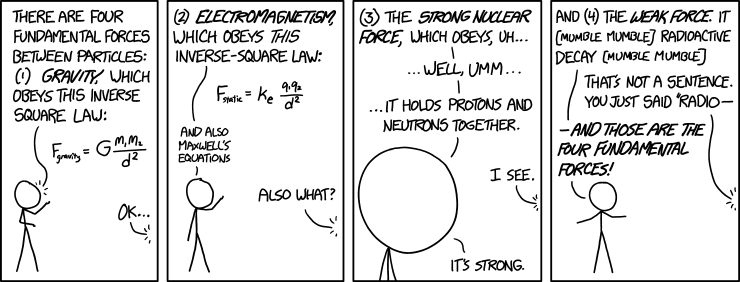
\includegraphics[width=12cm]{media/xkcd-fundamental-forces.png} \\[1em]
	\emph{Don't worry, I know what I'm doing!}
	\\ \scriptsize Image from \cite{img:xkcd}
\end{center}

There's also this thing called Zorn's lemma. It sounds terrifying,
because it's equivalent to the Axiom of Choice, which is also terrifying because why not.

In this post I will try to de-terrify these things,
because they're really not terrifying
and I'm not sure why no one bothered to explain this properly yet.
I have yet to see an olympiad handout that explains how you would construct
a pathological solution, even though it's really quite natural.
So let me fix this problem now\dots

\section{Let's construct a monster}
Let us just see if we can try and construct a ``bad'' $f$ and see what happens.

By scaling, let's assume WLOG that $f(1) = 1$.
Thus $f(n) = n$ for every integer $n$, and you can easily show from here that
\[ f\left( \frac mn \right) = \frac mn. \]
So $f$ is determined for all rationals. And then you get stuck.

None of this is useful for determining, say, $f(\sqrt 2)$.
You could add and subtract rational numbers all day
and, say, $\sqrt 2$ isn't going to show up at all.

Well, we're trying to set things on fire anyways, so let's set
\[ f(\sqrt 2) = 2015 \]
because why not?
By the same induction, we get $f(n\sqrt2) = 2015n$, and then that
\[ f\left( a + b \sqrt 2 \right) = a + 2015b. \]
Here $a$ and $b$ are rationals.
Well, so far so good -- as written, this is a perfectly good solution,
other than the fact that we've only defined $f$ on a tiny portion of the real numbers.

Well, we can do this all day:
\[ f\left( a + b \sqrt 2 + c \sqrt 3 + d \pi \right) = a + 2015b + 1337c - 999d. \]
Perfectly consistent.

You can kind of see how we should keep going now.
Just keep throwing in new real numbers which are ``independent''
to the previous few, assigning them to whatever junk we want.
It feels like it \emph{should} be workable. . .

In a moment I'll explain what ``independent'' means (though you
might be able to guess already), but at the moment there's a bigger issue:
no matter how many numbers we throw, it seems like we'll never finish.
Let's address the second issue first.

\section{Review of finite induction}
When you do induction, you get to count off $1$, $2$, $3$, \dots and so on.
So for example, suppose we had a ``problem'' such as:
\begin{quote}
	Prove that the intersection of $n$ open intervals is either $\varnothing$
	or an open interval.
\end{quote}
You can do this by induction easily: it's true for $n = 2$, and
for the larger cases it's similarly easy.

But you can't conclude from this that \emph{infinitely} many open intervals intersect
at some open interval. Indeed, this is false: consider the intervals
\[
	\left( -1, 1 \right), \quad
	\left( -\frac12, \frac12 \right), \quad
	\left( -\frac13, \frac13 \right), \quad
	\left( -\frac14, \frac14 \right), \quad
	\dots
\]
This \emph{infinite} set of intervals intersects at a single point $\{0\}$!

The moral of the story is that induction doesn't let us reach infinity.
Too bad, because we'd have loved to use induction to help us construct a monster.
That's what we're doing, after all -- adding things in one by one.

\section{Transfinite induction}
Well, it turns out we can, but we need a new notion of number,
the so-called \emph{ordinal number}.
I define these in their full glory in the first two sections of \Cref{ch:ordinal}
(and curious readers are even invited to jump ahead to those two sections),
but for this chapter I won't need that full definition yet.

Here's what I want to say: after all the natural numbers
\[ 0, \; 1, \; \dots, \]
I'll put a \emph{new number} called $\omega$,
the first ordinal greater than all the natural numbers.
After that there's more numbers called
\[\omega+1, \; \omega+2, \; \dots \]
and eventually a number called $2\omega$.

The list goes on:
\[
\begin{aligned}
	0, & 1, 2, 3, \dots, \omega \\
	& \omega+1, \omega+2, \dots, \omega+\omega \\
	& 2\omega+1, 2\omega+2, \dots, 3\omega \\
	& \vdots \\
	& \omega^2 + 1, \omega^2+2, \dots \\
	& \vdots \\
	& \omega^3, \dots, \omega^4, \dots, \omega^\omega
	\dots, \omega^{\omega^{\omega^{\dots}}} \\
\end{aligned}
\]
Pictorially, it kind of looks like this:
\begin{center}
	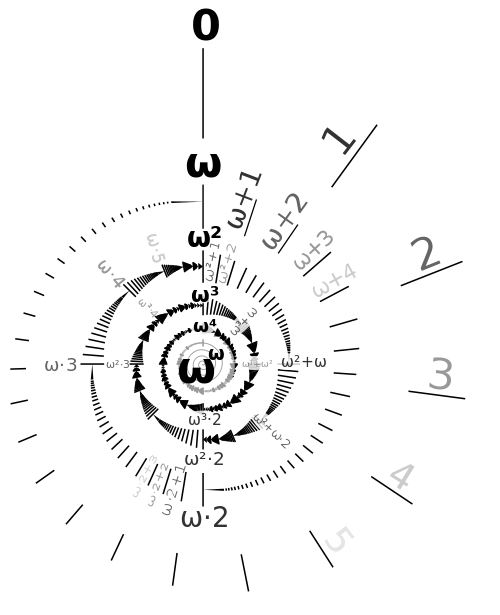
\includegraphics[scale=0.70]{media/500px-Omega-exp-omega-labeled.png}
	\\ \scriptsize Image from \cite{img:omega500}
\end{center}
(Note that the diagram only shows an initial segment;
there are still larger ordinals like $\omega^{\omega^{\omega}}+1000$ and so on).

Anyways, in the same way that natural numbers ``dominate'' all finite sets,
the ordinals dominate \emph{all the sets}, in the following sense.
Essentially, assuming the Axiom of Choice,
it follows that for every set $S$ there's some ordinal $\alpha$
which is larger than $S$ (in a sense I won't make precise until later chapters).

But it turns out (and you can intuitively see) that as large as the ordinals grow,
there is no \emph{infinite descending chain}.
Meaning: if I start at an ordinal (like $2 \omega + 4$) and jump down, I can only
take finitely many jumps before I hit $0$.
(To see this, try writing down a chain starting at $2 \omega + 4$ yourself.)
Hence, induction and recursion still work verbatim:
\begin{theorem}[Transfinite induction]
	Given a statement $P(-)$, suppose that
	\begin{itemize}
		\ii $P(0)$ is true, and
		\ii If $P(\alpha)$ is true for all $\alpha < \beta$, then $P(\beta)$ is true.
	\end{itemize}
	Then $P(\beta)$ is true.
\end{theorem}
Similarly, you're allowed to do recursion to define $x_\beta$ if you know the
value of $x_\alpha$ for all $\alpha < \beta$.

The difference from normal induction or recursion is that we'll often
only do things like ``define $x_{n+1} = \dots$''.
But this is not enough to define $x_\alpha$ for all $\alpha$.
To see this, try using our normal induction and see how far we can climb up the ladder.

Answer: you can't get $\omega$!
It's not of the form $n+1$ for any of our natural numbers $n$ -- our finite induction only lets us
get up to the ordinals less than $\omega$.
Similarly, the simple $+1$ doesn't let us hit the ordinal $2\omega$,
even if we already have $\omega+n$ for all $n$.
Such ordinals are called \vocab{limit ordinals}.
The ordinal that \emph{are} of the form $\alpha+1$ are called \vocab{successor ordinals}.

So a transfinite induction or recursion is very often broken up into three cases.
In the induction phrasing, it looks like
\begin{itemize}
	\ii (Zero Case) First, resolve $P(0)$.
	\ii (Successor Case) Show that from $P(\alpha)$ we can get $P(\alpha+1)$.
	\ii (Limit Case) Show that $P(\lambda)$ holds given $P(\alpha)$ for all $\alpha < \lambda$,
	where $\lambda$ is a limit ordinal.
\end{itemize}
Similarly, transfinite recursion often is split into cases too.
\begin{itemize}
	\ii (Zero Case) First, define $x_0$.
	\ii (Successor Case) Define $x_{\alpha+1}$ from $x_\alpha$.
	\ii (Limit Case) Define $x_\lambda$ from $x_\alpha$ for all $\alpha < \lambda$,
	where $\lambda$ is a limit ordinal.
\end{itemize}
In both situations, finite induction only does the first two cases,
but if we're able to do the third case we can climb far above the barrier $\omega$.

\section{Wrapping up functional equations}
Let's return to solving our problem.

Let $S_n$ denote the set of ``base'' numbers we have at the $n$th step.
In our example, we might have
\[
	S_1 = \left\{ 1 \right\}, \quad
	S_2 = \left\{ 1, \sqrt 2 \right\}, \quad
	S_3 = \left\{ 1, \sqrt 2, \sqrt 3 \right\}, \quad
	S_4 = \left\{ 1, \sqrt 2, \sqrt 3, \pi \right\}, \quad
	\dots
\]
and we'd like to keep building up $S_i$ until we can express all real numbers.
For completeness, let me declare $S_0 = \varnothing$.

First, I need to be more precise about ``independent''.
Intuitively, this construction is working because
\[ a + b \sqrt 2 + c \sqrt 3 + d \pi \]
is never going to equal zero for rational numbers $a$, $b$, $c$, $d$ (other than all zeros).
In general, a set $X$ of numbers is ``independent'' if the combination
\[ c_1 x_1 + c_2 x_2 + \dots + c_m x_m = 0 \]
never occurs for rational numbers $\QQ$ unless $c_1 = c_2 = \dots = c_m = 0$.
Here $x_i \in X$ are distinct. Note that even if $X$ is infinite,
I can only take finite sums!
(This notion has a name: we want $X$ to be \textbf{linearly independent} over $\QQ$;
see the chapter on vector spaces for more on this!)

When do we stop?
We'd like to stop when we have a set $S_{\text{something}}$ that's so big,
every real number can be written in terms of the independent numbers.
(This notion also has a name: it's called a $\QQ$-basis.)
Let's call such a set \textbf{spanning};
we stop once we hit a spanning set.

The idea that we can induct still seems okay:
suppose $S_\alpha$ isn't spanning.
Then there's some number that is independent of $S_\alpha$, say $\sqrt{2015}\pi$ or something.
Then we just add it to get $S_{\alpha+1}$.
And we keep going.

Unfortunately, as I said before it's not enough to be able to go from $S_\alpha$ to $S_{\alpha+1}$
(successor case); we need to handle the limit case as well.
But it turns out there's a trick we can do.
Suppose we've constructed \emph{all} the sets $S_0$, $S_1$, $S_2$, \dots, one for each positive integer $n$,
and none of them are spanning.
The next thing I want to construct is $S_\omega$; somehow I have to ``jump''.
To do this, I now take the infinite union
\[ S_\omega \overset{\text{def}}{=} S_0 \cup S_1 \cup S_2 \cup \dots. \]
The elements of this set are also independent (why?).

Ta-da!
With the simple trick of ``union all the existing sets'',
we've just jumped the hurdle to the first limit ordinal $\omega$.
Then we can construct $S_{\omega+1}$, $S_{\omega+2}$, \dots, once again --
just keep throwing in elements.
Then when we need to jump the next hurdle to $S_{2 \omega}$,
we just do the same trick of ``union-ing'' all the previous sets.

So we can formalize the process as follows:
\begin{enumerate}
	\ii Let $S_0 = \varnothing$.
	\ii For a successor stage $S_{\alpha+1}$, add any element to $S_\alpha$ to obtain $S_{\alpha+1}$.
	\ii For a limit stage $S_{\lambda}$, take the union $\bigcup_{\gamma < \lambda} S_\gamma$.
\end{enumerate}
How do we know that we'll stop eventually?
Well, the thing is that this process consumes a lot of real numbers.
In particular, the ordinals get larger than the size of $\RR$ (assuming Choice).
Hence if we don't stop we will quite literally reach a point where we have used up every single real number.
Clearly that's impossible, because by then the elements can't possibly be independent!

So by transfinite recursion, we eventually hit some $S_\gamma$ which is spanning:
the elements are all independent, but every real number can be expressed using it.
Done!

%Thus this problem is dead, dead, dead. Any questions?
%\begin{center}
%	\includegraphics[width=4cm]{media/squidzilla.png}
%\end{center}

\section{Zorn's lemma}
Now I can tell you what Zorn's lemma is:
it lets us do the same thing in any poset.

We can think of the above example as follows:
consider all sets of independent elements.
These form a partially ordered set by inclusion, and what we did
was quite literally climb up a chain
\[ S_0 \subsetneq S_1 \subsetneq S_2 \subsetneq \dots. \]
It's not quite climbing since we weren't just going one step at a time:
we had to do ``jumps'' to get up to $S_\omega$ and resume climbing.
But the main idea is to climb up a poset until we're at the very top;
in the previous case, when we reached the spanning set.

The same thing works verbatim with any \href{http://en.wikipedia.org/wiki/Partially_ordered_set}{partially ordered set}
$\mathcal P$.
Let's define some terminology.
A \vocab{local maximum} of the entire poset $\mathcal P$ is an element
which has no other elements strictly greater than it.
(Most authors refer to this as ``maximal element'', but I think
``local maximum'' is a more accurate term.)

Now a \vocab{chain of length $\gamma$} is a set of elements $p_\alpha$ for every $\alpha < \gamma$
such that $p_0 < p_1 < p_2 < \dots$.
(Observe that a chain has a last element if and only if $\gamma$ is a successor ordinal, like $\omega+3$.)
An \vocab{upper bound} to a chain is an element $\tilde p$ which is greater than or equal
to all elements of the chain;
In particular, if $\gamma$ is a successor ordinal, then just taking the last element of the chain works.

In this language, Zorn's lemma states that
\begin{theorem}
	[Zorn's lemma]
	Let $\mathcal P$ be a nonempty partially ordered set.
	If every chain has an upper bound,
	then $\mathcal P$ has a local maximum.
\end{theorem}

Chains with length equal to a successor ordinal always have upper bounds,
but this is not true in the limit case.
So the hypothesis of Zorn's lemma is exactly what
lets us ``jump'' up to define $p_\omega$ and other limit ordinals.
And the proof of Zorn's lemma is straightforward: keep climbing up the poset at successor stages,
using Zorn's condition to jump up at limit stages, and thus building a really long chain.
But we have to eventually stop, or we literally run out of elements of $\mathcal P$.
And the only possible stopping point is a local maximum.

If we want to phrase our previous solution in terms of Zorn's lemma, we'd say:
\begin{proof}
	Look at the poset whose elements are sets of independent real numbers.
	Every chain $S_0 \subsetneq S_1 \subsetneq \dots$ has an upper bound $\bigcup S_\alpha$
	(which you have to check is actually an element of the poset).
	Thus by Zorn, there is a local maximum $S$.
	Then $S$ must be spanning, because otherwise we could add an element to it.
\end{proof}
So really, Zorn's lemma is encoding all of the work of climbing that I argued earlier.
It's a neat little package that captures all the boilerplate, and tells
you exactly what you need to check.

\begin{center}
	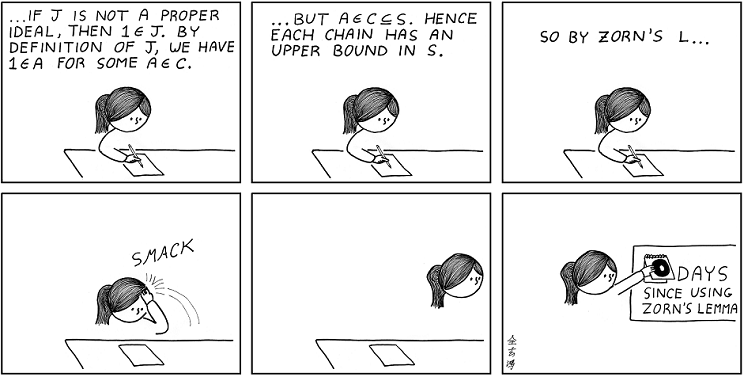
\includegraphics[scale=0.5]{media/zornaholic.png}
	\\ \scriptsize Image from \cite{img:zornaholic}
\end{center}

One last thing you might ask:
where is the Axiom of Choice used?
Well, the idea is that for any chain there could be lots of $\tilde p$'s,
and you need to pick one of them.
Since you are making arbitrary choices infinitely many times, you need the Axiom of Choice.
(Actually, you also need choice to talk about cardinalities as in theorem 1.)
But really, it's nothing special.

\section{\problemhead}
\begin{problem}
	[Tukey's lemma]
	Let $\mathcal F$ be a nonempty family of sets.
	Assume that for any set $A$,
	the set $A$ is in $\mathcal F$
	if and only if all its finite subsets are in $\mathcal F$.
	Prove that there exists $Y \in \mathcal F$
	such that $X \subseteq Y$ for every $X \in \mathcal F$.
\end{problem}

\chapter{Zermelo-Fraenkel with choice}
\label{ch:zfc}
Chapter $2\half$ of \cite{ref:msci} has a nice description of this.

\section{The ultimate functional equation}
In abstract mathematics, we often define structures by what \emph{properties}
they should have; for example, a group is a set and a binary operation
satisfying so-and-so axioms, while a metric space is a set and a distance function
satisfying so-and-so axioms.

Nevertheless, these definitions rely on previous definitions.
The colorful illustration of \cite{ref:msci} on this:
\begin{itemize}
	\ii A \emph{vector space} is an abelian group with\dots
	\ii An \emph{abelian group} has a binary operation such that\dots
	\ii A \emph{binary operation} on a set is\dots
	\ii A \emph{set} is \dots
\end{itemize}
and so on.

We have to stop at some point, because infinite lists of definitions are bad.
The stopping turns out to be a set, ``defined'' by properties.
The trick is that we never actually define what a set is,
but nonetheless postulate that these sets satisfy certain properties:
these are the $\ZFC$ axioms.
Loosely, $\ZFC$ can be thought of as the \emph{ultimate functional equation}.

Before talking about what these axioms are, I should talk about the caveats.

\section{Cantor's paradox}
Intuitively, a set is an unordered collection of elements.
Two sets are equal if they share the same elements:
\[
	\left\{ x \mid x \text{ is a featherless biped} \right\}
	=
	\left\{ x \mid x \text{ is human} \right\}
\]
(let's put aside the issue of dinosaurs).

As another example, we have our empty set $\varnothing$ that contains no objects.
We can have a set $\{1, 2, 3\}$, or maybe the set of natural numbers $\mathbb N = \{0, 1, 2, \dots \}$.
(For the purposes of set theory, $0$ is usually considered a natural number.)
Sets can even contain other sets, like $\left\{ \mathbb Z, \mathbb Q, \mathbb N \right\}$. Fine and dandy, right?

The trouble is that this definition actually isn't good enough, and here's why.
If we just say ``a set is any collection of objects'',
then we can consider a really big set $V$, the set of all sets.
So far no problem, right?
We would have the oddity that $V \in V$,
but oh well, no big deal.

Unfortunately, this existence of this $V$ leads immediately to a paradox.
The classical one is Bertrand's Paradox.
I will instead present a somewhat simpler one:
not only does $V$ contain itself, \emph{every subset $S \subseteq V$}
is itself an element of $V$ (i.e. $S \in V$).
If we let $\PP(V)$ denote the \vocab{power set} of $V$
(i.e.\ all the subsets of $V$), then we have an inclusion
\[ \PP(V) \injto V. \]
This is bad, since:
\begin{lemma}[Cantor's diagonal argument]
	\label{lem:cantor_diag}
	For \emph{any} set $X$, it's impossible to construct an injective
	map $\iota : \PP(X) \injto X$.
\end{lemma}
\begin{proof}
	Assume for contradiction $\iota$ exists.
	\begin{exercise}
		Show that if, $\iota$ exists,
		then there exists a surjective map $j : X \to \PP(X)$.
		(This is easier than it appears, just ``invert $\iota$'').
	\end{exercise}
	We now claim that $j$ can't exist.
	The idea is contained inside the picture:
	\[
		\begin{array}{cccccccc}
			&& x_1 & x_2 & x_3 & x_4 & x_5 & \dots \\ \cline{3-8}
			x_1 & \mapsto & \mathbf0 & 1 & 1 & 0 & 1 & \dots \\
			x_2 & \mapsto & 1 & \mathbf1 & 0 & 1 & 1 & \dots \\
			x_3 & \mapsto & 0 & 1 & \mathbf0 & 0 & 1 & \dots \\
			x_4 & \mapsto & 1 & 0 & 0 & \mathbf1 & 0 & \dots \\
			x_5 & \mapsto & 0 & 1 & 1 & 1 & \mathbf1 & \dots \\
			\vdots && \vdots & \vdots & \vdots & \vdots & \vdots & \ddots
		\end{array}
	\]
	here for each $j(x) \subseteq X$, I'm writing ``$1$'' to mean that
	the element is inside $j(x)$, and ``$0$'' otherwise.
	So $j(x_1) = \{x_2, x_3, x_5 \dots\}$.
	(Here the indices are ordinals rather than integers
	as $X$ may be uncountable.)

	Then we can read off the diagonal to get a new set.
	In our example, the diagonal specifies a set
	$A = \{x_2, x_4, x_5 \dots\}$.
	Then we invert it to get a set $B = \{x_1, x_3, \dots\}$.
	In symbols, we consider the set
	\[ B = \left\{ x \mid x \notin j(x) \right\} \]
	By construction, $B \subseteq X$ is not in the image of $j$,
	which is a contradiction since $j$ was supposed to be surjective.
\end{proof}

Now if you're not a set theorist, you could probably just brush this off,
saying ``oh well, I guess you can't look at certain sets''.
But if you're a set theorist, this worries you,
because you realize it means that you can't
just define a set as ``a collection of objects'',
because then everything would blow up.
Something more is necessary.

\section{The language of set theory}
We need a way to refer to sets other
than the informal description of ``collection of objects''.

So here's what we're going to do.
We'll start by defining a formal \emph{language of set theory},
a way of writing logical statements.
First of all we can throw in our usual logical operators:
\begin{itemize}
	\ii $\forall$ means ``for all''
	\ii $\exists$ means ``exists''
	\ii $=$ means ``equal''
	\ii $X \implies Y$ means ``if $X$ then $Y$''
	\ii $A \land B$ means ``$A$ and $B$''
	\ii $A \lor B$ means ``$A$ or $B$''
	\ii $\neg A$ means ``not $A$''.
\end{itemize}

Since we're doing set theory,
there's only one more operator we add in: the inclusion $\in$.
And that's all we're going to use (for now).

So how do we express something like ``the set $\{1, 2\}$''?
The trick is that we're not going to actually ``construct'' any sets,
but rather refer to them indirectly, like so:
\[ \exists S : x \in S \iff \left( (x=1) \lor (x=2) \right). \]
This reads: ``there exists an $S$ such that $x$ is in $S$ if
and only if either $x=1$ or $x=2$''.
We don't have to refer to sets as objects in and of
themselves anymore --- we now have a way to ``create'' our sets,
by writing formulas for exactly what they contain.
This is something a machine can parse.

Well, what are we going to do with things like $1$ and $2$, which are not sets?
Answer:
\begin{moral}
	Elements of sets are themselves sets.
\end{moral}
We're going to make \textbf{everything} into a set.
Natural numbers will be sets. Ordered pairs will be sets. Functions will be sets.
Later, I'll tell you exactly how we manage to do something like encode $1$ as a set.
For now, all you need to know is that that sets don't just hold objects;
they hold other sets.

So now it makes sense to talk about whether something is a set or not:
$\exists x$ means ``$x$ is a set'', while $\nexists x$ means ``$x$ is not a set''.
In other words, we've rephrased the problem of deciding whether something
is a set to whether it exists,
which makes it easier to deal with in our formal language.
That means that our axiom system had better find some way to let us
show a lot of things exist, without letting us prove
\[ \exists S \forall x : x \in S. \]
For if we prove this formula,
then we have our ``bad'' set that caused us to go down the
rabbit hole in the first place.

\section{The axioms of $\ZFC$}
I don't especially want to get into details about these axioms;
if you're interested, read:
\begin{itemize}
	\ii \footnotesize \url{https://usamo.wordpress.com/2014/11/13/set-theory-an-intro-to-zfc-part-1/}
	\ii \footnotesize \url{https://usamo.wordpress.com/2014/11/18/set-theory-part-2-constructing-the-ordinals/}
\end{itemize}
Here is a much terser description of the axioms,
which also includes the corresponding sentence in the language of set theory.
It is worth the time to get some practice parsing $\forall$, $\exists$, etc.\
and you can do so by comparing the formal sentences with the natural statement of the axiom.

First, the two easiest axioms:
\begin{itemize}
	\ii $\Extensionality$ is the sentence
	$\forall x \forall y
	\left( \left( \forall a  \left( a \in x \iff a \in y \right) \right)
	\implies x = y \right)$,
	which says that if two sets $x$ and $y$ have the same elements,
	then $x = y$.

	\ii $\EmptySet$ is the sentence $\exists a : \forall x \; \neg (x \in a)$;
	it says there exists a set with no elements.
	By $\Extensionality$ this set is unique, so we denote it $\varnothing$.
\end{itemize}

The next two axioms give us basic ways of building new sets.
\begin{itemize}
	\ii Given two elements $x$ and $y$, there exists a set $a$ containing only those two elements.
	In machine code, this is the sentence $\Pairing$, written
	\[ \forall x \forall y \exists a \quad \forall z,
		\; z \in a \iff \left( (z=x) \lor (z=y) \right). \]
	By $\Extensionality$ this set $a$ is unique, so we write $a = \{x,y\}$.

	\ii Given a set $a$, we can create the union of the elements of $a$.
	For example, if $a = \{ \{1,2\}, \{3,4\} \}$, then $U = \{1,2,3,4\}$ is a set.
	Formally, this is the sentence $\Union$:
	\[ \forall a \exists U \quad \forall x \;
		\left[ (x \in U) \iff (\exists y : x \in y \in a) \right]. \]
	Since $U$ is unique by $\Extensionality$, we denote it $\cup a$.

	\ii 
	We can construct the \vocab{power set} $\mathcal P(x)$.
	Formally, the sentence $\PowerSet$ says that
	\[ \forall x \exists P \forall y (y \in P \iff y \subseteq x) \]
	where $y \subseteq x$ is short for $\forall z (z \in y \implies z \in x)$.
	As $\Extensionality$ gives us uniqueness of $P$,
	we denote it $\mathcal P(x)$.

	\ii $\Foundation$ says there are no infinite descending chains
	\[ x_0 \ni x_1 \ni x_2 \ni \dots. \]
	This is important, because it lets us induct.
	In particular, \textbf{no set contains itself}.

	\ii $\Infinity$ implies that $\omega = \{0,1,\dots\}$ is a set.
\end{itemize}
These are all things you are already used to, so keep your intuition there.
The next one is less intuitive:
\begin{itemize}
	\ii The \vocab{schema of restricted comprehension} says:
	if we are \emph{given a set $X$}, and some formula $\phi(x)$
	then we can \emph{filter} through the elements of $X$ to get a subset
	\[ Y = \left\{ x \in X \mid \phi(x) \right\}. \]
	% (For example $\phi(x)$ might be ``$x$ is not the empty set, i.e. $\exists a(a\in x)$'')
	Formally, given a formula $\phi$:
	\[
		\forall X \quad \exists Y \quad
		\forall y (y \in Y \iff y \in X \land \phi(y)).
	\]
\end{itemize}
Notice that we may \emph{only} do this filtering over an already given set.
So it is not valid to create
$ \left\{ x \mid x \text{ is a set} \right\} $.
We are thankful for this, because this lets us evade Cantor's paradox.

\begin{abuse}
	Note that technically, there are infinitely many sentences,
	a $\Comprehension_\phi$ for every possible formula $\phi$.
	By abuse of notation, we let $\Comprehension$ abbreviate
	the infinitely many axioms $\Comprehension_\phi$ for every $\phi$.
\end{abuse}

There is one last schema called $\Replacement_\phi$.
Suppose $X$ is a set and $\phi(x,y)$ is some formula
such that for every $x \in X$, there is a \emph{unique} $y$ in the universe
such that $\phi(x,y)$ is true: for example ``$y = x \cup \{x\}$'' works.
(In effect, $\phi$ is defining a function $f$ on $X$.)
Then there exists a set $Y$ consisting exactly of these images:
(i.e. $f``X$ is a set).
\begin{abuse}
	By abuse of notation, we let $\Replacement$ abbreviate
	the infinitely many axioms $\Replacement_\phi$ for every $\phi$.
\end{abuse}

We postpone discussion of the Axiom of Choice momentarily.

\section{Encoding}
Now that we have this rickety universe of sets, we can start re-building math.
You'll get to see this more in the next chapter on ordinal numbers.

\begin{definition}
	An \vocab{ordered pair} $(x,y)$
	is a set of the form
	\[ (x,y) \defeq 
		\left\{ \left\{ x \right\}, \left\{ x,y \right\} \right\}. \]
\end{definition}
Note that $(x,y) = (a,b)$ if and only if $x=a$ and $y=b$.
Ordered $k$-tuples can be defined recursively: a three-tuple $(a,b,c)$ means $(a,(b,c))$.

\begin{definition}
	A \vocab{function} $f : X \to Y$
	is defined as a collection of ordered pairs such that
	\begin{itemize}
		\ii If $(x,y) \in f$, then $x \in X$ and $y \in Y$.
		\ii For every $x \in X$, there is a unique $y \in Y$
		such that $(x,y) \in f$. We denote this $y$ by $f(x)$.
	\end{itemize}
\end{definition}

\begin{definition}
	The \vocab{natural numbers} are defined inductively as
	\begin{align*}
		0 &= \varnothing \\
		1 &= \{0\} \\
		2 &= \{0,1\} \\
		3 &= \{0,1,2\} \\
		&\vdotswithin=
	\end{align*}
	The set of all natural numbers is denoted $\omega$.
\end{definition}
\begin{abuse}
	Yes, I'm sorry, in set theory $0$ is considered a natural number.
	For this reason I'm using $\omega$ and not $\NN$
	since I explicitly have $0\notin\NN$ in all other parts of this book.
\end{abuse}

Et cetera, et cetera.

\section{Choice and well-ordering}
The Axiom of Choice states that given a collection $Y$ of nonempty sets,
there is a function $g : Y \to \cup Y$ which ``picks'' an element of each member of $Y$.
That means $g(y) \in y$ for every $y \in Y$.
(The typical illustration is that $Y$ contains infinitely many drawers,
and each drawer (a $y$) has some sock in it.)

Formally, it is the sentence
\[ \forall Y \left(\varnothing \notin Y
	\implies 
	\exists g : Y \to \cup Y
	\text{ such that }
	\forall y \in Y \left( g(y) \in y \right).
	\right)
\]
The tricky part is not that we can conceive of such a function $g$,
but that in fact this function $g$ is \emph{actually a set}.

There is an equivalent formulation which is often useful.
\begin{definition}
	A \vocab{well-ordering} $<$ of $X$ is a strict, total order on $X$
	which has no infinite descending chains.
\end{definition}
Well-orderings on a set are very nice, because we can pick minimal elements:
this lets us do induction, for example.
\begin{example}[Examples and non-examples of well-orderings]
	\listhack
	\begin{enumerate}[(a)]
		\ii The natural numbers $\omega = \{0,1,2,\dots\}$
		are well-ordered by $<$.
		\ii The integers $\ZZ = \{\dots,-2,-1,0,1,2,\dots\}$ are not well-ordered by $<$,
		because there are infinite descending chains (take $-1 > -2 > -3 > \dots$).
		\ii The positive real numbers are not well-ordered by $<$,
		again because of the descending chain $\frac11>\frac12>\frac13>\dots$.
		\ii The positive integers are not well-ordered by the divisibility operation $\mid$.
		While there are no descending chains, there are elements which cannot be compared
		(for example $3 \nmid 5$, $5 \nmid 3$ and $3 \neq 5$).
	\end{enumerate}
\end{example}

\begin{theorem}
	[Well-ordering theorem]
	Assuming Choice, for every set we can place some well-ordering on it.
\end{theorem}
In fact, the well-ordering theorem is actually equivalent to the axiom of choice.

\section{Sets vs classes}
\prototype{The set of all sets is the standard example of a proper class.}
We close the discussion of $\ZFC$ by mentioning ``classes''.

Roughly, the ``bad thing'' that happened was that we considered a set $S$, the
``set of all sets'', and it was \emph{too big}.
That is,
\[ \left\{ x \mid x \text{ is a set} \right\} \]
is not good.
Similarly, we cannot construct a set
\[ \left\{ x \mid x \text{ is an ordered pair} \right\}. \]
The lesson of Cantor's Paradox is that we cannot create any sets we want;
we have to be more careful than that.

Nonetheless, if we are given a set
we can still tell whether or not it is an ordered pair.
So for convenience, we will define a \vocab{class} to be
a ``concept'' like the ``class of all ordered pairs''.
Formally, a class is defined by some formula $\phi$:
it consists of the sets which satisfy the formula.

In particular:
\begin{definition}
	The class of all sets is denoted $V$, defined by $V = \left\{ x \mid x=x \right\}$.
	It is called the \vocab{von Neumann universe}.
\end{definition}

A class is a \vocab{proper class} if it is not a set,
so for example we have:
\begin{theorem}[There is no set of all sets]
	$V$ is a proper class.
\end{theorem}
\begin{proof}
	Assume not, and $V$ is a set. Then $V \in V$,
	which violates $\Foundation$.
	(In fact, $V$ cannot be a set even without $\Foundation$,
	as we saw earlier).
\end{proof}

\begin{abuse}
	Given a class $C$, we will write $x \in C$ to mean
	that $x$ has the defining property of $C$.
	For example, $x \in V$ means ``$x$ is a set''.

	It does not mean $x$ is an element of $V$
	-- this doesn't make sense as $V$ is not a set.
\end{abuse}

\section\problemhead
\begin{problem}
	Let $A$ and $B$ be sets.
	Show that $A \cap B$ and $A \times B$ are sets.
\end{problem}

\begin{problem}
	Show that the class of all groups is a proper class.
	(You can take the definition of a group as a pair $(G, \cdot)$
	where $\cdot$ is a function $G \times G \to G$.)
\end{problem}
\begin{problem}
	Show that the axiom of choice follows from the well-ordering theorem.
\end{problem}

\begin{dproblem}
	Prove that actually, $\Replacement \implies \Comprehension$.
\end{dproblem}

\begin{problem}
	[From Taiwan IMO training camp]
	Consider infinitely many people each wearing a hat,
	which is either red, green, or blue.
	Each person can see the hat color of everyone except themselves.
	Simultaneously each person guesses the color of their hat.
	Show that they can form a strategy such that at most finitely many people guess their color incorrectly. 
\end{problem}

\chapter{Ordinals}
\section{Counting for preschoolers}
In preschoolers, we were told to count as follows.
We defined a set of symbols $1$, $2$, $3$, $4$, \dots.
Then the teacher would hold up three apples and say:
\begin{quote}
	``One . . . two . . . three!  There are three apples.''
\end{quote}

\begin{center}
	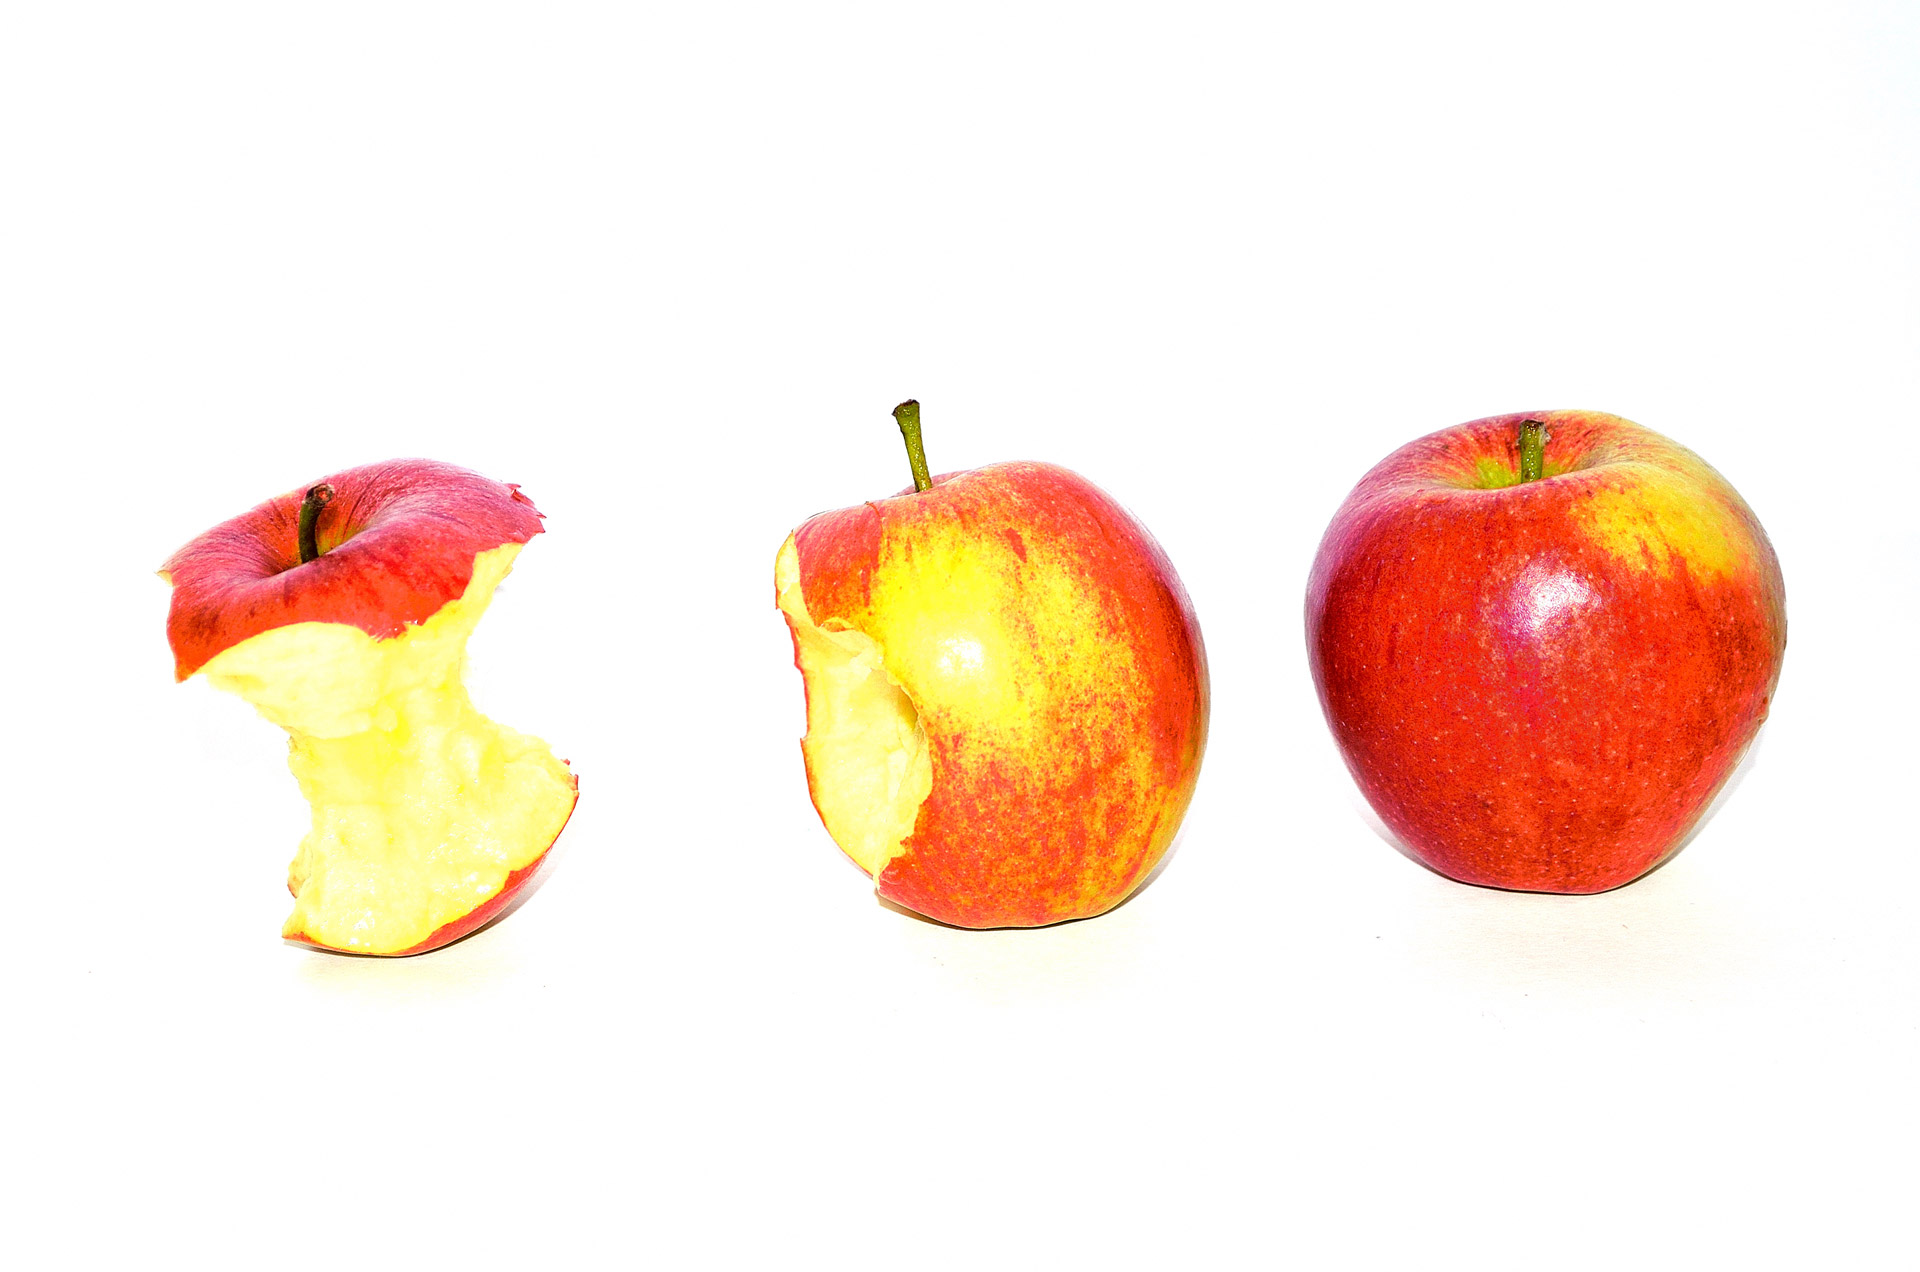
\includegraphics[height=5cm]{media/three-apples.jpg}
\end{center}


The implicit definition is that the \emph{last} number said is the final answer.
This raises some obvious problems if we try to count infinite sets,
but even in the finite world,
this method of counting fails for the simplest set of all:
how many apples are in the following picture?

\begin{center}
	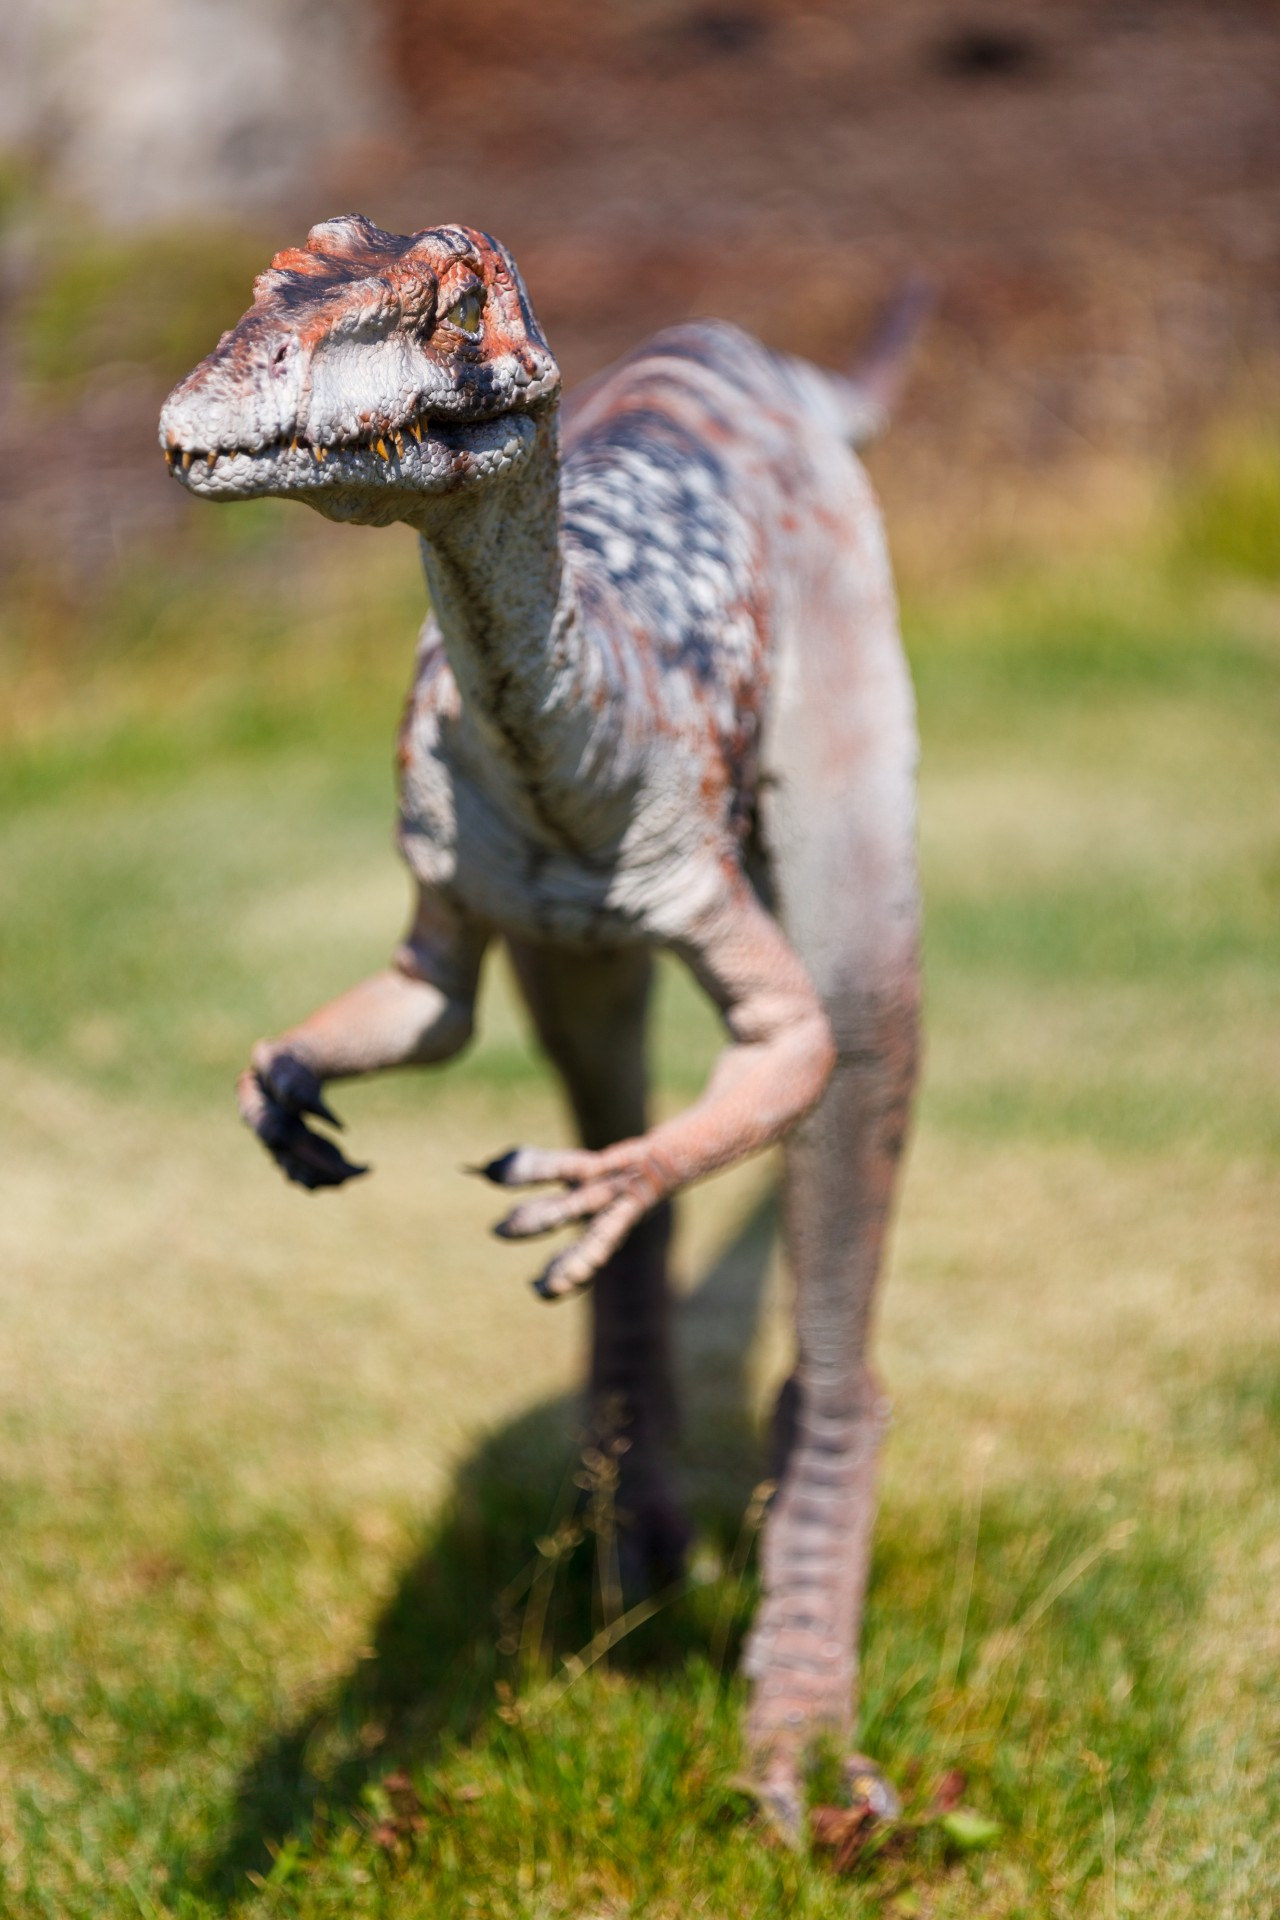
\includegraphics[height=5cm]{media/velociraptor.jpg}
\end{center}

Answer: $0$. There is nothing to say, and our method of counting has failed
for the simplest set of all: the empty set.

\section{Counting for set theorists}
\prototype{$\omega+1 = \{0,1,2,\dots,\omega\}$ might work.}
Rather than using the \emph{last} number listed, I propose the following:
we start with a list of symbols $0$, $1$, $2$, \dots\ and our final answer
is going to be the \emph{first} number which was \emph{not} said.
Thus to count three apples, we would say 
\begin{quote}
	``Zero . . . one . . . two!  There are three apples.''
\end{quote}
We will call these numbers \emph{ordinal numbers} (rigorous definition later).
In particular, we'll \emph{define} each ordinal to be the set of things we say:
\begin{align*}
	0 &= \varnothing \\
	1 &= \{0\} \\
	2 &= \{0,1\} \\
	3 &= \{0,1,2\} \\
	&\vdotswithin=
\end{align*}
In this way we can write out the natural numbers.
You can have some fun with this, by saying things like
\[
	4 \defeq
	\left\{ 
		\left\{  \right\},
		\left\{ \left\{  \right\} \right\},
		\left\{ \left\{  \right\}, \left\{ \left\{  \right\} \right\} \right\},
		\left\{ 
			\left\{  \right\},
			\left\{ \left\{  \right\} \right\},
			\left\{ \left\{  \right\}, \left\{ \left\{  \right\} \right\} \right\}
		\right\}
	\right\}
\]
In this way, we soon write down all the natural numbers.
The next ordinal, $\omega$,\footnote{
	That $\omega$ is actually a set is not obvious.
	The proof follows from the actual statement of $\Infinity$,
	which I've dutifully omitted.
	In fact, $\Infinity$ is equivalent to the existence of $\omega$.
} is defined as
\begin{align*}
	\omega &= \left\{ 0, 1, 2, \dots \right\} \\
	\intertext{Then comes}
	\omega+1 &= \left\{ 0, 1, 2, \dots, \omega \right\} \\
	\omega+2 &= \left\{ 0, 1, 2, \dots, \omega, \omega+1 \right\} \\
	\omega+3 &= \left\{ 0, 1, 2, \dots, \omega, \omega+1, \omega+2 \right\} \\
	&\vdotswithin= \\
	\intertext{And in this way we define $\omega+n$, and eventually reach}
	\omega \cdot 2 = \omega+\omega &= \left\{ 0, 1, 2 \dots, \omega, \omega+1, \omega+2, \dots \right\} \\
	\omega \cdot 2 + 1 &= \left\{ 0, 1, 2 \dots, \omega, \omega+1, \omega+2, \dots, \omega \cdot 2 \right\}.
\end{align*}
In this way we obtain
\begin{align*}
	0,\; & 1,\; 2,\; 3,\; \dots,\; \omega \\
	& \omega+1,\; \omega+2,\; \dots,\; \omega+\omega \\
	& \omega \cdot 2 +1,\; \omega \cdot 2 +2,\; \dots,\; \omega \cdot 3,\; \\
	& \vdots \\
	& \omega^2 + 1,\; \omega^2+2,\; \dots \\
	& \vdots \\
	& \omega^3,\; \dots,\; \omega^4,\; \dots,\; \omega^\omega \\
	& \vdots \\
	& \omega^{\omega^{\omega^{\dots}}} \\
\end{align*}

The first several ordinals can be illustrated in the following nice spiral.
\begin{center}
	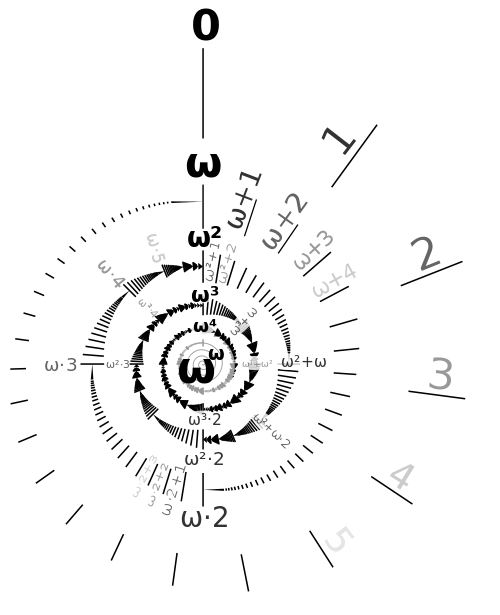
\includegraphics[scale=0.60]{media/500px-Omega-exp-omega-labeled.png}
\end{center}


\begin{remark}
	(Digression)
	The number $\omega^{\omega^{\omega^{\dots}}}$ has a name, $\eps_0$;
	it has the property that $\omega^{\eps_0} = \omega$.
	The reason for using ``$\eps$'' (which is usually used to denote small quantities)
	is that, despite how huge it may appear, it is actually a countable set.
	More on that later.
\end{remark}

\section{Definition of an ordinal}
Our informal description of ordinals gives us a chain
\[ 0 \in 1 \in 2 \in \dots \in \omega \in \omega+1 \in \dots. \]
To give the actual definition of an ordinal, I need to define two auxiliary terms first.
\begin{definition}
	A set $x$ is \vocab{transitive} if whenever $z \in y \in x$, we have $z \in x$ also.
\end{definition}
\begin{example}
	[$7$ is transitive]
	The set $7$ is transitive: for example, $2 \in 5 \in 7 \implies 2 \in 7$.
\end{example}
\begin{ques}
	Show that this is equivalent to: whenever $y \in x$, $y \subseteq x$.
\end{ques}
Moreover, recall the definition of ``well-ordering'': a strict linear order
with no infinite descending chains.
\begin{example}
	[$\in$ is a well-ordering on $\omega \cdot 3$]
	In $\omega \cdot 3$, we have an ordering
	\[ 0 \in 1 \in 2 \in \dots \in \omega \in \omega+1 \in \dots
		\in \omega \cdot 2 \in \omega \cdot 2 + 1 \in \dots. \]
	which has no infinite descending chains.
	Indeed, a typical descending chain might look like
	\[ \omega \cdot 2 + 6 \ni \omega \cdot 2 \ni
		\omega + 2015 \ni \omega+3 \ni \omega \ni 1000 \ni 256 \ni 42 \ni 7 \ni 0. \]
	Even though there are infinitely many elements, there is no way
	to make an infinite descending chain.
\end{example}
\begin{exercise}
	(Important) Convince yourself there are no infinite descending chains of ordinals at all
	(which must be true by $\Foundation$!).
\end{exercise}

\begin{definition}
	An \vocab{ordinal} is a transitive set which is well-ordered by $\in$.
	The class of all ordinals is denoted $\On$.
\end{definition}

\begin{ques}
	Satisfy yourself that this definition works.
\end{ques}

We typically use Greek letters $\alpha$, $\beta$, etc.\ for ordinal numbers.
\begin{definition}
	We write
	\begin{itemize}
		\ii $\alpha < \beta$ to mean $\alpha \in \beta$,
		and $\alpha > \beta$ to mean $\alpha \ni \beta$.
		\ii $\alpha \le \beta$ to mean $\alpha \in \beta$ or $\alpha = \beta$,
		and $\alpha \ge \beta$ to mean $\alpha \ni \beta$ or $\alpha = \beta$,
	\end{itemize}
\end{definition}

\begin{theorem}[Ordinals are strictly ordered]
	Given any two ordinal numbers $\alpha$ and $\beta$,
	either $\alpha < \beta$, $\alpha = \beta$ or $\alpha > \beta$.
\end{theorem}
\begin{proof}
	Surprisingly annoying, thus omitted.
\end{proof}
\begin{theorem}[Ordinals represent all order types]
	Suppose $<$ is a well-ordering on a set $X$.
	Then there exists a unique ordinal $\alpha$
	such that there is a bijection $\alpha \to X$
	which is order preserving.
\end{theorem}
Thus ordinals represent the possible \emph{equivalence classes} of order types.
Any time you have a well-ordered set, it is isomorphic to a unique ordinal.

We now formalize the ``$+1$'' operation we were doing:
\begin{definition}
	Given an ordinal $\alpha$, we let $\alpha+1 = \alpha \cup \{\alpha\}$.
	An ordinal of the form $\alpha+1$ is called a \vocab{successor ordinal}.
\end{definition}
\begin{definition}
	If $\lambda$ is an ordinal which is neither zero nor a successor ordinal,
	then we say $\lambda$ is a \vocab{limit ordinal}.
\end{definition}
\begin{example}
	[Sucessor and limit ordinals]
	$7$, $\omega+3$, $\omega\cdot2+2015$ are successor ordinals,
	but $\omega$ and $\omega \cdot 2$ are limit ordinals.
\end{example}

\section{Ordinals are ``tall''}
First, we note that:
\begin{theorem}
	[There is no set of all ordinals]
	$\On$ is a proper class.
\end{theorem}
\begin{proof}
	Assume for contradiction not.
	Then $\On$ is well-ordered by $\in$ and transitive, so $\On$ is an ordinal,
	i.e.\ $\On \in \On$, which violates $\Foundation$.
\end{proof}

\begin{figure}[ht]
	\centering
	\snsd[width=0.5\textwidth]{ordinals.jpg}
	\caption{What happens when people do not follow first-order logic.}
\end{figure}


From this we deduce:
\begin{theorem}
	[Sets of ordinals are bounded]
	Let $A \subseteq \On$.
	Then there is some ordinal $\alpha$ such that $A \in \alpha$
	(i.e.\ $A$ must be bounded).
\end{theorem}
\begin{proof}
	Otherwise, look at $\cup A$.
	It is a set.
	But if $A$ is unbounded it must equal $\On$,
	which is a contradiction.
\end{proof}
In light of this, every set of ordinals has a \vocab{supremum},
which is the least upper bound. We denote this by $\sup A$.

\begin{ques}
	Show that
	\begin{enumerate}[(a)]
		\ii $\sup (\alpha+1) = \alpha$ for any ordinal $\alpha$.
		\ii $\sup \lambda = \lambda$ for any limit ordinal $\lambda$.
	\end{enumerate}
\end{ques}

The pictorial ``tall'' will be explained in a few sections.

\section{Transfinite induction and recursion}
The fact that $\in$ has no infinite descending chains means that induction and recursion still work verbatim.
\begin{theorem}[Transfinite induction]
	Given a statement $P(-)$, suppose that
	\begin{itemize}
		\ii $P(0)$ is true, and
		\ii If $P(\alpha)$ is true for all $\alpha < \beta$, then $P(\beta)$ is true.
	\end{itemize}
	Then $P(\alpha)$ is true for every ordinal $\alpha$.
\end{theorem}
\begin{theorem}
	[Transfinite recursion]
	To define a sequence $x_\alpha$ for every ordinal $\alpha$,
	it suffices to
	\begin{itemize}
		\ii define $x_0$, then
		\ii for any $\beta$, define $x_\beta$ for any $\alpha < \beta$.
	\end{itemize}
\end{theorem}

The difference between this and normal induction lies in the \emph{limit ordinals}.
In real life, we might only do things like ``define $x_{n+1} = \dots$''.
But this is not enough to define $x_\alpha$ for all $\alpha$,
because we can't hit $\omega$ this way.
Similarly, the simple $+1$ doesn't let us hit the ordinal $2\omega$,
even if we already have $\omega+n$ for all $n$.
In other words, simply incrementing by $1$ cannot get us past limit stages,
but using transfinite induction to jump upwards lets us sidestep this issue.

So a transfinite induction or recursion is very often broken up into three cases.
In the induction phrasing, it looks like
\begin{itemize}
	\ii (Zero Case) First, resolve $P(0)$.
	\ii (Successor Case) Show that from $P(\alpha)$ we can get $P(\alpha+1)$.
	\ii (Limit Case) For $\lambda$ a limit ordinal,
	show that $P(\lambda)$ holds given $P(\alpha)$ for all $\alpha < \lambda$,
	where $\lambda$ is a limit ordinal.
\end{itemize}
Similarly, transfinite recursion often is split into cases too.
\begin{itemize}
	\ii (Zero Case) First, define $x_0$.
	\ii (Successor Case) Define $x_{\alpha+1}$ from $x_\alpha$.
	\ii (Limit Case) Define $x_\lambda$ from $x_\alpha$ for all $\alpha < \lambda$,
	where $\lambda$ is a limit ordinal.
\end{itemize}
In both situations, finite induction only does the first two cases,
but if we're able to do the third case we can climb above the barrier $\omega$.

\section{Ordinal arithmetic}
\prototype{$1+\omega=\omega \neq \omega+1$.}
To give an example of transfinite recursion, let's define addition of ordinals.
Recall that we defined $\alpha+1 = \alpha \cup \{\alpha\}$.
By transfinite recursion, let
\begin{align*}
	\alpha + 0 &= \alpha \\
	\alpha + (\beta + 1) &= (\alpha + \beta) + 1 \\
	\alpha + \lambda &= \bigcup_{\beta < \lambda} (\alpha + \beta).
\end{align*}
Here $\lambda \neq 0$.

We can also do this explicitly:
The picture is to just line up $\alpha$ after $\beta$.
That is, we can consider the set
\[
	X = 
	\left( \left\{ 0 \right\} \times \alpha \right)
	\cup
	\left( \left\{ 1 \right\} \times \beta \right)
\]
(i.e.\ we tag each element of $\alpha$ with a $0$, and
each element of $\beta$ with a $1$).
We then impose a well-ordering on $X$ by a lexicographic ordering $\llex$
(sort by first component, then by second).
This well-ordering is isomorphic to a unique ordinal, 
\begin{example}
	[$2+3=5$]
	Under the explicit construction for $\alpha = 2$ and $\beta = 3$, we get the set
	\[
		X = \left\{ (0,0) < (0,1) < (1,0) < (1,1) < (1,2) \right\}
	\]
	which is isomorphic to $5$.
\end{example}

\begin{example}[Ordinal arithmetic is not commutative]
	Note that $1 + \omega = \omega$!
	Indeed, under the transfinite definition, we have
	\[ 1 + \omega = \cup_n (1+n) = 2 \cup 3 \cup 4 \cup \dots = \omega. \]
	With the explicit construction, we have
	\[ X = \left\{ (0,0) < (1,0) < (1,1) < (1,2) < \dots \right\} \]
	which is isomorphic to $\omega$.
\end{example}
\begin{exercise}
	Show that $n+\omega = \omega$ for any $n \in \omega$.
\end{exercise}

\begin{remark}
	Ordinal addition is not commutative.
	However, from the explicit construction
	we can see that it is at least associative.
\end{remark}

Similarly, we can define multiplication in two ways.
By transfinite induction:
\begin{align*}
	\alpha \cdot 0 &= 0 \\
	\alpha \cdot (\beta + 1) &= (\alpha \cdot \beta) + \alpha \\
	\alpha \cdot \lambda &= \bigcup_{\beta < \lambda} \alpha \cdot \beta.
\end{align*}
We can also do an explicit construction: $\alpha \cdot \beta$
is the order type of
\[ \llex \text{ applied to } \beta \times \alpha. \]
\begin{example}[Ordinal multiplication is not commutative]
	We have $\omega \cdot 2 = \omega + \omega$,
	but $2 \cdot \omega = \omega$.
\end{example}
\begin{exercise}
	Prove this.
\end{exercise}
\begin{exercise}
	Verify that ordinal multiplication
	(like addition) is associative but not commutative.
	(Look at $\gamma \times \beta \times \alpha$.)
\end{exercise}

Exponentiation can also be so defined, though the explicit construction is less natural.
\begin{align*}
	\alpha^0 &= 1 \\
	\alpha^{\beta+1} &= \alpha^{\beta} \cdot \alpha \\
	\alpha^{\lambda} &= \bigcup_{\beta < \lambda} \alpha^\beta.
\end{align*}
\begin{exercise}
	Verify that $2^\omega = \omega$.
\end{exercise}


\section{The hierarchy of sets}
We now define the \vocab{von Neumann Hierarchy} by transfinite recursion.
\begin{definition}
	By transfinite recursion, we set
	\begin{align*}
		V_0 &= \varnothing \\
		V_{\alpha + 1} &= \PP(V_\alpha) \\
		V_\lambda &= \bigcup_{\alpha<\lambda} V_\alpha
	\end{align*}
\end{definition}
By transfinite induction, we see $V_\alpha$ is transitive
and that $V_\alpha \subseteq V_\beta$ for all $\alpha < \beta$.

\begin{example}[$V_\alpha$ for $\alpha \le 3$]
	The first few levels of the hierarchy are:
	\begin{align*}
		V_0 &= \varnothing \\
		V_1 &= \left\{ 0 \right\} \\
		V_2 &=  \left\{ 0, 1 \right\} \\
		V_3 &= \left\{ 0, 1, 2, \left\{ 1 \right\} \right\}.
	\end{align*}
	Notice that for each $n$, $V_n$ consists of only finite sets,
	and each $n$ appears in $V_{n+1}$ for the first time.
	Observe that
	\[ V_\omega = \bigcup_{n \in \omega} V_n \]
	consists only of finite sets; thus $\omega$ appears for the first time
	in $V_{\omega+1}$.
\end{example}
\begin{ques}
	How many sets are in $V_5$?
\end{ques}

\begin{definition}
	The \vocab{rank} of a set $y$, denoted $\rank(y)$,
	is the smallest ordinal $\alpha$ such that $y \in V_{\alpha+1}$.
\end{definition}
\begin{example}
	$\rank(2) = 2$, and actually $\rank(\alpha)=\alpha$
	for any ordinal $\alpha$ (problem later).
	This is the reason for the extra ``$+1$''.
\end{example}
\begin{ques}
	Show that $\rank(y)$ is the smallest ordinal $\alpha$
	such that $y \subseteq V_\alpha$.
\end{ques}

It's not yet clear that the rank of a set actually exists, so we prove:
\begin{theorem}[The von Neumann hierachy is complete]
	The class $V$ is equal to $\bigcup_{\alpha \in \On} V_\alpha$.
	In other words, every set appears in some $V_\alpha$.
\end{theorem}
\begin{proof}
	Assume for contradiction this is false.
	The key is that because $\in$ satisfies $\Foundation$,
	we can take a $\in$-minimal counterexample $x$.
	Thus $\rank(y)$ is defined for every $y \in x$,
	and we can consider (by $\Replacement$) the set
	\[ \left\{ \rank(y) \mid y \in x \right\}. \]
	Since it is a set of ordinals, it is bounded.
	So there is some large ordinal $\alpha$ such that $y \in V_\alpha$
	for all $y \in x$, i.e.\ $x \subseteq V_\alpha$,
	so $x \in V_{\alpha+1}$.
\end{proof}

This leads us to the following picture of the universe $V$.

\begin{center}
	\begin{asy}
		size(11cm);
		pair A = (12,30);
		pair B = -conj(A);
		pair M = midpoint(A--B);
		pair O = origin;
		MP("V", A, dir(10));
		draw(A--O--B);

		fill(A--O--B--cycle, opacity(0.3)+palecyan);

		MP("V_0 = \varnothing", origin, dir(-20));
		MP("V_1 = \{\varnothing\}", 0.05*A, dir(0));
		MP("V_2 = \{\varnothing, \{\varnothing\} \}", 0.10*A, dir(0));

		draw(MP("V_n", 0.3*A, dir(0))--0.3*B);
		draw(MP("V_{n+1} = \mathcal P(V_n)", 0.35*A, dir(0))--0.35*B);
		Drawing("n", 0.35*M, dir(45));

		draw(MP("V_\omega = \bigcup V_n", 0.5*A, dir(0))--0.5*B);
		draw(MP("V_{\omega+1} = \mathcal P(V_{\omega})", 0.55*A, dir(0))--0.55*B);
		Drawing("\omega", 0.55*M, dir(45));
		draw(MP("V_{\omega+2} = \mathcal P(V_{\omega+1})", 0.6*A, dir(0))--0.6*B);
		Drawing("\omega+1", 0.6*M, dir(45));

		draw(MP("V_{\omega+\omega}", 0.8*A, dir(0))--0.8*B);

		draw(origin--M);
		MP("\mathrm{On}", M, dir(90));

	\end{asy}
\end{center}

We can imagine the universe $V$ as a triangle,
built in several stages or layers,
$V_0 \subset V_1 \subset V_2 \subset \dots$.
This universe doesn't have a top: but each of the $V_i$ do.
However, the universe has a very clear bottom.
Each stage is substantially wider than the previous one.

In the center of this universe are the ordinals:
for every successor $V_\alpha$, exactly one new ordinal appears, namely $\alpha$.
Thus we can picture the class of ordinals as a thin line
that stretches the entire height of the universe.
A set has rank $\alpha$ if it appears at the same stage that $\alpha$ does.


All of number theory, the study of the integers, lives inside $V_\omega$.
Real analysis, the study of real numbers, lives inside $V_{\omega+1}$, since a real number
can be encoded as a subset of $\NN$ (by binary expansion).
Functional analysis lives one step past that, $V_{\omega+2}$.
For all intents and purposes, most mathematics does not go beyond $V_{\omega+\omega}$.
This pales in comparison to the true magnitude of the whole universe.

\section\problemhead
\begin{problem}
	Prove that $\rank(\alpha) = \alpha$ for any $\alpha$
	by transfinite induction.
\end{problem}

\begin{problem}
	[Online Math Open]
	Count the number of transitive sets in $V_5$.
\end{problem}

\begin{problem}
	[Brazilian Olympic Revenge]
	Let $a_2$ be any positive integer.
	We define the infinite sequence $a_2$, $a_3$, \dots recursively as follows.
	If $a_{n} = 0$, then $a_{n+1} = 0$.
	Otherwise, we write $a_n$ in base $n$,
	then write all exponents in base $n$, and so on until all
	numbers in the expression are at most $n$.
	Then we replace all instances of $n$ by $n+1$
	(including the exponents!), subtract $1$,
	and set the result to $a_{n+1}$.
	For example, if $a_2 = 11$ we have
		\begin{align*}
			a_2 &= 2^{3} + 2 + 1 = 2^{2+1} + 2 + 1 \\
			a_3 &= 3^{3+1}+3+1-1 = 3^{3+1} + 3\\
			a_4 &= 4^{4+1} + 4 - 1 = 4^{4+1} + 3 \\
			a_5 &= 5^{5+1} + 3 - 1 = 5^{5+1} + 2
		\end{align*}
	and so on. Prove that $a_N = 0$ for some integer $N > 2$.
\end{problem}

\chapter{Cardinals}
An ordinal measures a total ordering.
However, it does not do a fantastic job at measuring size.
For example, there is a bijection between the elements of $\omega$ and $\omega+1$:
\[
	\begin{array}{rccccccc}
		\omega+1 = & \{ & \omega & 0 & 1 & 2 & \dots & \} \\
		\omega = & \{ & 0 & 1 & 2 & 3 & \dots & \}.
	\end{array}
\]
In fact, as you likely already know,
there is even a bijection between $\omega$ and $\omega^2$:
\[
	\begin{array}{l|cccccc}
		+ & 0 & 1 & 2 & 3 & 4 & \dots \\ \hline
		0 & 0 & 1 & 3 & 6 & 10 & \dots \\
		\omega & 2 & 4 & 7 & 11 & \dots & \\
		\omega \cdot 2 & 5 & 8 & 12 & \dots & & \\
		\omega \cdot 3 & 9 & 13 & \dots & & & \\
		\omega \cdot 4 & 14 & \dots & & & &
	\end{array}
\]
So ordinals do not do a good job of keeping track of size.
For this, we turn to the notion of a cardinal number.

\section{Equinumerous sets and cardinals}
\begin{definition}
	Two sets $A$ and $B$ are \vocab{equinumerous}, written $A \approx B$,
	if there is a bijection between them.
\end{definition}

\begin{definition}
	A \vocab{cardinal} is an ordinal $\kappa$ such that
	for no $\alpha < \kappa$ do we have $\alpha \approx \kappa$.
\end{definition}
\begin{example}[Examples of cardinals]
	Every finite number is a cardinal.
	Moreover, $\omega$ is a cardinal.
	However, $\omega+1$, $\omega^2$, $\omega^{2015}$ are not,
	because they are countable.
\end{example}
\begin{example}[$\omega^\omega$ is countable]
	Even $\omega^\omega$ is not a cardinal,
	since it is a countable union
	\[ \omega^\omega = \bigcup_n \omega^n \]
	and each $\omega^n$ is countable.
\end{example}
\begin{ques}
	Why must an infinite cardinal be a limit ordinal?
\end{ques}

\begin{remark}
	There is something fishy about the definition of a cardinal:
	it relies on an \emph{external} function $f$.
	That is, to verify $\kappa$ is a cardinal I can't just look at $\kappa$ itself;
	I need to examine the entire universe $V$ to make sure
	there does not exist a bijection $f : \kappa \to \alpha$ for $\alpha < \kappa$.
	For now this is no issue, but later in model theory
	this will lead to some highly counterintuitive behavior.
\end{remark}

\section{Cardinalities}
Now that we have defined a cardinal, we can discuss the size
of a set by linking it to a cardinal.

\begin{definition}
	The \vocab{cardinality} of a set $X$
	is the \emph{least} ordinal $\kappa$ such that $X \approx \kappa$.
	We denote it by $\left\lvert X \right\rvert$.
\end{definition}
\begin{ques}
	Why must $\left\lvert X \right\rvert$ be a cardinal?
\end{ques}
\begin{remark}
	One needs the well-ordering theorem (equivalently, choice)
	in order to establish that such an ordinal $\kappa$ actually exists.
\end{remark}
Since cardinals are ordinals, it makes sense to ask whether $\kappa_1 \le \kappa_2$,
and so on.
Our usual intuition works well here.
\begin{proposition}[Restatement of cardinality properties]
	Let $X$ and $Y$ be sets.
	\begin{enumerate}[(i)]
		\ii $X \approx Y$ if and only $\left\lvert X \right\rvert = \left\lvert Y \right\rvert$,
		if and only if there's a bijection from $X$ to $Y$.
		\ii $\left\lvert X \right\rvert \le \left\lvert Y \right\rvert$
		if and only if there is an injective map $X \injto Y$.
	\end{enumerate}
\end{proposition}
Diligent readers are invited to try and prove this.

\section{Aleph numbers}
\prototype{$\aleph_0 = \omega$, and $\aleph_1$ is the first uncountable ordinal.}
First, let us check that cardinals can get arbitrarily large:
\begin{proposition}
	We have $\left\lvert X \right\rvert < \left\lvert \PP(X) \right\rvert$ for every set $X$.
\end{proposition}
\begin{proof}
	There is an injective map $X \injto \PP(X)$
	but there is no injective map $\PP(X) \injto X$ by \Cref{lem:cantor_diag}.
\end{proof}

Thus we can define:
\begin{definition}
	For a cardinal $\kappa$, we define $\kappa^+$ to be the least cardinal above $\kappa$,
	called the \vocab{successor cardinal}.
\end{definition}
This $\kappa^+$ exists and has $\kappa^+ \le \left\lvert \PP(\kappa) \right\rvert$.

Next, we claim that:
\begin{exercise}
	Show that if $A$ is a set of cardinals, then $\cup A$ is a cardinal.
\end{exercise}

Thus by transfinite induction we obtain that:
\begin{definition}
	For any $\alpha \in \On$, we define the \vocab{aleph numbers} as
	\begin{align*}
		\aleph_0 &= \omega \\
		\aleph_{\alpha+1} &= \left( \aleph_\alpha \right)^+ \\
		\aleph_{\lambda} &= \bigcup_{\alpha < \lambda} \aleph_\alpha.
	\end{align*}
\end{definition}

Thus we have the sequence of cardinals
\[
	0 < 1 < 2 < \dots < \aleph_0 < \aleph_1 < \dots < \aleph_\omega < \aleph_{\omega+1} < \dots.
\]
By definition, $\aleph_0$ is the cardinality of the natural numbers,
$\aleph_1$ is the first uncountable ordinal, \dots.

We claim the aleph numbers constitute all the cardinals:
\begin{lemma}[Aleph numbers constitute all infinite cardinals]
	If $\kappa$ is a cardinal then
	either $\kappa$ is finite (i.e.\ $\kappa \in \omega$) or
	$\kappa = \aleph_\alpha$ for some $\alpha \in \On$.
\end{lemma}
\begin{proof}
	Assume $\kappa$ is infinite, and take $\alpha$ minimal with $\aleph_\alpha \ge \kappa$.
	Suppose for contradiction that we have $\aleph_\alpha > \kappa$.
	We may assume $\alpha > 0$, since the case $\alpha = 0$ is trivial.

	If $\alpha = \ol\alpha + 1$ is a successor, then
	\[ \aleph_{\ol\alpha} < \kappa < \aleph_{\alpha}
		= (\aleph_{\ol\alpha})^+ \]
	which contradicts the definition of the successor cardinal.
	
	If $\alpha = \lambda$ is a limit ordinal, then $\aleph_\lambda$ is the
	supremum $\bigcup_{\gamma < \lambda} \aleph_\gamma$.
	So there must be some $\gamma < \lambda$ with $\aleph_\gamma > \kappa$,
	which contradicts the minimality of $\alpha$.
\end{proof}

\begin{definition}
	An infinite cardinal which is not a successor cardinal
	is called a \vocab{limit cardinal}.
	It is exactly those cardinals of the form $\aleph_\lambda$,
	for $\lambda$ a limit ordinal, plus $\aleph_0$.
\end{definition}


\section{Cardinal arithmetic}
\prototype{$\aleph_0 \cdot \aleph_0 = \aleph_0 + \aleph_0 = \aleph_0$}
Recall the way we set up ordinal arithmetic.
Note that in particular, $\omega + \omega > \omega$ and $\omega^2 > \omega$.
Since cardinals count size, this property is undesirable, and
we want to have
\begin{align*}
	\aleph_0 + \aleph_0 &= \aleph_0 \\
	\aleph_0 \cdot \aleph_0 &= \aleph_0
\end{align*}
because $\omega + \omega$ and $\omega \cdot \omega$ are countable.
In the case of cardinals, we simply ``ignore order''.

The definition of cardinal arithmetic is as expected:
\begin{definition}[Cardinal arithmetic]
	Given cardinals $\kappa$ and $\mu$, define
	\[ \kappa + \mu
		\defeq
		\left\lvert 
		\left( \left\{ 0 \right\} \times \kappa \right)
		\cup
		\left( \left\{ 1 \right\} \times \mu \right)
		\right\rvert
	\]
	and
	\[
		\kappa \cdot \mu
		\defeq
		\left\lvert \mu \times \kappa \right\rvert
		.
	\]
\end{definition}


\begin{ques}
	Check this agrees with what you learned in pre-school
	for finite cardinals.
\end{ques}

\begin{abuse}
	This is a slight abuse of notation since we are using
	the same symbols as for ordinal arithmetic,
	even though the results are different ($\omega \cdot \omega = \omega^2$
	but $\aleph_0 \cdot \aleph_0 = \aleph_0$).
	In general, I'll make it abundantly clear whether I am talking
	about cardinal arithmetic or ordinal arithmetic.
\end{abuse}
To help combat this confusion, we use separate symbols for ordinals and cardinals.
Specifically, $\omega$ will always refer to $\{0,1,\dots\}$ viewed as an ordinal;
$\aleph_0$ will always refer to the same set viewed as a cardinal.
More generally,
\begin{definition}
	Let $\omega_\alpha = \aleph_\alpha$ viewed as an ordinal.
\end{definition}

However, as we've seen already we have that $\aleph_0 \cdot \aleph_0 = \aleph_0$.
In fact, this holds even more generally:

\begin{theorem}[Infinite cardinals squared]
	Let $\kappa$ be an infinite cardinal.
	Then $\kappa \cdot \kappa = \kappa$.
\end{theorem}
\begin{proof}
	Obviously $\kappa \cdot \kappa \ge \kappa$,
	so we want to show $\kappa \cdot \kappa \le \kappa$.

	The idea is to try to repeat the same proof
	that we had for $\aleph_0 \cdot \aleph_0 = \aleph_0$,
	so we re-iterate it here. We took the ``square'' of
	elements of $\aleph_0$, and then
	\emph{re-ordered} it according to the diagonal:
	\[
	\begin{array}{l|cccccc}
		  & 0 & 1 & 2 & 3 & 4 & \dots \\ \hline
		0 & 0 & 1 & 3 & 6 & 10 & \dots \\
		1 & 2 & 4 & 7 & 11 & \dots & \\
		2 & 5 & 8 & 12 & \dots & & \\
		3 & 9 & 13 & \dots & & & \\
		4 & 14 & \dots & & & &
	\end{array}
	\]
	We'd like to copy this idea for a general $\kappa$;
	however, since addition is less well-behaved for infinite ordinals
	it will be more convenient to use $\max\{\alpha,\beta\}$
	rather than $\alpha+\beta$.
	Specifically, we put the ordering $<_{\text{max}}$
	on $\kappa \times \kappa$ as follows:
	for $(\alpha_1, \beta_1)$ and $(\alpha_2, \beta_2)$ in $\kappa \times \kappa$
	we declare $(\alpha_1, \beta_1) <_{\text{max}} (\alpha_2, \beta_2)$ if
	\begin{itemize}
		\ii $\max \left\{ \alpha_1, \beta_1 \right\} < \max \left\{ \alpha_2, \beta_2 \right\}$ or
		\ii $\max \left\{ \alpha_1, \beta_1 \right\} = \max \left\{ \alpha_2, \beta_2 \right\}$ and $(\alpha_1, \beta_1)$
		is lexicographically earlier than $(\alpha_2, \beta_2)$.
	\end{itemize}
	This alternate ordering (which deliberately avoids referring
	to the addition) looks like:
	\[
	\begin{array}{l|cccccc}
		  & 0 & 1 & 2 & 3 & 4 & \dots \\ \hline
		0 & 0 & 1 & 4 & 9 & 16 & \dots \\
		1 & 2 & 3 & 5 & 10 & 17 & \dots \\
		2 & 6 & 7 & 8 & 11 & 18 & \dots \\
		3 & 12 & 13 & 14 & 15 & 19 & \dots \\
		4 & 20 & 21 & 22 & 23 & 24 & \dots \\
		\vdots & \vdots & \vdots & \vdots & \vdots & \vdots & \ddots \\
	\end{array}
	\]	

	Now we proceed by transfinite induction on $\kappa$.
	The base case is $\kappa = \aleph_0$, done above.
	Now, $<_{\text{max}}$ is a well-ordering of $\kappa \times \kappa$,
	so we know it is in order-preserving bijection with some ordinal $\gamma$.
	Our goal is to show that $\left\lvert \gamma \right\rvert \le \kappa$.
	To do so, it suffices to prove that for any $\ol\gamma \in \gamma$,
	we have $\left\lvert \ol\gamma \right\rvert < \kappa$.

	Suppose $\ol\gamma$ corresponds to the point $(\alpha, \beta) \in \kappa$
	under this bijection.
	If $\alpha$ and $\beta$ are both finite
	then certainly $\ol\gamma$ is finite too.
	Otherwise, let $\ol\kappa = \max \{\alpha, \beta\} < \kappa$;
	then the number of points below $\ol\gamma$ is at most
	\[ 
		\left\lvert \alpha \right\rvert \cdot \left\lvert \beta \right\rvert
		\le \ol\kappa \cdot \ol\kappa
		= \ol\kappa
	\]
	by the inductive hypothesis.
	So $\left\lvert \ol\gamma \right\rvert \le \ol\kappa < \kappa$ as desired.
\end{proof}

From this it follows that cardinal addition and multiplication is really boring:
\begin{theorem}[Infinite cardinal arithmetic is trivial]
	Given cardinals $\kappa$ and $\mu$,
	one of which is infinite, we have
	\[ \kappa \cdot \mu = \kappa + \mu
	= \max\left\{ \kappa, \mu \right\}.\]
\end{theorem}
\begin{proof}
	The point is that both of these are less than the square of the maximum.
	Writing out the details:
	\begin{align*}
		\max \left\{ \kappa, \mu \right\}
		&\le \kappa + \mu \\
		&\le \kappa \cdot \mu \\
		&\le \max \left\{ \kappa, \mu \right\}
			\cdot \max \left\{ \kappa, \mu  \right\} \\
		&= \max\left\{ \kappa, \mu \right\}. \qedhere
	\end{align*}
\end{proof}




\section{Cardinal exponentiation}
\prototype{$2^\kappa = \left\lvert \PP(\kappa) \right\rvert$.}
\begin{definition}
	Suppose $\kappa$ and $\lambda$ are cardinals.
	Then
	\[ \kappa^\lambda
		\defeq \left\lvert \mathscr F(\lambda, \kappa) \right\rvert.
	\]
	Here $\mathscr F(A,B)$ is the set of functions from $A$ to $B$.
\end{definition}

\begin{abuse}
	As before, we are using the same notation for
	both cardinal and ordinal arithmetic. Sorry!
\end{abuse}

In particular, $2^\kappa = \left\lvert \PP(\kappa) \right\rvert > \kappa$,
and so from now on we can use the notation $2^\kappa$ freely.
(Note that this is totally different from ordinal arithmetic;
there we had $2^\omega = \bigcup_{n\in\omega} 2^n = \omega$.
In cardinal arithmetic $2^{\aleph_0} > \aleph_0$.)

I have unfortunately not told you what $2^{\aleph_0}$ equals.
A natural conjecture is that $2^{\aleph_0} = \aleph_1$; this is called the
\vocab{Continuum Hypothesis}.
It turns out that this is \emph{undecidable} -- it is not possible
to prove or disprove this from the $\ZFC$ axioms.

\section{Cofinality}
\prototype{$\aleph_0$, $\aleph_1$, \dots\ are all regular, but $\aleph_\omega$ has cofinality $\omega$.}

\begin{definition}
	Let $\lambda$ be an ordinal (usually a limit ordinal),
	and $\alpha$ another ordinal.
	A map $f : \alpha \to \lambda$ of ordinals is called \vocab{cofinal}
	if for every $\ol\lambda < \lambda$, there is some $\ol\alpha \in \alpha$
	such that $f(\ol\alpha) \ge \ol\lambda$.
	In other words, the map reaches arbitrarily high into $\lambda$.
\end{definition}
\begin{example}
	[Example of a cofinal map]
	\listhack
	\begin{enumerate}[(a)]
		\ii The map $\omega \to \omega^\omega$ by $n \mapsto \omega^n$ is cofinal.
		\ii For any ordinal $\alpha$, the identity map $\alpha \to \alpha$ is cofinal.
	\end{enumerate}
\end{example}

\begin{definition}
	Let $\lambda$ be a limit ordinal.
	The \vocab{cofinality} of $\lambda$, denoted $\cof(\lambda)$,
	is the smallest ordinal $\alpha$ such that there is a cofinal map
	$\alpha \to \lambda$.
\end{definition}
\begin{ques}
	Why must $\alpha$ be an infinite cardinal?
\end{ques}

Usually, we are interested in taking the cofinality of a cardinal $\kappa$.

Pictorially, you can imagine standing at the bottom of the universe and looking
up the chain of ordinals to $\kappa$.
You have a machine gun and are firing bullets upwards, and you want to get arbitrarily
high but less than $\kappa$.
The cofinality is then the number of bullets you need to do this.

We now observe that ``most'' of the time, the cofinality of a cardinal is itself.
Such a cardinal is called \vocab{regular}.
\begin{example}[$\aleph_0$ is regular]
	$\cof(\aleph_0) = \aleph_0$, because no finite subset of
	$\aleph_ 0 = \omega$ can reach arbitrarily high.
\end{example}
\begin{example}[$\aleph_1$ is regular]
	$\cof(\aleph_1) = \aleph_1$.
	Indeed, assume for contradiction that some countable
	set of ordinals $A = \{ \alpha_0, \alpha_1, \dots \} \subseteq \aleph_1$
	reaches arbitrarily high inside $\aleph_1$.
	Then $\Lambda = \cup A$ is a \emph{countable} ordinal,
	because it is a countable union of countable ordinals.
	In other words $\Lambda \in \aleph_1$.
	But $\Lambda$ is an upper bound for $A$, contradiction.
\end{example}
On the other hand, there \emph{are} cardinals which are not regular;
since these are the ``rare'' cases we call them \vocab{singular}.
\begin{example}[$\aleph_\omega$ is not regular]
	Notice that $\aleph_0 < \aleph_1 < \aleph_2 < \dots$ reaches
	arbitrarily high in $\aleph_\omega$, despite only having $\aleph_0$ terms.
	It follows that $\cof(\aleph_\omega) = \aleph_0$.
\end{example}

We now confirm a suspicion you may have:
\begin{theorem}
	[Successor cardinals are regular]
	If $\kappa = \ol\kappa^+$ is a successor cardinal,
	then it is regular.
\end{theorem}
\begin{proof}
	We copy the proof that $\aleph_1$ was regular.

	Assume for contradiction that for some $\mu \le \ol\kappa$,
	there are $\mu$ sets reaching arbitrarily high in $\kappa$ as a cardinal.
	Observe that each of these sets must have cardinality at most $\ol\kappa$.
	We take the union of all $\mu$ sets, which gives an ordinal $\Lambda$
	serving as an upper bound.

	The number of elements in the union is at most
	\[ \#\text{sets} \cdot \#\text{elms}
		\le \mu \cdot \ol\kappa = \ol\kappa \]
	and hence $\left\lvert \Lambda \right\rvert \le \ol\kappa < \kappa$.
\end{proof}

\section{Inaccessible cardinals}
So, what about limit cardinals?
It seems to be that most of them are singular: if $\aleph_\lambda \ne \aleph_0$ is a limit ordinal,
then the sequence $\{\aleph_\alpha\}_{\alpha \in \lambda}$ (of length $\lambda$) is certainly cofinal.

\begin{example}[Beth fixed point]
	Consider the monstrous cardinal
	\[ \kappa = \aleph_{\aleph_{\aleph_{\ddots}}}. \]
	This might look frighteningly huge, as $\kappa = \aleph_\kappa$,
	but its cofinality is $\omega$ as it is the limit of the sequence
	\[ \aleph_0, \aleph_{\aleph_0}, \aleph_{\aleph_{\aleph_0}}, \dots \]
\end{example}

More generally, one can in fact prove that
\[ \cof(\aleph_\lambda) = \cof(\lambda). \]
But it is actually conceivable that $\lambda$ is so large
that $\left\lvert \lambda \right\rvert = \left\lvert \aleph_\lambda \right\rvert$.

A regular limit cardinal other than $\aleph_0$ has a special name: it is \vocab{weakly inaccessible}.
Such cardinals are so large that it is impossible to prove or disprove their existence in $\ZFC$.
It is the first of many so-called ``large cardinals''.

An infinite cardinal $\kappa$ is a strong limit cardinal if
\[ \forall \ol\kappa < \kappa \quad 2^{\ol\kappa} < \kappa \]
for any cardinal $\ol\kappa$.  For example, $\aleph_0$ is a strong limit cardinal.
\begin{ques}
	Why must strong limit cardinals actually be limit cardinals?
	(This is offensively easy.)
\end{ques}
A regular strong limit cardinal other than $\aleph_0$
is called \vocab{strongly inaccessible}.

\section\problemhead
\begin{problem}
	Compute $\left\lvert V_\omega \right\rvert$.
	\begin{hint}
		$\sup_{k \in \omega} \left\lvert V_k \right\rvert$.
	\end{hint}
\end{problem}

\begin{problem}
	Prove that for any limit ordinal $\alpha$, $\cof(\alpha)$ is a \emph{regular} cardinal.
	\begin{hint}
		Rearrange the cofinal maps to be nondecreasing.
	\end{hint}
\end{problem}

\begin{sproblem}
	[Strongly inaccessible cardinals]
	\label{prob:strongly_inaccessible}
	Show that for any strongly inaccessible $\kappa$,
	we have $\left\lvert V_\kappa \right\rvert = \kappa$.
\end{sproblem}

\begin{problem}
	[K\"onig's theorem]
	Show that \[ \kappa^{\cof(\kappa)} > \kappa \] for every infinite cardinal $\kappa$.
\end{problem}


\part{Set Theory II: Model Theory and Forcing}
\chapter{Inner Model Theory}
Model theory is \emph{really} meta, so you will have to pay attention here.

Roughly, a ``model of $\ZFC$'' is a set with a binary relation that satisfies the $\ZFC$ axioms,
just as a group is a set with a binary operation that satisfies the group axioms.
Unfortunately, unlike with groups, it is very hard for me to give interesting examples of models,
for the simple reason that we are literally trying to model the entire universe.

\section{Models}
\prototype{$(\omega, \in)$ obeys $\PowerSet$, $V_\kappa$ is a model for $\kappa$ inaccessible (later).}
\begin{definition}
	A \vocab{model} $\MM$ consists of a set $M$ and a
	binary relation $E \subseteq M \times M$.
	(The $E$ relation is the ``$\in$'' for the model.)
\end{definition}
\begin{remark}
	I'm only considering \emph{set-sized} models where $M$ is a set.
	Experts may be aware that I can actually play with $M$ being a class,
	but that would require too much care for now.
\end{remark}
If you have a model, you can ask certain things about it.
For example, you can ask ``does it satisfy $\EmptySet$?''.
Let me give you an example of what I mean, and then make it rigorous.
\begin{example}
	[A Stupid Model]
	Let's take $\MM = (M,E) = \left( \omega, \in \right)$.
	This is not a very good model of $\ZFC$, but let's see if we can
	make sense of some of the first few axioms.
	\begin{enumerate}[(a)]
		\ii $\MM$ satisfies $\Extensionality$, which is the sentence
		\[ \forall x \forall y \forall a : \left( a \in x \iff a \in y \right) \implies x = y. \]
		This just follows from the fact that $E$ is actually $\in$.

		\ii $\MM$ satisfies $\EmptySet$, which is the sentence
		\[ \exists a : \forall x \; \neg (x \in a). \]
		Namely, take $a = \varnothing \in \omega$.

		\ii $\MM$ does not satisfy $\Pairing$, since $\{1,3\}$ is not in $\omega$,
		even though $1, 3 \in \omega$.

		\ii Miraculously, $\MM$ satisfies $\Union$, since for any $n \in \omega$,
		$\cup n$ is $n-1$ (unless $n=0$).
		The Union axiom statements that
		\[ \forall a \exists z \quad \forall x \; (x \in z) \iff (\exists y : x \in y \in z). \]
		An important thing to notice is that the ``$\forall a$'' ranges only over
		the sets in the model of the universe, $\MM$.
	\end{enumerate}
\end{example}
\begin{example}
	[Very Important: This Stupid Model Satisfies $\PowerSet$]
	Most incredibly of all: $\MM = (\omega, \in)$ satisfies $\PowerSet$.
	This is a really important example.
	
	You might think this is ridiculous. Look at $2 = \{0,1\}$.
	The power set of this is $\{0, 1, 2, \{1\}\}$ which is not in the model, right?

	Well, let's look more closely at $\PowerSet$. It states that:
	\[ \forall x \exists a \forall y (y \in a \iff y \subseteq x). \]
	What happens if we set $x = 2 = \{0,1\}$?
	Well, actually, we claim that $a = 3 = \{0,1,2\}$ works.
	The key point is ``for all $y$'' -- this \emph{only ranges over the objects in $\MM$}.
	In $\MM$, the only subsets of $2$ are $0 = \varnothing$,
	$1 = \{0\}$ and $2 = \{0,1\}$.
	The ``set'' $\{1\}$ in the ``real world'' (in $V$) is not a set in the model $\MM$.

	In particular, you might say that in this strange new world,
	we have $2^n = n+1$, since $n = \{0,1,\dots,n-1\}$ really does
	have only $n+1$ subsets.
\end{example}

\begin{example}
	[Sentences with Parameters]
	The sentences we ask of our model are allowed to have ``parameters'' as well.
	For example, if $\MM = (\omega, \in)$ as before then $\MM$ satisfies the sentence
	\[ \forall x \in 3 (x \in 5). \]
\end{example}

\section{Sentences and Satisfaction}
With this intuitive notion, we can define what it means for a model to satisfy a sentence.
\begin{definition}
Note that any sentence $\phi$ can be written in one of the following five forms:
\begin{itemize}
	\ii $x \in y$
	\ii $x = y$
	\ii $\neg \psi$ (``not $\psi$'') for some shorter sentence $\psi$
	\ii $\psi_1 \lor \psi_2$ (```$\psi_1$ or $\psi_2$'')
	for some shorter sentences $\psi_1$, $\psi_1$
	\ii $\exists x \psi$ (``exists $x$'') for some shorter sentence $\psi$.
\end{itemize}
\end{definition}
\begin{ques}
	What happened to $\land$ (and) and $\forall$ (for all)?
	(Hint: use $\neg$.)
\end{ques}
Often (almost always, actually) we will proceed by so-called ``induction on formula complexity'',
meaning that we define or prove something by induction using this.
Note that we require all formulas to be finite.

Now suppose we have a sentence $\phi$, like $a = b$ or $\exists a \forall x \neg (x \in a)$,
plus a model $\MM = (M,E)$.
We want to ask whether $\MM$ satisfies $\phi$.

To give meaning to this, we have to designate certain variables as \vocab{parameters}.
For example, if I asked you 
\begin{quote}
	``Does $a=b$?''
\end{quote}
the first question you would ask is what $a$ and $b$ are.
So $a$, $b$ would be parameters: I have to give them values for this sentence to make sense.

On the other hand, if I asked you
\begin{quote}
	``Does $\exists a \forall x \neg (x \in a)$?''
\end{quote}
then you would just say ``yes''.
In this case, $x$ and $a$ are \emph{not} parameters.
In general, parameters are those variables whose meaning is not given by some $\forall$ or $\exists$.

In what follows, we will let $\phi(x_1, \dots, x_n)$ denote a formula $\phi$,
whose parameters are $x_1$, \dots, $x_n$.
Note that possibly $n=0$, for example all $\ZFC$ axioms have no parameters.

\begin{ques}
	Try to guess the definition of satisfaction before reading it below.
	(It's not very hard to guess!)
\end{ques}

\begin{definition}
	Let $\MM=(M,E)$ be a model.
	Let $\phi(x_1, \dots, x_n)$ be a sentence, and let $b_1, \dots, b_n \in M$.
	We will define a relation
	\[ \MM \vDash \phi[b_1, \dots, b_n] \]
	and say $\MM$ \vocab{satisfies} the sentence $\phi$ with parameters $b_1, \dots, b_n$.

	The relationship is defined by induction on formula complexity as follows:
	\begin{itemize}
		\ii If $\phi$ is ``$x_1=x_2$'' then $\MM \vDash \phi[b_1, b_2] \iff b_1 = b_2$.
		\ii If $\phi$ is ``$x_1\in x_2$'' then $\MM \vDash \phi[b_1, b_2] \iff b_1 \; E \; b_2$. \\
		(This is what we mean by ``$E$ interprets $\in$''.)
		\ii If $\phi$ is ``$\neg \psi$'' then
		$\MM \vDash \phi[b_1, \dots, b_n] \iff \MM \not\vDash \phi[b_1, \dots, b_n]$.
		\ii If $\phi$ is ``$\psi_1 \lor \psi_2$'' then $\MM \vDash \phi[b_1, \dots, b_n]$
		means $\MM \vDash \psi_i[b_1, \dots, b_n]$ for some $i=1,2$.
		\ii Most important case: suppose $\phi$ is $\exists x \psi(x,x_1, \dots, x_n)$.
		Then $\MM \vDash \phi[b_1, \dots, b_n]$ if and only if 
		\[ \exists b \in M \text{ such that } \MM \vDash \psi[b, b_1, \dots, b_n]. \]
		Note that $\psi$ has one extra parameter.
	\end{itemize}
\end{definition}
Notice where the information of the model actually gets used.
We only ever use $E$ in interpreting $x_1 \in x_2$; unsurprising.
But we only ever use the set $M$ when we are running over $\exists$ (and hence $\forall$).
That's well-worth keeping in mind:
\begin{moral}
	The behavior of a model essentially comes from $\exists$ and $\forall$,
	which search through the entire model $M$.
\end{moral}

And finally,
\begin{definition}
	A \vocab{model of $\ZFC$} is a model $\MM = (M,E)$ satisfying all $\ZFC$ axioms.
\end{definition}

We are especially interested in models of the form $(M, \in)$, where $M$ is a \emph{transitive} set.
(We want our universe to be transitive,
otherwise we would have elements of sets which are not themselves
in the universe, which is very strange.)
Such a model is called a \vocab{transitive model}.
\begin{abuse}
	If $M$ is a transitive set, the model $(M, \in)$ will be abbreviated to just $M$.
\end{abuse}
\begin{definition}
	An \vocab{inner model} of $\ZFC$ is a transitive model satisfying $\ZFC$.
\end{definition}

\section{The Levy Hierarchy}
\prototype{$\mathtt{isSubset}(x,y)$ is absolute. The axiom
$\EmptySet$ is $\Sigma_1$, $\mathtt{isPowerSetOf}(X,x)$ is $\Pi_1$.}
A key point to remember is that the behavior of a model is largely determined by $\exists$ and $\forall$.
It turns out we can say even more than this.

Consider a formula such as
\[ \mathtt{isEmpty}(x) : \neg \exists a (a \in x) \]
which checks whether a given set $x$ has a nonempty element.
Technically, this has an ``$\exists$'' in it.
But somehow this $\exists$ does not really search over the entire model,
because it is \emph{bounded} to search in $x$.
That is, we might informally rewrite this as
\[ \neg (\exists x \in a) \]
which doesn't fit into the strict form,
but points out that we are only looking over $a \in x$.
We call such a quantifier a \vocab{bounded quantifier}.
%and write it
%in the way we see it in most mathematics, such as
%\[ (\exists x \in a) \quad\text{or}\quad (\forall x \in a). \]
%To be painfully explicit,
%$\exists x \in a \psi$ is short for $\exists x (x \in a \land \psi)$,
%while $\forall x \in a \psi$ is short for $\forall x (x \in a \implies \psi)$.

We like sentences with bounded quantifiers because they designate
properties which are \vocab{absolute} over transitive models.
It doesn't matter how strange your surrounding model $M$ is.
As long as $M$ is transitive, 
\[ M \vDash \mathtt{isEmpty}(\varnothing) \]
will always hold.
Similarly, the sentence
\[ \mathtt{isSubset}(x,y) : x \subseteq y \text { i.e. } \forall a \in x (a \in y). \]
Sentences with this property are called $\Sigma_0$ or $\Pi_0$.

The situation is different with a sentence like
\[
	\mathtt{isPowerSetOf}(y,x) :
	\forall z \left( z \subseteq x \iff z \in y  \right)
\]
which in English means ``$y$ is the power set of $x$'', or just $y = \PP(x)$.
The $\forall z$ is \emph{not} bounded here.
This weirdness is what allows things like
\[ \omega \vDash \text{``$\{0,1,2\}$ is the power set of $\{0,1\}$''} \]
and hence
\[ \omega \vDash \PowerSet \]
which was our stupid example earlier.
The sentence $\mathtt{isPowerSetOf}$ consists of an unbounded $\forall$ followed
by an absolute sentence, so we say it is $\Pi_1$.

More generally, the \vocab{Levy hierarchy} keeps track of how bounded our
quantifiers are.
Specifically,
\begin{itemize}
	\ii Formulas which have only bounded quantifiers are $\Delta_0 = \Sigma_0 = \Pi_0$.
	\ii Formulas of the form $\exists x_1 \dots \exists x_k \psi$ where $\psi$ is $\Pi_n$
	are consider $\Sigma_{n+1}$.
	\ii Formulas of the form $\forall x_1 \dots \forall x_k \psi$ where $\psi$ is $\Sigma_n$
	are consider $\Pi_{n+1}$.
\end{itemize}
(A formula which is both $\Sigma_n$ and $\Pi_n$ is called $\Delta_n$, but we won't
use this except for $n=0$.)

\begin{example}
	[Examples of $\Delta_0$ Sentences]
	\listhack
	\begin{enumerate}[(a)]
		\ii The sentences $\mathtt{isEmpty}(x)$, $x \subseteq y$, as discussed above.
		\ii The formula ``$x$ is transitive'' can be expanded as a $\Delta_0$ sentence.
		\ii The formula ``$x$ is an ordinal'' can be expanded as a $\Delta_0$ sentence.
	\end{enumerate}
\end{example}
\begin{exercise}
	Write out the expansions for ``$x$ is transitive'' and ``$x$ is ordinal''
	in a $\Delta_0$ form.
\end{exercise}
\begin{example}
	[More Complex Formulas]
	\listhack
	\begin{enumerate}[(a)]
		\ii The axiom $\EmptySet$ is $\Sigma_1$; it is $\exists a (\mathtt{isEmpty}(a))$,
		and $\mathtt{isEmpty}(a)$ is $\Delta_0$.
		\ii The formula ``$y = \PP(x)$'' is $\Pi_1$, as discussed above.
		\ii The formula ``$x$ is countable'' is $\Sigma_1$.
		One way to phrase it is ``$\exists f$ an injective map $x \injto \omega$'',
		which necessarily has an unbounded ``$\exists f$''.
		\ii The axiom $\PowerSet$ is $\Pi_3$:
		\[ \forall y \exists P \forall x (x\subseteq y \iff x \in P). \]
	\end{enumerate}
\end{example}

\section{Substructures, and Tarski-Vaught}
Let $\MM_1 = (M_1, E_1)$ and $\MM_2 = (M_2, E_2)$ be models.
\begin{definition}
	We say that $\MM_1 \subseteq \MM_2$ if $M_1 \subseteq M_2$ and
	$E_1$ agrees with $E_2$; we say $\MM_1$ is a \vocab{substructure} of $\MM_2$.
\end{definition}

That's boring. The good part is:
\begin{definition}
	We say $\MM_1 \prec \MM_2$, or $\MM_1$ is an \vocab{elementary substructure} of $\MM_2$,
	if for \emph{every} sentence $\phi(x_1, \dots, x_n)$
	and parameters $b_1, \dots, b_n \in M_1$, we have
	\[
		\MM_1 \vDash \phi[b_1, \dots, b_n] \iff
		\MM_2 \vDash \phi[b_1, \dots, b_n].
	\]
\end{definition}
In other words, $\MM_1$ and $\MM_2$ agree on every sentence possible.
Note that the $b_i$ have to come from $M_1$; if the $b_i$ came from $\MM_2$ then
asking something of $\MM_1$ wouldn't make sense.

Let's ask now: how would $\MM_1 \prec \MM_2$ fail to be true?
If we look at the possibly sentences, none of the atomic formulas,
nor the ``$\land$'' and ``$\neg$'', are going to cause issues.

The intuition you should be getting by now is that things go
wrong once we hit $\forall$ and $\exists$.
They won't go wrong for bounded quantifiers.
But unbounded quantifiers search the entire model, and that's where things go wrong.

To give a ``concrete example'':
imagine $\MM_1$ is MIT, and $\MM_2$ is the state of Massachusetts.
If $\MM_1$ thinks there exist hackers at MIT,
certainly there exist hackers in Massachusetts.
Where things go wrong is something like:
\[ \MM_2 \vDash \text{``$\exists x$ : $x$ is a course numbered $> 50$.''}. \]
This is true for $\MM_2$ because we can take the witness $x = \text{Math 55}$, say.
But it's false for $\MM_1$, because at MIT all courses are numbered $18.701$ or something similar.
\begin{moral}
	The issue is that the \emph{witness}
	for statements in $\MM_2$ do not necessarily propagate up
	down to witnesses for $\MM_1$, even though they do from $\MM_1$ to $\MM_2$.
\end{moral}

The Tarski-Vaught test says this is the only impediment:
if every witness in $\MM_2$ can be replaced by one in $\MM_1$ then $\MM_1 \prec \MM_2$.
\begin{lemma}
	[Tarski-Vaught]
	Let $\MM_1 \subseteq \MM_2$.
	Then $\MM_1 \prec \MM_2$ if and only if for
	every sentence $\phi(x, x_1, \dots, x_n)$ and parameters $b_1, \dots, b_n \in M_1$:
	if there is a witness $\tilde b \in M_2$ to $\MM_2 \vDash \phi(\tilde b, b_1 \dots, b_n)$
	then there is a witness $b \in M_1$ to $\MM_1 \vDash \phi(b, b_1, \dots, b_n)$.
\end{lemma}
\begin{proof}
	Easy after the above discussion.
	To formalize it, use induction on formula complexity.
\end{proof}

\section{Obtaining the Axioms of $\ZFC$}
Extending the above ideas, one can obtain without much difficulty the following.
The idea is that almost all the $\ZFC$ axioms are just $\Sigma_1$ claims about certain desired sets,
and so verifying an axiom reduces to checking some appropriate ``closure'' condition:
that the witness to the axiom is actually in the model.

For example, the $\EmptySet$ axiom is ``$\exists a (\mathtt{isEmpty}(a))$'',
and so we're happy as long as $\varnothing \in M$, which is of course
true for any nonempty transitive set $M$.

\begin{lemma}[Transitive Sets Inheriting $\ZFC$]
	\label{lem:transitive_ZFC}
	Let $M$ be a nonempty transitive set. Then
	\begin{enumerate}[(i)]
		\ii $M$ satisfies $\Extensionality$, $\Foundation$, $\EmptySet$.
		\ii $M \vDash \Pairing$ if $x,y \in M \implies \{x,y\} \in M$.
		\ii $M \vDash \Union$ if $x \in M \implies \cup x \in M$.
		\ii $M \vDash \PowerSet$ if $x \in M \implies \PP(x) \cap M \in M$.
		\ii $M \vDash \Replacement$ if for every $x \in M$
		and every function $F : x \to M$
		which is $M$-definable with parameters,
		we have $F``x \in M$ as well.
		\ii $M \vDash \Infinity$ as long as $\omega \in M$.
	\end{enumerate}
\end{lemma}
Here, a set $X \subseteq M$ is \vocab{$M$-definable with parameters}
if it can be realized as
\[ X = \left\{ x \in M \mid \phi[x, b_1, \dots, b_n] \right\} \]
for some (fixed) choice of parameters $b_1,\dots,b_n \in M$.
We allow $n=0$, in which case we say $X$ is \vocab{$M$-definable without parameters}.
Note that $X$ need not itself be in $M$!
As a trivial example, $X = M$ is $M$-definable without parameters
(just take $\phi[x]$ to always be true), and certainly we do not have $X \in M$.
\begin{exercise}
	Verify (i)-(iv) above.
\end{exercise}
\begin{remark}
	Converses to the statements of \Cref{lem:transitive_ZFC}
	are true for all claims other than (vii).
\end{remark}

\section{Mostowski Collapse}
Up until now I have been only talking about transitive models,
because they were easier to think about.
Here's a second, better reason we might only care about transitive models.

\begin{lemma}
	[Mostowski Collapse]
	Let $\mathscr X = (X,E)$ be a model
	such that $\mathscr X \vDash \Extensionality + \Foundation$.
	Then there exists an isomorphism $\pi : \mathscr X \to M$ for
	a transitive model $M = (M,\in)$.
\end{lemma}

This is also called the \emph{transitive collapse}.
In fact, both $\pi$ and $M$ are unique.

\begin{proof}
	The idea behind the proof is very simple.
	Since $E$ is well-founded and extensional, we can look at the
	$E$-minimal element $x_\varnothing$ of $X$ with respect to $E$.
	Clearly, we want to send that to $0 = \varnothing$.

	Then we take the next-smallest set under $E$, and send it to $1 = \{\varnothing\}$.
	We ``keep doing this''; it's not hard to see this does exactly what we want.

	To formalize, define $\pi$ by transfinite recursion:
	\[ \pi(x) \defeq \left\{ \pi(y) \mid y \; E \; x \right\}. \]
	This $\pi$, by construction, does the trick.
\end{proof}

The picture of this is quite ``collapsing'' the elements of $M$ down
to the bottom of $V$, hence the name.
\missingfigure{Picture of Mostowski collapse}


\section{Adding an Inaccessible, Skolem Hulls, and Going Insane}
\prototype{$V_\kappa$}
At this point you might be asking, well, where's my model of $\ZFC$?

I unfortunately have to admit now: $\ZFC$ can never prove that there is a model of $\ZFC$
(unless $\ZFC$ is inconsistent, but that would be even worse).
This is a result called G\"odel's Incompleteness Theorem.

Nonetheless, with some very modest assumptions added, we can actually show that a model \emph{does} exist:
for example, assuming that there exists a strongly inaccessible cardinal $\kappa$ would do the trick,
$V_\kappa$ will be such a model (\Cref{prob:inaccessible_model}).
Intuitively you can see why: $\kappa$ is so big that any set of rank lower than it can't escape it
even if we take their power sets, or any other method that $\ZFC$ lets us do.
I encourage you to try \Cref{prob:inaccessible_model} now.

More pessimistically, this shows that it's impossible to prove in $\ZFC$ that such a $\kappa$ exists.
Nonetheless, we now proceed under $\ZFC^+$ for convenience, which adds the existence of such a $\kappa$
as a final axiom.
So we now have a model $V_\kappa$ to play with. Joy!

Great. Now we do something \emph{really} crazy.
\begin{theorem}[Countable Transitive Model]
	Assume $\ZFC^+$. Then there exists a transitive model $M$ of $\ZFC$
	such that $M$ is a \emph{countable} set.
\end{theorem}
\begin{proof}
	Fasten your seat belts.

	Start with the set $X_0 = \varnothing$.
	Then for every integer $n$, we do the following to get $X_{n+1}$.
	\begin{itemize}
		\ii Start with $X_{n+1}$ containing very element of $X_n$.
		\ii Consider a formula $\phi(x, x_1, \dots, x_n)$
		and $b_1, \dots, b_n$ in $X_n$.
		Suppose that $M$ thinks there is an $b \in M$ for which
		\[ M \vDash \phi[b, b_1, \dots, b_n]. \]
		We then add in the element $b$ to $X_{n+1}$.
		\ii We do this for \emph{every possible formula in the language of set theory}.
		We also have to put in \emph{every possible set of parameters} from the previous set $X_n$.
	\end{itemize}
	At every step $X_n$ is countable.
	Reason: there are countably many possible finite sets of parameters in $X_n$,
	and countably many possible formulas, so in total we only ever add in countably many things
	at each step.
	This exhibits an infinite nested sequence of countable sets
	\[ X_0 \subseteq X_1 \subseteq X_2 \subseteq \dots \]
	None of these is a substructure of $M$, because each $X_n$ by relies on witnesses in $X_{n+1}$.
	So we instead \emph{take the union}:
	\[ X = \bigcup_n X_n. \]
	This satisfies the Tarski-Vaught test, and is countable.

	There is one minor caveat: $X$ might not be transitive.
	We don't care, because we just take its Mostowski collapse.
\end{proof}

Please take a moment to admire how insane this is.
It hinges irrevocably on the fact that there are countably many sentences we can write down.

\begin{remark}
	This proof relies heavily on the Axiom of Choice
	when we add in the element $b$ to $X_{n+1}$.
	Without Choice, there is no way of making these decisions all at once.

	Usually, the right way to formalize the Axiom of Choice usage is,
	for every formula $\phi(x, x_1, \dots, x_n)$, to pre-commit (at the very beginning)
	to a function $f_\phi(x_1, \dots, x_n)$, such that given any $b_1, \dots, b_n$
	$f_\phi(b_1, \dots, b_n)$ will spit out the suitable value of $b$ (if one exists).
	Personally, I think this is hiding the spirit of the proof, but it does
	make it clear how exactly Choice is being used.

	These $f_\phi$'s have a name: \vocab{Skolem functions}.
\end{remark}

The trick we used in the proof works in more general settings:
\begin{theorem}
	[Downward L\"owenheim-Skolem Theorem]
	Let $\MM = (M,E)$ be a model, and $A \subseteq M$.
	Then there exists a set $B$ (called the \vocab{Skolem hull} of $A$)
	with $A \subseteq B \subseteq M$,
	such that $(B,E) \prec \MM$, and
	\[ \left\lvert B \right\rvert < \max \left\{ \omega, \left\lvert A \right\rvert \right\}. \]
\end{theorem}
In our case, what we did was simply take $A$ to be the empty set.
\begin{ques}
	Prove this. (Exactly the same proof as before.)
\end{ques}


\section{FAQ's on Countable Models}
The most common one is ``how is this possible?'',
with runner-up ``what just happened''.

Let me do my best to answer the first question.
It seems like there are two things running up against each other:
\begin{enumerate}[(1)]
	\ii $M$ is a transitive model of $\ZFC$, but its universe is uncountable.
	\ii $\ZFC$ tells us there are uncountable sets!
\end{enumerate}
(This has confused so many people it has a name, Skolem's paradox.)

The reason this works I actually pointed out earlier:
\emph{countability is not absolute, it is a $\Sigma_1$ notion}.

Recall that a set $x$ is countable if
\emph{there exists} an injective map $x \injto \omega$.
The first statement just says that \emph{in the universe $V$},
there is a injective map $F: M \injto \omega$.
In particular, for any $x \in M$ (hence $x \subseteq M$, since $M$ is transitive),
$x$ is countable \emph{in $V$}.
This is the content of the first statement.

But for $M$ to be a model of $\ZFC$, $M$ only has to think statements in $\ZFC$ are true.
More to the point, the fact that $\ZFC$ tells us there are uncountable sets means
\[ M \vDash \text{$\exists x$ uncountable}. \]
In other words,
\[ M \vDash \exists x \forall f
	\text{ If $f : x \to \omega$ then $f$ isn't injective}. \]
The key point is the $\forall f$ searches only functions in our tiny model $M$.
It is true that in the ``real world'' $V$, there are injective functions $f : x \to \omega$.
But $M$ has no idea they exist!
It is a brain in a vat: $M$ is oblivious to any information outside it.

So in fact, every ordinal which appears in $M$ is countable in the real world.
It is just not countable in $M$.
Since $M \vDash \ZFC$, $M$ is going to think there is some smallest uncountable cardinal,
say $\aleph_1^M$.
It will be the smallest (infinite) ordinal in $M$
with the property that there is no bijection \emph{in the model $M$}
between $\aleph_1^M$ and $\omega$.
However, we necessarily know that such a bijection is going to exist in the real world $V$.

Put another way, cardinalities in $M$ can look vastly different from those in the real world,
because cardinality is measured by bijections, which I guess is inevitable, but leads to chaos.

\section{Picturing Inner Models}
Here is a picture of a countable transitive model $M$.

\begin{center}
	\begin{asy}
		size(14cm);
		pair A = (12,30);
		pair B = -conj(A);
		pair M = midpoint(A--B);
		pair O = origin;
		MP("V", A, dir(10));
		draw(A--O--B);

		fill(A--O--B--cycle, opacity(0.3)+palecyan);
		MP("M", 0.7*M, 3*dir(0)+dir(45));

		MP("V_0 = \varnothing", origin, dir(-20));
		MP("V_1 = \{\varnothing\}", 0.05*A, dir(0));
		MP("V_2 = \{\varnothing, \{\varnothing\} \}", 0.10*A, dir(0));

		pair A1 = 0.4*A;
		pair B1 = 0.4*B;
		draw(MP("V_\omega", A1, dir(0))--B1);
		draw(MP("V_{\omega+1} = \mathcal P(V_n)", 0.45*A, dir(0))--0.45*B);
		Drawing("\omega", 0.45*M, dir(45));

		filldraw(O--A1--(A1+0.15*M)..(0.7*M)..(B1+0.15*M)--B1--cycle,
			opacity(0.3)+lightgreen, heavygreen+1);
		draw(O--0.7*M, heavygreen+1);

		Drawing("\aleph_1^V", 0.80*M, dir(0));
		Drawing("\aleph_2^V", 0.90*M, dir(0));
		Drawing("\aleph_1^M", 0.55*M, dir(0));
		Drawing("\aleph_2^M", 0.60*M, dir(0));

		pair F = 0.6*B+0.15*A;
		Drawing("f", F, dir(135));
		draw(F--0.55*M, dotted, EndArrow, Margins);
		draw(F--0.45*M, dotted, EndArrow, Margins);

		draw(0.7*M--M);
		MP("\mathrm{On}^V", M, dir(90));
		MP("\mathrm{On}^M", 0.7*M, dir(135));
	\end{asy}
\end{center}

Note that $M$ and $V$ must agree on finite sets,
since every finite set has a formula that can express it.
However, past $V_\omega$ the model and the true universe start to diverge.

The entire model $M$ is countable, so it only occupies a small
portion of the universe, below the first uncountable cardinal $\aleph_1^V$
(where the superscript means ``of the true universe $V$'').
The ordinals in $M$ are precisely the ordinals of $V$ which happen to live inside the model,
because the sentence ``$\alpha$ is an ordinal'' is absolute.
On the other hand, $M$ has only a portion of these ordinals, since it is only
a lowly set, and a countable set at that.
To denote the ordinals of $M$, we write $\On^M$, where the superscript means
``the ordinals as computed in $M$''.
Similarly, $\On^V$ will now denote the ``set of true ordinals''.

Nonetheless, the model $M$ has its own version of the first uncountable
cardinal $\aleph_1^M$.
In the true universe, $\aleph_1^M$ is countable (below $\aleph_1^V$),
but the necessary bijection witnessing this might not be inside $M$.
That's why $M$ can think $\aleph_1^M$ is uncountable, 
even if it is a countable cardinal in the original universe.

So our model $M$ is a brain in a vat.
It happens to believe all the axioms of $\ZFC$, and so every
statement that is true in $M$ could conceivably be true in $V$ as well.
But $M$ can't see the universe around it; it has no idea that what it believes is
the uncountable $\aleph_1^M$ is really just an ordinary countable cardinal.

\section\problemhead
\begin{sproblem}
	Show that for any transitive model $M$, the set of ordinals in $M$
	is itself some ordinal.
\end{sproblem}

\begin{dproblem}
	Assume $\MM_1 \subseteq \MM_2$. Show that
	\begin{enumerate}[(a)]
		\ii If $\phi$ is $\Delta_0$,
		then $\MM_1 \vDash \phi[b_1, \dots, b_n] \iff \MM_2 \vDash \phi[b_1, \dots, b_n]$.
		\ii If $\phi$ is $\Sigma_1$,
		then $\MM_1 \vDash \phi[b_1, \dots, b_n] \implies \MM_2 \vDash \phi[b_1, \dots, b_n]$.
		\ii If $\phi$ is $\Pi_1$,
		then $\MM_2 \vDash \phi[b_1, \dots, b_n] \implies \MM_1 \vDash \phi[b_1, \dots, b_n]$.
	\end{enumerate}
	(This should be easy if you've understood the chapter.)
\end{dproblem}

\begin{dproblem}[Reflection]
	\gim
	Let $\kappa$ be an inaccessible cardinal such that $|V_\alpha| < \kappa$ for all $\alpha < \kappa$.
	Prove that for any $\delta < \kappa$ there exists $\delta < \alpha < \kappa$
	such that $V_\alpha \prec V_\kappa$; in other words,
	the set of $\alpha$ such that $V_\alpha \prec V_\kappa$ is \emph{unbounded} in $\kappa$.
	This means that properties of $V_\kappa$ reflect down to properties of $V_\alpha$.
	\begin{hint}
		This is very similar to the proof of L\"owenheim-Skolem.
		For a sentence $\phi$, let $f_\phi$
		send $\alpha$ to the least $\beta < \kappa$ such that for all $\vec b \in M_\alpha$, if there exists $a \in M$ such that $V_\kappa \vDash \phi[a, \vec b]$ then $\exists a \in M_\beta$ such that $V_\kappa \vDash \phi[a, \vec b]$.
		(To prove this $\beta$ exists, use the fact that $\kappa$ is cofinal.)
		Then, take the supremum over the countably many sentences for each $\alpha$.
	\end{hint}
	\begin{sol}
		For a sentence $\phi$ let \[ f_\phi : \kappa \to \kappa \]
		send $\alpha$ to the least $\beta < \kappa$ such that for all $\vec b \in V_\alpha$, if there exists $a \in V_\kappa$ such that $V_\kappa \vDash \phi[a, \vec b]$ then $\exists a \in V_\beta$ such that $V_\kappa \vDash \phi[a, \vec b]$.

		We claim this is well-defined.
		There are only $\left\lvert V_\alpha \right\rvert^n$ many possible choices of $\vec b$,
		and in particular there are fewer than $\kappa$ of these
		(since we know that $\left\lvert V_\alpha \right\rvert < \kappa$; compare \Cref{prob:strongly_inaccessible}).
		Otherwise, we can construct a cofinal map from $\left\lvert V_\alpha^n \right\rvert$ 
		into $\kappa$ by mapping each vector $\vec b$ into a $\beta$ for which the proposition fails.
		And that's impossible since $\kappa$ is regular!

		In other words, what we've done is fix $\phi$ and then use Tarski-Vaught on all the $\vec b \in V_\alpha^n$.
		Now let $g : \kappa \to \kappa$ be defined by
		\[ \alpha \mapsto \sup f_\phi(\alpha). \]
		Since $\kappa$ is regular and there are only countably many formulas, $g(\alpha)$ is well-defined.

		Check that if $\alpha$ has the property that $g$ maps $\alpha$ into itself (in other words, $\alpha$ is closed under $g$), then by the Tarski-Vaught test, we have $V_\alpha \prec V_\kappa$.

		So it suffices to show there are arbitrarily large $\alpha < \kappa$ which are closed under $g$.
		Fix $\alpha_0$. Let $\alpha_1 = g(\alpha_0$), et cetera and define
		\[ \alpha = \sup_{n < \omega} \alpha_n. \]
		This $\alpha$ is closed under $g$, and by making $\alpha_0$ arbitrarily large we can make $\alpha$ as large as we like.
	\end{sol}
\end{dproblem}

\begin{sproblem}
	[Inaccessible Cardinal Produce Models]
	\label{prob:inaccessible_model}
	\gim
	Let $\kappa$ be an inaccessible cardinal.
	Prove that $V_\kappa$ is a model of $\ZFC$.
\end{sproblem}

\chapter{Forcing}
We are now going to introduce Paul Cohen's technique of \vocab{forcing},
which we then use to break the Continuum Hypothesis.

Here is how it works.
Given a transitive model $M$ and a poset $\Po$ inside it,
we can consider a ``generic'' subset $G \subseteq \Po$, where $G$ is not in $M$.
Then, we are going to construct a bigger universe $M[G]$ which contains both $M$ and $G$.
(This notation is deliberately the same as $\ZZ[\sqrt2]$, for example -- in the algebra case,
we are taking $\ZZ$ and adding in a new element $\sqrt 2$, plus everything that can be generated from it.)
By choosing $\Po$ well, we can cause $M[G]$ to have desirable properties.

Picture:

\begin{center}
	\begin{asy}
		size(14cm);
		pair A = (12,30);
		pair B = -conj(A);
		pair M = midpoint(A--B);
		pair O = origin;
		MP("V", A, dir(10));
		draw(A--O--B);

		fill(A--O--B--cycle, opacity(0.3)+palecyan);

		MP("V_0 = \varnothing", origin, dir(-20));
		MP("V_1 = \{\varnothing\}", 0.05*A, dir(0));
		MP("V_2 = \{\varnothing, \{\varnothing\} \}", 0.10*A, dir(0));

		pair A1 = 0.4*A;
		pair B1 = 0.4*B;
		draw(MP("V_\omega", A1, dir(0))--B1);
		draw(MP("V_{\omega+1} = \mathcal P(V_\omega)", 0.45*A, dir(0))--0.45*B);
		Drawing("\omega", 0.45*M, dir(45));

		filldraw(O--A1--(A1+0.30*M)..(0.85*M)..(B1+0.30*M)--B1--cycle,
			opacity(0.3)+lightgreen, heavygreen+1);
		draw(O--0.85*M, heavygreen+1);
		filldraw(O--(1.3*A1)..(0.85*M)..(1.3*B1)--cycle,
			opacity(0.1)+lightred, heavyred+1);

		Drawing("\aleph_1^V", 0.95*M, dir(0));

		pair F = 0.55*B+0.10*A;
		Drawing("f", F, dir(90));
		draw(F--0.55*M, dotted, EndArrow, Margins);
		draw(F--0.45*M, dotted, EndArrow, Margins);

		Drawing("\aleph_1^M", 0.55*M, dir(45));
		Drawing("\aleph_1^{M[G]}", 0.65*M, dir(45));

		draw(0.85*M--M);
		MP("\mathrm{On}^V", M, dir(90));
		MP("\mathrm{On}^M = \mathrm{On}^{M[G]}", 0.85*M, dir(135));

		MP("M \subseteq M[G]", 0.85*M, 3*dir(0)+dir(45));

		Drawing("\mathbb P", 0.3*M+0.3*A, dir(135));
		Drawing("G", 0.55*A+0.1*B, dir(45));
	\end{asy}
\end{center}

The model $M$ is drawn in green, and its extension $M[G]$ is drawn in red.

The models $M$ and $M[G]$ will share the same ordinals, which is represented here
as $M$ being no taller than $M[G]$.
But one issue with this is that forcing may introduce some new bijections between cardinals of $M$
that were not there originally; this leads to the phenomenon called \vocab{cardinal collapse}:
quite literally, cardinals in $M$ will no longer be cardinals in $M[G]$, and instead just an ordinal.
This is because in the process of adjoining $G$, we may accidentally pick up some bijections which were not in the earlier universe.
In the diagram drawn, this is the function $f$ mapping $\omega$ to $\aleph_1^M$.
Essentially, the difficulty is that ``$\kappa$ is a cardinal'' is a $\Pi_1$ statement.

In the case of the Continuum Hypothesis, we'll introduce a $\Po$ such that
any generic subset $G$ will ``encode'' $\aleph_2^M$ real numbers.
We'll then show cardinal collapse does not occur, meaning $\aleph_2^{M[G]} = \aleph_2^M$.
Thus $M[G]$ will have $\aleph_2^{M[G]}$ real numbers, as desired.

\section{Setting up posets}
\prototype{Infinite Binary Tree}
Let $M$ be a transitive model of $\ZFC$.
Let $\Po = (\Po, \le) \in M$ be a poset with a maximal element $1_\Po$
which lives inside a model $M$.
The elements of $\Po$ are called \vocab{conditions};
because they will force things to be true in $M[G]$.

\begin{definition}
	A subset $D \subseteq \Po$ is \vocab{dense} if for all $p \in \Po$,
	there exists a $q  \in D$ such that $q \le p$.
\end{definition}
Examples of dense subsets include the entire $\Po$ as well
as any downwards ``slice''.

\begin{definition}
	For $p,q \in \Po$ we write $p \parallel q$,
	saying ``$p$ is \vocab{compatible} with $q$'',
	if there exists $r \in \Po$ with $r \le p$ and $r \le q$.
	Otherwise, we say $p$ and $q$ are \vocab{incompatible}
	and write $p \perp q$.
\end{definition}
\begin{example}[Infinite binary tree]
	Let $\Po = 2^{<\omega}$ be the \vocab{infinite binary tree} shown below,
	extended to infinity in the obvious way:
	\begin{center}
		\begin{asy}
			size(8cm);
			pair P = Drawing("\varnothing", (0,4), dir(90));
			pair P0 = Drawing("0", (-5,2), 1.5*dir(90));
			pair P1 = Drawing("1", (5,2),  1.5*dir(90));
			pair P00 = Drawing("00", (-7,0), 1.4*dir(120));
			pair P01 = Drawing("01", (-3,0), 1.4*dir(60));
			pair P10 = Drawing("10", (3,0),  1.4*dir(120));
			pair P11 = Drawing("11", (7,0),  1.4*dir(60));

			pair P000 = Drawing("000", (-8,-3));
			pair P001 = Drawing("001", (-6,-3));
			pair P010 = Drawing("010", (-4,-3));
			pair P011 = Drawing("011", (-2,-3));

			pair P100 = Drawing("100", (2,-3));
			pair P101 = Drawing("101", (4,-3));
			pair P110 = Drawing("110", (6,-3));
			pair P111 = Drawing("111", (8,-3));

			label("$\vdots$", (-7,-3), dir(-90));
			label("$\vdots$", (-3,-3), dir(-90));
			label("$\vdots$", (3,-3), dir(-90));
			label("$\vdots$", (7,-3), dir(-90));

			draw(P01--P0--P00);
			draw(P11--P1--P10);
			draw(P0--P--P1);
			draw(P000--P00--P001);
			draw(P100--P10--P101);
			draw(P010--P01--P011);
			draw(P110--P11--P111);
		\end{asy}
	\end{center}

	\begin{enumerate}[(a)]
		\ii The maximal element $1_\Po$ is the empty string $\varnothing$.
		\ii $D = \{\text{all strings ending in $001$}\}$ is an example of a dense set.
		\ii No two elements of $\Po$ are compatible unless they are comparable.
	\end{enumerate}
\end{example}


Now, I can specify what it means to be ``generic''.
\begin{definition}
	A nonempty set $G \subseteq \Po$ is a \vocab{filter} if
	\begin{enumerate}[(a)]
		\ii The set $G$ is upwards-closed:
		$\forall p \in G (\forall q \ge p) (q \in G)$.
		\ii Any pair of elements in $G$ is compatible.
	\end{enumerate}
	We say $G$ is \vocab{$M$-generic} if for all $D$ which are \emph{in the model $M$},
	if $D$ is dense then $G \cap D \neq \varnothing$.
\end{definition}
\begin{ques}
	Show that if $G$ is a filter then $1_\Po \in G$.
\end{ques}
\begin{example}[Generic filters on the infinite binary tree]
	Let $\Po = 2^{<\omega}$.
	The generic filters on $\Po$ are sets of the form
	\[ \left\{ 0,\; b_1,\; b_1b_2,\; b_1b_2b_3,\; \dots \right\}. \]
	So every generic filter on $\Po$ correspond to a binary number $b = 0.b_1b_2b_3\dots$.

	It is harder to describe which reals correspond to generic filters,
	but they should really ``look random''.
	For example, the set of strings ending in $011$ is dense,
	so one should expect ``$011$'' to appear inside $b$,
	and more generally that $b$ should contain every binary string.
	So one would expect the binary expansion of $\pi-3$ might correspond to a generic,
	but not something like $0.010101\dots$.
	That's why we call them ``generic''.
\end{example}

\begin{center}
	\begin{asy}
		size(8cm);
		pair P = Drawing("\varnothing", red, (0,4), red, dir(90));
		pair P0 = Drawing("0", red, (-5,2), red, 1.5*dir(90));
		pair P1 = Drawing("1", (5,2),  1.5*dir(90));
		pair P00 = Drawing("00", (-7,0), 1.4*dir(120));
		pair P01 = Drawing("01", red, (-3,0), red, 1.4*dir(60));
		pair P10 = Drawing("10", (3,0),  1.4*dir(120));
		pair P11 = Drawing("11", (7,0),  1.4*dir(60));

		pair P000 = Drawing("000", (-8,-3));
		pair P001 = Drawing("001", (-6,-3));
		pair P010 = Drawing("010", red, (-4,-3), red);
		pair P011 = Drawing("011", (-2,-3));

		pair P100 = Drawing("100", (2,-3));
		pair P101 = Drawing("101", (4,-3));
		pair P110 = Drawing("110", (6,-3));
		pair P111 = Drawing("111", (8,-3));

		draw(P01--P0--P00);
		draw(P11--P1--P10);
		draw(P0--P--P1);
		draw(P000--P00--P001);
		draw(P100--P10--P101);
		draw(P010--P01--P011);
		draw(P110--P11--P111);

		draw(P--P0--P01--P010--(P010+2*dir(-90)), red+1.4);
		MP("G", P010+2*dir(-90), dir(-90), red);
	\end{asy}
\end{center}

\begin{exercise}
	Verify that these are every generic filter $2^{<\omega}$ has the form above.
	Show that conversely, a binary number gives a filter, but it need not be generic.
\end{exercise}

Notice that if $p \ge q$, then the sentence $q \in G$ tells us more information than the sentence $p \in G$.
In that sense $q$ is a \emph{stronger} condition.
In another sense $1_\Po$ is the weakest possible condition,
because it tells us nothing about $G$; we always have $1_\Po \in G$
since $G$ is upwards closed.

\section{More properties of posets}
We had better make sure that generic filters exist.
In fact this is kind of tricky, but for countable models it works:
\begin{lemma}[Rasiowa-Sikorski lemma]
	Suppose $M$ is a \emph{countable} transitive model of $\ZFC$
	and $\Po$ is a partial order.
	Then there exists an $M$-generic filter $G$.
\end{lemma}
\begin{proof}
	Essentially, hit them one by one.
	\Cref{prob:rslemma}.
\end{proof}

Fortunately, for breaking $\CH$ we would want $M$ to be countable anyways.
% This is really just the proof of the Baire category theorem.

The other thing we want to do to make sure we're on the right track is guarantee
that a generic set $G$ is not actually in $M$.
(Analogy: $\ZZ[3]$ is a really stupid extension.)
The condition that guarantees this is:

\begin{definition}
	A partial order $\Po$ is \vocab{splitting} if
	for all $p \in \Po$, there exists $q,r \le p$
	such that $q \perp r$.
\end{definition}
\begin{example}[Infinite binary tree is (very) splitting]
	The infinite binary tree is about as splitting as you can get.
	Given $p \in 2^{<\omega}$, just consider the two elements right under it.
\end{example}

\begin{lemma}[Splitting posets omit generic sets]
	Suppose $\Po$ is splitting.  Then if $F \subseteq \Po$ is a filter
	such that $F \in M$, then $\Po \setminus F$ is dense.
	In particular, if $G \subseteq \Po$ is generic, then $G \notin M$.
\end{lemma}
\begin{proof}
	Consider $p \notin \Po \setminus F \iff p \in F$.
	Then there exists $q, r \le p$ which are not compatible.
	Since $F$ is a filter it cannot contain both;
	we must have one of them outside $F$, say $q$.
	Hence every element of $p \in \Po \setminus (\Po \setminus F)$
	has an element $q \le p$ in $\Po \setminus F$.
	That's enough to prove $\Po \setminus F$ is dense.
	\begin{ques}
		Deduce the last assertion of the lemma about generic $G$. \qedhere
	\end{ques}
\end{proof}

\section{Names, and the generic extension}
We now define the \emph{names} associated to a poset $\Po$.

\begin{definition}
	Suppose $M$ is a transitive model of $\ZFC$, $\Po = (\Po, \le) \in M$ is a partial order.
	We define the hierarchy of \vocab{$\Po$-names} recursively by
	\begin{align*}
		\Name_0 &= \varnothing \\
		\Name_{\alpha+1} &= \PP(\Name_\alpha \times \Po) \\
		\Name_{\lambda} &= \bigcup_{\alpha < \lambda} \Name_\alpha.
	\end{align*}
	Finally, $\Name = \bigcup_\alpha \Name_\alpha$ denote the class of all $\Po$-names.
	% For $\tau \in \Name$, let $\nrank(\tau)$ be the least $\alpha$ such that $\tau \in \Name_\alpha$.
\end{definition}
(These $\Name_\alpha$'s are the analog of the $V_\alpha$'s:
each $\Name_\alpha$ is just the set of all names with rank $\le \alpha$.)

\begin{definition}
	For a filter $G$, we define the \vocab{interpretation} of $\tau$ by $G$,
	denoted $\tau^G$, using the transfinite recursion
	\[ \tau^G
		= \left\{ \sigma^G
		\mid \left<\sigma, p\right> \in \tau
		\text{ and } p \in G\right\}. \]
	We then define the model
	\[ M[G] = \left\{ \tau^G \mid \tau \in \Name^M \right\}. \]
	In words, $M[G]$ is the interpretation of all the possible $\Po$-names
	(as computed by $M$).
\end{definition}

\textbf{You should think of a $\Po$-name as a ``fuzzy set''.}
Here's the idea.
Ordinary sets are collections of ordinary sets,
so fuzzy sets should be collections of fuzzy sets.
These fuzzy sets can be thought of like the Ghosts of Christmases yet to come:
they represent things that might be, rather than things that are certain.
In other words, they represent the possible futures of $M[G]$ for various choices of $G$.

Every fuzzy set has an element $p \in \Po$ pinned to it.
When it comes time to pass judgment,
we pick a generic $G$ and filter through the universe of $\Po$-names.
The fuzzy sets with an element of $G$ attached to it materialize into the real world,
while the fuzzy sets with elements outside of $G$ fade from existence.
The result is $M[G]$.

\begin{example}[First few levels of the name hierarchy]
	Let us compute
	\begin{align*}
		\Name_0 &= \varnothing \\
		\Name_1 &= \PP(\varnothing \times \Po) \\
		&= \{\varnothing\} \\
		\Name_2 &= \PP(\{\varnothing\} \times \Po) \\
		&= \PP\left( \left\{ 
			\left<\varnothing, p\right>
			\mid p \in \Po
		\right\} \right).
	\end{align*}
\end{example}
Compare the corresponding von Neuman universe.
\[ V_0 = \varnothing, \; V_1 = \{\varnothing\}, \;
V_2 = \left\{ \varnothing, \left\{ \varnothing \right\} \right\}. \]

\begin{example}[Example of an interpretation]
	As we said earlier, $\Name_1 = \{\varnothing\}$.
	Now suppose
	\[ \tau =
		\left\{
			\left<\varnothing, p_1\right>,
			\left<\varnothing, p_2\right>,
			\dots,
			\left<\varnothing, p_n\right>
		\right\} 
		\in \Name_2. \]
	Then 
	\[
		\tau^G
		= \left\{ \varnothing \mid
		\left<\varnothing, p\right> \in \tau \text{ and } p \in G\right\}
		=
		\begin{cases}
			\{\varnothing\} & \text{if some } p_i \in G \\
			\varnothing & \text{otherwise}.
		\end{cases}
	\]
	In particular, remembering that $G$ is nonempty we see that
	\[ \left\{ \tau^G \mid \tau \in \Name_2 \right\} = V_2^M. \]
	In fact, this holds for any natural number $n$, not just $2$.
\end{example}
So, $M[G]$ and $M$ agree on finite sets.

Now, we want to make sure $M[G]$ contains the elements of $M$.
To do this, we take advantage of the fact that $1_\Po$ must be in $G$, and define
for every $x \in M$ the set
\[ \check x = \left\{ \left<\check y, 1_\Po\right> \mid y \in x \right\} \]
by transfinite recursion.
Basically, $\check x$ is just a copy of $x$ where we add check marks and tag every element with $1_\Po$.

\begin{example}
	Compute $\check 0 = 0$ and $\check 1 = \left\{ \left<\check 0, 1_\Po\right> \right\}$.
	Thus \[ (\check 0)^G = 0 \quad\text{and}\quad (\check 1)^G = 1. \]
\end{example}
\begin{ques}
	Show that in general, $(\check x)^G = x$.
	(Rank induction.)
\end{ques}

However, we'd also like to cause $G$ to be in $M[G]$.
In fact, we can write down the name exactly:
\[ \dot G = \left\{ \left<\check p, p\right> \mid p \in \Po \right\}. \]
\begin{ques}
	Show that $(\dot G)^G = G$.
\end{ques}
\begin{ques}
	Verify that $M[G]$ is transitive:
	that is, if $\sigma^G \in \tau^G \in M[G]$, show that $\sigma^G \in M[G]$.
	(This is offensively easy.)
\end{ques}

In summary,
\begin{moral}
	$M[G]$ is a transitive model extending $M$ (it contains $G$).
\end{moral}

Moreover, it is reasonably well-behaved even if $G$ is just a filter.
Let's see what we can get off the bat.
\begin{lemma}[Properties obtained from filters]
	Let $M$ be a transitive model of $\ZFC$.
	If $G$ is a filter, then $M[G]$ is transitive
	and satisfies $\Extensionality$, $\Foundation$, 
	$\EmptySet$, $\Infinity$, $\Pairing$, and $\Union$.
\end{lemma}

This leaves $\PowerSet$, $\Replacement$, and Choice.
\begin{proof}
	Hence, we get $\Extensionality$ and $\Foundation$ for free.
	Then $\Infinity$ and $\EmptySet$ follows from $M \subseteq M[G]$.

	For $\Pairing$, suppose $\sigma_1^G, \sigma_2^G \in M[G]$.
	Then
	\[ \sigma = 
		\left\{ \left<\sigma_1, 1_\Po\right>, \left<\sigma_2, 1_\Po\right> \right\}
	\]
	satisfies $\sigma^G = \{\sigma_1^G, \sigma_2^G\}$.
	(Note that we used $M \vDash \Pairing$.)
	$\Union$ is left as a problem, which you are encouraged to try now.
\end{proof}
Up to here, we don't need to know anything about when a sentence is true in $M[G]$;
all we had to do was contrive some names like $\check x$ or
$\left\{ \left<\sigma_1, 1_\Po\right>, \left<\sigma_2, 1_\Po\right> \right\}$
to get the facts we wanted.
But for the remaining axioms, we \emph{are} going to need this extra power
are true in $M[G]$.
For this, we have to introduce the fundamental theorem of forcing.

\section{Fundamental theorem of forcing}
The model $M$ unfortunately has no idea what $G$ might be,
only that it is some generic filter.\footnote{%
	You might say this is a good thing, here's why.
	We're trying to show that $\neg \CH$ is consistent with $\ZFC$,
	and we've started with a model $M$ of the real universe $V$.
	But for all we know $\CH$ might be true in $V$ (what if $V=L$?),
	in which case it would also be true of $M$.

	Nonetheless, we boldly construct $M[G]$ an extension of the model $M$.
	In order for it to behave differently from $M$, it has to be out of reach of $M$.
	Conversely, if $M$ could compute everything about $M[G]$,
	then $M[G]$ would have to conform to $M$'s beliefs.

	That's why we worked so hard to make sure $G \in M[G]$ but $G \notin M$.
}
Nonetheless, we are going to define a relation $\Vdash$, called the \emph{forcing} relation.
Roughly, we are going to write
\[ p \Vdash \varphi(\sigma_1, \dots, \sigma_n) \]
where $p \in \Po$, $\sigma_1, \dots, \sigma_n \in M[G]$, if and only if:
\begin{quote}
	For \emph{any} generic $G$,
	if $p \in G$,
	then $M[G] \vDash \varphi(\sigma_1^G, \dots, \sigma_n^G)$.
\end{quote}
Note that $\Vdash$ is defined without reference to $G$:
it is something that $M$ can see.
We say $p$ \vocab{forces} the sentences $\varphi(\sigma_1, \dots, \sigma_n)$.
And miraculously, we can define this relation in such a way that the converse is true:
\emph{a sentence holds if and only if some $p$ forces it}.


\begin{theorem}
	[Fundamental theorem of forcing]
	Suppose $M$ is a transitive model of ZF.
	Let $\Po \in M$ be a poset, and $G \subseteq \Po$ is an $M$-generic filter.
	Then,
	\begin{enumerate}[(1)]
		\ii Consider $\sigma_1, \dots, \sigma_n \in \Name^M$,
		Then
		\[ M[G] \vDash \varphi[\sigma_1^G, \dots, \sigma_n^G] \]
		if and only if there exists a condition $p \in G$
		such that $p$ \emph{forces} the sentence $\varphi(\sigma_1, \dots, \sigma_n)$.
		We denote this by $p \Vdash \varphi(\sigma_1, \dots, \sigma_n)$.
		\ii This forcing relation is (uniformly) definable in $M$.
	\end{enumerate}
\end{theorem}

I'll tell you how the definition works in the next section.

\section{(Optional) Defining the relation}
Here's how we're going to go.
We'll define the most generous condition possible such that
the forcing works in one direction ($p \Vdash \varphi(\sigma_1, \dots, \sigma_n)$ means
$M[G] \vDash \varphi[\sigma_1^G, \dots, \sigma_n^G]$).
We will then cross our fingers that the converse also works.

We proceed by induction on the formula complexity.
It turns out in this case that the atomic formula (base cases)
are hardest and themselves require induction on ranks.

For some motivation, let's consider how we should define $p \vDash \tau_1 \in \tau_2$ given that we've already defined $p \vDash \tau_1 = \tau_2$.
We need to ensure this holds iff
\[ \forall \text{$M$-generic $G$ with $p \in G$}:
	\ M[G] \vDash \tau_1^G \in \tau_2^G. \]
So it suffices to ensure that any generic $G \ni p$ hits a condition $q$ which forces $\tau_1^G$ to \emph{equal} a member $\tau^G$ of $\tau_2^G$.
In other words, we want to choose the definition of $p \Vdash \tau_1 \in \tau_2$ to hold if and only if
\[
	\left\{ q \in \Po
	\mid \exists \left<\tau, r\right> \in \tau_2 
	\left( q \le r \land q \Vdash(\tau=\tau_1) \right)
	\right\}
\]
is dense below in $p$.
In other words, if the set is dense, then the generic must hit $q$, so it must hit $r$, meaning that $\left<\tau_r\right> \in \tau_2$ will get interpreted such that $\tau^G \in \tau_2^G$, and moreover the $q \in G$ will force $\tau_1 = \tau$.

Now let's write down the definition\dots
In what follows, the $\Vdash$ omits the $M$ and $\Po$.
\begin{definition}
	Let $M$ be a countable transitive model of ZFC.
	Let $\Po \in M$ be a partial order.
	For $p \in \Po$ and $\varphi(\sigma_1, \dots, \sigma_n)$ a formula in LST, we write $\tau \Vdash \varphi(\sigma_1, \dots, \sigma_n)$ to mean the following, defined by induction on formula complexity plus rank.
	\begin{enumerate}[(1)]
		\ii $p \Vdash \tau_1 = \tau_2$ means
		\begin{enumerate}[(i)]
			\ii For all $\left<\sigma_1, q_1\right> \in \tau_1$ the set
			\[ D_{\sigma_1, q_1}
				\defeq
				\left\{ r \mid
				r \le q_1 \lthen \exists \left<\sigma_2, q_2\right> \in \tau_2 \left( r \le q_2 \land r \Vdash (\sigma_1 = \sigma_2) \right)\right\}.
			\]
			is dense in $p$.
			(This encodes ``$\tau_1 \subseteq \tau_2$''.)
			\ii For all $\left<\sigma_2, q_2\right> \in \tau_2$,
			the set $D_{\sigma_2, q_2}$ defined similarly is dense below $p$.
		\end{enumerate}
		\ii $p \Vdash \tau_1 \in \tau_2$ means
		\[
		\left\{ q \in \Po
		\mid \exists \left<\tau, r\right> \in \tau_2 
		\left( q \le r \land q \Vdash(\tau=\tau_1) \right)
		\right\} \]
		is dense below $p$.
		\ii $p \Vdash \varphi \land \psi$ means $p \Vdash \varphi$ and $p \Vdash \psi$.
		\ii $p \Vdash \neg \varphi$ means $\forall q \le p$, $q \not\Vdash \varphi$.
		\ii $p \Vdash \exists x \varphi(x, \sigma_1, \dots, \sigma_n)$ means that the set
		\[
			\left\{ q \mid \exists \tau \left( q \Vdash
				\varphi(\tau, \sigma_1, \dots, \sigma_n ) \right)
			\right\}
		\]
		is dense below $p$.
	\end{enumerate}
\end{definition}
This is definable in $M$!
All we've referred to is $\Po$ and names, which are in $M$.
(Note that being dense is definable.)
Actually, in parts (3) through (5) of the definition above,
we use induction on formula complexity.
But in the atomic cases (1) and (2) we are doing induction on the ranks of the names.

So, the construction above gives us one direction (I've omitted tons of details, but\dots).

Now, how do we get the converse: that a sentence is true if and only if something forces it?
Well, by induction, we can actually show:
\begin{lemma}[Consistency and Persistence]
	We have
	\begin{enumerate}[(1)]
		\ii (Consistency) If $p \Vdash \varphi$ and $q \le p$ then $q \Vdash \varphi$.
		\ii (Persistence) If $\left\{ q \mid q \Vdash \varphi \right\}$
		is dense below $p$ then $p \Vdash \varphi$.
	\end{enumerate}
\end{lemma}
You can prove both of these by induction on formula complexity.
From this we get:
\begin{corollary}[Completeness]
	The set $\left\{ p \mid p \Vdash \varphi \text{ or } p \Vdash \neg\varphi \right\}$
	is dense.
\end{corollary}
\begin{proof}
	We claim that whenever $p \not\Vdash \varphi$ then
	for some $\ol p \le p$ we have $\ol p \Vdash \neg\varphi$;
	this will establish the corollary.

	By the contrapositive of the previous lemma,
	$\{q \mid q \Vdash \varphi\}$ is not dense below $p$,
	meaning for some $\ol p \le p$, every $q \le \ol p$ gives $q \not\Vdash \varphi$.
	By the definition of $p \vDash \neg\varphi$,
	we have $\ol p \vDash \neg\varphi$.
\end{proof}
And this gives the converse: the $M$-generic $G$ has to hit some condition
that passes judgment, one way or the other.
This completes the proof of the fundamental theorem.

\section{The remaining axioms}
\begin{theorem}[The generic extension satisfies $\ZFC$]
	Suppose $M$ is a transitive model of $\ZFC$.
	Let $\Po \in M$ be a poset, and $G \subseteq \PP$ is an $M$-generic filter.
	Then \[ M[G] \vDash \ZFC. \]
\end{theorem}
\begin{proof}
	We'll just do $\Comprehension$, as the other remaining axioms are similar.
	
	Suppose $\sigma^G, \sigma_1^G, \dots, \sigma_n^G \in M[G]$
	are a set and parameters, and
	$\varphi(x,x_1, \dots, x_n)$ is an LST formula.
	We want to show that the set
	\[ A = \left\{ 
		x \in \sigma^G \mid M[G] \vDash \varphi[x, \sigma_1^G, \dots, \sigma_n^G]
	\right\} \]
	is in $M[G]$; i.e.\ it is the interpretation of some name.

	Note that every element of $\sigma^G$ is of the form $\rho^G$
	for some $\rho \in \dom(\sigma)$ (a bit of abuse here,
	$\sigma$ is a bunch of pairs of names and $p$'s,
	and the domain is just the set of names).
	So by the fundamental theorem of forcing, we may write
	\[ A = 
		\left\{ \rho^G \mid \rho \in \dom(\sigma)
			\text{ and }
			\exists p \in G
			\left( p \Vdash \rho \in \sigma
			\land \varphi(\rho, \sigma_1, \dots, \sigma_n)
			\right)
		\right\}.
	\]
	To show $A \in M[G]$ we have to write down a $\tau$
	such that the name $\tau^G$ coincides with $A$.
	We claim that
	\[
		\tau
		=
		\left\{ \left<\rho, p\right>
			\in \dom(\sigma) \times \Po \mid
			p \Vdash 
			\land \varphi(\rho, \sigma_1, \dots, \sigma_n)
		\right\}
	\]
	is the correct choice.
	It's actually clear that $\tau^G = A$ by construction;
	the ``content'' is showing that $\tau$ is in actually a name of $M$,
	which follows from $M \vDash \Comprehension$.

	So really, the point of the fundamental theorem of forcing
	is just to let us write down this $\tau$;
	it lets us show that $\tau$ is in $\Name^M$
	without actually referencing $G$.
\end{proof}


\section\problemhead
\begin{problem}
	For a filter $G$ and $M$ a transitive model of $\ZFC$,
	show that $M[G] \vDash \Union$.
\end{problem}

\begin{problem}[Rasiowa-Sikorski lemma]
	\label{prob:rslemma}
	Show that in a countable transitive model $M$ of $\ZFC$,
	one can find an $M$-generic filter on any partial order.
	\begin{hint}
		Let $D_1$, $D_2$, \dots be the dense sets (there are countably many of them).
	\end{hint}
	\begin{sol}
	Since $M$ is countable, there are only countably many dense sets (they live in $M$!),
	say \[ D_1, D_2, \ldots, D_n, \ldots \in M. \]
	Using Choice,
	let $p_1 \in D_1$, and then let $p_2 \le p_1$ such that $p_2 \in D_2$
	(this is possible since $D_2$ is dense), and so on.
	In this way we can inductively exhibit a chain
	\[ p_1 \ge p_2 \ge p_3 \ge \dots \]
	with $p_i \in D_i$ for every $i$.

	Hence, we want to generate a filter from the $\{p_i\}$.
	Just take the upwards closure -- let $G$ be the set of $q \in \Po$ such that $q \ge p_n$ for some $n$.
	By construction, $G$ is a filter (this is actually trivial).
	Moreover, $G$ intersects all the dense sets by construction.
	\end{sol}
\end{problem}

%\begin{exercise}
%	Show that $\rank \sigma^G \le \nrank(\sigma)$ for any $\sigma \in \Name^M$.
%\end{exercise}

%\begin{exercise}
%	Check that
%	\begin{enumerate}[(1)]
%		\ii $(\check x)^G = x$.
%		\ii $(\dot G)^G = G$.
%	\end{enumerate}
%\end{exercise}

\chapter{Breaking the continuum hypothesis}
We now use the technique of forcing to break the Contiuum Hypothesis by choosing a good poset $\Po$.
As I mentioned earlier, one can also build a model where the Continuum Hypothesis is true;
this is called the \emph{constructible universe}, i.e.\ the model $V=L$.
However, I think it's more fun when things break\dots

%\section{Forcing $V \neq L$ is really easy}
%As a small aside, to check we're on the right track we show the following result.
%
%\begin{theorem}[$V \ne L$]
%	Let $M$ be a countable transitive model of $\ZFC$.
%	Let $\Po \in M$ be \emph{any} splitting poset,
%	and let $G \subseteq \Po$ be $M$-generic.
%	Then $M[G] \vDash (V \neq L)$.
%\end{theorem}
%\begin{proof}
%	Since $L$ has a $\Sigma_1$ definition,
%	we have \[ L^{M[G]} = L^M \subseteq M \subsetneq M[G] \]
%	where the last part follows from $G \notin M[G]$.
%\end{proof}
%
%Thus $M[G] \vDash \ZFC + (V \ne L)$ for any splitting poset $\Po$,
%and we are one step closer to breaking $\CH$.

\section{Adding in reals}
Starting with a \emph{countable} transitive model $M$.

We want to choose $\Po \in M$ such that $(\aleph_2)^M$ many real numbers appear,
and then worry about cardinal collapse later.

Recall the earlier situation where we set $\Po$ to be the infinite complete binary tree; its nodes can be thought of as partial functions $n \to 2$ where $n < \omega$.
Then $G$ itself is a path down this tree; i.e.\ it can be encoded as a total function $G : \omega \to 2$,
and corresponds to a real number.

\begin{center}
	\begin{asy}
		size(8cm);
		pair P = Drawing("\varnothing", red, (0,4), red, dir(90));
		pair P0 = Drawing("0", red, (-5,2), red, 1.5*dir(90));
		pair P1 = Drawing("1", (5,2),  1.5*dir(90));
		pair P00 = Drawing("00", (-7,0), 1.4*dir(120));
		pair P01 = Drawing("01", red, (-3,0), red, 1.4*dir(60));
		pair P10 = Drawing("10", (3,0),  1.4*dir(120));
		pair P11 = Drawing("11", (7,0),  1.4*dir(60));

		pair P000 = Drawing("000", (-8,-3));
		pair P001 = Drawing("001", (-6,-3));
		pair P010 = Drawing("010", red, (-4,-3), red);
		pair P011 = Drawing("011", (-2,-3));

		pair P100 = Drawing("100", (2,-3));
		pair P101 = Drawing("101", (4,-3));
		pair P110 = Drawing("110", (6,-3));
		pair P111 = Drawing("111", (8,-3));

		draw(P01--P0--P00);
		draw(P11--P1--P10);
		draw(P0--P--P1);
		draw(P000--P00--P001);
		draw(P100--P10--P101);
		draw(P010--P01--P011);
		draw(P110--P11--P111);

		draw(P--P0--P01--P010--(P010+2*dir(-90)), red+1.4);
		MP("G", P010+2*dir(-90), dir(-90), red);
	\end{asy}
\end{center}

We want to do something similar, but with $\omega_2$ many real numbers instead of just one.
In light of this, consider in $M$ the following poset:
\[
	\Po = 
	\opname{Add} \left( \omega_2, \omega \right)
	\defeq
	\left( 
	\left\{ p : \omega_2 \times \omega \to 2,
		\dom(p) < \omega
	\right\},
	\supseteq
	\right).
\]
These elements (conditions) are ``partial functions'':
we take some finite subset of $\omega \times \omega_2$ and map it into $2=\{0,1\}$.
Moreover, we say $p \le q$ if $\dom(p) \supseteq \dom(q)$ and the two functions agree over $\dom(q)$.
\begin{ques}
	What is $1_\Po$ here?
\end{ques}

\begin{exercise}
	Show that a generic $G$ can be encoded as a function $\omega_2 \times \omega \to 2$.
\end{exercise}

%Let $G \subseteq \opname{Add}(\omega_2, \omega)$ be an $M$-generic.
%We claim that, like in the binary case, $G$ can be encoded as a function $\omega_2 \times \omega \to 2$.
%To see this, consider $\alpha \in \omega_2$ and $n \in \omega$; we have the dense set
%\[ D_{\alpha, n}
%	= \left\{ p \in \opname{Add}(\omega_2, \omega)
%	\mid (\alpha, n) \in \dom(p) \right\}
%\]
%(this is obviously dense, given any $p$ add in $(\alpha, n)$ if it's not in there already).
%So $G$ hits this dense set, meaning that for every $(\alpha, n)$ there's a function in $G$ which defines it.
%Using the fact that $G$ is upwards closed and a filter, we may as before we may interpret $G$ as a function $\omega_2 \times \omega \to 2$.

\begin{lemma}[$G$ encodes distinct real numbers]
	For $\alpha \in \omega_2$ define
	\[ G_\alpha = \left\{ n \mid G\left( \alpha,n \right) = 0 \right\} \in \PP(\NN). \]
	Then $G_\alpha \neq G_\beta$ for any $\alpha \neq \beta$.
\end{lemma}
\begin{proof}
	We claim that the set
	\[ D = \left\{ q \mid \exists n \in \omega :
		q\left( \alpha, n \right) \neq q\left( \beta, n \right)
		\text{ are both defined}
	\right\} \]
	is dense.
	\begin{ques}
		Check this.
		(Use the fact that the domains are all finite.)
	\end{ques}
%	This is pretty easy to see.
%	Consider $p \in \opname{Add}(\omega_2, \omega)$.
%	Then you can find an $n$ such that
%	neither $(\alpha, n)$ nor $(\beta, n)$ is defined,
%	just because $\dom(p)$ is finite.
%	Then you make $p'$ as $p$ plus $p'( (\alpha, n) ) = 1$
%	and $p'( (\beta, n) ) = 0$.
%	Hence the set is dense.

	Since $G$ is an $M$-generic it hits this dense set $D$.
	Hence $G_\alpha \neq G_\beta$.
\end{proof}

Since $G \in M[G]$ and $M[G] \vDash \ZFC$,
it follows that each $G_\alpha$ is in $M[G]$.
So there are at least $\aleph_2^M$ real numbers in $M$.
We are done once we can show there is no cardinal collapse.

\section{The countable chain condition}
It remains to show that with $\Po = \opname{Add}(\omega, \omega_2)$, we have that
\[ \aleph_2^{M[G]} = \aleph_2^M. \]
In that case, since $M[G]$ will have $\aleph_2^M = \aleph_2^{M[G]}$ many reals, we will be done.

To do this, we'll rely on the following combinatorial property of $\Po$:

\begin{definition}
	We say that $A \subset \mathcal P$ is a \vocab{strong antichain}
	if for any distinct $p$ and $q$ in $A$, we have $p \perp q$.
\end{definition}
\begin{example}[Example of an antichain]
	In the infinite binary tree, 
	the set $A = \{00, 01, 10, 11\}$ is a strong antichain
	(in fact maximal by inclusion).
\end{example}
This is stronger than the notion of ``antichain'' than you might be used to!\footnote{%
	In the context of forcing, some authors use ``antichain'' to refer to ``strong antichain''.
	I think this is lame.}
We don't merely require that every two elements are incomparable,
but that they are in fact \emph{incompatible}.
\begin{ques}
	Draw a finite poset and an antichain of it which is not strong.
\end{ques}

\begin{definition}
	A poset $\Po$ has the \vocab{$\kappa$-chain condition}
	(where $\kappa$ is a cardinal) if all strong antichains
	in $\Po$ have size less than $\kappa$.
	The special case $\kappa = \aleph_1$ is called the \vocab{countable chain condition},
	because it implies that every strong antichain is countable.
\end{definition}

We are going to show that if the poset has the $\kappa$-chain condition
then it preserves all cardinals greater than $\kappa$.
% or was it > \kappa?
In particular, the countable chain condition will show that $\Po$ preserves all the cardinals.
Then, we'll show that $\opname{Add}(\omega, \omega_2)$ does indeed have this property.
This will complete the proof.

We isolate the following lemma.
\begin{lemma}[Possible Values Argument]
	Suppose $M$ is a transitive model of $\ZFC$ and $\Po$ is a partial order
	such that $\Po$ has the $\kappa$-chain condition in $M$.
	Let $X,Y \in M$ and let $f: X \to Y$
	be some function in $M[G]$, but $f \notin M$.

	Then there exists a function $F \in M$, with $F: X \to \PP(Y)$ and such that
	for any $x \in X$,
	\[ f(x) \in F(x) \quad\text{and}\quad \left\lvert F(x) \right\rvert^M < \kappa. \]
\end{lemma}
What this is saying is that if $f$ is some new function that's generated,
$M$ is still able to pin down the values of $f$ to at most $\kappa$ many values.

\begin{proof}
	The idea behind the proof is easy: any possible value of $f$ gives us some condition in
	the poset $\Po$ which forces it.
	Since distinct values must have incompatible conditions,
	the $\kappa$-chain condition guarantees
	there are at most $\kappa$ such values.

	Here are the details.
	Let $\dot f$, $\check X$, $\check Y$ be names for $f$, $X$, $Y$.
	Start with a condition $p$ such that $p$ forces the sentence
	\[ \text{``$\dot f$ is a function from $\check X$ to $\check Y$''}. \]
	We'll work just below here.

	For each $x \in X$, we can consider (using the Axiom of Choice) a maximal strong antichain $A(x)$
	of incompatible conditions $q \le p$ which forces $f(x)$ to equal some value $y \in Y$.
	Then, we let $F(x)$ collect all the resulting $y$-values.
	These are all possible values, and there are less than $\kappa$ of them.
\end{proof}

\section{Preserving cardinals}
As we saw earlier, cardinal collapse can still occur.
For the Continuum Hypothesis we want to avoid this possible,
so we can add in $\aleph_2^M$ many real numbers and have $\aleph_2^{M[G]} = \aleph_2^M$.
It turns out that to verify this, one can check a weaker result.

\begin{definition}
	For $M$ a transitive model of $\ZFC$ and $\Po \in M$ a poset,
	we say $\Po$ \vocab{preserves cardinals} if
	$\forall G \subseteq \Po$ an $M$-generic,
	the model $M$ and $M[G]$ agree on the sentence ``$\kappa$ is a cardinal'' for every $\kappa$.
	Similarly we say $\Po$ \vocab{preserves regular cardinals} if $M$ and $M[G]$
	agree on the sentence ``$\kappa$ is a regular cardinal'' for every $\kappa$.
\end{definition}
Intuition:
In a model $M$, it's possible that two ordinals which are in bijection in $V$ are no longer in bijection in $M$.
Similarly, it might be the case that some cardinal $\kappa \in M$ is regular,
but stops being regular in $V$ because some function $f : \ol\kappa \to \kappa$ is cofinal but happened to only exist in $V$.
In still other words, ``$\kappa$ is a regular cardinal '' turns out to be a $\Pi_1$ statement too.

Fortunately, each implies the other.
We quote the following without proof.
\begin{proposition}[Preserving cardinals $\iff$ preserving regular cardinals]
	Let $M$ be a transitive model of $\ZFC$.
	Let $\Po \in M$ be a poset.
	Then for any $\lambda$,
		$\Po$ preserves cardinalities less than or equal to $\lambda$
		if and only if $\Po$ preserves regular cardinals less than or equal to $\lambda$.
	Moreover the same holds if we replace ``less than or equal to''
	by ``greater than or equal to''.
\end{proposition}

Thus, to show that $\Po$ preserves cardinality and cofinalities it suffices to show that $\Po$ preserves regularity.
The following theorem lets us do this:
\begin{theorem}[Chain conditions preserve regular cardinals]
	Let $M$ be a transitive model of ZFC, and let $\Po \in M$ be a poset.
	Suppose $M$ satisfies the sentence ``$\Po$ has the $\kappa$ chain condition and $\kappa$ is regular''.
	Then $\Po$ preserves regularity greater than or equal to $\kappa$.
\end{theorem}
\begin{proof}
	Use the Possible Values Argument.
	\Cref{prob:chain}.
\end{proof}

In particular, if $\Po$ has the countable chain condition then $\Po$ preserves \emph{all} the cardinals (and cofinalities).
Therefore, it remains to show that $\opname{Add}(\omega, \omega_2)$ satisfies the countable chain condition.

\section{Infinite combinatorics}
We now prove that $\opname{Add}(\omega, \omega_2)$ satisfies the countable chain condition.
This is purely combinatorial, and so we work briefly.

\begin{definition}
	Suppose $C$ is an uncountable collection of finite sets.
	$C$ is a \vocab{$\Delta$-system} if there exists a \vocab{root} $R$
	with the condition that for any distinct $X$ and $Y$
	in $C$, we have $X \cap Y = R$.
\end{definition}

\begin{lemma}
	[$\Delta$-System lemma] Suppose $C$ is an uncountable collection of finite sets.
	Then $\exists \ol C \subseteq C$ such that $\ol C$ is an uncountable $\Delta$-system.
\end{lemma}
\begin{proof}
	There exists an integer $n$ such that $C$ has uncountably many guys of length $n$.
	So we can throw away all the other sets, and just assume that all sets in $C$ have size $n$.

	We now proceed by induction on $n$.
	The base case $n=1$ is trivial, since we can just take $R = \varnothing$.
	For the inductive step we consider two cases.

	First, assume there exists an $a \in C$ contained in uncountably many $F \in C$.
	Throw away all the other guys.
	Then we can just delete $a$, and apply the inductive hypothesis.

	Now assume that for every $a$, only countably many members of $C$ have $a$ in them.
	We claim we can even get a $\ol C$ with $R = \varnothing$.
	First, pick $F_0 \in C$.
	It's straightforward to construct an $F_1$ such that $F_1 \cap F_0 = \varnothing$.
	And we can just construct $F_2, F_3, \dots$
\end{proof}

\begin{lemma}
	For all $\kappa$, $\opname{Add}(\omega, \kappa)$ satisfies the countable chain condition.
\end{lemma}
\begin{proof}
	Assume not. Let
	\[ \left\{ p_\alpha : \alpha < \omega_1 \right\} \]
	be a strong antichain.  Let
	\[ C = \left\{ \dom(p_\alpha) : \alpha < \omega_1 \right\}. \]
	Let $\ol C \subseteq C$ be such that $\ol C$ is uncountable, and $\ol C$ is a $\Delta$-system which root $R$.
	Then let
	\[ B = \left\{ p_\alpha : \dom(p_\alpha) \in R \right\}. \]
	Each $p_\alpha \in B$ is a function $p_\alpha : R \to \{0,1\}$,
	so there are two that are the same.
\end{proof}

Thus, we have proven that the Continuum Hypothesis cannot be proven in $\ZFC$.

\section\problemhead
\begin{problem}
	\label{prob:chain}
	Let $M$ be a transitive model of ZFC, and let $\Po \in M$ be a poset.
	Suppose $M$ satisfies the sentence ``$\Po$ has the $\kappa$ chain condition and $\kappa$ is regular''.
	Show that $\Po$ preserves regularity greater than or equal to $\kappa$.
	\begin{hint}
		Assume not, and take $\lambda > \kappa$ regular in $M$;
		if $f : \ol \lambda \to \lambda$,
		use the Possible Values Argument on $f$ to generate a function in $M$
		that breaks cofinality of $\lambda$.
	\end{hint}
	\begin{sol}
		It suffices to show that $\Po$ preserves regularity greater than or equal to $\kappa$.
		Consider $\lambda > \kappa$ which is regular in $M$,
		and suppose for contradiction that $\lambda$ is not regular in $M[G]$.
		That's the same as saying that there is a function $f \in M[G]$,
		$f : \ol \lambda \to \lambda$ cofinal, with $\ol \lambda < \lambda$.
		Then by the Possible Values Argument,
		there exists a function $F \in M$ from $\ol \lambda \to \PP(\lambda)$
		such that $f(\alpha) \in F(\alpha)$ and $\left\lvert F(\alpha) \right\rvert^M < \kappa$
		for every $\alpha$.

		Now we work in $M$ again.
		Note for each $\alpha \in \ol\lambda$,
		$F(\alpha)$ is bounded in $\lambda$ since $\lambda$ is regular in $M$ and
		greater than $\left\lvert F(\alpha) \right\rvert$.
		Now look at the function $\ol \lambda \to \lambda$ in $M$ by just
		\[ \alpha \mapsto \cup F(\alpha) < \lambda. \]
		This is cofinal in $M$, contradiction.
	\end{sol}
\end{problem}


\part{Backmatter}
\appendix

\Closesolutionfile{tex/backmatter/all-hints}
\Closesolutionfile{tex/backmatter/all-solns}
\chapter{Pedagogical comments and references}
\label{ch:refs}
Here are some higher-level comments on the way specific topics were presented,
as well as pointers to further reading.

\section{Basic algebra and topology}
\subsection{Linear algebra and multivariable calculus}
Following the comments in \Cref{sec:basis_evil},
I dislike most presentations of linear algebra and multivariable calculus
since they miss the two key ideas, namely:
\begin{itemize}
	\ii In linear algebra, we study \emph{linear maps} between spaces.
	\ii In calculus, we \emph{approximate functions at points by linear functions}.
\end{itemize}
Thus, I believe linear algebra should
\emph{always} be taught before multivariable calculus.
In particular, I do not recommend most linear algebra or
multivariable calculus books.

For linear algebra, I've heard that \cite{ref:axler} follows this approach,
hence the appropriate name ``Linear Algebra Done Right''.
I followed with heavy modifications the proceedings of Math 55a,
see \cite{ref:55a}.

For multivariable calculus and differential geometry,
I found the notes \cite{ref:manifolds} to be unusually well-written.
I referred to it frequently while I was enrolled in Math 55b \cite{ref:55b}.

\subsection{General topology}
My personal view on spaces is that every space I ever work with
is either metrizable or is the Zariski topology.

I adopted the approach of \cite{ref:pugh}, using metric topology first.
I find that metric spaces are far more intuitive, and are a much better
way to get a picture of what open / closed / compact etc.\ sets look like.
This is the approach history took;
general topology grew out of metric topology.

I personally dislike starting any general topology class
by defining what a general topological space is,
because it doesn't communicate a good picture of open and closed sets
to draw pictures of.

\subsection{Groups and commutative algebra}
I teach groups before commutative rings but might convert later.
Rings have better examples, don't have the confusion of multiplicative
notation for additive groups, and modding out by ideals is more intuitive.

There's a specific thing I have a qualm with in group theory:
the way that the concept of a normal subgroup is introduced.
Only \cite{ref:gowers} does something similar to what I do.
Most other people simply \emph{define} a normal subgroup $N$
as one with $gNg\inv$ and then proceed to define modding out,
without taking the time to explain where this definition comes from.
I remember distinctly this concept as the first time in learning math
where I didn't understand what was going on.
Only in hindsight do I see where this definition came from;
I tried hard to make sure my own presentation didn't have this issue.

I deliberately don't include a chapter on just commutative algebra;
other than the chapter on rings and ideals.
The reason is that I always found it easier to learn
commutative algebra theorems on the fly,
in the context of something like algebraic number theory or algebraic geometry.
For example, I finally understand why radicals and the Nullstellensatz were important
when I saw how they were used in algebraic geometry.
Before then, I never understood why I cared about them.

\subsection{Calculus}
I do real analysis by using metric and general topology
as the main ingredient, since I think it's the most useful
later on and the most enlightening.
In some senses, I am still following \cite{ref:pugh}.

\section{Second-year topics}
\subsection{Measure theory and probability}
The main inspiration for these lectures is
Vadim Gorin's 18.175 at MIT;
\cite{ref:gorin} has really nice lecture notes taken by Tony Zhang.
I go into a bit more details of the measure theory,
and (for now) less into the probability.
But I think probability is a great way to motivate measure theory anyways,
and conversely, it's the right setting in to which state things like
the central limit theorem.

I also found \cite{ref:lebesgue} quite helpful,
as another possible reference.

\subsection{Complex analysis}
I picked the approach of presenting the Cauchy-Goursat theorem as given
(rather than proving a weaker version by Stoke's theorem, or whatever),
and then deriving the key result that holomorphic functions are analytic
from it.
I think this most closely mirrors the ``real-life'' use of complex
analysis, i.e.\ the computation of contour integrals.

The main reference for this chapter was \cite{ref:dartmouth}, which I recommend.

\subsection{Category theory}
I enthusiastically recommend \cite{ref:msci},
from which my chapters are based,
and which contains much more than I had time to cover.

You might try reading chapters {2-4} in reverse order though:
I found that limits were much more intuitive than adjoints.
But your mileage may vary.

The category theory will make more sense as you learn
more examples of structures: it will help to have read,
say, the chapters on groups, rings, and modules.

\subsection{Quantum algorithms}
The exposition given here is based off a full semester
at MIT taught by Seth Lloyd, in 18.435J \cite{ref:18-435}.
It is written in a far more mathematical perspective.

I only deal with finite-dimensional Hilbert spaces,
because that is all that is needed for Shor's algorithm,
which is the point of this chapter.
This is not an exposition intended for someone who wishes to seriously
study quantum mechanics (though it might be a reasonable first read):
the main purpose is to give students a little appreciation for
what this ``Shor's algorithm'' that everyone keeps talking about is.

\subsection{Representation theory}
I staunchly support teaching the representation of algebras first,
and then specializing to the case of groups by looking at $k[G]$.
The primary influence for the chapters here is \cite{ref:etingof},
and you might think of what I have here as just some selections
from the first four chapters of this source.

\subsection{Set theory}
Set theory is far off the beaten path.
The notes I have written are based off the class
I took at Harvard College, Math 145a \cite{ref:145a}.

My general impression is that the way I present set theory
(trying to remain intuitive and informal in a logical minefield)
is not standard. Possible other reference: \cite{ref:miquel}.

\section{Advanced topics}
\subsection{Algebraic topology}
I cover the fundamental group $\pi_1$ first, because I think the subject is more
intuitive this way. A possible reference in this topic is \cite{ref:munkres}.
Only later do I do the much more involved homology groups.
The famous standard reference for algebraic topology is \cite{ref:hatcher},
which is what almost everyone uses these days.
But I also found \cite{ref:maxim752} to be very helpful,
particularly in the part about cohomology rings.

I don't actually do very much algebraic topology.
In particular, I think the main reason to learn algebraic topology
is to see the construction of the homology and cohomology groups
from the chain complex, and watch the long exact sequence in action.
The concept of a (co)chain complex comes up often in other contexts as well,
like the cohomology of sheaves or Galois cohomology.
Algebraic topology is by far the most natural one.

I use category theory extensively, being a category-lover.

\subsection{Algebraic number theory}
I learned from \cite{ref:oggier_NT},
using \cite{ref:lenstra_chebotarev}
for the part about the Chebotarev density theorem.

When possible I try to keep the algebraic number theory chapter close at
heart to an ``olympiad spirit''.
Factoring in rings like $\ZZ[i]$ and $\ZZ[\sqrt{-5}]$
is very much an olympiad-flavored topic at heart:
one is led naturally to the idea of factoring in general rings of integers,
around which the presentation is built.
As a reward for the entire buildup, the exposition finishes
with the application of the Chebotarev density theorem to IMO 2003, Problem 6.

\subsection{Algebraic geometry}
My preferred introduction to algebraic geometry is \cite{ref:gathmann}
for a first read and \cite{ref:vakil} for the serious version.
Both sets of lecture notes are essentially self-contained.

I would like to confess now that I know relatively little algebraic geometry,
and in my personal opinion the parts on algebraic geometry
are the weakest part of the Napkin.
This is reflected in my work here:
in the entire set of notes I only barely finish defining a scheme,
the first central definition of the subject.

Nonetheless, I will foolishly still make some remarks about my own studies.
I think there are three main approaches to beginning the study of schemes:
\begin{itemize}
	\ii Only looking at affine and projective varieties,
	as part of an ``introductory'' class,
	typically an undergraduate course.
	\ii Studying affine and projective varieties closely
	and using them as the motivating example of a \emph{scheme},
	and then developing algebraic geometry from there.
	\ii Jumping straight into the definition of a scheme,
	as in the well-respected and challenging \cite{ref:vakil}.
\end{itemize}
I have gone with the second approach,
I think that if you don't know what a scheme is,
then you haven't learned algebraic geometry.
But on the other hand I think the definition of a scheme is
difficult to digest without having a good handle first on varieties.

These opinions are based on my personal experience of having
tried to learn the subject through all
three approaches over a period of a year.
Your mileage may vary.

I made the decision to, at least for the second part,
focus mostly on \emph{affine} schemes.
These already generalize varieties in several ways,
and I think the jump is too much if one starts
then gluing schemes together.
I would rather that the student first feel like
they really understand how an affine scheme works,
before going on into the world where they now have a general scheme $X$
which is locally affine (but probably not itself affine).
The entire chapter dedicated to a gazillion examples
of affine schemes is a hint of this.

\section{Topics not in Napkin}
\subsection{Analytic number theory}
I never had time to write up notes in Napkin for these.
If you're interested though, I recommend \cite{ref:analytic_NT}.
They are highly accessible and delightful to read.
The only real prerequisites are a good handle on Cauchy's residue formula.

\chapter{Hints to the Problems}
\begin{enumerate}
	\input{tex/backmatter/all-hints.out}
\end{enumerate}

\chapter{Sketches of Selected Solutions}
\begin{enumerate}
	\input{tex/backmatter/all-solns.out}
\end{enumerate}

%% References
\clearpage
\printbibliography

% Extra: 
% algebraic geometry

% Additional: CS 125? NP, finite automata

% Polish up by a lot
%\chapter{Representation Theory: Maschke and Schur}
\todo{adaptation}

Historically, group theory came up when we were studying matrices.
We literally had ``groups'' of linear maps that satisfied the group axioms,
but were not commutative.
Representation theory brings us back in history: given a group $G$,
we try to express it as a collection of a bunch of matrices.

\section{Definition and Examples}
Fix a ground field $k$ (for all vector spaces).  
Let $G$ be a group.

\begin{definition}
	A \textbf{representation} of $G$
	consists of a pair $\rho = (V, \cdot_\rho)$
	where $V$ is a vector space over $k$a
	and $\cdot_\rho$ is a group action of $G$ on $V$ which is linear in $V$.
	If $V$ is finite-dimensional then the \textbf{dimension} of $\rho$ is just the dimension of $V$.
\end{definition}
Explicitly the conditions on $\cdot_\rho$ are that
\[
	\begin{aligned}
		1 \cdot_\rho v &= v \\
		g_1 \cdot_\rho (g_2 \cdot_\rho v) &= (g_1g_2) \cdot_\rho v \\
		g_1 \cdot_\rho (v_1 + v_2) &= g \cdot_\rho v_1 + g \cdot_\rho v_2 \\
		g_1 \cdot_\rho (cv) &= c(g \cdot_\rho v).
	\end{aligned}
\]

\begin{ques}
	If you've read the chapter on category theory:
	show that a representation is the same as a functor from $G$
	to $\mathbf{Vect}_k$.
\end{ques}

By abuse of notation, we occasionally refer to $\rho$ by just its underlying vector space $V$ in the case that $\cdot_\rho$ is clear from context.
We may also abbreviate $g \cdot_\rho v$ as just $g \cdot v$.

A simple example of a nontrivial representation is the following.
\begin{example}
	If $V = k^{n}$ and $G = S_n$,
	then an example of an action is $\rho = (V, \cdot_\rho)$
	is simply \[ \sigma \cdot_\rho \left<x_1, \dots, x_n\right> =
	\left<x_{\sigma(1)}, \dots, x_{\sigma(n)}\right> \]
	meaning we permute the basis elements of $V$.
	We denote this representation by $\refl_n$.
\end{example}
Let us give another useful example.
\begin{definition}
	Let $X$ be a set acted on by $G$.
	We define the vector space
	\[ \Fun(X) \defeq \left\{ \text{maps } X \to k \right\} \]
	with the standard addition of functions.
\end{definition}
\begin{example}
	We define a representation on $\Fun(X)$ by the following action: every $f \in \Fun(X)$ gets sent to a $g \cdot f \in \Fun(X)$ by
	\[ (g \cdot_{\Fun(X)} f)(x) = f\left( g\inv \cdot_X x \right). \]
	By abuse of notation we will let $\Fun(X)$ refer both to the vector space and the corresponding representation.
\end{example}
Now that we have two nontrivial examples, we also give a trivial example.
\begin{example}
	Let $G$ be a group.
	We define the \textbf{trivial representation} $\triv_G$, or just $\triv$, as the representation $\triv_G = (k, \cdot_\triv)$, where
	\[ g \cdot_\triv a = a \]
	for every $a \in k$.
	In other words, $G$ acts trivially on $k$.
\end{example}

\section{Homomorphisms of Representations}
Just like with every other structure we've considered, we
can consider the structure-preserving maps between representations.

\begin{definition}
	Let $\rho_1 = (V_1, \cdot_{\rho_1})$ and $\rho_2 = (V_2, \cdot_{\rho_2})$ be representations of the same group $G$.
	A \textbf{homomorphism of $G$-representations} is a linear map $T : V_1 \to V_2$ which respects the $G$-action: for any $g \in G$ and $v \in V$,
	\[ g \cdot_{\rho_2} T(v) = T\left( g \cdot_{\rho_1} v \right). \]
	The set of all these homomorphisms is written $\Hom_G(\rho_1, \rho_2)$,
	which is itself a vector space over $k$.
\end{definition}

\begin{ques}
	Again, for those of you that have read the category theory:
	show that this is just a natural transformation.
\end{ques}

To see an example of this definition in action, we give the following as an exercise.
\begin{proposition}
	Let $\rho = \left( V, \cdot_\rho \right)$.
	We define the \textbf{$G$-invariant} space $\rho^G \subseteq V$ to be
	\[ \rho^G \defeq \left\{ v \in V \mid g \cdot_\rho v = v \; \forall g \in G  \right\}. \]
	Then there is a natural bijection of vector spaces $\Hom_G(\triv_G, \rho) \simeq \rho^G$.
\end{proposition}
\begin{proof}
	Let $\rho = (V, \cdot_\rho)$.
	The set $\Hom_G(\triv_G, \rho)$ consists of maps $T : k \to V$ with
	\[ g \cdot_\rho T(a) = T(g \cdot_{\triv} a) = T(a) \]
	for every $a \in k$.
	Since $T : k \to V$ is linear, it is uniquely defined by $T(1)$
	(since $T(a) = a T(1)$ in general).
	So $g \cdot_\rho T(1) = T(1)$, i.e.\ $T(1) \in \rho^G$,
	is necessary and sufficient.
	Thus the bijection is just $T \mapsto T(1)$.
\end{proof}
This proposition will come up again at the end of Part 4.

\section{Subrepresentations, Irreducibles, and Maschke's Theorem}
Now suppose I've got a representation $\rho = (V, \cdot_\rho)$.
\begin{definition}
	Suppose we have a subspace $W \subseteq V$ which is $\rho$-invariant, meaning that $g \cdot_\rho w \in W$ for every $w \in W$ and $g \in G$.
	Then we can construct a representation of $G$ on $W$ by restricting the action to $W$:
	\[ \rho' = \left( W, \cdot_\rho|_W \right). \]
	In that case the resulting $\rho$ is called a \textbf{subrepresentation} of $V$.
\end{definition}
Every $\rho$ has an obvious subrepresentation, namely $\rho$ itself,
as well as a stupid subrepresenation on the zero-dimensional vector space $\{0\}$.
But it's the case that some representations have \emph{interesting} subrepresentations.
\begin{example}
	Consider the representation $\refl = (k^n, \cdot)$ of $S_n$ on $k^n$ defined in the first section.
	For all $n \ge 2$, $\refl$ is not irreducible.
\end{example}
\begin{proof}
	Consider the subspace $W \subset k^n$ given by
	\[ W = \left\{ (x_1, x_2, \dots, x_n) \mid x_1 + \dots + x_n = 0. \right\} \]
	then $W$ is invariant under $\refl$, so we have a subrepresentation
	of $\refl$, which we'll denote $\refl_0$.
\end{proof}

This motivates the ideas of irreducibles.
\begin{definition}
	A representation $\rho$ is \textbf{irreducible} if it has no nontrivial subrepresentations.
\end{definition}

Of course the first thing we ask is whether any representation decomposes as a product of irreducible representations.
But what does it mean to compose two representations, anyways? It's just the ``natural'' definition with the \href{http://en.wikipedia.org/wiki/Direct_sum}{direct sum}.
\begin{definition}
	Let $\rho_1 = (W_1, \cdot_{\rho_1})$ and $\rho_2 = (W_2, \cdot_{\rho_2})$ be representations and suppose we have $V = W_1 \oplus W_2$.
	Then we define the representation $\rho = \rho_1 \oplus \rho_2$
	by $\rho = (V, \cdot_\rho)$ where
	\[
		g \cdot_\rho (w_1 + w_2)
		= (g \cdot_{\rho_1} w_1)
		+ (g \cdot_{\rho_2} w_2).
	\]
\end{definition}
Just like every integer decomposes into prime factors, we hope that every representation decomposes into irreducibles.
But this is too much to hope for.
\begin{example}
	Let $G = S_2$, let $k = \mathbb F_2$ be the finite field of order $2$ (aka $\ZZ/2\ZZ$), and consider $\refl = (k^2, \cdot)$, which is not irreducible.
	However, we claim that we cannot write $\refl = \rho_1 \oplus \rho_2$
	for \emph{any} nontrivial $\rho_1$ and $\rho_2$.
\end{example}
\begin{proof}
	This is a good concrete exercise.

	Assume not, and let $V_1$ and $V_2$ be the underlying vector spaces of $\rho_1$ and $\rho_2$.
	By nontriviality, $\dim V_1 = \dim V_2 = 1$,
	and in particular we have that as sets, $\left\lvert V_1 \right\rvert = \left\lvert V_2 \right\rvert = 2$.
	Take the only nonzero elements $(a,b) \in V_1$ and $(c,d) \in V_2$.
	Since $V_1$ is invariant under $\refl$, $(b,a) \in V_1$, so $(a,b) = (b,a) \implies (a,b) = (1,1) \in V_1$.
	Similarly, $(1,1) \in V_2$, which is impossible.
\end{proof}
So we hoped for perhaps too much.
However, with seemingly trivial modifications we can make the above example work.
\begin{example}
	In the same example as above, suppose we replace $k$ with any field which does not have characteristic $2$. Then $\rho$ does decompose.
\end{example}
\begin{proof}
	Consider the following two subspaces of $V = k^2$:
	\[
		\begin{aligned}
			W_1 &= \left\{ \left<a, a\right> \mid a \in k \right\} \\
			W_2 &= \left\{ \left<a, -a\right> \mid a \in k \right\}.
		\end{aligned}
	\]
	It's easy to see that both $W_1$ and $W_2$ are both invariant under $\rho$.
	Moreover, if $\opname{char} k \neq 2$ then we in fact have
	\[ V = W_1 \oplus W_2 \]
	because $\left<x,y\right> = \half \left<x+y, x+y\right> + \half \left<x-y, y-x\right>$ for any $x,y \in k$.
	So if we let $\rho_1 = (W_1, \cdot_{\rho_1})$ be the subrepresentation corresponding to $W_1$, and define $\rho_2$ on $W_2$ similarly,
	then we have $\rho = \rho_1 \oplus \rho_2$.
\end{proof}

Thus the only thing in the way of the counterexample was the fact that $\opname{char} k = 2$. And it turns out in general this is the only obstacle, a result called Maschke's Theorem.
\begin{theorem}
	[Maschke's Theorem]
	Suppose that $G$ is a finite group, and $\opname{char} k$ does not divide $\left\lvert G \right\rvert$.
	Then every finite-dimensional representation decomposes as a direct sum of irreducibles.
\end{theorem}
Before proceeding to the proof, I'll draw an analogy between the proof that every positive integer $m$ decomposes as the product of primes. We use by strong induction on $m$; if $m$ is prime we are done, and if $m$ is composite there is a nontrivial divisor $d \mid m$, so we apply the inductive hypothesis to $d$ and $m/d$ and combine these factorizations. We want to mimic the proof above in our proof of Maschke's Theorem, but we have a new obstacle: we have to show that somehow, we can ``divide''.

So why is it that we can divide in certain situations?
The idea is that we want to be able to look at an ``average'' of the form
\[ \frac{1}{\left\lvert G \right\rvert} \sum_{g \in G} g \cdot v \]
because this average has the nice property of being $G$-invariant.
We'll use this to obtain our proof of Maschke's Theorem.

\begin{proof}
	We proceed by induction on the dimension of the representation $\rho$.
	Let $\rho = (V, \cdot_\rho)$ be a representation and assume its not irreducible, so it has a nontrivial subspace $W$ which is $\rho$-invariant.
	It suffices to prove that there exists a subspace $W' \subset V$ such that $W'$ is also $\rho$-invariant and $V = W \oplus W'$, because then we can apply the inductive hypothesis to the subrepresentations induced by $W$ and $W'$.

	Let $\pi : V \to W$ be any projection of $V$ onto $W$.
	We consider the \emph{averaging} map $T : V \to V$ by
	\[ 
		T(v) = \frac{1}{\left\lvert G \right\rvert}
		\sum_{g \in G} g\inv \cdot_\rho \pi(g \cdot_\rho v).
	\]
	We'll use the following properties of the map.
	\begin{exercise}
		Show that the map $T$ has the following three properties.
		\begin{itemize}
			\ii For any $w \in W$, $T(w) = w$.
			\ii For any $v \in V$, $T(w) \in W$.
			\ii $T \in \Hom_G(\rho, \rho)$.
		\end{itemize}
	\end{exercise}
	As with any projection map $T$, we must have $V = \ker T \oplus \img T$.
	But $\img T = W$.
	Moreover, because the map $T$ is $G$-invariant, it follows that $\ker T$ is $\rho$-invariant.
	Hence taking $W' = \ker T$ completes the proof.
\end{proof}

This completes our proof of Maschke's Theorem, telling us how all irreducibles decompose.
Said another way, Maschke's Theorem tells us that any finite-dimensional representation $\rho$ can be decomposed as
\[
	\bigoplus_{\rho_\alpha \in \Irrep(G)} \rho_{\alpha}^{\oplus n_\alpha}
\]
where $n_\alpha$ is some nonnegative integer, and $\Irrep(G)$ is the set of all (isomorphism classes of) irreducibles representations.

This begs the question: what is $n_\alpha$?
Is it even uniquely determined by $\rho$?

\section{Schur's Lemma}
To answer this I first need to compute $\Hom_G(\rho, \pi)$ for any two distinct irreducible representations $\rho$ and $\pi$.
One case is easy.
\begin{lemma}
	Let $\rho$ and $\pi$ be non-isomorphic irreducible representations (not necessarily finite dimensional).
	Then there are no nontrivial homomorphisms $\phi : \rho \to \pi$.
	In other words, $\Hom_G(\rho, \pi) = \{0\}$.
\end{lemma}
I haven't actually told you what it means for representations to be isomorphic, but you can guess -- it just means
that there's a homomorphism of $G$-representations between them which is also a bijection of the underlying vector spaces.

\begin{proof}
	Let $\phi : \rho_1 \to \rho_2$ be a nonzero homomorphism.
	We can actually prove the following stronger results.
	\begin{itemize}
		\ii If $\rho_2$ is irreducible then $\phi$ is surjective.
		\ii If $\rho_1$ is irreducible then $\phi$ is injective.
	\end{itemize}
	\begin{ques}
		Prove the above two results.
		(Hint: show that $\img \phi$ and $\ker \phi$ give rise to subrepresentations.)
	\end{ques}
	Combining these two results gives the lemma because $\phi$ is now a bijection,
	and hence an isomorphism.
\end{proof}

Thus we only have to consider the case $\rho \simeq \pi$.
The result which relates these is called Schur's Lemma, but is important enough that we refer to it as a theorem.
\begin{theorem}
	[Schur's Lemma]
	Assume $k$ is algebraically closed.
	Let $\rho$ be a finite dimensional irreducible representation.
	Then $\Hom_{G} (\rho, \rho)$ consists precisely of maps of the form $v \mapsto \lambda v$, where $\lambda \in k$; the only possible maps are multiplication by a scalar.
	In other words, \[ \Hom_{G} (\rho, \rho) \simeq k \]
	and $\dim \Hom_G(\rho, \rho) = 1$.
\end{theorem}

\begin{proof}[Proof]
	One direction is trivial:
	\begin{ques}
		Check that any map $v \mapsto \lambda v$ respects the $G$-action.
	\end{ques}

	Let's prove the other direction now.
	Suppose $T : V \to V$ respects the $G$-action.
	The trick is the following result, which I'll just quote without proof.

	\begin{quote}
		In an algebraically closed field, there exists a nontrivial subspace $V_\lambda$ such that $T$ is just multiplication by $\lambda$,
		called an \emph{eigenvalue}.
	\end{quote}
	Thus $V_\lambda$ is a nontrivial subspace over which $T$
	is multiplication by a constant.
	But then $V_\lambda$ is a $G$-invariant subspace of $V$! Since $\rho$ is irreducible, this can only happen if $V = V_\lambda$.
	That means $T$ is multiplication by $\lambda$ for the entire space $V$.
\end{proof}

This is NOT in general true without the algebraically closed condition, as the following example shows.
\begin{example}
	Let $k = \RR$, let $V = \RR^2$,
	and let \[ G = \ZZ_3 = \left<g \mid g^3=1\right> \]
	act on $V$ by rotating every $\vec x \in \RR^2$
	by $120\dg$ around the origin, giving a representation $\rho$.
	This representation is irreducible because for any $v \neq 0$,
	the vectors $v$ and $g \cdot v$ are linearly independent.

	We claim $\rho$ is a counterexample to Schur's Lemma.
	We can regard now $\rho$ as a map in $\CC$ which is multiplication by $e^{\frac{2\pi i}{3}}$.
	Then for any other complex number $\xi$, the map ``multiplication by $\xi$'' commutes with the map ``multiplication by $e^{\frac{2\pi i}{3}}$''.
	So in fact
	\[ \Hom_G(\rho, \rho) \simeq \CC \]
	which has dimension $2$.
\end{example}

\section{Computing dimensions of homomorphisms}
Since we can now compute the dimension of the $\Hom_G$ of any two irreducible representations,
we can compute the dimension of the $\Hom_G$ for any composition of irreducibles, as follows.
\begin{corollary}
	We have
	\[
		\dim \Hom_G
		\left( \bigoplus_\alpha \rho_\alpha^{\oplus n_\alpha},
		\bigoplus_\beta \rho_\beta^{\oplus m_\beta} \right)
		= \sum_{\alpha} n_\alpha m_\alpha
	\]
	where the direct sums run over the isomorphism classes of irreducibles.
\end{corollary}
\begin{proof}
	The $\Hom$ just decomposes over each of the components as
	\[
		\begin{aligned}
		\Hom_G
		\left( \bigoplus_\alpha \rho_\alpha^{\oplus n_\alpha},
		\bigoplus_\beta \rho_\beta^{\oplus m_\beta} \right)
		&\simeq
		\bigoplus_{\alpha, \beta}
		\Hom_G(\rho_\alpha^{\oplus n_\alpha}, \rho_\beta^{\oplus m_\beta}) \\
		&\simeq
		\bigoplus_{\alpha, \beta}
		\Hom_G(\rho_\alpha, \rho_\beta)^{\oplus n_\alpha m_\alpha}.
		\end{aligned}
	\]
	Here we're using the fact that $\Hom_G(\rho_1 \oplus \rho_2, \rho) = \Hom_G(\rho_1, \rho) \oplus \Hom_G(\rho_2, \rho)$ (obvious) and its analog.
	The claim follows from our lemmas now.
\end{proof}
As a special case of this, we can quickly derive the following.
\begin{corollary}
	Suppose $\rho = \bigoplus_\alpha \rho_\alpha^{n_\alpha}$ as above.
	Then for any particular $\beta$,
	\[ n_\beta = \dim \Hom_G(\rho, \rho_\beta). \]
\end{corollary}

This settles the ``unique decomposition'' in the affirmative. Hurrah!

It might be worth noting that we didn't actually need Schur's Lemma if we were
solely interested in uniqueness, since without it we would have obtained \[ n_\beta = \frac{\dim \Hom_G(\rho, \rho_\beta)}{\dim \Hom_G(\rho_\beta, \rho_\beta)}. \]
However, the denominator in that expression is rather unsatisfying, don't you think?

\section{Problems}
\todo{write them}

%\chapter{The Finite Regular Representation}
In what follows $k$ is an algebraically closed field, $G$ is a finite group, and the characteristic of $k$ does not divide $\left\lvert G \right\rvert$.
Hence we can apply both Schur's Theorem and Maschke's Theorem at will.

\todo{blurb on what we're going to prove}

\section{Products of Representations}
First, I need to tell you how to take the product of two representations.
\begin{definition}
	Let $G_1$ and $G_2$ be groups.
	Given a $G_1$ representation $\rho_1 = (V_1, \cdot_{\rho_1})$ and a $G_2$ representation $\rho_2 = (V_2, \cdot_{\rho_2})$, we define
	\[ \rho_1 \boxtimes \rho_2 \defeq
	\left( V_1 \otimes V_2, \cdot \right) \]
	as a representation of $G_1 \times G_2$ on $V_1 \otimes V_2$.
	The action is given by
	\[ (g_1, g_2) \cdot (v_1 \otimes v_2)
	= \left( g_1 \cdot_{\rho_1} v_1 \right) \otimes (g_2 \cdot_{\rho_2} v_2). \]
\end{definition}

In the special case $G_1 = G_2 = G$, we can also restrict $\rho_1 \boxtimes \rho_2$ to a representation of $G$.
Note that we can interpret $G$ itself as a subgroup of $G \times G$ by just looking along the diagonal: there's an obvious isomorphism
\[ G \sim \left\{ (g,g) \mid g \in G \right\}. \]
So, let me set up the general definition.
\begin{definition}
	Let $\mathcal G$ be a group, and let $\mathcal H$ be a subgroup of $\mathcal G$. Then for any representation $\rho = (V, \cdot_\rho)$ of $\mathcal G$,
	we let 
	\[ \Res^{\mathcal G}_{\mathcal H} (\rho) \]
	denote the representation of $\mathcal H$ on $V$ by the same action.
\end{definition}
This notation might look intimidating, but it's not really saying anything, and I include the notation just to be pedantic.
All we're doing is taking a representation and restricting which elements of the group are acting on it.

We now apply this to get $\rho_1 \otimes \rho_2$ out of $\rho_1 \boxtimes \rho_2$.
\begin{definition}
	Let $\rho_1 = (V_1, \cdot_{\rho_1})$
	and $\rho_2 = (V_2, \cdot_{\rho_2})$
	be representations of $G$.
	Then we define
	\[ \rho_1 \otimes \rho_2
		\defeq
		\Res^{G \times G}_G \left( \rho_1 \boxtimes \rho_2 \right)
	\]
	meaning $\rho_1 \otimes \rho_2$ has vector space $V_1 \otimes V_2$
	and action $g \cdot (v_1 \otimes v_2) = (g \cdot_{\rho_1} v_1) \otimes (g \cdot_{\rho_2} v_2)$.
\end{definition}
This tensor product obeys some nice properties, for example the following.
\begin{lemma}
	Given representations $\rho$, $\rho_1$, $\rho_2$ we have
	\[
		\rho \otimes \left( \rho_1 \oplus \rho_2 \right)
		\simeq
		\left( \rho \otimes \rho_1 \right) \oplus \left( \rho \otimes \rho_2 \right).
	\]
\end{lemma}
\begin{proof}
	There's an obvious isomorphism between the underlying vector spaces,
	and that isomorphism respects the action of $G$.
\end{proof}

To summarize all the above, here is a table of the representations we've seen, in the order we met them.
\[
	\begin{array}{|l|lll|}
		\hline
		\text{Representation} & \text{Group} & \text{Space} & \text{Action} \\ \hline
		\rho & V & G & g \cdot_\rho v \\
		\text{Fun}(X) & G & \text{Fun}(X) & (g \cdot f)(x) = f(g\inv \cdot x) \\
		\text{triv}_G & G & k & g \cdot a = a \\
		\rho_1 \oplus \rho_2 & G & V_1 \oplus V_2 & g \cdot (v_1 + v_2) = (g \cdot_{\rho_1} v_1) + (g \cdot_{\rho_2} v_2) \\
		\rho_1 \boxtimes \rho_2 & G_1 \times G_2 &  V_1 \otimes V_2 & (g_1, g_2) \cdot (v_1 \otimes v_2) \\
		&&& = (g_1 \cdot_{\rho_1} v_1) \otimes (g_2 \cdot_{\rho_2} v_2) \\
		\text{Res}^G_H(\rho) & H & V & h \cdot v = h \cdot_\rho v\\
		\rho_1 \otimes \rho_2 & G & V_1 \otimes V_2 & g \cdot (v_1 \otimes v_2) = (g \cdot_{\rho_1} v_1) \otimes (g \cdot_{\rho_2} v_2) \\
		\hline
	\end{array}
\]


\section{Revisiting Schur and Maschke}
Defining a tensor product of representations gives us another way to express $\rho^{\oplus n}$, as follows.
By an abuse of notation, given a vector space $k^m$ we can define an associated $G$-representation $k^m = (k^m, \cdot_{k^m})$ on it by the trivial action, i.e.  $g \cdot_{k^m} v = v$ for $v \in k^m$.
A special case of this is using $k$ to represent $\triv_G$.
With this abuse of notation, we have the following lemma.
\begin{lemma}
	Let $M$ be an $m$-dimensional vector space over $k$.
	Then $\rho^{\oplus m} \simeq \rho \otimes M$.
\end{lemma}
\begin{proof}
	It reduces to checking that $\rho \otimes k \defeq \rho \otimes \triv_G$ is isomorphic to $\rho$, which is evident.
	We can then proceed by induction: $\rho \otimes (k \oplus k^{t-1})
	\simeq (\rho \otimes k) \oplus (\rho \otimes k^{t-1})$.
\end{proof}
So, we can actually rewrite Maschke's and Schur's Theorem as one.
Instead of
\[ \rho \simeq \bigoplus_\alpha \rho_\alpha^{\oplus n_\alpha} 
\quad\text{where}\quad
n_\alpha = \dim \Hom_G(\rho, \rho_\alpha) \]
we now have instead
\[
	\bigoplus_\alpha \rho_\alpha \otimes \Hom_G(\rho, \rho_\alpha)
	\simeq \rho.
\]
Now we're going to explicitly write down the isomorphism between these maps.
It suffices to write down the isomorphism
$\rho_\alpha \otimes \Hom_G(\rho, \rho_\alpha) \to \rho_\alpha^{\oplus n_\alpha}$, and then take the sum over each of the $\alpha$'s.
But \[ \Hom_G(\rho, \rho_\alpha) \simeq \Hom_G(\rho_\alpha^{\oplus n_\alpha}, \rho_\alpha) \simeq \Hom_G(\rho_\alpha, \rho_\alpha)^{\oplus n_\alpha}. \]
So to write the isomorphism $\rho_\alpha \otimes \Hom_G(\rho_\alpha, \rho_\alpha)^{\oplus n_\alpha} \to \rho_\alpha^{\oplus n_\alpha}$,
we just have to write down the isomorphism
$\rho_\alpha \otimes \Hom_G(\rho_\alpha, \rho_\alpha) \to \rho_\alpha$,

Schur's Lemma tells us that $\Hom_G(\rho_\alpha, \rho_\alpha) \simeq k$; i.e.\ every $\xi \in \Hom_G(\rho_\alpha, \rho_\alpha)$ just corresponds to multiplying $v$ by some constant.
So this case is easy: the map \[ v \otimes \xi \mapsto \xi(v) \]
works nicely.
And since all we've done is break over a bunch of direct sums, the isomorphism propagates all the way up, resulting in the following theorem.
\begin{theorem}[Maschke and Schur]
	For any finite-dimensional $\rho$, the homomorphism of $G$ representations
	\[ 
	\bigoplus_\alpha \rho_\alpha \otimes \Hom_G(\rho, \rho_\alpha)
	\to \rho
	\]
	given by sending every simple tensor via
	\[ v \otimes \xi \mapsto \xi(v) \]
	is an isomorphism.
\end{theorem}
Note that it's much easier to write the map from left to right than vice-versa, even though the inverse map does exist (since it's an isomorphism).
(Tip: as a general rule of thumb, always map \emph{out} of the direct sum.)

\section{Characterizing the $G_1 \times G_2$ irreducibles}
Now we are in a position to state the main theorem for this post, which shows that the irreducibles we defined above are very well behaved.
\begin{theorem}
	Let $G_1$ and $G_2$ be finite groups.
	Then a finite-dimensional representation $\rho$ of $G_1 \times G_2$
	is irreducible if and only if it is of the form
	\[ \rho_1 \boxtimes \rho_2 \]
	where $\rho_1$ and $\rho_2$ are irreducible representations
	of $G_1$ and $G_2$, respectively.
\end{theorem}

\begin{proof}
First, suppose $\rho = (V, \cdot_\rho)$ is an irreducible representation of $G_1 \times G_2$.
Set \[ \rho^1 \defeq \Res^{G_1 \times G_2}_{G_1} (\rho). \]
Then by Maschke's Theorem, we may write $\rho^1$ as a
direct sum of the irreducibles
\[
	\bigoplus_\alpha \rho_\alpha^1 \otimes \Hom_{G_1} (\rho_\alpha^1, \rho^1) \simeq \rho^1
\]
with the map $v \otimes \xi \mapsto \xi(v)$ being the isomorphism.
Now we can put a $G_2$ representation structure on $\Hom_{G_1} (\rho_\alpha^1, \rho^1)$ by
\[
	(g_2 \cdot f)(g) 
	= g_2 \cdot_{\rho} (f(g)).
\]
It is easy to check that this is indeed a $G_2$ representation.
Thus it makes sense to talk about the $G_1 \times G_2$ representation
\[
	\bigoplus_\alpha \rho_\alpha^1 \boxtimes \Hom_{G_1} (\rho_\alpha^1, \rho^1). \]
We claim that the isomorphism for $\rho^1$ as a $G_1$ representation now lifts to an isomorphism of $G_1 \times G_2$ representations.
That is, we claim that
\[
	\bigoplus_\alpha \rho_\alpha^1 \boxtimes \Hom_{G_1} (\rho_\alpha^1, \rho^1) \simeq \rho
\]
by the same isomorphism as for $\rho^1$.
To see this, we only have to check that the isomorphism $v \otimes \xi \mapsto \xi(v)$ commutes with the action of $g_2 \in G_2$.
But this is obvious, since $g_2 \cdot (v \otimes \xi) = v \otimes (g_2 \cdot \xi) \mapsto (g_2 \cdot \xi)(v)$.

Thus the isomorphism holds.
But $\rho$ is irreducible, so there can only be one nontrivial summand.
Thus we derive the required decomposition of $\rho$.

Now for the other direction: take $\rho_1$ and $\rho_2$ irreducible.
Suppose $\rho_1 \boxtimes \rho_2$ has a nontrivial subrepresentation of the form $\rho_1' \boxtimes \rho_2'$.
Viewing as $G_1$ representation, we find that $\rho_1'$ is a nontrivial subrepresentation of $\rho_1$, and similarly for $\rho_2$.
But $\rho_1$ is irreducible, hence $\rho_1' \simeq \rho_1$.
Similarly $\rho_2' \simeq \rho_2$.
So in fact $\rho_1' \boxtimes \rho_2' \simeq \rho_1 \boxtimes \rho_2$.
Hence we conclude $\rho_1 \boxtimes \rho_2$ is irreducible.
\end{proof}

In particular, this means that any representation $\rho$ of $G \times G$ decomposes as
\[ \rho \simeq \bigoplus_{\alpha, \beta} \rho_\alpha \boxtimes \rho_\beta \]
and we even have
\[ \Res_{G}^{G\times G} \rho \simeq \bigoplus_{\alpha, \beta} \rho_\alpha \otimes \rho_\beta. \]


In what follows $k$ is an algebraically closed field, $G$ is a finite group, and the characteristic of $k$ does not divide $\left\lvert G \right\rvert$.
As a reminder, here are the representations we've already seen in the order we met them,
plus two new ones we'll introduce properly below.
\[
	\begin{array}{|l|lll|}
		\hline
		\text{Representation} & \text{Group} & \text{Space} & \text{Action} \\ \hline
		\rho & V & G & G \to g \cdot_\rho V \\
		\text{Fun}(X) & G & \text{Fun}(X) & (g \cdot f)(x) = f(g\inv \cdot x) \\
		\text{triv}_G & G & k & g \cdot a = a \\
		\rho_1 \oplus \rho_2 & G & V_1 \oplus V_2 & g \cdot (v_1 + v_2) = (g \cdot_{\rho_1} v_1) + (g \cdot_{\rho_2} v_2) \\
		\rho_1 \boxtimes \rho_2 & G_1 \times G_2 &  V_1 \otimes V_2 & (g_1, g_2) \cdot (v_1 \otimes v_2) \\
		&&& = (g_1 \cdot_{\rho_1} v_1) \otimes (g_2 \cdot_{\rho_2} v_2) \\
		\text{Res}^G_H(\rho) & H & V & h \cdot v = h \cdot_\rho v\\
		\rho_1 \otimes \rho_2 & G & V_1 \otimes V_2 & g \cdot (v_1 \otimes v_2) = (g \cdot_{\rho_1} v_1) \otimes (g \cdot_{\rho_2} v_2) \\
		\text{Reg}(G) & G \times G & \text{Fun}(G) & (g_1, g_2) \cdot f(g) = f(g_2 g g_1\inv) \\
		\rho^\vee & V^\vee & G & (g \cdot \xi)(v) = \xi(g\inv \cdot_\rho v) \\
		\hline
	\end{array}
\]

\section{The Regular Representation}
Recall that $\Fun(G)$ is the vector space of functions from $G$ to $k$, with addition being defined canonically.
It has a basis of functions $\delta_g$ for each $g \in G$, where
\[
	\delta_g(x)
	=
	\begin{cases}
		1 & x = g \\
		0 & \text{otherwise}
	\end{cases}
\]
for every $x \in G$. (Throughout this post, I'll be trying to use $x$ to denote inputs to a function from $G$ to $k$.)

\begin{definition}
	Let $G$ be a finite group.
	Then the \textbf{finite regular representation}, $\Reg(G)$ is a representation on $G \times G$ defined on the vector space $\Fun(G)$, with the following action for each $f \in \Fun(G)$ and $(g_1, g_2) \in G \times G$:
	\[ ( g_1, g_2 ) \cdot f(x) \defeq f(g_2 x g_1\inv). \]
\end{definition}
Note that this is a representation of the \href{http://en.wikipedia.org/wiki/Direct_product_of_groups}{product} $G \times G$, not $G$!
(As an aside, you can also define this representation for infinite groups $G$ by replacing $\Fun(G)$ with $\Fun_c(G)$, the functions which are nonzero at only finitely many $g \in G$.)

In any case, we now can make $\Reg(G)$ into a representation of $G$ by this restriction, giving $\Res_G^{G \times G} \left( \Reg(G) \right)$,
which I will abbreviate as just $\Reg^\ast(G)$ through out this post (this is not a standard notation).
The action for this is
\[
	(g \cdot_{\Reg^\ast(G)} f)(x)
	\defeq
	\left( (g, g) \cdot_{\Reg(G)} f \right)(x)
	= f\left( g\inv x g \right).
\]

\begin{ques}
	Consider the invariant subspace of $\Reg^\ast(G)$, which is
	\[ \left( \Reg^\ast(G) \right)^G
		=
		\left\{ f : G \to V \mid f(g\inv x g) = f(x) \; \forall x,g \in G \right\}.
	\]
	Prove that the dimension of this space is equal to the number of conjugacy classes of $G$.
	(Look at the $\delta_g$ basis.)
\end{ques}
Recall that in general, the invariant subspace $\rho^G$
is defined as \[ \rho^G \defeq \left\{ v \in V \mid g \cdot_\rho v = v \; \forall g \in G \right\}. \]

\section{Dual Representations}
Before I can state the main theorem of this post, I need to define the dual representation.

Recall that given a vector space $V$, we define the \href{http://en.wikipedia.org/wiki/Dual_space}{\textbf{dual space}} by
\[ V^\vee \defeq \Hom(V,k) \]
i.e.\ it is the set of maps from $V$ to $k$.
If $V$ is finite-dimensional, we can think of this as follows:
if $V$ consists of the column vectors of length $m$, then $V^\vee$ is the row vectors of length $m$, which can be multiplied onto elements of $V$.
(This analogy breaks down for $V$ infinite dimensional.)
Recall that if $V$ is finite-dimensional then there is a canonical isomorphism $V \simeq (V^\vee)^\vee$ by the map $v \mapsto \ev_v$,
where $\ev_v : V^\vee \to k$ sends $\xi \mapsto \xi(v)$.

Now we can define the dual representation in a similar way.
\begin{definition}
	Let $\rho = (V, \cdot_\rho)$ be a $G$-representation.
	Then we define the \textbf{dual representation} $\rho^\vee$ by
	\[ \rho^\vee = \left( V^\vee, \cdot_{\rho^\vee} \right)
		\quad\text{where}\quad
		\left( g \cdot_{\rho^\vee} \xi \right)(v)
		= \xi \left( g\inv \cdot_\rho v \right).
	\]
\end{definition}
\begin{lemma}
	If $\rho$ is finite-dimensional then $(\rho^\vee)^\vee \simeq \rho$ by the same isomorphism.
\end{lemma}
\begin{proof}
	We want to check that the isomorphism $V = (V^\vee)^\vee$ by
	$v \mapsto \ev_v$ respects the action of $G$.
	That's equivalent to checking
	\[ \ev_{g \cdot_\rho v} = g \cdot_{(\rho^\vee)^\vee} \ev_v. \]
	But
	\[
		\ev_{g \cdot v}(\xi)
		= \xi(g \cdot_\rho v)
	\]
	and
	\[
		\left( g \cdot_{(\rho^\vee)^\vee} \ev_v \right)(\xi)
		= 
		\ev_v(g\inv \cdot_{\rho^\vee} \xi)
		= \left( g\inv \cdot_{\rho^\vee} \xi \right)(v)
		= \xi(g \cdot_\rho v).
	\]
	So the functions are indeed equal.
\end{proof}
Along with that lemma, we also have the following property.
\begin{lemma}
	For any finite-dimensional $\rho_1$, $\rho_2$ we have
	$\Hom_G(\rho_1, \rho_2) \simeq \Hom_G(\rho_1 \otimes \rho_2^\vee, \triv_G)$.
\end{lemma}
\begin{proof}
	Let $\rho_1 = (V_1, \cdot_{\rho_1})$
	and $\rho_2 = (V_2, \cdot_{\rho_2})$.
	We already know that we have an isomorphism of vector homomorphisms
	\[
		\Hom_{\textbf{Vect}}(V_1, V_2)
		\simeq \Hom_{\textbf{Vect}} (V_1 \otimes V_2^\vee, k)
	\]
	by sending each $T \in \Hom_{\textbf{Vect}}(V_1, V_2)$
	to the map $T' \in \Hom_{\textbf{Vect}} (V_1 \otimes V_2^\vee, k)$
	which has $T'(v \otimes \xi) = \xi(T(v))$.
	So the point is to check that $T$ respects the $G$-action if and only if $T'$ does.
	This is just a computation.
\end{proof}
You can deduce as a corollary the following.
\begin{ques}
	Use the lemma to show $\Hom_G(\rho, \triv_G) \simeq \Hom_G(\triv_G, \rho^\vee)$.
\end{ques}

Finally, we want to talk about when $\rho^\vee$ being irreducible.
The main result is the following.
\begin{lemma}
	Consider a representation $\rho$, not necessarily finite-dimensional.
	If $\rho^\vee$ is irreducible then so is $\rho$.
\end{lemma}
When $\rho$ is finite dimensional we have $(\rho^\vee)^\vee \simeq \rho$, and so it is true for \emph{finite-dimensional} irreducible $\rho$ that $\rho^\vee$ is also irreducible.
Interestingly, this result fails for infinite-dimensional spaces \href{http://math.stackexchange.com/questions/49907/is-the-dual-representation-of-an-irreducible-representation-always-irreducible}{as this math.SE thread shows}.

\begin{proof}
	Let $\rho = (V, \cdot_\rho)$.
	Let $W$ be a $\rho$-invariant subspace of $V$.
	Then consider
	\[ W^\perp = \left\{ \xi \in V^\vee : \xi(w) = 0 \right\}. \]
	This is a $\rho^\vee$-invariant subspace of $V^\vee$,
	so since $\rho^\vee$ is irreducible,
	either $W^\perp = V^\vee$ or $W^\perp = \{0\}$.
	You can check that these imply $W=0$ and $W=V$, respectively.
\end{proof}

\section{Main Result}
Now that we know about the product of representations and dual modules,
we can state the main result of this post: the complete decomposition of $\Reg(G)$.

\begin{theorem}
	We have an isomorphism
	\[
		\Reg(G) \simeq
		\bigoplus_{\alpha} \rho_\alpha \boxtimes \rho_\alpha^\vee.
	\]
\end{theorem}
Before we can begin the proof of the theorem we need one more lemma.

\begin{lemma}
	Let $\pi$ be a representation of $G \times G$.
	Then there is an isomorphism
	\[ \Hom_{G \times G}(\pi, \Reg(G))
		\simeq \Hom_G(\Res^{G \times G}_G(\pi), \triv_G).
	\]
\end{lemma}
\begin{proof}
	Let $\pi = (V, \cdot_\pi)$.
	Given a map $T : V \to \Fun(G)$ which respects the $G \times G$ action,
	we send it to the map $\xi_T : V \to k$ with $\xi_T(v) = T(v)(1)$.
	Conversely, given a map $\xi : V \to k$ which respects the $G$ action, 
	we send it to the map $T_\xi : V \to \Fun(G)$
	so that $T_\xi(v)(x) = \xi\left( (x,x\inv) \cdot v \right)$.

	Some very boring calculations show that the two maps are mutually inverse and respect the action.
	We'll just do one of them here: let us show that $\xi_T(v)$ respects the $G$ action given that $T$ respects the $G \times G$ action.
	We want to prove
	\[ \xi_T\left( (g,g) \cdot_\pi v \right)
	= g \cdot_\triv \xi_T(v) = \xi_T(v). \]
	Using the definition of $\xi_T$
	\[
		\begin{aligned}
		\xi_T\left( (g,g) \cdot_\pi (v) \right)
		&= T\left( (g,g) \cdot_\pi v \right)(1) \\
		&= \left( (g,g) \cdot_{\Fun(G)} T(v) \right)(1) \\
		&= T(v)\left( g 1 g\inv \right) = T(v)(1) = \xi_T(v).
		\end{aligned}
	\]
	The remaining computations are left to a very diligent reader.
\end{proof}

Now let's prove the main theorem!

\begin{proof}
	We have that $\Reg(G)$ is the sum of finite-dimensional irreducibles $\rho_\alpha \boxtimes \rho_\beta$, meaning
	\[ 
		\Reg(G) =
		\bigoplus_{\alpha, \beta}
		\left( \rho_\alpha \boxtimes \rho_\beta \right)
		\otimes
		\Hom_{G \times G}\left( \rho_\alpha \boxtimes \rho_\beta, \Reg(G) \right).
	\]
	But using our lemmas, we have that
	\[
		\Hom_{G \times G}\left( \rho_\alpha \boxtimes \rho_\beta, \Reg(G) \right)
		\simeq
		\Hom_G(\rho_\alpha \otimes \rho_\beta, \triv_G)
		\simeq \Hom_G(\rho_\alpha, \rho_\beta^\vee).
	\]
	We know that $\rho_\beta^\vee$ is also irreducible, since $\rho_\beta$ is (and we're in a finite-dimensional situation).
	So
	\[
		\Hom_G\left( \rho_\alpha, \rho_\beta^\vee \right)
		\simeq
		\begin{cases}
			k & \rho_\beta^\vee = \rho_\alpha \\
			\{0\} & \text{otherwise}.
		\end{cases}
	\]
	Thus we deduce
	\[ \Reg(G)
		\simeq \bigoplus_{\alpha}
		\left( \rho_\alpha \boxtimes \rho_\alpha^\vee \right)
		\otimes k
		\simeq \bigoplus_{\alpha}
		\left( \rho_\alpha \boxtimes \rho_\alpha^\vee \right)
	\]
	and we're done.
\end{proof}

\section{Corollaries}
Recall that $\Fun(G)$, the space underlying $\Reg(G)$, has a basis with size $\left\lvert G \right\rvert$.
Hence by comparing the dimensions of the isomorphsims, we obtain the following corollary.
\begin{theorem}
	We have $\left\lvert G \right\rvert = \sum_\alpha \left( \dim \rho_\alpha \right)^2$.
\end{theorem}
Moreover, by restriction to $G$ we can obtain the corollary
\[
	\Reg^\ast(G)
	\simeq \bigoplus_\alpha \Res_{G}^{G \times G} \left( \rho_\alpha \otimes \rho_\alpha^\vee \right)
	= \bigoplus_\alpha \rho_\alpha \otimes \rho_\alpha^\vee.
\]
Now let us look at the $G$-invariant spaces in this decomposition.
We claim that
\[ \left( \rho_\alpha \otimes \rho_\alpha^\vee \right)^G \simeq k. \]
Indeed, {Proposition 1} in {Part 1} tells us that we have a bijection of vector spaces
\[ \left( \rho_\alpha \otimes \rho_\alpha^\vee \right)^G \simeq 
	\Hom_G(\triv_G, \rho_\alpha \otimes \rho_\alpha^\vee). \]
Then we can write
\[
\begin{aligned}
	\Hom_G(\triv_G, \rho_\alpha \otimes \rho_\alpha^\vee)
	&\simeq 
	\Hom_G\left(\triv_G, \left( \rho_\alpha^\vee \otimes \rho_\alpha \right)^\vee \right) \\
	&\simeq \Hom_G\left(\rho_\alpha^\vee \otimes \rho_\alpha, \triv_G \right) \\
	&\simeq \Hom_G\left(\rho_\alpha \otimes \rho_\alpha^\vee, \triv_G \right) \\
	&\simeq \Hom_G\left(\rho_\alpha, \rho_\alpha \right) \\
	&\simeq k
\end{aligned}
\]
by the lemma, where we have also used Schur's Lemma at the last step.
So that means the dimension of the invariant space $(\Reg^\ast (G))^G$
is just the number of irreducibles.

But we already showed that the invariant space of $(\Reg^\ast (G))^G$
has dimension equal to the conjugacy classes of $G$. Thus we conclude the second result.
\begin{theorem}
	The number of conjugacy classes of $G$ equals
	the number of irreducible representations of $G$.
\end{theorem}
Hooray!


\end{document}
